% Document type, global settings, and packages

\documentclass[12pt,usenames,dvipsnames]{report}   %12 point font for Times New Roman
\usepackage[title]{appendix}


\usepackage{subcaption}
\usepackage{fixltx2e}
\usepackage{stmaryrd}

\usepackage{graphicx}  %for images and plots
\usepackage{xcolor}  
\usepackage[letterpaper, left=1in, right=1in, top=1in, bottom=1in]{geometry}
\usepackage{setspace}  %use this package to set linespacing as desired
\usepackage{times}  %set Times New Roman as the font
\usepackage[explicit]{titlesec}  %title control and formatting
\usepackage[titles]{tocloft}  %table of contents control and formatting
%\usepackage[backend=bibtex, sorting=none, bibstyle=ieee, style=authoryear]{biblatex}  %reference manager
%\usepackage{biblatex}   % omit 'round' option if you prefer square brackets
%\usepackage[round]{natbib}   % omit 'round' option if you prefer square brackets
\usepackage[round]{natbib}
\usepackage[bookmarks=true, hidelinks,colorlinks=true,linkcolor=blue,allcolors=blue]{hyperref}
\def\Snospace~{\S{}}
\renewcommand*\sectionautorefname{\Snospace}
%\renewcommand{\sectionautorefname}{\S}
\usepackage{appendix}  %for appendices
\usepackage{rotating}  %for rotated, landscape images
%\usepackage{ulem}  %for underlined section titles
\usepackage[normalem]{ulem}
\usepackage{textcomp} % for text symbols such as copyright etc. 
\usepackage{indentfirst} % To indent the first line of every paragraph
\usepackage{booktabs,array,arydshln} %for better table formatting. 
\usepackage{amsmath} %for formula formatting
\usepackage[T1]{fontenc} % improved font encoding
\usepackage[utf8]{inputenc} % for better handling of non-ASCII characters
%\usepackage{newtxtext} % font choice
\usepackage{newtxmath} 
%\usepackage{lmodern} % font choice 

\usepackage{accents}
\usepackage{multirow}

\usepackage{tikz}
\usetikzlibrary{shapes}
\usetikzlibrary{arrows}
\usetikzlibrary{positioning}
\usetikzlibrary{calc}
\usepackage{placeins}

\usepackage{wrapfig}

\definecolor{salsentemb}{HTML}{08E8DE}
\definecolor{sentemb}{HTML}{1974D2}
\definecolor{decsentemb}{HTML}{7FDAFF}
\definecolor{encemb}{HTML}{FFAA1D}
\definecolor{rencemb}{HTML}{FFAA1D}
\definecolor{lencemb}{HTML}{CC7700}

\definecolor{rdecemb}{HTML}{EFEC43}
\definecolor{ldecemb}{HTML}{BCB910}
\definecolor{decemb}{HTML}{FF007F}
\definecolor{ctxemb}{HTML}{66FF00}
\definecolor{encctxemb}{HTML}{B10058}
\definecolor{decctxemb}{HTML}{FFF34B}
\definecolor{sal}{HTML}{F79C6F}
\definecolor{doc}{HTML}{9B0A16}
\definecolor{sum}{HTML}{330066}
\definecolor{factor}{HTML}{EBE029}
\usepackage[linesnumbered,ruled,vlined]{algorithm2e}
\usepackage{cancel}
\usepackage{tablefootnote}
\usepackage{dsfont}
\usepackage{tcolorbox}

\usepackage[autostyle]{csquotes}
\usepackage{lscape}
 % import all the necessary latex packages and some setup.

% Start of Dissertatio Document

\makeatletter
\newcommand{\specialterms}[1]{%
  \@for\next:=#1\do
    {\@namedef{specialterm@\detokenize\expandafter{\next}}{}}%
}
\newcommand\term[1]{%
  \@ifundefined{specialterm@\detokenize{#1}}
    {#1}{\emph{#1}\global\expandafter\let\csname specialterm@\detokenize{#1}\endcsname\relax}%
}
\makeatother


\specialterms{faithful,controllable,machine learning}

\newcommand{\latin}[1]{\textit{#1}}

\newcommand{\abstractive}{abstractive}
\newcommand{\alignmenttraining}{alignment training}
\newcommand{\ancestralsampling}{ancestral sampling}
\newcommand{\Ancestralsampling}{Ancestral sampling}
\newcommand{\attribute}{attribute}
\newcommand{\attributes}{attributes}
\newcommand{\attributevalue}{attribute-value}
\newcommand{\attributevalues}{attribute-values}
\newcommand{\Automaticsummarization}{Automatic summarization}
\newcommand{\autoregressive}{autoregressive}
\newcommand{\bidirectional}{bidirectional}
\newcommand{\contentselection}{content selection}
\newcommand{\controllable}{controllable}
\newcommand{\control}{control}
\newcommand{\controllablegeneration}{controllable generation}
\newcommand{\Controllablegeneration}{Controllable generation}
\newcommand{\ConvolutionalNeuralNetwork}{Convolutional Neural Network}
\newcommand{\convolutionalneuralnetwork}{convolutional neural network}
\newcommand{\Dialogueacts}{Dialogue acts}
\newcommand{\dialogueact}{dialogue act}
\newcommand{\dataandtexttotext}{data- and text-to-text}
\newcommand{\datatotext}{data-to-text}
\newcommand{\DeepLearning}{Deep Learning}
\newcommand{\Deeplearning}{Deep learning}
\newcommand{\deeplearning}{deep learning}
\newcommand{\elementwise}{element-wise}
\newcommand{\encoder}{encoder}
\newcommand{\extractive}{extractive}
\newcommand{\extract}{extract}
\newcommand{\extractor}{extractor}
\newcommand{\faithful}{faithful}
\newcommand{\faithfulness}{faithfulness}
\newcommand{\faithfulgeneration}{faithful generation}
\newcommand{\featurebased}{feature-based}
\newcommand{\FeedForward}{Feed-Forward}
\newcommand{\feedforward}{feed-forward}
\newcommand{\gatedrecurrentunit}{gated recurrent unit}
\newcommand{\kernelwidth}{kernel width}
\newcommand{\ignore}{ignore}
\newcommand{\languagegeneration}{language generation}
\newcommand{\linearizationstrategies}{linearization strategies}
\newcommand{\linearizationstrategy}{linearization strategy}
\newcommand{\linearize}{linearize}
\newcommand{\machinelearning}{machine learning}
\newcommand{\machinetranslation}{machine translation}
\newcommand{\meaningrepresentation}{meaning representation}
\newcommand{\meaningrepresentations}{meaning representations}
\newcommand{\MeaningRepresentation}{Meaning Representation}
\newcommand{\MeaningRepresentations}{Meaning Representations}
\newcommand{\naturallanguagegeneration}{natural language generation}
\newcommand{\naturallanguageprocessing}{natural language processing}
\newcommand{\naturallanguageunderstanding}{natural language understanding}
\newcommand{\nonautoregressive}{non-autoregressive}
\newcommand{\nugget}{nugget}
\newcommand{\partofspeech}{part of speech}

\newcommand{\RecurrentNeuralNetwork}{Recurrent Neural Network}
\newcommand{\recurrentneuralnetwork}{recurrent neural network}
\newcommand{\rouge}{\textsc{Rouge}}
\newcommand{\meteor}{\textsc{Meteor}}
\newcommand{\Salienceestimation}{Salience estimation}
\newcommand{\salienceestimation}{salience estimation}
\newcommand{\Salience}{Salience}
\newcommand{\salience}{salience}
\newcommand{\saliencefactors}{salience factors}
\newcommand{\saliencefactor}{salience factor}
\newcommand{\salient}{salient}
\newcommand{\redundancy}{redundancy}
\newcommand{\sentencesalience}{sentence salience}
\newcommand{\sentenceencoder}{sentence encoder}
\newcommand{\sentenceextractor}{sentence extractor}
\newcommand{\sequencetosequence}{sequence-to-sequence}
\newcommand{\SequencetoSequence}{Sequence-to-Sequence}
\newcommand{\Sequencetosequence}{Sequence-to-sequence}
\newcommand{\surfacerealization}{surface realization}
\newcommand{\surfacerealizationorder}{surface realization order}
\newcommand{\taskorienteddialoggeneration}{task oriented dialog generation}
\newcommand{\taskorienteddialoguegeneration}{task oriented dialogue generation}
\newcommand{\texttotext}{text-to-text}
\newcommand{\textsummarization}{text summarization}
\newcommand{\tfidf}{TF-IDF}
\newcommand{\unidirectional}{unidirectional}
\newcommand{\updatesummary}{update summary}
\newcommand{\updates}{updates}
\newcommand{\update}{update}
\newcommand{\utteranceplan}{utterance plan}
\newcommand{\utterance}{utterance}
\newcommand{\Utterances}{Utterances}

%\definecommand{\sal}{\varsigma}


%%%% Math
\newcommand{\reals}{\ensuremath{\mathbb{R}}}
\newcommand{\naturals}{\ensuremath{\mathbb{N}}}
\newcommand{\bSalSpace}{\ensuremath{\mathcal{Y}}}

%%%% General Objects

\newcommand{\extractSummary}{\varepsilon}
\newcommand{\word}{\ensuremath{w}}
\newcommand{\wordVocab}{\ensuremath{\mathcal{V}}}
\newcommand{\sent}{\ensuremath{s}}
\newcommand{\docSize}{n}
\newcommand{\docSizeMax}{{n_{max}}}
\newcommand{\sentSize}{l}
\newcommand{\corpus}{\mathcal{D}}
\newcommand{\corpusSize}{N}
\newcommand{\bsal}{y}
\newcommand{\psal}{p}
\newcommand{\bsals}{\ensuremath{\boldsymbol{y}}}
\newcommand{\predbsals}{\ensuremath{\boldsymbol{\hat{y}}}}
\newcommand{\predbsal}{\ensuremath{{\hat{y}}}}
\newcommand{\embParams}{\boldsymbol{\Lambda}}
\newcommand{\embLayer}{\operatorname{Emb}}
\newcommand{\wordEmbChar}{v}
\newcommand{\wordEmb}{\ensuremath{\mathbf{\wordEmbChar}}}
\newcommand{\wordbudget}{\ensuremath{c}}
\newcommand{\zeroEmb}{\ensuremath{\mathbf{0}}}
\newcommand{\doc}{\ensuremath{x}}
\newcommand{\params}{\ensuremath{\theta}}
\newcommand{\Params}{\ensuremath{\Theta}}
\newcommand{\sts}{Seq2Seq}
\newcommand{\gru}{GRU}
\newcommand{\fgru}{\operatorname{GRU}}
\newcommand{\embDim}{D_{\word}}
\newcommand{\hidDim}{D_{h}}
\newcommand{\sentDim}{D_{\sent}}


% GRU Defs
\newcommand{\GRUparams}{\ensuremath{\varphi}}
\newcommand{\GRUupdatechar}{u}
\newcommand{\GRUupdategate}{\ensuremath{\mathbf{\GRUupdatechar}}}
\newcommand{\GRUresetchar}{r}
\newcommand{\GRUresetgate}{\ensuremath{\mathbf{\GRUresetchar}}}
\newcommand{\GRUcandchar}{o}
\newcommand{\GRUcandgate}{\ensuremath{\mathbf{\GRUcandchar}}}
\newcommand{\GRUWeight}{\ensuremath{\mathbf{W}}}
\newcommand{\GRUBias}{\ensuremath{\mathbf{b}}}
\newcommand{\gruFuncDef}[2]{\fgru(\cdot, \cdot; \varphi) : \reals^{#1} \times \reals^{#2} \rightarrow \reals^{#2}}


% Sentence Encoder Defs
\newcommand{\sentEnc}{\operatorname{SentEnc}}
\newcommand{\sentEmbChar}{h}
\newcommand{\sentEmb}{\ensuremath{\mathbf{\sentEmbChar}}}
\newcommand{\sentEncParams}{\ensuremath{\xi}}
\newcommand{\sentEncFuncDef}{\ensuremath{
        \sentEnc(\cdot\,; \sentEncParams) : 
        \reals^{*\times \embDim} \rightarrow \reals^{\sentDim}
}}

%%  

\newcommand{\model}{P}
\newcommand{\docSpace}{\mathcal{X}}
\newcommand{\labelSpace}{\mathcal{Y}}

%% Averaging Encoder

%% RNN Encoder

\newcommand{\rSentEmb}{\ensuremath{\overrightarrow{\sentEmb}}}
\newcommand{\rSentGRUParams}{\ensuremath{\overrightarrow{\sentEncParams}}}
\newcommand{\lSentGRUParams}{\ensuremath{\overleftarrow{\sentEncParams}}}
\newcommand{\lSentEmb}{\ensuremath{\overleftarrow{\sentEmb}}}



% Conv Encoder Defs
\newcommand{\ckernel}{f}
\newcommand{\ckernelWidth}{k}
\newcommand{\ckernelSize}{k}
\newcommand{\cMatrix}{\boldsymbol{\upsilon}}
\newcommand{\cBias}{\beta}
\newcommand{\ckernelWidths}{\ensuremath{\mathcal{K}}}
\newcommand{\cFeatureMaps}{\ensuremath{D}}


% Sentence Extractor Defs

\newcommand{\sentExt}{\operatorname{SentExt}}
    \newcommand{\xParams}{\chi}
    \newcommand{\xHid}{\mathbf{z}}
    \newcommand{\salSentEmb}{\boldsymbol{\bar{\sentEmb}}}

    % Cheng and Lapata Extractor
        \newcommand{\clext}{Cheng \& Lapata}
    \newcommand{\xhidSize}{\ensuremath{{D_{\chi}}}}
    \newcommand{\xpHidSize}{\ensuremath{{D_{z}}}}
    \newcommand{\xEncHid}{\ensuremath{\boldsymbol{\eta}}}
    \newcommand{\xDecHid}{\ensuremath{\boldsymbol{\zeta}}}
    \newcommand{\clEncParams}{\ensuremath{\chi_\eta}}
    \newcommand{\clDecParams}{\ensuremath{\chi_\zeta}}
    \newcommand{\xweight}{\ensuremath{p}}
    \newcommand{\xPredHid}{\ensuremath{\mathbf{z}}}
    \newcommand{\xpWeight}{\ensuremath{\mathbf{U}}}
    \newcommand{\xpBias}{\ensuremath{\mathbf{u}}}

    % SummaRunner Extractor
    \newcommand{\srext}{SummaRunner}
    \newcommand{\srHid}{\ensuremath{\mathbf{z}}}
    \newcommand{\srrHid}{\ensuremath{\boldsymbol{\overrightarrow{z}}}}
    \newcommand{\srlHid}{\ensuremath{\boldsymbol{\overleftarrow{z}}}}
    \newcommand{\srRRNNParams}{\overrightarrow{\xParams}}
    \newcommand{\srLRNNParams}{\overleftarrow{\xParams}}
    \newcommand{\srRNNDim}{{D_r}}
    \newcommand{\srRepDim}{{D_z}}
    \newcommand{\srPosDim}{{D_g}}
    
    \newcommand{\srDocBias}{\mathbf{u}^{(d)}}
    \newcommand{\srDocWeight}{\mathbf{U}^{(d)}}
    \newcommand{\srSentBias}{\mathbf{u}^{(z)}}
    \newcommand{\srSentWeight}{\mathbf{U}^{(z)}}
    \newcommand{\srDocEmb}{\mathbf{d}}
    \newcommand{\srFinePositionEmb}{\mathbf{g}^{(fp)}}
    \newcommand{\srCoarsePositionEmb}{\mathbf{g}^{(cp)}}
    \newcommand{\srSum}{\mathbf{s}}
    \newcommand{\srContentFactor}{\phi^{(c)}}
    \newcommand{\srSalienceFactor}{\phi^{(s)}}
    \newcommand{\srNoveltyFactor}{\phi^{(n)}}
    \newcommand{\srFinePositionFactor}{\phi^{(fp)}}
    \newcommand{\srCoarsePositionFactor}{\phi^{(cp)}}
    \newcommand{\srContentWeight}{\mathbf{u}^{(c)}}
    \newcommand{\srSalienceWeight}{\mathbf{U}^{(s)}}
    \newcommand{\srNoveltyWeight}{\mathbf{U}^{(n)}}
    \newcommand{\srFinePositionWeight}{\mathbf{u}^{(fp)}}
    \newcommand{\srCoarsePositionWeight}{\mathbf{u}^{(cp)}}






    % RNN Extractor
    \newcommand{\rnnext}{RNN}
    \newcommand{\rnnextHid}{\ensuremath{\mathbf{z}}}
    \newcommand{\rnnextRHid}{\ensuremath{\boldsymbol{\overrightarrow{\eta}}}}
    \newcommand{\rnnextLHid}{\ensuremath{\boldsymbol{\overleftarrow{\eta}}}}
    \newcommand{\rnnextRParams}{\ensuremath{\overrightarrow{\xParams}}}
    \newcommand{\rnnextLParams}{\ensuremath{\overleftarrow{\xParams}}}
    \newcommand{\rnnextHidWeight}{\ensuremath{\boldsymbol{W}^{(1)}}}
    \newcommand{\rnnextHidBias}{\ensuremath{\boldsymbol{b}^{(1)}}}
    \newcommand{\rnnextPredWeight}{\ensuremath{\boldsymbol{W}^{(2)}}}
    \newcommand{\rnnextPredBias}{\ensuremath{\boldsymbol{b}^{(2)}}}
    \newcommand{\rnnextRNNDim}{{D_\eta}}
    \newcommand{\rnnextHidDim}{{D_z}}


    % Seq2Seq Extractor
    \newcommand{\stsext}{Seq2Seq}
    \newcommand{\stsextSent}{\ensuremath{\boldsymbol{\tilde{\sentEmb}}}}
    \newcommand{\stsextHid}{\ensuremath{\mathbf{z}}}
    \newcommand{\stsextEncHid}{\ensuremath{\boldsymbol{\eta}}}
    \newcommand{\stsextDecHid}{\ensuremath{\boldsymbol{\zeta}}}
    \newcommand{\stsextREncHid}{\ensuremath{\boldsymbol{\overrightarrow{\eta}}}}
    \newcommand{\stsextRDecHid}{\ensuremath{\boldsymbol{\overrightarrow{\zeta}}}}
    \newcommand{\stsextLEncHid}{\ensuremath{\boldsymbol{\overleftarrow{\eta}}}}
    \newcommand{\stsextLDecHid}{\ensuremath{\boldsymbol{\overleftarrow{\zeta}}}}
    \newcommand{\stsextAttn}{\alpha}
    \newcommand{\stsextAttnHid}{\boldsymbol{\bar{\eta}}}
%    \newcommand{\stsextLHid}{\ensuremath{\boldsymbol{\overleftarrow{z}}}}
%    \newcommand{\rnnextRParams}{\ensuremath{\overrightarrow{\xParams}}}
%    \newcommand{\rnnextLParams}{\ensuremath{\overleftarrow{\xParams}}}
    \newcommand{\stsextHidWeight}{\ensuremath{\boldsymbol{W}^{(1)}}}
    \newcommand{\stsextHidBias}{\ensuremath{\boldsymbol{b}^{(1)}}}
    \newcommand{\stsextPredWeight}{\ensuremath{\boldsymbol{W}^{(2)}}}
    \newcommand{\stsextPredBias}{\ensuremath{\boldsymbol{b}^{(2)}}}
    \newcommand{\stsextRNNDim}{{D_\chi}}
    \newcommand{\stsextHidDim}{{D_z}}
    \newcommand{\stsextREncParams}{{\overrightarrow{\chi}_\eta}}
    \newcommand{\stsextLEncParams}{{\overleftarrow{\chi}_\eta}}
    \newcommand{\stsextRDecParams}{{\overrightarrow{\chi}_\zeta}}
    \newcommand{\stsextLDecParams}{{\overleftarrow{\chi}_\zeta}}
%

%
%
%






%%% NLG Stuff

    \newcommand{\nulltag}{\ensuremath{\emptyset}}
    \newcommand{\tagger}{T}
    \newcommand{\planner}{U}
    \newcommand{\mrtag}{t}
    \newcommand{\mrtags}{\mathbf{\mrtag}}
    \newcommand{\denotationset}{\mathcal{I}}
    \newcommand{\denotes}[1]{\left\llbracket #1 \right\rrbracket}
    \newcommand{\mr}{\ensuremath{\mu}}
    \newcommand{\mrtok}{\ensuremath{x}}
    \newcommand{\mrtoks}{\ensuremath{\mathbf{x}}}
    \newcommand{\uttSize}{n}
    \newcommand{\utttok}{y}
    \newcommand{\utttoks}{\mathbf{y}}
    \newcommand{\futt}{\utttoks^{(\mr)}}
    \newcommand{\ufutt}{\utttoks^{(\lnot \mr)}}
    \newcommand{\predutttok}{\hat{{y}}}
    \newcommand{\predutttoks}{\boldsymbol{\hat{\mathbf{y}}}}
    \newcommand{\samplmr}{\tilde{\mr}}
    \newcommand{\pdaMrDist}{\corpus_{\mr}^{-1}}
    \newcommand{\pdaCandUtts}{\mathcal{\tilde{\outSpace}}}
    \newcommand{\pdaCandUtt}{\boldsymbol{\tilde{\utttoks}}^{(i)}}
    \newcommand{\pdaCandEps}{\boldsymbol{\epsilon}^{(i)}}
    \newcommand{\pdaPredMr}{\hat{\mr}}
   \newcommand{\samutttoks}{\boldsymbol{\tilde{\mathbf{y}}}}
    \newcommand{\mrspace}{\ensuremath{\mathcal{M}}}
    \newcommand{\inSpace}{\ensuremath{\mathcal{X}}}
    \newcommand{\outSpace}{\ensuremath{\mathcal{Y}}}
    \newcommand{\ls}{\pi}
    \newcommand{\mrvocab}{\mathcal{V}_\inSpace}
    \newcommand{\uttvocab}{\mathcal{V}_\outSpace}
    \newcommand{\nbest}{k}
    \newcommand{\nbestlist}{\mathcal{K}}
    \newcommand{\dmodel}{q}
    \newcommand{\dparams}{\phi}


\newcommand{\xhid}{\ensuremath{z}}
\newcommand{\rxhid}{\ensuremath{\overrightarrow{\xhid}}}
\newcommand{\lxhid}{\ensuremath{\overleftarrow{\xhid}}}











\newcommand{\rdxhid}{\ensuremath{\accentset{\rightsquigarrow}{\xhid}}}
\newcommand{\ldxhid}{\ensuremath{\accentset{\leftsquigarrow}{\xhid}}}

\newcommand{\maxWindowSize}{\ensuremath{K}}
\newcommand{\filterWindowSize}{\ensuremath{k}}
\newcommand{\maxFeatureMaps}{\ensuremath{F}}
\newcommand{\numFeatureMaps}{\ensuremath{l}}
\newcommand{\specActivation}{a}
\newcommand{\specFeatureMap}{f}
\newcommand{\specConvWeight}{W}
\newcommand{\specConvBias}{b}
\newcommand{\relu}{\operatorname{ReLU}}


\makeatletter
\newcommand{\MR}[1]{%
    \begin{singlespace}$\left[\!\!\left[ \begin{array}{l} #1\checknextarg}
\newcommand{\checknextarg}{\@ifnextchar\bgroup{\gobblenextarg}{  \end{array}\right]\!\!\right]$\end{singlespace} }}
\newcommand{\gobblenextarg}[1]{ \\ #1\@ifnextchar\bgroup{\gobblenextarg}{ \end{array}\right]\!\!\right]$\end{singlespace} }}





\newcommand{\Atr}[1]{\textrm{#1}}
\newcommand{\AV}[2]{\textrm{#1=#2}}


\newcommand{\mrSize}{\ensuremath{m}}
\newcommand{\gen}{\ensuremath{p}}
\newcommand{\encMod}{\ensuremath{\operatorname{Enc}}}
\newcommand{\decMod}{\ensuremath{\operatorname{Dec}}}
\newcommand{\encDim}{\ensuremath{{D_\mathcal{E}}}}
\newcommand{\decDim}{\ensuremath{{D_\mathcal{D}}}}
\newcommand{\encState}{\ensuremath{\mathbf{h}}}
\newcommand{\senttok}{\textit{<<$\blacksquare$>>}}
\newcommand{\stoptok}{\textit{<<e>>}}
\newcommand{\starttok}{\textit{<<s>>}}
\newcommand{\unktok}{\textit{<<?>>}}

\DeclareMathOperator*{\pmi}{PMI}
\DeclareMathOperator*{\argmin}{arg\,min}
\DeclareMathOperator*{\argmax}{arg\,max}
\DeclareMathOperator*{\softmax}{softmax}


\newcommand{\encEmbs}{\mathbf{M}}
\newcommand{\decEmbs}{\mathbf{W}}
\newcommand{\setsize}[1]{{\ensuremath{\left\vert #1 \right\vert}}}

\newcommand{\encWordEmb}{\mathbf{m}} 
\newcommand{\decWordEmb}{\mathbf{w}} 
\newcommand{\encHidState}{\mathbf{h}}
\newcommand{\decHidState}{\mathbf{g}}
\newcommand{\encFwdHidState}{{\boldsymbol{\overrightarrow{\mathbf{h}}}}}
\newcommand{\encBwdHidState}{{\boldsymbol{\overleftarrow{\mathbf{h}}}}}
\newcommand{\numLayer}{\ensuremath{L}}
\newcommand{\gruEncParams}{\theta_\mathcal{E}}
\newcommand{\gruDecParams}{\theta_\mathcal{D}}
\newcommand{\gruEncFwdParams}{{\theta_{\overrightarrow{\mathcal{E}}}}}
\newcommand{\gruEncBwdParams}{{\theta_{\overleftarrow{\mathcal{E}}}}}
\newcommand{\fwdgru}{\overrightarrow{\fgru}}
\newcommand{\astate}{{\boldsymbol{\bar{\mathbf{h}}}}}

\newcommand{\ascore}{s}
\newcommand{\weight}[1]{\mathbf{W}^{(#1)}}
\newcommand{\bias}[1]{\mathbf{b}^{(#1)}}
\newcommand{\attnkernel}{\mathbf{K}}
\newcommand{\attnff}{\mathbf{k}}


\newcommand{\tfEncInput}{\mathbf{H}}
\newcommand{\tfDecInput}{\mathbf{G}}
\newcommand{\tfEncInputRow}{\mathbf{h}}
\newcommand{\tfDecInputRow}{\mathbf{g}}
\newcommand{\tfEncInputEl}{h}
\newcommand{\tfFeats}{{\embDim}}

\newcommand{\layerNorm}{\operatorname{LN}}
\newcommand{\ff}{\operatorname{FF}}
\newcommand{\lnweight}{\mathbf{a}}
\newcommand{\lnbias}{\mathbf{b}}

\newcommand{\MultiAttn}{\operatorname{MultiHeadAttn}}
\newcommand{\MaskedMultiAttn}{\operatorname{MaskedMultiHeadAttn}}
\newcommand{\Query}{\mathbf{Q}}
\newcommand{\Key}{\mathbf{K}}
\newcommand{\Value}{\mathbf{V}}
\newcommand{\numHeads}{{D_a}}
\newcommand{\Mask}{\mathbf{M}}

\newcommand{\Attn}{\operatorname{Attn}}
\newcommand{\feedforwardblock}{\textsc{FeedForwardBlock}}
\newcommand{\selfattentionblock}{\textsc{SelfAttentionBlock}}
\newcommand{\maskedselfattentionblock}{\textsc{MaskedSelfAttentionBlock}}
\newcommand{\encoderattentionblock}{\textsc{EncoderAttentionBlock}}

\newcommand{\posEmb}{\mathbf{P}}
\newcommand{\mrSizeMax}{m_{max}}
\newcommand{\temperature}{\tau}
\newcommand{\nucleusthr}{p}
\newcommand{\topkVocab}[2]{{\mathcal{T}}_{#1}^{(#2)}}
\newcommand{\nucleusVocab}[2]{{\mathcal{N}}_{#1}^{(#2)}}

\newcommand{\GEN}{\ensuremath{G}}
\newcommand{\daMrDist}{M}
\newcommand{\daUttDist}{Y}
\newcommand{\augdata}{{\ensuremath{\mathcal{A}}}}
\newcommand{\numSamples}{N}
\newcommand{\filter}{\operatorname{filter}}
\newcommand{\ruledmodel}{\ensuremath{{\dmodel_{\mathfrak{R}}  }}}
\newcommand{\learndmodel}{\ensuremath{{\dmodel_{\phi}  }}}

\newcommand{\basegen}{\ensuremath{\gen_0}}
\newcommand{\auggen}{\ensuremath{\gen_*}}


\newcommand{\parEmb}{\ensuremath{\mathbf{w}}}
\newcommand{\parHid}{\ensuremath{\mathbf{h}}}
\newcommand{\parEmbs}{\ensuremath{\mathbf{W}}}
\newcommand{\parEmbsDims}{\ensuremath{D_w}}
\newcommand{\parFtrDims}{\ensuremath{D_f}}
\newcommand{\attr}{\ensuremath{a}}
\newcommand{\aval}{\ensuremath{v}}
\newcommand{\attrvocab}{\ensuremath{{\mathcal{V}_\attr}}}
\newcommand{\parFeat}{\ensuremath{{h}}}
\newcommand{\parkwidth}{\ensuremath{{k}}}
\newcommand{\convbias}[1]{\ensuremath{{b^{(#1)}}}}
\newcommand{\convweight}[1]{\ensuremath{{\mathbf{u}^{(#1)}}}}

\newcommand{\cbias}[1]{\ensuremath{{\mathbf{b}^{(#1)}}}}
\newcommand{\cweight}[1]{\ensuremath{{\mathbf{U}^{(#1)}}}}
\newcommand{\convRange}[2]{\left\{ 
    1 - \left\lfloor \frac{#1}{2} \right\rfloor, 
    \ldots, #2 +  
    \left\lfloor \frac{#1}{2} \right\rfloor - #1 + 1 \right\}}

\newtcbox{\orangebox}[1][]{colframe=orange, colback=orange!15, boxrule=0.1mm,
                       nobeforeafter, tcbox raise base, shrink tight, extrude
                       by=0.32mm, #1}
\newtcbox{\violetbox}[1][]{colframe=violet, colback=violet!15, boxrule=0.1mm,
                       nobeforeafter, tcbox raise base, shrink tight, extrude
                       by=0.32mm, #1}

\newtcbox{\bluebox}[1][]{colframe=blue, colback=blue!15, boxrule=0.1mm,
                       nobeforeafter, tcbox raise base, shrink tight, extrude
                       by=0.32mm, #1}

\newtcbox{\cyanbox}[1][]{colframe=cyan, colback=cyan!15, boxrule=0.1mm,
                       nobeforeafter, tcbox raise base, shrink tight, extrude
                       by=0.32mm, #1}

\newtcbox{\purplebox}[1][]{colframe=purple, colback=purple!5, boxrule=0.1mm,
                       nobeforeafter, tcbox raise base, shrink tight, extrude
                       by=0.32mm, #1}

\newtcbox{\pinkbox}[1][]{colframe=pink, colback=pink!15, boxrule=0.1mm,
                       nobeforeafter, tcbox raise base, shrink tight, extrude
                       by=0.32mm, #1}

\newtcbox{\tealbox}[1][]{colframe=teal, colback=teal!15, boxrule=0.1mm,
                       nobeforeafter, tcbox raise base, shrink tight, extrude
                       by=0.32mm, #1}

\newtcbox{\limebox}[1][]{colframe=lime, colback=lime!15, boxrule=0.1mm,
                       nobeforeafter, tcbox raise base, shrink tight, extrude
                       by=0.32mm, #1}


\newcommand{\BgUP}{\textsc{BgUP}}
\newcommand{\NUP}{\textsc{NUP}}

\newcommand{\rougel}{\textsc{Rouge-L}}

\newcommand{\lidstone}{\alpha}
\newcommand{\bleu}{\textsc{Bleu}}
\newcommand{\biGRU}{biGRU}
\newcommand{\Oracle}{\textsc{Oracle}}
\newcommand{\BART}{BART}
\newcommand{\Transformer}{Transformer}

\newcommand{\acount}{\operatorname{count}}
 % import custom macros used throughout the thesis.

\begin{document}
\doublespacing  

% Title Page (No page number)
%This is the tile page of your dissertation
%Please type below title of your dissertation and your name
%change the year if neccessary

\begin{titlepage}
\begin{center}

\begin{singlespacing}
\vspace*{6\baselineskip}
Modeling Methods for Text Summarization and Generation\\
\vspace{3\baselineskip}
Chris Kedzie\\
\vspace{18\baselineskip}
Submitted in partial fulfillment of the\\
requirements for the degree of\\
Doctor of Philosophy\\
under the Executive Committee\\
of the Graduate School of Arts and Sciences\\
\vspace{3\baselineskip}
COLUMBIA UNIVERSITY\\
\vspace{3\baselineskip}
\the\year
\vfill


\end{singlespacing}

\end{center}
\end{titlepage}



\currentpdfbookmark{Title Page}{titlePage}  %add PDF bookmark for this page
  
% Copyright  Page (No page number)


\begin{titlepage}
\begin{singlespacing}
\begin{center}

\vspace*{35\baselineskip}

\textcopyright  \,  \the\year\\
\vspace{\baselineskip}	
Christopher R. Kedzie\\
\vspace{\baselineskip}	
All Rights Reserved
\end{center}
\vfill

\end{singlespacing}
\end{titlepage}

  
% Abstract (No page number)
\pagenumbering{gobble}
%Abstract Page

\begin{titlepage}
\begin{center}

\vspace*{5\baselineskip}
\textbf{\large Abstract}
\begin{singlespace}
\textbf{Salience Estimation and Faithful Generation}\\
Modeling Methods for Text Summarization and Generation\\
\end{singlespace}

Chris Kedzie
\end{center}

%\begin{flushleft}
%\hspace{10mm}
This thesis is focused on a particular text-to-text generation problem,
automatic summarization, where the goal is to map a large input text to a much
shorter summary text. The research presented aims to both understand and
tame existing machine learning models, hopefully paving the way for more
reliable text-to-text~generation algorithms.  Somewhat against the prevailing
trends, we eschew end-to-end training of an abstractive summarization model,
and instead break down the text summarization problem into its constituent
tasks.  At a high level, we divide these tasks into two categories:
\textit{content selection}, or ``what to say'' and \textit{content
realization}, or ``how to say it'' \citep{mckeown1985}.  Within these
categories we propose models and learning algorithms for the problems of 
\textit{salience estimation} and \textit{faithful generation}.

Salience estimation, that is, determining the importance of a piece of text
relative to some context, falls into a problem of the former category,
determining what should be selected for a summary.  In particular, we
experiment with a variety of popular or novel deep learning models for
salience estimation in a single document summarization setting, and design several ablation experiments to gain some
insight into which input signals are most important for making predictions.
Understanding these signals is critical for designing reliable summarization
models. 

We then consider a more difficult problem of estimating salience in a large
document stream, and propose two alternative approaches using classical
machine learning techniques from both unsupervised clustering and structured
prediction. These models incorporate salience estimates into larger text
extraction algorithms that also consider redundancy and previous extraction
decisions.

Overall, we find that when simple, position based heuristics are available,
as in single document news or research summarization, deep learning models
of salience often exploit them to make predictions, while ignoring the
arguably more important content features of the input. In more demanding
environments, like stream summarization, where heuristics are unreliable,
more semantically relevant features become key to identifying salience 
content.

In part two, content realization, we assume content selection has already been
performed and focus on methods for faithful generation (i.e., ensuring that
output text utterances respect the semantics of the input content). Since they
can generate very fluent and natural text, deep learning-based natural language generation models are
a popular approach to this problem. However, they often omit, misconstrue, or
otherwise generate text that is not semantically correct given the input
content. In this section, we develop a data augmentation and self-training
technique to mitigate this problem. Additionally, we propose a training method
for making deep learning-based natural language generation models capable of following a content plan,
allowing for more control over the output utterances generated by the model.
Under a stress test evaluation protocol, we demonstrate some
empirical limits on several neural natural language generation models' ability to encode and properly
realize a content plan.

Finally, we conclude with some remarks on future directions for abstractive
summarization outside of the end-to-end deep learning paradigm. Our aim here
is to suggest avenues for constructing  abstractive summarization systems
with transparent, controllable, and reliable behavior when it comes to text
understanding, compression, and generation. Our hope is that this thesis inspires more research in this direction, and, ultimately, real tools that are broadly
useful outside of the natural language processing community.
 
%\end{flushleft}
\vspace*{\fill}
\end{titlepage}



% Table of Contents

% Format for Table of Contents
\pagenumbering{roman}
\setcounter{page}{1} 
\renewcommand{\cftchapdotsep}{\cftdotsep}  %add dot separators
\renewcommand{\cftchapfont}{\normalfont}  %set title font weight that shows up on TOC
\renewcommand{\cftchappagefont}{}  %set page number font weight
\renewcommand{\cftchappresnum}{Chapter }
\renewcommand{\cftchapaftersnum}{:}

\renewcommand{\cftchapnumwidth}{5.0em}
\renewcommand{\cftchapafterpnum}{\vskip\baselineskip} %set correct spacing for entries in single space environment
\renewcommand{\cftsecafterpnum}{\vskip\baselineskip}  %set correct spacing for entries in single space environment
\renewcommand{\cftsubsecafterpnum}{\vskip\baselineskip} %set correct spacing for entries in single space environment
\renewcommand{\cftsubsubsecafterpnum}{\vskip\baselineskip} %set correct spacing for entries in single space environment
  
%format title font size and position (this also applys to list of figures and list of tables)
\titleformat{\chapter}[display]
{\normalfont\bfseries\filcenter}{\chaptertitlename\ \thechapter}{0pt}{\large{#1}}
  
\renewcommand\contentsname{Table of Contents}

\begin{singlespace}
\tableofcontents
\end{singlespace}

\currentpdfbookmark{Table of Contents}{TOC}

\clearpage

% List of figures and tables (Remove this if you do not have any tables or figures)

\addcontentsline{toc}{chapter}{List of Tables}
\begin{singlespace}
	\setlength\cftbeforetabskip{\baselineskip}  %manually set spacing between entries
	\listoftables
\end{singlespace}

\clearpage

\addcontentsline{toc}{chapter}{List of Figures}
\begin{singlespace}
\setlength\cftbeforefigskip{\baselineskip}  %manually set spacing between entries
\listoffigures
\end{singlespace}

\clearpage

% Acknowledgments

\addcontentsline{toc}{chapter}{Acknowledgments}
%ACKNOWLEDGEMENTS page. 
%This page is optional

\clearpage
\begin{center}

\vspace*{5\baselineskip}
\textbf{\large Acknowledgements}
\end{center}
I have been so incredibly lucky to have been helped by many amazing mentors and colleagues during my time at Columbia.
In particular, my advisor Kathy McKeown took a chance on me and gave me many more years than I deserved to explore and learn, for which I am eternally grateful.
Fernando Diaz has also been a great intern advisor, mentor, musical collaborator, and someone who talked me off many a proverbial ledge.   
Sasha Rush, who was my TA in NLP, has been an amazing friend and mentor as well, giving me encouragement and advice throughout my entire time at Columbia.
Hal Daum{\'e} was always more generous with his time and advice than he needed to be.
Umut {\"O}zertem was a great intern advisor and kept looking out for me even after the summer had passed.

I'd also like to acknowledge my friends in the NLP lab, department, and various reading groups for all the discussions we have had over the years 
(my apologies if I forgot anyone): 
Emily Allaway,
Or Biran, 
Tuhin Chakrabarty, 
Chad DeChant,
Tom Effland, 
Katy Gero, 
Chris Hidey,
Jeff Jacobs,
Giannis Karamanolakis,
Faisal Ladhak,
Fei-Tzin Lee,
Wei-Yun Ma,
Jessica Ouyang,
Yves Petinot,
Jonathan Reeve,
Sara Rosenthal,
Victor Soto, 
Karl Stratos,
Kapil Thadani,
and
Elsbeth Turcan.

Finally, I'd like to acknowledge my wife, Alix, who has been unwavering in her support of this journey, and more than anyone has uplifted  me through the lows and celebrated the highs.


\begin{flushleft}
\hspace{10mm}
\end{flushleft}
\clearpage

%\pagenumbering{gobble}  %remove page number on summary page




% Dedication
\addcontentsline{toc}{chapter}{Dedication}
%Dedication page. 
%This page is optional

\begin{center}

\vspace*{5\baselineskip}
\textbf{\large Dedication}
\end{center}

%\begin{center}
For Alix, my best friend, and true believer that I could ever teach robots
to love.
%\end{center}

\pagenumbering{gobble}  %remove page number on summary page


%%%%%%%%%%%%%%%%%%%%%%%%%%%%%%%%%%%%%%%%%%%%%%%%%%%%%%%%%%%%%%%%%%%%%%%%%%%%%%%
%                                                                             %
%                                 Chapters                                    %
%                                                                             %
%%%%%%%%%%%%%%%%%%%%%%%%%%%%%%%%%%%%%%%%%%%%%%%%%%%%%%%%%%%%%%%%%%%%%%%%%%%%%%%

% General formatting for chapters, appendix, etc. 
% reset page numbering for rest of document 
\clearpage
\pagenumbering{arabic}
\setcounter{page}{1} 

% Adjust chapter title formatting
\titleformat{\chapter}[display]
{\normalfont\bfseries\filcenter}{}{0pt}{\large\chaptertitlename\ \large\thechapter : \large\bfseries\filcenter{#1}}  
\titlespacing*{\chapter}
  {0pt}{0pt}{30pt}	%controls vertical margins on title
  
% Adjust section title formatting
\titleformat{\section}{\normalfont\bfseries}{\thesection}{1em}{#1}

% Adjust subsection title formatting
\titleformat{\subsection}{\normalfont}{\thesubsection}{0em}{\hspace{1em}#1}

% Below is a subsubsection, uncomment it if you need to use it
\titleformat{\subsubsection}{\normalfont\itshape}{\thesubsubsection}{1em}{#1}
\setcounter{secnumdepth}{3}

%%%%%%%%%%%%%%%%%%%%%%%%%%%%%%%%%%%%%%%%%%%%%%%%%%%%%%%%%%%%%%%%%%%%%%%%%%%%%%%
%                                                                             %
%                          Chapter 1: Introduction                            %
%                                                                             %
%%%%%%%%%%%%%%%%%%%%%%%%%%%%%%%%%%%%%%%%%%%%%%%%%%%%%%%%%%%%%%%%%%%%%%%%%%%%%%%

\chapter{Introduction}

\introquote{
    \textsc{Caliban} \\[-5pt]
    You taught me language, and my profit on ’t \\[-5pt]
    Is I know how to curse. The red plague rid you  \\[-5pt]
    For learning me your language!\\
}{
    William Shakespeare, \textit{The Tempest} (I.ii.362-364)
}

\introquote{
    \textsc{[Prompt]} Q: How many eyes does a horse have? \\[-5pt]
    \textsc{[Gpt-3]} A: 4. It has two eyes on the outside and two eyes on the 
        inside.
}{
    \textsc{Gpt-3} \citep{brown2020}, responding to a prompt by \cite{shane2020}
}

\addvspace{6\bigskipamount}

\startglyph Somewhere out of the inky-black terminals and  unseeable valleys of
high-dimensional loss-surfaces, an unexpectedly expressive capacity to generate
natural language has emerged in contemporary models of machine learning.  In
particular, deep learning-based language models have dramatically improved the
overall quality of computer generated text, opening the doors to many exciting
applications like creative writing tools
\citep{huggingface2019,samuel2019,seabrook2019} and interactive fiction
\citep{robertson2019}.  While these new natural language generation (NLG)
methods are quite powerful, they are in practice very difficult to control or
constrain. This is unfortunate as it limits responsible application to domains
with high fault tolerance, like the those mentioned above and other,
essentially low stakes, human guided creative exploration tools. It is unclear
if such tools are ready for real deployments in crisis informatics
\citep{starbird2013} or medicine \citep{gatt2009}.

This thesis is focused on a particular text-to-text generation problem,
automatic summarization, where the goal is to map a large input text to a much
shorter summary text, and the research presented aims to both understand and
tame these machine learning d{\ae}mons, hopefully paving the way for more
reliable text-to-text~generation algorithms.  Somewhat against the prevailing
trends, we eschew end-to-end training of an abstractive summarization model,
and instead break down the text summarization problem into its constituent
tasks.  At a high level, we divide these tasks into two categories:
\textit{content selection}, or ``what to say'' and \textit{content
realization}, or ``how to say it'' \citep{mckeown1985}.  Within these
categories we propose models and learning algorithms for the following
problems:
    
\begin{itemize}
  \item Content Selection
  \begin{itemize}
    \item Salience Estimation with Deep Learning Content Selection Models
    \item Salience Estimation with Structured Content Selection Models
  \end{itemize}
  \item Content Realization
  \begin{itemize}
    \item Data Augmentation and Self-Training for Faithful Neural NLG Models
    \item Meaning Representation Linearization Strategies for Content Planning
          and Controllable Neural NLG Models
  \end{itemize}
\end{itemize}

The first part, content selection, explores various issues around salience
estimation; that is, predicting the importance of an arbitrary unit of text
given some surrounding context (e.g., the larger document that contains that
text or a user query). In particular, we experiment with a variety of popular
and novel deep learning models for salience estimation, and design several
ablation experiments to gain some insight into which input signals are most
important for making predictions. Understanding these signals is critical for
designing reliable summarization models. 

We then consider a more difficult problem of estimating salience in a large
document stream, and propose two alternative approaches using classical machine
learning techniques from unsupervised clustering and structured prediction.
These models incorporate salience estimates into larger text extraction
algorithms that also consider redundancy and previous extraction decisions.
    
In part two, content realization, we assume content selection has already been
performed and focus on methods for faithful generation, i.e., ensuring that
output text utterances respect the semantics of the input content. Since they
can generate very fluent and natural text, deep learning-based NLG~models are a
popular approach to this problem. However, they often omit, misconstrue, or
otherwise generate text that is not semantically correct given the input
content. In this section, we develop a data augmentation and self-training
technique to mitigate this problem. Additionally, we propose a training method
for making deep learning-based NLG models capable of following a content plan,
allowing for more control over the output utterance generated by the model.
Finally, under a stress test evaluation protocol, we demonstrate some empirical
limits on several neural NLG models' ability to encode and properly realized a
content plan.
 
It is important to note that the approaches in part two are implemented not for
summarization, but for solving \textit{task-oriented dialogue generation}
\citep{mairesse2010}, where the problem is one of modeling the response of a
dialogue agent interacting with a human user. The input in this setting is a
formal meaning representation of both the communicative goal that the dialogue
agent is trying to achieve and the content that is to be realized. While this
is technically a data-to-text and not a text-to-text generation problem, the
aims of faithful and controllable generation are relevant to both problem
classes.  With data-to-text generation, however, we get an explicit
representation of meaning that makes it easier to measure progress in model
faithfulness and control. We therefore consider task-oriented dialogue
generation as an idealized form of text-to-text generation, where a content
selection module has mapped input text units to a discrete meaning
representation for realizing the content.  We anticipate that the development
of summarization models on discrete semantic representations
\citep{falke2017,liao2018} will continue and that our findings in neural
generation methods will carry over to the task of generating summaries from
semantic representations \citep{hardy2018}. Possible methods of transferring
these approaches to the text-to-text regime will be discussed in the final
chapter of this thesis.

\section{Problems in Text-to-Text Generation}
  
Amongst the natural language processing (NLP) research community, machine
learning, and especially deep learning, has become the de facto
methodological framework  for solving text-to-text
generation problems.  One need only to obtain a large collection of
input-output texts, and under this paradigm, the details of the particular
generation task can be abstracted away. It is sufficient to re-pose the
generation problem as a one of optimization, for which a general purpose
neural network model can be trained such that it minimizes the relevant loss
function, and in so doing, learns a mapping from the input text to the output
text \citep{sutskever2014,bahdanau2015,rush2015,nallapati2016,see2017}. 

%iAs an epistemological framework, deep learning abandons the articulation of
%an algorithm to solve problems (i.e., a theory of the domain o. 
That is to say, the deep learning framework de-emphasizes possessing
an algorithmic solution to a problem,
%an theory of the problem'' to be solved, 
and prefers instead a hands off
approach: the algorithmic solution is implicit in the dataset, so let the
neural network, whose inductive bias is very different from that of the human
researcher, learn directly from the data the representations that are most
useful to its satisfaction of the optimization criteria.%\footnote{One could
%reasonably argue that language models have been evolving in the direction of
%fewer inductive priors: ngram-models assert that the last few words are most
%important; for recurrent neural networks, the current word and as much as what can
%%be stuffed into a single memory vector; recurrent neural networks with
%attention, the current word and any previous memory vector; and transformers,
%random access memory to any input time step.} 

The logical extension of this
central dogma is that the best data is more data \citep{halevy2009},
and indeed, that is precisely what has happened. Large language model
pre-training, where a language model, typically using a transformer
architecture \citep{vaswani2017}, is trained in a self-supervised way on
web-scale text, has dramatically expanded the quality of natural language
utterances that can be generated by a computational model
\citep{radford2019,brown2020}, while also capturing the attention of the
popular press \citep{simonite2019,vincent2019}. In the NLP research community,
pretrained sequence-to-sequence models, the family of deep learning model most
commonly used for text-to-text generation, like PEGASUS \citep{zhang2019}, T5
\citep{raffel2020}, or BART \citep{lewis2020}, have led to impressive gains in
the fluency and coherence of modestly-sized paragraphs, as well as automatic
task metrics like \bleu~\citep{papineni2002} and \rouge~\citep{lin2004}.

There are downsides to this approach however. By learning only from surface
level forms, it is possible for the models to appear like they contain
knowledge, but in reality, they are only modeling the probability of word
sequences \citep{bender2020}. This can cause them to hallucinate information
not present in the input or imply propositions contrary to what was given
\citep{wiseman2017,kryscinski2019,maynez2020,kryscinski2020}.  Without an
understanding of pragmatics, they cannot know how an argument or chain of
propositions holds together, only that they are statistically likely.
Moreover, they will learn many implicit and harmful biases of the society that
produced the corpora they are trained on, including but not limited to
negative stereotypical word associations \citep{bolukbasi2016,nissim2020} and
outright hate speech \citep{lee2016}.

With all of that in mind, we would like this thesis to emphasize the 
importance of articulating understandable steps or sub-tasks on the way to 
solving the larger summarization or generation problems.
%summarization and generation tasks we are trying to solve. 
While we do not abandon machine learning
and deep learning, we instead show how they may be used parsimoniously to
solve the actual problems at hand and not simply learn the dataset. Where we
do use machine learning models, we try to design experiments which reveal
which signals relevant to the actual problem are being used to make
predictions, and to establish some empirical limitations on their ability to
represent the input data and perform successfully. 
 
%In order to learn the theory of the problem, as we have been calling it, we
%must have some problems. 
We now describe some of the central problems of
summarization and text-to-text generation that we are interested in solving.
In most summarization tasks, we are generally interested in a text's
\textit{salience}, that is to say, the general importance or relevance of a
given text unit with respect to its context. Salience is usually the primary
dimension of the input data that we wish to measure or predict for determining
summary content.  

In \autoref{ch:dlsum}, we study salience estimation in the \emph{sentence
extractive, single document summarization task}, where the goal is to classify
which sentences in an input document should be included in an extract summary.
In this case, the input document is the context, and the units of text for
which we are estimating salience are the document sentences.  An extractive
summary is a subset of sentences that have maximum salience while satisfying a
length budget constraint, typically in the summary word or byte length. While
the constrained subset selection problem is interesting and has been studied
previously \citep{goldstein1998,mcdonald2007,lin2010}, we focus on modeling
the salience estimation task specifically. 
 
We study a variety of popular and novel deep learning architectures for
implementing the salience prediction task. Our key contributions here are not
only a model architecture, but also our systematic study of the combination of
sentence and context (i.e. document) level encoders as well as the
manipulation of the input documents to ablate which surface features are
available to a given model. Through these input data ablations, we can gain a
better understanding of how the salience prediction mechanism is working.
 
But what about more difficult summarization tasks? In \autoref{ch:mlsum}, we
study salience estimation for \emph{query focused, streaming, sentence
extractive summarization}. In this task, we add a search query and time as
additional elements to the summarization problem. As input we are given a
time-ordered stream of news articles and a query, typically a notable
real-world event, e.g., \texttt{``hurricane sandy''}. Our objective is to
extract sentences that are relevant to the query event while minimally
redundant to previously extracted sentences. Unlike the previous problem, the
salience of a given sentence is not constant but monotonically decreases as
time progresses. Due to the large volume of input texts, in attempting to
model the salience of a sentence we must now also model the redundancy between
sentences and previous extraction decisions to perform competently.
      
We incorporate a salience estimation model into two possible approaches to
extracting query-relevant summary sentences from the news stream.  The first
method uses the salience estimates to bias an affinity propagation clustering
algorithm \citep{dueck2009} to identify exemplar sentences which we extract
for the summary.  The clustering algorithm must trade off representativeness
versus the salience of individual sentences when selecting exemplars, i.e. an
exemplar must be a good representative of its cluster but also be important
under the salience estimator.  This approach works in hourly batches,
predicting the salience of sentences, clustering them, and then adding the
exemplars to a rolling update summary. The salience estimates also adaptively
control the number of clusters produced, allowing the model to adapt the
number of updates to fit the volume of salient sentences found in the stream. 

The first method has several drawbacks. The summary selection is not done to
optimize the final summary evaluation measure and the predictions of salience
are static and cannot take into account previous decisions the summarizer has
made. Additionally, the use of clustering means that there will always be some
latency between when important information is known and when we can extract it
for the summary. In domains like crisis informatics, minimizing these delays
are critical \citep{starbird2013}.

To address these limitations, we recast stream summarization as a sequential
decision-making problem \citep{littman1996}, where we learn a policy for
extracting a sentence based on its estimated salience as well as its relation
to previously extracted sentences.  The sequential decision-making view opens
our model up to exposure bias as the learned policy will suffer from a
train-test distribution mismatch if our reference policies are overly
optimistic or pessimistic.  To mitigate this, we employ a learning-to-search
style training regime \citep{chang2015} to train a policy to make locally
optimal decisions when following either a noisy learned policy or an oracle
reference policy.  The result is a fully online summarization model whose
local decisions positively correlate with good overall summary evaluation
measures.  Additionally, because the model is greedy, it does not suffer as
much from the negative effects of latency as the clustering model does.
      
In our experiments with single-document extractive summarization, we found
that neural models heavily exploited position-based heuristics (i.e., did the
sentence occur in the lead paragraph) to determine sentence salience, which
arguably does not capture the essence of the summarization problem. In our
work on stream summarization, we show that with careful feature and model
design, we can capture salience beyond such heuristics.  In particular, we
show that content, location, and redundancy features can be used to predict
salience in this more challenging scenario.

In \autoref{ch:nlg}, we move to problems of content realization, after the
content selection process has been performed.  Here we focus on the related
goals of \textit{faithful} and \textit{controllable} generation using neural
NLG models. A neural NLG model is faithful if it can generate utterances that
are semantically correct with respect to the information extracted in the
content selection stage.  One of the central tensions in a neural NLG model is
that between the encoder, which creates a representation of the input, and the
decoder, which is functionally a language model conditioned on the encoder
representation.  The decoder language model must simultaneously place high
probability on output word sequences that are likely given the training
corpus, but also prefer output word sequences that are correlated with the
encoder representation of the input sequence. This conflict can lead to
hallucinations as the language model may occasionally put more probability
mass on a sequence of words that is frequently observed in the training data,
but not necessarily licensed by a particular input.

We hypothesize that this failure mode happens in part because the decoder, by
predicting next word continuations, is both implicitly planning the layout of
the utterance but also trying to satisfy the constraints given by the input,
and that alleviating the decoder language model of the planning task may
improve the faithfulness.  We propose developing controllable neural NLG
models, i.e. models that can follow an explicit plan determining  the surface
realization order of the intended utterance.  Controllable models learn to
represent the layout of the intended utterance implicitly in their encoder,
and thus the decoder language model has less flexibility in selecting the next
words, which can lower the chances of hallucinating text and improve the
overall faithfulness of the generation model.

We also believe that controllable generation has additional benefits beyond
increased faithfulness. For one, it will enable more integration of neural NLG
models into large NLG pipelines, \citep{castroferreira2019}.  Controllable
generation at the level of shallow phrase chunk ordering like we are proposing
may also lead to implementations of cognitively plausible discourse ordering
theories like Centering Theory \citep{grosz1995} or Accessibility Theory
\citep{ariel2001}, which place constraints on the discourse ordering of
entities.

Evaluating the faithfulness of a language generation model for open-world
summary generation tasks is non-trivial \citep{kryscinski2020,maynez2020}. In
order to simplify things, we study faithful and controllable generation in the
context of task-oriented dialogue generation, where, given an explicit
representation of a dialogue agent's belief state and goals, we must generate
an appropriate natural language utterance. Because the input is an explicit,
formalized representation of the meaning of the intended utterance, manual and
even automatic checking of the faithfulness of an utterance/meaning
representation pair becomes much simpler. Since the concerns of faithful and
controllable generation are still incredibly important to generating
summaries, we consider the explicit meaning representations as an idealized
version of summarization system's content selection stage.  Faithfulness is
critical for any real summarization application; the reader has to be able to
trust that content is correct or it is functionally useless. Controllable
generation will further increase reliability and faithfulness, while also
allowing the tailoring of the summary to focus on particular user needs, for
example targeting generation to focus on a particular set of entities. 
      
For our contribution to faithful generation, we propose a novel data
augmentation method for sequence-to-sequence models.  We observe that a
popular sequence-to-sequence NLG model trained on a task-oriented dialogue
generation dataset produces fluent and natural utterances that are
unfortunately frequently semantically incorrect with respect to the input
meaning representation.  We then present evidence that the reason for these
errors are spurious correlations between the inputs and outputs in the
training data.  We also note that by injecting random noise into the
unfaithful NLG model we can cause it behave in an uncontrolled but useful
manner: it generates utterances that are not faithful to the input but do not
exhibit the spurious correlations or exhibit them to a lesser degree.  We
generate a synthetic corpus of these utterances, and then use another semantic
parsing model to give them correct meaning representations.  Remarkably,
sequence-to-sequence models trained on the union of original training data and
the synthetically generated training examples exhibit increased faithfulness
without hurting their fluency. We also find that in the union dataset, the
problematic spurious correlations are diminished.

While this data augmentation method helps reduce semantic errors, it leaves
the surface realization of utterances up to the decoder language model.  Our
second contribution to neural NLG models is an alignment training method that
reliably produces a model capable of following a discourse ordering plan when
generating utterances. 
Our method works by
aligning the individual components of a meaning representation to their
reference utterances on the training set. Given this alignment, we then map a
meaning representation into a linear sequence of tokens, such that the order
of the individual components corresponds to the realization order in the
training reference. Training an arbitrary sequence-to-sequence model to map
this linearized meaning representation to its reference utterance induces the
ability to control the model at test time (i.e., we can use a planning model
to propose an ordering of the meaning representation's sub-components, and the
controllable sequence-to-sequence model will attempt to realize them in that
order).  To achieve a different ordering, one need only permute the input
sequence.

In our experiments, we also evaluate how well models are able to follow
adversarially generated plans that do not have human, English language
ordering preferences and show that models struggle to realize utterances
correctly in this setting. We finally propose another data augmentation scheme
to generate constituent phrase data that gives explicit examples of how
phrases can be composed into larger units and how that systematically changes
the meaning representation. We find that this additional data improves the
robustness of the control behavior on these more difficult to follow plans.

\section{Contributions}
  
We now briefly overview the contributions of this thesis.
  
\begin{enumerate}
  \item We propose a systematic evaluation of deep learning models for
extractive single document summarizations \citep{kedzie2018}.  Our evaluation
of several popular neural architectures shows that:
  \begin{itemize}
    \item Position features, even when not explicitly represented in the model
architecture, are a dominant feature exploited by the model in news and
research article summarization. This arguably makes neural models of
summarization on these domains a computationally expensive way to identify the
lead paragraph of an article.
    \item Content features exist across a variety of word classes (e.g., nouns)
but are not as strong of a signal as position.
    \item Word embedding averaging is about as effective as recurrent or
convolutional sentence encoders. This suggests that current neural summarizaton
models are not able to effectively exploit sentence content beyond the notion
of a bag-of-words.
    \item Autoregressive sentence extraction models (i.e., where prior sentence
extraction decisions are fed back into the model before making subsequent
decisions) are as effective as non-autoregressive sentence extraction models.
This finding implies that at the point of identifying salience, the existing
models are not effectively able to exploit the document level context. 
  \end{itemize}
  \item In the task of query focused, sentence extractive, streaming news
summarization, we propose two models for providing extractive update summaries.
\citep{kedzie2015,kedzie2016}
  \begin{itemize}
    \item We show that in a setting where position or frequency heuristics are
less reliable, we can construct a sentence salience estimation model that
effectively uses domain knowledge to identify important content. Additionally,
we can embed this salience model in a clustering algorithm, such that sentence
selection is done in a way that considers a sentence's salience as well as its
representativeness when making extraction decisions. This model is able to
identify salient content in a more timely fashion as news comes in than
competing approaches.

    \item We then show how to learn a greedy sentence extraction policy that
optimizes the complete summarization task (as opposed to the previous approach
which only learned salience estimation). This policy combines information about
sentence salience and redundancy, as well as previous extraction decisions and
it yields a high quality extract summary, even while operating in a greedy
manner. This method further improves on the clusering approach in terms of
identifying salience content with minimal latency.
  \end{itemize}
\end{enumerate}
  
In the area of data-to-text generation, we make the following contributions to
faithful and controllable generation of text from a meaning representation
\citep{kedzie2019,kedzie2020}.  
\begin{enumerate}
  \item We propose a novel data augmentation technique called noise injection
and self-training, which allows us to create additional synthetic training
examples for the meaning representation to text generation task. We show that
the synthetic corpus created by this method, does not possess some of the
spurious correlations and dataset creation artifacts present in the human
authored training data.  Neural NLG models trained on the union of original and
synthetic data are more faithful, (i.e., they generate utterances with fewer
semantic errors, than more computationally expensive models that rely on
discriminative reranking  to ensure correctness).
  \item We propose an encoder input linearization strategy for
sequence-to-sequence NLG models called alignment training.   This technique
yields neural NLG models that are controllable, i.e., capable of following a
discourse ordering plan.  We demonstrate that this technique works for both
recurrent and transformer based sequence-to-sequence models trained from
scratch as well as when fine-tuning a large, pretrained sequence-to-sequence
model. We also perform extensive stress testing of the plan following behavior
under adversarial conditions, and propose a phrase-based data augmentation
method to improve performance in this more challenging setting.
\end{enumerate}
  
Finally, we conclude with a discussion of the limitations and future directions
this work might take. In particular, we focus on how faithful generation might
be applied to text-to-text summarization. 

\section{Organization}
This thesis is organized as follows. \autoref{ch:relwork} gives a brief history
of the field of NLG and as well as related work in text-to-text generation and summarization. \autoref{ch:dlsum} and 
\autoref{ch:mlsum} focus on various salience estimation and content selection
problems for text summarization with a focus single document summarization
and stream summarization respectvely. In \autoref{ch:nlg}, we then discuss
our proposed methods for faithful and controllable neural NLG models. 
Finally, limitations, future work, and concluding thoughts are presented 
in \autoref{ch:conclusion}.
While each chapter is working towards the larger narrative and themes of this
thesis, they can be read in a self contained manner. To that end, Notational conventions
are specific to each chapter and are introduced on a per chapter basis.


%%%%%%%%%%%%%%%%%%%%%%%%%%%%%%%%%%%%%%%%%%%%%%%%%%%%%%%%%%%%%%%%%%%%%%%%%%%%%%%
%                                                                             %
%                          Chapter 2: Related Work                            %
%                                                                             %
%%%%%%%%%%%%%%%%%%%%%%%%%%%%%%%%%%%%%%%%%%%%%%%%%%%%%%%%%%%%%%%%%%%%%%%%%%%%%%%

\chapter{Related Work}
\label{ch:relwork}

\startglyph In this chapter we attempt to briefly characterize the history of
NLG, with a focus on text summarization as well as the development of neural
NLG models since these topics are central to the contributions of this thesis.
While many bibliographies of the field might start their history of NLG with
the beginning of modern computer hardware (i.e., after the development of
silicon transistors and the growth of mainframe computing in the 1950s), we
briefly highlight instances of algorithmic language generation starting in the
middle ages through the early modern period, and how they connect to notable
figures in the broader history of computation.  We proceed chronologically,
starting in antiquity, and then moving to the formulation of modern NLG in the
period between 1980 and 2000. We then discuss the growth of data-driven method
for text summarization between 2000 and 2014.  We conclude with a description
of the neural network, a.k.a. deep learning, revolution that arguably began in
2014, and which has had a significant impact on NLP, but especially NLG. 

\section{Natural Language Generation in Antiquity}
 
The desire to build algorithms and machines that generate natural language has
an extensive history in both art and science, as well as spiritual practice,
and especially soothsaying and prognostication.  One early account of a
language generation algorithm comes from 14\textsuperscript{th} century
historian `Abd ar-Rahm\={a}n ibn Khald\={u}n (1332 -- 1406), who writes in his
universal history, the \textit{Muqaddimah} (1377), of a circular
prognostication and divining tool  used by Sufi mystics called a
z\={a}'irjah.\footnote{Franz Rosenthal in his English translation of the
    \textit{Muqaddimah} suggests the name is derived from the Persian words
    z\={a}'icha meaning ``horoscope'' or  ``astronomical table'' and
d\={a}'ira meaning ``circle.''} Its practice is \begin{quote} ``a branch of
    the science of letter magic, practiced among the authorities on letter
    magic, is the technique of finding out answers from questions by means of
connections existing between the letters of the expressions used in the
question.''\end{quote}

Ibn Khald\={u}n points to an earlier treatise by the Sufi scholar Abu al-Abbas
as-Sabti (1129 -- 1204) of Marrakesh as a source of instructions for the
device's use, suggesting the practice is at least as old at the
12\textsuperscript{th} century \citep{rosenthal1958muqaddimah}.

\begin{figure}
\centering
  
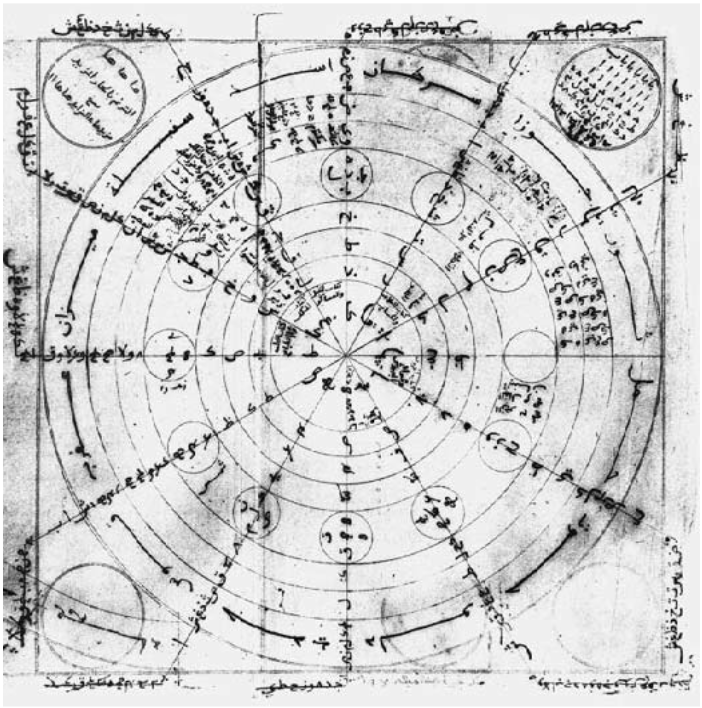
\includegraphics[width=0.49\textwidth]{ch2/images/zairjah_front.png}
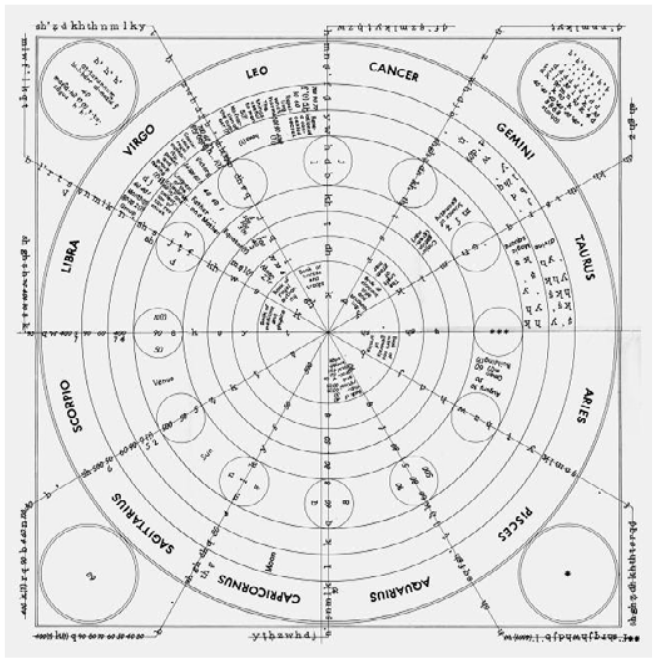
\includegraphics[width=0.49\textwidth]{ch2/images/zairjah_front_translation.png}\\
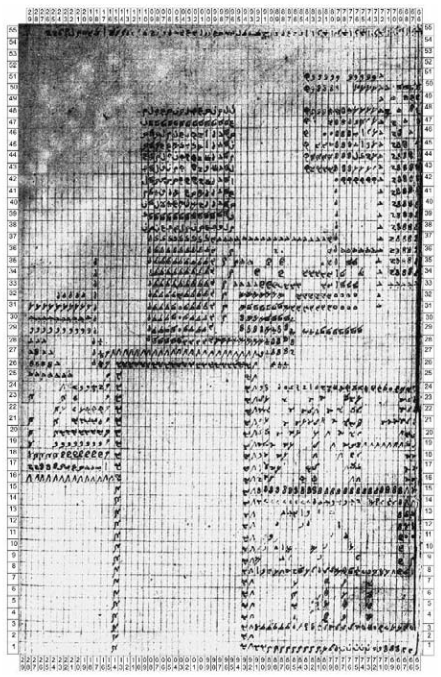
\includegraphics[width=0.6\textwidth,angle=90]{ch2/images/zairjah_back.png}
  
\caption{A z\={a}'irjah from a 15\textsuperscript{th} century Turkish
manuscript of the \textit{Muqaddimah} (top left), its English translation from
\cite{rosenthal1958muqaddimah} (top right), and its lookup table (bottom).
Images taken from \cite{link2010variantology}.}
\label{fig:zairjah}

\end{figure}

 
The z\={a}'irjah itself consists of a series of concentric circles divided
into 12 sections by six chords. The various segments of the diagram are
annotated with letters and numerals. Additionally, the z\={a}'irjah is
accompanied by a lookup table mapping letters to numbers. See
\autoref{fig:zairjah} for an example. According to painstaking reconstructions
done by \cite{link2010variantology}, a ``key poem'' was used to pose a
question to the z\={a}'irjah and serve as a mnemonic device/mapping of letters
to entries in the lookup table.  A combination of rules and astronomical
observations (antiquity's equivalent of a random seed) were then applied to
the key poem to read off series of characters from the z\={a}'irjah. The
operator would then interpret those letters into an answer.  ``The fact that
only consonants are written down in Semitic languages permits the meaningful
interpretation of many random permutations of symbols,''
\citep{link2010variantology} suggesting that cherry-picking outputs and
over-ascribing intelligence, knowledge, and even wisdom, to a language
generation algorithm are as old as the practice of NLG itself.
  
In a secondary account from a manuscript found at the library of Rabat in
Morroco, it is written that a skeptical ibn Khald\={u}n asked of the device
how old it was, ``[Is the] z\={a}'irjah [a] recent or [an] ancient science?''
Allegedly he received the answer, ``The  Holy  Spirit  will  depart,  its
secret having been brought forth / To Idr\={\i}s, and through it, he ascended
the highest summit,'' connecting the practice to the sage Idr\={\i}s who is
one of the eldest ancestors in the Quranic tradition
\citep{rosenthal1958muqaddimah,link2010variantology}.
  
The teachings of Arabic mystics, including the practice of z\={a}'irjah, as
well as the Kabbalistic tradition embodied in the \textit{Sefer Yetzirah} are
known to have strongly influenced the Majorcan Christian mystic, Ramon Llull
(1232-1315) \citep{kahn1980,link2010variantology,sepllull}.  Llull, who is
regarded as an early philosopher of combinatorics, logic, and computation
\citep{bonner2007art,knuth2013art,sepllull}, developed a computational system
based on moveable concentric circles made of paper and connected by string.
The workings of these \textit{volvelle}\footnote{The name \textit{volvelle}
comes from the Latin, literally ``to turn.''} are described in his master
work, \textit{Ars Magna} (1305). According to his system, concepts were
assigned letters which were manipulated to generate new statements involving
the concepts, and  he claimed could be used to determine the truth of any
proposition \citep{Crupi2019VolvellesOK}. Llull's work is also thought to have
influenced the polyalphabetic substitution cipher developed by Leon Battista
Alberti (1404 -- 1472) (see \autoref{fig:llull_volvelle}), the same core
cryptographic technology used in the Enigma machine  \citep{kahn1980}.

\begin{figure}[t]
    \centering

    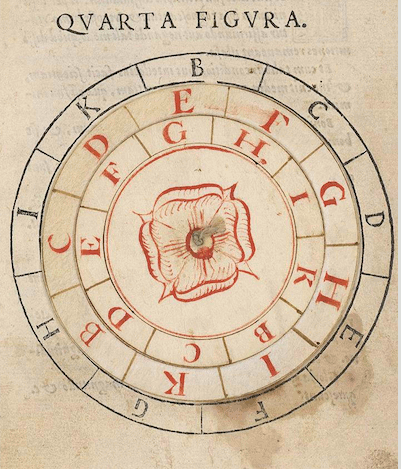
\includegraphics[width=0.45\textwidth]{ch2/images/llull_volvelle.png}\hfill
    
\includegraphics[width=0.45\textwidth]{ch2/images/alberti_cipher_disk.jpg}

\caption{(Left) A volvelle from  Llull's \textit{Ars Magnus} and (right)
Alberti's cipher disk.}
\label{fig:llull_volvelle}
\end{figure}


\begin{figure}[p]
    \centering
    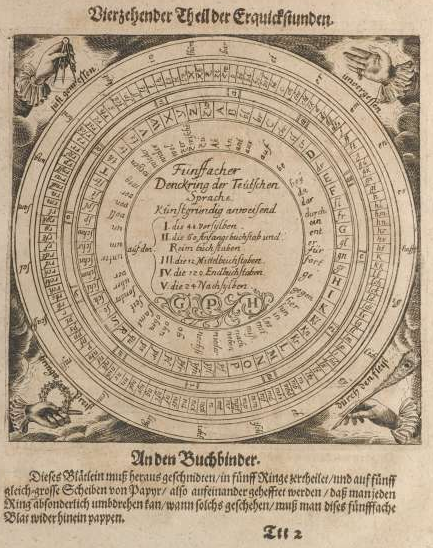
\includegraphics[width=0.98\textwidth]{ch2/images/baroque_volvelle.png}
  
\caption{An illustration of the German word generator volvelle, \textit{F{\"u}nffacher
Denckring der Teutschen Sprache} (1651) by Georg Philipp Harsd{\"o}rffer.}
\label{fig:baroque_volvelle}

\end{figure}
 
 
Llull's use of the volvelle as generative device was influential throughout
medieval Europe, where volvelle were used in both art and science. Arguably
they reached their zenith in the baroque works of Georg Philipp
Harsd{\"o}rffer (1607 -- 1658). His master work volvelle,
\textit{F{\"u}nffacher Denckring der Teutschen Sprache} (1651), consisted of
five paper discs (depicted in \autoref{fig:baroque_volvelle}), and was
designed to model German word formation. It was also advertised as an aid in
the production of poems and other literary  forms \citep{schafer2006literary}.
  
While computational devices before modern computing were limited in complexity
by their construction materials, chiefly paper, the dream of speaking automata
was also alive in myth.  See for example \autoref{fig:brazen_head}, in which a
17\textsuperscript{th} century woodcut print depicts a talking head capable of
answering any question. This ``brazen head'' was allegedly built by the monk
Roger Bacon, who in addition to being an early philosopher of science and
linguist, might also be considered the first NLP engineer if folklore is true
\citep{hyman2016automaton,sep-roger-bacon}.

\begin{figure}
    \centering
    \noindent
    {%
        \setlength{\fboxsep}{0pt}%
        \setlength{\fboxrule}{1pt}%
        \fbox{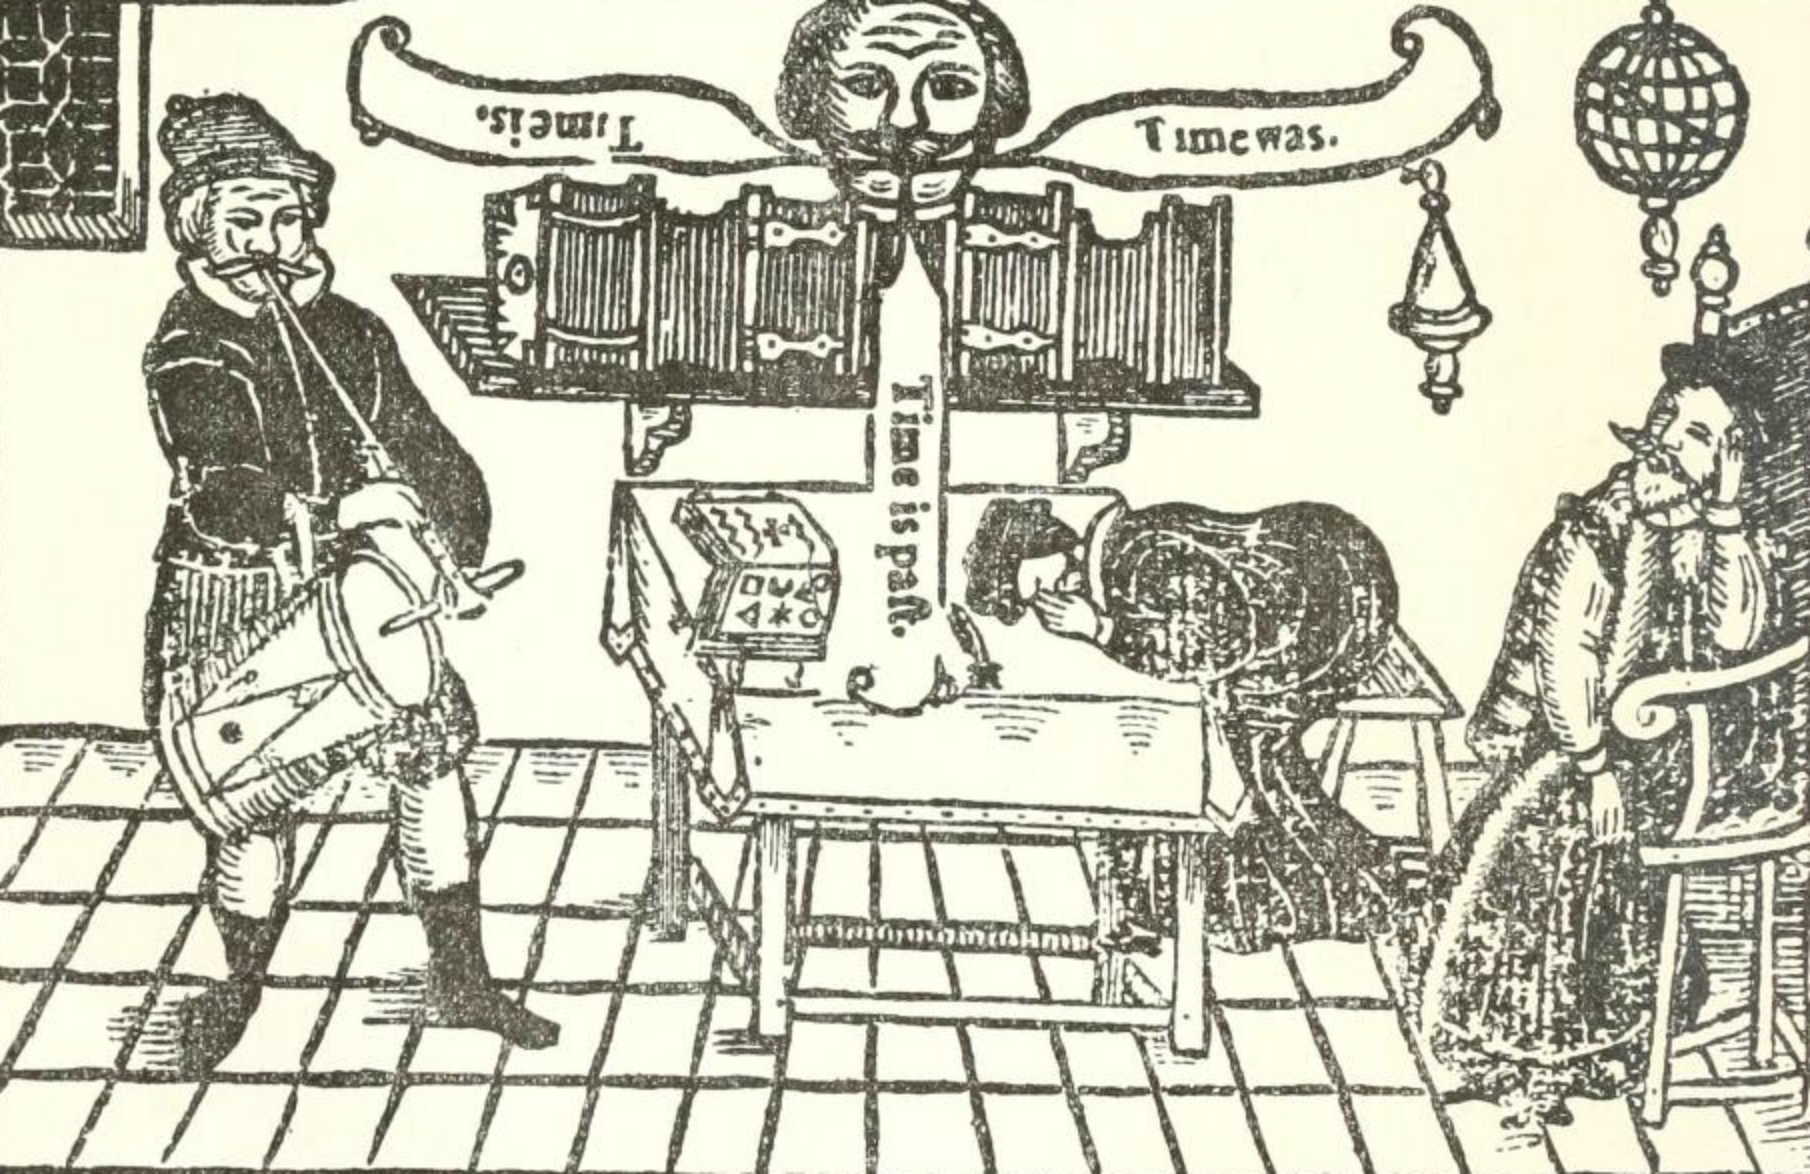
\includegraphics[width=0.7\textwidth]{ch2/images/brazen_head.png}}
    }

\caption{A 1630 woodcut depicting Roger Bacon's talking bronze head, a
mischievious talking autamata allegedly capable of answering any question.
Image taken from \cite{hyman2016automaton}.}
\label{fig:brazen_head}

\end{figure}
 
 

\section{Natural Language Generation from 1980--2000}
  
Returning to the present day, computer aided production of human language
closely follows the beginning of modern computing, starting with work on
machine translation (MT) systems developed in the 1950s and '60s
\citep{ornstein1955mechanical,national1966language,hutchins2003machine}. Early
work on producing extract summaries of research articles also dates back to
this period \citep{luhn1958automatic} as well as  also notable experiments in
generating text purely from syntactic structures \citep{yngve1961random}.
  
However, NLG did not begin to coalesce as a distinct subfield until the 1980s
which saw the first workshops devoted specifically to NLG  and a convergence
on the formalisms and problems central to language generation
\citep{reiter1997building,mcdonald2010natural}.  NLG researchers of this
period were focused on at least four main research programs: (i)
linguistically motivated grammars for generation, (ii) frameworks for
representing knowledge and concepts, (iii) models of the human receiver of the
generated text, and (iv) models of discourse and control for planning the
realization of utterances \citep{mann1981text,mckeown1986}. 
    
A variety of grammatical formalism were proposed during this period to be the
syntactic backbone of language generation algorithms, including Functional
Grammar \citep{halliday2013halliday}, Transformational Grammar
\citep{chomsky1965aspects}, Generalized Phrase Structure Grammar
\citep{gazdar1985generalized}, and others. Many frameworks for generation
proliferated at this time (often incorporating one of those grammar
formalisms), including Knowledge and Modalities Planner (KAMP)
\citep{appelt1982planning}, Penman \citep{hovy1993natural}, MUMBLE
\citep{McDonald1981MUMBLEAF}, TEXT \citep{mckeown1982text} and others
\citep{mann1981text}.  While there appears to be a great diversity of
approaches, over time the community began converging on a fairly similar
pipeline of modules when it came it implementation \citep{reiter1994has}. 
  
Indeed, most NLG systems from this period could be understood as a pipeline of
modules for text planning, sentence planning, and linguistic realization
\citep{reiter1997building}.  In the text planning stage, the concepts to be
conveyed are selected, possibly discarding less essential information, and
arranged into a discourse plan or ordering. In the sentence planning stage,
the concepts from the previous stage are grouped into individual sentences,
and lexicalizing concepts and referring expression generation is performed.
Finally, in linguistic realization, the intermediate representation from the
sentence planning stage is converted into a natural language utterance, often
by linearizing and inflecting some syntactic/morphological representation.
  
Since these systems primarily generated language by starting from
non-linguistic and/or semantic representations of concepts, they are often
referred to as \textit{concept-to-text} generation or, as more commonly known
today, \textit{data-to-text} generation \citep{gatt2018survey}. These systems
were applied to a variety of data-to-text problems including weather forecast
generation \citep{goldberg1994using}, statistical report  generation (i.e.
generating a report from numerical or statistical data in a spreadsheet)
\citep{iordanskaja-etal-1992-generation}, or as a writing aid to improve the
productivity of human authors \citep{springer1991,mckeown1994,paris1995}.
Data-to-text generation came to prominence alongside expert systems
\citep{todd1992introduction}, including as a means to explain them
\citep{swartout1983xplain}.  As such, these NLG systems suffer from some of
the same drawbacks as expert systems, often requiring extensive domain
knowledge and manual rule or grammar engineering which became  difficult to
maintain or amend over time.
  
In the late 1980s and into the 1990s, as larger text corpora became available
and statistical and/or machine learning techniques spread through the
community, text-to-text generation (i.e. methods of directly mapping
unstructured text inputs to text outputs) increased in popularity.
Text-to-text generation is less defined by a specific generation task, method
or unifying theory, but on the use of large collections of example
input/output text pairs. 
  
Statistical machine translation (SMT) emerges from this period as the dominant
success story for machine learning applied to text-to-text generation
problems.  The availability of digitized bilingual data made it possible to
create parallel sentence translation corpora and apply statistical word
alignment and translation techniques \citep{gale1993}.  The canonical IBM
translation models were developed in this period \citep{brown1988,brown1993}.
Statistical methods marked a stark improvement over attempts at interlingua or
semantics based translation systems which often required significant manual
effort in pre or post editing \citep{hutchins1994}. There were even some
limited experiments using learned classifiers to predict sentence salience for
summarization \citep{kupiec1995trainable}.

\section{The Emergence of Data Driven Extractive Summarization (2000--2014)}

While the MT community could take advantage of large (for the time) parallel
corpora,  it was not until the 2000s that there were readily available
collections of documents and their summaries for which to perform the kind of
supervised machine learning that was being successfully applied to MT.
Beginning in 2001, the Document Understanding Conferences (DUC) began steadily
producing collections of documents with reference summaries, bringing together
NLP researchers particularly around multi-document summarization
\citep{jones1999,harman2001,nenkova2005b}.
  
Many significant summarization systems from this time still relied on
unsupervised methods to create extract summaries, usually exploiting document
collection statistics to determine the salience of input text units.  The
representation of text units as TF-IDF weighted bags-of-words
\citep{jones1972} is prevalent in this era. For example, \cite{radev2000}
identify salience sentences in a document cluster by their similarity to the
average TF-IDF vector of the document cluster. In \cite{erkan2004}, sentences
are treated as vertices in a fully connected graph, with edge weights
determined by the cosine similarity between each sentence's TF-IDF weighted
bag-of-words representation. The PageRank algorithm \citep{page1999} is then
used to determine the graph centrality of each sentence; the sentences most
central in the graph are considered the most salient and extracted for the
summary. 

Other methods used alternative formulations to exploit frequency for
summarization, most notably \cite{lin2000} who identified topic signatures
using a likelihood ratio test \citep{dunning1993} to identify terms that
occurred unusually frequently in a document given a large generic background
corpus. After removing stopwords, word frequency on its own has also been
shown to be an effective signal for identifying salient sentences
\citep{nenkova2005}.

Following on the initial research by \cite{kupiec1995trainable}, other work
using supervised learning for summarization begins to emerge from this time
\citep{conroy2001using,osborne2002using,hirao2002extracting,sipos2012large}.
Here, summarization is framed as a sentence classification task (i.e., which
sentences from the input document should be included in a summary). 

Most of the text-to-text summarization approaches from the 2000s are primarily
extractive systems.  While significantly constrained in their expressive
quality (i.e. only sentences found in the input can be used to construct the
output) especially compared to earlier data-to-text methods, designing
data-driven features for unsupervised and supervised statistical machine
learning proved to be much more scalable and an easier path to improved
summarization performance \citep{nenkova2011}. 
 
There are some notable works that attempted to perform limited abstractive
summarization. \cite{barzilay2005}  developed an unsupervised method of
sentence fusion (i.e., combining sentences with the same or overlapping
content using their syntactic parses as backbone structure), that has been
extended and  refined by others \citep{marsi2005,filippova2008}. Heuristically
driven phrase deletions were also explored to reduce less salient information
in extractive summarization \citep{jing2000,zajic2007}.  In the supervised
case, there were several works that attempted to learn to  delete
non-essential phrase constituents.  This was formulated as either a pipeline
of learned compression and extraction models \citep{wang2013} or as a joint
model of extraction and compression \citep{martins2009,bergkirkpatrick2011}.
While sentence fusion was capable of some abstractive rewriting, the other
approaches mentioned here predominantly focused on compression, i.e. word or
phrase deletion, to generate novel summary text, which is only one of the many
ways that human abstractors perform the summarization task \citep{jing2000b}.

Streaming or temporal summarization was first explored in the context of topic
detection and tracking \citep{khandelwal2001,allan2001} and more recently at
the Text Retrieval Conference (TREC) \citep{aslam2013}. Approaches to this
problem often perform filtering by estimated salience before relying on
multi-document summarization techniques to select text units to construct
rolling update summaries \citep{guo2013,mccreadie2014}. These pipelines while
effective, do not attempt to jointly optimize the salience and selection.

\section{Neural Natural Language Generation Models (2014--Present)}
  
While feed-forward neural networks had been used previously as part of
phrased-based SMT systems \citep{schwenk2006}, there was an increased interest
in the early-mid 2010s around using recurrent neural network (RNN) language
models \citep{mikolov2010} as a rescoring method for an SMT decoder
\citep{auli2013,cho2014learning}.  RNNs could exploit (in theory) unbounded
source and target prefix information that was difficult to capture in ngram or
feed-forward models. \citet{cho2014learning} is particularly notable because
they propose separate encoder/decoder RNNs, and while intended for rescoring
and not generation directly, this general architecture constitutes the
``sequence-to-sequence'' backbone of most neural MT (NMT) and neural NLG
models.
  
Shortly thereafter, \citet{sutskever2014} proposed the now ubiquitous
sequence-to-sequence model to perform translation directly.
\citet{bahdanau2015}  also proposed a sequence-to-sequence model with an
attention mechanism, which both made optimization easier (error feedback, i.e.,
gradients, could now be routed directly from any decoder word prediction step
to any arbitrarily  distant timesteps in the encoder) and allowed for
visualization of the NMT decoder's alignment with the encoder.  NMT models,
while conceptually simpler than phrase-based SMT, were starting to achieve
state-of-the-art results \citep{bojar2016} and wide-spread industry adoption
\citep{wu2016google,gehring2017}.  It did not take long for researchers to
adapt the sequence-to-sequence model to other language generation problems,
e.g. generating captions from images \citep{vinyals2015a}, sports summaries for
box scores \cite{lebret2016,wiseman2017}, or from semantic representations
\citep{wen2015,dusek2016}. 
  
The introduction of the CNN-DailyMail corpus by \cite{hermann2015} allowed for
the application of large-scale training of deep learning models for
summarization. In sentence extractive summarization, researchers proposed a
variety of hierarchical models with distinct sentence and document level
encoder networks that enabled sequential prediction of which sentences or words
should be included in the summary
\citep{cheng2016neural,nallapati2017summarunner}.

Perhaps more exciting was the surge in abstractive summary generation.
\cite{rush2015} developed an attention-based deep learning  model capable of
generating headlines from the lead sentence of an article. Subsequently,
\citet{nallapati2016} showed that a sequence-to-sequence model could encode a
whole news article and then generate an abstractive summary word by word.
Additionally, the line between extractive and abstractive summarization was
blurred by the addition of learned copy-mechanisms which could selectively
transfer named entities and other out-of-vocabulary terms into the output
summary, further improving summary quality \citep{see2017}.  

Historically, the field of NLG has relied heavily on grammars and templates to
generate text. The fact that neural models could yield reasonably fluent and
acceptable summaries given so little pre-specified structure or features is
truly impressive.  Interestingly, term frequency, was not explicitly
represented in either the neural extractive or abstractive summarization
models, begging the question as to how they were learning to identify salient
content.

Model architecture continued to evolve and in \citeyear{vaswani2017},
\citeauthor{vaswani2017} proposed a recurrence-free neural sequence model,
built around so-called \textit{transformer} layers, which rely on multiple
parallel self- and context-attention mechanisms.  This model was designed with
optimization speed in mind, and was subsequently used in large scale language
model pretraining on web-scale text, spawning the BERT-family of models
\citep{devlin2019}. Large language model pre-training with task-specific
fine-tuning became a dominant paradigm in NLP with BERT and its descendants
setting records on many downstream text prediction tasks \citep{ruder2019}.

The transformer layer was also used in the generative pre-training (GPT)-family
of models \citep{radford2018improving}, which was  also trained on web-scale
data, but with an auto-regressive language modeling objective.  The second
generation of these models, GPT-2 \citep{radford2019}, received notoriety both
amongst NLP researchers but also the wider public, as its release was initially
delayed given ``ethical concerns'' about releasing such a powerful language
generation model \citep{vincent2019,seabrook2019}.  GPT-2 exhibited impressive
completions of prompt texts, and could be used to generate natural looking
paragraphs on arbitrary topics, with longer spans of fluent text than
previously thought possible. 
  
GPT-2 could also be fine-tuned to perform task specific conditional generation
\citep{ziegler2019,golovanov2019}, however, its architecture was that of a
neural language model without distinct encoder/decoder networks; conditional
generation was achieved by encoding problem instances as prompts to be
continued.  Proper sequence-to-sequence variants of the large,
transformer-based language model were subsequently developed using various
sequence-level denoising autoencoder objectives \citep{zhang2019,raffel2020,
lewis2020}.  The intention of such models was that they could be fine-tuned for
more task-specific sequence-to-sequence problems like summarization,
translation, or even arbitrary data-to-text tasks like dialogue generation.

While these models were producing text at a level of quality that had not
previously been realized with traditional NLG approaches, a closer examination
of model outputs revealed glaring flaws in the semantic correctness of the
generated text \citep{kryscinski2019,kryscinski2020,maynez2020}.
\cite{dusek2020} found that the quality of neural NLG models can vary
significantly, with relatively similar architectures yielding both poor and
competitive performance with respect to the semantic correctness of model
outputs. In practice most competitive neural NLG models use a variety of beam
reranking techniques to improve output faithfulness to the inputs
\citep{dusek2016,juraska2018,wen2015}, as well as copy and coverage mechanisms
to improve the recall \citep{see2017,elder2018}.

NLG researchers have also begun to explore the degree to which neural models
can be constrained to follow discourse plans or other structured objects.
\citet{nayak2017} and \citet{reed2018} explore several ways of incorporating
shallow sentence planning into dialogue generation via the  grouping of input
sequences into distinct subsequences or by inserting discourse variable tokens
into the encoder input sequences to indicate contrasts, comparisons, or other
groupings.  \citet{balakrishnan2019} experiment both with tree structured input
meaning representations  and encoders and compare them to linearized trees with
standard sequence-to-sequence models.  While these papers find that neural NLG
models can consistently follow these discourse ordering constraints, they do
not  systematically explore how other linearization strategies compare in terms
of faithfulness, and they do not evaluate the degree to which a
sequence-to-sequence model can follow realization orders not drawn from the
training distribution.

\citet{castroferreira2017} compare a neural NLG model using various
linearizations of abstract meaning representation (AMR) graphs, including a
model-based alignment very similar to the alignment-training linearization
presented in this work. However, they evaluate only on automatic quality
measures and do not explicitly measure the semantic correctness of the
generated text or the degree to which the model realizes the text in the order
implied by the linearized input.

Works like \citet{moryossef2019a,moryossef2019b} and \citet{castroferreira2019}
show that treating various planning tasks as separate components in a pipeline,
where the components themselves are implemented with neural models, improves
the overall quality and semantic correctness of generated utterances relative
to a completely end-to-end neural NLG model. However, they do not test the
``systematicity'' of the neural generation components, i.e. the ability to
perform correctly when given an arbitrary or random input from the preceding
component, as we do here with the random permutation stress test.

Many papers mention input linearization order anecdotally but do not quantify
its impact. For example, \citet{juraska2018} experiment with random
linearization orderings during development, but do not use them in the final
model or report results using them, and \citet{gehrmann2018} report that using
a consistent linearization strategy worked best for their models but do not
specify the exact order.  \citet{juraska2018} also used sentence level data
augmentation, i.e. splitting a multi-sentence example in multiple single
sentence examples, similar in spirit to our proposed phrase based method, but
they do not evaluate its effect independently.  \citet{wiseman2018} uses an
order invariant encoder to produce a latent plan which guides the decoder.
Ignoring the encoder and specifying a latent plan would allow for some control
over realization order but the degree to which arbitrary realization orders can
be achieved is under explored. Additionally, it is not guaranteed that latent
plan states uniquely correspond to different meaning representation components.


%%%%%%%%%%%%%%%%%%%%%%%%%%%%%%%%%%%%%%%%%%%%%%%%%%%%%%%%%%%%%%%%%%%%%%%%%%%%%%%
%                                                                             %
% Chapter 3: Salience Estimation with Deep Learning Content Selection Models  %
%                                                                             %
%%%%%%%%%%%%%%%%%%%%%%%%%%%%%%%%%%%%%%%%%%%%%%%%%%%%%%%%%%%%%%%%%%%%%%%%%%%%%%%

\chapter{Salience Estimation with Deep Learning Content Selection Models}
\label{ch:dlsum}

\startglyph Salience estimation, that is, the prediction of the importance or
relevance of a unit of text, is a critical step for any text summarization
algorithm \citep{nenkova2011}. Since the size of the desired output summary is
constrained to be much smaller than the original document or documents being
summarized, it is necessary to prioritize some information over others when
deciding the content of  the summary. Estimating the salience of various units
of text (i.e., words, phrases, sentences, etc.) enables summarization
algorithms to perform this prioritization.

There is no universally agreed upon definition of salience, so its estimation
starts on rather shaky epistemological ground. What is most salient will vary
significantly from reader to reader, and depend largely on their particular
information need and/or prior knowledge \citep{jones1999}.  In this chapter, we
focus on a supervised learning scenario, where the training corpus consists of
a single document paired with a human reference abstract summary prepared by a
domain expert. In this setting,  we can rely on a data-driven definition of
salience; information that the domain expert has put in the summary is most
salient.  By matching units of text in the input document to corresponding text
units in the summary, we label the document text units with a binary judgement
of salience (see \autoref{sec:labelgen} for details). 

If we set the basic unit of text to be a single sentence and we obtain binary
salience judgements in the manner described above, we can model sentence
extractive single document summarization as a sequence labeling task
\citep{conroy2001}. In this formulation, a document is a sequence of sentences,
and the task objective is to predict the salience judgment for each sentence.
In the simplest of settings, the actual extract summary can be formed by
concatenating the sentences labeled as salient.

We refer to the probability of a sentence being labeled as salient as the
salience estimate.  Historically, most machine learning based methods for
salience estimation have use \featurebased~representations of text units to
make salience estimates. Typically, these features make use of word level
frequency data \citep{nenkova2005}, information theoretic notions of surprise
or topicality \citep{lin2000,daume2006,louis2013,louis2014}, as well as
position based features (e.g., is the unit of text in the beginning, middle, or
end of the document?) \citep{kupiec1995trainable,radev2000,conroy2001}, which
are often correlated with human judgements of salience \citep{nenkova2005b}.

The field of summarization has undergone a revolution driven by the recent
popularization of deep learning based models in NLP.  Deep learning models have
demonstrated empirical successes, achieving state-of-the-art performance in
both extractive \citep{cheng2016neural,nallapati2017summarunner} and
abstractive summarization settings \citep{nallapati2016,see2017,zhang2019}.
Deep learning models also naturally allow for learning hierarchical
representations of word, sentence, and document level contexts when performing
end-to-end training on the summarization task.  However, exactly what kind of
information is captured in these representations and how that information
affects downstream salience estimation has not been experimentally verified. 

In this chapter, we systematically compare several supervised deep learning
models of sentence extractive single document summarization.  As in prior work,
we model a document hierarchically: a document is a sequence of sentences and a
sentence is a sequence of words.  Each summarization model consists of three
layers or modules: 
\begin{enumerate}
\item The word embedding layer, which maps sequences of words to sequences of
    fixed dimensional embeddings. 
\item The \sentenceencoder~layer, which maps sequences of word embeddings to a
    sentence embedding. 
\item The \sentenceextractor~layer, which maps sequences of sentence
    embeddings to a sequence of salience judgements.
\end{enumerate}

We systematically compare three different architectures for the
\sentenceencoder~and four different \sentenceextractor~architectures.
Additionally, we also measure the effect of using fixed pretrained embeddings
versus fine-tuning embeddings while training the rest the of model.  Various
configurations of encoder and extractor modules correspond to both prior work
by \cite{cheng2016neural} or \cite{nallapati2017summarunner} as well as novel
summarization models. While prior works have primarily used
\autoregressive~\sentenceextractor~architectures, we propose two
\nonautoregressive~\sentenceextractor s.  We evaluate these models across a
range of domains including large and small news domains, as well as personal
stories, meetings, and medical research articles. 

Additionally, we systematically ablate the inputs to models during training to
better understand what surface level features are being used to make
predictions. Words are tagged with a \partofspeech~tagger and different word
classes are replaced with special \emph{unknown} tokens.  We can then compare
performance of the summarization model with and without access to specific
classes of word features (e.g., nouns or verbs). To ablate the implicit effects
of sentence position, we compare models trained on the original document to the
same model trained on documents with shuffled sentence order.  By removing
content and position features, we can see their relative impact in the decrease
in \rouge~scores on the test set. Moreover, these ablations give us a more
intuitive understanding of how models will behave in novel environments. For
example, if we know position is an important feature for a model, using it on
data that is not position biased will likely result in poor performance.

Our main results  reveal:
\begin{enumerate}
\item Sentence position bias dominates the learning signal for news
    summarization, though not for other domains. Summary quality for news is
    only slightly degraded when content words are omitted from sentence
    embeddings.
\item Word embedding averaging is as good or better than either recurrent
    or convolutional encoders
    for sentence embeddings across all domains.
\item  Pre-trained word embeddings are as good, or better than, learned
    embeddings in five of six datasets.
\item Non auto-regressive sentence extraction performs as good or better than
    auto-regressive extraction in all domains.
\end{enumerate}

Taken together, these and other results in the paper suggest that we are
over-estimating the ability of deep learning models to learn robust and
meaningful content features for summarization. In one sense, this might lessen
the burden of applying neural network models of content to other domains; one
really just needs in-domain word embeddings. However, if we want to learn
something other than where the start of the article is, we will need to design
other means of sentence representation, and possibly external knowledge
representations, better suited to the summarization task.

\section{Problem Definition}

We now formally define the sentence extractive, single document summarization
task as a sequence tagging problem, following \cite{conroy2001}.  Let a
document $\doc\in \docSpace$ be a sequence of $\docSize$ sentences, 
\[ 
    \doc = \left[ \sent_1, \sent_2, \ldots, \sent_\docSize\right].
\] 
Sentences are themselves sequences of words,
\[
    \sent_i=\left[
        \word_{i,1}, \word_{i,2}, \ldots, \word_{i,{\sentSize_i}}\right],
\]
where $\sentSize_i\in\naturals$ is the length of sentence $\sent_i$ in words.
The words themselves are drawn from a finite vocabulary $\wordVocab$.

The binary \salience~of a sentence $\sent_i$ is $\bsal_i \in\{0,1\}$.
$\bsal_i=1$ indicates that sentence $\sent_i$ is \salient~and should be
included in the extract summary while $\bsal_i=0$ is assigned to
non-\salient~sentences that should be excluded from the summary.  We indicate
the vector of salience judgements for the $\docSize$ sentences in $\doc$ as
$\bsals = \left[\bsal_1,\ldots,\bsal_\docSize\right]\in  \labelSpace$.  The
objective of this sequence tagging problem is to learn a function $f :
\docSpace \rightarrow \labelSpace$ which maps a document $\doc$ to a sequence
of \salience~labels $\bsals$. In this work, we learn a probabilistic mapping
$\model(\bsals|\doc;\params)$ where $\model$ is a neural network with
parameters $\theta$ and $\model(\cdot|\doc;\params) : \labelSpace \rightarrow
(0,1)$. 

Prediction is achieved by finding $\predbsals = \operatorname{arg\;max}_{\bsals
\in \labelSpace} \model(\bsals|\doc;\params)$, either by approximation or when
the structure of $\model$ allows, exactly.  Additionally, a typical constraint
on summarization is that the extract summary not exceed a word budget
$\wordbudget \in \naturals$, that is, $\sum_{i=1}^\docSize \hat{\bsal}_i \cdot
\sentSize_i \le \wordbudget$.  Since it is not trivial to incorporate this
constraint into the sequence labeling formulation, we instead rely on a greedy
heuristic to enforce the budget constraint in practice. More details on test
time inference can be found in \autoref{sec:inference}.

\section{Models}

We implement our salience estimation model $\nnmodel(\nnsals|\nndoc;\params)$
hierarchically following the analogous structure of the documents we are
modeling.  Every model $\nnmodel$ proposed in this chapter consists of three
modules or layers: \textit{(i)} the word embedding layer, \textit{(ii)} the
sentence encoder layer, and \textit{(iii)} the sentence extractor layer.  The
word embedding layer maps the words in a sentence to a sequence of word
embeddings. The sentence encoder layer similarly maps sequences of word
embeddings to a sentence embedding. Finally, the sentence extractor maps
sequences of sentence embeddings to sequence of salience labels.

Choosing an architecture for each of the modules defines the model. We define
several architectures for the sentence encoder and extractor layers and show
how particular settings of each correspond to prior summarization models
proposed by \citet{cheng2016neural} and \citet{nallapati2017summarunner}.
Additionally, we propose two novel sentence extractor layers, and in
experiments consider all combinations of sentence encoder/extractor pairings.
In the next subsections, we describe each layer in more detail, and conclude
this section showing how certain configurations of each layer maps to
previously proposed or novel salience estimation models and how the models
generate an extract summary at test time (which we refer to as inference).

\subsection{Word Embedding Layer}

The word embedding layer, $\embLayer(\cdot\,;\embParams) : \wordVocab^*
\rightarrow \reals^{* \times \embDim},$ maps a sequence of words 
\[
    \sent_i = \left[\word_{i,1},\ldots, \word_{i,\sentSize_i}\right]
\] 
to a sequence of word embeddings 
\[
\nnwordEmbs_i = \left[ \wordEmb_{i,1}, \ldots, \wordEmb_{i,\sentSize_i} \right]
    \in \reals^{\sentSize_i \times \embDim}
\]
where the sole parameter $\embParams \in \mathbb{R}^{|\wordVocab| \times
\embDim}$ is a $\embDim$-dimensional embedding matrix and $\wordEmb_{i,j} =
\embParams_{\word_{i,j}}$ is the word embedding for word $\word_{i,j}$.
$\embParams$ is initialized prior to training the full model with embeddings
obtained using the unsupervised Global Vector (GloVe) embedding method on a
large collection of text \citep{pennington2014glove}.  Additionally,
$\embParams$ can be held fixed during training or updated with other model
parameters. We use $\embDim = 200$-dimensional embeddings in our models.

\begin{figure}
\begin{subfigure}{\textwidth}
  \centering
  %\includegraphics[width=.8\linewidth]{images/ch2/avgsentencoder.pdf}
  \includegraphics{images/ch2/avgsentencoder.pdf}
  \caption{Averaging Sentence Encoder}
  \label{fig:sfig1}
\end{subfigure}

\begin{subfigure}{\textwidth}
  \centering
  %\includegraphics[width=.8\linewidth]{images/ch2/cnnsentencoder.pdf}
  \includegraphics{images/ch2/rnnsentencoder.pdf}
  \caption{\RecurrentNeuralNetwork~Sentence Encoder}
  \label{fig:sfig2}
\end{subfigure}

\begin{subfigure}{\textwidth}
  \centering
  %\includegraphics[width=.8\linewidth]{images/ch2/cnnsentencoder.pdf}
  \includegraphics{images/ch2/cnnsentencoder.pdf}
  \caption{\convolutionalneuralnetwork~Sentence Encoder}
  \label{fig:sfig2}
\end{subfigure}
    \caption{Schematics for the averageing, \recurrentneuralnetwork,
    and \convolutionalneuralnetwork~sentence encoders.}
\label{fig:sentenceEncoders}
\end{figure}




\subsection{Sentence Encoder Layer} \label{sec:senc}

The sentence encoder layer, \sentEncFuncDef, maps a sequence of word embeddings
\[
\nnwordEmbs_i = \left[\wordEmb_{i,1},\ldots, \wordEmb_{i,\sentSize_i}\right]
\] 
to a $\sentDim$-dimensional embedding representation of sentence $\sent_i$.
The set of associated parameters, $\sentEncParams$, depends on the exact
architecture for implementing the encoder. We experiment with three
architectures for mapping sequences of word embeddings to a fixed length
vector: averaging, recurrent neural networks, and convolutional neural
networks.

We describe each variant now, and also briefly discuss the trade-offs
associated with each architecture. The main distinction amongst the encoders is
to how they can exploit the context and structure of the words they are
encoding. With the averaging encoder, the resulting sentence embedding captures
all words equally, but is insensitive to phrase structure phenomenon like
negation. The convolutional encoder can capture local phrase structure but may
not be able to capture long range phrase structure. The recurrent encoder can
capture long range phrase structure and context but is computationally more
expensive than the recurrent encoder.  Schematics of each encoder architecture
can be found in \autoref{fig:sentenceEncoders}.

\subsubsection{Averaging Sentence Encoder} 

Under the averaging encoder, a sentence embedding $\sentEmb_i \in
\reals^{\sentDim}$ is simply the average of its word embeddings,
\begin{align} 
    \sentEmb_i & = \sentEnc(\nnwordEmbs_i;\sentEncParams) =  
        \frac{1}{\sentSize_i} \sum_{j=1}^{\sentSize_i} \wordEmb_{i,j}.
\end{align}
The sentence representation here is effectively a bag of word embeddings.
There are no parameters associated with this encoder (i.e.  $\sentEncParams =
\emptyset$). The size of the sentence embedding is simply $\sentDim = \embDim =
200$. Dropout with drop probability 0.25 is applied to each word embedding
$\wordEmb_{i,j}$ during training. 

\subsubsection{\RecurrentNeuralNetwork~Sentence Encoder} 

When using the \recurrentneuralnetwork~encoder we apply both forward and
backward \recurrentneuralnetwork s over the word embedding sequences produced
by the embedding layer. To obtain the actual sentence embedding, we concatenate
the final output step of the forward and backward networks.  For the actual
recurrence function, we use the \gatedrecurrentunit~(GRU)
\citep{cho2014learning}.  The GRU function, $\gruFuncDef{\embDim}{\hidDim}$, is
defined as
\begin{align}
\fgru(\wordEmb, \sentEmb; \varphi) & 
    = (1-\GRUupdategate) \odot \GRUcandgate + \GRUupdategate \odot \sentEmb \label{eqn:gru}\\
    \textit{(Reset gate)} & \nonumber \\
\GRUresetgate &= 
    \sigma\left(
      \GRUWeight^{(\wordEmbChar\GRUresetchar)} \wordEmb 
        + \GRUBias^{(\wordEmbChar\GRUresetchar)} +
      \GRUWeight^{(\sentEmbChar\GRUresetchar)} \sentEmb 
        + \GRUBias^{(\sentEmbChar\GRUresetchar)} 
    \right)\\
    \textit{(Update gate)} & \nonumber \\
\GRUupdategate &= 
    \sigma\left(
      \GRUWeight^{(\wordEmbChar\GRUupdatechar)} \wordEmb 
        + \GRUBias^{(\wordEmbChar\GRUupdatechar)} +
      \GRUWeight^{(\sentEmbChar\GRUupdatechar)} \sentEmb 
        + \GRUBias^{(\sentEmbChar\GRUupdatechar)} 
    \right)\\
    \textit{(Candidate state)} & \nonumber \\
\GRUcandgate &= \tanh\left(
    \GRUWeight^{(\wordEmbChar\GRUcandchar)} \wordEmb 
        + \GRUBias^{(\wordEmbChar\GRUcandchar)} + 
    \GRUresetgate \odot \left(
        \GRUWeight^{(\sentEmbChar\GRUcandchar)} \sentEmb 
            + \GRUBias^{(\sentEmbChar\GRUcandchar)} 
    \right) \right)
\end{align}
where $\GRUparams = \left\{   \GRUWeight^{(ab)}, \GRUBias^{(ab)} \Big\vert a
\in \{v,h\}, b \in \{r,u,o\} \right\}$ is the set of \gru~parameters with
$\GRUWeight^{(\wordEmbChar\cdot)} \in \reals^{\hidDim \times \embDim}$,
$\GRUWeight^{(\sentEmbChar\cdot)} \in \reals^{\hidDim \times \hidDim}$, and
$\GRUBias^{(\cdot)} \in \reals^{\hidDim }$, and $\sigma(x) =
\frac{1}{1+e^{-x}}$, $\tanh(x) = \frac{e^x-1}{e^x+1}$, and $\odot$ is the
Hadamard product.
 

Under the \recurrentneuralnetwork~encoder, a sentence embedding $\sentEmb_i$ is
then defined as
\begin{align} 
  \sentEmb_i = \sentEnc\Big(\nnwordEmbs_i; \sentEncParams\Big) & = \left[
                \begin{array}{l}\rSentEmb_{i,\sentSize_i}\\ \lSentEmb_{i,1}
    \end{array}
  \right] \\
  \textit{(Forward GRU)} \nonumber & \\
  \rSentEmb_{i,0} &= \zeroEmb, \\ 
  \rSentEmb_{i,j} &= 
      \fgru(\wordEmb_{i,j}, \rSentEmb_{i,j-1}; \rSentGRUParams) 
      & \forall j \in \{1,\ldots,\sentSize_i\} \\  
  \textit{(Backward GRU)} \nonumber & \\
  \lSentEmb_{i,\sentSize_i + 1} &= \zeroEmb, \\
  \lSentEmb_{i,j} &= 
      \fgru(\wordEmb_{i,j},\lSentEmb_{i,j+1}; \lSentGRUParams)
      & \forall j \in \{\sentSize_i, \ldots, 1\} 
\end{align}
where $[\cdots]$ is the vector concatenation operator and $\rSentGRUParams$ and
$\lSentGRUParams$ are distinct parameters for the forward and backward GRUs
respectively.  Collectively the set of parameters for the recurrent neural
network sentence encoder is $\sentEncParams = \left\{ \rSentGRUParams,
\lSentGRUParams \right\}$. We use $\hidDim=300$ dimensional hidden layers for
each \gru, making the size of the sentence embedding $\sentDim=2\hidDim=600$.
Dropout with drop probability $0.25$ is applied to \gru~outputs
$\rSentEmb_{i,j}$ and $\lSentEmb_{i,j}$ for $j \in \{1,\ldots,\sentSize_i\}$
during training.

\subsubsection{\ConvolutionalNeuralNetwork~Sentence Encoder} 
\label{sec:sentconvenc}

The \convolutionalneuralnetwork~sentence encoder uses a series of convolutional
feature maps to encode each sentence. This encoder is similar to the
convolutional architecture of \citet{kim2014convolutional} used for text
classification tasks. It performs a series of ``one-dimensional'' convolutions
over word embeddings. The \kernelwidth~$\ckernelWidth \in \naturals$ of a
feature map determines the number of contiguous words that a feature map is
sensitive to. For $\ckernelWidth=3$, for example, the feature map would
function as a trigram feature detector essentially.  We denote a single
convolutional feature map of kernel width $\ckernelWidth$ as
$\ckernel_\ckernelWidth : \reals^{*\times \embDim} \rightarrow \reals$ with
\begin{align}
    \ckernel_\ckernelWidth(\wordEmb_i;\upsilon,\beta)  & 
= \max_{j \in \{ 
    1 - \left\lfloor \frac{\ckernelWidth}{2} \right\rfloor, 
    \ldots, \sentSize_i +  
    \left\lfloor \frac{\ckernelWidth}{2} \right\rfloor - \ckernelWidth + 1 \}}
  \relu\left( \cBias + \cMatrix \cdot \left[ \begin{array}{c} \wordEmb_{i,j}\\ \wordEmb_{i,j+1} \\ \vdots \\ \wordEmb_{i,j+k-1} \end{array} \right] \right),
\end{align}
where $\relu(x) = \max(0, x)$ is the rectified linear unit \citep{nair2010},
$\left\lfloor\cdot\right\rfloor$ is the floor operator, and $\cMatrix \in
\reals^{\ckernelWidth \embDim}$ and $\cBias \in \reals$ are learned parameters.
Note that we use a ``zero-padded'' convolution \citep{dumoulin2016}. That is,
the $\max$ operator ranges over  $j \in \left\{1 - \left\lfloor
\frac{\ckernelWidth}{2} \right\rfloor, \ldots, \sentSize_i +  \left\lfloor
\frac{\ckernelWidth}{2} \right\rfloor - \ckernelWidth + 1 \right\}$ instead of
$\left\{1,\ldots,\sentSize_i - \ckernelWidth + 1\right\}$, and $\wordEmb_{i,j}
= \zeroEmb$ for $j < 1$ and $j > \sentSize_i$. Padded convolutions help
alleviate the problem of reduced receptive fields on the boundaries of the
sequence. See \autoref{fig:paddedconv} for a visual example.

\begin{figure}
\centering 
\fbox{\resizebox{\textwidth}{!}{
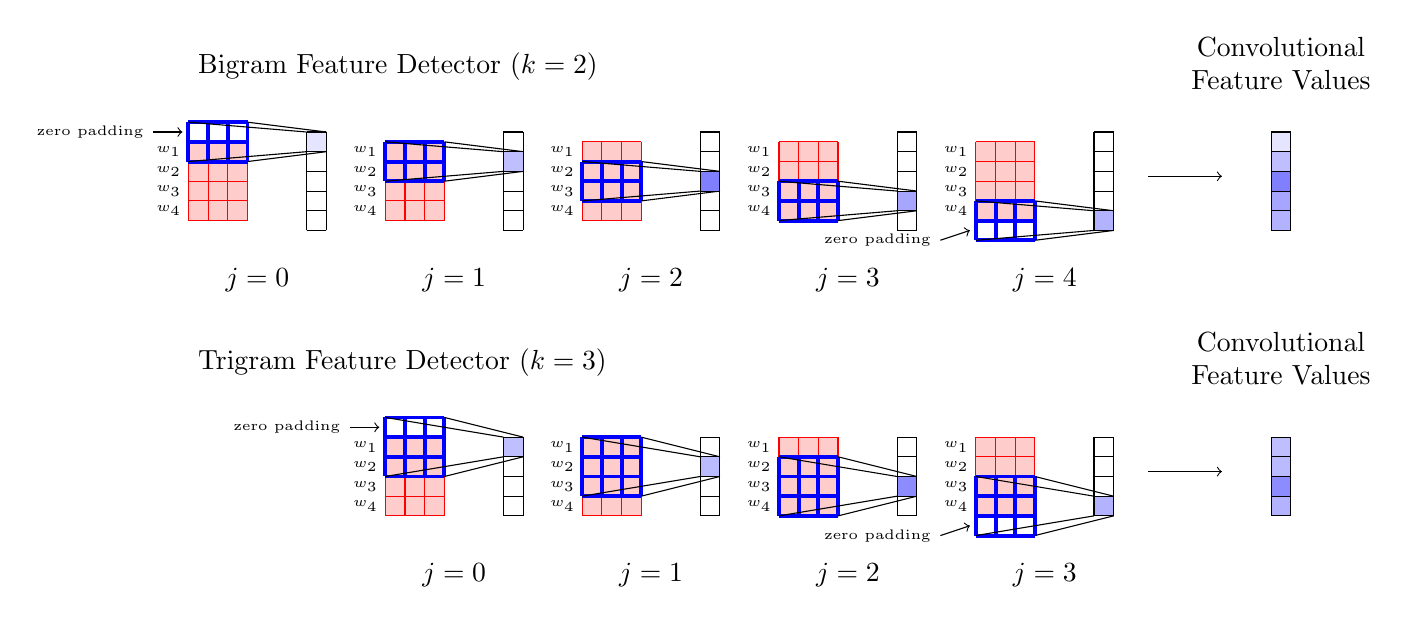
\begin{tikzpicture}[x=0.25cm, y=0.25cm,
    embs/.style={step=0.25cm,red},
    bigram/.style={step=0.25cm,blue,line width=0.5mm},
  convcon/.style={black,line width=0.5mm},
  hid/.style 2 args={
    rectangle split,
    draw=#2,
    rectangle split parts=#1,
    fill=#2!20,
    outer sep=1mm}]

\def\SEP{10}
\def\YSEP{15}

\foreach \a [count=\step from 1,
             evaluate=\step as \smo using int(\step - 1),
             evaluate=\step as \fnwx using \SEP*\step+3,
             evaluate=\step as \fnwy using 4-\step+2,
             evaluate=\step as \fsex using \SEP*\step,
             evaluate=\step as \fsey using 4-\step,
             evaluate=\step as \anwx using \SEP*\step+7,
             evaluate=\step as \anwy using 5-\step+1-0.5,
             evaluate=\step as \asex using \SEP*\step+6,
             evaluate=\step as \asey using 5-\step-0.5,
] in {10,25,50,35,30} {

    \foreach \i [count=\w from 1] in {1,...,4} {
        \node[font=\tiny] at (\SEP*\step-1,5-\i-0.5) {$w_\w$};
    }
    \fill[red!20!] (\SEP*\step,0) rectangle (\SEP*\step+3,4);
    \draw[embs] (\SEP*\step,0) grid (\SEP*\step+3,4);
    
    \draw[bigram] (\fsex,\fsey) grid (\fnwx,\fnwy);
    
    \draw (\fsex,\fnwy) -- (\asex,\anwy);
    \draw (\fsex,\fsey) -- (\asex,\asey);
    \draw (\fnwx,\fnwy) -- (\anwx,\anwy);
    \draw (\fnwx,\fsey) -- (\anwx,\asey);

    \fill[blue!\a!] (\asex,\asey) rectangle (\anwx,\anwy);
    \draw[step=0.25cm,black,yshift=-0.125cm] 
        (\SEP*\step+6,0) grid (\SEP*\step+7,5); 

    \node at (\SEP*\step+3.5,-3.0) {$j=\smo$};
}

\foreach \a [count=\step from 1,
             evaluate=\step as \smo using int(\step - 1),
             evaluate=\step as \anwx using \SEP*6.5+1,
             evaluate=\step as \anwy using 5-\step+1-0.5,
             evaluate=\step as \asex using \SEP*6.5,
             evaluate=\step as \asey using 5-\step-0.5,
] in {10,25,50,35,30} {
    \fill[blue!\a!] (\asex,\asey) rectangle (\anwx,\anwy);
}
\draw[step=0.25cm,black,yshift=-0.125cm] (\SEP*6.5,0) grid (\SEP*6.5+1,5); 
\node[align=center] at (\SEP*6.5+0.5,8) {Convolutional\\Feature Values};
\draw[->] (\SEP*6-1.25,2.25) -- (\SEP*6.25,2.25);
\node[align=left,anchor=north west] at (\SEP*1,9) 
    {Bigram Feature Detector ($k=2$)};


\node[font=\tiny] (zp1) at (\SEP*.5,4.5) {zero padding};
\draw[->] (zp1.east) -- ($(zp1.east)+(1.5,0)$);
\node[font=\tiny] (zp1) at (\SEP*1.5,4.5-\YSEP) {zero padding};
\draw[->] (zp1.east) -- ($(zp1.east)+(1.5,0)$);
\node[font=\tiny] (zp1) at (\SEP*4.5,-1.0-\YSEP) {zero padding};
\draw[->] (zp1.east) -- ($(zp1.east)+(1.5,0.5)$);
\node[font=\tiny] (zp1) at (\SEP*4.5,-1.0) {zero padding};
\draw[->] (zp1.east) -- ($(zp1.east)+(1.5,0.5)$);

\foreach \a [count=\step from 2,
             evaluate=\step as \smo using int(\step - 2),
             evaluate=\step as \fnwx using \SEP*\step+3,
             evaluate=\step as \fnwy using 4-\step+3-\YSEP,
             evaluate=\step as \fsex using \SEP*\step,
             evaluate=\step as \fsey using 4-\step-\YSEP,
             evaluate=\step as \anwx using \SEP*\step+7,
             evaluate=\step as \anwy using 5-\step+1-\YSEP,
             evaluate=\step as \asex using \SEP*\step+6,
             evaluate=\step as \asey using 5-\step-\YSEP,
] in {25,27,45,30} {


    \foreach \i [count=\w from 1] in {1,...,4} {
        \node[font=\tiny] at (\SEP*\step-1,5-\i-0.5-\YSEP) {$w_\w$};
    }
    \fill[red!20!] (\SEP*\step,0-\YSEP) rectangle (\SEP*\step+3,4-\YSEP);
    \draw[embs] (\SEP*\step,0-\YSEP) grid (\SEP*\step+3,4-\YSEP);
    
    \draw[bigram] (\fsex,\fsey) grid (\fnwx,\fnwy);
    
    \draw (\fsex,\fnwy) -- (\asex,\anwy);
    \draw (\fsex,\fsey) -- (\asex,\asey);
    \draw (\fnwx,\fnwy) -- (\anwx,\anwy);
    \draw (\fnwx,\fsey) -- (\anwx,\asey);

    \fill[blue!\a!] (\asex,\asey) rectangle (\anwx,\anwy);
    \draw[step=0.25cm,black] 
        (\SEP*\step+6,0-\YSEP) grid (\SEP*\step+7,4-\YSEP); 

    \node at (\SEP*\step+3.5,-3.0-\YSEP) {$j=\smo$};
}

\foreach \a [count=\step from 2,
             evaluate=\step as \smo using int(\step - 1),
             evaluate=\step as \anwx using \SEP*6.5+1,
             evaluate=\step as \anwy using 5-\step+1-\YSEP,
             evaluate=\step as \asex using \SEP*6.5,
             evaluate=\step as \asey using 5-\step-\YSEP,
] in {25,27,45,30} {
    \fill[blue!\a!] (\asex,\asey) rectangle (\anwx,\anwy);
}
\draw[step=0.25cm,black] (\SEP*6.5,0-\YSEP) grid (\SEP*6.5+1,4-\YSEP); 
\node[align=center] at (\SEP*6.5+0.5,8-\YSEP) {Convolutional\\Feature Values};
\draw[->] (\SEP*6-1.25,2.25-\YSEP) -- (\SEP*6.25,2.25-\YSEP);
\node[align=left,anchor=north west] at (\SEP*1,9-\YSEP) 
    {Trigram Feature Detector ($k=3$)};

\end{tikzpicture}}}

\caption{Examples of zero padding with bigram ($k=2$) and trigram ($k=3$) features for a sequence of length $l_i=4$.}
\label{fig:paddedconv}

\end{figure}


The final sentence embedding $\sentEmb_i$ is a concatenation of many
convolutional feature maps ranging over multiple kernel widths with each filter
having its own distinct sets of parameters.  Let $\ckernelWidths =
\{\ckernelWidth_1, \ldots, \ckernelWidth_m \} \subset \naturals$ be the set of
the sentence encoder's $m$ kernel widths, and $\cFeatureMaps_\ckernelWidth \in
\naturals$ be the number of feature maps for kernel width $\ckernelWidth$. The
final sentence embedding produced by the \convolutionalneuralnetwork~sentence
encoder is defined as 
\begin{align}
\sentEmb_i & = \sentEnc(\wordEmb_i; \sentEncParams) = \left[  
    \ckernel^{\left(1\right)}_{\ckernelWidth_1},
    \ldots, 
    \ckernel^{\left(\cFeatureMaps_{\ckernelWidth_1}\right)}_{\ckernelWidth_1}, 
    \ckernel^{\left(1\right)}_{\ckernelWidth_2},
    \ldots, 
    \ckernel^{\left(\cFeatureMaps_{\ckernelWidth_2}\right)}_{\ckernelWidth_2}, 
    \ldots, 
    \ckernel^{\left(1\right)}_{\ckernelWidth_m},
    \ldots, 
    \ckernel^{\left(\cFeatureMaps_{\ckernelWidth_m}\right)}_{\ckernelWidth_m}
  \right]  
\end{align}
where $\ckernel^{(j)}_{\ckernelWidth} =
\ckernel^{(j)}_{\ckernelWidth}(\nnwordEmbs_i;\cMatrix^{(j,\ckernelWidth)},\cBias^{(j,\ckernelWidth)})$
and  $\sentEncParams = \left\{ \cMatrix^{\left(k,l\right)},
\cBias^{\left(k,l\right)}\Big\vert \forall k,l : k \in \ckernelWidths, l \in
\{1,\ldots,\cFeatureMaps_k\}\right\}$ are the sentence encoder's learned
parameters.  In our instantiation, we use kernel widths $\ckernelWidths =
\{1,\ldots, 6\}$ with corresponding feature maps sizes $\cFeatureMaps_1=25$,
$\cFeatureMaps_2=25$, $\cFeatureMaps_3=50$, $\cFeatureMaps_4=50$,
$\cFeatureMaps_5=50$, and $\cFeatureMaps_6=50$, making the resulting sentence
embedding dimensionality $\sentDim=250$.  Dropout with drop probability $0.25$
is also applied to $\sentEmb_i$ during training.

\subsubsection{Sentence Encoder Trade-offs}

The sentence encoder's role is to obtain a vector representation of a finite
sequence of word embeddings that is useful for the sentence extraction stage.
Therefore, it must aggregate features in the word embedding space that are
predictive of salience. Averaging embeddings is not an unreasonable approach to
this. Empirically there is evidence that word embedding averaging is a fairly
competitive sentence representation generally
\citep{iyyer2015,wieting2015,arora2017,wieting2017}. In the context of
summarization, averaging can be thought of as a noisy OR; if any of the words
in a sentence are indicative of salience, this representation should capture
them.  Computationally, the averaging encoder is the fastest to compute and
does not require learning of parameters, reducing the memory and computation
time during training. 

The \recurrentneuralnetwork~sentence encoder can in theory capture some
compositional features of a word sequence that would be difficult or impossible
to represent in the averaging encoder (e.g. negation or co-reference).
However, this comes at a much heavier computational cost, as
\recurrentneuralnetwork s cannot be fully parallelized due to the inherently
sequential nature of their computation.

The \convolutionalneuralnetwork~encoder represents a middle ground between the
averaging and \recurrentneuralnetwork~encoders. When using modestly sized
kernel widths (e.g., 1-5), the receptive window should be sensitive short
phrases and some locally scoped negation. It will not be able to capture the
longer ranged dependencies that the \recurrentneuralnetwork~encoder would.
However, it is much faster to compute than the \recurrentneuralnetwork~as the
individual feature maps can be computed completely in parallel. 

\subsection{Sentence Extraction Layer} \label{sec:sext}

The role of the sentence extractor, $\sentExt(\cdot; \xParams) : \reals^{*
\times \sentDim} \rightarrow \labelSpace$, is to map a sequence of sentence
embeddings $\sentEmb_1,\ldots,\sentEmb_\docSize$ produced by the sentence
encoder layer to a sequence of salience judgements 
\[
    \nnsals = \left[ \bsal_1,\ldots, \bsal_\docSize\right].
\] %y_1, ..., y_n.%
The proposed sentence extractors do this by first implementing a probability
distribution over salience label sequences conditioned on
$\sentEmb_1,\ldots,\sentEmb_\docSize$,
$\nnmodel(\nnsals|\sentEmb_1,\ldots,\sentEmb_\docSize; \xParams)$, and then
inferring the (approximate) maximum likelihood sequence, i.e., 
\[ 
    \sentExt(\sentEmb_1,\ldots,\sentEmb_\docSize; \xParams) = \nnpredsals \approx \argmax_{\nnsals \in \labelSpace} \nnmodel(\nnsals|\sentEmb_1,\ldots,\sentEmb_\docSize;\xParams).
\]
Previous neural network approaches to sentence extraction have assumed an
\autoregressive~model, leading to the following factorization of the salience
label distribution
\[
    \nnmodel(\nnsal_{1},\ldots,\nnsal_\docSize|\sentEmb_1,\ldots,\sentEmb_\docSize;\xParams)=
      \prod_{i=1}^\docSize 
        \model(\nnsal_i|\nnsal_1,\ldots,\nnsal_{i-1},\sentEmb_1,\ldots,\sentEmb_\docSize;\xParams),
\]
where each prediction $\nnsal_i$ is dependent on \emph{all} previous $\bsal_j$
for all $j < i$. We compare two such models proposed by
\citet{cheng2016neural} and \citet{nallapati2017summarunner}. 

While intuitively it makes sense that previous extraction decisions might
affect the probability of extracting subsequent sentences, (e.g., highly
salient sentences might cluster together), it has not been empirically
investigated whether this dependence is necessary for deep learning models in
practice. For example, in the models of \citet{cheng2016neural} and
\citet{nallapati2017summarunner}, individual predictions of $\nnsal_i$ are made
using information from some or all of the sentence embeddings $\sentEmb_1,
\ldots, \sentEmb_\docSize$, such that information about neighboring sentences
could be propagated through sentence embedding interactions rather than on
previous salience decisions.  Additionally, from an efficiency perspective, the
autoregressive design prevents parallelization of individual $\nnsal_i$
predictions, since they must now be sequentially computed.  Motivated by these
considerations, we propose two \nonautoregressive~sentence extractor
architectures where individual salience labels $\nnsal_i$ are independent of
each other, that is, 
\[
    \nnmodel(\nnsal_1,\ldots,\nnsal_\docSize|\sentEmb_1,\ldots,\sentEmb_\docSize;\xParams) = \prod_{i=1}^\docSize 
\nnmodel(\nnsal_i|\sentEmb_1,\ldots,\sentEmb_\docSize;\xParams).
\]

While the sentence extractor architectures are quite different in their
details, under our unified treatment of them here, we view them as producing in
their intermediate computations a sequence of contextual sentence embeddings
$\xHid_1,\ldots,\xHid_\docSize$.  Unlike the ``context free'' sentence
embeddings $\sentEmb_i$ which are constructed only using words from sentence
$\sent_i$,  each $\xHid_i$ is computed using information information propagated
from neighboring sentence embeddings $\sentEmb_1, \ldots, \sentEmb_{i-1}$ and
$\sentEmb_{i+1}, \ldots, \sentEmb_\docSize$ and in the case of the
autoregressive models, salience estimates $\nnpsal_1,\ldots,\nnpsal_{i-1}$
where 
\[
    \nnpsal_i = \nnmodel(\nnsal_i=1|\nnsal_1,\ldots,\nnsal_{i-1},\sentEmb_1, \ldots, \sentEmb_\docSize;\xParams).
\]
Additionally, the SummaRunner extractor produces an embedding representation of
the document, $\srDocEmb$, as well as iterative representations of the summary
$\srSum_1,\ldots, \srSum_{\docSize-1}$ which also affect the creation of the
contextual sentence embeddings.

We now describe in detail how  the \autoregressive~sentence extractors (the
\clext~extractor and  the \srext~extractor) and our proposed
\nonautoregressive~ones (the \rnnext~extractor and the \stsext~extractor),
produce the these various representations and make sentence salience estimates. 

\begin{figure}
\center
\fbox{\resizebox{\textwidth}{!}{
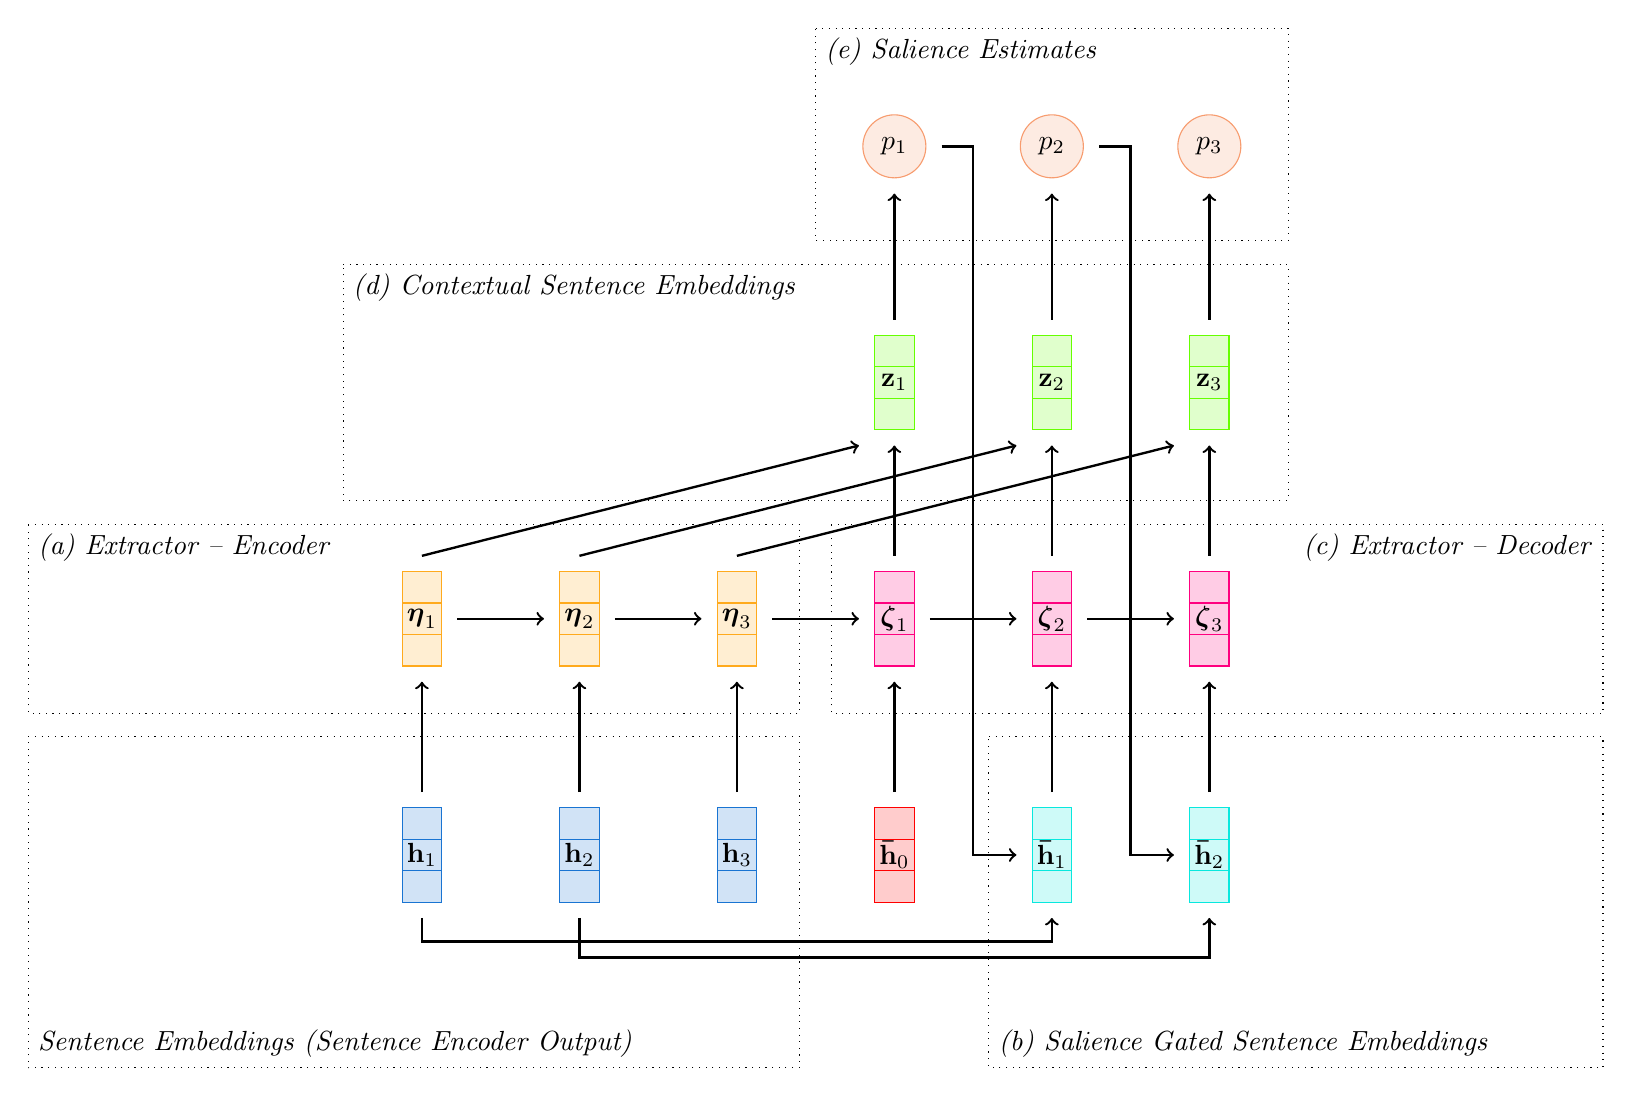
\begin{tikzpicture}[
  dep/.style ={
    ->,line width=0.3mm
  },
  hid/.style 2 args={
    rectangle split,
    draw=#2,
    rectangle split parts=#1,
    fill=#2!20,
    minimum width=5mm,
    minimum height=5mm,
    outer sep=2mm},
  mlp/.style 2 args={
    rectangle split,
    rectangle split horizontal,
    draw=#2,
    rectangle split parts=#1,
    fill=#2!20,
    outer sep=2mm},
  sal/.style={
    circle, 
    minimum width=8mm,
    outer sep=2mm,
    draw=#1, 
    fill=#1!20},
]

  \def\stepsize{2}%
  \def\lvlbase{0}%
  \def\lvlheight{3}%

    % Sentence Embeddings    
  \foreach \step in {1,...,3} {
    \node[hid={3}{sentemb}] (s\step) at (\stepsize*\step, \lvlbase) {};    
    \node at (\stepsize*\step, \lvlbase) {$\sentEmb_\step$};    
   }
    \foreach \step [count=\i from 1] in {5,6} {
        \node[hid={3}{salsentemb}] (s\step) at (\stepsize*\step, \lvlbase) {};    
        \node at (\stepsize*\step, \lvlbase) {$\salSentEmb_\i$};    
    %\draw[->] (i\step.north) -> (e\step.south);
    }

       \node[hid={3}{red}] (s4) at (\stepsize*4, \lvlbase) {};    
       \node at (\stepsize*4, \lvlbase) {$\salSentEmb_0$};    

    % RNN hidden states
    \foreach \step in {1,...,3} {
        \node[hid={3}{encemb}] (rnn_\step) 
            at (\stepsize *\step, \lvlbase + \lvlheight) {};    
        \node at (\stepsize *\step, \lvlbase + \lvlheight) {$\xEncHid_\step$}; 
    }
    \foreach \step [count=\i from 1] in {4,...,6} {
        \node[hid={3}{decemb}] (rnn_\step) 
            at (\stepsize *\step, \lvlbase + \lvlheight) {};    
        \node at (\stepsize *\step, \lvlbase + \lvlheight) {$\xDecHid_\i$}; 
    }

    \foreach \step in {1,...,6} {
        \draw[dep] (s\step.north) to (rnn_\step.south);
    }
    \foreach \start [count=\stop from 2] in {1,...,5} {
        \draw[dep] (rnn_\start.east) to (rnn_\stop.west);
    }


    \foreach \step [count=\i from 1] in {4,...,6} {
        \node[hid={3}{ctxemb}] (ctx_\i) 
            at (\stepsize *\step, \lvlbase + 2*\lvlheight) {};    
        \node at (\stepsize *\step, \lvlbase + 2*\lvlheight) {$\xPredHid_\i$}; 
        \draw[dep] (rnn_\step.north) to (ctx_\i.south);
        \draw[dep] (rnn_\i.north) to (ctx_\i.south west);
        \node[sal={sal}] (sal_\i) at (\stepsize * \step,\lvlbase + 3*\lvlheight) {};
        \node at (\stepsize * \step,\lvlbase + 3*\lvlheight) {$\psal_\i$};
        \draw[dep] (ctx_\i.north) to (sal_\i.south);
    }

    \foreach \step [count=\i from 1] in {5,...,6} {
        \draw[dep] (sal_\i) -- (\stepsize * \step - \stepsize / 2,
                            \lvlbase + 3*\lvlheight) 
                     -- (\stepsize * \step - \stepsize / 2,
                            \lvlbase + 0* \lvlheight) -> (s\step) ;

    }
    \draw[dep] (s1.south) -- ($ (s1.south) + (0,-0.3)$) --($ (s5.south) + (0,-0.3)$) -- (s5.south);

    \draw[dep] (s2.south) -- ($ (s2.south) + (0,-0.5)$) --($ (s6.south) + (0,-0.5)$) -- (s6.south);

    \draw[rectangle,draw=black,dotted] 
        (\stepsize * 3.5,\lvlbase + 3.5*\lvlheight) -- 
        (\stepsize*6.5, \lvlbase + 3.5*\lvlheight) -- 
        (\stepsize*6.5, \lvlbase + 2.6*\lvlheight) --
        (\stepsize*3.5, \lvlbase + 2.6*\lvlheight) --
        (\stepsize*3.5, \lvlbase + 3.5*\lvlheight) ;

    \node[align=left,anchor=north west] 
        at (\stepsize * 3.5,\lvlbase + 3.5*\lvlheight) 
        {\textit{(e) Salience Estimates}};

    \draw[rectangle,draw=black,dotted] 
        (\stepsize*0.5,\lvlbase + 2.5*\lvlheight) -- 
        (\stepsize*6.5, \lvlbase + 2.5*\lvlheight) -- 
        (\stepsize*6.5, \lvlbase + 1.5*\lvlheight) --
        (\stepsize*0.5, \lvlbase + 1.5*\lvlheight) --
        (\stepsize*0.5, \lvlbase + 2.5*\lvlheight) ;

    \node[align=left,anchor=north west] 
        at (\stepsize * 0.5,\lvlbase + 2.5*\lvlheight) 
        {\textit{(d) Contextual Sentence Embeddings}};

    \draw[rectangle,draw=black,dotted] 
        (\stepsize*-1.5,\lvlbase + 0.5*\lvlheight) -- 
        (\stepsize*3.4, \lvlbase + 0.5*\lvlheight) -- 
        (\stepsize*3.4, \lvlbase + -0.9*\lvlheight) --
        (\stepsize*-1.5, \lvlbase + -0.9*\lvlheight) --
        (\stepsize*-1.5, \lvlbase + 0.5*\lvlheight) ;

    \node[align=left,anchor=south west] 
        at (\stepsize * -1.5,\lvlbase + -0.9*\lvlheight) 
        {\textit{Sentence Embeddings (Sentence Encoder Output)}};

    \draw[rectangle,draw=black,dotted] 
        (\stepsize*-1.5,\lvlbase + 1.4*\lvlheight) -- 
        (\stepsize*3.4, \lvlbase + 1.4*\lvlheight) -- 
        (\stepsize*3.4, \lvlbase + 0.6*\lvlheight) --
        (\stepsize*-1.5, \lvlbase + 0.6*\lvlheight) --
        (\stepsize*-1.5, \lvlbase + 1.4*\lvlheight) ;

    \node[align=left,anchor=north west] 
        at (\stepsize * -1.5,\lvlbase + 1.4*\lvlheight) 
        {\textit{(a) Extractor -- Encoder}};

    \draw[rectangle,draw=black,dotted] 
        (\stepsize*3.6,\lvlbase + 1.4*\lvlheight) -- 
        (\stepsize*8.5, \lvlbase + 1.4*\lvlheight) -- 
        (\stepsize*8.5, \lvlbase + 0.6*\lvlheight) --
        (\stepsize*3.6, \lvlbase + 0.6*\lvlheight) --
        (\stepsize*3.6, \lvlbase + 1.4*\lvlheight) ;

    \node[align=left,anchor=north east] 
        at (\stepsize * 8.5,\lvlbase + 1.4*\lvlheight) 
        {\textit{(c) Extractor -- Decoder}};

    \draw[rectangle,draw=black,dotted] 
        (\stepsize*4.6,\lvlbase + 0.5*\lvlheight) -- 
        (\stepsize*8.5, \lvlbase + 0.5*\lvlheight) -- 
        (\stepsize*8.5, \lvlbase + -0.9*\lvlheight) --
        (\stepsize*4.6, \lvlbase + -0.9*\lvlheight) --
        (\stepsize*4.6, \lvlbase + 0.5*\lvlheight) ;

    \node[align=left,anchor=south west] 
        at (\stepsize * 4.6,\lvlbase + -0.9*\lvlheight) 
        {\textit{(b) Salience Gated Sentence Embeddings}};

\end{tikzpicture}
}}

\caption{Schematic for the \clext~sentence extractor.}
\label{fig:clext} 
\end{figure}


\subsubsection{\clext~Extractor}

The \clext~extractor \citep{cheng2016neural} is built around a somewhat
idiosyncratic \unidirectional~\sequencetosequence~model. A schematic outlining
the structure of the encoder and closely following the subsequent equations can
be found in \autoref{fig:clext}.

The encoder is fairly standard. The initial state is initialized to a zero
embedding, $\zeroEmb$, and each sentence embedding $\sentEmb_i$ is fed into the
encoder, to obtain the final encoder hidden state $\xEncHid_\docSize \in
\reals^\xhidSize$. That is,\\

%\noindent\fcolorbox{encemb}{encemb!20!}{\textit{(\hyperref[fig:clext]{Figure~\ref{fig:clext}.a}) Extractor -- Encoder}}\\[-40pt]
\noindent{\textit{(\hyperref[fig:clext]{Figure~\ref{fig:clext}.a}) Extractor -- Encoder}}\\[-40pt]
\begin{align}
    \xEncHid_0 & = \zeroEmb \\
    \xEncHid_i &= \fgru(\sentEmb_i, \xEncHid_{i-1};\clEncParams) & 
    \forall i : i \in \{1,\ldots,\docSize\}. 
\end{align}

The initial decoder hidden state $\xDecHid_0 \in \reals^{\xhidSize}$ is
initialized with the last encoder hidden state, $\xEncHid_\docSize$.  The
inputs to decoder step $i$, for $i >1$, are the salience gated
$(i-1)^\textrm{th}$ sentence embeddings,\\

%\noindent\fcolorbox{salsentemb}{salsentemb!20!}{\textit{(\hyperref[fig:clext]{Figure~\ref{fig:clext}.b}) Salience Gated Sentence Embeddings}}\\[-40pt]
\noindent{\textit{(\hyperref[fig:clext]{Figure~\ref{fig:clext}.b}) Salience Gated Sentence Embeddings}}\\[-40pt]
\begin{align}
    \salSentEmb_{i-1} & = \nnpsal_{i-1}\sentEmb_{i-1} &
    \forall i: i \in \{2,\dots,\docSize\},
\end{align}
where the salience gate is $\nnpsal_i =
\nnmodel(\nnsal_i|\nnsal_1,\ldots,\nnsal_{i-1},
\sentEmb_1,\ldots,\sentEmb_\docSize;\xParams)$, is the salience estimate
computed for sentence $\sent_{i-1}$.  For the first decoder step (i.e. $i=1$),
since there is no $\nnpsal_0$, $\salSentEmb_0$ is a special learned parameter.

The extractor decoder outputs are then computed as,\\

%\noindent\fcolorbox{decemb}{decemb!20!}{\textit{(\hyperref[fig:clext]{Figure~\ref{fig:clext}.c}) Extractor -- Decoder}}\\[-40pt]
\noindent{\textit{(\hyperref[fig:clext]{Figure~\ref{fig:clext}.c}) Extractor -- Decoder}}\\[-40pt]
\begin{align}
    \xDecHid_0  &= \xEncHid_\docSize  \\
   \xDecHid_i &= \fgru(\salSentEmb_{i-1}, \xDecHid_{i-1};\clDecParams)
   &  
    \forall i : i \in \{1,\ldots,\docSize\}  \label{eq:cl1} 
\end{align}
Note in \autoref{eq:cl1} that the decoder side \gru~input is the sentence
embedding from the previous time step, $\sentEmb_{i-1}$, weighted by its
probability of extraction, $\nnpsal_{i-1}$, from the previous step, inducing
dependence of each output $\nnsal_i$ on all previous outputs
$\nnsal_1,\ldots,\nnsal_{i-1}$.

The contextual sentence embeddings $\xPredHid_i$ are then computed by
concatenating the encoder and decoder outputs $\xEncHid_i$ and $\xDecHid_i$ and
running them through a \feedforward~layer with $\relu$ activation,\\

%\noindent\fcolorbox{ctxemb}{ctxemb!20!}{\textit{(\hyperref[fig:clext]{Figure~\ref{fig:clext}.d}) Contextual Sentence Embeddings}}\\[-30pt]
\noindent{\textit{(\hyperref[fig:clext]{Figure~\ref{fig:clext}.d}) Contextual Sentence Embeddings}}\\[-30pt]
\begin{align}
\xPredHid_i &= \relu\left(\xpWeight^{(1)} \left[\begin{array}{c}\xEncHid_i \\ \xDecHid_i \end{array}\right] + \xpBias^{(1)} \right) & 
    \forall i : i \in \{1,\ldots,\docSize\}.
\end{align}

The actual salience estimate for sentence $\sent_i$ is then computed by feeding
$\xPredHid_i$ through another \feedforward~layer with logistic sigmoid
activation,\\

%\noindent\fcolorbox{sal}{sal!20!}{\textit{(\hyperref[fig:clext]{Figure~\ref{fig:clext}.e}) Salience Estimates}}\\[-40pt]
\noindent{\textit{(\hyperref[fig:clext]{Figure~\ref{fig:clext}.e}) Salience Estimates}}\\[-40pt]
\begin{align}
 p_i = \model(\bsal_i =1|\bsal_1,\ldots,\bsal_{i-1}, \sentEmb_1,\ldots,\sentEmb_\docSize; \xParams) &= \sigma\left(\xpWeight^{(2)}\xPredHid_i + \xpBias^{(2)}  \right) & 
    \forall i : i \in \{1,\ldots,\docSize\}. 
\end{align}

The contextual embedding and salience estimate layers have parameters are
$\xpWeight^{(1)} \in \reals^{\xpHidSize \times 2 \xhidSize}$, $\xpBias^{(1)}
\in \reals^{\xpHidSize}$, $\xpWeight^{(2)} \in \reals^{1 \times \xpHidSize}$,
and $\xpBias^{(2)}\in \reals$.  The entire set of learned parameters for the
\clext~extractor are
\[
    \chi = \left\{ 
    \clEncParams, \clDecParams,
    \salSentEmb_0,
    \xpWeight^{(1)}, \xpBias^{(1)}, \xpWeight^{(2)}, \xpBias^{(2)}\right\}.
\]
The hidden layer dimensionality of the \gru~and the contextual embedding layer
is $\xhidSize = 300$ and $\xpHidSize=100$, respectively.  Dropout with drop
probability $0.25$ is applied to the \gru~outputs ($\xEncHid_i$ and
$\xDecHid_i$),   and to $\xPredHid_i$.

\subsubsection{\srext~Extractor}

\citet{nallapati2017summarunner} proposed a sentence extractor, which we refer
to as the \srext~Extractor, that factorizes the salience estimates for each
sentence into contributions from five different sources, which we refer to as
\saliencefactors.  The \saliencefactors~take into account interactions between
contextual sentence embeddings and document embeddings or summary embeddings,
as well as sentence position embeddings. Salience estimates are made
sequentially, starting with the first sentence $\sent_1$ and preceding to the
last $\sent_\docSize$. When computing the salience estimate of sentence
$\sent_i$, the previous $i-1$ salience estimates are used to update the summary
representation.

In order to construct the contextual sentence embeddings, document embeddings,
and summary embeddings, the \srext~extractor first runs a
\bidirectional~\gru~over the sentence embeddings created by the sentence
encoder (visually depicted in \autoref{fig:sr1}),\\

\begin{figure}[h!]
    \fbox{\begin{minipage}{\textwidth}
\center
\scalebox{0.75}{
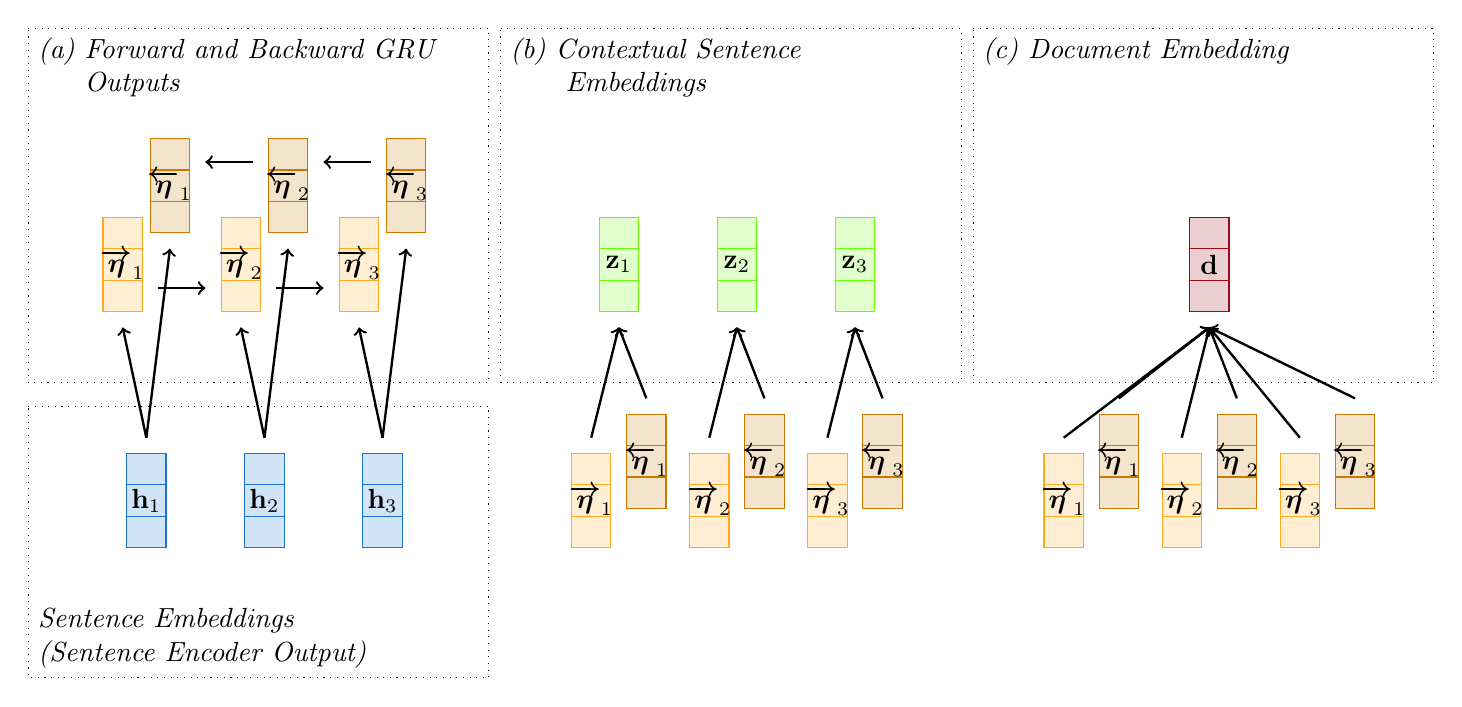
\begin{tikzpicture}[
  dep/.style ={
    ->,line width=0.3mm
  },
  hid/.style 2 args={
    rectangle split,
    draw=#2,
    rectangle split parts=#1,
    fill=#2!20,
    minimum width=5mm,
    minimum height=5mm,
    outer sep=2mm},
  mlp/.style 2 args={
    rectangle split,
    rectangle split horizontal,
    draw=#2,
    rectangle split parts=#1,
    fill=#2!20,
    outer sep=2mm},
  sal/.style={
    circle, 
    minimum width=8mm,
    outer sep=2mm,
    draw=#1, 
    fill=#1!20},
]

  \def\stepsize{1.5}%
  \def\lvlbase{0}%
  \def\lvlheight{3}%
 

    % Sentence Embeddings    
  \foreach \step in {1,...,3} {
    \node[hid={3}{sentemb}] (s\step) at (\stepsize*\step, \lvlbase) {};    
    \node at (\stepsize*\step, \lvlbase) {$\sentEmb_\step$};    
   }
    \draw[rectangle,draw=black,dotted] 
        (\stepsize*0.0,\lvlbase + 2*\lvlheight) -- 
        (\stepsize*3.9, \lvlbase + 2*\lvlheight) -- 
        (\stepsize*3.9, \lvlbase + 0.5*\lvlheight) --
        (\stepsize*0.0, \lvlbase + 0.5*\lvlheight) --
        (\stepsize*0.0, \lvlbase + 2*\lvlheight) ;

    \node[align=left,anchor=north west] 
        at (\stepsize * 0.0,\lvlbase + 2*\lvlheight) 
        {\textit{(a) Forward and Backward \gru}\\\textit{\phantom{(a) }Outputs}};

    \draw[rectangle,draw=black,dotted] 
        (\stepsize*0.0,\lvlbase + 0.4*\lvlheight) -- 
        (\stepsize*3.9, \lvlbase + 0.4*\lvlheight) -- 
        (\stepsize*3.9, \lvlbase -0.75*\lvlheight) --
        (\stepsize*0.0, \lvlbase -0.75*\lvlheight) --
        (\stepsize*0.0, \lvlbase + 0.4*\lvlheight) ;

    \node[align=left,anchor=south west] 
        at (\stepsize * 0.0,\lvlbase + -0.75*\lvlheight) 
        {\textit{Sentence Embeddings}\\\textit{(Sentence Encoder Output)}};


    \draw[rectangle,draw=black,dotted] 
        (\stepsize*4.0,\lvlbase + 2*\lvlheight) -- 
        (\stepsize*7.9, \lvlbase + 2*\lvlheight) -- 
        (\stepsize*7.9, \lvlbase + 0.5*\lvlheight) --
        (\stepsize*4.0, \lvlbase + 0.5*\lvlheight) --
        (\stepsize*4.0, \lvlbase + 2*\lvlheight) ;

    \node[align=left,anchor=north west] 
        at (\stepsize * 4.0,\lvlbase + 2*\lvlheight) 
        {\textit{(b) Contextual Sentence}\\ \textit{\phantom{(b) } Embeddings}};

    \draw[rectangle,draw=black,dotted] 
        (\stepsize*8.0,\lvlbase + 2*\lvlheight) -- 
        (\stepsize*11.9, \lvlbase + 2*\lvlheight) -- 
        (\stepsize*11.9, \lvlbase + 0.5*\lvlheight) --
        (\stepsize*8.0, \lvlbase + 0.5*\lvlheight) --
        (\stepsize*8.0, \lvlbase + 2*\lvlheight) ;

    \node[align=left,anchor=north west] 
        at (\stepsize * 8.0,\lvlbase + 2*\lvlheight) 
        {\textit{(c) Document Embedding}};




%    % RNN hidden states
    \foreach \step in {1,...,3} {
        \node[hid={3}{rencemb}] (rrnn_\step) 
            at (\stepsize *\step-0.3, \lvlbase + \lvlheight) {};    
        \node at (\stepsize *\step-0.3, \lvlbase + \lvlheight) 
            {$\rnnextRHid_\step$}; 
        \node[hid={3}{lencemb}] (lrnn_\step) 
            at (\stepsize *\step+0.3, \lvlbase + \lvlheight + 1.0) {};    
        \node at (\stepsize *\step+0.3, \lvlbase + \lvlheight+ 1.0) 
            {$\rnnextLHid_\step$}; 
        \draw[dep] (s\step.north) -- (rrnn_\step.south);
        \draw[dep] (s\step.north) -- (lrnn_\step.south);

    }
    \foreach \start [count=\stop from 2] in {1,...,2} {
        \draw[dep] ($ (rrnn_\start.east) - (0,0.3)$) 
            -- ($ (rrnn_\stop.west) - (0,0.3) $);
        \draw[dep] ($(lrnn_\stop.west) + (0,0.3)$) 
            -- ($ (lrnn_\start.east) + (0,0.3)   $);
    }

  \def\stepsize{1.5}%
  \def\lvlbase{0}%
  \def\lvlheight{3}%
 

    \foreach \step in {1,...,3} {
        \node[hid={3}{rencemb}] (rrnn_\step) 
            at (\stepsize *\step-0.35 + 5 + 1, \lvlbase + 0*\lvlheight) {};    
        \node at (\stepsize*\step-0.35 + 5 + 1, \lvlbase + 0*\lvlheight) 
            {$\rnnextRHid_\step$}; 
        \node[hid={3}{lencemb}] (lrnn_\step) 
            at (\stepsize *\step+5.35 + 1, \lvlbase + 0*\lvlheight + 0.5) {};    
        \node at (\stepsize *\step+5.35 + 1, \lvlbase + 0*\lvlheight+ 0.5) 
            {$\rnnextLHid_\step$}; 
        \node[hid={3}{ctxemb}] (ctx_\step) 
            at (\stepsize *\step + 5 + 1, \lvlbase + 1*\lvlheight) {};    
        \node at (\stepsize*\step + 5 + 1, \lvlbase + 1*\lvlheight) 
            {$\srHid_\step$}; 

        \draw[dep] (rrnn_\step.north) to (ctx_\step.south);
        \draw[dep] (lrnn_\step.north) to (ctx_\step.south);
    }


        \node[hid={3}{doc}] (doc) 
            at (\stepsize *2 + 10+2, \lvlbase + 1*\lvlheight) {};    
        \node at (\stepsize*2 + 10+2, \lvlbase + 1*\lvlheight) 
            {$\srDocEmb$}; 



    \foreach \step in {1,...,3} {
        \node[hid={3}{rencemb}] (rrnn_\step) 
            at (\stepsize *\step-0.35 + 10 + 2, \lvlbase + 0*\lvlheight) {};    
        \node at (\stepsize*\step-0.35 + 10 + 2, \lvlbase + 0*\lvlheight) 
            {$\rnnextRHid_\step$}; 
        \node[hid={3}{lencemb}] (lrnn_\step) 
            at (\stepsize *\step+10.35+2, \lvlbase + 0*\lvlheight + 0.5) {};    
        \node at (\stepsize *\step+10.35+2, \lvlbase + 0*\lvlheight+ 0.5) 
            {$\rnnextLHid_\step$}; 

        \draw[dep] (rrnn_\step.north) to (doc.south);
        \draw[dep] (lrnn_\step.north) to (doc.south);
    }


\end{tikzpicture}}


\caption{\srext~contextual sentence embedding and document embeddings.}
\label{fig:sr1}\end{minipage}}
\end{figure}


%\noindent\fcolorbox{rencemb}{rencemb!20!}{\textit{(\hyperref[fig:sr1]{Figure~\ref{fig:sr1}.a}) Forward and Backward \gru~Outputs}}\\[-40pt]
\noindent{\textit{(\hyperref[fig:sr1]{Figure~\ref{fig:sr1}.a}) Forward and Backward \gru~Outputs}}\\[-40pt]
\begin{align}
    \srrHid_0 &= \zeroEmb, \\
    \srrHid_i &= \fgru(\sentEmb_i, \srrHid_{i-1}; \srRRNNParams) &
    \forall i : i \in \{1,\ldots,\docSize\},\\
    \srlHid_{\docSize + 1} &= \zeroEmb,\\
    \srlHid_i &= \fgru(\sentEmb_i, \srlHid_{i+1}; \srLRNNParams)
    & \forall i : i \in \{1,\ldots,\docSize\},
\end{align}
where $\srrHid_i,\srlHid_i \in \reals^{\srRNNDim}$ and $\srRRNNParams$ and
$\srLRNNParams$ are the forward and backward \gru~parameters respectively.

The \gru~output is concatenated and run through a feed-forward layer to obtain
a contextual sentence embedding representation $\srHid_i \in
\reals^{\srRepDim}$,\\

%\noindent\fcolorbox{ctxemb}{ctxemb!20!}{\textit{(\hyperref[fig:sr1]{Figure~\ref{fig:sr1}.b}) Contextual Sentence Embeddings}} 
\noindent{\textit{(\hyperref[fig:sr1]{Figure~\ref{fig:sr1}.b}) Contextual Sentence Embeddings}} 
\begin{align}
\srHid_i  & = \relu\left(\srSentBias + \srSentWeight \left[ \begin{array}{c} \srrHid_i \\ \srlHid_i  \end{array} \right]  \right) &
    \forall i : i \in \{1,\ldots,\docSize\},
\end{align}
where $\srSentWeight \in \reals^{\srRepDim \times 2\srRNNDim}$ and $\srSentBias
\in \reals^{\srRepDim}$ are learned parameters.

To construct the document embedding $\srDocEmb$, the forward and backward
\gru~outputs are concatenated and averaged before running through a different
\feedforward~layer,\\

%\noindent\fcolorbox{doc}{doc!20!}{\textit{(\hyperref[fig:sr1]{Figure~\ref{fig:sr1}.c}) Document Embedding}}\\[-40pt]
\noindent{\textit{(\hyperref[fig:sr1]{Figure~\ref{fig:sr1}.c}) Document Embedding}}\\[-40pt]
\begin{align}
\srDocEmb  & = \tanh\left(\srDocBias + \srDocWeight \left(\frac{1}{\docSize}\sum_{i=1}^{\docSize} \left[ \begin{array}{c} \srrHid_i \\ \srlHid_i  \end{array} \right] \right) \right)
\end{align}
where $\srDocWeight \in \reals^{\srRepDim \times 2\srRNNDim}$ and $\srDocBias
\in \reals^{\srRepDim}$ are learned parameters.

Additionally, an iterative representation of the extract summary at step $i$,
$\srSum_i$, is constructed by summing the $i-1$ contextual sentence embeddings
weighted by their salience estimates,\\

%\noindent\fcolorbox{sum}{sum!20!}{\textit{(\autoref{fig:sr2}) Summary Embeddings}}\\[-40pt]
\noindent{\textit{(\autoref{fig:sr2}) Summary Embeddings}}\\[-40pt]
\begin{align}
\srSum_1 & = \zeroEmb, \\
\srSum_i & = \tanh\left(\sum_{j=1}^{i-1} \nnpsal_j \cdot \srHid_j\right)
& \forall i: i \in \{2,\ldots,\docSize-1 \},
\end{align}
where $\nnpsal_j=
\nnmodel\left(\nnsal_j=1|\nnsal_1,\ldots,\nnsal_{j-1},\sentEmb_1, \ldots,
\sentEmb_\docSize; \xParams\right)$ are previously computed salience estimates
for sentences $\sent_1,\ldots,\sent_{i-1}$.

\begin{figure}[t]
    \fbox{\begin{minipage}{\textwidth}
\center
\scalebox{0.75}{
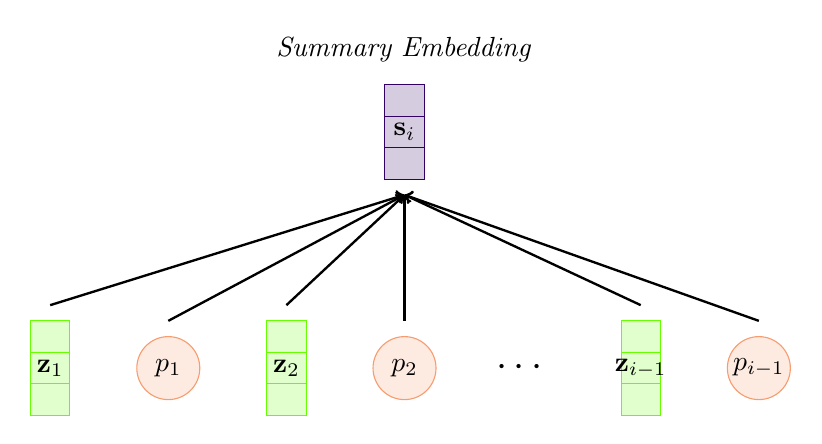
\begin{tikzpicture}[
  dep/.style ={
    ->,line width=0.3mm
  },
  hid/.style 2 args={
    rectangle split,
    draw=#2,
    rectangle split parts=#1,
    fill=#2!20,
    minimum width=5mm,
    minimum height=5mm,
    outer sep=2mm},
  mlp/.style 2 args={
    rectangle split,
    rectangle split horizontal,
    draw=#2,
    rectangle split parts=#1,
    fill=#2!20,
    outer sep=2mm},
  sal/.style={
    circle, 
    minimum width=8mm,
    outer sep=2mm,
    draw=#1, 
    fill=#1!20},
]

  \def\stepsize{1.5}%
  \def\lvlbase{0}%
  \def\lvlheight{3}%
 
  \def\stepsize{1.5}%
  \def\lvlbase{0}%
  \def\lvlheight{3}%


        \node[hid={3}{ctxemb}] (ctx_1) 
            at (\stepsize *6 , \lvlbase + -5*\lvlheight) {};    
        \node at (\stepsize*6, \lvlbase + -5*\lvlheight) 
            {$\srHid_1$}; 

        \node[sal={sal}] (p_1) 
            at (\stepsize *7 , \lvlbase + -5*\lvlheight) {};    
        \node at (\stepsize*7, \lvlbase + -5*\lvlheight) 
            {$\psal_1$}; 

        \node[hid={3}{ctxemb}] (ctx_2) 
            at (\stepsize *8 , \lvlbase + -5*\lvlheight) {};    
        \node at (\stepsize*8, \lvlbase + -5*\lvlheight) 
            {$\srHid_2$}; 

        \node[sal={sal}] (p_2) 
            at (\stepsize *9 , \lvlbase + -5*\lvlheight) {};    
        \node at (\stepsize*9, \lvlbase + -5*\lvlheight) 
            {$\psal_2$}; 


        \node[hid={3}{sum}] (summary_3) 
            at (\stepsize *9 , \lvlbase + -4*\lvlheight) {};    
        \node at (\stepsize*9, \lvlbase + -4*\lvlheight) 
            {$\srSum_{i}$}; 


            \node at (\stepsize *9 , \lvlbase + -3.65*\lvlheight) {\textit{Summary Embedding}};

        \node[hid={3}{ctxemb}] (ctx_n) 
            at (\stepsize *11 , \lvlbase + -5*\lvlheight) {};    
        \node at (\stepsize*11, \lvlbase + -5*\lvlheight) 
            {$\srHid_{i-1}$}; 

        \node[sal={sal}] (p_n) 
            at (\stepsize *12 , \lvlbase + -5*\lvlheight) {};    
        \node at (\stepsize*12, \lvlbase + -5*\lvlheight) 
            {$\psal_{i-1}$}; 

        \node at (\stepsize*10, \lvlbase + -5*\lvlheight) {\Large $\cdots$};





        \draw[dep] (ctx_1.north) to (summary_3.south);
        \draw[dep] (p_1.north) to (summary_3.south);

        \draw[dep] (ctx_2.north) to (summary_3.south);
        \draw[dep] (p_2.north) to (summary_3.south);

        \draw[dep] (ctx_n.north) to (summary_3.south);
        \draw[dep] (p_n.north) to (summary_3.south);













%        \node[hid={3}{yellow}] (ctx_1) 
%            at (\stepsize *4 , \lvlbase + -5*\lvlheight) {};    
%        \node at (\stepsize*4, \lvlbase + -5*\lvlheight) 
%            {$\srHid_1$}; 
%        \node[hid={3}{yellow}] (ctx_2) 
%            at (\stepsize *5 , \lvlbase + -5*\lvlheight) {};    
%        \node at (\stepsize*5, \lvlbase + -5*\lvlheight) 
%            {$\srHid_2$}; 
%
%
%

%    \foreach \start [count=\stop from 2] in {1,...,2} {
%        \draw[dep] ($ (rrnn_\start.east) - (0,0.3)$) 
%            -- ($ (rrnn_\stop.west) - (0,0.3) $);
%        \draw[dep] ($(lrnn_\stop.west) + (0,0.3)$) 
%            -- ($ (lrnn_\start.east) + (0,0.3)   $);
%    }

%    \draw[rectangle,draw=black,dotted] 
%        (\stepsize*-2.5,\lvlbase + 3.5*\lvlheight) -- 
%        (\stepsize*3.5, \lvlbase + 3.5*\lvlheight) -- 
%        (\stepsize*3.5, \lvlbase + 2.7*\lvlheight) --
%        (\stepsize*-2.5, \lvlbase + 2.7*\lvlheight) --
%        (\stepsize*-2.5, \lvlbase + 3.5*\lvlheight) ;
%
%    \node[align=left,anchor=north west] 
%        at (\stepsize * -2.5,\lvlbase + 3.5*\lvlheight) 
%        {\textit{Salience Estimates}};
%
%    \draw[rectangle,draw=black,dotted] 
%        (\stepsize*-2.5,\lvlbase + 2.6*\lvlheight) -- 
%        (\stepsize*3.5, \lvlbase + 2.6*\lvlheight) -- 
%        (\stepsize*3.5, \lvlbase + 1.8*\lvlheight) --
%        (\stepsize*-2.5, \lvlbase + 1.8*\lvlheight) --
%        (\stepsize*-2.5, \lvlbase + 2.6*\lvlheight) ;
%
%    \node[align=left,anchor=north west] 
%        at (\stepsize * -2.5,\lvlbase + 2.6*\lvlheight) 
%        {\textit{Contextual Sentence Embeddings}};
%
%    \draw[rectangle,draw=black,dotted] 
%        (\stepsize*-2.5,\lvlbase + 0.5*\lvlheight) -- 
%        (\stepsize*3.5, \lvlbase + 0.5*\lvlheight) -- 
%        (\stepsize*3.5, \lvlbase + -0.50*\lvlheight) --
%        (\stepsize*-2.5, \lvlbase + -0.50*\lvlheight) --
%        (\stepsize*-2.5, \lvlbase + 0.5*\lvlheight) ;
%
%    \node[align=left,anchor=north west] 
%        at (\stepsize * -2.5,\lvlbase + 0.5*\lvlheight) 
%        {\textit{Sentence Embeddings}\\\textit{(Sentence Encoder Output)}};
%
%
%    \draw[rectangle,draw=black,dotted] 
%        (\stepsize*-2.5,\lvlbase + 1.7*\lvlheight) -- 
%        (\stepsize*3.5, \lvlbase + 1.7*\lvlheight) -- 
%        (\stepsize*3.5, \lvlbase + 0.6*\lvlheight) --
%        (\stepsize*-2.5, \lvlbase + 0.6*\lvlheight) --
%        (\stepsize*-2.5, \lvlbase + 1.7*\lvlheight) ;
%
%
%    \node[align=left,anchor=north west] 
%        at (\stepsize * -2.5,\lvlbase + 1.7*\lvlheight) 
%        {\textit{Forward and Backward Partial}\\\textit{Contexual Sentence Embeddings}};

\end{tikzpicture}}

        \caption{\srext~iterative summary embeddings.}
        \label{fig:sr2}

\end{minipage}}
\end{figure}


When computing the salience of a sentence $\nnpsal_i$, the SummaRunner model
uses the contextual sentence embedding $\xHid_i$, the document embedding
$\srDocEmb$, the summary embedding $\srSum_i$, and the document position $i$.
These representations are used to compute five different factors, which are
then summed and run through a logistic sigmoid to the salience estimate.  The
five factors are named the content factor ($\srContentFactor$), the centrality
factor ($\srSalienceFactor$),\footnote{\citet{nallapati2017summarunner} refer
to this as the salience factor, but we rename it here to avoid confusion with
the model's final predictions which we call salience estimates.} the novelty
factor ($\srNoveltyFactor$), the fine grained position factor
($\srFinePositionFactor$), and the coarse grained position factor
($\srCoarsePositionFactor$).

First, there is the content factor which is simply the dot product of the
contextual sentence embedding with a learned parameter vector,\\

%\noindent\fcolorbox{factor}{factor!20!}{\textit{(\hyperref[fig:sr3]{Figure~\ref{fig:sr3}.a}) Content Factor}}\\[-40pt]
\noindent{\textit{(\hyperref[fig:sr3]{Figure~\ref{fig:sr3}.a}) Content Factor}}\\[-40pt]
\begin{align}
    \srContentFactor_i &={\srContentWeight}^\T \srHid_i & \forall i : i \in \{1,\ldots,\docSize\}, 
\end{align}
where $\srContentWeight \in \reals^{\srRepDim}$. This term is intended to
represent contributions of the individual sentences to their salience.

The centrality factor is intended to capture a sentence's similarity to the
document embedding. This interaction computed as\\

%\noindent\fcolorbox{factor}{factor!20!}{\textit{(\hyperref[fig:sr3]{Figure~\ref{fig:sr3}.b}) Centrality Factor}}\\[-40pt]
\noindent{\textit{(\hyperref[fig:sr3]{Figure~\ref{fig:sr3}.b}) Centrality Factor}}\\[-40pt]
\begin{align}
    \srSalienceFactor_i & = \srHid_i^\T\srSalienceWeight \srDocEmb & \forall i : i \in \{1,\ldots,\docSize\}, 
\end{align}
and is mediated by a learned parameter matrix, $\srSalienceWeight \in \reals^{\srRepDim \times \srRepDim}$.

The third factor, novelty, is similarly an interaction between the contextual
sentence embedding and the $i$-th summary embedding,\\

%\noindent\fcolorbox{factor}{factor!20!}{\textit{(\hyperref[fig:sr3]{Figure~\ref{fig:sr3}.c}) Novelty Factor}}\\[-40pt]
\noindent{\textit{(\hyperref[fig:sr3]{Figure~\ref{fig:sr3}.c}) Novelty Factor}}\\[-40pt]
\begin{align}
    \srNoveltyFactor_i &= -\srHid_i^\T \srNoveltyWeight \srSum_i
    & \forall i : i \in \{1,\ldots,\docSize\},
    \label{eq:srnov} 
\end{align}
where $\srNoveltyWeight \in \reals^{\srRepDim \times \srRepDim}$ is a learned
parameter matrix. Note also this factor is multiplied by negative to indicate
that high levels of similarity between $\srHid_i$ and $\srSum_i$ should be
discouraged. 


\begin{figure}
\centering
\fbox{\begin{minipage}{\textwidth}\centering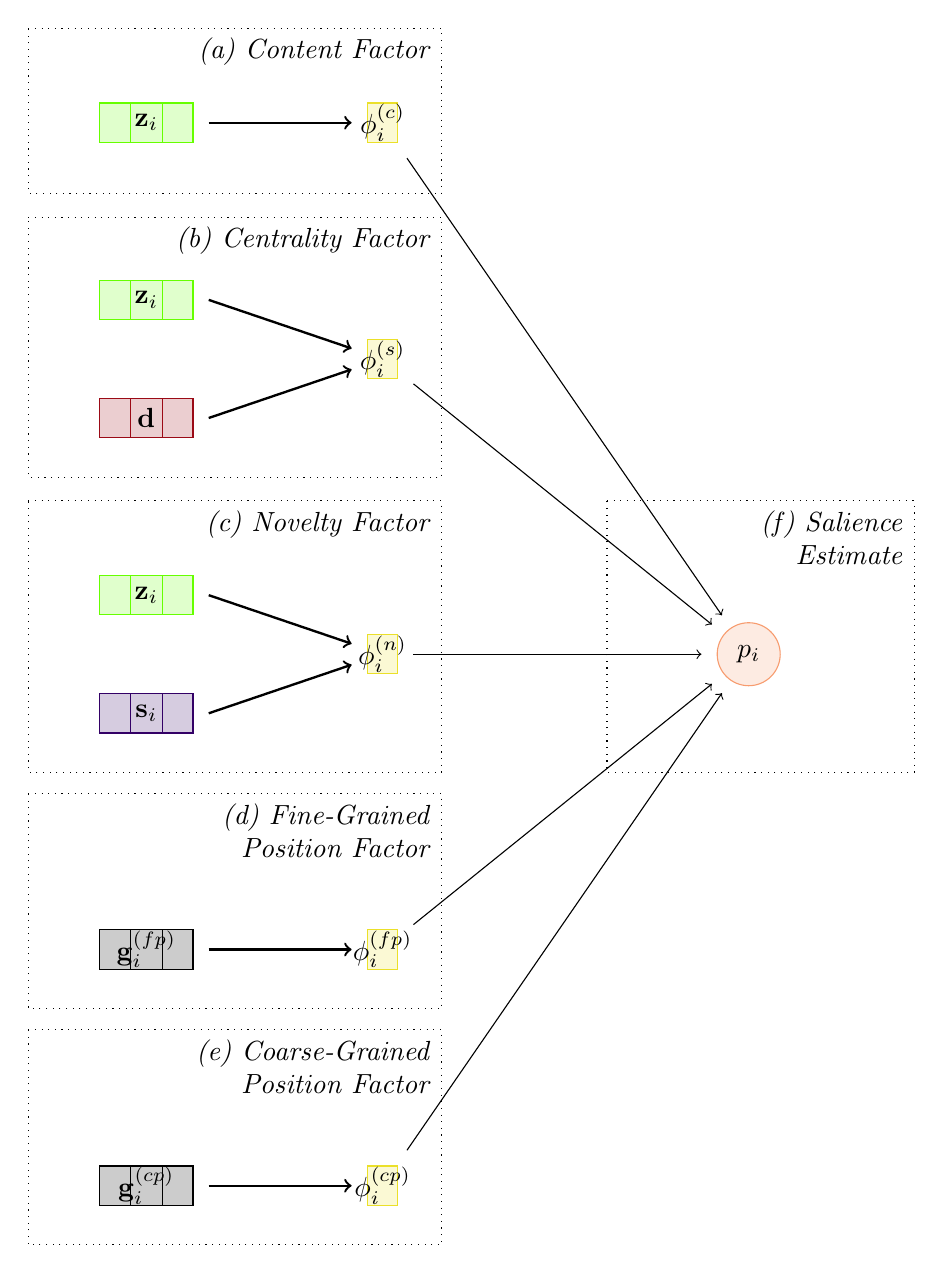
\begin{tikzpicture}[
  dep/.style ={
    ->,line width=0.3mm
  },
  hid/.style 2 args={
    rectangle split,
    rectangle split horizontal,
    draw=#2,
    rectangle split parts=#1,
    fill=#2!20,
    minimum width=5mm,
    minimum height=5mm,
    outer sep=2mm},
  mlp/.style 2 args={
    rectangle split,
    rectangle split horizontal,
    draw=#2,
    rectangle split parts=#1,
    fill=#2!20,
    outer sep=2mm},
  sal/.style={
    circle, 
    minimum width=8mm,
    outer sep=2mm,
    draw=#1, 
    fill=#1!20},
]

  \def\stepsize{3}%
  \def\lvlbase{0}%
  \def\lvlheight{3}%

   \node[sal={sal}] (sal) at (\stepsize * 3.55,\lvlbase + -4.25*\lvlheight)   {}; 
    \node at (\stepsize * 3.55,\lvlbase + -4.25*\lvlheight) {$\psal_i$}; 



        \node[hid={3}{ctxemb}] (ctx_i) 
            at (\stepsize *1 , \lvlbase + -2*\lvlheight) {};    
        \node at (\stepsize*1, \lvlbase + -2*\lvlheight) 
            {$\srHid_i$}; 

        \node[hid={1}{factor}] (content_i) 
            at (\stepsize *2, \lvlbase + -2*\lvlheight) {};    
        \node at (\stepsize*2, \lvlbase + -2*\lvlheight) 
            {$\srContentFactor_i$}; 
        \draw[->] (content_i) -- (sal);

        \draw[dep] (ctx_i) to (content_i);
    \draw[rectangle,draw=black,dotted] 
        (\stepsize*0.5,\lvlbase -1.6*\lvlheight) -- 
        (\stepsize*2.25, \lvlbase -1.6*\lvlheight) -- 
        (\stepsize*2.25, \lvlbase - 2.3*\lvlheight) --
        (\stepsize*0.5, \lvlbase -2.3*\lvlheight) --
        (\stepsize*0.5, \lvlbase -1.6*\lvlheight) ;
%

    \node[align=left,anchor=north east] 
        at (\stepsize * 2.25,\lvlbase + -1.6*\lvlheight) 
            {\textit{(a) Content Factor}};

        \node[hid={3}{ctxemb}] (ctx_i) 
            at (\stepsize *1 , \lvlbase + -2.75*\lvlheight) {};    
        \node at (\stepsize*1, \lvlbase + -2.75*\lvlheight) 
            {$\srHid_i$}; 

        \node[hid={1}{factor}] (salience_i) 
            at (\stepsize *2, \lvlbase + -3*\lvlheight) {};    
        \node at (\stepsize*2, \lvlbase + -3*\lvlheight) 
            {$\srSalienceFactor_i$}; 

        \draw[->] (salience_i) -- (sal);
        \node[hid={3}{doc}] (doc) 
            at (\stepsize *1, \lvlbase + -3.25*\lvlheight) {};    
        \node at (\stepsize*1, \lvlbase + -3.25*\lvlheight) 
            {$\srDocEmb$}; 

        \draw[dep] (ctx_i.east) to (salience_i);
        \draw[dep] (doc.east) to (salience_i);

    \draw[rectangle,draw=black,dotted] 
        (\stepsize*0.5,\lvlbase -2.4*\lvlheight) -- 
        (\stepsize*2.25, \lvlbase -2.4*\lvlheight) -- 
        (\stepsize*2.25, \lvlbase - 3.5*\lvlheight) --
        (\stepsize*0.5, \lvlbase -3.5*\lvlheight) --
        (\stepsize*0.5, \lvlbase -2.4*\lvlheight) ;

    \node[align=left,anchor=north east] 
        at (\stepsize * 2.25,\lvlbase + -2.4*\lvlheight) 
            {\textit{(b) Centrality Factor}};

        \node[hid={3}{ctxemb}] (ctx_i) 
            at (\stepsize *1 , \lvlbase + -4.0*\lvlheight) {};    
        \node at (\stepsize*1, \lvlbase + -4.0*\lvlheight) 
            {$\srHid_i$}; 

        \node[hid={1}{factor}] (salience_i) 
            at (\stepsize *2, \lvlbase + -4.25*\lvlheight) {};    
        \node at (\stepsize*2, \lvlbase + -4.25*\lvlheight) 
            {$\srNoveltyFactor_i$}; 

        \draw[->] (salience_i) -- (sal);
        \node[hid={3}{sum}] (doc) 
            at (\stepsize *1, \lvlbase + -4.5*\lvlheight) {};    
        \node at (\stepsize*1, \lvlbase + -4.5*\lvlheight) 
            {$\srSum_i$}; 

        \node[hid={3}{black}] (fg) 
            at (\stepsize *1, \lvlbase + -5.5*\lvlheight) {};    
        \node at (\stepsize*1, \lvlbase + -5.5*\lvlheight) 
            {$\srFinePositionEmb_i$}; 

        \node[hid={1}{factor}] (fine_i) 
            at (\stepsize *2, \lvlbase + -5.5*\lvlheight) {};    
        \node at (\stepsize*2, \lvlbase + -5.5*\lvlheight) 
            {$\srFinePositionFactor_i$}; 

        \draw[->] (fine_i) -- (sal);

    \node[anchor=north east,align=right] 
        at (\stepsize * 2.25,\lvlbase + -4.84*\lvlheight) 
            {\textit{(d) Fine-Grained}\\\textit{Position Factor}};

    \node[align=right,anchor=north east] 
        at (\stepsize * 2.25,\lvlbase + -5.84*\lvlheight) 
            {\textit{(e) Coarse-Grained}\\\textit{Position Factor}};


        \node[hid={3}{black}] (cg) 
            at (\stepsize *1, \lvlbase + -6.5*\lvlheight) {};    
        \node at (\stepsize*1, \lvlbase + -6.5*\lvlheight) 
            {$\srCoarsePositionEmb_i$}; 
        \node[hid={1}{factor}] (coarse_i) 
            at (\stepsize *2, \lvlbase + -6.5*\lvlheight) {};    
        \node at (\stepsize*2, \lvlbase + -6.5*\lvlheight) 
            {$\srCoarsePositionFactor_i$}; 

        \draw[->] (coarse_i) -- (sal);



        \draw[dep] (ctx_i.east) to (salience_i);
        \draw[dep] (doc.east) to (salience_i);


    \draw[rectangle,draw=black,dotted] 
        (\stepsize*0.5,\lvlbase -3.6*\lvlheight) -- 
        (\stepsize*2.25, \lvlbase -3.6*\lvlheight) -- 
        (\stepsize*2.25, \lvlbase - 4.75*\lvlheight) --
        (\stepsize*0.5, \lvlbase -4.75*\lvlheight) --
        (\stepsize*0.5, \lvlbase -3.6*\lvlheight) ;
    \draw[rectangle,draw=black,dotted] 
        (\stepsize*2.95,\lvlbase -3.6*\lvlheight) -- 
        (\stepsize*4.25, \lvlbase -3.6*\lvlheight) -- 
        (\stepsize*4.25, \lvlbase - 4.75*\lvlheight) --
        (\stepsize*2.95, \lvlbase -4.75*\lvlheight) --
        (\stepsize*2.95, \lvlbase -3.6*\lvlheight) ;


    \node[align=left,anchor=north east] 
        at (\stepsize * 2.25,\lvlbase + -3.6*\lvlheight) 
            {\textit{(c) Novelty Factor}};

    \node[align=right,anchor=north east] 
        at (\stepsize * 4.25,\lvlbase + -3.6*\lvlheight) 
            {\textit{(f) Salience}\\\textit{Estimate}};




    \draw[rectangle,draw=black,dotted] 
        (\stepsize*0.5,\lvlbase -4.84*\lvlheight) -- 
        (\stepsize*2.25, \lvlbase -4.84*\lvlheight) -- 
        (\stepsize*2.25, \lvlbase - 5.75*\lvlheight) --
        (\stepsize*0.5, \lvlbase -5.75*\lvlheight) --
        (\stepsize*0.5, \lvlbase -4.84*\lvlheight) ;

    \draw[rectangle,draw=black,dotted] 
        (\stepsize*0.5,\lvlbase -5.84*\lvlheight) -- 
        (\stepsize*2.25, \lvlbase -5.84*\lvlheight) -- 
        (\stepsize*2.25, \lvlbase - 6.75*\lvlheight) --
        (\stepsize*0.5, \lvlbase -6.75*\lvlheight) --
        (\stepsize*0.5, \lvlbase -5.84*\lvlheight) ;



        \draw[dep] (fg) to (fine_i);
        \draw[dep] (cg) to (coarse_i);



\end{tikzpicture}\end{minipage}}
\caption{Schematic of salience estimation in the SummaRunner extractor.}
\label{fig:sr3}
\end{figure}


Finally, there are two factors for the fine- and coarse-grained position,\\

%\noindent\fcolorbox{factor}{factor!20!}{\textit{(\hyperref[fig:sr3]{Figure~\ref{fig:sr3}.d}) Fine-grained Position Factor}}\\[-40pt]
\noindent{\textit{(\hyperref[fig:sr3]{Figure~\ref{fig:sr3}.d}) Fine-grained Position Factor}}\\[-40pt]
\begin{align}
    \srFinePositionFactor& = {\srFinePositionWeight}^\T \srFinePositionEmb_i
& \forall i : i \in \{1,\ldots,\docSize\}, 
\end{align}
%\noindent\fcolorbox{factor}{factor!20!}{\textit{(\hyperref[fig:sr3]{Figure~\ref{fig:sr3}.e}) Coarse-grained Position Factor}}\\[-40pt]
\noindent{\textit{(\hyperref[fig:sr3]{Figure~\ref{fig:sr3}.e}) Coarse-grained Position Factor}}\\[-40pt]
\begin{align}
    \srCoarsePositionFactor& = {\srCoarsePositionWeight}^\T \srCoarsePositionEmb_i & \forall i : i \in \{1,\ldots,\docSize\}, 
\end{align}
where $\srFinePositionEmb_i$ and $\srCoarsePositionEmb_i$ are embeddings
associated with the sentence position and sentence position quartile of the
$i$-th sentence (e.g., sentence $s_7$ in a document with 12 sentences, would
have embeddings $\srFinePositionEmb_7$ and $\srCoarsePositionEmb_2$
corresponding to the seventh sentence position and $2^\textrm{nd}$ sentence
position quartile respectively).  Both $\srFinePositionWeight,
\srCoarsePositionWeight \in \reals^{\srPosDim}$, and
$\srFinePositionEmb_1,\ldots,\srFinePositionEmb_\docSizeMax,\srCoarsePositionEmb_1,\ldots,\srCoarsePositionEmb_4
\in \reals^{\srPosDim}$ are learned parameters of the \srext~extractor, and
$\docSizeMax\in\naturals$ is the maximum document size in sentences (when
handling unusually long documents, sentences with positions greater than
$\docSizeMax$ are all mapped to $\srFinePositionEmb_\docSizeMax$).

Each salience estimate $\psal_i$ is calculated as the sum of those five
factors~run through a logistic sigmoid function,\\~\\

%\noindent\fcolorbox{sal}{sal!20!}{\textit{(\hyperref[fig:sr3]{Figure~\ref{fig:sr3}.f}) Salience Estimates}}\\[-40pt]
\noindent{\textit{(\hyperref[fig:sr3]{Figure~\ref{fig:sr3}.f}) Salience Estimates}}\\[-40pt]
\begin{align}
  \nnpsal_i =  \nnmodel(\nnsal_i=1|\nnsal_1,\dots,\nnsal_{i-1},\sentEmb_1,\ldots,\sentEmb_\docSize;\xParams)
         & = 
        \sigma\left(\srContentFactor_i 
        + \srSalienceFactor_i + \srNoveltyFactor_i
    + \srFinePositionFactor_i + \srCoarsePositionFactor_i   \right) \nonumber \\
    & \phantom{= } \quad \forall i : i \in \{1,\ldots,\docSize\}.
\end{align}
We should give a bit of caution about interpreting the individual factors along
the lines of their given names as the learning procedure does not enforce that
their actual values meaningfully correspond to their names. For example, it
could be that a sentence's similarity to the summary embedding is actually
positively correlated with high salience. In such a case, the model could learn
to produce a large negative value for $\srHid_i^\T \srNoveltyWeight \srSum_i$,
such that the ``novelty'' factor $\srNoveltyFactor_i$ now has large positive
values when the $i$-th sentence is not novel to the summary. In this sense, for
a sufficiently over-parameterized network, the negative in novelty term is
superfluous as the model can learn around it. 

The complete set of parameters for the \srext~extractor is 
\[
    \xParams = \left\{\srRRNNParams,\srLRNNParams,\srSentWeight,\srSentBias,
\srDocWeight,\srDocBias, \srContentWeight, \srSalienceWeight, \srNoveltyWeight,
\srFinePositionWeight, \srCoarsePositionWeight, \srFinePositionEmb_1,\ldots,\srFinePositionEmb_{\docSizeMax}, \srCoarsePositionEmb_1,\ldots,\srCoarsePositionEmb_4,\right\}. 
\]
In our experiments, we set $\srRNNDim=300$, $\srRNNDim=100$, and
$\srPosDim=16$. Dropout with drop probability of $0.25$ is applied to the
\gru~outputs $\srrHid_i$ and $\srlHid_i$, as well as the contextual sentence
embeddings $\srHid_i$ for all $i \in \{1,\ldots,\docSize\}$.

\subsubsection{\rnnext~Extractor}


\begin{figure}[t]
    \fbox{\begin{minipage}{\textwidth}
\center
\scalebox{0.75}{
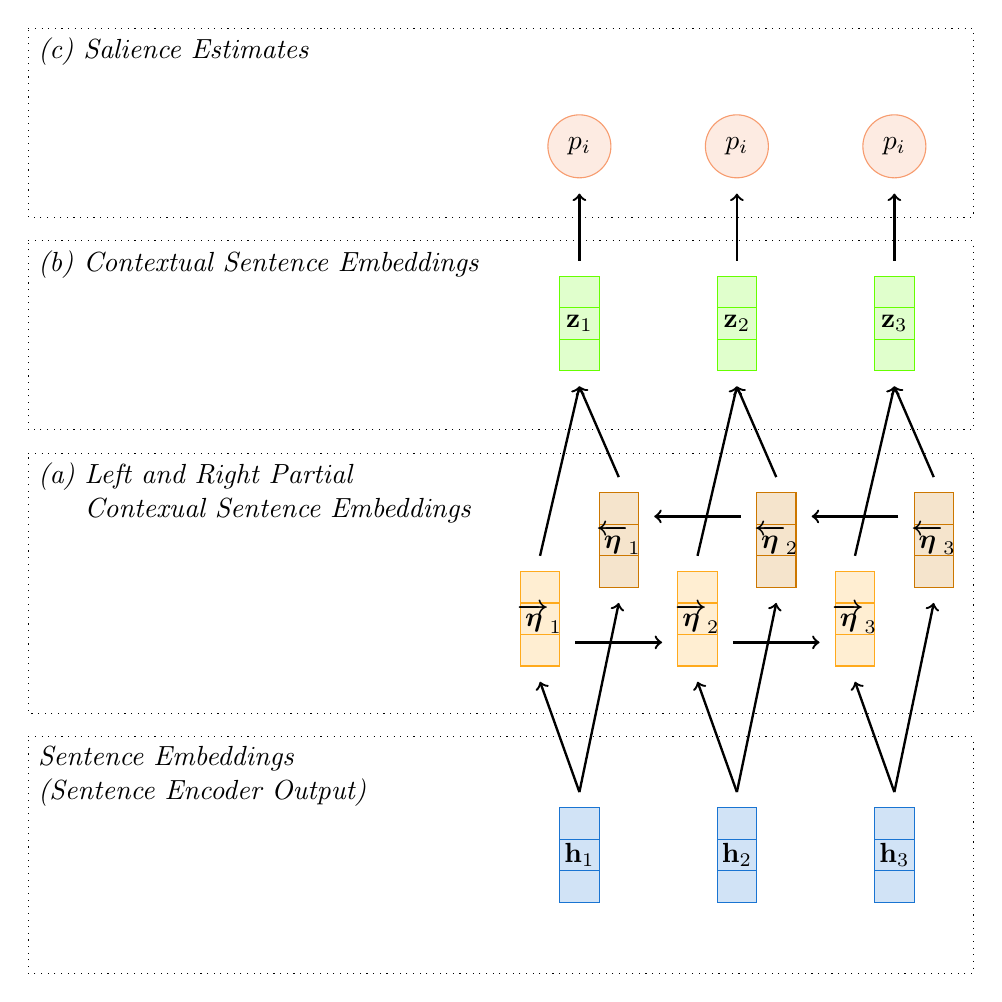
\begin{tikzpicture}[
  dep/.style ={
    ->,line width=0.3mm
  },
  hid/.style 2 args={
    rectangle split,
    draw=#2,
    rectangle split parts=#1,
    fill=#2!20,
    minimum width=5mm,
    minimum height=5mm,
    outer sep=2mm},
  mlp/.style 2 args={
    rectangle split,
    rectangle split horizontal,
    draw=#2,
    rectangle split parts=#1,
    fill=#2!20,
    outer sep=2mm},
  sal/.style={
    circle, 
    minimum width=8mm,
    outer sep=2mm,
    draw=#1, 
    fill=#1!20},
]

  \def\stepsize{2}%
  \def\lvlbase{0}%
  \def\lvlheight{3}%
 

    % Sentence Embeddings    
  \foreach \step in {1,...,3} {
    \node[hid={3}{sentemb}] (s\step) at (\stepsize*\step, \lvlbase) {};    
    \node at (\stepsize*\step, \lvlbase) {$\sentEmb_\step$};    
   }
%    \foreach \step [count=\i from 1] in {5,6} {
%        \node[hid={3}{green}] (s\step) at (\stepsize*\step, \lvlbase) {};    
%        \node at (\stepsize*\step, \lvlbase) {$\sentEmb_\i$};    
%    %\draw[->] (i\step.north) -> (e\step.south);
%    }
%
%       \node[hid={3}{red}] (s4) at (\stepsize*4, \lvlbase) {};    
%       \node at (\stepsize*4, \lvlbase) {$\sentEmb_0$};    
%
%    % RNN hidden states
    \foreach \step in {1,...,3} {
        \node[hid={3}{rencemb}] (rrnn_\step) 
            at (\stepsize *\step-0.5, \lvlbase + \lvlheight) {};    
        \node at (\stepsize *\step-0.5, \lvlbase + \lvlheight) 
            {$\rnnextRHid_\step$}; 
        \node[hid={3}{lencemb}] (lrnn_\step) 
            at (\stepsize *\step+0.5, \lvlbase + \lvlheight + 1.0) {};    
        \node at (\stepsize *\step+0.5, \lvlbase + \lvlheight+ 1.0) 
            {$\rnnextLHid_\step$}; 
        \draw[dep] (s\step.north) -- (rrnn_\step.south);
        \draw[dep] (s\step.north) -- (lrnn_\step.south);


        \node[hid={3}{ctxemb}] (ctx_\step) 
            at (\stepsize *\step, \lvlbase + 2.25*\lvlheight) {};    
        \node at (\stepsize *\step, \lvlbase + 2.25*\lvlheight) 
            {$\rnnextHid_\step$}; 
        \draw[dep] (rrnn_\step.north) -- (ctx_\step.south);
        \draw[dep] (lrnn_\step.north) -- (ctx_\step.south);


        \node[sal={sal}] (sal_\step) 
            at (\stepsize *\step, \lvlbase + 3*\lvlheight) {};    
        \node at (\stepsize *\step, \lvlbase + 3*\lvlheight) 
            {$\psal_i$}; 
        \draw[dep] (ctx_\step.north) -- (sal_\step.south);
        %\draw[dep] (lrnn_\step.north) -- (ctx_\step.south);


    }
    \foreach \start [count=\stop from 2] in {1,...,2} {
        \draw[dep] ($ (rrnn_\start.east) - (0,0.3)$) 
            -- ($ (rrnn_\stop.west) - (0,0.3) $);
        \draw[dep] ($(lrnn_\stop.west) + (0,0.3)$) 
            -- ($ (lrnn_\start.east) + (0,0.3)   $);
    }

    \draw[rectangle,draw=black,dotted] 
        (\stepsize*-2.5,\lvlbase + 3.5*\lvlheight) -- 
        (\stepsize*3.5, \lvlbase + 3.5*\lvlheight) -- 
        (\stepsize*3.5, \lvlbase + 2.7*\lvlheight) --
        (\stepsize*-2.5, \lvlbase + 2.7*\lvlheight) --
        (\stepsize*-2.5, \lvlbase + 3.5*\lvlheight) ;

    \node[align=left,anchor=north west] 
        at (\stepsize * -2.5,\lvlbase + 3.5*\lvlheight) 
        {\textit{(c) Salience Estimates}};

    \draw[rectangle,draw=black,dotted] 
        (\stepsize*-2.5,\lvlbase + 2.6*\lvlheight) -- 
        (\stepsize*3.5, \lvlbase + 2.6*\lvlheight) -- 
        (\stepsize*3.5, \lvlbase + 1.8*\lvlheight) --
        (\stepsize*-2.5, \lvlbase + 1.8*\lvlheight) --
        (\stepsize*-2.5, \lvlbase + 2.6*\lvlheight) ;

    \node[align=left,anchor=north west] 
        at (\stepsize * -2.5,\lvlbase + 2.6*\lvlheight) 
        {\textit{(b) Contextual Sentence Embeddings}};

    \draw[rectangle,draw=black,dotted] 
        (\stepsize*-2.5,\lvlbase + 0.5*\lvlheight) -- 
        (\stepsize*3.5, \lvlbase + 0.5*\lvlheight) -- 
        (\stepsize*3.5, \lvlbase + -0.50*\lvlheight) --
        (\stepsize*-2.5, \lvlbase + -0.50*\lvlheight) --
        (\stepsize*-2.5, \lvlbase + 0.5*\lvlheight) ;

    \node[align=left,anchor=north west] 
        at (\stepsize * -2.5,\lvlbase + 0.5*\lvlheight) 
        {\textit{Sentence Embeddings}\\\textit{(Sentence Encoder Output)}};


    \draw[rectangle,draw=black,dotted] 
        (\stepsize*-2.5,\lvlbase + 1.7*\lvlheight) -- 
        (\stepsize*3.5, \lvlbase + 1.7*\lvlheight) -- 
        (\stepsize*3.5, \lvlbase + 0.6*\lvlheight) --
        (\stepsize*-2.5, \lvlbase + 0.6*\lvlheight) --
        (\stepsize*-2.5, \lvlbase + 1.7*\lvlheight) ;


    \node[align=left,anchor=north west] 
        at (\stepsize * -2.5,\lvlbase + 1.7*\lvlheight) 
        {\textit{(a) Left and Right Partial}\\\textit{\phantom{(a) }Contexual Sentence Embeddings}};


\end{tikzpicture}}

\caption{Schematic for the \rnnext~sentence extractor.}
\label{fig:rnnext}
\end{minipage}}
\end{figure}


Our first proposed non-autoregressive model is a very simple
\bidirectional~\recurrentneuralnetwork~based tagging model
\citep{graves2005,wang2015}, which we refer to as the \rnnext~extractor.  See
\autoref{fig:rnnext} for a visual depiction of   the extractor.  As in the
\srext~extractor, the first step of the \rnnext~extractor is to run a
\bidirectional~\recurrentneuralnetwork~over the sentence embeddings produced by
the sentence encoder layer, which produces left and right partial contextual
embeddings $\rnnextRHid_i$ and $\rnnextLHid_i$ respectively,\\

%\noindent\fcolorbox{rencemb}{rencemb!20!}{\textit{(\hyperref[fig:rnnext]{Figure~\ref{fig:rnnext}.a}) Left and Right Partial Contexual Sentence Embeddings}}\\[-40pt]
\noindent{\textit{(\hyperref[fig:rnnext]{Figure~\ref{fig:rnnext}.a}) Left and Right Partial Contexual Sentence Embeddings}}\\[-40pt]
\begin{align}
    \rnnextRHid_0 & = \zeroEmb,\\ 
 \rnnextRHid_i &= \fgru\left(\sentEmb_i, \rnnextRHid_{i-1}; \rnnextRParams\right) &
    \forall i : i \in \{1,\ldots,\docSize\}, \\
  \rnnextLHid_{\docSize+1} & = \zeroEmb, \\
 \rnnextLHid_i &= \fgru\left(\sentEmb_i, \rnnextLHid_{i+1};\rnnextLParams\right) &
    \forall i : i \in \{\docSize, \ldots, 1\}, 
\end{align}
where $\rnnextRHid_i,\rnnextLHid_i \in \reals^{\rnnextRNNDim}$,
and $\rnnextRParams$ and $\rnnextLParams$ are the forward and backward
\gru~parameters.

The left and right partial contextual embeddings of each sentence 
are then passed through a \feedforward~layer to produce contextual
sentence embeddings $\rnnextHid_i$,\\

%\noindent\fcolorbox{ctxemb}{ctxemb!20!}{\textit{(\hyperref[fig:rnnext]{Figure~\ref{fig:rnnext}.b}) Contexual Sentence Embeddings}}\\[-35pt]
\noindent{\textit{(\hyperref[fig:rnnext]{Figure~\ref{fig:rnnext}.b}) Contexual Sentence Embeddings}}\\[-35pt]
\begin{align}
   \rnnextHid_i &= \relu\left(
    \rnnextHidWeight
    \left[ \begin{array}{c} 
        \rnnextRHid_i \\
        \rnnextLHid_i \end{array}\right] + \rnnextHidBias \right)
    & \forall i :\;\; i \in \{1,\ldots,\docSize\},
\end{align}
where $\rnnextHidWeight \in \reals^{\rnnextHidDim \times 2 \rnnextRNNDim}$
and $\rnnextHidBias \in \reals^{\rnnextHidDim}$ are learned parameters.

Another \feedforward~layer with a logistic sigmoid activation computes the
actual salience estimates $\nnpsal_1,\ldots,\nnpsal_\docSize$ where $\nnpsal_i
= \nnmodel(\nnsal_i=1|\sentEmb_1,\ldots,\sentEmb_\docSize;\xParams)$ and \\

%\noindent\fcolorbox{sal}{sal!20!}{\textit{(\hyperref[fig:rnnext]{Figure~\ref{fig:rnnext}.c}) Salience Estimates}}\\[-40pt]
\noindent{\textit{(\hyperref[fig:rnnext]{Figure~\ref{fig:rnnext}.c}) Salience Estimates}}\\[-40pt]
\begin{align}
    \nnpsal_i &= \nnmodel(\nnsal_i=1|\sentEmb_i,\ldots,\sentEmb_\docSize; \xParams) = \sigma\left(\rnnextPredWeight\rnnextHid_i + \rnnextPredBias  \right) &
    \forall i :  i \in \{1,\ldots,\docSize\},
\end{align}
where $\rnnextPredWeight \in \reals^{1 \times \rnnextHidDim}$
and $\rnnextPredBias \in \reals$ are learned parameters.

The complete set of parameters for the extractor is 
\[ \xParams = \left\{\rnnextRParams, \rnnextLParams, \rnnextHidWeight, \rnnextHidBias, \rnnextPredWeight, \rnnextPredBias \right\}.\]
In our experiments, we set $\rnnextRNNDim=300$ and $\rnnextHidDim=100$.
Dropout with drop probability of $0.25$ is applied to $\rnnextRHid_i,
\rnnextLHid_i,$ and $\rnnextHid_i$ for $i \in \{1,\ldots,\docSize\}$.

\FloatBarrier

\subsubsection{\sts~Extractor} 

One shortcoming of the RNN extractor is that long range information from one
end of the document may not easily be able to affect extraction probabilities
of sentences at the other end.  Our second proposed model, the \sts~extractor
mitigates this problem with an attention mechanism commonly used for neural
machine translation \citep{bahdanau2015,luong2015} and abstractive
summarization \citep{see2017}. The \sts~extractor has distinct encoder and
decoder bidirectional GRUs  which create distinct sequences of encoder
contextual embeddings and decoder contextual embeddings (see
\autoref{fig:stsext1} and \autoref{fig:stsext2} respectively).  Using the
attention mechanism, each decoder contextual embedding $\stsextDecHid_i$
attends to the encoder contextual embeddings,
$\stsextEncHid_1,\ldots,\stsextEncHid_\docSize$, to create the final contextual
sentence embedding $\stsextHid_i$. The final contextual embedding,
$\stsextHid_i$, thus contains a representation of sentence $\sent_i$ as well as
its relation to the other contextual representations of the remaining
sentences.  The salience estimate for $\sent_i$ is then produces by running
$\stsextHid_i$ through a feed-forward layer with logistic sigmoid output (see
\autoref{fig:stsext3}). We now describe in detail the encoder, decoder, and
attention/salience estimation layers.

The sentence embeddings produced by the sentence encoder are first encoded by a
\bidirectional~\gru, which produces left and right partial contextual sentence
embeddings, \\

\begin{figure}[t]
\fbox{\begin{minipage}{\textwidth}
\center
\scalebox{0.75}{
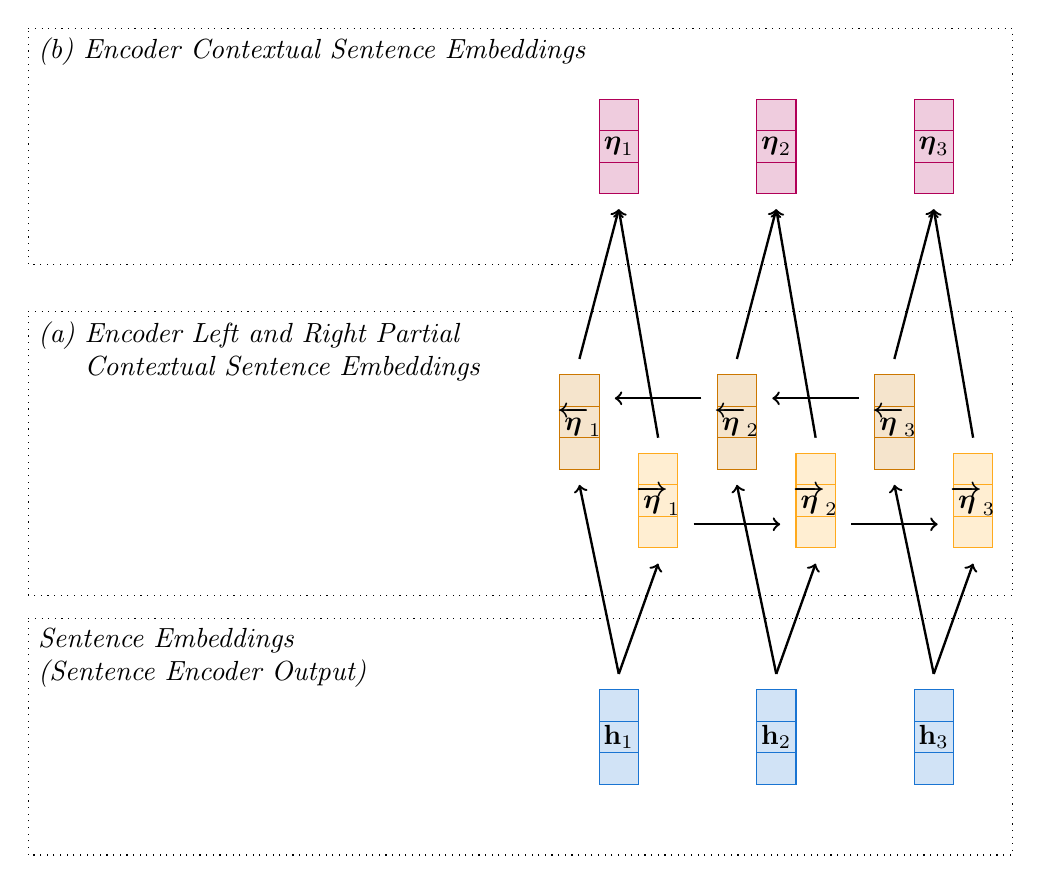
\begin{tikzpicture}[
  dep/.style ={
    ->,line width=0.3mm
  },
  hid/.style 2 args={
    rectangle split,
    draw=#2,
    rectangle split parts=#1,
    fill=#2!20,
    minimum width=5mm,
    minimum height=5mm,
    outer sep=2mm},
  mlp/.style 2 args={
    rectangle split,
    rectangle split horizontal,
    draw=#2,
    rectangle split parts=#1,
    fill=#2!20,
    outer sep=2mm},
  sal/.style={
    circle, 
    minimum width=8mm,
    outer sep=2mm,
    draw=#1, 
    fill=#1!20},
]

  \def\stepsize{2}%
  \def\lvlbase{0}%
  \def\lvlheight{3}%
 

    % Sentence Embeddings    
  \foreach \step in {1,...,3} {
    \node[hid={3}{sentemb}] (s\step) at (\stepsize*\step, \lvlbase) {};    
    \node at (\stepsize*\step, \lvlbase) {$\sentEmb_\step$};    
   }
%    \foreach \step [count=\i from 1] in {5,...,7} {
%        \node[hid={3}{green}] (s\step) at (\stepsize*\step, \lvlbase) {};    
%        \node at (\stepsize*\step, \lvlbase) {$\sentEmb_\i$};    
%    %\draw[->] (i\step.north) -> (e\step.south);
%    }

%       \node[hid={3}{red}] (s4) at (\stepsize*4, \lvlbase) {};    
%       \node at (\stepsize*4, \lvlbase) {$\sentEmb_0$};    
%
%    % RNN hidden states
    \foreach \step in {1,...,3} {
        \node[hid={3}{rencemb}] (rrnn_\step) 
            at (\stepsize *\step+0.5, \lvlbase + \lvlheight) {};    
        \node at (\stepsize *\step+0.5, \lvlbase + \lvlheight) 
            {$\stsextREncHid_\step$}; 

        \node[hid={3}{lencemb}] (lrnn_\step) 
            at (\stepsize *\step-0.5, \lvlbase + \lvlheight+1.0) {};    
        \node at (\stepsize *\step-0.5, \lvlbase + \lvlheight+1.0) 
            {$\stsextLEncHid_\step$}; 


        \node[hid={3}{encctxemb}] (enc_ctx_\step) 
            at (\stepsize *\step, \lvlbase + 2.5*\lvlheight) {};    
        \node at (\stepsize *\step, \lvlbase + 2.5*\lvlheight) 
            {$\stsextEncHid_\step$}; 

        \draw[dep] (s\step.north) -- (lrnn_\step.south);
        \draw[dep] (s\step.north) -- (rrnn_\step.south);

        \draw[dep] (lrnn_\step.north) -- (enc_ctx_\step.south);
        \draw[dep] (rrnn_\step.north) -- (enc_ctx_\step.south);
    }
    \foreach \start [count=\stop from 2] in {1,...,2} {
        \draw[dep] ($ (rrnn_\start.east) - (0,0.3)$) 
            -- ($ (rrnn_\stop.west) - (0,0.3) $);
        \draw[dep] ($(lrnn_\stop.west) + (0,0.3)$) 
            -- ($ (lrnn_\start.east) + (0,0.3)   $);
    }


    \draw[rectangle,draw=black,dotted] 
        (\stepsize*-2.75,\lvlbase + 0.5*\lvlheight) -- 
        (\stepsize*3.5, \lvlbase + 0.5*\lvlheight) -- 
        (\stepsize*3.5, \lvlbase + -0.50*\lvlheight) --
        (\stepsize*-2.75, \lvlbase + -0.50*\lvlheight) --
        (\stepsize*-2.75, \lvlbase + 0.5*\lvlheight) ;

    \node[align=left,anchor=north west] 
        at (\stepsize * -2.75,\lvlbase + 0.5*\lvlheight) 
        {\textit{Sentence Embeddings}\\\textit{(Sentence Encoder Output)}};

    \draw[rectangle,draw=black,dotted] 
        (\stepsize*-2.75,\lvlbase + 3.0*\lvlheight) -- 
        (\stepsize*3.5, \lvlbase + 3.0*\lvlheight) -- 
        (\stepsize*3.5, \lvlbase + 2.0*\lvlheight) --
        (\stepsize*-2.75, \lvlbase + 2.0*\lvlheight) --
        (\stepsize*-2.75, \lvlbase + 3.0*\lvlheight) ;

    \node[align=left,anchor=north west] 
        at (\stepsize * -2.75,\lvlbase + 3.0*\lvlheight) 
        {\textit{(b) Encoder Contextual Sentence Embeddings}};

    \draw[rectangle,draw=black,dotted] 
        (\stepsize*-2.75,\lvlbase + 1.8*\lvlheight) -- 
        (\stepsize*3.5, \lvlbase + 1.8*\lvlheight) -- 
        (\stepsize*3.5, \lvlbase + 0.6*\lvlheight) --
        (\stepsize*-2.75, \lvlbase + 0.6*\lvlheight) --
        (\stepsize*-2.75, \lvlbase + 1.8*\lvlheight) ;

    \node[align=left,anchor=north west] 
        at (\stepsize * -2.75,\lvlbase + 1.8*\lvlheight) 
        {\textit{(a) Encoder Left and Right Partial}\\\textit{\phantom{(a) }Contextual Sentence Embeddings}};


\end{tikzpicture}}
\caption{Schematic for the encoder contextual sentence embeddings as 
computed in the \stsext~sentence extractor.}
\label{fig:stsext1}
\end{minipage}}
\end{figure}



%\noindent\fcolorbox{rencemb}{rencemb!20!}{\textit{(\hyperref[fig:stsext1]{Figure~\ref{fig:stsext1}.a}) Encoder Left and Right Partial Contextual Sentence Embeddings}}\\[-40pt]
\noindent{\textit{(\hyperref[fig:stsext1]{Figure~\ref{fig:stsext1}.a}) Encoder Left and Right Partial Contextual Sentence Embeddings}}\\[-40pt]
\begin{align}
        \stsextREncHid_0  &= \zeroEmb, \\
\stsextREncHid_i & = \fgru\left(
            \sentEmb_i, \stsextREncHid_{i-1}; 
            \stsextREncParams\right) &
\forall i : i \in \{1,\ldots,\docSize\}, \\
        \stsextLEncHid_{\docSize + 1}  &= \zeroEmb, \\
\stsextLEncHid_i &= \fgru\left(
            \sentEmb_i, \stsextLEncHid_{i+1}; 
            \stsextLEncParams\right) &
\forall i : i \in \{\docSize,\ldots,1\}, 
\end{align}
where $\stsextREncHid_i,\stsextLEncHid_i \in \reals^{\stsextRNNDim}$ and
$\stsextREncParams$ and $\stsextLEncParams$ are the forward and backward
encoder \gru~parameters respectively. The encoder contextual sentence
embeddings are then formed by simply concatenating the encoder left and right
partial contextual embeddings,\\

%\noindent\fcolorbox{encctxemb}{encctxemb!20!}{\textit{(\hyperref[fig:stsext1]{Figure~\ref{fig:stsext1}.b}) Encoder Contextual Sentence Embeddings}}\\[-20pt]
\noindent{\textit{(\hyperref[fig:stsext1]{Figure~\ref{fig:stsext1}.b}) Encoder Contextual Sentence Embeddings}}\\[-20pt]
\begin{align}
        \stsextEncHid_i & = \left[\begin{array}{c}
            \stsextREncHid_i\\ 
            \stsextLEncHid_i\end{array}\right]  &
\forall i :  i \in \{1,\ldots,\docSize\}.
\end{align}


\begin{figure}[t]
\fbox{\begin{minipage}{\textwidth}
\center
\scalebox{0.75}{
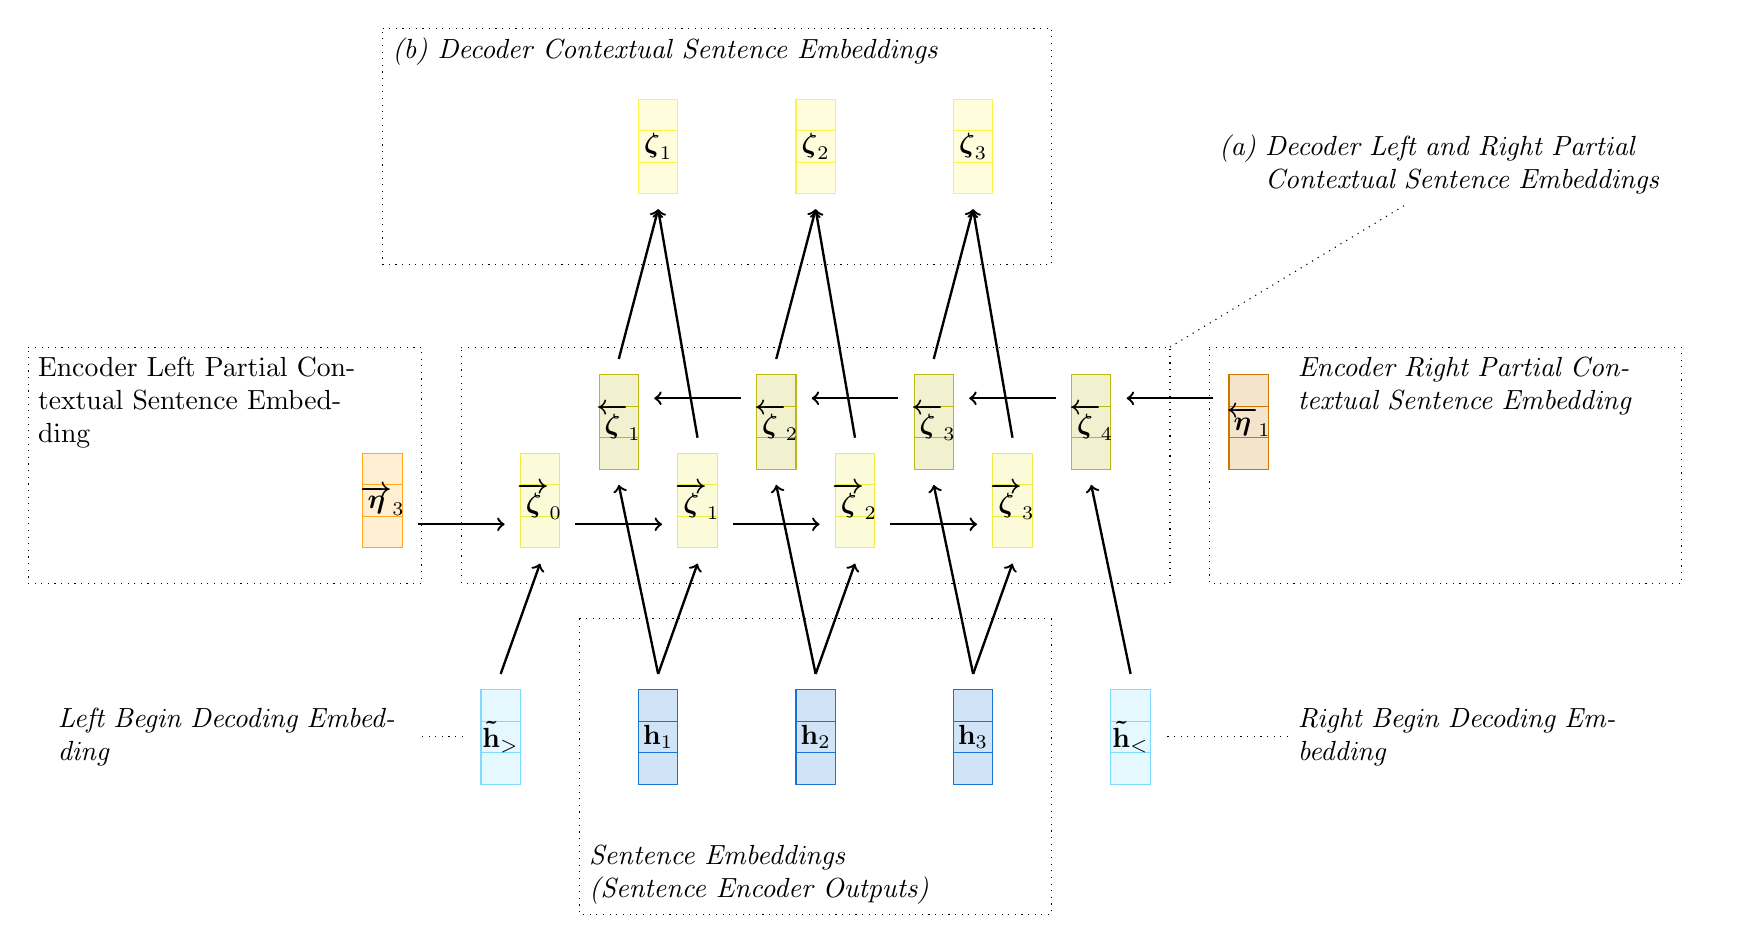
\begin{tikzpicture}[
  dep/.style ={
    ->,line width=0.3mm
  },
  hid/.style 2 args={
    rectangle split,
    draw=#2,
    rectangle split parts=#1,
    fill=#2!20,
    minimum width=5mm,
    minimum height=5mm,
    outer sep=2mm},
  mlp/.style 2 args={
    rectangle split,
    rectangle split horizontal,
    draw=#2,
    rectangle split parts=#1,
    fill=#2!20,
    outer sep=2mm},
  sal/.style={
    circle, 
    minimum width=8mm,
    outer sep=2mm,
    draw=#1, 
    fill=#1!20},
]

  \def\stepsize{2}%
  \def\lvlbase{0}%
  \def\lvlheight{3}%
 

    \node[hid={3}{decsentemb}] (s0) at (\stepsize*0, \lvlbase) {};    
    \node at (\stepsize*0, \lvlbase) {$\stsextSent_>$};    


    \node[hid={3}{decsentemb}] (s4) at (\stepsize*4, \lvlbase) {};    
    \node at (\stepsize*4, \lvlbase) {$\stsextSent_{<}$};    

    % Sentence Embeddings    
  \foreach \step in {1,...,3} {
    \node[hid={3}{sentemb}] (s\step) at (\stepsize*\step, \lvlbase) {};    
    \node at (\stepsize*\step, \lvlbase) {$\sentEmb_\step$};    
   }
%    \foreach \step [count=\i from 1] in {5,...,7} {
%        \node[hid={3}{green}] (s\step) at (\stepsize*\step, \lvlbase) {};    
%        \node at (\stepsize*\step, \lvlbase) {$\sentEmb_\i$};    
%    %\draw[->] (i\step.north) -> (e\step.south);
%    }

%       \node[hid={3}{red}] (s4) at (\stepsize*4, \lvlbase) {};    
%       \node at (\stepsize*4, \lvlbase) {$\sentEmb_0$};    
%
%    % RNN hidden states

        \node[hid={3}{rdecemb}] (rrnn_0) 
            at (\stepsize *0+0.5, \lvlbase + \lvlheight) {};    
        \node at (\stepsize *0+0.5, \lvlbase + \lvlheight) 
            {$\stsextRDecHid_0$}; 

        \node[hid={3}{ldecemb}] (lrnn_4) 
            at (\stepsize *4-0.5, \lvlbase + \lvlheight+1.0) {};    
        \node at (\stepsize *4-0.5, \lvlbase + \lvlheight+1.0) 
            {$\stsextLDecHid_4$}; 

        \node[hid={3}{rencemb}] (rrnn_m1) 
            at (-\stepsize +0.5, \lvlbase + \lvlheight) {};    
        \node at (-\stepsize +0.5, \lvlbase + \lvlheight) 
            {$\stsextREncHid_3$}; 

        \node[hid={3}{lencemb}] (lrnn_m1) 
            at (\stepsize*5 -0.5, \lvlbase + \lvlheight+1.0) {};    
        \node at (\stepsize*5 -0.5, \lvlbase + \lvlheight+1.0) 
            {$\stsextLEncHid_1$}; 

            \node[align=left,anchor=north west,text width=4.3cm] (lbl)  
                at (\stepsize*5.0, \lvlbase + \lvlheight*1.65) 
                {\textit{Encoder Right Partial Contextual Sentence Embedding}};    
    %\draw[dotted] (lbl.east) to (s0);
        \draw[rectangle,draw=black,dotted] 
        (\stepsize*4.5,\lvlbase + 1.65*\lvlheight) -- 
        (\stepsize*7.5, \lvlbase + 1.65*\lvlheight) -- 
        (\stepsize*7.5, \lvlbase + 0.65*\lvlheight) --
        (\stepsize*4.5, \lvlbase + 0.65*\lvlheight) --
        (\stepsize*4.5, \lvlbase + 1.65*\lvlheight) ;


        \draw[rectangle,draw=black,dotted] 
        (\stepsize*-3.0,\lvlbase + 1.65*\lvlheight) -- 
        (\stepsize*-0.5, \lvlbase + 1.65*\lvlheight) -- 
        (\stepsize*-0.5, \lvlbase + 0.65*\lvlheight) --
        (\stepsize*-3.0, \lvlbase + 0.65*\lvlheight) --
        (\stepsize*-3.0, \lvlbase + 1.65*\lvlheight) ;

            \node[align=left,anchor=north west,text width=4.3cm] (lbl)  
                at (\stepsize*-3.0, \lvlbase + \lvlheight*1.65) 
                {Encoder Left Partial Contextual Sentence Embedding};    





    \foreach \step in {1,...,3} {
        \node[hid={3}{rdecemb}] (rrnn_\step) 
            at (\stepsize *\step+0.5, \lvlbase + \lvlheight) {};    
        \node at (\stepsize *\step+0.5, \lvlbase + \lvlheight) 
            {$\stsextRDecHid_\step$}; 

        \node[hid={3}{ldecemb}] (lrnn_\step) 
            at (\stepsize *\step-0.5, \lvlbase + \lvlheight+1.0) {};    
        \node at (\stepsize *\step-0.5, \lvlbase + \lvlheight+1.0) 
            {$\stsextLDecHid_\step$}; 


        \node[hid={3}{decctxemb}] (enc_ctx_\step) 
            at (\stepsize *\step, \lvlbase + 2.5*\lvlheight) {};    
        \node at (\stepsize *\step, \lvlbase + 2.5*\lvlheight) 
            {$\stsextDecHid_\step$}; 

        \draw[dep] (s\step.north) -- (lrnn_\step.south);
        \draw[dep] (s\step.north) -- (rrnn_\step.south);

        \draw[dep] (lrnn_\step.north) -- (enc_ctx_\step.south);
        \draw[dep] (rrnn_\step.north) -- (enc_ctx_\step.south);
    }
    \foreach \start [count=\stop from 2] in {1,...,2} {
        \draw[dep] ($ (rrnn_\start.east) - (0,0.3)$) 
            -- ($ (rrnn_\stop.west) - (0,0.3) $);
        \draw[dep] ($(lrnn_\stop.west) + (0,0.3)$) 
            -- ($ (lrnn_\start.east) + (0,0.3)   $);
    }

        \draw[dep] ($ (rrnn_m1.east) - (0,0.3)$) 
            -- ($ (rrnn_0.west) - (0,0.3) $);
        \draw[dep] ($ (rrnn_0.east) - (0,0.3)$) 
            -- ($ (rrnn_1.west) - (0,0.3) $);

            \draw[dep] (s0.north) to (rrnn_0.south);
            \draw[dep] (s4.north) to (lrnn_4.south);

        \draw[dep] ($ (lrnn_m1.west) + (0,0.3)$) 
            -- ($ (lrnn_4.east) + (0,0.3) $);

        \draw[dep] ($ (lrnn_4.west) + (0,0.3)$) 
            -- ($ (lrnn_3.east) + (0,0.3) $);

%    \foreach \step [count=\i from 0] in {4,...,7} {
%        \node[hid={3}{orange}] (rnn_\step) 
%            at (\stepsize *\step, \lvlbase + \lvlheight) {};    
%        \node at (\stepsize *\step, \lvlbase + \lvlheight) {$\xDecHid_\i$}; 
%    }
%
%    \foreach \step in {1,...,6} {
%        \draw[dep] (s\step.north) to (rnn_\step.south);
%    }
%    \foreach \start [count=\stop from 2] in {1,...,5} {
%        \draw[dep] (rnn_\start.east) to (rnn_\stop.west);
%    }
%
%
%%    \foreach \step [count=\i from 1] in {4,...,6} {
%%        \node[hid={3}{green}] (ctx_\i) 
%%            at (\stepsize *\step, \lvlbase + 2*\lvlheight) {};    
%%        \node at (\stepsize *\step, \lvlbase + 2*\lvlheight) {$\xPredHid_\i$}; 
%%        \draw[dep] (rnn_\step.north) to (ctx_\i.south);
%%        \draw[dep] (rnn_\i.north) to (ctx_\i.south west);
%%        \node[sal={blue}] (sal_\i) at (\stepsize * \step,\lvlbase + 3*\lvlheight) {};
%%        \node at (\stepsize * \step,\lvlbase + 3*\lvlheight) {$\bsal_\i$};
%%        \draw[dep] (ctx_\i.north) to (sal_\i.south);
%%    }
%%
%%    \foreach \step [count=\i from 1] in {5,...,6} {
%%        \draw[dep] (sal_\i) -- (\stepsize * \step - \stepsize / 2,
%%                            \lvlbase + 3*\lvlheight) 
%%                     -- (\stepsize * \step - \stepsize / 2,
%%                            \lvlbase + 0* \lvlheight) -> (s\step) ;
%%
%%    }
%%    \draw[dep] (s1.south) -- ($ (s1.south) + (0,-0.3)$) --($ (s5.south) + (0,-0.3)$) -- (s5.south);
%%
%%    \draw[dep] (s2.south) -- ($ (s2.south) + (0,-0.5)$) --($ (s6.south) + (0,-0.5)$) -- (s6.south);
%%
%%    \draw[rectangle,draw=black,dotted] 
%%        (\stepsize * 3.5,\lvlbase + 3.5*\lvlheight) -- 
%%        (\stepsize*6.5, \lvlbase + 3.5*\lvlheight) -- 
%%        (\stepsize*6.5, \lvlbase + 2.6*\lvlheight) --
%%        (\stepsize*3.5, \lvlbase + 2.6*\lvlheight) --
%%        (\stepsize*3.5, \lvlbase + 3.5*\lvlheight) ;
%%
%%    \node[align=left,anchor=north west] 
%%        at (\stepsize * 3.5,\lvlbase + 3.5*\lvlheight) 
%%        {\textit{Salience Estimates}};
%%
%%    \draw[rectangle,draw=black,dotted] 
%%        (\stepsize*0.5,\lvlbase + 2.5*\lvlheight) -- 
%%        (\stepsize*6.5, \lvlbase + 2.5*\lvlheight) -- 
%%        (\stepsize*6.5, \lvlbase + 1.5*\lvlheight) --
%%        (\stepsize*0.5, \lvlbase + 1.5*\lvlheight) --
%%        (\stepsize*0.5, \lvlbase + 2.5*\lvlheight) ;
%%
%%    \node[align=left,anchor=north west] 
%%        at (\stepsize * 0.5,\lvlbase + 2.5*\lvlheight) 
%%        {\textit{Contextual Sentence Embeddings}};
%%
%%    \draw[rectangle,draw=black,dotted] 
%%        (\stepsize*-0.5,\lvlbase + 0.5*\lvlheight) -- 
%%        (\stepsize*3.5, \lvlbase + 0.5*\lvlheight) -- 
%%        (\stepsize*3.5, \lvlbase + -0.9*\lvlheight) --
%%        (\stepsize*-0.5, \lvlbase + -0.9*\lvlheight) --
%%        (\stepsize*-0.5, \lvlbase + 0.5*\lvlheight) ;
%%
%%    \node[align=left,anchor=south west] 
%%        at (\stepsize * -0.5,\lvlbase + -0.9*\lvlheight) 
%%        {\textit{Sentence Embeddings}\\\textit{(Sentence Encoder Output)}};
%%
%%    \draw[rectangle,draw=black,dotted] 
%%        (\stepsize*4.3,\lvlbase + 0.5*\lvlheight) -- 
%%        (\stepsize*6.5, \lvlbase + 0.5*\lvlheight) -- 
%%        (\stepsize*6.5, \lvlbase + -0.9*\lvlheight) --
%%        (\stepsize*4.3, \lvlbase + -0.9*\lvlheight) --
%%        (\stepsize*4.3, \lvlbase + 0.5*\lvlheight) ;
%%
%%    \node[align=left,anchor=south west] 
%%        at (\stepsize * 4.3,\lvlbase + -0.9*\lvlheight) 
%%        {\textit{Salience Gated}\\\textit{Sentence Embeddings}};
%%

    

    \draw[rectangle,draw=black,dotted] 
        (\stepsize*-0.75,\lvlbase + 3.0*\lvlheight) -- 
        (\stepsize*3.5, \lvlbase + 3.0*\lvlheight) -- 
        (\stepsize*3.5, \lvlbase + 2.0*\lvlheight) --
        (\stepsize*-0.75, \lvlbase + 2.0*\lvlheight) --
        (\stepsize*-0.75, \lvlbase + 3.0*\lvlheight) ;

    \node[align=left,anchor=north west] 
        at (-0.75 *\stepsize,\lvlbase + 3.0*\lvlheight) 
        {\textit{(b) Decoder Contextual Sentence Embeddings}};

        \draw[rectangle,draw=black,dotted] 
        (\stepsize*0.5,\lvlbase + 0.5*\lvlheight) -- 
        (\stepsize*3.5, \lvlbase + 0.5*\lvlheight) -- 
        (\stepsize*3.5, \lvlbase - 0.75*\lvlheight) --
        (\stepsize*0.5, \lvlbase - 0.75*\lvlheight) --
        (\stepsize*0.5, \lvlbase + 0.5*\lvlheight) ;

    \node[align=left,anchor=south west] 
        at (0.5 *\stepsize,\lvlbase - 0.75*\lvlheight) 
        {\textit{Sentence Embeddings}\\\textit{(Sentence Encoder Outputs)}};

        \draw[rectangle,draw=black,dotted] 
        (\stepsize*-0.25,\lvlbase + 1.65*\lvlheight) -- 
        (\stepsize*4.25, \lvlbase + 1.65*\lvlheight) -- 
        (\stepsize*4.25, \lvlbase + 0.65*\lvlheight) --
        (\stepsize*-0.25, \lvlbase + 0.65*\lvlheight) --
        (\stepsize*-0.25, \lvlbase + 1.65*\lvlheight) ;

    \node[align=left,anchor=south west,text width=6.4cm] 
    (lbl) at (4.5 *\stepsize,\lvlbase + 2.25*\lvlheight) 
        {\textit{(a) Decoder Left and Right Partial \phantom{(a) }Contextual Sentence Embeddings}};

    \draw[dotted] (\stepsize*4.25, \lvlbase + 1.65*\lvlheight) to (lbl);


    \node[align=left,anchor=west,text width=4.2cm] (lbl)  at (\stepsize*5, \lvlbase) {\textit{Right Begin Decoding Embedding}};    
    \draw[dotted] (lbl.west) to (s4);

    \node[align=left,anchor=east,text width=4.5cm] (lbl)  at (\stepsize-3, \lvlbase) {\textit{Left Begin Decoding Embedding}};    
    \draw[dotted] (lbl.east) to (s0);


\end{tikzpicture}}
\end{minipage}}
\caption{Schematic for the decoder contextual sentence embeddings as computed by the \stsext~sentence extractor.}
\label{fig:stsext2}

\end{figure}




The final output of each encoder \gru~initializes a separate decoder \gru~which
is then run over the sentence embeddings a second time, \\


%\noindent\fcolorbox{rdecemb}{rdecemb!20!}{\textit{(\hyperref[fig:stsext2]{Figure~\ref{fig:stsext2}.a}) Decoder Left and Right Partial Contextual Sentence Embeddings}}\\[-40pt]
\noindent{\textit{(\hyperref[fig:stsext2]{Figure~\ref{fig:stsext2}.a}) Decoder Left and Right Partial Contextual Sentence Embeddings}}\\[-40pt]
\begin{align}
\stsextRDecHid_0 & = \fgru\left(\stsextSent_>,   \stsextREncHid_\docSize; \stsextRDecParams\right),\\ 
        \stsextRDecHid_i & = \fgru(
            \sentEmb_i,  \stsextRDecHid_{i-1}; 
            \stsextRDecParams) &
    \forall i : i \in \{1,\ldots,\docSize\}, \\
\stsextLDecHid_{\docSize+1} & = \fgru\left(\stsextSent_<, \stsextLEncHid_1;\stsextLDecParams\right),\\ 
        \stsextLDecHid_i & = \fgru(
            \sentEmb_i,  \stsextLDecHid_{i+1}; 
            \stsextLDecParams) &
    \forall i : i \in \{1,\ldots,\docSize\}, 
\end{align}
where $\stsextSent_>$ and $\stsextSent_<$ are special ``begin decoding'' input
embeddings for the forward and backward decoder respectively,
$\stsextRDecHid_i, \stsextLDecHid_i \in \reals^{\stsextRNNDim}$, and
$\stsextRDecParams$ and $\stsextLDecParams$ are the parameters for the forward
and backward decoder \gru s respectively.

The decoder left and right partial contextual sentence embeddings
($\stsextRDecHid_i$ and $\stsextLDecHid_i$) are then concatenated to form the
decoder contextual sentence embeddings,\\

%\noindent\fcolorbox{decctxemb}{decctxemb!20!}{\textit{(\hyperref[fig:stsext2]{Figure~\ref{fig:stsext2}.b}) Decoder Contextual Sentence Embeddings}}\\[-20pt]
\noindent{\textit{(\hyperref[fig:stsext2]{Figure~\ref{fig:stsext2}.b}) Decoder Contextual Sentence Embeddings}}\\[-20pt]
\begin{align}
        \stsextDecHid_i & = \left[\begin{array}{c}
            \stsextRDecHid_i\\ 
            \stsextLDecHid_i\end{array}\right] &
    \forall i :  i \in \{1,\ldots,\docSize\}.
\end{align}


\begin{figure}[p]
\fbox{\begin{minipage}{\textwidth}
\center
\scalebox{0.75}{
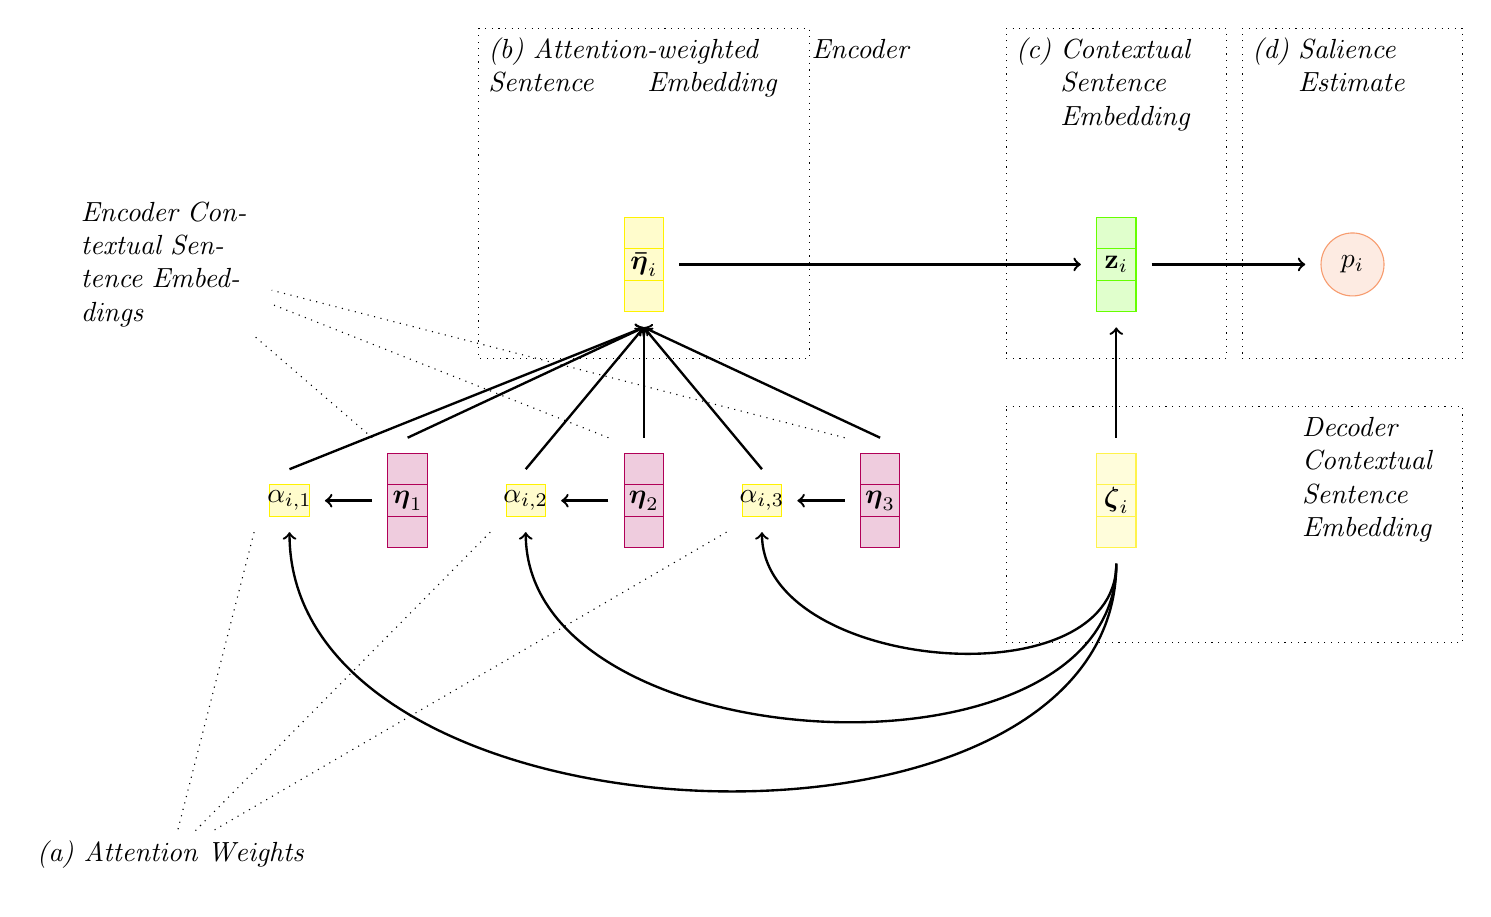
\begin{tikzpicture}[
  dep/.style ={
    ->,line width=0.3mm
  },
  hid/.style 2 args={
    rectangle split,
    draw=#2,
    rectangle split parts=#1,
    fill=#2!20,
    minimum width=5mm,
    minimum height=5mm,
    outer sep=2mm},
  mlp/.style 2 args={
    rectangle split,
    rectangle split horizontal,
    draw=#2,
    rectangle split parts=#1,
    fill=#2!20,
    outer sep=2mm},
  sal/.style={
    circle, 
    minimum width=8mm,
    outer sep=2mm,
    draw=#1, 
    fill=#1!20},
]

  \def\stepsize{3}%
  \def\lvlbase{0}%
  \def\lvlheight{3}%
 


    % Sentence Embeddings    
  \foreach \step in {1,...,3} {
    \node[hid={3}{encctxemb}] (enc\step) at (\stepsize*\step, \lvlbase) {};    
    \node at (\stepsize*\step, \lvlbase) {$\stsextEncHid_\step$};    
   }

  \foreach \step in {1,...,3} {
    \node[hid={1}{yellow}] (a\step) at (\stepsize*\step-0.5*\stepsize, \lvlbase) {};    
    \node at (\stepsize*\step-0.5*\stepsize, \lvlbase) {$\stsextAttn_{i,\step}$};    

    \draw[dep] (enc\step.west) to (a\step.east);
   }


    \node[hid={3}{decctxemb}] (deci) at (\stepsize*4, \lvlbase) {};    
    \node at (\stepsize*4, \lvlbase) {$\stsextDecHid_i$};    


    \draw[dep] (deci.south) to [out=270,in=270] (a3.south);
    \draw[dep] (deci.south) to [out=270,in=270] (a2.south);
    \draw[dep] (deci.south) to [out=270,in=270] (a1.south);

    \node[hid={3}{yellow}] (encattn) at (\stepsize*2, \lvlbase+\lvlheight) {};    
    \node at (\stepsize*2, \lvlbase+\lvlheight) {$\stsextAttnHid_i$};    


    \node[hid={3}{ctxemb}] (ctxi) at (\stepsize*4, \lvlbase+\lvlheight) {};    
    \node at (\stepsize*4, \lvlbase+\lvlheight) {$\stsextHid_i$};    

        \node[sal={sal}] (sal) at (\stepsize * 5,\lvlbase + \lvlheight) {};
        \node at (\stepsize * 5,\lvlbase + \lvlheight) {$\psal_i$};

    \draw[dep] (ctxi) to (sal);
    \draw[dep] (deci.north) to (ctxi.south);
    \draw[dep] (encattn.east) to (ctxi.west);

    \node[text width=2.3cm] (info) at (0,\lvlbase + \lvlheight) {\textit{Encoder Contextual Sentence Embeddings}};
    \draw[dotted] (enc1.north west) to (info);
    \draw[dotted] (enc2.north west) to (info);
    \draw[dotted] (enc3.north west) to (info);
    \node (info) at (0,\lvlbase - 1.5*\lvlheight) {\textit{(a) Attention Weights}};
    \draw[dotted] (a1.south west) to (info);
    \draw[dotted] (a2.south west) to (info);
    \draw[dotted] (a3.south west) to (info);

    \foreach \step in {1,...,3} {
        \draw[dep] (a\step.north) to (encattn.south);
        \draw[dep] (enc\step.north) to (encattn.south);
    }


    \node[align=left,anchor=north west,text width=5.5cm] at (\stepsize*2-2.1,2.0*\lvlheight+\lvlbase)
    {\textit{(b) Attention-weighted \phantom{(b) }Encoder Sentence \phantom{(b) }Embedding}};
\draw[rectangle,draw=black,dotted] 
        (\stepsize*2.0-2.1, \lvlbase + 2.0*\lvlheight) -- 
        (\stepsize*2.0+2.1, \lvlbase + 2.0*\lvlheight) -- 
        (\stepsize*2.0+2.1, \lvlbase + 0.6*\lvlheight) --
        (\stepsize*2.0-2.1, \lvlbase + 0.6*\lvlheight) --
        (\stepsize*2.0-2.1, \lvlbase + 2.0*\lvlheight) ;




    \node[align=left,anchor=north west,text width=2.5cm] at (\stepsize*4-1.4,2.0*\lvlheight+\lvlbase)
    {\textit{(c) Contextual \phantom{(c) }Sentence \phantom{(c) }Embedding}};
\draw[rectangle,draw=black,dotted] 
        (\stepsize*4.0-1.4, \lvlbase + 2.0*\lvlheight) -- 
        (\stepsize*4.0+1.4, \lvlbase + 2.0*\lvlheight) -- 
        (\stepsize*4.0+1.4, \lvlbase + 0.6*\lvlheight) --
        (\stepsize*4.0-1.4, \lvlbase + 0.6*\lvlheight) --
        (\stepsize*4.0-1.4, \lvlbase + 2.0*\lvlheight) ;


    \node[align=left,anchor=north west,text width=2.5cm] at (\stepsize*5-1.4,2.0*\lvlheight+\lvlbase)
{\textit{(d) Salience \phantom{(d) }Estimate}};
\draw[rectangle,draw=black,dotted] 
        (\stepsize*5.0-1.4, \lvlbase + 2.0*\lvlheight) -- 
        (\stepsize*5.0+1.4, \lvlbase + 2.0*\lvlheight) -- 
        (\stepsize*5.0+1.4, \lvlbase + 0.6*\lvlheight) --
        (\stepsize*5.0-1.4, \lvlbase + 0.6*\lvlheight) --
        (\stepsize*5.0-1.4, \lvlbase + 2.0*\lvlheight) ;


    \draw[rectangle,draw=black,dotted] 
        (\stepsize*4.0-1.4, \lvlbase + 0.4*\lvlheight) -- 
        (\stepsize*5.0+1.4, \lvlbase + 0.4*\lvlheight) -- 
        (\stepsize*5.0+1.4, \lvlbase - 0.6*\lvlheight) --
        (\stepsize*4.0-1.4, \lvlbase - 0.6*\lvlheight) --
        (\stepsize*4.0-1.4, \lvlbase + 0.4*\lvlheight) ;


    \node[align=left,anchor=north east,text width=2.5cm] at (\stepsize*5+1.4,0.4*\lvlheight + \lvlbase)
    {\textit{\phantom{(a) }Decoder \phantom{(a) }Contextual \phantom{(a) }Sentence \phantom{(a) }Embedding}};


\end{tikzpicture}}
\caption{Attention layer, contextual sentence embedding, and salience
estimation layer for the \stsext~extractor.}
\label{fig:stsext3}
\end{minipage}}
\end{figure}



\clearpage

Each decoder contextual sentence embedding $\stsextDecHid_i$ then attends to
the encoder contextual sentence embeddings $\stsextEncHid_1,\ldots,
\stsextEncHid_\docSize$, to produce an attention-weighted encoder sentence
embedding $\stsextAttnHid_i$,\\
    
%\noindent\fcolorbox{yellow}{yellow!20!}{\textit{(\hyperref[fig:stsext3]{Figure~\ref{fig:stsext3}.a}) Attention Weights}}\\[-20pt]
\noindent{\textit{(\hyperref[fig:stsext3]{Figure~\ref{fig:stsext3}.a}) Attention Weights}}\\[-20pt]
\begin{align}
    \stsextAttn_{i,j} & = 
        \frac{\exp \left(\stsextDecHid_i \cdot  \stsextEncHid_j \right)}{
            \sum_{j^\prime=1}^{\docSize}\exp\left(  
                \stsextDecHid_i \cdot  \stsextEncHid_{j^\prime} \right)} &
    \forall i : i \in \{1,\ldots,\docSize\}, 
\end{align}
%\noindent\fcolorbox{yellow}{yellow!20!}{\textit{(\hyperref[fig:stsext3]{Figure~\ref{fig:stsext3}.b}) Attention-weighted Encoder Sentence Embeddings}}\\[-20pt]
\noindent{\textit{(\hyperref[fig:stsext3]{Figure~\ref{fig:stsext3}.b}) Attention-weighted Encoder Sentence Embeddings}}\\[-20pt]
\begin{align}
    \stsextAttnHid_i & = 
        \sum_{j=1}^{\docSize} \alpha_{i,j} \left[\begin{array}{c}
            \stsextREncHid_j\\ 
            \stsextLEncHid_j\end{array}\right] & 
    \forall i : i \in \{1,\ldots,\docSize\}.
\end{align}

The attention-weighted encoder sentence embeddings and the decoder contextual
sentence embedding are then concatenated and fed through a \feedforward~layer
to produce the $i^\textrm{th}$ contextual sentence embedding $\stsextHid_i$,
which is itself fed through a final \feedforward~layer to compute the
$i^\textrm{th}$ salience estimate $\nnpsal_i =
\nnmodel(\nnsal_i=1|\sentEmb_1,\ldots,\sentEmb_\docSize;\xParams)$,\\

%\noindent\fcolorbox{ctxemb}{ctxemb!20!}{\textit{(\hyperref[fig:stsext3]{Figure~\ref{fig:stsext3}.c}) Contextual Sentence Embeddings}}\\[-20pt]
\noindent{\textit{(\hyperref[fig:stsext3]{Figure~\ref{fig:stsext3}.c}) Contextual Sentence Embeddings}}\\[-20pt]
\begin{align}
    \stsextHid_i &= \relu\left(\stsextHidWeight \left[\begin{array}{c}
        \stsextAttnHid_i \\ 
        \stsextDecHid_i \end{array}\right] 
        + \stsextHidBias \right) &
    \forall i : i \in \{1,\ldots,\docSize\},
\end{align}


%\noindent\fcolorbox{sal}{sal!20!}{\textit{(\hyperref[fig:stsext3]{Figure~\ref{fig:stsext3}.d}) Salience Estimates}}\\[-40pt]
\noindent{\textit{(\hyperref[fig:stsext3]{Figure~\ref{fig:stsext3}.d}) Salience Estimates}}\\[-40pt]
\begin{align}
\nnpsal_i =    \nnmodel(\nnsal_i=1|\sentEmb_1, \ldots,\sentEmb_\docSize;\xParams)& = 
            \sigma\left(\stsextPredWeight \stsextHid_i + \stsextPredBias  
            \right) &
    \forall i : i \in \{1,\ldots,\docSize\}.
\end{align}
where $\stsextHidWeight \in \reals^{\stsextHidDim \times 3\stsextRNNDim}$,
$\stsextHidBias \in \reals^{\stsextHidDim}$, 
$\stsextPredWeight \in \reals^{1 \times \stsextHidDim}$, and
$\stsextPredBias \in \reals$ are model parameters.
The complete set of \stsext~extractor parameters is 
\[\xParams = \left\{ \stsextREncParams, \stsextLEncParams,
        \stsextRDecParams, \stsextLDecParams, \stsextHidWeight, \stsextHidBias, \stsextPredWeight, \stsextPredBias, \right\}. \]
In our experiments, we set $\stsextRNNDim=300$, $\stsextHidDim=100$.  Dropout
with drop probability of 0.25 is applied to $\stsextREncHid_i,
\stsextLEncHid_i, \stsextRDecHid_i, \stsextLDecHid_i$, and $\stsextHid_i$ for
all $i \in \{1,\ldots,\docSize\}$.

\subsubsection{Comparison of Sentence Extractors}

All of the extractors rely on running at least one \gru~over the sentence
embeddings to propagate contextual information of neighboring sentences to
$\xHid_i$. However, only the \clext~and \srext~extractors rely on
$\psal_1,\ldots,\psal_{i-1}$ to compute $\psal_i$.  After the \gru~layers are
computed in the \rnnext~and \stsext~extracts, all salience estimates can be
computed in parallel; the \clext~and \srext~must make their salience
predictions sequentially.  Additionally, we hypothesize that including this
dependence is not necessary to achieve good performance, as similar
information about the salience of neighboring sentences will already be
captured in the left and right partial contextual sentence embeddings used to
construct $\xHid_i$.

\subsection{Inference and Summary Generation} \label{sec:inference}

Given a setting of encoder and extractor architectures, and the appropriate
embedding, encoder, and extractor parameters ($\embParams$, $\sentEncParams$,
and $\xParams$ respectively), we can compute the probability of a salience
label sequence given a document, $\model\left(\bsals|\doc;\theta\right)$, as 
\begin{align*}
\model\left(\bsals|\doc;\theta\right) &= \model\Big(\bsals|
\sentEnc\big(\embLayer\left(\sent_1;\embParams\right),\ldots,\embLayer\left(\sent_\docSize;\embParams\right)  ;\sentEncParams\big);\xParams\Big) \\
    & = \prod_{i=1}^\docSize \nnpsal_i^{\nnsal_i} (1 - \nnpsal_i)^{(1- \nnsal_i)}.
\end{align*}
Since even in the autoregressive case discrete extraction decisions are never
fed back into the model\footnote{In the autoregressive extractors, the salience
estimates $\nnpsal_i$ are fed back into the model to compute
$\nnpsal_{i+1},\ldots, \nnpsal_\docSize$. However, since these quantities are
not determined by whether or not the model actually extracts sentence
$\sent_i$, they do not create a combinatorial search space.} we can easily find
the most likely extractive sequence 
\[ \nnpredsals = \argmax_{\nnsals\in\labelSpace} \model\left(\nnsals|\doc;\params\right),
\] 
where 
\[\nnpredsal_i = \begin{cases}
       1 & \textrm{if $\nnpsal_i > 0.5$} \\ 0 & \textrm{otherwise}. 
\end{cases}
\]

This method of inference does not take into account the summary word budget
$\wordbudget$ and the resulting $\predbsals$ may imply an extract summary that
is either too short or too long with respect to the budget constraint. Overly
long summaries are less of a problem because they can always be truncated.
Short summaries, however, will suffer more in evaluation as \rouge-recall
monotonically increases with summary size until reaching the word budget.
Additionally, for fair comparisons between systems, summary lengths should
always be the same size \citep{napoles2011}.

To account for this and obtain a summary of length $\wordbudget$, we first
compute $\nnpsal_1,\ldots,\nnpsal_\docSize$. Then we sort the sentences  in
descending order $\sent_{\pi_1}, \ldots, \sent_{\pi_\docSize}$ where
$\psal_{\pi_i} \ge \psal_{\pi_{i+1}}$. We then construct the extract summary by
selecting the first $k$ sentences such that $\sum_{i=1}^{k-1} \sentSize_{\pi_i}
< \wordbudget \le \sum_{i=1}^{k} \sentSize_{\pi_i}$ (i.e., the first $k$
sentences that  meet or exceed the length budget). When evaluating or
displaying summaries, we show the extracted sentences in the original document
order since this improves the coherence, and we truncate the final sentence
where it exceeds $\wordbudget$.

\section{Datasets}
\label{sec:datasets}

We perform our experiments across six corpora from varying domains to
understand how different biases within each domain can affect content
selection. The corpora come from the news domain (CNN-DailyMail, New York
Times, DUC), personal narratives domain (Reddit), workplace meetings (AMI), and
medical journal articles (PubMed). See \autoref{tab:data} for dataset
statistics.

\paragraph{CNN-DailyMail} We use the preprocessing and training, validation,
and test splits of \citet{see2017}.  This corpus is a mix of news on different
topics including politics, sports, and entertainment.

\paragraph{New York Times}The New York Times (NYT) corpus
\citep{sandhaus2008new} contains two types of abstracts for a subset of its
articles. The first summary is an archival abstract and the second is a shorter
online teaser meant to entice a viewer of the webpage to click to read more.
From this collection, we take all articles that have a concatenated summary
length of at least 100 words.  We create training, validation, and test splits
by partitioning on dates; we use the year 2005 as the validation data, with
training and test partitions including documents before and after 2005
respectively.

\paragraph{DUC} We use the single document summarization data from the 2001 and
2002 Document Understanding Conferences (DUC) \citep{over2002introduction}. We
split the 2001 data into training and validation splits and reserve the 2002
data for testing.

\begin{table}
    \center
    \begin{tabular}{ r  r r r r }
      \toprule
      \textbf{Dataset} & \textbf{Train} & \textbf{Valid} & \textbf{Test} &
        \textbf{Refs} \\
      \midrule
      CNN/DM & 287,113 & 13,368 & 11,490 & 1\\
      NYT & 44,382 & 5,523 & 6,495 & 1.93\\
      DUC & 516 & 91 & 657 & 2 \\
      Reddit & 404 & 24 & 48 & 2 \\
      AMI & 98 & 19 & 20 & 1 \\
      PubMed & 21,250 & 1,250 & 2,500 & 1\\
      \bottomrule
    \end{tabular}
   \caption{Sizes of the training, validation, test splits for each dataset
   and the average number of test set human reference summaries per document.}
   \label{tab:data}
\end{table}




\paragraph{AMI} The AMI corpus \citep{carletta2005ami} is a collection of real
and staged office meetings annotated with text transcriptions, along with
abstractive summaries. We use the official train, validation, and test splits
as proposed by the dataset authors.

\paragraph{Reddit} \citet{ouyang2017crowd} collected a corpus of personal
stories shared on Reddit\footnote{\url{www.reddit.com}} along with multiple
extractive and abstractive summaries. We randomly split this data using roughly
three and five percent of the data for validation and testing respectively.

\paragraph{PubMed}{We created a corpus of 25,000 randomly sampled medical
journal articles from the PubMed Open Access
Subset.\footnote{\url{https://www.ncbi.nlm.nih.gov/pmc/tools/openftlist/}} We
only included articles if they were at least 1,000 words long and had an
abstract of at least 50 words in length.  We used the article abstracts as the
ground truth human summaries.}

\subsection{Ground Truth Extract Summaries} \label{sec:labelgen} Since the
datasets above typically only have reference abstract summaries, we do not
explicitly have document/salience judgement pairs $(\doc, \nnsals)$ with which
to train a model. In order to obtain $\nnsals$, we first construct a ``ground
truth'' reference extract summary $\extractSummary \subseteq \doc$ by greedily
selecting sentences $\sent_i \in \doc$ that maximize the \rouge~score
\citep{lin2004} with respect to the reference abstract summaries.  We then
construct the label vector, $\bsals = \left[\bsal_1,\ldots,\bsal_\docSize
\right]$, by assigning positive salience judgements to those sentences in the
extract summary, 
\[
    \bsal_i = \begin{cases} 
        1  & \textrm{if $\sent_i \in \extractSummary$} \\ 
        0 & \textrm{otherwise.} \end{cases} 
\]

\begin{algorithm}[t]
    \DontPrintSemicolon
    \KwData{Input document $\doc = \sent_1, \ldots, \sent_\docSize$, 
          reference abstracts $R$, summary word budget $\wordbudget$.}
   $\bsal_i \gets 0 \quad \forall i \in 1, \ldots, \docSize$ 
   \tcp*{Initialize salience judgements to be $0$.}
   $\extractSummary \gets [\;]$ 
   \tcp*{Initialize summary as empty list.}

   \While(\tcp*[f]{While summary word count $\le$ word budget.}){$\sum_{i=1}^\docSize \bsal_i \sentSize_i \le \wordbudget $}{
%\tcc*[l]{Add the next best sentence to the summary if it will improve the ROUGE score otherwise no improvement can be made so break.}
%
%  ~ \\
    $\hat{i} \gets {\argmax}_{\substack{ i \in \{1, \ldots, n\}, \\ y_i \ne 1 }} 
        \textsc{Rouge}(\extractSummary + [\sent_i], R)$
    \tcp*{Find next best extract.}

%        
%  ~ \\
\eIf{$\textsc{Rouge}(\extractSummary + [ \sent_{\hat{i}} ], R ) > \textsc{Rouge}(\extractSummary, R)$}{
            $\extractSummary \gets \extractSummary + [ \sent_{\hat{i}} ]$
        \tcp*{Update extract and salience judgements.}
        $\bsal_{\hat{i}} \gets 1$ 
        }{ \textbf{break} \tcp*{No further improvements possible, so end.}}
%        
%    
    }
%    
    \KwResult{Salience judgements $\bsals = \left[ \bsal_1, \ldots, \bsal_\docSize\right]$}
    \caption{\textsc{OracleExtractSummaryLabels}}
\label{alg:oraclesum}
\end{algorithm}





The algorithm for constructing the extract summary and salience judgements from
a document and reference abstractive summaries is presented in
\autoref{alg:oraclesum}. It begins by initializing all salience judgements to
zero, $\nnsals = \zeroEmb$, and the extract summary $\extractSummary$ to an
empty list (\hyperref[alg:oraclesum]{Alg.~\ref{alg:oraclesum} lines 1-2}). It
then repeatedly selects the next sentence $\sent_{\hat{i}}$ from the remaining
sentences $\sent_j \notin \extractSummary$ such that adding $\sent_{\hat{i}}$
to $\extractSummary$ maximally improves the marginal \rouge~score
(\hyperref[alg:oraclesum]{Alg.~\ref{alg:oraclesum} lines 3-9}).  If adding
$\sent_{\hat{i}}$ yields improvement, $\extractSummary$ is updated, and
$\nnsal_{\hat{i}}$ is set to $1$
(\hyperref[alg:oraclesum]{Alg.~\ref{alg:oraclesum} lines 6-7}). The algorithm
terminates when the size of extract summary, $\sum_{i=1}^\docSize \nnsal_i
\sentSize_i$, excedes the word budget $\wordbudget$
(\hyperref[alg:oraclesum]{Alg.~\ref{alg:oraclesum} line  3}) or adding an
additional sentence to $\extractSummary$ does not improve the \rouge~score
(\hyperref[alg:oraclesum]{Alg.~\ref{alg:oraclesum} line 5}).  In our
experiments, we choose to specifically optimize for the \rouge-1 recall (i.e.
unigram recall) rather than \rouge-2 recall similarly to other optimization
based approaches to summarization \citep{sipos2012large,durrett2016learning}
which found this to be the easier target to learn.

\section{Experiments} \label{sec:exps}

For our main experiments, we train every possible pairing of sentence encoder
and extractor architecture ($3\times4=12$) on each of dataset $\mathcal{D} =
\left\{\left(\doc^{(1)}, \nnsals^{(1)}\right),\ldots,
\left(\doc^{(\corpusSize)}, \bsals^{(\corpusSize)}\right) \right\}$.  We use
the trained models to produce extract summaries for the test set, and we then
evaluate summary quality with respect to the reference abstract summaries using
\rouge-2 recall.\footnote{\rouge-1 recall and \rouge-LCS trend similarity in
our experiments so we omit them for space.} We use extract summary word budgets
of $\wordbudget=100$ words for news, and $\wordbudget=75$, $\wordbudget=290$,
and $\wordbudget=200$ for Reddit, AMI, and PubMed respectively.  We also
evaluate using \meteor~\citep{banerjee2005meteor}, which measures precision and
recall of reference words while allowing for more matchings on synonymy or
morphology.  We use the default settings for \meteor. We compute \rouge~with
stopwords removed and without stemming, keeping defaults for all other
parameters.

For each model configuration, we train five different versions using different
random seeds and report the mean evaluation measure.  We estimate statistical
significance by first averaging each document level \rouge~or \meteor~score
over the five random initializations.  We then test the difference between the
best system on each dataset and all other systems using the approximate
randomization test with the Bonferroni correction for multiple comparisons
\citep{riezler2005pitfalls}, testing for significance at the $0.05$ level. 

\subsection{Training}

We train all models to minimize the weighted negative log-likelihood
\[\mathcal{L(\params)} = -\sum_{(\doc,\bsals) \in \corpus } \sum_{i=1}^\docSize \omega(\bsal_i) \log \model\left(\bsal_i|\bsal_1,\ldots,\bsal_{i-1},\doc;\params\right) \]
over the training data $\corpus$ using stochastic gradient descent with the
\textsc{Adam} optimizer \citep{kingma2014adam}. Since positive salience labels
(i.e. $\bsal_i = 1$) are much rarer than negative salience labels, we reweight
the negative log likelihood above, setting
\[\omega(0)=1 \quad \textrm{and}\quad \omega(1) = \docSize_0/\docSize_1\] 
where $\docSize_0$ and $\docSize_1$ 
are the number of training sentences labeled $0$ and $1$ respectively.  We
trained for a maximum of 50 epochs and the best model was selected with early
stopping on the validation set according to ROUGE-2. Each epoch constitutes a
full pass through the dataset. The average stopping epoch was: CNN-DailyMail,
16.2; NYT, 21.36; DUC, 37.11; Reddit, 36.59; AMI, 19.58; PubMed, 19.84.  All
experiments were repeated with five random initializations.     Unless
specified, word embeddings were initialized using pretrained GloVe embeddings
\citep{pennington2014glove} and we did not update them during training. Unknown
words were mapped to a zero embedding.

We use a learning rate of $.0001$ and a dropout rate of $0.25$ for all dropout
layers. We also employ gradient clipping ($-5 < \nabla_\theta < 5$).  Weight
matrix parameters are initialized using Xavier initialization with the normal
distribution \citep{glorot2010understanding} and bias terms are set to $0$.
Hyperparameter settings were found using manual exploration and observing
consistent improvements in \rouge~on the validation set.  We use a batch size
of 32 for all datasets except AMI and PubMed, which are often longer and
consume more memory, for which we use sizes two and four respectively.

For \clext~based models, we train for half of the maximum epochs with teacher
forcing, i.e. we set $\psal_i = 1$ if $\bsal_i = 1$ in the gold data and $0$
otherwise when computing the decoder input $\psal_i \sentEmb_i$. We revert to
the predicted model probability during the second half training and during
test-time inference.

\subsection{Baselines}

\paragraph{Lead} As a baseline we include the lead summary, i.e. taking the
first $\wordbudget$ words of the document as summary, where $\wordbudget$ is
the summary word budget for each dataset (see the first paragraph of
\autoref{sec:exps}). While incredibly simple, this method is still a
competitive baseline for single document summarization, especially on newswire.

\paragraph{Oracle} To measure the performance ceiling, we show the
\rouge/\meteor~scores using the extractive summary $\extractSummary$~which was
a bi-product of our algorithm for obtaining salience labels $\bsals$ (see
\autoref{sec:labelgen} for details). Essentially, this summary represents an
approximate ceiling on \rouge~performance, as it has clairvoyant knowledge of
the human reference summaries for each document.

\begin{table*}[p]
    \center
    %\begin{tabular}{ccggccggccggcc}
    \begin{tabular}{cccccccccccccc}
        \toprule
        \multirow{2}{*}{Extractor} &\multirow{2}{*}{Encoder}  & \multicolumn{2}{c}{\textbf{CNN/DM}} & \multicolumn{2}{c}{\textbf{NYT}} & \multicolumn{2}{c}{\textbf{DUC 2002}} \\
         &  & M & R-2 & M & R-2 & M & R-2 \\
        \midrule
%        Random &  -- & 18.2 & 12.7 & 20.7 & 16.0 & 21.7 & 15.8 & \textbf{20.4} & \textbf{12.9} & 12.7 &  2.0 & 16.9 &  9.3\\
%        \hline
        Lead &  -- & 24.1 & 24.4 & 30.0 & 32.3 & 25.1 & 21.5 \\
%        \hline
%        Tail &  -- & 13.7 &  5.4 & 12.5 &  4.1 & 17.8 &  9.1 & \textbf{19.8} & \textbf{10.0} & 11.5 &  2.7 & 17.0 &  9.9\\
        \hline
        \multirow{3}{*}{RNN} & Avg. & \textbf{25.2} & 25.4 & 29.8 & 34.7 & \textbf{26.8} & 22.7 \\
         & RNN & 25.1 & 25.4 & 29.6 & 34.9 & \textbf{26.8} & 22.6 \\
         & CNN & 25.0 & 25.1 & 29.0 & 33.7 & \textbf{26.7} & \textbf{22.7}\\
        \hline
        \multirow{3}{*}{Seq2Seq} & Avg. & \textbf{25.2} & \textbf{25.6} & \textbf{30.5} & \textbf{35.7} & \textbf{27.0} & \textbf{22.8} \\
         & RNN & \textbf{25.1} & 25.3 & 30.2 & \textbf{35.9} & \textbf{26.7} & 22.5 \\
         & CNN & 25.0 & 25.1 & 29.9 & 35.1 & \textbf{26.7} & \textbf{22.7} \\
        \hline
    \multirow{3}{*}{\begin{tabular}{c} Cheng \\ \& \\ Lapata \end{tabular}} & Avg. & 25.0 & 25.3 & 30.4 & \textbf{35.6} & \textbf{27.1} & \textbf{23.1} \\
         & RNN & 25.0 & 25.0 & \textbf{30.3} & \textbf{35.8} & \textbf{27.0} & \textbf{23.0} \\
         & CNN & \textbf{25.2} & 25.1 & 29.9 & 35.0 & \textbf{26.9} & \textbf{23.0} \\
        \hline
    \multirow{3}{*}{\begin{tabular}{c}Summa \\ Runner \end{tabular} } & Avg. & 25.1 & 25.4 & 30.2 & 35.4 & 26.7 & 22.3 \\
         & RNN & 25.1 & 25.2 & 30.0 & 35.5 & 26.5 & 22.1 \\
         & CNN & 24.9 & 25.0 & 29.3 & 34.4 & 26.4 & 22.2 \\
        \hline
        Oracle & -- & 31.1 & 36.2 & 35.3 & 48.9 & 31.3 &  31.8 \\
        \bottomrule
    \end{tabular}

    \caption{News domain \meteor~(M) and \rouge-2 recall (R-2)  results across all 
        extractor/encoder pairs.
           Results that are statistically indistinguishable from the best 
           system are shown in bold face.}
  \label{tab:newsresults}
\end{table*}

\begin{table*}[p]
    \center
    %\begin{tabular}{ccggccggccggcc}
    \begin{tabular}{cccccccccccccc}
        \toprule
        \multirow{2}{*}{Extractor} &\multirow{2}{*}{Encoder}  &  \multicolumn{2}{c}{\textbf{Reddit}} & \multicolumn{2}{c}{\textbf{AMI}} & \multicolumn{2}{c}{\textbf{PubMed}}\\
         &  & M & R-2 & M & R-2 & M & R-2 \\
        \midrule
%        Random &  -- & 18.2 & 12.7 & 20.7 & 16.0 & 21.7 & 15.8 & \textbf{20.4} & \textbf{12.9} & 12.7 &  2.0 & 16.9 &  9.3\\
%        \hline
        Lead &  -- &  \textbf{20.1} & \textbf{10.9} & 12.3 &  2.0 & 15.9 &  9.3\\
%        \hline
%        Tail &  -- & 13.7 &  5.4 & 12.5 &  4.1 & 17.8 &  9.1 & \textbf{19.8} & \textbf{10.0} & 11.5 &  2.7 & 17.0 &  9.9\\
        \hline
        \multirow{3}{*}{RNN} & Avg. &  \textbf{20.4} & \textbf{11.4} & \textbf{17.0} & \textbf{ 5.5} & 19.8 & 17.0\\
         & RNN &  \textbf{20.2} & \textbf{11.4} & 16.2 & \textbf{ 5.2} & 19.7 & 16.6\\
         & CNN & \textbf{20.9} & \textbf{12.8} & 14.4 &  3.2 & 19.9 & 16.8\\
        \hline
        \multirow{3}{*}{Seq2Seq} & Avg. &  \textbf{20.9} & \textbf{13.6} & \textbf{17.0} & \textbf{ 5.5} & \textbf{20.1} & \textbf{17.7}\\
         & RNN &  \textbf{20.5} & \textbf{12.0} & 16.1 & \textbf{ 5.3} & 19.7 & 16.7\\
         & CNN &  \textbf{20.7} & \textbf{13.2} & 14.2 &  2.9 & 19.8 & 16.9\\
        \hline
    \multirow{3}{*}{\begin{tabular}{c} Cheng \&  Lapata \end{tabular}} & Avg. &  \textbf{20.9} & \textbf{13.6} & \textbf{16.7} & \textbf{ 6.1} & \textbf{20.1} & \textbf{17.7}\\
         & RNN &  \textbf{20.3} & \textbf{12.6} & \textbf{16.3} & \textbf{ 5.0} & 19.7 & 16.7\\
         & CNN &  \textbf{20.5} & \textbf{13.4} & 14.3 &  2.8 & 19.9 & 16.9\\
        \hline
    \multirow{3}{*}{\begin{tabular}{c}Summa Runner \end{tabular} } & Avg. & \textbf{21.0} & \textbf{13.4} & \textbf{17.0} & \textbf{ 5.6} & 19.9 & 17.2\\
         & RNN &\textbf{20.9} & \textbf{12.5} & \textbf{16.5} & \textbf{ 5.4} & 19.7 & 16.5\\
         & CNN &  \textbf{20.4} & \textbf{12.3} & 14.5 &  3.2 & 19.8 & 16.8\\
        \hline
        Oracle & -- &  24.3 &  16.2 &17.8 &  8.7  & 24.1 &25.0 \\
        \bottomrule
    \end{tabular}

    \caption{Non-news domain \meteor~(M) and \rouge-2 recall (R-2)  results across all 
        extractor/encoder pairs.
           Results that are statistically indistinguishable from the best 
           system are shown in bold face.}
  \label{tab:otherresults}
\end{table*}


\section{Results}

The results of our main experiment comparing the different extractors/encoders
on news and non-news domains are shown in \autoref{tab:newsresults} and
\autoref{tab:otherresults} respectively.  Overall, we find no major advantage
when using the \convolutionalneuralnetwork~and \recurrentneuralnetwork~sentence
encoders over the averaging encoder. The best performing encoder/extractor pair
either uses the averaging encoder (five out of six datasets) or the differences
are not statistically significant. 

When looking at extractors, the Seq2Seq extractor is either part of the best
performing system (three out of six datasets) or is not statistically
distinguishable from the best extractor. 

Overall, on the news and medical journal domains, the differences are quite
small with the differences between worst and best systems on the CNN/DM dataset
spanning only .56 of a ROUGE point. While there is more performance variability
in the Reddit and AMI data, there is less distinction among systems: no
differences are significant on Reddit and every extractor has at least one
configuration that is indistinguishable from the best system on the AMI corpus.
This is probably due to the small test size of these datasets.


\begin{table*}[t]
\center
\begin{tabular}{cccm{.45cm}cm{.45cm}cm{.65cm}cm{.65cm}cm{.70cm}cm{.4cm}}
    \toprule
    \multirow{1}{*}{\textbf{Ext.}} &\multirow{1}{*}{\textbf{Emb.}}  & \multicolumn{2}{c}{\textbf{CNN/DM}} & \multicolumn{2}{c}{\textbf{NYT}} & \multicolumn{2}{c}{\textbf{DUC}} & \multicolumn{2}{c}{\textbf{Reddit}} & \multicolumn{2}{c}{\textbf{AMI}} & \multicolumn{2}{c}{\textbf{PubMed}}\\
   %  &  & R-2 & R-2 & R-2 & R-2 & R-2 & R-2\\
   % \hline
    \midrule
    \multirow{2}{*}{RNN} & Fixed & \textbf{25.4} & & \textbf{34.7} & & \textbf{22.7} & & \textbf{11.4} & & \textbf{ 5.5} & & \textbf{17.0}\\
                         & F.-T. & 25.2& \scriptsize{(0.2)} & 34.3 &\scriptsize{(0.4)} & \textbf{22.6} & \scriptsize{(0.1)} & \textbf{11.3} & \scriptsize{(0.1)} & \textbf{ 5.3} & \scriptsize{(0.2)} & 16.4& \scriptsize{(0.6)}\\
    \hline
    \multirow{2}{*}{Seq2Seq} & Fixed & \textbf{25.6} && \textbf{35.7}& & \textbf{22.8}& & \textbf{13.6} &&  5.5 && \textbf{17.7}\\
   & F.-T. & 25.3 &\scriptsize{(0.3)} & \textbf{35.7}& \scriptsize{(0.0)} & \textbf{22.9} & \scriptsize{(-0.1)} & \textbf{13.8} &\scriptsize{ (-0.2)} & \textbf{ 5.8} & \scriptsize{(-0.3)} & 16.9 & \scriptsize{(0.8)}\\
    \hline
    \multirow{2}{*}{C\&L} & Fixed & \textbf{25.3} && \textbf{35.6} && \textbf{23.1} && \textbf{13.6} && \textbf{ 6.1} && \textbf{17.7}&\\
                      & F.-T. & 24.9 &\scriptsize{(0.4)} & 35.4 & \scriptsize{(0.2)} & \textbf{23.0} &\scriptsize{ (0.1)} & \textbf{13.4} &\scriptsize{ (0.2)} & \textbf{ 6.2} &\scriptsize{ (-0.1)} & 16.4 &\scriptsize{ (1.3)} \\
    \hline
\multirow{2}{*}{\begin{tabular}{c} Summa \\ Runner \end{tabular}} & Fixed & \textbf{25.4} && \textbf{35.4} && \textbf{22.3} && \textbf{13.4} && \textbf{ 5.6} & &\textbf{17.2}&\\
                                                                  & F.-T. & 25.1 &\scriptsize{(0.3)} & 35.2 &\scriptsize{(0.2)} & \textbf{22.2} & \scriptsize{(0.1)} & 12.6 & \scriptsize{(0.8)} & \textbf{ 5.8} & \scriptsize{(-0.2)} & 16.8&\scriptsize{ (0.4) }\\
    \bottomrule
\end{tabular}

\caption{ROUGE-2 recall across sentence extractors
    when using fixed pretrained embeddings or when embeddings are fine-tuned (F.-T.) during training. In both cases embeddings
    are initialized with pretrained GloVe embeddings. All extractors use the averaging 
sentence encoder. When both fine-tuned and fixed settings are bolded,
there is no signifcant performance difference. Difference in scores shown in parenthesis.}
\label{tab:embeddings}
\end{table*}

%\begin{table*}
%\center
%\begin{tabular}{| c | c || c | c | c | c | c | c | c | c |}
%\hline
%  &   & \multicolumn{2}{|c|}{cnn-dailymail} & \multicolumn{2}{|c|}{nyt} & \multicolumn{2}{|c|}{duc-sds} & \multicolumn{2}{|c|}{reddit} \\
%system & embeddings & R1 & R2  & R1 & R2  & R1 & R2  & R1 & R2  \\
%\hline
%\multirow{2}{*}{RNN} & fixed & 55.3 & 25.4 & 51.4 & 34.7 & 44.1 & 22.6 & 45.2 & 11.4\\ \cline{2-10}
% & learned & 55.1 & 25.2 & 51.1 & 34.3 & 44.1 & 22.6 & 45.3 & 11.3\\
%\hline
%\multirow{2}{*}{Seq2Seq} & fixed & 55.6 & 25.6 & 52.5 & 35.7 & 44.4 & 22.8 & 49.1 & 13.6\\ \cline{2-10}
% & learned & 55.2 & 25.3 & 52.4 & 35.7 & 44.5 & 22.9 & 49.4 & 13.8\\
%\hline
%\multirow{2}{*}{C\&L} & fixed & 55.1 & 25.3 & 52.3 & 35.6 & 44.8 & 23.1 & 48.3 & 13.6\\ \cline{2-10}
% & learned & 54.8 & 25.0 & 52.1 & 35.4 & 44.6 & 23.0 & 48.6 & 13.5\\
%\hline
%\multirow{2}{*}{SummaRunner} & fixed & 55.3 & 25.4 & 52.1 & 35.4 & 44.0 & 22.3 & 48.8 & 13.4\\ \cline{2-10}
% & learned & 55.0 & 25.1 & 52.0 & 35.2 & 43.8 & 22.1 & 47.8 & 12.6\\
%\hline
%\end{tabular}
%\caption{ROUGE 1 and 2 recall results across different sentence extractors
%    when using learned or pretrained embeddings. In both cases embeddings
%    are initialized with pretrained GloVe embeddings. All results are 
%averaged from five random initializations. All extractors use the averaging 
%sentence encoder.}
%\label{tab:embeddings}
%\end{table*}


\subsection{Ablation Experiments}

In addition to our main evaluation above, we also perform several ablation
experiments to further understand how the various summarization models perform
when certain information is witheld from the model. In particular, we evaluate
the effect of fine-tuning word embeddings, part-of-speech (POS) based
ablations, and sentence-order shuffling.

\paragraph{Word Embedding Fine-tuning} Given that learning a sentence encoder
(averaging has no learned parameters) does not yield significant improvement,
it is natural to consider whether fine-tuning word embeddings is also
necessary.  In \autoref{tab:embeddings} we compare the performance of different
extractors using the averaging encoder, when the word embeddings are held fixed
or fine-tuned during training. In both cases, word embeddings are initialized
with GloVe embeddings trained on a combination of Gigaword and Wikipedia.  When
fine-tuning embeddings, words occurring fewer than three times in the training
data are mapped to an unknown token (with learned embedding).
 
In all but one case, fixed embeddings are as good or better than the fine-tuned
embeddings.  This is a somewhat surprising finding on the CNN/DM data since it
is reasonably large, and learning embeddings should give the models more
flexibility to identify important word features.\footnote{The AMI corpus is an
exception here where learning \emph{does} lead to small performance boosts,
however, only in the Seq2Seq extractor is this diference significant; it is
quite possible that this is an artifact of the very small test set size.} This
suggests that we cannot extract much generalizable learning signal from the
content other than what is already present from initialization.  Even on
PubMed, where the language is quite different from the news/Wikipedia articles
the GloVe embeddings were trained on, fine-tuning leads to significantly worse
results.

\begin{table*}[ht]
\center
\begin{tabular}{ccccccc}
    \toprule
    \multirow{1}{*}{\textbf{Ablation}}  & \multicolumn{1}{c}{\textbf{CNN/DM}} & \multicolumn{1}{c}{\textbf{NYT}} & \multicolumn{1}{c}{\textbf{DUC}} & \multicolumn{1}{c}{\textbf{Reddit}} & \multicolumn{1}{c}{\textbf{AMI}} & \multicolumn{1}{c}{\textbf{PubMed}}\\
    \hline
    all words & \textbf{25.4}\textsuperscript{~} ~~~~~~~ & \textbf{34.7}\textsuperscript{~} ~~~~~~~~& 22.7\textsuperscript{~} ~~~~~~~~& \textbf{11.4}\textsuperscript{~} ~~~~~~~~& 5.5\textsuperscript{~} ~~~~~~~~~& \textbf{17.0}\textsuperscript{~} ~~~~~~~ \\
    -nouns & 25.3\textsuperscript{$\dagger$} \footnotesize{(0.1)}& 34.3\textsuperscript{$\dagger$} \footnotesize{(0.4)}& 22.3\textsuperscript{$\dagger$} ~\footnotesize{(0.4)}& 10.3\textsuperscript{$\dagger$} \footnotesize{(1.1)} & 3.8\textsuperscript{$\dagger$} \footnotesize{(1.7)}& 15.7\textsuperscript{$\dagger$} \footnotesize{(1.3)}\\
    -verbs & 25.3\textsuperscript{$\dagger$} \footnotesize{(0.1)}& 34.4\textsuperscript{$\dagger$} \footnotesize{(0.3)} & 22.4\textsuperscript{$\dagger$} ~\footnotesize{(0.3)}& 10.8\textsuperscript{~} ~\footnotesize{(0.6)} & 5.8\textsuperscript{~} \footnotesize{(-0.3)} & 16.6\textsuperscript{$\dagger$} \footnotesize{(0.4)}\\
    -adj/adv & 25.3\textsuperscript{$\dagger$} \footnotesize{(0.1)}& 34.4\textsuperscript{$\dagger$} \footnotesize{(0.3)} & 22.5\textsuperscript{~} ~\footnotesize{(0.2)} & ~~9.5\textsuperscript{$\dagger$} \footnotesize{(1.9)} & 5.4\textsuperscript{~} ~\footnotesize{(0.1)} & 16.8\textsuperscript{$\dagger$} \footnotesize{(0.2)}\\
    -function & 25.2\textsuperscript{$\dagger$} \footnotesize{(0.2)} & 34.5\textsuperscript{$\dagger$} \footnotesize{(0.2)} & \textbf{22.9}\textsuperscript{$\dagger$} \footnotesize{(-0.2)} & 10.3\textsuperscript{$\dagger$} \footnotesize{(1.1)}& \textbf{6.3}\textsuperscript{$\dagger$} \footnotesize{(-0.8)}& 16.6\textsuperscript{$\dagger$} \footnotesize{(0.4)}\\
    \bottomrule
\end{tabular}

\caption{ROUGE-2 recall after removing nouns, verbs, adjectives/adverbs, and 
    function words. Ablations are
    performed using the averaging sentence encoder and the RNN
extractor. 
Bold indicates best performing system. $\dagger$ indicates significant 
difference with the non-ablated system. Difference in score from \textit{all words} shown in parenthesis.}
\label{tab:ablations}
\end{table*}


\paragraph{POS Ablation} It is also not well explored what word features are
being used by the encoders.  To understand which classes of words were most
important we ran an ablation study, selectively removing nouns, verbs
(including participles and auxiliaries), adjectives \& adverbs, and function
words (adpositions, determiners, conjunctions).  All datasets were
automatically tagged using the spaCy POS
tagger\footnote{https://github.com/explosion/spaCy}.   The embeddings of
removed words were replaced with a zero vector, preserving the order and
position of the non-ablated words in the sentence.  Ablations were performed on
training, validation, and test partitions, using the RNN extractor with
averaging encoder.  Note that while the input to the models has redacted word
classes, the produced summaries are evaluated with all words present. See
\autoref{fig:wordabl} for example inputs under the different word class
ablations.

\begin{figure}
\fbox{\begin{minipage}{\textwidth}
~\\
\begin{minipage}[t]{0.45\textwidth}
\begin{center}\textbf{Nouns Redacted}\end{center}~\\[-50pt]
\begin{singlespace}
\small
\begin{enumerate}
\item \colorbox{black}{hurricane} \colorbox{black}{gilbert} swept toward the \colorbox{black}{dominican} \colorbox{black}{republic} \colorbox{black}{sunday}, and the \colorbox{black}{civil} \colorbox{black}{defense} alerted its heavily populated south \colorbox{black}{coast} to prepare for high \colorbox{black}{winds}, heavy \colorbox{black}{rains} and high \colorbox{black}{seas}.
\item the \colorbox{black}{storm} was approaching from the \colorbox{black}{southeast} with sustained \colorbox{black}{winds} of 75 \colorbox{black}{mph} gusting to 92 \colorbox{black}{mph} .
\item ``There is no \colorbox{black}{need} for \colorbox{black}{alarm},'' civil \colorbox{black}{defense} \colorbox{black}{director} \colorbox{black}{eugenio} \colorbox{black}{cabral} said in a \colorbox{black}{television} \colorbox{black}{alert} shortly before \colorbox{black}{midnight} \colorbox{black}{saturday}.
\item \colorbox{black}{cabral} said \colorbox{black}{residents} of the \colorbox{black}{province} of \colorbox{black}{barahona} should closely follow \colorbox{black}{gilbert}'s \colorbox{black}{movement}.
\end{enumerate}
\end{singlespace}
\end{minipage}~~~~~~~\begin{minipage}[t]{0.45\textwidth}
\begin{center}\textbf{Verbs Redacted}\end{center}~\\[-50pt]
\begin{singlespace}
\small
\begin{enumerate}
\item Hurricane Gilbert \colorbox{black}{swept} toward the Dominican Republic Sunday, and the Civil Defense \colorbox{black}{alerted} its heavily populated south coast \colorbox{black}{to} \colorbox{black}{prepare} for high winds, heavy rains and high seas.
\item The storm \colorbox{black}{was} \colorbox{black}{approaching} from the southeast with sustained winds of 75 mph \colorbox{black}{gusting} to 92 mph.
\item ``There \colorbox{black}{is} no need for alarm,'' Civil Defense Director Eugenio Cabral \colorbox{black}{said} in a television alert shortly before midnight Saturday.
\item Cabral \colorbox{black}{said} residents of the province of Barahona \colorbox{black}{should} closely \colorbox{black}{follow} Gilbert \colorbox{black}{'s} movement.
\end{enumerate}
\end{singlespace}
\end{minipage}

~\\
~\\

\begin{minipage}{0.45\textwidth}
\begin{center}\textbf{Adjectives/Adverbs Redacted}\end{center}~\\[-50pt]
\begin{singlespace}
\small
\begin{enumerate}
\item Hurricane Gilbert swept toward the Dominican Republic Sunday, and the Civil Defense alerted \colorbox{black}{its} \colorbox{black}{heavily} \colorbox{black}{populated} \colorbox{black}{south} coast to prepare for \colorbox{black}{high} winds, \colorbox{black}{heavy} rains and \colorbox{black}{high} seas.
\item The storm was approaching from the southeast with \colorbox{black}{sustained} winds of 75 mph gusting to 92 mph.
\item ``\colorbox{black}{there} is no need for alarm,'' \colorbox{black}{civil} Defense Director Eugenio Cabral said in a television alert \colorbox{black}{shortly} before midnight Saturday.
\item Cabral said residents of the province of Barahona should \colorbox{black}{closely} follow Gilbert's movement.
\end{enumerate}
\end{singlespace}
\end{minipage}~~~~~~~\begin{minipage}{0.45\textwidth}
\begin{center}\textbf{Function Words Redacted}\end{center}~\\[-50pt]
\begin{singlespace}
\small
\begin{enumerate}
\item Hurricane Gilbert swept \colorbox{black}{toward} \colorbox{black}{the} Dominican Republic Sunday, \colorbox{black}{and} \colorbox{black}{the} Civil Defense alerted its heavily populated south coast to prepare \colorbox{black}{for} high winds, heavy rains \colorbox{black}{and} high seas.
\item \colorbox{black}{the} storm was approaching \colorbox{black}{from} \colorbox{black}{the} southeast \colorbox{black}{with} sustained winds \colorbox{black}{of} 75 mph gusting \colorbox{black}{to} 92 mph .
\item ``There is \colorbox{black}{no} need \colorbox{black}{for} alarm,'' Civil Defense Director Eugenio Cabral said \colorbox{black}{in} \colorbox{black}{a} television alert shortly \colorbox{black}{before} midnight Saturday.
\item Cabral said residents \colorbox{black}{of} \colorbox{black}{the} province \colorbox{black}{of} Barahona should closely follow Gilbert's movement.
\end{enumerate}
\end{singlespace}
\end{minipage}

~\\
\end{minipage}}
\caption{The first four sentences from a DUC 2002 article (id: d061j-AP880911-0016) under the different word class ablations. }
\label{fig:wordabl}
\end{figure}


\autoref{tab:ablations} shows the results of the POS tag ablation experiments.
While removing any word class from the representation generally hurts
performance (with statistical significance), on the news domains, the absolute
values of the differences are quite small (.18 on CNN/DM, .41 on NYT, .3 on
DUC) suggesting that the model's predictions are not overly dependent on any
particular word types. 

Qualitatively, we see little difference in outputs produced under the redacted
models.  For example, see \autoref{fig:sumwordabl} where we show output
summaries from the different word class redacted models. All four variants
identify the lead two sentences as most important, while also including
sentences five and six. Three of the summaries also selected sentence 13.  The
summarizers appear to have selected most content from the front of the article
suggesting the lead is identfiable even when different content is ablated.

\begin{figure}[p]
    \fbox{   \begin{minipage}{\textwidth}
 \begingroup
  \setlength{\fboxsep}{0pt}%  
\small 
\textbf{Nouns Redacted}\\
\colorbox{Orchid!25!}{\begin{minipage}{\textwidth}(1) Hurricane Gilbert swept toward the Dominican Republic Sunday, and the Civil Defense alerted its heavily populated south coast to prepare for high winds, heavy rains and high seas.\end{minipage}}\\
\colorbox{Dandelion!25!}{\begin{minipage}{\textwidth}(2) The storm was approaching from the southeast with sustained winds of 75 mph gusting to 92 mph.\end{minipage}}\\
\colorbox{GreenYellow!35!}{\begin{minipage}{\textwidth}(5) An estimated 100,000 people live in the province, including 70,000 in the city of Barahona, about 125 miles west of Santo Domingo.\end{minipage}}\\
\colorbox{ProcessBlue!15!}{\begin{minipage}{\textwidth}(6) Tropical Storm Gilbert formed in the eastern Caribbean and strengthened into a hurricane Saturday night.\end{minipage}}\\
%\colorbox{red!25!}{
\begin{minipage}{\textwidth}(7) The National Hurricane Center in Miami reported its position at 2 a.m. Sunday at latitude 16.1 north, longitude 67.5 west, about 140 miles south of Ponce, Puerto Rico, and 200 miles southeast of Santo Domingo.\end{minipage}\\

\textbf{Verbs Redacted}\\
\colorbox{Orchid!25!}{\begin{minipage}{\textwidth}(1) Hurricane Gilbert swept toward the Dominican Republic Sunday, and the Civil Defense alerted its heavily populated south coast to prepare for high winds, heavy rains and high seas.\end{minipage}}\\
\colorbox{Dandelion!25!}{\begin{minipage}{\textwidth}(2) The storm was approaching from the southeast with sustained winds of 75 mph gusting to 92 mph.\end{minipage}}\\
\colorbox{green!25!}{\begin{minipage}{\textwidth}(13) On Saturday, Hurricane Florence was downgraded to a tropical storm and its remnants pushed inland from the U.S. Gulf Coast.\end{minipage}}\\
\colorbox{ProcessBlue!15!}{\begin{minipage}{\textwidth}(6) Tropical Storm Gilbert formed in the eastern Caribbean and strengthened into a hurricane Saturday night.\end{minipage}}\\
(12) San Juan, on the north coast, had heavy rains and gusts Saturday, but they subsided during the night.\\
\colorbox{GreenYellow!35!}{\begin{minipage}{\textwidth}(5) An estimated 100,000 people live in the province, including 70,000 in the city of Barahona, about 125 miles west of Santo Domingo.\end{minipage}}\\

\textbf{Adjectives/Adverbs Redacted}\\
\colorbox{Dandelion!25!}{\begin{minipage}{\textwidth}(2) The storm was approaching from the southeast with sustained winds of 75 mph gusting to 92 mph.\end{minipage}}\\
\colorbox{Orchid!25!}{\begin{minipage}{\textwidth}(1) Hurricane Gilbert swept toward the Dominican Republic Sunday, and the Civil Defense alerted its heavily populated south coast to prepare for high winds, heavy rains and high seas.\end{minipage}}\\
\colorbox{GreenYellow!35!}{\begin{minipage}{\textwidth}(5) An estimated 100,000 people live in the province, including 70,000 in the city of Barahona, about 125 miles west of Santo Domingo.\end{minipage}}\\
\colorbox{green!25!}{\begin{minipage}{\textwidth}(13) On Saturday, Hurricane Florence was downgraded to a tropical storm and its remnants pushed inland from the U.S. Gulf Coast.\end{minipage}}\\
\colorbox{ProcessBlue!15!}{\begin{minipage}{\textwidth}(6) Tropical Storm Gilbert formed in the eastern Caribbean and strengthened into a hurricane Saturday night.\end{minipage}}\\
(14) Residents returned home, happy to find little damage from 80 mph winds and sheets of rain.\\

\textbf{Function Words Redacted}\\
\colorbox{Orchid!25!}{\begin{minipage}{\textwidth}(1) Hurricane Gilbert swept toward the Dominican Republic Sunday, and the Civil Defense alerted its heavily populated south coast to prepare for high winds, heavy rains and high seas.\end{minipage}}\\
\colorbox{Dandelion!25!}{\begin{minipage}{\textwidth}(2) The storm was approaching from the southeast with sustained winds of 75 mph gusting to 92 mph.\end{minipage}}\\
\colorbox{green!25!}{\begin{minipage}{\textwidth}(13) On Saturday, Hurricane Florence was downgraded to a tropical storm and its remnants pushed inland from the U.S. Gulf Coast.\end{minipage}}\\
\colorbox{ProcessBlue!15!}{\begin{minipage}{\textwidth}(6) Tropical Storm Gilbert formed in the eastern Caribbean and strengthened into a hurricane Saturday night.\end{minipage}}\\
(10) Strong winds associated with the Gilbert brought coastal flooding, strong southeast winds and up to 12 feet feet to Puerto Rico's south coast.\\
\colorbox{GreenYellow!35!}{\begin{minipage}{\textwidth}(5) An estimated 100,000 people live in the province, including 70,000 in the city of Barahona, about 125 miles west of Santo Domingo.\end{minipage}}\\
\endgroup
\end{minipage}}
\caption{Outputs from the word class ablated models when given the document as  input from
\autoref{fig:wordabl}. Original document positions of the extracted sentences are  shown in parenthesis; sentences that are selected by multiple systems
are highlighted in color.}
\label{fig:sumwordabl}
\end{figure}


On the non-news datasets, the ablations have a larger effect (max differences
are 1.89 on Reddit, 2.56 on AMI, and 1.3 on PubMed).  Removing nouns leads to
the largest drop on AMI and PubMed.  Removing adjectives and adverbs leads to
the largest drop on Reddit, suggesting the intensifiers and descriptive words
are useful for identifying important content in personal narratives.
Curiously, removing the function word POS class yields a significant
improvement on DUC 2002 and AMI.

\begin{table*}[t]
\center

\begin{tabular}{cccm{.5cm}cm{.5cm}cm{.5cm}cm{.75cm}cm{.75cm}cm{.5cm}}
    \toprule
    \textbf{Ext.} &\textbf{Order}  & \multicolumn{2}{c}{\textbf{CNN/DM}} & \multicolumn{2}{c}{\textbf{NYT}} & \multicolumn{2}{c}{\textbf{DUC}} & \multicolumn{2}{c}{\textbf{Reddit}} & \multicolumn{2}{c}{\textbf{AMI}} & \multicolumn{2}{c}{\textbf{PubMed}}\\
    \midrule
    \multirow{2}{*}{Seq2Seq} & In-Order & \textbf{25.6} & & \textbf{35.7} && \textbf{22.8}& & \textbf{13.6} && 5.5 && \textbf{17.7} &\\
                             & Shuffled & 21.7&\scriptsize{(3.9)} & 25.6 & \scriptsize{(10.1)} & 21.2 & \scriptsize{(1.6)} &\textbf{13.5} &\scriptsize{(0.1)} &\textbf{6.0} & \scriptsize{(-0.5)}&14.9 &\scriptsize{(2.8)}\\
    \bottomrule
\end{tabular}

\caption{ROUGE-2 recall using models trained on in-order and shuffled
documents. Extractor uses the averaging sentence encoder. 
When both in-order and shuffled settings are bolded,
there is no signifcant performance difference. Difference in scores shown in parenthesis.
}
\label{tab:shuffle}
\end{table*}


\textbf{Sentence Order Shuffling} Sentence position is a well known and
powerful feature for news summarization \citep{hong2014improving}, owing to the
intentional lead bias in the news article
writing\footnote{\url{https://en.wikipedia.org/wiki/Inverted_pyramid_(journalism)}};
it also explains the difficulty in beating the lead baseline for
single-document summarization \citep{nenkova2005b,brandow1995}.  In examining
the generated summaries, we found most of the selected sentences in the news
domain came from the lead paragraph of the document. This is despite the fact
that there is a long tail of sentence extractions from later in the document in
the ground truth extract summaries (31\%, 28.3\%, and 11.4\% of DUC, CNN/DM,
and NYT training extract labels come from the second half of the document).
Because this lead bias is so strong, it is questionable whether the models are
learning to identify important content or just find the start of the document.
We conduct a sentence order experiment where each document's sentences are
randomly shuffled during training. We then evaluate each model performance on
the unshuffled test data, comparing to the model trained on unshuffled data; if
the models trained on shuffled data drop in performance, then this indicates
the lead bias is the relevant factor.

\autoref{tab:shuffle} shows the results of the shuffling experiments.  The news
domains and PubMed suffer a significant drop in performance when the document
order is shuffled. By comparison, there is no significant difference between
the shuffled and in-order models on the Reddit domain, and shuffling actually
improves performance on AMI.  This suggest that position is being learned by
the models in the news/journal article domain even when the model has no
explicit position features, and that this feature is more important than either
content or function words.

\begin{table*}[t]
    \footnotesize
\centering
  \begin{tabular}{p{22em} p{22em}}
\toprule
$\cdot$ Hurricane Gilbert swept toward the Dominican Republic Sunday, and the 
   Civil Defense alerted its heavily populated south coast to prepare 
   for high winds, heavy rains and high seas.                         
$\cdot$ The storm was approaching from the southeast with sustained winds of  
   75 mph gusting to 92 mph.                                          
$\cdot$ An estimated 100,000 people live in the province, including 70,000 in 
   the city of Barahona, about 125 miles west of Santo Domingo.       
$\cdot$ \textbf{On Saturday, Hurricane Florence was downgraded to a tropical storm and
   its remnants pushed inland from the U.S. Gulf Coast.}               
$\cdot$ Tropical Storm Gilbert formed in the eastern Caribbean and            
   strengthened into a hurricane Saturday night.  
&
$\cdot$ Hurricane Gilbert swept toward the Dominican Republic Sunday, and the 
   Civil Defense alerted its heavily populated south coast to prepare 
   for high winds, heavy rains and high seas.                         
$\cdot$ The storm was approaching from the southeast with sustained winds of  
   75 mph gusting to 92 mph.                                          
$\cdot$ An estimated 100,000 people live in the province, including 70,000 in 
   the city of Barahona, about 125 miles west of Santo Domingo.       
$\cdot$ Tropical Storm Gilbert formed in the eastern Caribbean and            
   strengthened into a hurricane Saturday night.                      
$\cdot$ \textbf{Strong winds associated with the Gilbert brought coastal flooding,    
   strong southeast winds and up to 12 feet feet to Puerto Rico's     
   south coast.}   \\
\bottomrule
\end{tabular}
\caption{Example output of Seq2Seq extractor (left) and Cheng 
\& Lapata Extractor (right). This is a typical example, where only one
 sentence is different between the two (shown in bold). }
\label{tab:output}
\end{table*}




\section{Discussion}

Learning content selection for summarization in the news domain is severely
inhibited by the lead bias.  The summaries generated by all systems described
here--the prior work and our proposed simplified models--are highly similar to
each other and to the lead baseline. The Cheng \& Lapata and Seq2Seq extractors
(using the averaging encoder) share 87.8\% of output sentences on average on
the CNN/DM data, with similar numbers for the other news domains (see
\autoref{tab:output} for a typical example).  Also on CNN/DM, 58\% of the
Seq2Seq selected sentences also occur in the lead summary, with similar numbers
for DUC, NYT, and Reddit. Shuffling reduces lead overlap to 35.2\% but the
overall system performance drops significantly; the models are not able to
identify important information without position.
    
The relative robustness of the news domain to part of speech ablation also
suggests that models are mostly learning to recognize the stylistic features
unique to the beginning of the article, and not the content.  Additionally, the
drop in performance when learning word embeddings on the news domain suggests
that word embeddings alone do not provide very generalizable content features
compared to recognizing the lead.

The picture is rosier for non-news summarization where part of speech ablation
leads to larger performance differences and shuffling either does not inhibit
content selection significantly or leads to modest gains. Learning better
word-level representations on these domains will likely require much larger
corpora, something which might remain unlikely for personal stories and
meetings.

The lack of distinction among sentence encoders is interesting because it
echoes findings in the generic sentence embedding literature where word
embedding averaging is frustratingly difficult to outperform
\citep{iyyer2015,wieting2015,arora2017,wieting2017}.  The inability to learn
useful sentence representations is also borne out in the SummaRunner model,
where there are explicit similarity computations between document or summary
representations and sentence embeddings; these computations do not seem to add
much to the performance as the Cheng \& Lapata and Seq2Seq models which lack
these features generally perform as well or better.  Furthermore, the Cheng \&
Lapata and SummaRunner extractors both construct a history of previous
selection decisions to inform future choices but this does not seem to
significantly improve performance over the Seq2Seq extractor (which does not).
This suggests that we need to be cautious about the single document
summarization task as a test bed for learning summarization models.  The input
does not appear to be sufficiently rich enough or difficult enough that
modeling dependicies in the output needs to be done explicity. 

A manual examination of the outputs revealed some interesting failure modes,
although in general it was hard to discern clear patterns of behaviour other
than lead bias. On the news domain, the models consistently learned to ignore
quoted material in the lead, as often the quotes provide color to the story but
are unlikely to be included in the summary (e.g. \textit{``It was like somebody
slugging a punching bag.''}).  This behavior was most likely triggered by the
presence of quotes, as the quote attributions, which were often tokenized as
separate sentences, would subsequently be included in the summary despite also
not containing much information (e.g. \textit{Gil Clark of the National
Hurricane Center said Thursday}). 

\section{Conclusion}

We have presented an empirical study of deep learning-based salience estimation
models for summarization. In particular, we examined three different sentence
encoders for representing sentences and four different extraction models for
predicting sentence salience.  Our findings suggest that position heuristics
are in many cases  exploitable when performing sentence selection, and that
models are not making extensive use of content features. As a result, simple
encoders like the averaging encoder and simple extractors like the RNN
extractor are fairly competitive with more sophisticated models that explicitly
model dependencies in the output.

Interestingly, the performance ceiling on extractive, single-document news
summarization continues to be raised.  When these experiments were carried out,
large, pretrained models like BERT \citep{devlin2019} were not yet in use.
Subsequent work on fine-tuning BERT-based models has shown a modest increase in
\rouge~performance on the CNN-DailyMail dataset \citep{liu2019}.  Additionally,
\cite{liu2019} show that the BERT based models select from the lead sentences
less than the oracle, and draw more frequently from the long tail of the
document as well. Meanwhile, a comparable model trained from scratch selected
lead sentences much more frequently than the oracle would have (something we
also observed). This suggests large, pretrained language models are better able
to exploit features beyond position bias, although it would be interesting to
tease this out in more detail in future work.

In either case, it would seem advisable to revise the paradigm of training
single document summarization systems to do ``generic summarization,'' where
there is no goal or prior instruction on what is relavent or intended to be
searched for. Since this generic task is underspecified, it is relatively easy
for models to exploit heuristics as opposed to learning to reason about the
salience of a text from features that are more semantically relavent to the
task.  In the next chapter, we explore this idea further by attempting to
summarize a large stream of documents where position heuristics are less
useful.  Additionally, we develop more wholistic summarization algorithms that
can incorporate  salience estimates (which could be produced  either by a
\deeplearning~or classical \machinelearning~based salience estimator) while
taking into account features of redundancy or novelty. 


%%%%%%%%%%%%%%%%%%%%%%%%%%%%%%%%%%%%%%%%%%%%%%%%%%%%%%%%%%%%%%%%%%%%%%%%%%%%%%%
%                                                                             %
%   Chapter 4: Salience Estimation with Structured Content Selection Models   %
%                                                                             %
%%%%%%%%%%%%%%%%%%%%%%%%%%%%%%%%%%%%%%%%%%%%%%%%%%%%%%%%%%%%%%%%%%%%%%%%%%%%%%%

\chapter{Salience Estimation with Structured Content Selection Models}
\label{ch:mlsum}

\startglyph In many cases, estimating salience is not the entirety of the
summarization system's task. Accounting for redundancy is also an important
factor in many summarization systems (especially multi-document summarization)
since the same information can often be restated multiple times. Additionally,
in many situations, salience is dynamic, changing over time with the
information need of the summary receiver.  In this chapter, we explore ways of
incorporating salience predictions into more holistic algorithms for
constructing extract summaries using information about text unit redundancy or
the summarization system's prior extraction decisions.  

Since this approach to summarization is not totally necessary for single
document summarization, we motivate the models in this chapter with a more
difficult summarization challenge: query focused, sentence extractive,
streaming news summarization.  In this problem, the summarization system must
monitor a stream of news articles and extract sentences, which we call updates,
that are relevant to a user query. Collectively, these updates constitute an
update summary.  As in the last chapter, we rely on a data-driven assignment of
update salience, where an update is salient if it contains information that was
found in a human authored summary of the query-document stream. 

A notable aspect of the stream summarization task is the notion of system time
-- the summarization system can consider all sentences that have entered the
stream before the current system time. Advancing the system time allows the
summarizer to observe more sentences from the stream. However, the salience of
relevant information decreases monotonically from the earliest time that
information was published to the final system time it was actually extracted
for the update summary.  Because of this, we must extract sentences in an
online fashion, attempting to minimize the latency between the time that
important information is first published and the time the summarization system
extracts that information.

Since there is little supervised data for this task, we rely on a feature-based
regression model to provide our salience estimates.   The time constraint makes
this a particularly challenging task as the typical features for summarization
make use of static term frequency.  In the streaming case, these features are
now constantly evolving with time, and at the start of the stream, estimates of
term frequency may not be very reliable.  A second but important issue is that
salience estimates do not occur in isolation. As we add updates to the summary,
the salience of our remaining inputs is likely to change based on redundancy
and other factors.  Unfortunately, adding summary-sentence interaction features
introduces an element of exploration to training a salience estimation model
for now various summary configuration and candidate sentence pairs must be
considered.

Our two proposed feature-based summarization models deal with these issues in
slightly different ways.  The first model, the salience-biased affinity
propagation (SAP) summarizer \citep{kedzie2015}, combines independent,
sentence-level salience estimates with the affinity propagation clustering
algorithm \citep{frey2007}. Affinity propagation forms clusters by identifying
a set of ``exemplar'' inputs and mapping the remaining inputs to one of the
exemplars. Under our modification of the clustering algorithm, we jointly
select exemplars that are individually highly salient but also representative
of the inputs, adding the resulting exemplars to the  update summary.

Our second model, the learning-to-search (L2S) summarizer \citep{kedzie2016},
allows us to freely incorporate summary/sentence interaction features, as we
train the salience model using the learning-to-search regime
\citep{daume2005,chang2015} where learning takes place using different
exploration policies. Using this method we can learn a summarization policy
that makes greedy sentence extraction decisions that also correlate with a good
final summary. The L2S summarizer learns to optimize the entire summarization
process, jointly estimating the salience of sentences as well as when to
extract them, taking into account previous extraction decisions and the
candidate update's similarity to the current update summary. Additionally, the
L2S summarizer works in a greedy online manner, meaning that it can extract
salient content almost as soon as it is published, minimizing the affects of
latency.  In the next sections, we will introduce the query focused, sentence
extractive, streaming news summarization task and dataset, before discussing
our proposed SAP and L2S models.

\section{Task Definition}
\label{sec:strmsumProbDef}

We now describe the query focused, sentence extractive, streaming
news summarization problem in detail. 
We start with the query, $\query$, which is a brief string
describing an event of interest to be summarized. See \autoref{tab:queries} for
some example queries. All relevance judgements about a sentence are made with
respect to the query string. Additionally, the query is used to construct the 
news stream which we now turn to. The news stream is an ordered
sequence of text approximately relevant to the query (i.e. the results of 
an information retrieval system). It is useful to be able to talk  
about this stream from 
two perspectives, as either a stream of documents, $\docstream^{(\query)}$, or 
a flat stream of sentences, $\sentstream^{(\query)}$.

\begin{table}[p]
\resizebox{\linewidth}{!}{
\begin{tabular}{c ccc cc}
\toprule
  & & \multicolumn{2}{c}{Period of Interest} \\
\cmidrule(lr){3-4}
TREC Year & Wikipedia Page Title & Start Time ($\timestamp_\starttok$) & Stop Time ($\timestamp_\stoptok$) & Query String ($\query)$ & Event Category ($c$)\\
\midrule
2013 & 2012 Buenos Aires Rail Disaster & 02/22/2012 11:33am & 03/03/2012 11:33am & \textit{buenos aires train crash} & accident\\
2013 & 2012 Pakistan garment factory fires & 09/11/2012 ~1:00pm & 09/21/2012 ~1:00pm & \textit{pakistan factory fire} & accident\\
2013 & 2012 Aurora shooting & 07/20/2012 ~6:38am & 07/30/2012 ~6:38am & \textit{colorado shooting} & shooting\\
2013 & Wisconsin Sikh temple shooting & 08/05/2012 ~3:25pm & 08/15/2012 ~3:25pm & \textit{sikh temple shooting} & shooting\\
2013 & Hurricane Isaac (2012) & 08/28/2012 ~4:20pm & 09/07/2012 ~4:20pm & \textit{hurricane isaac} & storm\\
2013 &Hurricane Sandy & 10/24/2012 ~3:00pm & 11/03/2012 ~3:00pm & \textit{hurricane sandy} & storm\\
2013 & June 2012 North American derecho & 06/29/2012 ~3:00pm & 07/09/2012 ~3:00pm & \textit{midwest derecho} & storm\\
2013 & Typhoon Bopha & 11/30/2012 ~2:45pm & 12/10/2012 ~2:45pm & \textit{typhoon bopha} & storm \\
2013 & 2012 Guatemala earthquake & 11/07/2012 ~4:35pm & 11/17/2012 ~4:35pm & \textit{guatemala earthquake} & earthquake \\
2013 & 2012 Tel Aviv bus bombing & 11/21/2012 10:00am & 12/01/2012 10:00am & \textit{tel aviv bus bombing} & bombing \\
\midrule
2014 & Costa Concordia disaster and recovery & 01/13/2012 ~9:45pm & 02/01/2012 12:00am & \textit{costa concordia} & accident \\
2014 & Early 2012 European cold wave & 01/22/2012 12:00am & 02/18/2012 12:00am & \textit{european cold wave} & storm \\
2014 & 2013 Eastern Australia floods & 01/17/2013 12:00am & 01/30/2013 12:00am & \textit{queensland floods} & storm \\
2014 & Boston Marathon bombings & 04/15/2013 ~6:49pm & 04/20/2013 11:59pm & \textit{boston marathon bombing} & bombing \\
2014 & Port Said Stadium riot & 02/01/2012 ~1:30pm & 02/11/2012 ~1:30pm  & \textit{egyptian riots} & riot \\
2014 & 2012 Afghanistan Quran burning protests & 02/20/2012 ~5:30pm & 02/28/2012 12:00am & \textit{quran burning protests} & protest \\
2014 & In Amenas hostage crisis & 01/16/2013 12:00am & 01/20/2013 12:00am & \textit{in amenas hostage crisis} & hostage \\
2014 & 2011-13 Russian protests & 12/04/2011 12:00am & 12/25/2011 12:00am & \textit{russian protests} & protest \\
2014 & 2012 Romanian protests & 01/12/2012 12:00am & 01/26/2012 12:00am & \textit{romanian protests} & protest \\
2014 & 2012-13 Egyptian protests & 11/18/2012 12:00am & 12/01/2012 12:00am  & \textit{egyptian protests} & protest \\
2014 & Chelyabinsk meteor & 02/15/2013 ~3:20am & 02/25/2013 ~3:20am & \textit{russia meteor} & impact event \\
2014 & 2013 Bulgarian protests against the Borisov cabinet & 02/10/2013 12:00am & 02/20/2013 11:59pm & \textit{bulgarian protests} & protest \\
2014 & 2013 Shahbag protests & 02/05/2013 12:00am & 02/22/2013 11:59pm & \textit{shahbag protests} & protest \\
2014 & February 2013 nor'easter & 02/07/2013 12:00am & 02/18/2013 11:59pm & \textit{nor'easter} & storm \\
2014 & Christopher Dorner shootings and manhunt & 02/03/2013 12:00am & 02/13/2013 ~7:59am & \textit{Southern California shooting} & shooting \\
\midrule 
2015 & Vauxhall helicopter crash & 01/16/2013 ~7:59am & 01/31/2013 ~7:59am  & \textit{vauxhall helicopter crash} & accident \\
2015 & Cyclone Nilam & 10/27/2012 12:00am & 11/02/2012 12:00am & \textit{cyclone nilam} & storm \\
2015 & 2013 Dhaka garment factory collapse & 04/24/2013 ~2:45am & 05/04/2013 ~2:45am & \textit{savar building collapse} & accident \\
2015 &2013 Hyderabad blasts & 02/21/2013 ~1:58pm & 03/03/2013 ~1:58pm & \textit{hyderabad explosion} & bombing \\
2015 & Brazzaville arms dump blasts & 03/04/2012 ~7:00am & 03/14/2012 ~7:00am & \textit{brazzaville explosion} & accident \\
2015 & 2012 India blackouts & 07/29/2012 ~9:18pm & 08/03/2012 ~9:18pm & \textit{india power blackouts} & accident \\
2015 & Reactions to Innocence of Muslims & 09/11/2012 12:00am & 09/30/2012 12:00am & \textit{innocence of muslims protests} & protest \\
2015 & Battle of Konna  & 01/10/2013 12:00am & 01/19/2013 12:00am & \textit{konna battle} & conflict \\
2015 & February 2013 Quetta bombing & 02/16/2013 12:00am & 02/20/2013 12:00am & \textit{quetta bombing} & bombing \\
2015 &15 April 2013 Iraq attacks & 04/15/2013 12:00am & 04/20/2013 12:00am & \textit{iraq bombing} & bombing \\
2015 & 19 March 2013 Iraq attacks & 03/19/2013 12:00am & 03/24/2013 12:00am & \textit{iraq bombing} & bombing \\
2015 & 2011-12 Los Angeles arson attacks & 12/29/2011 ~9:00am & 01/05/2012 ~9:00am & \textit{los angeles arson} & bombing \\
2015 & 2013 Thane building collapse  & 04/04/2013 12:00am & 04/13/2013 12:00am & \textit{thane building collapsed} & accident \\
2015 & 2013 United States embassy bombing in Ankara & 02/01/2013 12:00am & 02/05/2013 12:00am & \textit{suicide bomber ankara} & bombing \\ 
2015 & 22 December 2011 Baghdad bombings & 12/21/2011 ~9:00pm & 12/26/2011 ~9:00pm & \textit{baghdad bomb} & bombing \\
2015 &  Aleppo University bombings & 01/15/2013 12:00am & 01/25/2013 12:00am & \textit{aleppo university explosion} & bombing \\
2015 & Carnival Triumph 2013 Engine Room Fire & 02/10/2013 12:00am & 02/15/2013 12:00am & \textit{carnival triumph fire} & accident \\
2015 & USS Guardian (MCM-5) January 2013 Grounding  & 01/17/2013 12:00am & 01/22/2013 12:00am & \textit{uss guardian grounding} & accident \\
2015 & 2012 Indian Ocean earthquakes & 04/11/2012 12:00am & 04/16/2012 12:00am & \textit{aceh earthquake} & earthquake \\
2015 &  2012 Haida Gwaii earthquake & 10/28/2012 ~3:00am & 11/07/2012 ~3:00am & \textit{haida gwaii earthquake} & earthquake \\
2015 & 2012 Catalan independence demonstration & 09/11/2012 12:00am & 09/16/2012 12:00am & \textit{catalan protest} & protest \\
\bottomrule
\end{tabular}}
\caption{TREC Temporal Summarization shared-task query events for the years 2013-2015.  All times are UTC.}
\label{tab:queries}
\end{table}


From the document perspective, the stream is an ordered sequence of
$\strmDocSize_\query$ documents  \[ \docstream^{(\query)} = \left[ \strmDoc_1,
\strmDoc_2, \ldots, \strmDoc_{\strmDocSize_\query} \right] \] where each
document $\strmDoc_i$ is itself an ordered sequence of $\strmSentSize_i$
sentences, \[ \strmDoc_i = \left[ \strmSent_{i,1}, \strmSent_{i,2}, \ldots,
\strmSent_{i,\strmSentSize_i}  \right].  \] Each document $\strmDoc_i$ also
has a timestamp $\timestamp^{(d)}_i$ and which is also shared by all of its
sentences $\strmSent_{i,j}  \in \strmDoc_i$.  The stream is ordered by
timestamp, so we have $\doctimestamp_i < \doctimestamp_{i+1}$ for all $i \in
\{1,\ldots, \strmDocSize_\query\}$.  From the sentence perspective, the news
stream is an ordered sequence of $\strmSentSize_\query$ sentences, \[
\sentstream^{(\query)} = \left[ \strmSent_1, \strmSent_2, \ldots,
\strmSent_{\strmSentSize_\query}\right], \] where each sentence $\strmSent_i$
has a timestamp $\senttimestamp_i$ and $\senttimestamp_i \le
\senttimestamp_{i+1}$ for all $i \in \{1,\ldots,\strmSentSize_\query - 1\}$.
The two points of view are equivalent in the sense that the concatenation of
$\docstream^{(\query)}$ equals $\sentstream^{(\query)}$, \[  \strmDoc_1 \oplus
\strmDoc_2 \oplus \cdots \oplus \strmDoc_{\strmDocSize_\query} =
\sentstream^{(\query)} \] and $\doctimestamp_i = \senttimestamp_j$ for all
$\strmSent_j \in \strmDoc_i$.


A query focused, sentence extractive stream summarization model must process
the stream sequentially in time and determine for each sentence
$\strmSent_j\in \sentstream^{(\query)}$ whether to extract it
or to skip it. That is, the system must decide to add the sentence to a summary of the stream, or to ignore
the sentence. To indicate this decision, we associate with each sentence, $\strmSent_j$, a binary extraction
variable $\strmExtr_j \in \{0,1\}$, with $\strmExtr_j=1$ indicating the
sentence is to be extracted and included in the summary.  

Crucially, the summarization model has a system time $\systemtime_t$
which indicates what information from the stream has been read and can
be used to make extraction predictions. When the system time is $\systemtime_t$,
the summarization model can in theory use any information collected from all
documents $\strmDoc_i \in \docstream^{(\query)}$ such that $\doctimestamp_i \le \systemtime_t$ (for more significant query-streams, it may not be practical for a summarization model to store all previous documents). For any sentences not yet extracted, it can similary decide to extract any sentence $\strmSent_j \in \sentstream^{(\query)}$  
such that $\senttimestamp_j \le \systemtime_t$ (previous extraction decisions, however, cannot be undone). The system time can be incremented by arbitrary
positive amounts to $\systemtime_{t+1}$ (i.e. $\systemtime_t < \systemtime_{t+1}$) to allow the summarization model to observe and extract more sentences.
Given two timestamps $\timestamp_1,\timestamp_2$ with $\timestamp_1 < \timestamp_2$, we denote the sub-sequence of documents in the stream that fall
between them as $\docstream_{\timestamp_1:\timestamp_2}$. Similarly, 
$\sentstream_{\timestamp_1:\timestamp_2}$ indicates the subsequence of 
sentences with timestamps that fall between $\timestamp_1$ and $\timestamp_2$.

We refer to a sentence that has been extracted as an update. Let
$\strmupdate_k$ be the $k$-th update extracted by the system.  $\strmupdate_k$
has a corresponding timestamp, $\updatetimestamp_k$ that is equal to the
system time that it was extracted by the summarizer.  That is, if
$\strmupdate_k$ was extracted at $\systemtime_t$, then $\updatetimestamp_k =
\systemtime_t$. We refer to a collection of timestamped updates as an update
summary, $\updateSummary = \left[ \left(\strmupdate_1,
\updatetimestamp_1\right) ,\ldots,\left(\strmupdate_K, \updatetimestamp_K
\right)\right]$.

For evaluation purposes we compare the update summary to a human reference
abstract summary of the query event. The reference abstract summary,
$\strmNuggets^{(\query)} = \left[ \left(\strmnugget_1, \nugtimestamp_1\right),
\ldots, \left(\strmnugget_\nuggetSize, \nugtimestamp_{\nuggetSize}\right)
\right]$, contains a series of $\nuggetSize$ sentences describing important
facts about  the event. We refer to these facts as \textit{nuggets}. Each
nugget $\strmnugget_i$ has a timestamp, $\nugtimestamp_i$, indicating the
reference time that information became known.

We say an update $\strmupdate$ covers a nugget $\strmnugget$, which we write $\denotes{\strmnugget} \in \denotes{\strmupdate}$, if the information
in the nugget $\strmnugget$ is described in the update $\strmupdate$. Note
that it is possible for an update to cover multiple nuggets.
For example if we have,
\begin{align*}
    \strmnugget_1 & =  \textit{Hurricane Sandy was a category 5 hurricane.}\\
\strmnugget_2 & = \textit{Hurricane Sandy made landfall on Saturday.}\\
\strmupdate & = \textit{Hurricane Sandy, which made landfall on Saturday,
                was upgraded to a category 5 storm.}
\end{align*}
then $\denotes{\strmnugget_1},\denotes{\strmnugget_2} \in
\denotes{\strmupdate}$. Given an update summary $\updateSummary$ and a nugget
$\strmnugget$, we define the earliest cover, \[\earlymatch(\strmnugget,
\updateSummary) = \begin{cases} \argmin_{\left(\strmupdate_k,\updatetimestamp_k\right) \in \updateSummary :
\denotes{\strmnugget} \in \denotes{\strmupdate_k}} \updatetimestamp_k &
\textrm{if there exists a $\left(\strmupdate_k,\updatetimestamp_k\right) \in \updateSummary$ such that
$\denotes{\strmnugget} \in \denotes{\strmupdate}$} \\ \emptyset &
\textrm{otherwise} \end{cases}\] as the earliest update that covers the nugget
$\strmnugget$, or the empty set if no update in the update summary covers
$\strmnugget$. We also define the inverse mapping,
\[\invearlymatch(\strmupdate, \updateSummary, \strmNuggets) =
\left\{\left(\strmnugget_l, \nugtimestamp_l\right)\in \strmNuggets \Big\vert \strmupdate = \earlymatch(\strmnugget_l,
\updateSummary) \right\},\] which is the set of nuggets that have $\strmupdate$
as its earliest cover.



The objective of the summarization model is to produce an update summary
$\updateSummary$ such that the set of updates covers the information expressed
by the nuggets without containing much repeated information. Additionally,
the summarization system should try to minimize the latency between 
the time information in a nugget is available in the stream and the system
time that information is extracted. 

We now formalize these metrics.  Given an update and reference summary,
$\updateSummary$ and $\strmNuggets$ respectively, we define the gain of an
update as \[  \gain(\strmupdate_k,\updatetimestamp_k, \updateSummary, \strmNuggets) =  \sum_{
 \left(\strmnugget_j, \nugtimestamp_j\right) \in  \invearlymatch(\strmupdate_k,  \updateSummary, \strmNuggets)} 1 \] which is
essentially the number of nuggets covered by an update $\strmupdate$.  We also
define a latency penalized version of this function, \[
\gain_\latency\left(\strmupdate_i, \updateSummary,\strmNuggets \right) =
\sum_{
 \left(\strmnugget_j, \nugtimestamp_j\right) \in  \invearlymatch(\strmupdate_k,  \updateSummary, \strmNuggets)} \latency\left(\nugtimestamp_j, \updatetimestamp_i\right)  \]
where $\latency(\timestamp^*, \timestamp) = 1 - \frac{2}{\pi}\arctan\left(
\frac{\timestamp - \timestamp^*}{3600 * 6} \right) $ where
$\latency(\timestamp^*,\timestamp) = 1$ when $\timestamp=\timestamp^*$ and
gradually approaches 0 as $\timestamp - \timestamp^*$ increases. In real time,
the latency weighting
$\latency\left(\nugtimestamp_j,\updatetimestamp_i\right)$ aproaches 2 if
$\strmupdate_i$ covers $\strmnugget_j$ over 50 hours before $\nugtimestamp_j$;
$\latency\left(\nugtimestamp_j,\updatetimestamp_i\right)$ approaches 0 if
$\strmupdate_i$ covers $\strmnugget_j$ over 50 hours after $\nugtimestamp_j$.
 

The first metric we use to evaluate a summary is the normalized expected gain,
\[
n\mathbb{E}[\gain]\left(\updateSummary\right) = \frac{1}{Z\setsize{\updateSummary}} 
\sum_{\strmupdate_i \in \updateSummary} 
    \gain(\strmupdate_i, \updateSummary, \strmNuggets)\]
where $Z$ is maximum achievable expected gain (computed per query). 
This metric can be thought of as roughly analogous to precision.
We report a recall focused metric, called comprehensiveness, which
is defined as 
\[
\comp\left(\updateSummary\right) = \frac{1}{\setsize{\strmNuggets}} 
\sum_{\strmupdate_i \in \updateSummary} 
    \gain(\strmupdate_i, \updateSummary, \strmNuggets)\]
%
%\[ \comp(\updateSummary) = \frac{1}{\setsize{\strmNuggets}} \sum_{\left(\strmnugget_j, \nugtimestamp_j\right) \in \strmNuggets} \mathds{1}\left\{\earlymatch(\strmnugget_j, \updateSummary) \ne \emptyset \right\}\] 
which measures the percentage of
nuggets covered by the update summary. We also report the harmonic mean of normalized expected
gain and  comprehensiveness,
 \[ \mathcal{H}(\updateSummary) = 
2 \frac{n\mathbb{E}[\gain]\left(\updateSummary\right) \times \comp(\updateSummary)}
{  n\mathbb{E}[\gain]\left(\updateSummary\right) + \comp(\updateSummary)   }.
\]
A latency-penalized version of
normalized expected gain, comprehensiveness, and their harmonic mean 
can be obtained by replacing
$\gain$ with $\gain_\latency$ in the above calculations.











%?In our datasets, each query corresponds to a real world event that 
%?was  significant enough to have its own Wikipedia page. For evaluation
%?purposes we treat its lead paragraphs as a reference abstract summary.
%?What is helpful for this task is that a Wikipedia page evolves over time.
%?In the case of the query events in our datasets, these summaries evolved in
%?real time, reflecting changing conditions or statistics. Because all of the
%?Wikipedia 
%?
%?A human reference abstract summary of the  query
%?event is used  
%?
%?

\section{Dataset}

For all of our experiments in this chapter, we use data collected or prepared
for the TREC 2013, 2014, and 2015 Temporal Summarization shared-tasks
\citep{aslam2013,aslam2014,aslam2015}. The task organizers provided both a
corpus with which to create the document stream as well as sets of reference
query events for training/evaluation. 

The corpus for the document stream consisted of the 2014 TREC KBA Stream Corpus
\citep{frank2012} which contains a 16.1 terabyte set of 1.2 billion timestamped
documents crawled from the web between October, 2011 and February
2013.\footnote{\url{http://streamcorpus.org/}} The crawl includes a variety of
news articles, forum data, and blog pages.  We only use the news portion of
this dataset in our experiments.  Because the documents in this dataset are
timestamped, we can simulate a document stream of online news for the 2011-2013
time period.

The reference query events were manually curated by the track organizers from
world news events that were significant enough to have their own Wikipedia
page. See \autoref{tab:queries} for the complete list of reference query events
collected for the shared-task. The task organizers also created the query
string and determined a suitable time period of interest, i.e. the time
duration of the event, for all reference query events.  For each event we
create a stream of relevant documents from the KBA Stream Corpus by selecting
only those documents that contain the complete set of query terms and whose
timestamps fall within the period of interest. 

Assessors at the National Institute of Standards and Technology (NIST)
constructed a ground truth set of nuggets for each reference event by
extracting important snippets from the introduction of the event's associated
Wikipedia page.  Assessors used the revision history to identify important
nugget texts, and also used the revision timestamps to establish the reference
timestamps $\nts_i$ for each nugget $\snugget_i$.  More detail on this process
can be found in the official shared-task  description \citep{aslam2013}.

\section{The Salience-biased Affinity Propagation (SAP) Summarizer}
\label{sec:sap}

We now present our first streaming summarization model, the salience-biased
affinity propagation (SAP) summarizer. The SAP summarizer predicts sentence
salience with respect to a query $\query$, and integrates these predictions
into a clustering based multi-document summarization system. We demonstrate
that combining salience with clustering produces more relevant summaries
compared to baselines using clustering or salience alone.  Our experiments
suggest that this is because our system is better able to adapt to dynamic
changes in input volume that adversely affect methods that use redundancy as a
proxy for salience. 

In addition to the tight integration between clustering and salience
prediction, our approach also exploits knowledge about the event to determine
salience. Thus, salience represents both how typical a sentence is of the event
category (e.g., industrial accident, hurricane, riot) and whether it specifies
information about this particular event.  Our feature representation includes a
set of language models, one for each event category, to measure the typicality
of the sentence with regard to the current event, the physical distance of
mentioned locations from the center of the event, and the change in word
frequencies over the time of the event.  While we evaluate these features in
the domain of disasters, this approach is applicable to any streaming
summarization task.

We evaluate the SAP summarizer with two main experiments. First, we present the
results of our model in the TREC 2014 Temporal Summarization shared-task
\citep{aslam2014}, where the SAP summarizer achieved top performance on the
main evaluation metric ($\harm$), and was also shown to have higher precision
relative to other participant systems.  Second, we perform our own independent
evaluation, and show our approach achieves a statistically significant
improvement in \rouge~scores compared to multiple baselines in addition to the
expected gain and comprehensiveness metrics.  We also perform a feature
ablation experiment to see which features are most important in our salience
estimation component.

\subsection{Summarization Model}
\label{sec:methods}

\begin{algorithm}[t]
    \KwIn{
        query string $\query$, 
        query category $\category$, 
        stream $\sentstream$, 
        period of interest $(\poestart, \poestop)$}
    \KwOut{update summary $\updateSummary$~\\~\\}
    
    \tcc{Initialize empty update summary and system start time.}
    $\updateSummary \gets \left[ \right]$ \label{alg:initstart}\\
    $t \gets 1$\\
    $\systs_0 \gets \poestart$ \\
    $\systs_1 \gets \poestop + \dhour$ \label{alg:initstop} \\
\While{$\systs_t < \poestop$}{

    \fcolorbox{red}{red!20!}{\begin{minipage}{0.9\textwidth}
    \tcc{Predict salience (\autoref{sec:salpred})}\end{minipage}}\\
    $\spredsals_t \gets \left[ \right]$  \label{alg:salstart}\\
    \For{$\ssent_i \in \sentstream_{\systs_{t-1}:\systs_t}$}{
   $\spredsals_t \gets \spredsals \oplus \left[\salmodf{\featf{\ssent_i,\query, \category}}\right]$ \label{alg:salstop}\\
    }
    \fcolorbox{green}{green!20!}{\begin{minipage}{0.9\textwidth}
\tcc{Select exemplars with SAP clustering (\autoref{sec:exsel})}\end{minipage}}\\

   $\Exemplars_t \gets \operatorname{APCluster}(\sentstream_{\systs_{t-1}:\systs_t}, \spredsals_t)$ \label{alg:clust} \\ 
    \fcolorbox{blue}{blue!20!}{\begin{minipage}{0.9\textwidth}
\tcc{Select next updates (\autoref{sec:upsel})}\end{minipage}}\\
    $\updateSummary_t \gets \operatorname{FilterRedundant}(\Exemplars_t, \updateSummary)$   \label{alg:filter} \\
    \For{$\supdate \in \updateSummary_t$}{
     $\updateSummary \gets \updateSummary \oplus \left[\left(\supdate,\systs_t\right)\right]$ \label{alg:add} \\
    }
$\systs_{t+1} \gets \systs_t + \dhour$\\
$t \gets t + 1$
}
\caption{Salience-biased Affinity Propagation (SAP) Summarizer}
\label{alg:clustsum}
\end{algorithm}


The summarizer takes as input the query string $\query$ and category
$\category$, as well as the period of interest, ($\poestart, \poestop$), i.e.,
the time period of the stream on which to run the summarizer. The summarizer
works by incrementing the system time in hourly batches, processing the newly
observed sentences, and selecting some of them to be updates, which are then
added to the update summary. When the system time exceeds $\poestop$, the
summarizer terminates, returning the completed update summary.

Pseudo-code for the SAP summarizer is shown in \autoref{alg:clustsum}.  The
algorithm starts with an empty update summary $\updateSummary$ and initial
system time $\systs_1 = \poestart + \dhour$ (\hyperref[alg:clustsum]{Alg.
\ref{alg:clustsum} lines \ref{alg:initstart}--\ref{alg:initstop}}).  System
time is incremented in hourly intervals, i.e. $\systs_{t} - \systs_\tmo =
\dhour$.  At each time $\systs_t$, we process the sentences that entered the
stream in the last hour, $\sentstream_{\systs_\tmo:\systs_t}$, by performing
the following actions:
\begin{enumerate}
    \item predict the salience $\spredsal_i$ of sentences $\ssent_i \in
\sentstream_{\systs_\tmo:\systs_t}$
(\hyperref[alg:clustsum]{Alg. \ref{alg:clustsum} lines
\ref{alg:salstart}--\ref{alg:salstop}}, \autoref{sec:salpred}),
    \item select a set of exemplar sentences $\Exemplars_t \subset
\sentstream_{\systs_\tmo:\systs_t}$ by combining
affinity propagation clustering with salience predictions
(\hyperref[alg:clustsum]{Alg. \ref{alg:clustsum} line \ref{alg:clust}},
\autoref{sec:exsel}),
    \item add the most novel and salient exemplars,
$\updateSummary_{\systs_t}$, to the update summary $\updateSummary$
(\hyperref[alg:clustsum]{Alg. \ref{alg:clustsum} lines
\ref{alg:filter}--\ref{alg:add}}, \autoref{sec:upsel}).
\end{enumerate}
Once the system time $\systs_t$ exceeds the period of interest (i.e., $\systs_t
> \poestop$), the summarizer returns collected set of updates $\updateSummary$
as the summary of the event.

%\subsection{\colorbox{red!20!}{Salience Estimation}}
\subsection{{Salience Estimation}}
\label{sec:salpred}

\subsubsection{Model}

Given a sentence $\ssent \in \sentstream_{\systs_\tmo:\systs_t}$ from the
current hourly batch, the salience estimation model determines how important or
relevant it's content is with respect to the query. Since we do not have manual
assessments of query-sentence salience for the overwhelming majority of the
sentences in the KBA Stream Corpus, we rely on an automatic measure for
determining the salience targets we wish to predict.

Let $\snuggets$ be a timestamped collection of reference nuggets for query
$\query$. We define the salience of a sentence $\ssent$ with respect to
$\query$ to be the degree to which it reflects an event's reference nuggets,
which we define as its maximum nugget similarity,
\begin{align}
\salop{\ssent, \query} = \max_{\ntuple{i} \in \snuggets} 
\simop{\ssent, \snugget_i}. \label{eq:salience}
\end{align}

We implement the similarity function using the cosine-similarity of
latent-space vectors associated with $\ssent$ and $\snugget_j$ using weighted
matrix factorization (WMF) \citep{srebro2003,guo2012}. Given a term-sentence
matrix $\tsmat \in \reals^{\sdimw \times \sdims}$ where $\tsmat_{i,j}$ is the
TF-IDF weight of term $i$ in sentence $j$, WMF finds a low-rank approximation
$\wproj^\T\sproj \approx \tsmat$ where $\wproj \in \reals^{\sdiml \times
\sdimw}$ and $\sproj \in \reals^{\sdiml \times \sdims}$ are projection matrices
into the latent term and document  spaces respectively.  The projection
matrices are found by minimizing the weighted reconstruction error of $\tsmat$
under a least squares objective, i.e.,
\[
    \obj{\wproj,\sproj} = 
      \sum_{i=1}^\sdimw \sum_{j=1}^\sdims
        \wmat_{i,j} \left( 
          \tsmat_{i,j} - \left(\wproj^\T\sproj\right)_{i,j}
        \right)^2 + \textrm{reg.}
\] 
Following \cite{guo2012}, we set the weight $\wmat_{i,j}$ to 
\[ 
    \wmat_{i,j} = \begin{cases} 
        0.01 & \textrm{if $\tsmat_{i,j} = 0$,}\\
        1 & \textrm{otherwise}
   \end{cases}
\] 
which focuses the reconstruction on non-zero entries in $\tsmat$. The intuition
here is that $\tsmat$ is sparse so error in modeling the 0 entries, which we
care least about, will dominate the loss. By down-weighting those entries, the
projection matrices must better represent how terms are positively associated
to the documents they occur in.\footnote{WMF is similar to latent semantic
analysis (LSA) \citep{dumais1988} which uses a truncated singular-value
decomposition to obtain term and sentence projections but does not reweight
non-zero entries.  Interestingly, WMF is also similar to the global vector
(GloVe) embedding method \citep{pennington2014glove} which minimizes a weighted
least squares objective of a term-by-term log cooccurrence matrix.} Let
$\latf{\ssent},\latf{\snugget} \in \reals^\sdimw$ be projections into TF-IDF
weighted bag-of-words space of $\ssent$ and $\snugget$ respectively. The
similarity of $\ssent$ and $\snugget$ then is defined as, 
\begin{align}
\simop{\ssent,\snugget} =
\cossim{\wproj \cdot \latf{\ssent}, \wproj \cdot \latf{\snugget}}. 
\label{eq:semsim} 
\end{align}

Since the summarizer will not have knowledge of the reference summary
$\snuggets$ at test time, we must estimate \autoref{eq:salience} without it.
To that end, we fit a regression model $\salmodf{\cdot}$ to estimate the
salience of a sentence with respect to the query, i.e., 
\begin{align}
\salop{\ssent, \query} \approx \salmodf{\featf{\ssent,\query,\category}}
\label{eq:approxsal} 
\end{align} 
using features, $\featf{\ssent,\query,\category}$, of the sentence, query, and
query category.

We opt to use a Gaussian process (GP) regression model \citep{rasmussen2005}
with a radial basis function (RBF) kernel for the salience prediction task.
Our features fall naturally into five groups (which we describe below) and we
use a separate RBF kernel for each, using the sum of each feature group RBF
kernel as the final input to the GP model.

Given our feature representation of the input sentences, we need only target
salience values for model learning. For each query event in our training data,
we sample a set of sentences and  each sentence's salience is computed
according to \autoref{eq:salience}. This results in a training set of sentences
with their feature representations and target salience values, to which we fit
the salience estimator.

\subsubsection{Features} \label{sec:features}

We want our model to be predictive of sentence salience across different event
instances so we avoid event-specific lexical features.  Instead, we extract
features such as language model scores, geographic relevance, and temporal
relevance from each sentence; these features in our initial model development
were consistently helpful across specific event instances and categories.

\textbf{Basic Features} We employ several basic features that have been used
previously in supervised models to rank sentence salience
\citep{kupiec1995trainable,conroy2001}.  These include sentence length, the
number of capitalized words normalized by sentence length, document position,
and number of named entities.  The data stream comprises text extracted from
raw html documents; these features help to down-weight sentences that are not
content (e.g. web page titles, links to other content) or more heavily weight
important sentences (e.g., that appear in prominent positions such as paragraph
initial or article initial).

\textbf{Query Features} Query features measure the relationship between the
sentence and the event query and category.  These include the number of query
words present in the sentence in addition to the number of event category
synonyms, hypernyms, and hyponyms using WordNet \citep{miller1995wordnet}.  For
example, for event category \emph{earthquake},  we match sentence terms
``quake'', ``temblor'', ``seism'', and ``aftershock''.

\textbf{Language Model Features}\label{subsubsec:lm} Language models allow us
to measure the likelihood of producing a sentence from a particular source.  We
consider two different language models to obtain features.  The first model is
estimated from a corpus of generic news articles (we used the 1995-2010
Associated Press section of the Gigaword corpus \citep{graff2003english}).
This model is intended to assess the general writing quality (grammaticality,
word usage) of an input sentence and helps our model to select sentences
written in the newswire style.  

The second model is estimated from text specific to our event categories.  For
each event category we create a corpus of related documents using pages and
subcategories listed under a related Wikipedia category. For example, the
language model for event category \textit{earthquake} is estimated from
Wikipedia pages under \emph{Category:Earthquakes}.  \autoref{tab:queries} lists
the event categories for each of the events in our dataset. These models are
intended to detect sentences similar to those appearing in summaries of other
events in the same category (e.g., most earthquake summaries are likely to
include higher probability for ngrams including the token `magnitude').  While
we focus our system on the language of news and disaster, we emphasize that the
use of language modeling can be an effective feature for multi-document
summarization for other domains that have related text corpora.

We use the SRILM toolkit \citep{stolcke2002srilm} to implement a 5-gram
Kneser-Ney model for both the background language model and the event category
specific language models. For each sentence we use the average token log
probability under each model as a feature.

\textbf{Geographic Relevance Features} The events in our corpus are all
phenomena that affect some part of the world.  Where possible, we would like to
capture a sentence's proximity to the event, i.e. when a sentence references a
location, it should be close to the geographic area of the event.

There are two particular challenges to using geographic features in our present
setting. First, we do not know where the event is, and second, most sentences
do not contain references to a location. We address the first issue by
extracting all locations (using contiguous token spans tagged with a location
tag under a named-entity tagger) from documents relevant to the event at the
current hour (i.e. $\sdoc_i \in \docstream_{\systs_\tmo:\systs_t}$) and looking
up their latitude and longitude using a publicly available geo-location
service.  Since the documents are at least somewhat relevant to the event, we
assume in aggregate the locations should give us a rough area of interest.  The
locations are clustered and we treat the resulting cluster centers as the event
locations for the current time.\footnote{The great-circle distance
(\url{https://en.wikipedia.org/wiki/Great-circle_distance}), which is the
shortest arc between two points projected onto the surface of a sphere, is used
as the distance metric for clustering. Clustering is done with affinity
propagation clustering.}

The second issue arises from the fact that the majority of sentences in our
data do not contain explicit references to locations.  Our intuition is that
geographic relevance is important in the disaster domain, and we would like to
take advantage of the sentences that do have location information present. To
make up for this imbalance, we instead compute an overall location for the
document and derive geographic features based on the document's proximity to
the event in question. These features are assigned to all sentences in the
document.

Our method of computing document-level geographic relevance features is as
follows. Using the locations in each document, we compute the median distance
to the nearest event location. Because document position is a good indicator of
importance we also compute the distance of the first mentioned location to the
nearest event location. All sentences in the document take as features these
two distance calculations. Because some events can move, we also compute these
distances to event locations from the previous hour.

\textbf{Temporal Relevance Features} As we track events over time, it is likely
that the coverage of the event may die down, only to spike back up when there
is a breaking development.  Identifying terms that are ``bursty,'' i.e.
suddenly peaking in usage, can help to locate novel sentences that are part of
the most recent reportage and have yet to fall into the background.

We compute the IDF\textsubscript{$t$} for each hour sub-sequence,
$\sentstream_{\systs_\tmo:\systs_t}$. For each sentence $\ssent \in
\sentstream_{\systs_\tmo:\systs_t}$, the average TF-IDF\textsubscript{$t$} is
taken as a feature. Additionally, we use the difference between average
TF-IDF\textsubscript{$t$} and average TF-IDF\textsubscript{$t-i$}  for $i \in
\{1, \ldots, 24\}$ to measure how the TF-IDF scores for the sentence have
changed over the last 24 hours, i.e. we keep the sentence term frequencies
fixed and compute the difference in IDF. Large changes in IDF value indicate
the sentence contains bursty terms.  We also use the time (in hours) since the
event started as a feature.

%\subsection{\colorbox{green!20!}{Affinity Propagation Clustering}}
\subsection{{Affinity Propagation Clustering}}
\label{sec:exsel}

Once we have predicted the salience for a batch of sentences, we must now
select a set of update candidates, i.e. sentences that are both salient and
representative of the current batch. To accomplish this, we combine the output
of our salience prediction model with the affinity propagation clustering
algorithm \citep{frey2007}.

Affinity propagation (AP)  identifies a subset of data points as exemplars and
forms clusters by assigning the remaining points to one of the exemplars.  Let
\[
    \cin = \left\{\ssent_1,\ldots,\ssent_\cinsize \right\}
\]
be a set of $\cinsize$ data points to be clustered and let 
\[
    \exemplars = \left[\exemplar_1,\ldots,\exemplar_\cinsize \right]
\]
be a vector of corresponding exemplar assignments, i.e.  $\exemplar_i \in
\{1,\ldots,\cinsize\}$ and $\exemplar_i = k$ means that $\ssent_k$ is the
exemplar for $\ssent_i$.

AP attempts to maximize the constrained net similarity objective,
\[ \obj{\exemplars} = e^{\Big(
    \sum_{i=1}^\cinsize \csim\left(\ssent_i,\ssent_{\exemplar_i}\right) 
    + \sum_{k=1}^\cinsize \log \apcons_k(\exemplars) 
\Big)}
\]
where $\csim\left(\ssent_i, \ssent_{\exemplar_i}\right) \in \reals$ measures
the affinity of $\ssent_i$ for its exemplar $\ssent_{\exemplar_i}$ and 
\[
    \apcons_k(\exemplars) = \begin{cases} 
    0 & \textrm{$\exemplar_k \ne k$ but $\exists i: \exemplar_i = k$ } \\ 
    1 & \textrm{otherwise}      \end{cases}
\] 
expresses the constraint that if $\ssent_k$ is some point's exemplar, it must
be its own exemplar, i.e. all clusters must have one exemplar. The affinities
can be interpreted as a log-probabilities of the exemplar-assignments, i.e.
$p(\exemplars) = \frac{\obj{\exemplars}}{ \sum_{\boldsymbol{\exemplars^\prime }
} \obj{\boldsymbol{\exemplars^\prime }} }.$ \cite{frey2007} show the net
similarity objective can be viewed as a factor graph and an optimal
configuration can be found using max-product message passing.  For the affinity
function $\csim$, we use
\[ 
    \csim\left(\ssent_i, \ssent_{\exemplar_i}\right) = \begin{cases}
        \salmodf{\featf{\strmSent_i,\query,\category}} & 
            \textrm{if $i = \exemplar_i$ }\\
         \simop{\ssent_i,\ssent_{\exemplar_i}} & \textrm{otherwise}
\end{cases}
\]
where $\salmodf{\featf{\ssent_i,\query,\category}}$ is the salience estimate of
sentence $\ssent_i$ (\autoref{eq:approxsal}) and $\simop{\ssent_i,
\ssent_{\exemplar_i}}$ is the WMF-based similarity method
(\autoref{eq:semsim}).

AP has several useful properties relevant to our stream summarization task.
Chiefly, the number of clusters $k$ is not a model hyper-parameter. Given that
our task requires clustering many batches of data with potentially large
variations in the volume of data per batch, searching for an optimal $k$ would
be computationally prohibitive. With AP, $k$ is determined by the
self-affinity, $\csim(\ssent_i,\ssent_i)$, of the data,  with lower overall
values of $\csim(\ssent_i,\ssent_i)$ yielding a smaller number of clusters.
When the volume of input is high but the salience predictions are low, the
self-affinity term will guide AP toward a solution with fewer clusters;
\textit{vice-versa} when input is very salient on average but the volume of
input is low. The adaptive nature of our model differentiates our method from
most other update summarization systems.

In the summarization pipeline, given a batch of sentences
$\sentstream_{\systs_\tmo:\systs_t}$ and their salience estimates
$\spredsals_t$, we run the AP clustering algorithm and obtain the set of
exemplars $\Exemplars_t = \apop(\sentstream_{\systs_\tmo:\systs_t},
\spredsals_t)$. The exemplars $\Exemplars_t$ are then passed to a redundancy
filtering stage which we describe next.

%\subsection{\colorbox{blue!20!}{Redundancy Filtering and Update Selection}}
\subsection{{Redundancy Filtering and Update Selection}}
\label{sec:upsel}

The exemplar sentences from the exemplar selection stage are the most salient
and representative of the input for the current hour. However, we need to
reconcile these sentences with updates from the previous hours to ensure that
the most salient and least redundant  updates are selected. To ensure that only
the most salient updates are selected we apply a minimum salience threshold;
after exemplar sentences have been identified, any exemplars whose salience is
less than $\sapsalth$ are removed from consideration. 

Next, to prevent adding updates that are redundant with previous output
updates, we filter out exemplars that are too similar to previous updates.  The
exemplars are examined sequentially in order of decreasing salience and  a
similarity threshold is applied, where the exemplar is ignored if its maximum
semantic similarity to any previous updates in the summary is greater than
$\sapsimth$.  Exemplars that pass these thresholds (indicated as
$\updateSummary_t$ in \hyperref[alg:clustsum]{Alg. \ref{alg:clustsum} line
\ref{alg:filter}}) are selected as updates and added to the summary.

\subsection{TREC 2014 Experiments and Results}

\begin{table}[t]
\centering
\begin{tabular}{cccccc}
\toprule
TeamID & RunID &$n\mathbb{E}[\gain](\updateSummary)$ & $\comp(\updateSummary)$ & $\comp_L(\updateSummary)$ & $\mathcal{H}_L(\updateSummary)$ \\
\midrule
\textbf{cunlp} & \textbf{2APSal} & 0.0631 & 0.3220 & 1.2068 & \textbf{0.1162} \\
BJUT & Q1 & \textbf{0.0657} & 0.4088 & 1.1491 & 0.1110\\
BJUT & Q2 & 0.0632 & 0.3979 & 1.1669 & 0.1091\\
BJUT & Q0 & 0.0632 & 0.3979 & 1.1669 & 0.1091\\
uogTr & uogTr2A & 0.0467 & 0.4453 & 1.2322 & 0.0986\\
uogTr & uogTr4AC & 0.0347 & 0.4539 & 1.2751 & 0.0793\\
uogTr & uogTr4ARas & 0.0387 & 0.3691 & 1.2328 & 0.0772\\
IRIT & KW30H5NW3600 & 0.0383 & 0.3521 & 1.2221 & 0.0723\\
IRIT & KW30H5NW300 & 0.0378 & 0.3538 & 1.2208 & 0.0714\\
uogTr & uogTr4A & 0.0281 & \textbf{0.4733} & 1.2522 & 0.0677\\
\midrule
\multicolumn{2}{c}{\textit{average}} & 0.0327 & 0.3615 & 1.2943 & 0.0620\\
\midrule
IRIT & KW80H5NW3600 & 0.0289 & 0.3764 & 1.2191 & 0.0604\\
IRIT & KW30H10NW300 & 0.0298 & 0.3780 & 1.2617 & 0.0602\\
\textbf{cunlp} & \textbf{1APSalRed} & 0.0325 & 0.3058 & 1.1507 & 0.0602\\
IRIT & KW80H5NW300 & 0.0285 & 0.3806 & 1.2164 & 0.0596\\
ICTNET & run3 & 0.0531 & 0.1081 & 0.7004 & 0.0530\\
BUPT\_PRIS & Cluster4 & 0.0155 & 0.2692 & 1.9140 & 0.0508\\
IRIT & KW80H10NW300 & 0.0225 & 0.4012 & 1.2621 & 0.0503\\
BUPT\_PRIS & Cluster3 & 0.0115 & 0.3380 & 1.9165 & 0.0407\\
\textbf{cunlp} & \textbf{3AP} & 0.0174 & 0.4265 & 1.3689 & 0.0403\\
ICTNET & run2 & 0.0418 & 0.0934 & 0.6266 & 0.0311\\
BUPT\_PRIS & Cluster2 & 0.0059 & 0.3728 & 1.9170 & 0.0222\\
ICTNET & run4 & 0.0079 & 0.4070 & 1.2364 & 0.0178\\
ICTNET & run1 & 0.0070 & 0.4090 & 1.2314 & 0.0160\\
BUPT\_PRIS & Cluster1 & 0.0033 & 0.4369 & \textbf{1.9175} & 0.0127\\
\bottomrule
\end{tabular}
\caption{Official TREC 2014 Temporal Summarization shared-task results using
manual update/nugget matches.}
\label{tab:trec2014}
\end{table}


We submitted three different model variations to the 2014 TREC Temporal
Summarization shared-task \citep{aslam2015}. The models were submitted under
the Team ID \textit{cunlp} and given the following Run IDs:
\begin{enumerate}
\item 1APSalRed --- the SAP summarizer where salience predictions are penalized
by similarity to prior updates. Let $\spredsal_k =
\salmodf{\featf{\supdate_k,\query,\category}}$ for each update in
$\updateSummary$. The salience estimate for a new sentence $\ssent_i$ is
$\salmodf{\featf{\ssent_i,\query,\category}} - \sum_{\utuple{k} \in
\updateSummary} \spredsal_k \cdot \simop{\ssent_i,\supdate_k}$. 
\item 2APSal --- the SAP summarizer.
\item 3AP --- the summarizer with no salience estimation, all non-singleton
 exemplars are passed on to the redundancy filter and update selection
stage.
\end{enumerate}

We use the 10 TREC 2013 events to train/tune our submitted models.  Three of
the events were selected at random as a development set. All system salience
and similarity threshold parameters are tuned on the development set to
maximize \rouge-2 F1 scores with respect to the reference summaries
$\snuggets$.  We fit separate salience models using 1,000 sentences randomly
sampled from each of the seven remaining TREC 2013 query events using its
associated document stream.  When predicting the salience for a new sentence at
test time, we use the average prediction of all seven models. 


Participant systems were run on 15 query events and associated document streams
curated for the evaluation.  Updates from the participant systems were pooled
and manually matched to reference nuggets by NIST assessors. These matches were
used to compute the  shared-task evaluation metrics (\autoref{sec:methods}):
normalized expected gain, $\nEG(\updateSummary)$, comprehensiveness
$\comp(\updateSummary)$, latency-penalized comprehensiveness
$\comp_\latency(\updateSummary)$, and the overall track evaluation measure, the
harmonic mean $\harm_\latency(\updateSummary)$ of the latency-penalized
$\nEG(\updateSummary)$ and $\comp(\updateSummary)$ variants.

\begin{figure*}
\begin{tabular}{|l m{15cm}|}
\multicolumn{2}{c}{\textbf{Hurricane Sandy}}\\
\hline
\hline
\small
\tabitem & The forecast map shows Sandy reaching eastern Cuba by early Thursday 
  before heading to the Bahamas.\\
\small
\tabitem & Jamaica's government issued a hurricane warning on Tuesday morning and 
    announced schools would be closed on Wednesday.\\
\small
\tabitem  & \small Dangerous flash floods and mudslides set off by Sandy were a threat for the
   island of roughly 2.7 million inhabitants, Jamaica's meteorological service
   said.\\
\small
\tabitem  & \small A few reliable forecast models bring Sandy close enough to the coast to 
produce heavy rains, strong winds and beach erosion.\\
\small
\tabitem  & \small Max winds are 65 mph with strengthening to a hurricane expected in the next
 12 to 18 hours.\\
\small
\tabitem & \small The two international airports, as well as schools and businesses, 
         will remain closed today until the hurricane warning, which is now in
         effect for the island, is lifted. \\
\hline
%%at 11 a.m., sandy was in the caribbean about 65 miles south of kingston , jamaica , moving north at 13 mph with sustained winds of 80 mph.
%%"""""""we heard on the radio that the hurricane was coming this way,"""""""" he said in the poor kingston community of standpipe, situated next to one of the debris-clogged gullies that crisscross the capital."""""""
\end{tabular}

~\\
~\\
\begin{tabular}{|l m{15cm}|}
\multicolumn{2}{c}{\textbf{2012 Pakistan Garment Factory Fires}}\\
\hline
\hline
%\small
%\tabitem &\small  Medical officials said that some had died of suffocation while others
%         were burnt alive as the fire took hold. \\
\small
\tabitem & \small The fire broke out when people in the building were trying to start 
         their generator after the electricity went out. \\
\small
\tabitem & \small Pakistani television showed pictures of what appeared to be a 
         three-story building with flames leaping from the top-floor windows 
         and smoke billowing into the night sky. \\
\small
\tabitem & \small The people went to the back side of the building but there was no 
         access, so we had to made forceful entries and rescue the people, 
         said Numan Noor, a firefighter on the scene. \\
\small
\tabitem & \small ``We have recovered 63 bodies, including three found when we reached 
         the basement of the building,'' Karachi fire chief Ehtesham Salim told
         AFP on Wednesday. \\
\small
\tabitem & \small Salim added that the blaze was Karachi’s ``biggest fire in terms of 
         deaths in decades.'' \\
\small
\tabitem & \small The garment trade as a whole is vital to Pakistan’s shaky economy. \\
\hline
\end{tabular}

~\\
~\\
\begin{tabular}{|l m{15cm}|}
\multicolumn{2}{c}{\textbf{2012 Romanian Protests}}\\
\hline
\hline
\small
\tabitem & \small Clashes between riot police and demonstrators have also erupted in 
         the Romanian capital Bucharest for a third day in a row. \\
\small
\tabitem & \small BOC urged Romanians to understand that tough austerity measures are 
         needed to avoid a default. \\
\small
\tabitem & \small More than 1,000 protesters rallied in Bucharest's main university 
         square, blocking traffic. \\
\small
\tabitem & \small Bucharest : a Romanian medical official says 59 people suffered 
         injuries as days of protests against the government and austerity 
         measures turned violent. \\
\small
\tabitem & \small Most Romanians agree that only fundamental reform can save the 
         country's ailing and corrupt system. \\
\small
\tabitem & \small Many Romanians feared this would only increase corruption and create 
        a further divide between the classes, leading to a two-tier system in
        which only the wealthy would be able to afford care. \\
\hline
\end{tabular}

\caption{\textsc{SAP} summary excerpts.}
\label{fig:sapsummaries}
\end{figure*}


To give a qualitative flavor of our produced summaries, we show excerpts of two
summaries produced by the 2APSal, i.e. SAP, model, in
\autoref{fig:sapsummaries}.  Results from the official TREC 2014 Temporal
Summarization shared-task are shown in \autoref{tab:trec2014}. We see that our
2APSal model had the highest overall $\harm_\latency(\updateSummary)$. It was
also one of the most precise models along with BJUT runs Q1, Q2, and Q0. The
2APSal and the BJUT runs return far fewer updates on average while still
managing to include updates that matched to nuggets. The 2APSal run returned
381.4 updates per query on average while the overall track average was 8,528.55
updates per query on average. 

When we look at 3AP, which had no salience component, it had higher recall
(i.e. comprehensiveness) than 2APSal but was much less precise, returning 5,967
updates on average. This suggests that the salience estimation was important
for guiding the summarizer. 

The performance of 1APSalRed was between 3AP and 2APSal. The redundancy penalty
meant that the average self-similarities were flatter than those of 2APSal
yielding more diverse updates, which were not as likely to be matched to
ground-truth nuggets, and therefore hurting the expected gain metrics.

All three of our proposed models had a latency-penalized comprehensiveness,
$\comp_\latency(\updateSummary)$, above one ($1.1507 - 1.3689$). Values above
one indicate the average update that matched a nugget was selected before that
information made it into Wikipedia (and confusingly getting a latency reward
for early returns). In this case our proposed model was finding nugget
information around three to five hours ahead of its publication in Wikipedia.  

\subsection{Automatic Experiments}

Independent of the official TREC shared-task evaluation we also perform our own
experiments using automatically computed metrics.  In particular, we compute
\rouge~with respect to the reference summaries $\snuggets$, and expected gain
and comprehensiveness computed using automatically matched update-nugget pairs.

We evaluate our system on two metrics: \rouge~and the unnormalized expected
gain, $\EG(\updateSummary)$, and the comprehensiveness, $\comp(\updateSummary)$
using automatically matched updates/nuggets.  We also perform a feature
ablation study and evaluate the resulting performance on \rouge.

In this evaluation, we use the TREC 2013 and 2014 events, 25 events in total.
One of the events is not actually covered by the KBA Stream Corpus so we
discard.  From the remaining 24, we set aside three events to use as a
development set. All system salience and similarity threshold parameters are
tuned on the development set to maximize \rouge-2 F1 scores.  We train a
salience model for each event using 1000 sentences randomly sampled from the
event's document stream.  We perform a leave-one-out evaluation of each event.
At test time, we predict a sentence's salience using the average predictions of
the 23 other models.   

\paragraph{\rouge~Evaluation}

Model summaries for each event were constructed by concatenating the event's
nuggets. Generally, \rouge~evaluation assumes both model and system summaries
are of a bounded length. Since our systems are summarizing events over a span
of two weeks time, the total length of our system output is much longer than
the model. To address this, for each system/event pair, we sample with
replacement 1,000 random summaries of length less than or equal to the model
summary (truncating the last sentence when neccessary). The final \rouge~scores
for the system are the average scores from these 1,000 samples.

Because we are interested in system performance over time, we also evaluate
systems at 12 hour intervals using the same regime as above. The reference
summaries in this case are retrospective (i.e., covering the entire period of
interest), and this evaluation reveals how quickly systems can cover
information in the reference.

\paragraph{Expected Gain and Comprehensiveness}

In order to compute the expected gain and comprehensiveness, we need to know
which updates cover which nuggets. While this was done manually with an
extensive pool of manual annotators for the TREC shared task, we determine the
covering automatically.  A cover exists if the WMF-based similarity of the
update/nugget pair is above a threshold.  Determining an optimal threshold to
count covers is difficult so we evaluate at threshold values ranging from .5 to
1, where values closer to 1 are more conservative estimates of performance.  A
manual inspection of matches suggests that similarity values around .7 produce
reasonable matches.  The average similarity of manual matches performed by NIST
assessors was much lower at approximately .25, increasing our confidence in the
automatic matches in the .5--1 range.

Note that we report expected gain here and not normalized expected gain.  This
allows us to use the more intuitive interpretation of expected gain which is
the average number of unique, non-redundant nuggets each update covers. For
example, $\EG(\updateSummary)=1$ would indicate on average that each update
covered one novel nugget, while $\EG(\updateSummary)=0.5$ would mean on average
every two updates covers a novel nugget.

\subsubsection{Model Comparisons}

We refer to our complete model as \textsc{SAP}.  We compare this model against
several variants and baselines intended to measure the contribution of
different components. All thresholds for all runs are tuned on the development
set.


\paragraph{Affinity Propagation only (\textsc{AP})} The purpose of this model
is to directly measure the effect of integrating salience and clustering by
providing a baseline that uses the identical clustering component, but without
the salience information. In this model, input sentences are \textit{a priori}
equally likely to be exemplars; the self-affinity values are uniformly set as
the median value of the  input similarity scores, as is commonly used in the
\textsc{AP} literature \citep{frey2007}. After clustering a sentence batch, the
exemplars are examined in order of increasing time since event start and
selected as updates if their maximum similarity to the previous updates is less
than $\sapsimth$, as in the novelty filtering stage of \textsc{SAP}.

\paragraph{Hierarchical Agglomerative Clustering (HAC)} We provide another
clustering baseline, single-linkage hierarchical agglomerative clustering.  We
include this baseline to show that SAP is not just an improvement over
\textsc{AP} but centrality driven methods in general.  \textsc{HAC} was chosen
over other clustering approaches because the number of clusters is not an
explicit hyper-parameter. To produce flat clusters from the hierarchical
clustering, we flatten the \textsc{HAC} dendrogram using the cophenetic
distance criteria, i.e.  observations in each flat cluster have no greater a
cophenetic distance than a threshold. Cluster centers are determined to be the
sentence with highest cosine similarity to the flat cluster mean.  Cluster
centers are examined in time order and are added to the summary if their
similarity to previous updates is below a similarity threshold $\sapsimth$ as
is done in the \textsc{AP} model.

\paragraph{Rank by Salience (RS)} We also isolate the impact of our salience
model in order to demonstrate that the fusion of clustering and salience
prediction improves over predicting salience alone. In this model we predict
the salience of sentences as in step 1 for SAP. We omit the clustering phase
(step 2).  Updates are selected identically to step 3 of SAP, proceeding in
order of decreasing salience, selecting updates that are above a salience
threshold $\sapsalth$ and below a similarity threshold $\sapsimth$ with respect
to the previously selected updates.

\subsection{Results}

\begin{table}[t]
\centering
% centering table
\begin{tabular}{l c c c c c c}
% creating 10 columns
\toprule
% inserting double-line
& \multicolumn{3}{c}{\textsc{Rouge-1}} & \multicolumn{3}{c}{\textsc{Rouge-2}}\\
\cmidrule(lr){2-4}
\cmidrule(lr){5-7}
$\mathrm{Model}$ & $\mathrm{Recall}$ & $\mathrm{Prec.}$ & $\mathrm{F}_1$
& $\mathrm{Recall}$ & $\mathrm{Prec.}$ & $\mathrm{F}_1$\\
\midrule
\textsc{SAP} & $\mathbf{0.282}$ & $\mathbf{0.344}$ & $\mathbf{0.306}$
& $\mathbf{0.045}$ & $\mathbf{0.056}$ & $\mathbf{0.049}$\\
AP          & $0.245$ & $0.285$ & $0.263$ & $0.033$ & $0.038$ & $0.035$ \\
RS          & $0.230$ & $0.271$ & $0.247$  & $0.031$ & $0.037$ & $0.034$ \\
HAC         & $0.169$ & $0.230$ & $0.186$ & $0.017$ & $0.024$ & $0.019$ \\
\bottomrule % inserts single-line
\end{tabular}
%~\\[1ex]
%~\\
%\begin{tabular}{l c c c}
%% creating 10 columns
%\multicolumn{4}{c}{ROUGE-L}\\
%\hline
%\hline
%% inserting double-line
%$\mathrm{System}$ & $\mathrm{Recall}$ & $\mathrm{Prec.}$ & $\mathrm{F}_1$\\[0.5ex]
%\hline
%AP+Salience & $0.275$ & $0.336$ & $0.299$ \\
%AP          & $0.241$ & $0.280$ & $0.258$ \\
%RS          & $0.225$ & $0.265$ & $0.242$ \\
%HAC         & $0.166$ & $0.225$ & $0.182$ \\
%\hline % inserts single-line
%\end{tabular}
%
%
\caption{Model \textsc{Rouge} performance.} % title name of the table
\label{tab:rouge}
%\vspace{-14pt}
\end{table}





\begin{figure}[t]
    \centering
    \begin{tikzpicture}
        \node at (0,0) {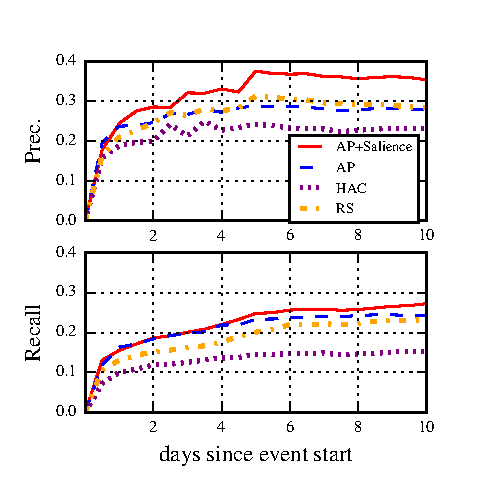
\includegraphics[]{strmsum/figures/rouge-time.eps}};
        \node[draw=white,fill=white,text width=1.05cm] at (2.20,1.55) {};
        \node[draw=white,fill=white,inner sep=0pt,text width=1.05cm] at (2.20,1.60) {\tiny SAP};
        \node[draw=white,fill=white,text width=1.05cm] at (2.20,1.30) {};
        \node[draw=white,fill=white,text width=1.05cm] at (2.20,0.95) {};
        \node[draw=white,fill=white,text width=1.05cm] at (2.20,0.55) {};

        \node[draw=white,fill=white,inner sep=0pt,text width=1.05cm] at (2.20,1.25) {\tiny AP};
        \node[draw=white,fill=white,inner sep=0pt,text width=1.05cm] at (2.20,0.90) {\tiny HAC};
        \node[draw=white,fill=white,inner sep=0pt,text width=1.05cm] at (2.20,0.55) {\tiny RS};
    \end{tikzpicture}
    \caption{System \textsc{Rouge-1} performance over time.}
\label{fig:trouge}
%\vspace{-14pt}
\end{figure}




\paragraph{\rouge} 
\autoref{tab:rouge} shows our results for system output samples against the
full summary of nuggets using \rouge. SAP improves over the individual
component systems, i.e. affinity propagation only (AP) or salience prediction
only (RS), suggesting the combination of these two components is beneficial.
This improvement is statistically significant for $\rouge-1$ and $\rouge-2$
precision, recall, and F-measures at the $\alpha = .01$ level using the
Wilcoxon signed-rank test.  The full system or the individual components AP and
RS also outperform the alternative clustering method HAC. 

SAP maintains its performance above the baselines over time as well.
\autoref{fig:trouge} shows the \rouge-1 scores over time. We show the
difference in unigram precision (bigram precision is not shown but it follows
similar curve). Within the initial days of the event, SAP is able to take the
lead over the other systems in ngram precision. The SAP model is better able to
find salient updates earlier on; for news and crisis informatics, this is an
especially important quality of the model.  Moreover, the SAP's recall is not
diminished by the high precision and remains competitive with \textsc{AP}.
Over time SAP's recall also begins to pull away, while the other models begin
to plateau.

\begin{figure}[t]
    \centering
\begin{tikzpicture}
  \node at (0,0) {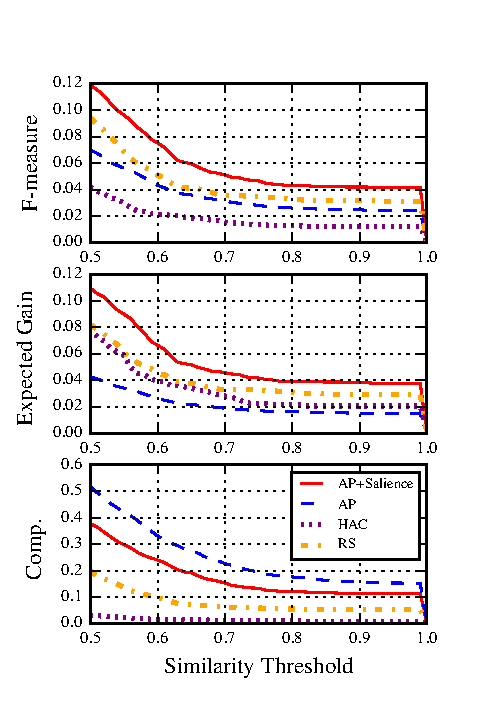
\includegraphics[]{strmsum/figures/nuggets-metrics2.eps}};
    \draw[rectangle,fill=white,draw=white] (2.85,-3.35) rectangle (1.5,-2.1); 
\node[anchor=north west, align=left,font=\tiny,inner sep=0] at (1.5,-2.1) {SAP\\[2.9pt] AP\\[2.9pt] HAC\\[2.9pt] RS};
\end{tikzpicture}
\caption{Expected Gain and Comprehensiveness performance.}
\label{fig:nperf}
%\vspace{-12pt}
\end{figure}




\paragraph{Expected Gain and Comprehensiveness}
\autoref{fig:nperf} shows the expected gain across a range of similarity
thresholds, where thresholds closer to 1 are more conservative estimates.  The
ranking of the systems remains constant across the sweep with \textsc{SAP}
beating all baseline systems. Predicting salience in general is helpful for
keeping a summary on topic as the \textsc{RS} approach outperforms the
clustering only approaches on expected gain.

When looking at the comprehensiveness of the summaries \textsc{AP} outperforms
\textsc{SAP}. The compromise encoded in the \textsc{SAP} objective function,
between being representative and being salient, is seen clearly here where the
performance of the \textsc{SAP} methods is lower bounded by the salience
focused \textsc{RS} system and upper bounded by the clustering only \textsc{AP}
system. Overall, \textsc{SAP} achieves the best balance of these two metrics.

\subsection{Feature Ablation}
\begin{table}[h]
\centering
% centering table
\begin{tabular}{l D{.}{.}{3} D{.}{.}{3} D{.}{.}{3} D{.}{.}{3} D{.}{.}{3} D{.}{.}{3}}
    \toprule
% creating 10 columns
    & \multicolumn{3}{c}{\textsc{Rouge}-1}
    & \multicolumn{3}{c}{\textsc{Rouge}-2}\\
    \cmidrule(lr){2-4} \cmidrule(lr){5-7}
    Model & \multicolumn{1}{c}{Recall} & \multicolumn{1}{c}{Prec.} & \multicolumn{1}{c}{$\textrm{F}_1$} &
\multicolumn{1}{c}{Recall} & \multicolumn{1}{c}{Prec.} & \multicolumn{1}{c}{$\textrm{F}_1$} \\
\midrule
Full System & 0.282 & 0.344 & 0.306 & 0.045 & 0.056 & 0.049\\
No Basic    & 0.263 & 0.380 \rlap{\textsuperscript{$\dagger$}}  & 0.294 & 0.046 & 0.068 \rlap{\textsuperscript{$\dagger\dagger$}} & 0.051 \rlap{\textsuperscript{$\dagger$}}\\
No LM       & 0.223 \rlap{\textsuperscript{$\dagger$}} & 0.361 & 0.254 \rlap{\textsuperscript{$\dagger$}} & 0.033 \rlap{\textsuperscript{$\dagger$}} & 0.056 & 0.038 \rlap{\textsuperscript{$\dagger$}} \\
No Time  & 0.297 \rlap{\textsuperscript{$\dagger$}} & 0.367 \rlap{\textsuperscript{$\dagger\dagger$}} & 0.322 \rlap{\textsuperscript{$\dagger$}} & 0.052 \rlap{\textsuperscript{$\dagger\dagger$}} & 0.064 \rlap{\textsuperscript{$\dagger\dagger$}} & 0.056 \rlap{\textsuperscript{$\dagger\dagger$}} \\ 
No Geo   & 0.232 \rlap{\textsuperscript{$\dagger\dagger$}} & 0.381 & 0.265 \rlap{\textsuperscript{$\dagger$}} & 0.037 \rlap{\textsuperscript{$\dagger$}} & 0.065 & 0.042 \\  
No Query & 0.251 & 0.377 & 0.280 & 0.043 & 0.068 \rlap{\textsuperscript{$\dagger$}} & 0.048 \\
\bottomrule
\end{tabular}
\caption{Feature ablation \textsc{Rouge} performance. 
    $\dagger$ indicates statistically significant difference from 
full model at the $\alpha=.05$ level.
    $\dagger\dagger$ indicates statistically significant difference from 
full model at the $\alpha=.01$ level.
    } % title name of the table
\label{tab:farouge}
\end{table}








\autoref{tab:farouge} shows the results of our feature ablation tests.
Removing the language models yields a statistically significant drop in both
ngram recall and F-measure. 

Removing the language model and geographic relevance features leads to a
statistically significant drop in \rouge-1 F1 scores. Unfortunately, this is
not the case for the temporal relevance features. We surmise that these
features are too strongly correlated with each other, i.e. the differences in
TF-IDF between hours are definitely not i.i.d.  variables. 

Interestingly, removing the basic features leads to an increase in both unigram
and bigram precision; in the bigram case this is enough to cause a
statistically significant increase in F-measure over the full model. In other
words, the generic features actually lead to an inferior model when we can
incorporate more appropriate domain specific features.  This result perhaps
echoes the claim of \cite{jones1999} that generic approaches to summarization
are unlikely to produce truly useful summaries.

\section{Learning-to-Search (L2S) Summarizer}

While our previous summarization model proved reasonably capable of summarizing
events over time, by processing the stream in hourly batches it was limited in
its ability to respond quickly to unfolding events. One reason for this
limitation is an implicit assumption in that model, and most multi-document
summarization models, that frequency of a unit of text is a proxy for its
salience. In retrospective summarization of static document collections, this
is a reasonable assumption, and has been exploited successfully in various
ways: TF-IDF term weightings, document language models derived from frequency,
and random-walks on sentence-graphs  whose edges are determined by frequently
co-occurrring terms
\citep{lin2000,radev2000,erkan2004,mihalcea2004,nenkova2005,daume2006}. 

In the streaming setting these proxy features are constantly evolving. There
may be fallow periods in an event where nothing happens and then sudden bursts
of activity. The behavior of SAP is unsuited for this, in that it is run every
hour regardless.  In the SAP model, by collecting an hour's worth of documents
and performing a salience-biased clustering, we try to walk the line between
using clustering, where the frequency of like text units are effectively votes
for the most salient unit, and predictions about salience from our regression
model, which makes more use of the semantics of the query event and text unit
under analysis.  However, as we showed in the feature ablation, incorporating
time-based frequency features made the model worse. While we are able to
incorporate salience estimate successfully into the summarization model with
SAP, we have yet to successfully provide a learning-based of model the entire
summarization process.

In this section, we attempt to overcome these limitations, removing the
clustering component from the update selection, and develop a fully online
streaming summarization model, one that learns to make extraction decisions
immediately upon seeing the next sentence from $\sentstream$, using features
derived from the entire observed document stream, the state of the current
update summary, and the model's prior extraction decisions.  To that end, we
present a novel streaming-document summarization system based on sequential
decision making.  Specifically, we adopt the ``learning to search'' approach, a
technique which adapts methods from reinforcement learning for structured
prediction problems \citep{daume2009,ross2010}.  In this framework, we cast
streaming summarization as a form of greedy search and train our system to
imitate the behavior of an oracle summarization system.  Effectively, we train
a linear classifier to predict when to extract a sentence $\ssent \in
\sentstream$ using features of the sentence, query, previous summary updates,
and other aggregate statistics collected from the stream up to the current time
$\systs_t$. 

As in the previous section,  we report both the TREC 2015 Temporal
Summarization shared-task manual evaluation as well as our own independent
automatic evaluation.  In our evaluation we demonstrate a 28.3\% improvement in
summary $\harm_\latency(\updateSummary)$ and a 43.8\% improvement in
time-sensitive $\harm_\latency(\updateSummary)$ metrics against several
state-of-the-art baselines.  In shared-task evaluation of our system at TREC
2015, where we were the second-best performing team in the main evaluation, and
top system for a secondary evaluation run on a pre-filtered, highly relevant
document stream.

\subsection{Stream Summarization as Sequential Decision Making}

We could na{\"i}vely treat the stream summarization problem as classification
and predict which sentences to extract or skip. However, this would make it
difficult to take advantage of many features (e.g. sentence novelty with regard
to previous updates).  What is more concerning, however, is that the
classification objective for this task is somewhat ill-defined: successfully
predicting extract on one sentence changes the true label (from extract to
skip) for sentences that contain the same information but occur later in the
stream.
 
In this work, we pose stream summarization as a greedy search over a binary
branching tree where each level corresponds to a position in the stream (see
\autoref{fig:search}).  The height of the tree corresponds to the length of
stream.  A path through the tree is determined by the system extract and skip
decisions.
 
\begin{figure}
  \center
\fbox{\begin{tikzpicture}[
    state/.style={fill,draw,circle,minimum height=1mm,inner sep=0.0mm},
    policy/.style={line width=0.5mm,circle,minimum height=2.25mm,
                   inner sep=0.0mm},
    rollin/.style={policy,draw=green},
    rolloutA/.style={policy,draw=purple},
    rolloutB/.style={policy,draw=orange},
    action/.style={line width=0.75mm},
    rolloutAline/.style={action,draw=purple},
    rolloutBline/.style={action,draw=orange},
    rollinline/.style={action,draw=green},
]

\def\WIDTH{0.32};
\def\TH{6}

\node at (5,\TH + 1.6) {\large \textbf{Search Space}};
\node at (-0.1,\TH + 1.6) {\large \textbf{Sentence Stream}};
\node at (-0.1,\TH + 1) 
    {$\sentstream_{\poestart:\poestop}$};
\node at (-0.1,\TH + 0.9) 
    {\uline{$\phantom{\sentstream^{(\query)}_{\timestamp_\starttok:\timestamp_\stoptok}}$}};

\foreach \n [
    % compute the number of nodes \numnodes from the line \n
    evaluate=\n as \numnodes using int(2^(\TH-1)/(2^(\n-1)), 
    % compute the (\n-1)th line.
    evaluate=\n as \nmo using int(\n-1)
] in {1,...,\TH} {

    
    \ifthenelse{\n=6}{}{
        \node at (-0.1,\TH - \n + 1) {$\ssent_\n$};
    }
    
    \foreach \x [
        evaluate=\x as \xcoord using \x*\WIDTH*2^(\n-1)-\WIDTH*2^(\n-1)/2,
        evaluate=\x as \lc using int(2*\x - 1),
        evaluate=\x as \rc using int(2*\x)
    ] in {1,...,\numnodes} {

        \node[state] (a\n\x) at (\xcoord,\n) {};
        \ifthenelse{\nmo=0}{}{
                \draw (a\n\x.south west) -- (a\nmo\lc.north);
                \draw (a\n\x.south east) -- (a\nmo\rc.north);
        }
    }

}
\node[rollin] (ri1) at (a61) {};
\node[rollin] (ri2) at (a52) {};
\node[rollin] (ri3) at (a43) {};
\node[rollin] (ri4) at (a35) {};
\node[rollin] (ri5) at (a29) {};
\node[rollin] (ri6) at (a118) {};

\foreach \n [
    % compute the (\n-1)th line.
    evaluate=\n as \nmo using int(\n-1)
] in {2,...,6} {
    \draw[rollinline] (ri\nmo.south) -- (ri\n.north);
};

\node[rotate=-20] at ($(ri1)!0.5!(ri2)+(0,0.25)$) {\tiny extract};
\node[rotate=32] at ($(ri2)!0.5!(ri3)+(0,0.25)$) {\tiny skip};
\node[rotate=45] at ($(ri3)!0.5!(ri4)+(-0.25,0.25)$) {\tiny skip};
\node[rotate=58] at ($(ri4)!0.5!(ri5)+(-0.25,0.25)$) {\tiny skip};
\node[rotate=-76] at ($(ri5)!0.5!(ri6)+(+0.25,0.0)$) {\tiny extract};

\node at ($(ri1)+(0.25,0.25)$) {$\state_1$}; 
\node at ($(ri2)+(0.25,0.25)$) {$\state_2$}; 
\node at ($(ri3)+(-0.25,0.25)$) {$\state_3$}; 
\node at ($(ri4)+(-0.25,0.25)$) {$\state_4$}; 
\node at ($(ri5)+(+0.25,0.25)$) {$\state_5$}; 
\node at ($(ri6)+(-0.25,-.25)$) {$\state_6$}; 
%\draw[rollinline] (ri2.west) -- (ri3.north);
\end{tikzpicture}}


\caption{Search space for a stream of 5 sentences.  Left branches skip the
current sentence.  Right branches indicate extracting the current sentence as
an update.  The path in green corresponds to one trajectory through this space
consisting of extracting sentence $\ssent_1$, then skipping sentences
$\ssent_2,\ldots,\ssent_4$ and extracting sentence $\ssent_5$.}
  \label{fig:search}
\end{figure}



When treated as a sequential decision making problem, our task reduces to
defining a policy for selecting a sentence based on its features as well as the
features of its ancestors (i.e., all of the observed sentences and previous
extraction decisions).  The union of these features represents the current
state in the decision making process. 

The feature representation provides state abstraction both within a given
query's search tree as well as to states in other queries' search trees, and
also allows for complex interactions between the current update summary,
candidate sentences, and stream dynamics unlike the classification approach.

In order to learn an effective policy for a query $\query$, we can take one of
several approaches.  We could use a simulator to provide feedback to a
reinforcement learning algorithm.  Alternatively, if provided access to an
evaluation algorithm at training time, we can simulate (approximately) optimal
decisions. That is, using the training data, we can define an \emph{oracle
policy} that is able to omnisciently determine which sentences to extract and
which to skip.  Moreover, it can make these determinations by starting at the
root or at an arbitrary node in the tree, allowing us to observe optimal
performance in states unlikely to be reached by the oracle.  We adopt
\textit{locally optimal learning to search} to learn our model from the oracle
policy \citep{chang2015}.  

\subsection{Policy-based Stream Summarization}

In the induced search problem, each search state $\state_t \in \states$
corresponds to observing the first $t$ sentences in the stream $\left[
\ssent_1,\ldots, \ssent_t \right] \subset \sentstream$ and a sequence of $t-1$
actions $\bsal_1, \ldots, \bsal_{t-1}$.  For each state $\state_t \in \states$,
the set of actions is $\bsal_t \in \{0,1\}$ with $\bsal_t =1$ indicating we
extract the $t$-th sentence and add it to our update summary, and $\bsal_t = 0$
indicating we skip it. For simplicity of exposition, we assume a fixed length
stream of size $T$ but this is not strictly necessary. 

\begin{algorithm}[t]
  \RestyleAlgo{boxruled}
  \LinesNumbered
  \KwIn{
    query string $\query$, 
    query category $\category$, 
    stream $\sentstream$, 
    period of interest ($\poestart$, $\poestop$), 
    summarization policy $\policy$}
  \KwOut{update summary $\updateSummary$}
  $\updateSummary \gets \{\}$

\For{$\ssent_t \in \sentstream_{\poestart:\poestop}$}{
    $\state_t \gets (\ssent_1,\ldots,\ssent_t, \bsal_1,\ldots,\bsal_{t-1},
                     \query,\category)$\\
    $\bsal_t \gets \policy(\state_t)$\\
    \If{$\bsal_t = 1$}{
        $\updateSummary \gets \updateSummary \cup \left\{\left(\ssent_t, \sentts_t \right) \right\} $
        }
    }
  \caption{Policy-based Stream Summarization} 
  \label{alg:policysum}
\end{algorithm}




A policy, $\policy : \states \rightarrow \{0,1\}$, is a mapping from states to
an extraction decision. Given a policy, the policy-based stream summarization
algorithm (\autoref{alg:policysum}) is trivial, iterating sequentially over
sentences in the stream, and adding each sentence to the update summary if it
is the current action determined by $\policy$.  In practice, we use a linear
cost-sensitive classifier to implement $\policy_\params$, with \[ \bsal_t =
\policy_\params(\state_t) = \argmin_{\bsal \in \{0,1\}} \Feat(\state_t,
\bsal)\cdot \params_\bsal\] where we encode each state-potential action pair
$(\state_t,\bsal)$ as a $d$-dimensional feature vector  $\Feat(\state_t, \bsal)
\in \mathbb{R}^d$ and $\params_0, \params_1 \in \reals^{d}$ are learned
parameters.  Note that $\Feat(\state_t,\bsal)\cdot \params_\bsal$ is a linear
regression to predict the cost, which we define shortly, associated with taking
action $\bsal$ in state $\state_t$. Given estimates of our two available
actions, extracting a sentence or ignoring it, our policy $\policy_\policy$
selects the action with minimum cost.

Before we can define cost more concretely, we must first introduce some
additional notation and concepts.  For a given sequence of states
$\state_1,\ldots,\state_T$ explored by a policy $\policy$, let $\bsals=
\left[\bsal_1,\ldots,\bsal_T\right]$ be the associated sequence of actions
taken by $\policy$, i.e. $\bsal_t = \policy(\state_t)$.  A loss function,
$\lossfunc : \{0,1\}^T \rightarrow \reals$, measures the quality of an action
sequence $\bsals$. In our present case this might be the negative
\textsc{Rouge} score of the update summary that results from $\bsals$ or some
other relevant measure of performance. 

Let $\policy$ be a policy, $\state_1,\ldots,\state_T$ a sequence of states
explored by $\policy$, and the corresponding action sequence $\bsals$. We also
define a second policy, $\rolloutpolicy$, which we call the roll-out policy and
which may or may not be distinct from $\policy$.  For any state $\state_t$ we
can then define two additional action sequences,
\[
    \roaseqt = \left[
        \bsal_1, 
        \ldots, 
        \bsal_{t-1},
        \hat{\bsal}_t,
        \roat_{t+1}, 
        \ldots, 
        \roat_{T}, 
    \right] \quad \forall \predbsal_t \in \{0,1\} 
\] 
where $\roaseqt$ is the sequence of actions that result from following
$\policy$ on the first $t-1$ states, taking action $\predbsal_t$ at state
$\state_t$ and then following $\rolloutpolicy$ on the remaining $T - t$ states.
That is, for $k > t$, $\roa_{k} = \rolloutpolicy(\state^\prime_k)$, where
$\state^\prime_k$ is the state that results from taking action $\predbsal_t$ in
$\state_t$ and following $\rolloutpolicy$ on a sequence of states
$\state^\prime_{t+1}, \ldots, \state^\prime_k$. The loss, $\lossfunc\left(
\roaseq{t}{0} \right)$, then reflects the evaluation measure for an update
summary where sentence $\ssent_t$ was not extracted, and $\rolloutpolicy$
completed the summary of the stream. Similarly, $\lossfunc\left( \roaseq{t}{1}
\right)$ reflects the evaluation measure for an update summary where sentence
$\ssent_t$ was extracted, and $\rolloutpolicy$ completed the summary of the
stream. 
 
We can now define the cost of an action $\bsal$ in state $\state_t$ as 
\[ 
    \cost(\state_t, \bsal) = 
        \lossfunc\left(\roaseq{t}{\bsal}   \right) 
            - \min_{\bsal^\prime \in \{0,1\} }
                \lossfunc\left( \roaseq{t}{\bsal^\prime} \right).
\]
Note that the cost is also a function of $\rolloutpolicy$, which determines how
the action sequence is completed after $\state_t$.  The costs connect the
overall summary loss $\lossfunc\left(\roaseqt\right)$ to a particular action in
$\state_t$ that builds the summary.  We depict an example of the cost
computation in \autoref{fig:rollouts}.  We discuss how to collect costs and
learn $\params_0$ and $\params_1$ such that they are good estimators of cost in
the next section.


\begin{figure}[p]
    \fbox{\resizebox{\textwidth}{!}{\begin{tikzpicture}[
    state/.style={fill,draw,circle,minimum height=1mm,inner sep=0.0mm},
    policy/.style={line width=0.5mm,circle,minimum height=2.25mm,
                   inner sep=0.0mm},
    rollin/.style={policy,draw=green},
    rolloutA/.style={policy,draw=purple},
    rolloutB/.style={policy,draw=orange},
    action/.style={line width=0.75mm},
    rolloutAline/.style={action,draw=purple},
    rolloutBline/.style={action,draw=orange},
    rollinline/.style={action,draw=green},
]

\def\WIDTH{0.32};
\def\TH{6}

\node at (0.1,\TH + 1.6) {\large \textbf{Sentence Stream}};
\node at (5,\TH + 1.6) {\large \textbf{Search Space}};
\node at (13,\TH + 1.6) {\large \textbf{Roll-out Action Sequences}};
\node at (-0.1,\TH + 1) 
    {$\sentstream_{\poestart:\poestop}$};
\node at (-0.1 ,\TH + 0.9) 
    {\uline{$\phantom{\sentstream^{(\query)}_{\timestamp_\starttok:\timestamp_\stoptok}}$}};

\foreach \n [
    % compute the number of nodes \numnodes from the line \n
    evaluate=\n as \numnodes using int(2^(\TH-1)/(2^(\n-1)), 
    % compute the (\n-1)th line.
    evaluate=\n as \nmo using int(\n-1)
] in {1,...,\TH} {

    
    \ifthenelse{\n=6}{}{
        \node at (-0.1,\TH - \n + 1) {$\ssent_\n$};
    }
    
    \foreach \x [
        evaluate=\x as \xcoord using \x*\WIDTH*2^(\n-1)-\WIDTH*2^(\n-1)/2,
        evaluate=\x as \lc using int(2*\x - 1),
        evaluate=\x as \rc using int(2*\x)
    ] in {1,...,\numnodes} {

        \node[state] (a\n\x) at (\xcoord,\n) {};
        \ifthenelse{\nmo=0}{}{
            \ifthenelse{\n=4 \AND \x=3}{
                \draw[draw=blue,dashed,line width=0.5mm] 
                    (a\n\x.south west) -- (a\nmo\lc.north);
                \draw[draw=red,dashed,line width=0.5mm] 
                    (a\n\x.south east) -- (a\nmo\rc.north);
            }{
                \draw (a\n\x.south west) -- (a\nmo\lc.north);
                \draw (a\n\x.south east) -- (a\nmo\rc.north);
            }
        }
    }

}

\node[rollin] (ri1) at (a61) {};
\node[rollin] (ri2) at (a52) {};
\node[rollin] (ri3) at (a43) {};
\draw[rollinline] (ri1.east) -- (ri2.north);
\draw[rollinline] (ri2.west) -- (ri3.north);
\node[rotate=-20] at ($(ri1)!0.5!(ri2)+(0,0.25)$) {\tiny extract};
\node[rotate=32] at ($(ri2)!0.5!(ri3)+(0,0.25)$) {\tiny skip};
\node[rolloutA] (roa4) at (a35) {};
\node[rolloutA] (roa5) at (a210) {};
\node[rolloutA] (roa6) at (a119) {};
\node[rolloutB] (rob4) at (a36) {};
\node[rolloutB] (rob5) at (a211) {};
\node[rolloutB] (rob6) at (a121) {};
\node at ($(ri1)+(0.25,0.25)$) {$\state_1$}; 
\node at ($(ri2)+(0.25,0.25)$) {$\state_2$}; 
\node at ($(ri3)+(-0.25,0.25)$) {$\state_3$}; 
\node[rotate=-73.5] at ($(roa4)!0.5!(roa5)+(0.25,0)$) {\tiny extract};
\node[rotate=84] at ($(roa5)!0.5!(roa6)+(-0.25,0)$) {\tiny skip};
\node[rotate=73.5] at ($(rob4)!0.5!(rob5)+(-.25,0)$) {\tiny skip};
\node[rotate=84] at ($(rob5)!0.5!(rob6)+(-0.25,0)$) {\tiny skip};
\draw[rolloutAline] (roa4.south east) -- (roa5.north);
\draw[rolloutAline] (roa5.south west) -- (roa6.north);
\draw[rolloutBline] (rob4.south west) -- (rob5.north);
\draw[rolloutBline] (rob5.south west) -- (rob6.north);

\def\COffset{36*\WIDTH}
\node at (\COffset, \TH+0.5) {$\uline{\roaseq{3}{0}\phantom{= 1}}$};
\node at (\COffset + 3, \TH+0.5) {$\uline{\roaseq{3}{1}\phantom{= 1}}$};

\def\SPACE{\phantom{\left(t,\hat{\bsal},\rolloutpolicy\right)}}
\foreach \ya/\yb [count=\t from 1] in {1/1, 0/0, 0/1, 1/0, 0/0} {
    \ifthenelse{
        \t<3
    }{ 
        \node (ya\t) at (\COffset, \TH-\t + 0.5) 
            {$\bsal^{\SPACE}_\t=\ya$};
        \node (yb\t) at (\COffset+3, \TH-\t + 0.5) 
            {$\bsal^{\SPACE}_\t=\yb$};
    }{
        \ifthenelse{
            \t=3                
        }{
            \node (ya\t) at (\COffset, \TH-\t + 0.5) 
                {$\predbsal^{\SPACE}_\t=\ya$};
            \node (yb\t) at (\COffset+3, \TH-\t + 0.5) 
                {$\predbsal^{\SPACE}_\t=\yb$};
        }{
            \node (ya\t) at (\COffset, \TH-\t + 0.5) 
                {$\roa{3}{0}_\t=\ya$};
            \node (yb\t) at (\COffset+3, \TH-\t + 0.5) 
                {$\roa{3}{1}_\t=\yb$};

        }
    }
}

\draw[draw=green,fill=green!20,line width=0.25mm] 
    (ya1.north west) rectangle (ya2.south east);
\draw[draw=green,fill=green!20,line width=0.25mm] 
    (yb1.north west) rectangle (yb2.south east);
\draw[draw=blue,fill=blue!20,line width=0.25mm] 
    (ya3.north west) rectangle (ya3.south east);
\draw[draw=red,fill=red!20,line width=0.25mm] 
    (yb3.north west) rectangle (yb3.south east);
\draw[draw=purple,fill=purple!20,line width=0.25mm] 
    (ya4.north west) rectangle (ya5.south east);
\draw[draw=orange,fill=orange!20,line width=0.25mm] 
    (yb4.north west) rectangle (yb5.south east);


%\node at (by1) {$\bsal_1^{\phantom{\left(3,0,\rolloutpolicy\right)}}=1$};
%\node at (by2) {$\bsal_2^{\phantom{\left(3,0,\rolloutpolicy\right)}}=0$};
%\node at (by3) {$\hat{\bsal}_3^{\phantom{\left(3,0,\rolloutpolicy\right)}}=1$};
%\node at (by4) {$\bsal^{\left(3,1,\rolloutpolicy\right)}_4=0$};
%\node at (by5) {$\bsal^{\left(3,1,\rolloutpolicy\right)}_5=0$};
%
%\node (ay1) at (36*\WIDTH, \TH-1+0.5) {$\bsal_1^{\phantom{\left(3,0,\rolloutpolicy\right)}}=1$};
%\node (ay2) at (36*\WIDTH, \TH-2+0.5) {$\bsal_2^{\phantom{\left(3,0,\rolloutpolicy\right)}}=0$};
%\node (ay3) at (36*\WIDTH, \TH-3+0.5) {$\hat{\bsal}_3^{\phantom{\left(3,0,\rolloutpolicy\right)}}=0$};
%\node (ay4) at (36*\WIDTH, \TH-4+0.5) {$\bsal^{\left(3,0,\rolloutpolicy\right)}_4=1$};
%\node (ay5) at (36*\WIDTH, \TH-5+0.5) {$\bsal^{\left(3,0,\rolloutpolicy\right)}_5=0$};

\foreach \ya/\yb [count=\t from 1] in {1/1, 0/0, 0/1, 1/0, 0/0} {
    \ifthenelse{
        \t<3
    }{ 
        \node (ya\t) at (\COffset, \TH-\t + 0.5) 
            {$\bsal^{\SPACE}_\t=\ya$};
        \node (yb\t) at (\COffset+3, \TH-\t + 0.5) 
            {$\bsal^{\SPACE}_\t=\yb$};
    }{
        \ifthenelse{
            \t=3                
        }{
            \node (ya\t) at (\COffset, \TH-\t + 0.5) 
                {$\predbsal^{\SPACE}_\t=\ya$};
            \node (yb\t) at (\COffset+3, \TH-\t + 0.5) 
                {$\predbsal^{\SPACE}_\t=\yb$};
        }{
            \node (ya\t) at (\COffset, \TH-\t + 0.5) 
                {$\roa{3}{0}_\t=\ya$};
            \node (yb\t) at (\COffset+3, \TH-\t + 0.5) 
                {$\roa{3}{1}_\t=\yb$};

        }
    }
}

\node[anchor=north west,align=left,text width=17.0cm] at (-1.5,0) {
\textbf{Computing Costs  $\cost(\state_3,0)$ and $\cost(\state_3,1)$}\\

~\\

\textbf{Step 1. Roll-in to $\state_3$ with policy $\policy$.}\\
Use policy $\policy$ to explore to state $\state_3$, shown in {\color{green}green} in the search space above.\\~\\  
\textbf{Step 2. Roll-out with $\rolloutpolicy$ to create action sequences
$\roaseq{3}{0}$ and $\roaseq{3}{1}$.}\\
For each action $\predbsal_3 \in \{0,1\},$ use $\rolloutpolicy$ to 
complete the roll-outs after having made action $\predbsal_3$ in state $\state_3$ (shown in {\color{purple}purple} and {\color{orange}orange} respectively) and create
alternative action sequences $\roaseq{3}{0}$ and $\roaseq{3}{1}$ (shown on 
the right).\\~\\
\textbf{Step 3. Compute losses.}\\
After completing the roll-outs, compute losses 
$\lossfunc\left(\roaseq{3}{0}\right)$ and $\lossfunc\left(\roaseq{3}{1}\right)$.\\~\\
\textbf{Step 4. Compute costs.}\\
Compute 
\[\cost(\state_3,0) = \lossfunc\left( \roaseq{3}{0} \right) - \min_{\bsal^\prime \in \{0,1\}} \lossfunc\left( \roaseq{3}{\bsal^\prime} \right)\]
and  
\[\cost(\state_3,1) = \lossfunc\left( \roaseq{3}{1} \right) - \min_{\bsal^\prime \in \{0,1\}} \lossfunc\left( \roaseq{3}{\bsal^\prime} \right).\]

};

\end{tikzpicture}}}
\caption{Example of computing costs of actions at $\state_3$ using roll-out
policy $\rolloutpolicy$.}
\label{fig:rollouts}
\end{figure}


\subsection{The Locally-Optimal Learning-to-Search Algorithm}
\label{sec:algorithm}

In a perfect world, we would have a training set of state-action pairs,
$(\state_t,\bsal_t)$, and their associated costs $\cost(\state_t, \bsal_t)$,
drawn from a distribution of states similar to the one our final learned policy
would produce.  With these states, actions, and costs in hand we could fit two
linear regressions, one for estimating the cost of extract actions and one for
skip actions from a given state's feature representation; we would immediately
have a suitable stream summarization policy. Unfortunately, we do not have a
reasonable distribution of state-action pairs let alone the associated costs.
Instead we turn to the locally-optimal learning-to-search (LOLS) algorithm
\citep{chang2015}, presented in \autoref{fig:lols}, to iteratively refine our
learned policy as it attempts to follow an oracle policy. 

At a high level, we begin with an initially random learned policy.  We leverage
a heuristic oracle stream summarizer and our learned policy to collect
state-action pairs and their costs from the training set query-streams, with
our learned policy gradually learning to imitate the heuristic oracle. Using
both the oracle and learned policy to sample state-action-cost triples is
beneficial as it exposes the learned policy to a mix of states it is likely to
encounter when following its own actions, but also state-actions of the better
performing reference summarizer. Exploring with the learned policy alone may be
less optimal because it may overestimate the costs of good decisions since its
roll-outs at the beginning of training are likely to be quite bad.  Exploring
with only the oracle would also be harmful as the distribution of states it
produces will reflect an optimistic level of performance from learned policy
that it will not be able to match in practice.

\subsubsection{Oracle Policy}

For a given policy $\policy$, training query $\query$, stream $\sentstream$,
and reference summary $\snuggets$, we construct a greedy heuristic oracle
policy $\oracle_\query$.  Let $\updateSummary_t$ be the update summary at state
$\state_t$ reached by $\policy$. Additionally, let
\[
\snuggets_{\denotes{\updateSummary_t}} = 
\left\{\snugget_i \Bigg\vert
        \left(\snugget_i,\nts_i\right) \in \snuggets,
         \exists \left(\supdate_j, \uts_j\right) \in \updateSummary_t : \denotes{\snugget_i} \in
        \denotes{\supdate_j}
       \right\}
\]
be the set of nuggets covered by the updates in the update summary at
$\state_t$, and let
\[
\snuggets_{\denotes{\ssent_t}} = 
\left\{\snugget_i \Bigg\vert
        \left(\snugget_i,\nts_i\right) \in \snuggets,
        \denotes{\snugget_i} \in
        \denotes{\ssent_t}
       \right\}
\]
be the set of nuggets covered by $\ssent_t$.  The oracle $\oracle_\query$,
which has clairvoyant knowledge of these sets, performs the following actions
given a state $\state_t$,
\[
    \oracle_\query(\state_t) = \begin{cases} 
        1 & \textrm{if }  
        \exists \snugget : \snugget \in \snuggets_{\denotes{\ssent_t}} \wedge 
   \snugget \not\in \snuggets_{\denotes{\updateSummary_t} }
     \\
     0 & \textrm{otherwise.} \end{cases}
\]
In other words, the oracle policy will extract $\ssent_t$ at state $\state_t$
if $\ssent_t$ covers any nuggets not yet covered by updates in the update
summary $\updateSummary_t$. We describe how we obtain comprehensive
nugget/sentence covers, i.e. the sets $\snuggets_{\denotes{\ssent_t}}$ in
\autoref{sec:reljudge}.

\subsubsection{Loss Function}
We design our loss function to penalize policies that  over- or under-generate.
Let $\state_1, \ldots, \state_T$ be the sequence of states associated with the
action sequence $\bsals$.  We define the loss of a sequence as 
\begin{align*}
  \lossfunc(\bsals) = 1 - 2 \times 
    \frac{ \bsals^\T \bsals^* }{ \sum^T_{i=1} \bsal_i + \sum^T_{j=1}\bsal_j^* }
\end{align*}
where $\bsals^* = \left[\bsal_1^*,\ldots, \bsal_T^* \right]$ is a reference
sequence of consisting of the one-step optimal deviations under the oracle
policy, i.e. $\bsal_t^* = \oracle_\query(\state_t)$.

Note that $\lossfunc$ is the complement of the Dice coefficient.  This
encourages not only local agreement between policies (the numerator of the
second term) but that the learned and oracle policy should generate roughly the
same number of updates (the denominator in the second term).

\begin{algorithm}[t]
  \RestyleAlgo{boxruled}
  \LinesNumbered
  \KwIn{training dataset of query-relevant streams and oracle policies $\{\sentstream_\query, \oracle_{\query} \}_{\query\in\queries}$, number of 
        training epochs $N$, learning rate $\lambda$, and a mixture parameter $\beta \in (0,1)$ for 
        selecting a roll-out policy.}
  \KwOut{learned summarization policy $\policy_\params$}
  Initialize $\params$ \label{alg:lolsinit}\\
  \For{$n \gets 1,2,\ldots, N$}{
    \For{$\query \in \queries$}{
      $\Train \gets \{\}$\\    
      \For{$t \in \{1,\ldots,T \}$}{
        Roll-in by executing $\policy_\params$ on $\sentstream_\query$ for $t-1$ rounds and reach state $s_t$. \label{alg:lolsrollin} \\
        \For{$y \in \{0,1\}$}{
            Pick roll-out policy $\rolloutpolicy \gets \begin{cases} \oracle_{\query} & \textrm{with probability $\beta$}\\ \policy_\params & \textrm{with probability $1 -\beta$.}\end{cases}$. \label{alg:lolsrollout}\\
            Compute roll-out action sequence $\bsals^{(t,\bsal,\rolloutpolicy)}$. \label{alg:lolsaction}\\
        }      
        \For{$y \in \{0,1\}$}{
            $\cost(\state_t, \bsal) \gets \ell\left(\bsals^{\left(t,\bsal,\rolloutpolicy\right)}\right) - \min_{\bsal^\prime \in \{0,1\}} \ell\left(\bsals^{\left(t,\bsal^\prime,\rolloutpolicy\right)}\right) $ \label{alg:lolscoststart}  \\
            $\Train \gets \Train \cup \left\{\left( \Feat(\state_t,\bsal),
            c(\state_t, \bsal), \bsal\right)\right\}$ \label{alg:lolscoststop}  }}
    \For{$\left(\Feat(\state,\bsal),
            c(\state, \bsal), \bsal\right) \in \Train$ \label{alg:lolsmsestart} }{
        $\params_\bsal \gets \params_\bsal - \lambda \nabla_{\params_\bsal}(c(\state, \bsal) - \Feat(\state,\bsal)\cdot \params_\bsal  )^2$ \label{alg:lolsmsestop}
}
}}
  \KwResult{$\policy_\params$}
  \caption{Locally Optimal Learning-to-Search for Stream Summarization} 
  \label{fig:lols}
\end{algorithm}




\subsubsection{Learning with LOLS}

We now step through the LOLS algorithm in detail.  Our initial policy
parameters $\params_0$ and $\params_1$ are randomly initialized
(\hyperref[fig:lols]{Algorithm~\ref{fig:lols} line \ref{alg:lolsinit}}).  The
LOLS algorithm works by iteratively using the current learned policy
$\policy_\params$ to explore state sequences from a training stream
$\sentstream^{(\query)}$ (\hyperref[fig:lols]{Algorithm~\ref{fig:lols} line
\ref{alg:lolsrollin}}).  At each state $\state_t$, a roll-out policy
$\rolloutpolicy$ is selected at random from $\policy_\params$ and the oracle
$\oracle_\query$ (\hyperref[fig:lols]{Algorithm~\ref{fig:lols} line
\ref{alg:lolsrollout}}).  Losses are then computed for each continuation
sequence $\roaseq{t}{0}$ and $\roaseq{t}{1}$
(\hyperref[fig:lols]{Algorithm~\ref{fig:lols} line \ref{alg:lolsaction}}).
Costs for each action are then computed and state features and costs are cached
in $\Train$ (\hyperref[fig:lols]{Algorithm~\ref{fig:lols} lines
\ref{alg:lolscoststart}--\ref{alg:lolscoststop}}).  After the roll-in has
explored all $T$ states, we update the policy parameters $\params$ by
performing gradient descent on the squared error of the linear regressor on the
cached feature-cost pairs in $\Train$
(\hyperref[fig:lols]{Algorithm~\ref{fig:lols} lines
\ref{alg:lolsmsestart}--\ref{alg:lolsmsestop}}).

\subsection{Features}

As mentioned in the previous section, we represent each state as a feature
vector.  In general, at state $\state_t$, these features are functions of the
current sentence $\ssent_t$, the  stream history $\ssent_1, \ldots,
\ssent_{t-1}$, the query string $\query$ and category $\category$, and/or the
decision history $\bsal_1,\ldots,\bsal_{t-1}$.  We refer to features only
determined by $\ssent_t$,  $\query$, and $\category$ as static features and all
others as dynamic features. 

\subsubsection{Static Features}

\textbf{Basic Features } Our most basic features look at the length in words of
a sentence, its position in the document, and the ratio of specific named
entity tags to non-named entity tokens.  We also compute the average number of
sentence tokens that match the event query words and synonyms using WordNet.

\textbf{Language Model Features } Similar to \autoref{sec:sap}, we compute the
average token log probability of the sentence on two language models: i) an
event category specific language model and ii) a general newswire language
model.  The first language model is built from Wikipedia articles relevant to
the event-type domain. The second model is built from the New York Times and
Associate Press sections of the Gigaword-5 corpus \citep{graff2003english}.

\textbf{Single Document Summarization Features } These features are computed
using the current sentence's document as a context and are also commonly used
as ranking features in other document summarization systems. Where a sentence
representation is needed, we use both TF-IDF bag-of-words representation as
well as the latent vector representation under the WMF method described in
\autoref{sec:salpred}.

We compute SumBasic features \citep{nenkova2005}: the average and sum of
unigram probabilities in a sentence.  We compute the arithmetic and geometric
means of the sentence's cosine distance to the other sentences of the document
\citep{guo2013}. We refer to this quantity as novelty and compute it with both
vector representations. We also compute the centroid rank \citep{radev2000} and
LexRank of each sentence \citep{erkan2004}, again using both vector
representations.

\textbf{Summary Content Probability} For a subset of the stream sentences, we
have manual judgements as to whether they match to reference summary nuggets or
not. We use this data (restricted to sentences from the training query
streams), to train a decision tree classifier, using the sentences' term ngrams
as the classifier features. As this data is aggregated across the training
queries, the purpose of this classifier is to capture the importance of general
ngrams predictive of summary worthy content.  Using this classifier, we obtain
the probability that the current sentence $\strmSent_t$ contains summary
content and use this as a model feature.

\subsubsection{Dynamic Features}

\textbf{Stream Language Models} We maintain several unigram language models
that are updated with each new document in the stream. Using these counts, we
compute the sum, average, and maximum token probability of the non-stop words
in the sentence. We compute similar quantities restricted to \textit{person},
\textit{location}, and \textit{organization} named entities as well.

\textbf{Update Similarity} The average and maximum cosine similarity of the
current sentence to all previous updates is computed under both the TF-IDF
bag-of-words and latent vector representation. We also include indicator
features for when the set of updates is empty (i.e. at the beginning of a run)
and when either similarity is 0.

\textbf{Document Frequency} We also compute the hour-to-hour percent change in
document frequency of the stream. This feature helps gauge breaking
developments in an unfolding event. As this feature is also heavily affected by
the daily news cycle (larger average document frequencies in the morning and
evening) we compute the 0-mean/unit-variance of this feature using the training
streams to find the mean and variance for each hour of the day.

\textbf{Feature Interactions} Many of our features are helpful for determining
the importance of a sentence with respect to its document.  However, they are
more ambiguous for determining importance to the event as a whole. For example,
it is not clear how to compare the document level PageRank of sentences from
different documents. To compensate for this, we leverage two features which we
believe to be good global indicators of update selection: the summary content
probability and the document frequency.  These two features are proxies for
detecting (1) a good summary sentences (regardless of novelty with respect to
other previous decisions) and (2) when an event is likely to be producing novel
content. We compute the conjunctions of all previously mentioned features with
the summary content probability and document frequency separately and together.

\subsection{Expanding Relevance Judgments}
 \label{sec:reljudge}

Because of the large size of the corpus, less than 1\% of the sentences
received manual review by NIST assessors during the 2013-15 shared-task
evaluations.  In order to increase the amount of data for training and
evaluation of our system, we augmented the manual sentence-nugget match
judgements with automatic matches.  Sentence-nugget matches are critical for
our experiments because they enable us to compute evaluation metrics, but also
the oracle summarization policy used in the LOLS algorithm.

In order to automatically tag sentences in the corpus with additional nugget
matches, we trained a separate decision-tree classifier for each nugget with
more than 10 manual sentence matches.  Manually matched sentences were used as
positive training data and an equal number of manually judged non-matching
sentences were used as negative examples.  Sentence n-grams (1-5), percentage
of nugget terms covered by the sentence, semantic similarity of the sentence to
nugget were used as features, along with an interaction term between the
semantic similarity and coverage.  After training the classifiers we used them
to automatically tag corpus sentences with nugget matches.  When augmenting the
relevance judgments with these nugget match labels, we only include those that
have a probability greater than 90\% under the classifier.  For evaluation, the
summarization system only has access to the query and the document stream,
without knowledge of any nugget matches (manual or automatic).

\subsection{TREC 2015 Experiments and Results}

There were three tasks at the TREC 2015 Temporal Summarization shared-task
evaluation \citep{aslam2015}:
\begin{enumerate}
\item  \textbf{Full Filtering and Summarization} Participants must summarize
a \textbf{very} high volume stream of documents where very few documents are 
likely to be similar to the query.
\item  \textbf{Partial Filtering and Summarization} Participants must summarize
a high volume stream of documents that has been pre-filtered for query
relevance
by an IR component developed by the task organizers.
\item \textbf{Summarization Only} Participants must summarize a low-volume
stream of on-topic documents.
\end{enumerate}

We participated in tasks 1 and 2, submitting, with Team ID \textit{cunlp},
the following Run IDs:

\begin{itemize}
\item \textbf{Task 1. Full Filtering and Summarization}
\begin{itemize}
    \item  2LtoSnofltr20 -- The L2S summarizer, where documents were
truncated to there first 20 sentences.
\end{itemize}
\item \textbf{Task 2. Partial Filtering and Summarization}
\begin{itemize}
\item  1LtoSfltr20 -- The L2S summarizer, where documents were
truncated to the first 20 sentences.
\item  3LtoSfltr5 -- The L2S summarizer, where documents were truncated to 
their first 5 sentences.
\item  4APSAL -- Our SAP summarizer that was the overall best system 
    at TREC 2014. We updated the salience predictions with additional training
data from the TREC 2014 Temporal Summarization query events.
\end{itemize}
\end{itemize}

To train the L2S summarizer we randomly selected 3 events to be a development
set and used the remaining 21 events from the 2013-2014 Temporal Summarization
query events as our training set. The document streams for the events are
unfortunately too large to be used directly with \autoref{fig:lols}.  In order
to make training time reasonable yet representative, we downsample each stream
to a length of 100 sentences. The downsampling is done uniformly over the
entire stream. This is repeated 10 times for each training event to create a
total of 210 training streams. In the event that a downsample contains no
nuggets (either human or automatically labeled) we resample until at least one
exists in the sample.  We select the best model iteration based on the
automatically computed $\mathcal{H}(\updateSummary)$ on the development set.
We show an example summary produced by the L2S system in
\autoref{fig:l2ssystem-summary}.

\begin{figure}[t]
  \fbox{\resizebox{\textwidth}{!}{
    \begin{tabular}{p{.15\columnwidth}p{.77\columnwidth}}
 4:19 p.m. & Two explosions shattered the euphoria of the Boston
 Marathon finish line on Monday, sending authorities out on the course to
 carry off the injured while the stragglers were rerouted away...\\[0.5em]
 4:31 p.m. &  Police in New York City and London are stepping up
 security following explosions at the Boston Marathon. \\[0.5em]
 4:31 p.m. & A senior U.S. intelligence official says two more
 explosive devices have been found near the scene of the Boston marathon where
 two bombs detonated earlier. \\[0.5em]
 5:10 p.m. & Several candidates for Massachusetts' Senate
 special election have suspended campaign activity in response to the
 explosions... \\[0.5em]
    \end{tabular}}}
  \caption{Excerpt of the L2S summary for the query \textit{boston marathon bombing}
           generated from an input document stream.}
  \label{fig:l2ssystem-summary}
\end{figure}



\begin{table}[t]
\centering
\begin{tabular}{cccccc}
\toprule
Team ID & Run ID &$n\mathbb{E}[\gain](\updateSummary)$ & $\comp(\updateSummary)$ & $\comp_L(\updateSummary)$ & $\mathcal{H}_L(\updateSummary)$ \\
\midrule
\textbf{cunlp} & \textbf{2LtoSnofltr20} & 0.1224 & 0.4691 & \textbf{0.8086}  & \textbf{0.1531} \\
CWI & IGnPrecision & 0.1894 & 0.4678 & 0.6273 & 0.1396 \\
\midrule
\multicolumn{2}{c}{\textit{average}} & 0.1533 & 0.4575 & 0.6507 & 0.1279 \\
\midrule
CWI &  IGn & 0.1620 & \textbf{0.5137} & 0.6538 &0.1248 \\
CWI & docs & 0.1242 & 0.4680 & 0.6658 &0.1222 \\
CWI & titles & \textbf{0.1915} & 0.3107 & 0.5171 & 0.1150 \\
\bottomrule
\end{tabular}
\caption{Official TREC 2015 Temporal Summarization Task 1 results
using manual update/nugget matches.}
\label{tab:trec15t1}
\end{table}


\autoref{tab:trec15t1} shows the official results for task 1, the full
filtering and summarization task. Our L2S run, 2LtoSnofltr20, was the top run
in this track, although only one other team submitted runs due to the high
computational cost of running on the large document stream.  2LtoSnofltr20 had
the lowest precision (i.e., $n\mathbb{E}[\gain](\updateSummary)$) of the
submitted runs, and only achieved average recall (i.e.,
$\comp(\updateSummary)$).  However, it had lower latency, yielding the highest
latency weighted comprehensiveness, $\comp_L(\updateSummary)$; on the task's
overall summary measure $\harm_\latency(\updateSummary)$, 2LtoSnofltr20 is
ranked first, largely due to its low latency.  Here we can see that fully
online/greedy nature of L2S summarizer pays off in terms of latency, as salient
content is identified relativey quickly once it has entered the stream.

\begin{table}[p]
\centering
\begin{tabular}{cccccc}
\toprule
Team ID & Run ID &$n\mathbb{E}[\gain](\updateSummary)$ & $\comp(\updateSummary)$ & $\comp_L(\updateSummary)$ & $\mathcal{H}_L(\updateSummary)$ \\
\midrule
WaterlooClarke & UWCTSRun1 & 0.2350 & 0.3520 & 0.6612 & \textbf{0.1762}\\
WaterlooClarke & UWCTSRun3 & 0.2252 & 0.3421 & \textbf{0.6643} & 0.1718\\
WaterlooClarke & UWCTSRun2 & \textbf{0.2872} & 0.2584 & 0.6551 & 0.1710\\
\textbf{cunlp} & \textbf{3LtoSfltr5} & 0.1371 & 0.4870 & 0.6392 & 0.1282\\
\textbf{cunlp} & \textbf{1LtoSfltr20} & 0.1203 & 0.5372 & 0.6287 & 0.1100\\
IRIT & FS1A & 0.0849 & 0.4959 & 0.6051 & 0.0719\\
\textbf{cunlp} & \textbf{4APSAL} & 0.1011 & 0.4584 & 0.5108 & 0.0674\\
\midrule
\multicolumn{2}{c}{\textit{average}} & 0.0666 & 0.4342 & 0.4697 & 0.0499\\
\midrule
IRIT & FS2A & 0.0518 & 0.5899 & 0.6285 & 0.0476\\
BJUT & DMSL1NMF2 & 0.0445 & 0.6123 & 0.4539 & 0.0354\\
BJUT & DMSL1AP1 & 0.0413 & \textbf{0.6155} & 0.4701 & 0.0338\\
l3sattrec15 & l3sattrec15run1 & 0.0408 & 0.3612 & 0.3743 & 0.0268\\
l3sattrec15 & l3sattrec15run3 & 0.0400 & 0.3669 & 0.3712 & 0.0262\\
IRIT & FS1B & 0.0422 & 0.2939 & 0.3913 & 0.0259\\
IRIT & FS2B & 0.0306 & 0.3391 & 0.4491 & 0.0239\\
USI & InL2DecrQE1ID1 & 0.0182 & 0.5713 & 0.5806 & 0.0196\\
USI & InL2DecrQE2ID2 & 0.0169 & 0.5758 & 0.5836 & 0.0184\\
udel\_fang & WikiOnlyFS2 & 0.0206 & 0.5819 & 0.4600 & 0.0176\\
udel\_fang & ProfOnlyFS3 & 0.0258 & 0.5294 & 0.4122 & 0.0174\\
USI & InL2StabQE2ID3 & 0.0171 & 0.6133 & 0.5238 & 0.0170\\
udel\_fang & WikiProfMixFS1 & 0.0189 & 0.5965 & 0.4660 & 0.0166\\
l3sattrec15 & l3sattrec15run2 & 0.0283 & 0.2276 & 0.2560 & 0.0164\\
USI & InL2IncrQE2ID4 & 0.0179 & 0.5837 & 0.2888 & 0.0108\\
\bottomrule
\end{tabular}
\caption{Official TREC 2015 Temporal Summarization Task 2 results
using manual update/nugget matches.}
\label{tab:trec15t2}
\end{table}


\autoref{tab:trec15t2} shows the official results for Task 2, the partial
filtering and summarization task. The top runs by WaterlooClarke examined only
the titles or first sentences of the documents, while our systems did not use
titles, and used the first five or twenty sentences of documents (3LtoSfltr5
and 3LtoSfltr20 respectively). The WaterlooClarke runs had significantly higher
$n\mathbb{E}[\gain](\updateSummary)$ than the other systems but lower than
average $\comp(\updateSummary)$. Our L2S runs, 3LtoSfltr5 and 3LtoSfltr20, had
higher $\comp(\updateSummary)$, although not the highest overall. The fourth
and five place overall performance (i.e., $\mathcal{H}_L(\updateSummary)$) by
3LtoSfltr5 and 3LtoSfltr20 are due both to the high $\comp(\updateSummary)$ but
also low-latency at which it added important information to the summary.

The SAP run, 4APSAL, was also above the track average for all evaluation
measures. It is, however, dominated by both L2S runs on all measures.  This
suggests that our L2S is an overall improvement over the SAP model in both
precision, recall, and latency. 

\subsection{Automatic Experiments} We evaluate our method on the publicly
available TREC Temporal Summarization Track data using the data from the 2013,
2014, and 2015 years of the shared task. This collection contains  44 unique
query events.  To evaluate our model, we randomly select five events to use as
a development set and then perform a leave-one-out style evaluation on the
remaining 39 events.

As we did in the official Temporal Summarization submission,  we  downsample
each training stream to a length of 100 sentences. The downsampling is done
uniformly over the entire stream. This is repeated 10 times for each training
event to create a total of 380 training streams. In the event that a downsample
contains no nuggets (either human or automatically labeled) we resample until
at least one exists in the sample.  We select the best model iteration for each
training fold based on the automatically computed $\mathcal{H}(\updateSummary)$
on the development set.

\subsubsection{Baselines and Model Variants}

We refer to our ``learning to search'' model in the results as \textsc{L2S}.
We compare our proposed model against several baselines and extensions. 

\textbf{Cosine Similarity Threshold} WaterlooClarke, the top performing team at
TREC 2015 used a heuristic method that only examined article first sentences,
selecting those that were below a cosine similarity threshold to any of the
previously selected updates. We implemented a variant of that approach using
the latent-vector representation used throughout this work. The development set
was used to set the threshold. We refer to this model as \textsc{Cos}.
  
\textbf{SAP} We also compare to the SAP model described in \autoref{sec:sap}.
In this evaluation.

\textbf{Learning2Search+Cosine Similarity Threshold} In this model, which we
refer to as \textsc{L2S-Cos}, we run \textsc{L2S} as before, but filter the
resulting updates using the same cosine similarity threshold method as in
\textsc{Cos}. The threshold was also tuned on the development set. 

\subsection{Results} \label{sec:results}

Results for system runs are shown in \autoref{fig:tr15autoresults}.  On
average, \textsc{L2S} and \textsc{L2S-Cos} achieve higher
$\mathcal{H}(\updateSummary)$ scores than the baseline systems in both latency
penalized and unpenalized evaluations. For \textsc{L2S-Cos}, the difference in
mean $\mathcal{H}(\updateSummary)$ score was significant compared to all other
systems (for both latency settings). Intuitively, L2S has higher
comprehensiveness than \textsc{L2S-Cos}; adding the the cosine similairt filter
to L2S reduces the comprehensiveness, but increases the average gain of the
updates by a larger amount, yielding an improved harmonic mean of the two
metrics ($\mathcal{H}(\updateSummary)$).
 
\textsc{SAP} achieved the overall highest expected gain, partially because it
was the tersest system we evaluated (at 8 updates per query on average).
However, only \textsc{Cos} was statistically significantly worse than it on
this measure. We also see that SAP suffers from the latency-weighted
evaluation, receiving latency penalties for retrieving updates after that
information had been added to Wikipedia. By comparison, all other systems are
actually rewarded in the latency-weighted evaluation, as they consistently
retrieve information before it is published in Wikipedia. While SAP had
previously beaten Wikiepdia in previous evaluations, the added events for the
2015 Temporal Summarization had less media coverage, suggesting the clustering
based approach is less suited for lower-volume news streams.

\begin{figure}[t]
    \center
\begin{tabular}{ l   l l l   l l l  l }
\toprule
   &\multicolumn{3}{c}{unpenalized}&\multicolumn{3}{c}{latency-penalized}&\\
 \cmidrule(lr){2-4} \cmidrule(lr){5-7}
   & $n\mathbb{E}[\gain](\updateSummary)$     & $\comp(\updateSummary)$ 
        & $\mathcal{H}(\updateSummary)$ & $n\mathbb{E}[\gain_L](\updateSummary)$     & $\comp_L(\updateSummary)$ & $\mathcal{H}_L(\updateSummary)$ & ~~~$\setsize{\updateSummary}$\\
    \bottomrule
%\textsc{AP}         
%    & $0.083$            & $0.09$                     & $0.078$ 
%    & $0.079$            & $0.095$                    & $0.077$ 
%    & ~~$20.846^{s}$ \\
\textsc{SAP}      
    & $\mathbf{0.119}^c$ & $0.09$                     & $0.094$ 
    & $0.105$            & $0.088$                    & $0.088$ 
    & ~~~~$8.333$ \\
\textsc{Cos}     
    & $0.075$            & $0.176^{s}$              & $0.099$ 
    & $0.095$            & $0.236^{s}$              & $0.128^{s}$ 
    & $145.615^{s,f}$ \\
\textsc{L2S}       
    & $0.097$            & $\mathbf{0.207}^{s,f}$   & $0.112$ 
    & $0.136^{c}$      & $\mathbf{0.306}^{s,c,f}$ & $0.162^{s}$
    & ~~$89.872^{s,f}$ \\
\textsc{L2S-Cos}
    & $0.115^{c,l}$        & $0.189^{s}$ & ${\bf0.127}^{s,c,l}$
    & ${\bf0.162}^{s,c,l}$ & $0.276^{s}$ & ${\bf0.184}^{s,c,l}$
 & ~~$29.231^{s,c}$ \\
\bottomrule
\end{tabular}
\caption{
 Average system performance 
 and average number of updates per event.
 Superscripts indicate significant improvements ($p < 0.05$) between the run and
 competing algorithms using the 
  paired randomization test with the Bonferroni correction for multiple 
  comparisons ($s$: \textsc{APSal}, 
 $c$: \textsc{Cos}, $l$: \textsc{LS}, $f$: \textsc{LS-Cos}). 
}
\label{fig:tr15autoresults}
\end{figure}



 
In comprehensiveness, \textsc{L2S} recalls on average a fifth of the nuggets
for each event. This is even more impressive when  compared to the average
number of updates produced by each system; while \textsc{Cos} achieves similar
comprehensiveness, it takes on average about 1.6 times more updates than
\textsc{L2S} and almost 5 times more updates than \textsc{L2S-Cos}. The output
size of \textsc{Cos} stretches the limit of the term ``summary,'' which is
typically far shorter than 145 sentences in length.  This is especially
important if the intended application is negatively affected by verbosity (e.g.
crisis monitoring).

\begin{table}[t]
  \center
  \begin{tabular}{ l   l l l  }
\toprule
    &\multicolumn{3}{c}{latency-penalized}\\
\cmidrule(lr){2-4} 
    & $n\mathbb{E}[\gain_L](\updateSummary)$     & $\comp_L(\updateSummary)$ & $\mathcal{H}_L(\updateSummary)$ \\
    \midrule
    \textsc{Cos}  & $0.095$ & $\mathbf{0.236}$ & $0.128$ \\
     \textsc{L2S-FS}  & $0.164$ & $0.220$ & $0.157$ \\
    \textsc{L2S-Cos-FS} & 
      $\mathbf{0.207}$ & $0.18~~$ & $\mathbf{0.163}$ \\
\bottomrule
  \end{tabular}
  \caption{Average system performance. \textsc{L2S-FS} and \textsc{L2S-Cos-FS} 
           runs are trained and evaluated on first sentences only (like the 
           \textsc{Cos} system). Ranking is consistent with unpenalized results.}
  \label{tab:results-trunc}
\end{table}



\subsection{Discussion} \label{sec:discussion}

Since \textsc{Cos} only considers the first sentence of each document, it may
miss relevant sentences below the article's lead. In order to confirm the
importance of modeling the oracle, we also trained and evaluated the
\textsc{L2S} based approaches on first sentence only streams.
\autoref{tab:results-trunc} shows the latency penalized results of the first
sentence only runs.  The \textsc{L2S} approaches still dominate \textsc{Cos}
and receive larger positive effects from the latency penalty despite also being
restricted to the first sentence. Clearly having a model (beyond similarity) of
what to select is helpful. Ultimately we do much better when we can look at the
whole document.

\begin{figure}[t]
  \center
  \begin{tabular}{l ccccc }
\toprule
    & Miss (Lead) &     Miss (Body) &         Empty &   Duplicates & Total \\
    \midrule
    \small \textsc{SAP}         
      & 29.6\% & 68.7\% & ~~1.6\% & 0.1\% & 15,986\\
    \small \textsc{Cos}     
      & 17.8\% & 39.4\% & 41.1\% & 1.7\% & 12,873\\
    \small \textsc{L2S-FS}      
      & 25.4\% & 71.7\% & ~~2.0\% & 0.9\% & 13,088\\
    \small \textsc{L2S-Cos-FS}
      & 27.9\% & 70.8\% & ~~1.0\% & 0.2\% & 15,756\\
    \small \textsc{L2S}           
      & 19.6\% & 55.3\% & 19.9\% & 5.1\% & 13,380\\
    \small \textsc{L2S-Cos}    
      & 24.6\% & 66.7\% & ~~7.5\% & 1.2\% & 11,613\\
\bottomrule
  \end{tabular}
  \caption{Percent of errors made and total errors on test set.}
  \label{tab:errors}
\end{figure}


 
We also performed an error analysis to further understand how each system
operates.  \autoref{tab:errors} shows the errors made by each system on the
test streams.  Errors were broken down into four categories. \emph{Miss lead}
and \emph{miss body} errors occur when a system skips a sentence containing a
novel nugget in the lead or article body respectively. An \emph{empty} error
indicates an update was selected that contained no nugget.  \emph{Duplicate}
errors occur when an update contains nuggets but none are novel. 
 
Overall, errors of the miss type are most common and suggest future development
effort should focus on summary content identification.  About a fifth to a
third of all system error comes from missing content in the lead sentence
alone.
 
After misses, empty errors (false positives) are the next largest source of
error. \textsc{Cos} was especially prone to empty errors (41\% of its total
errors). \textsc{L2S} is also vulnerable to empties (19.9\%) but after applying
the similarity filter and restriting to first sentences, these errors can be
reduced dramatically (to 1\%).
  
Surprisingly, duplicate errors are a minor issue in our evaluation. This is not
to suggest we should ignore this component, however, as efforts to increase
recall (reduce miss errors) are likely to require more robust redundancy
detection. 

\section{Conclusion}

In this chapter we introduced two stream summarization algorithms, 
where
we focused on incorporating salience predictions into the update
selection stage. In the first model, \textsc{SAP}, we were able to
incorporate these predictions into the affinity propagation clustering 
algorithm, thereby balancing the twin objectives of selecting representative
updates while ensuring the updates contained essential information that 
was relevant to the query event. In the second method,  \textsc{L2S},
we were able to train a stream summarization policy which predicts the salience
of potential updates using a feature representation of the current update
summary and stream state. This method improves over \textsc{SAP}
in that it can make predictions using dynamically updated features based
on previous behavior and can make decisions on updates immediately
 without needing to collect a sizeable cache of sentences for clustering.

Future work could focus on a number of improvements. One of the most important
ones would be to improve the understanding of novelty. Currently, we do not
have any explicit handling of information that is refined or updated over time.
For example, the number of reported casualities in a disaster typically
changes over time as more cases are reported and nubmers are refined. 
Under our current models
these statements might all look very similar since they have a fairly 
boilerplate text, e.g. for we have the following nuggets for a train 
crash event presented in chronological order,
\begin{itemize}
\item 55 dead
\item 50 confirmed dead
\item 51 confirmed dead.
\end{itemize}
As this information is textually similar, after a system selects one of these
updates, it may not extract others.

Also as issues of trust and veracity in reporting in online sources have become more important,
it might also be necessary to model the reliability of an information 
source. In this
case some numbers are reported and some are also confirmed. Our model
currently has no distinction between official and unofficial sourcing,
which would be necessary in any real implemenation of these models.

We also clearly have room to improve salience predictions. The expected gain
of our systems hovered around 0.1, meaning it would take on average ten updates to produce a novel piece of information. As our error analysis showed,
misses were the most prevalent error. All implemented
systems have the highest error rates when trying to find information in the 
body of an article. This echoes the findings of our previous chapter, where
position bias is predominant feature being exploited. More efforts on 
modeling the salience of sub-events and knock-on effects of a query event
might be beneficial here. 




%%%%%%%%%%%%%%%%%%%%%%%%%%%%%%%%%%%%%%%%%%%%%%%%%%%%%%%%%%%%%%%%%%%%%%%%%%%%%%%
%                                                                             %
%                Chapter 5: Faithful and Controllable Generation              %
%                                                                             %
%%%%%%%%%%%%%%%%%%%%%%%%%%%%%%%%%%%%%%%%%%%%%%%%%%%%%%%%%%%%%%%%%%%%%%%%%%%%%%%

\chapter{Faithful and Controllable Generation}
\label{ch:nlg}

\startglyph Up to this point, we have  focused on content selection in a
\texttotext~generation system while relying on a trivial text generation
algorithm, copying or extracting text units verbatim from the input, to perform
the actual generation task.  In this chapter, we move to modeling the actual
language generation process after the content selection stages (i.e.
\hyperref[ch:dlsum]{Chapters 3} and \hyperref[ch:mlsum]{4}) have been
performed.  We focus in particular on the \sequencetosequence~model as a means
of mapping a representation of selected content to an appropriate natural
language utterance. \Sequencetosequence~models are a family of deep learning
models with bi-partite structure, possessing an encoder network which
represents the input and a decoder which generates output from encoder's state
\citep{sutskever2014}.  We tackle two issues, faithfulness and control, which
are necessary prerequisites for any practically useful
\sequencetosequence-based model of \naturallanguagegeneration.  These concepts,
which we define in more detail later in this chapter, can be broadly construed
as ensuring the decoder (i.e., the language model) in a
\sequencetosequence~model is constrained to generate utterances that respect
the semantics of the input (i.e. ensuring model faithfulness) while following a
proscribed discourse structure for the selected content (i.e. ensuring model
control).

When data is plentiful, the \sequencetosequence~paradigm has proven to be
incredibly adaptable to a variety of problem domains, and in the research
literature it has become the standard method for a host of language generation
tasks \citep{xu2015,dusek2016,vaswani2017,fan2018}.  Recent evaluations of
end-to-end trained \sequencetosequence~models for dialogue generation have
shown that they are capable of learning very natural text realizations of
formal \meaningrepresentation. In many cases, they  beat rule and template
based systems on human and automatic measures of quality and naturalness
\citep{dusek2020}.
 
\begin{figure}[p]
\center
%\begin{tabular}{cp{9cm}}
\begin{subfigure}{.35\textwidth}
\center
\MR{\textsc{Inform}}
    {\AV{name}{Aromi}}
    {\AV{eat\_type}{coffee shop}}
    {\AV{customer\_rating}{5 out of 5}}
    {\AV{food}{English}}
    {\AV{area}{city centre}}
    {\AV{family\_friendly}{yes}}
 
\caption{\emph{Inform} dialog act.}\label{fig:informexample}
\end{subfigure}\hfill \begin{subfigure}{.58\textwidth}
\begin{itemize}
\item Aromi coffee shop serves English food in a family-friendly atmosphere near the city center and has a customer rating of 5 out of 5.
\item The Aromi coffee shop is family-friendly and serves English food.  It has a customer rating of 5 out of 5 and is located near the center of the city.
\end{itemize}
\caption{Natural language utterances.}
\label{fig:mr1utt}
\end{subfigure}

%"name[Aromi], eatType[coffee shop], food[English], customer rating[5 out of 5], area[city centre], familyFriendly[yes]",
%"name[Aromi], eatType[coffee shop], food[English], customer rating[5 out of 5], area[city centre], familyFriendly[yes]"
%"name[Aromi], eatType[coffee shop], food[English], customer rating[5 out of 5], area[city centre], familyFriendly[yes]",,0,"name[Aromi], eatType[coffee shop], food[English], customer rating[5 out of 5], area[city centre], familyFriendly[yes]"


~\\~\\

\begin{subfigure}{.35\textwidth}
\center
$\left[\!\!\left[\begin{array}{l} 
    \textsc{Give Opinion} \\ 
    \textrm{name=Little Nightmares} \\
    \textrm{rating=good} \\
    \textrm{genres=[}\\
    \textrm{~~~~adventure,} \\
    \textrm{~~~~platformer,}\\
    \textrm{~~~~puzzle} \\
    \textrm{]} \\
    \textrm{player\_perspective=side view}
\end{array}\right]\!\!\right]$ 
\caption{\emph{Give Opinion} dialog act.}\label{fig:giveopinionexample}
\end{subfigure}\hfill \begin{subfigure}{.58\textwidth}
\begin{itemize}
    \item Adventure games that combine platforming and puzzles can be frustrating to play, but the side view perspective is perfect for them. That's why I enjoyed playing Little Nightmares.

    \item Little Nightmares is a pretty cool game that has kept me entertained. It's an adventure side-scrolling platformer with some puzzle elements to give me a bit of a challenge.
\end{itemize}
\caption{Natural language utterances.}
\label{fig:mr1utt}
\end{subfigure}


~\\~\\


\begin{subfigure}{.35\textwidth}
\center
$\left[\!\!\left[\begin{array}{l} 
    \textsc{Compare} \\ 
    \textrm{name\textsubscript{1}=Erebus 92} \\
    \textrm{resolution\textsubscript{1}=720p} \\
    \textrm{family\textsubscript{1}=W2} \\[8pt]
    
    \textrm{name\textsubscript{2}=Helios 96} \\
    \textrm{resolution\textsubscript{2}=1080p} \\
    \textrm{family\textsubscript{2}=L5} \\
\end{array}\right]\!\!\right]$ 

~\\
~\\

\caption{\emph{Compare} dialog act.}\label{fig:compareexample}
\end{subfigure}\hfill \begin{subfigure}{.58\textwidth}
\begin{itemize}
    \item Tthe Helios 96 tv has a 1080p resolution in the L5 family while the Erebus 92 has a 720p resolution in the W2 family. 
    \item Compared to Erebus 92 which has 720p resolution and is in the W2 product family, Helios 96 has 1080p resolution and is in the L5 product family. Which one do you prefer?
\end{itemize}
\caption{Natural language utterances.}
\label{fig:mr1utt}
\end{subfigure}

~\\~\\

\begin{subfigure}{.35\textwidth}
\center

~\\~\\

$\left[\!\!\left[\begin{array}{l} 
    \textsc{Confirm} \\ 
    \textrm{type=laptop} \\
    \textrm{drive\_range=medium} \\
\end{array}\right]\!\!\right]$ 

~\\~\\~\\

\caption{\emph{Confirm} dialog act.}\label{fig:confirmexample}
\end{subfigure}\hfill \begin{subfigure}{.58\textwidth}
\begin{itemize}
   \item Just to verify. The laptop needs to have a medium drive range, correct?
   \item Let me confirm, a laptop in the medium drive range right?
\end{itemize}
\caption{Natural language utterances.}
\label{fig:mr1utt}
\end{subfigure}



\caption{Example \meaningrepresentation s (left) and their reference utterances (right)
from the restaurant, video game, tv, and laptop domains.}
\label{fig:nlgexamples}
\end{figure}



However, this powerful generation capability comes with a cost;
\deeplearning-based language models are notoriously difficult to control, often
producing quite fluent but  semantically misleading outputs. For instance,
\citet{dusek2020} note that in the E2E Generation Challenge shared-task,
\sequencetosequence~models were both some of the best and worst performers. One
submission, a vanilla \sequencetosequence~model, scored first in human
evaluations of naturalness but last in quality (which they define as semantic
completeness and grammaticality).  In order for such models to truly be useful,
they must be capable of correctly generating utterances for novel
\meaningrepresentation s at test time.  In practice, even with delexicalization
\citep{dusek2016,juraska2018}, copy and coverage mechanisms \citep{elder2018},
and over-generation plus reranking \citep{dusek2016,juraska2018},
\deeplearning-based language generation models still produce errors
\citep{dusek2020}.

We study \sequencetosequence~model faithfulness on the \textit{task-oriented
dialog generation} problem \citep{mairesse2010,wen2015,dusek2018}, where a
\naturallanguagegeneration~model must map a \meaningrepresentation~(i.e., a
dialogue act with an associated set of attribute-value pairs\footnote{In the
literature and in industry, dialogue acts are sometimes called ``intents,'' and
attribute-value pairs as ``slots'' and ``slot-fillers'' or ``entities.''}) to
an appropriate natural language utterance (see \autoref{fig:nlgexamples} for
examples).  In the context of our broader work on \texttotext~generation, we
think of the \meaningrepresentation~input as an idealized representation of the
content selection stage in a \texttotext~generation model.  Studying
faithfulness and control in the closed-world domains of task-oriented dialog
generation allows us to make meaningful progress while minimizing unnecessary
complexity.

For instance, natural language summaries often contain information not
explicitly represented in the input. The source of this content is either from
common sense knowledge, generic or domain specific knowledge, or new facts
deduced from any combination of the input and prior knowledge
\citep{wiseman2017,wang2019}.  Evaluating the faithfulness of a neural language
generation model in this context is extremely difficult because it is not clear
if a generated utterance is due to the decoder language model or the encoder's
representation of the input.

Instead, the task-oriented dialogue generation problems we study are developed
to be closed-world, narrow domain settings, where the totality of the
information needed to generate an utterance is represented by the
\meaningrepresentation. Additionally, the semantics of the
\meaningrepresentation~are explicit; there is no information that needs to be
realized by the language generation component that requires additional
inferences from the input.

We call a \naturallanguagegeneration~model that generates utterances that are
semantically correct with respect to the input \meaningrepresentation, a
\faithfulgeneration~model.  We posit that \sequencetosequence~models do not
learn representations of the input \meaningrepresentation~that correspond to
basic features of the nature of utterance data, chiefly that phrases denote
fragments of \meaningrepresentation~which can be recombined with other
fragments to systematically create new meanings/utterances. Instead, the
learned representations are highly idiosyncratic, and often reflect spurious
correlations and artifacts of the dataset that do not generalize well outside
the training data.  This issue is symptomatic of neural models' lack of
systematicity, which in turn  leads to unfaithful language generation models
\citep{lake18}.

To overcome these issues, we propose a novel data augmentation scheme, called
\textit{noise-injection sampling and self-training}, to create synthetic
\meaningrepresentation/utterance pairs which break spurious correlations in the
training dataset.
%(see \autoref{fig:noiseyexample} for an illustrative example). 
Our method makes use of a vanilla
\sequencetosequence~\naturallanguagegeneration~model, i.e. the kind described
by \citet{dusek2020} that produces natural but semantically incorrect
utterances, and a \meaningrepresentation~parser, both of which can be trained
on the same parallel data.  We then use a noise-injection sampling method
\citep{cho2016} that allows us to generate semantically diverse yet
syntactically well formed utterances from the \naturallanguagegeneration~model.
We obtain corrected \meaningrepresentation s for these sampled utterances using
the \meaningrepresentation~parser.  Using this procedure we can generate a
large collection of synthetic data points which show a reduction in spurious
correlations between the size of a meaning representation and its content or
between different pairs of attribute-values. Training a new
\sequencetosequence~model on the union of the original training and novel
synthetic data yields a more \faithful~generation model with substantially
reduced semantic errors.

\begin{figure}

    \begin{subfigure}[t]{.30\textwidth}
            \centering
    \MR{\textsc{Inform}}{\AV{name}{Aromi}}{\AV{area}{city centre}}{\AV{eat\_type}{coffee shop}}


    ~\\~\\~\\~\\

    \caption{\textit{Inform} dialog act.}
\end{subfigure}
\hfill
\begin{subfigure}[t]{.65\textwidth}
    \small
    \centering
        \begin{tabular}{l}
         %   \toprule
            ~\\
            Plan A:~~~~~~~~name~~~$\rightarrow$~~~eat\_type~~~$\rightarrow$~~~area\\[4pt]
            Realization: \textit{Aromi is a coffee shop in the city 
                centre.}\\
                ~\\
            %\midrule
                Plan B:~~~~~~~~eat\_type~~~$\rightarrow$~~~name~~~$\rightarrow$~~~area\\[4pt]
            Realization: \textit{There is a coffee shop called Aromi in the 
                city centre.}\\
            %\midrule
                ~\\
                Plan C:~~~~~~~~eat\_type~~~$\rightarrow$~~~area~~~$\rightarrow$~~~name\\[4pt]
            Realization: \textit{For coffee in the centre of the city, try 
                Aromi.}\\
        %    \bottomrule
                ~\\
        \end{tabular}
        \caption{Three different utterance plans with example realizations
        for the \textit{Inform} dialogue act (left).}
\end{subfigure}
\caption{Examples of controllable generation. (a) A \meaningrepresentation~of an \textit{Inform} dialogue act. (b) Three hypothetical utterance plans and their realizations for the example dialogue act.}
\label{fig:examplecontrol}
\end{figure}


While a faithful \sequencetosequence~model produces semantically correct
output, in general it is free to let the surface realization order of the
\attributevalues~be determined by its language model. We show that we can
actually control the realization order by properly ``linearizing'' the
\meaningrepresentation, that is, converting the \meaningrepresentation~into a
linear sequence of discrete tokens, before feeding it into the encoder. Our
proposed \textit{alignment training} linearization strategy for converting a
\meaningrepresentation~to an encoder input sequence yields a highly
controllable generation model, effectively moving implicit utterance planning
from the decoder to the encoder.  We consider \controllablegeneration~models to
be a subset of \faithfulgeneration~models that can follow an externally
provided discourse ordering plan.  See \autoref{fig:examplecontrol} for
examples of such plans in the context of  task-oriented dialogue generation.
We find that alignment training endows both recurrent and transformer-based
\sequencetosequence~architectures with the controllable generation property as
well as when fine tuning a large, pretrained \sequencetosequence~model.

While most contemporary research practice prefers end-to-end solutions that
leave planning implicit, we argue that such fine grained control in a
\sequencetosequence~model  is highly desirable.  Not only would it enable
drawing deeper connections between \sequencetosequence~models and the extensive
literature on sentence or utterance level planning for language generation
\citep{reiter2000,walker2001,stone2003}, it would also allow for neural
implementations of various psycho-linguistic theories of discourse (e.g.,
Centering Theory \citep{grosz1995}, or Accessibility Theory \citep{ariel2001}).
This could, in turn, encourage the validation and/or refinement of additional
psychologically plausible models of language production. 

Ensuring robustness of the control behavior is also necessary to reliably
incorporate neural language generation models into larger language generation
pipelines \citep{moryossef2019a,moryossef2019b,castroferreira2019}.  However,
as previously mentioned, neural models do not learn systematic representations
of the input, which can lead to errors in faithfulness or plan following when
generating from ordering plans not well represented in the training data. To
mitigate this, we propose a phrase-based data augmentation scheme to collect
additional examples that give explicit supervision of how constituent phrases
compose, and how that composition can systematically change the meaning (e.g.
prepending ``not'' to a phrase systematically negates its meaning). We show
under extensive stress testing with randomly generated plans that this
data-augmentation improves the robustness of control.

In what follows, we introduce the \meaningrepresentation s used for
task-oriented dialogue generation in more detail (\autoref{sec:mr4tod}) and
provide some background on \sequencetosequence~modeling for
\meaningrepresentation-to-text generation (\autoref{mrtproblemdef}). We then
turn to our main contributions, our noise-injection sampling and self-training
data-augmentation method for \faithfulgeneration~(\autoref{sec:nlgfg}), and
alignment training linearization~for
\controllablegeneration~(\autoref{sec:nlgcg}), before concluding.

\section{Meaning Representations for Task-Oriented Dialogue Generation}
\label{sec:mr4tod}

\subsection{\MeaningRepresentation~Structure}

In this chapter, we use several domain specific \meaningrepresentation s to
formally represent the input to the \surfacerealization~model.  While specifics
of the \meaningrepresentation~can vary from domain to domain, the overall
structure of the \meaningrepresentation~is fairly straightforward, borrowing
from a common format used frequently in  the
\naturallanguagegeneration~literature
\citep{mairesse2010,gasic2014,wen2015,novikova2017,juraska2019}. Each
\meaningrepresentation~has a \dialogueact, which expresses the communicative
goal or intent, and zero or more \attributevalue~pairs which further define the
semantics of the desired utterance. 

See \autoref{fig:informexample} for an example \meaningrepresentation~from the
restaurant domain. The dialogue act, in this case to inform a user, is the
first item and is written in \textsc{SmallCaps} style.  The attributes are
``name,'' ``eat\_type,'' ``customer\_rating,'' ``food,'' ``area,'' and
``family\_friendly.'' Their associated values are ``Aromi,'' ``coffee shop,''
``5 out of 5,'' ``English,'' ``city centre,'' and ``yes'' respectively. In this
case the attributes are referring to the restaurant about which a hypothetical
dialogue agent is trying to inform a user.

In our setting, \dialogueact s are predominantly declarative (e.g.,
\autoref{fig:informexample} or \autoref{fig:giveopinionexample}), but also
include interrogatives  (e.g., \autoref{fig:confirmexample}), and some that may
be a mix of both (e.g., \autoref{fig:compareexample} where the second reference
ends in a question about user preference).  Additionally, we also have
semantically vacuous ``chit-chat'' dialogue acts like \textsc{Greeting} and
\textsc{Goodbye} which are expected to begin and end, respectively, a series of
exchanges with the dialogue agent. 

\begin{figure}
 \begin{subfigure}{\textwidth}
    \begin{minipage}{0.5\textwidth}
\center
$\left[\begin{array}{l} 
    \textsc{Inform} \\ 
    \textrm{name=Portal 2} \\
    \textrm{esrb=E 10+ (for Everyone 10 and Older)} \\
    \textrm{genres=[platformer, puzzle, shooter]} \\
    \textrm{player\_perspective=[first person]} \\
    \textrm{has\_multiplayer=yes}
\end{array}\right]$ 
\end{minipage}
    \begin{minipage}{0.5\textwidth}
        Portal 2 was rated E 10+ (for Everyone 10 and
        Older). It is a puzzle platformer FPS with
        multiplayer.
\end{minipage}

~\\

\caption{An example of list-valued attributes (genres and player\_perspective)
    from the video game domain. Note that the acronym FPS means ``first person
shooter'' which realizes both the
player\_perspective \attributevalue and a genre \attributevalue. }
\end{subfigure}  

~\\
~\\
~\\

\begin{subfigure}{\textwidth}
    \begin{minipage}{0.5\textwidth}
    \center
$\left[\begin{array}{l} 
    \textsc{Request} \\ 
    \textrm{specifier=``dull''} \\
    \textrm{has\_multiplayer=yes}
\end{array}\right]$ 
\end{minipage}\begin{minipage}{0.5\textwidth}
    What's the most dull multiplayer game you've ever played?
\end{minipage}

~\\

\caption{An example of a free-text valued attribute (specifier) from the 
video game domain. The specifier value can be any adjective.}
\end{subfigure}  

~\\
~\\
~\\



\begin{subfigure}{\textwidth}
    \begin{minipage}{0.5\textwidth}
 \center
$\left[\begin{array}{l} 
    \textsc{Inform Count} \\ 
    \textrm{count=$58$} \\
    \textrm{type=laptop} \\
    \textrm{is\_for\_business\_computing=true} \\
    \textrm{weight\_range=don't care} \\
    \textrm{drive\_range=don't care} \\
\end{array}\right]$ 
\end{minipage}
\begin{minipage}{0.5\textwidth}
There are 58 laptops used for business computing if you do not care what 
weight range or drive range they have.
\end{minipage}

~\\


\caption{An example of a numeric-valued attribute (count) from the laptop domain.}
\end{subfigure}  

   
%inform_count(count=58;type=laptop;isforbusinesscomputing=true;weightrange=dontcare;driverange=dontcare
\caption{Examples of various \attributevalue~types paired with an example
realization.}
\label{fig:valtypes}
\end{figure}




The kinds of values that can fill an attribute are typically categorical
variables. For example, in the restaurant domain, the attribute ``food'' may
take values from a closed list of food types such as the set
\[\{\textrm{``Chinese''}, \textrm{``English''}, \textrm{``French''},
\textrm{``Fast food''}, \textrm{``Indian''}, \textrm{``Italian''},
\textrm{``Japanese''}\}.\] Other value types include list-valued attributes,
numerical values, or free text (see \autoref{fig:valtypes} for examples of
each). For list-valued attributes, the value is a list of items drawn from a
closed set.  For example, in the video game domain, a video game can belong to
several genres simultaneously.  For our purposes, we treat each value in the
list as a distinct \attributevalue~pair. So in the case of
\hyperref[fig:valtypes]{Figure \ref{fig:valtypes}a}, we treat it is if it had
the following \meaningrepresentation,
\begin{center} \MR{\textsc{Inform}}{\AV{name}{Portal 2}}{\AV{esrb}{E 10+ (for Everyone 10 and Older)}}
    {\AV{genres}{platformer}} 
    {\AV{genres}{puzzle}} 
    {\AV{genres}{shooter}} 
    {\AV{player\_perspective}{first person}} 
    {\AV{has\_multiplayer}{yes}}
\end{center} 
Additionally, not all attributes need to be specified. In which case, the
utterance should not mention them.

The term ``\meaningrepresentation''~is somewhat of a misnomer as the
representations might better be characterized as a pragmatic construct (i.e. a
representation of the dialogue agent's intentional state).  The
\attributevalues, on the other hand, are a semantic construct, representing the
semantic value or propositional content of the sentences in the utterance.  In
other words, from the perspective of formal semantics, 
\begin{itemize} 
    \item \textit{The Aromi is a coffee shop in the city centre.}  
    \item \textit{Just to confirm, the coffee shop in the city centre is called Aromi?}  
    \item \textit{What
about Aromi, the coffee shop in the city centre?}  
\end{itemize} 
\noindent all share the same semantic value. The ``meaning'' of the above
utterances as a statement of first-order logic might look something like,
\[\exists x : \operatorname{isCoffeeShop}(x) \wedge
\operatorname{namedAromi}(x) \wedge \operatorname{inCityCentre}(x).\] We could
represent this statement in our present setting as a
``\meaningrepresentation~without a dialogue act,'' i.e.,
\begin{center} \MR{\textrm{---}}{\AV{name}{Aromi}}{\AV{eat\_type}{coffee
    shop}}{\AV{area}{city centre}} \end{center} ~\\
    
\noindent which, when combined with one of the dialogue acts \textsc{Inform},
\textsc{Confirm}, or \textsc{Recommend}, yields the pragmatic sense of the
respective utterances above.

\subsection{Relating Between \MeaningRepresentations~and \Utterances}

Let $\mr \in \mrspace$ be a \meaningrepresentation, and let $\utttoks =
\left[\utttok_1,\ldots, \utttok_\uttSize \right] \in \outSpace$ be an
utterance, i.e. sequence of $\uttSize$ tokens from a vocabulary $\uttvocab$ and
$\outSpace = \uttvocab^*$. We say that an utterance $\utttoks$ \textit{denotes}
a meaning representation $\mr$, which we write $\denotes{\utttoks} = \mr$ if
the propositional content of the utterance and the meaning representation are
the same, i.e. the \attributevalues~implied by $\utttoks$ and explicitly listed
by $\mr$ are the same.  We can make similar statements about a sub-sequence of
an utterance. Let $\utttoks_{i:i+j} = \left[\utttok_i, \utttok_{i+1},\ldots,
\utttok_{i+j} \right]$ be a sub-sequence of $j+1$ tokens starting at token $i$.
We then have $\denotes{\utttoks_{i:i+j}} = \mr^\prime$ for some $\mr^\prime \in
\mrspace \cup \emptyset$.  When an utterance or sub-sequence $\utttoks$
contains no propositional content or is otherwise not a meaningful statement,
we have $\denotes{\utttoks} = \emptyset$.

As an example, consider the following \meaningrepresentation,
\begin{singlespace}
\[
    \mr = \left[\!\!\left[ \begin{array}{l}
        \textsc{Inform} \\
        \AV{name}{The Vaults}\\
        \AV{eat\_type}{pub}\\
        \AV{near}{Caf{\'e} Adriatic}\\
        \AV{family\_friendly}{no}\\
\end{array}\right]\!\!\right] 
\]
\end{singlespace}
and the utterance,
\[
    \utttoks = \left[ \textit{The},\,\textit{Vaults},\,\textit{pub},\,\textit{is},\,\textit{near},\,\textit{Caf{\'e}},\,\textit{Adriatic},\,\textit{.},\,\textit{It},\,\textit{is},\,\textit{not},\,\textit{a},\,\textit{good},\,\textit{place},\,\textit{for},\,\textit{families},\,\textit{.}\right]. 
\]
\noindent Clearly, $\denotes{\utttoks} = \mr$. But we can also look at the
meanings of individual phrases,
\begin{singlespace}
    \begin{align*}
        \denotes{\utttoks_{1:2}} = \left[\!\!\left[ \left[\textit{The}, \textit{Vaults}  \right] \right]\!\!\right] & = \left[\!\!\left[
\begin{array}{l} \textrm{---} \\ \AV{name}{The Vaults}\end{array} \right]\!\!\right] \\
    \denotes{\utttoks_{3:3}} = \left[\!\!\left[ \left[\textit{pub}  \right] \right]\!\!\right] &= \left[\!\!\left[
\begin{array}{l} \textrm{---} \\ \AV{eat\_type}{pub}\end{array} \right]\!\!\right] \\
    \denotes{\utttoks_{5:7}} = \left[\!\!\left[ \left[\textit{near}, \textit{Caf{\'e}}, \textit{Adriatic}  \right] \right]\!\!\right] & = \left[\!\!\left[
\begin{array}{l} \textrm{---} \\ \AV{near}{Caf{\'e} Adriatic}\end{array} \right]\!\!\right] \\
    \denotes{\utttoks_{11:16}} = \left[\!\!\left[ \left[\textit{not}, \textit{a}, \textit{good}, \textit{place}, \textit{for}, \textit{families}  \right] \right]\!\!\right] & = \left[\!\!\left[
\begin{array}{l} \textrm{---} \\ \AV{family\_friendly}{no}\end{array} \right]\!\!\right]. 
\end{align*}
\end{singlespace}
Note that it is not the case that $\denotes{\utttoks} = \mr \Rightarrow \denotes{\utttoks_{i:i+j}} \subseteq \mr$. Consider in the example above $\utttoks_{11:16}$ its sub-sequence $\utttoks_{12:16} = \left[\textit{a},\,\textit{good},\,\textit{place},\,\textit{for},\,\textit{families}\right]$ which have
the following denotations,
\begin{singlespace}
   \[
   \denotes{\utttoks_{11:16}} = \left[\!\!\left[\begin{array}{l}\textrm{---}\\ \AV{family\_friendly}{yes} \end{array}\right]\!\!\right] \ne \denotes{\utttoks_{12:16}}= \left[\!\!\left[\begin{array}{l}\textrm{---}\\ \AV{family\_friendly}{no} \end{array}\right]\!\!\right] 
       \]
   \end{singlespace}
\noindent It is also important to note that the \attributevalues~are unordered
and do not necessarily reflect the realization order of the utterance. 

In the datasets used for this chapter, $\mr$ are provided with one or more
reference utterances, $\utttoks^{(1)}, \ldots \utttoks^{(k)}$ and that for each
reference $\utttoks^{(i)}$, we have that each \attributevalue~in $\mr$ can be
mapped to an utterance sub-sequence that denotes it.  Occasionally this is not
the case in the available training data. For example, some \attributevalues~may
have several possible groundings (see
\hyperref[fig:nlgerrors]{\autoref{fig:nlgerrors}a}) or be realized using
inferential knowledge not explicitly represented in the
\meaningrepresentation~(see
\hyperref[fig:nlgerrors]{\autoref{fig:nlgerrors}b}). 

\begin{figure}[t]

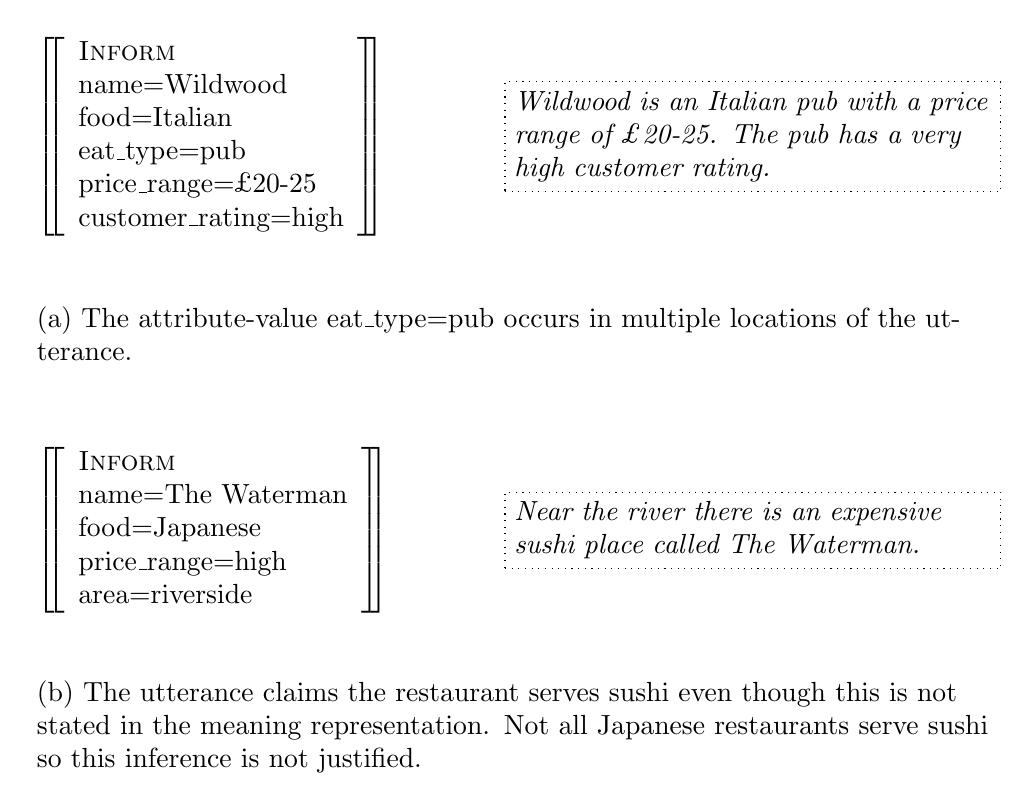
\begin{tikzpicture}

    \node[align=left,text width=\textwidth] (a) at (0,0) 
    {(a) The \attributevalue~eat\_type=pub occurs in multiple locations 
    of the utterance.};

    \node[anchor=west] at ($(a.west)+(0,2.5)$) {
        $\left[\!\!\left[\begin{array}{l}
                    \textsc{Inform}\\
            \AV{name}{Wildwood}\\
            \AV{food}{Italian}\\
            \textrm{eat\_type=}\redbox{\textrm{pub}}\\
            \AV{price\_range}{£20-25}\\
            \AV{customer\_rating}{high}
        \end{array}\right]\!\!\right]$};

    \node[draw,dotted,text width=0.5\textwidth,align=left,anchor=east] 
        at ($(a.east)+(0,2.5)$) 
        {\textit{Wildwood is an Italian \redbox{pub} with a price range of
        £20-25. The \redbox{pub} has a very high customer rating.}};

%    \node[align=left,text width=\textwidth] (b) at (0,-6) 
%    {(b) The utterance fails to mention the customer rating or that the 
%    establishment is family friendly.};
%
%    \node[anchor=west] at ($(b.west)+(0,3)$) {
%        $\left[\!\!\left[\begin{array}{l}
%                    \textsc{Inform}\\
%            \AV{name}{Blue Spice}\\
%            \AV{eat\_type}{coffee shop}\\
%            \AV{price\_range}{cheap}\\
%            \AV{customer\_rating}{average}\\
%            \AV{area}{riverside}\\
%            \AV{family\_friendly}{yes}\\
%            \AV{near}{Avalon}
%        \end{array}\right]\!\!\right]$};
%
%    \node[draw,dotted,text width=0.5\textwidth,align=left,anchor=east] 
%        at ($(b.east)+(0,3)$) 
%        {\textit{Blue Spice is a cheap coffee shop located  
%         in the riverside, near Avalon.}};


    \node[align=left,text width=\textwidth] (b) at (0,-5) 
    {(b) The utterance claims the restaurant serves sushi even though this
         is not stated in the \meaningrepresentation. Not all Japanese 
         restaurants serve sushi so this inference is not justified.};

    \node[anchor=west] at ($(b.west)+(0,2.5)$) {
        $\left[\!\!\left[\begin{array}{l}
          \textsc{Inform} \\
          \AV{name}{The Waterman}\\ 
          \textrm{food=}\redbox{\textrm{Japanese}}\\ 
          \AV{price\_range}{high}\\
    %      \AV{customer\_rating}{3 out of 5}\\
          \AV{area}{riverside}%\\
  %        \AV{family\_friendly}{yes}
  \end{array}\right]\!\!\right]$};

    \node[draw,dotted,text width=0.5\textwidth,align=left,anchor=east] 
        at ($(b.east)+(0,2.5)$) 
          {\textit{Near the river there is an expensive \redbox{sushi} 
          place called The Waterman.}}; %It is family friendly and rated 3 
           %out of 5.}};

%

%
%%name[Blue Spice], eatType[coffee shop], priceRange[cheap], customer rating[average], area[riverside], familyFriendly[yes], near[Avalon]"
%
%
%
%
%
%%
%%
%%
%%
%%
%%
%
%
%
%

\end{tikzpicture}

\caption{Example training set errors.}
\label{fig:nlgerrors}
\end{figure}


While such examples may exist in the training data, we consider model
generation of such phenomena to constitute a failure to faithfully generate an
utterance.  In the overwhelming majority of cases, each \attributevalue~is
explicitly and uniquely grounded in the target utterances, this makes
\surfacerealization~from \meaningrepresentations~a useful task to study
faithful generation. The baseline task of correctly generating all
\attributevalues~appropriately for the \dialogueact~is hard enough, and it in
this setting we do not have to worry about ungrounded information or
information that is not explicitly represented in the
\meaningrepresentations~but is deducible from the
\meaningrepresentation~\citep{wiseman2017}.  

\section{Modeling \MeaningRepresentation-to-Text Generation with \SequencetoSequence~Architectures}
\label{mrtproblemdef}

\subsection{\SequencetoSequence~Modeling}

We approach the problem of mapping a \meaningrepresentation~to a natural
language utterance with a variety of popular \sequencetosequence~architectures.
A \sequencetosequence~model is a neural network with parameters $\params$ that
implements a probabilistic mapping, $\gen(\cdot|\cdot;\params) : \inSpace
\times \outSpace \rightarrow (0,1)$, from input sequences 
\[
    \mrtoks = \left[\mrtok_1,\ldots,\mrtok_\mrSize\right] \in \inSpace
\]
to output sequences 
\[
    \utttoks = \left[\utttok_1, \ldots, \utttok_\uttSize\right] \in \outSpace.
\]
Tokens from the input sequence are drawn from a finite vocabulary $\mrvocab$
and input sequences its Kleene closure $\mrvocab^* = \inSpace$.  Analogously,
tokens from the output sequence are drawn from a distinct, finite vocabulary
$\uttvocab$ and output sequences its Kleene closure $\uttvocab^* = \outSpace$.
For clarity we occasionally omit $\params$ in subsequent equations.

Typically, \gen~is implemented as a bipartite network consisting of distinct
encoder and decoder networks $\encMod$~and \decMod~respectively.  The encoder
$\encMod : \inSpace \rightarrow \reals^{*\times\encDim}$ is a mapping of an
input sequence $\mrtoks$ of $\mrSize$ tokens to $\mrSize$ corresponding vectors
$\encState_1,\ldots\encState_\mrSize \in \reals^\encDim$ and
\[ 
    \gen(\utttoks|\mrtoks) = \gen(\utttoks|\encMod(\mrtoks)) = \gen(\utttoks|\encState_1,\ldots,\encState_\mrSize).
\]
The decoder $\decMod : \uttvocab^+ \times \reals^{*\times \encDim} \rightarrow
(0,1)$ then is a mapping of previously generated tokens $\utttoks_{1:i-1} =
\left[\utttok_1,\ldots,\utttok_{i-1}\right]$ and encoder states
$\encState_1,\ldots,\encState_\mrSize$ to a probability distribution over the
output vocabulary $\uttvocab$, where
\[ 
    \gen(\utttok_i|\utttoks_{1:i-1},\mrtoks) = \decMod\left(\utttoks_{1:i}, \encMod(\mrtoks)\right)   \quad \textrm{and} \quad \sum_{\utttok\in \uttvocab} \gen\left(\utttok| \utttoks_{1:i-1}, \encMod(\mrtoks)\right) = 1.  
\]
Hence, $\gen(\cdot|\mrtoks)$ is a conditional language model over utterance
tokens that factorizes in a left-to-right fashion, i.e.,
\[
    \gen\left( \utttoks| \mrtoks \right) = \prod_{i=1}^\uttSize \gen\left(\utttok_i|\utttoks_{1:i-1},\mrtoks\right). 
\]

Notice that the ``inputs'' and ``outputs'' to the \sequencetosequence~model are
sequences of tokens, $\mrtoks$ and $\utttoks$ respectively.  In order to use a
\sequencetosequence~model for \naturallanguagegeneration~from a
\meaningrepresentation~we need only map our desired inputs and outputs to
sequences of discrete tokens. In English, the desired output is relatively
straightforward to represent as a sequence as an English language utterance can
naturally be represented as a sequence of word tokens. In practice, we also
indicate full sentence stops with a special token \senttok\footnote{We add an
explicit sentence stop symbol because occasionally utterances have non-sentence
final periods and we want there to be no ambiguity about sentence stops
produced by the model.} and prepend and append distinguished tokens
\starttok~and \stoptok, respectively, to indicate the start and end of the
utterance, as well as lower-case all tokens.  As an example, the utterance 
\[
    \textit{The Vaults pub is near Caf{\'e} Adriatic. It is not a good place for families.} 
\]
would be represented as 
\[\small \utttoks = \left[\starttok, \textit{the},\,\textit{vaults},\,\textit{pub},\,\textit{is},\,\textit{near},\,\textit{caf{\'e}},\,\textit{adriatic},\,\textit{.},\,\textit{\senttok},\,\textit{it},\,\textit{is},\,\textit{not},\,\textit{a},\,\textit{good},\,\textit{place},\,\textit{for},\,\textit{families},\,\textit{.},\,\textit{\stoptok}\right]. \]

The \meaningrepresentation~is not itself a sequence, however, so we cannot
apply it to a \sequencetosequence~model directly.  Instead it must first be
``linearized,'' or mapped to a linear sequence of tokens. We refer to a
function $\ls : \mrspace \rightarrow \inSpace$, as a \linearizationstrategy.
We experiment with several \linearizationstrategies~in this chapter, however,
all of them operate over the same domain, $\mrvocab^+$, where $\mrvocab$
consists of distinct tokens for each \dialogueact~and \attributevalue~pairs.
As an example consider the following \meaningrepresentation,
\begin{singlespace}
  \[ 
    \mr = \left[\!\!\left[\begin{array}{l} \textsc{Inform} \\ \AV{name}{Aromi}\\\AV{area}{city centre} \\ \AV{eat\_type}{coffee shop} \end{array}\right]\!\!\right] \]
\end{singlespace}
\noindent and some possible linearizations,
\begin{align*}
     \ls_1(\mr) & = \mrtoks= \left[\textit{inform},\,\textit{name=Aromi},\,\textit{eat\_type=coffee shop},\,\textit{area=city centre}\right] \\
     \ls_2(\mr) & = \mrtoks= \left[\textit{inform},\,\textit{eat\_type=coffee shop},\,\textit{name=Aromi},\,\textit{area=city centre}\right] \\
     \ls_3(\mr) & = \mrtoks= \left[\textit{inform},\,\textit{eat\_type=coffee shop},\,\textit{area=city centre},\,\textit{name=Aromi}\right].
\end{align*}
In practice, regardless of the choice of \linearizationstrategy, we prepend a
start token, $\starttok$, and append and a stop token, $\stoptok$, to all
input token sequences, e.g.
\[ \mrtoks = \left[\starttok,\,\textit{inform},\,\textit{name=Aromi},\,\textit{eat\_type=coffee shop},\,\textit{area=city centre},\,\stoptok\right]. \]

The encoder and decoder networks of the \sequencetosequence~model can be
implemented with a variety of architectures. We use two such architectures, the
gated recurrent unit (GRU) \citep{cho2014learning} and the transformer
\citep{vaswani2017}. Since we use standard variants, we defer explicit model
definitions to \hyperref[sec:nlggru]{Appendix \ref{sec:nlggru}} and
\hyperref[sec:nlgtf]{Appendix \ref{sec:nlgtf}} for GRU- and transformer-based
sequence-to-sequence architectures respectively. While the GRU must be given an
explicit linearization to process any input, the transformer variant does not
have to be sensitive to linearization order. However, when the transformer uses
position embeddings, which is the standard configuration, it is sensitive to
linearization order. We always use position embeddings in this work as
\cite{vaswani2017} found the model did not work as well without them.

\subsection{Learning}

Given a dataset of \meaningrepresentation/utterance pairs, $\corpus =
\left\{\left(\mr^{(1)}, \utttoks^{(1)}\right), \ldots,
\left(\mr^{(\corpusSize)},\utttoks^{(\corpusSize)} \right)\right\}$, and a
\linearizationstrategy, $\ls$, the parameters, $\params$, of $\gen$~can be
learned by approximately minimizing the negative log-likelihood of the data,
\[ \hat{\params} \approx \argmin_{\params \in \Params} -\frac{1}{\corpusSize}\sum_{\left(\mr, \utttoks \right) \in \corpus} 
    \log \gen\left(\utttoks|\ls\left(\mr\right);\params\right).
\]
In practice, this is done with some variant of mini-batch stochastic gradient
descent, e.g., Adam \citep{kingma2014adam}.  Additionaly, label smoothing
\citep{szegedy2016} and non-linear learning rates are often necessary in
practice for optimizing the transformer-based \sequencetosequence~model.
Dropout is also typically applied to both the GRU and transformer models during
training. 

\begin{algorithm}[t]
\KwData{~\\$\quad\mrtoks:$ input sequence\\$\quad\nbest:$ beam size\\$\quad T:$ maximum utterance length\\ $\quad\gen :$ generation model for scoring candidates.\\
$\quad\operatorname{rerank-score} :$ reranking hypothesis scoring function. }
$\mathcal{H} \gets \left\{\left[\starttok\right]\right\}$\\
$\mathcal{H}_{complete} \gets \left\{ \right\}$\\
\For{$i =1,\ldots, T$}{
    $\mathcal{H}_{new} \gets \left\{ \right\}$ \\
    \For{$\utttoks = \left[\utttok_1,\ldots,\utttok_i \right]\in \mathcal{H}$}{
        \If{$\utttok_i = \stoptok$}{
            $\mathcal{H}_{complete} \gets \mathcal{H}_{complete} \cup \{ \utttoks \}$\\
            $\mathcal{H} \gets \mathcal{H} \setminus \{ \utttoks \}$\\
        }

        \For{$\utttok^\prime \in \uttvocab$}{
            $\mathcal{H}_{new} \gets \mathcal{H}_{new} \cup \left\{\left[ \utttok_1,\ldots,\utttok_i, \utttok^\prime\right] \right\}$
        }
    }
    $\mathcal{H} \gets \operatorname{Top}_\nbest(\mathcal{H}_{new}, \gen(\cdot|\mrtoks))$\\

}

\KwResult{$\operatorname{Top}_1(\mathcal{H}_{complete}, \operatorname{rerank-score}(\cdot|\mrtoks))$}

\caption{Beam Search}
\label{alg:beamsearch}
\end{algorithm}


\subsection{Inference}
\label{sec:nlginference}

As stated above, $\gen\left(\cdot|\ls\left(\mr\right)\right)$ is a conditional
language model.  Given some \meaningrepresentation~$\mr$, a natural utterance
one might want to infer is the maximum a posteriori (MAP) utterance 
\[
 \predutttoks = \argmax_{\utttoks\in\uttSize} \log\gen\left(\utttoks|\ls\left(\mr\right)\right) 
\] 
under the model.\footnote{Technically, we are only considering valid finite
utterances $\utttoks = \left[\utttok_1,\ldots,\utttok_\uttSize\right] \in
\outSpace$ with $\utttok_1 = \starttok$ and $\utttok_\uttSize = \stoptok$. }
Unfortunately, the search implied by the $\argmax$ is intractable. Instead an
approximate search is performed. The most commonly used search is called
\textit{beam search} \citep{reddy1977} or beam decoding.  Under beam search, a
set $\mathcal{H}$ of $\nbest$-best candidate utterances is maintained
throughout the search. $\nbest$ is referred to as the beam size or beam width.
At each step $i$ of the search, the next word continuations are computed for
each candidate utterance prefix, yielding $\nbest \times \lvert\uttvocab\rvert$
utterances, from which the top-$\nbest$ under some search criterion are
selected, and $\mathcal{H}$ is updated the with the $\nbest$ utterances of
length $i+1$.  When a completed utterance enters $\mathcal{H}$ (i.e.,
$\utttok_{i+1} = \stoptok$), it is added to a set of completed utterances,
$\mathcal{H}_{complete}$, and removed from $\mathcal{H}$.  After exploring the
maximum number of steps $T$ (or some other heuristic stopping criterion),
$\mathcal{H}_{complete}$ is reranked according some heuristic reranking
criteria, and the top-ranked  utterance is returned.  When the beam size is 1,
we refer to the algorithm as greedy search or greedy decoding.  See
\autoref{alg:beamsearch} for a formal description of the algorithm.

Common reranking criteria include the length-normalized log likelihood, \[
\operatorname{rerank-score}(\utttoks,\mr) = \frac{\sum_{i=1}^\setsize{\utttoks}
\log \gen(\utttok_i|\utttoks_{1:i-1},\ls(\mr))}{\setsize{\utttoks}}\] or a
mixture of model likelihood and an auxiliary  language model, $\gen_{LM}$, \[
\operatorname{rerank-score}(\utttoks,\mr) = \log\gen(\utttoks|\ls(\mr)) +
\lambda \log \gen_{LM}(\utttoks).\] The latter method is popular in machine
translation where it is easier to obtain a large monolingual corpus with which
to train a language model than it is to obtain a large parallel corpus for
training the translation model \citep{xie2017neural}. When using
\sequencetosequence~models for the \meaningrepresentation-to-text generation
problem, practitioners often incorporate a discriminative
\meaningrepresentation~parser, $\dmodel(\cdot|\cdot) : \mrspace \times
\outSpace \rightarrow (0,1)$, in the reranker, \[
\operatorname{rerank-score}(\utttoks,\mr) = \log\dmodel(\mr|\utttoks),\] which
can help to select the most semantically correct utterances from the beam
candidates. Under this setting, for a candidate utterance $\predutttoks \in
\mathcal{H}_\textrm{complete}$ obtained with $ \gen\left( \cdot | \ls (\mr)
\right)$ using beam search, $\dmodel\left( \mr | \predutttoks \right)$ gives
the probability that $\denotes{\predutttoks} = \mr$ under the model $\dmodel$.

Despite its wide adoption and empirical success, however, there are many known
issues with beam search.  The output may repeat phrases or words
\citep{holtzman2019}, or may never even terminate
\citep{welleck2020consistency}.  While these issues are often linked to
differences in the maximum likelihood learning objective and test-time search
procedure \citep{lafferty2001,andor2016}, the problems are possibly deeper as
increasing the beam size often leads to worse empirical performance
\citep{koehn2017}. In fact, the biases present in beam search are actually
beneficial when compared to exact search \citep{stahlberg2019}.  Additionally,
it is well known that the set of output beam candidates may lack diversity and
only differ by a small number of words
\citep{sordoni2015,galley2015,li2016,vinyals2015,serban2016}.

\subsection{Sampling}

As an alternative to deterministic decoding, one may sample from the
conditional distribution, $\gen\left(\cdot|\ls(\mr)\right)$. The typical method
for doing this is called \ancestralsampling. \Ancestralsampling~is very similar
to greedy decoding, and works by sequentially sampling the next word
$\utttok_{i+1} \sim \gen\left(\cdot|\utttoks_{1:i},\ls(\mr)\right)$, and
terminating when $\utttok_{i+1} = \stoptok$. There are several modifications
one might make to \ancestralsampling~in practice. To encourage more diversity
in the sampled outputs, a temperature parameter $\temperature$ is sometimes
added to the final $\softmax$ layer, \[ \gen\left(\utttok_{i+1}|
\utttoks_{1:i},\ls(\mr); \temperature) \right) = \softmax\left(
\frac{\weight{o}\tfDecInputRow_i + \bias{o}}{\temperature}
\right)_{\utttok_{i+1}}.\] As $\temperature$ tends toward $+\infty$, the
conditional distribution becomes less peaked and the differences in probability
between any two words diminish, making it easier to sample an unusual
continuation of the utterance sequence.  In the positive limit, each word
becomes equally likely, \[ \lim_{\temperature\rightarrow +\infty}
\gen\left(\utttok| \utttoks_{1:i},\ls(\mr); \temperature) \right) =
\frac{1}{\setsize{\uttvocab}}.\] As $\temperature$ approaches zero, the
distribution becomes a ``one-hot'' distribution, \[
\lim_{\temperature\rightarrow +0} \gen\left(\utttok| \utttoks_{1:i},\ls(\mr);
\temperature) \right) = \mathds{1}\{\utttok = \argmax_{\utttok^\prime}
\gen\left(\utttok^\prime| \utttoks_{1:i},\ls(\mr)\right)  \}\] where the
probability is zero for every word except the most likely next word in the
original distribution, which now has probability one.

While ancestral sampling can lead to more diverse outputs, the next word
distributions are often quite peaked meaning most of the vocabulary accounts
for less than 0.05 of the cumulative distribution function. For a 20 word
sentence, this means that on average at least one word will be sampled from the
long-tail, effectively choosing a word uniformly at random from the vocabulary.
To avoid this issue, two heuristic modifications are often made to ancestral
sampling, \textit{top-$k$} sampling \citep{fan2018,holtzman2018,radford2019}
and \textit{nucleus} sampling \citep{holtzman2019}. 

In top-$k$ sampling, $p(\utttok|\utttoks_{1:i},\ls(\mr))$ is restricted to the
top $k$ most likely words. Let $\topkVocab{i}{k} \subset \uttvocab$ be the set
of $k$ most likely next words at sampling step $i$, i.e.,
\[\topkVocab{i}{k} = \argmax_{S \subset \uttvocab, \setsize{S} = k} \sum_{\utttok \in S} \log\gen(\utttok|\utttoks_{1:i},\ls(\mr)). \]
The next word $\utttok_{i+1}$ is then sampled from the following distribution,
\[
    \gen\left(\utttok_{i+1}|\utttoks_{1:i},\ls(\mr);\topkVocab{i}{k}\right)
    =
    \begin{cases} 
   \frac{
   \gen(\utttok_{i+1}|\utttoks_{1:i},\ls(\mr))
   }{ 
       \sum_{\utttok^\prime \in \topkVocab{i}{k}  }
   \gen(\utttok^\prime|\utttoks_{1:i},\ls(\mr))  
   }  & \utttok_{i+1} \in \topkVocab{i}{k} \\ 
0 & \textrm{otherwise}. \end{cases} 
\]

\citet{holtzman2019} show that picking the right $k$ for top-$k$ sampling is
difficult because the next word distribution can alternate from very flat
(which would suggest a large $k$) to very peaked (which would suggest a small
$k$).  Instead they propose restricting the subset of vocabulary to sample from
to the smallest set of words such that their cumulative probability is greater
than a threshold $\nucleusthr$,
\[ \nucleusVocab{i}{\nucleusthr} = \argmin_{\substack{S \subset \uttvocab \\
\sum_{\utttok \in S} \gen(\utttok|\utttoks_{1:i},\ls(\mr)) \ge \nucleusthr  }}
\setsize{S}. \] The sampling distribution for this method which they call
nucleus sampling, is computed similarly to top-$k$ sampling,
\[
\gen\left(\utttok_{i+1}|\utttoks_{1:i},\ls(\mr); \nucleusVocab{i}{\nucleusthr} \right)
    =
    \begin{cases} 
   \frac{
   \gen(\utttok_{i+1}|\utttoks_{1:i},\ls(\mr))
   }{ 
       \sum_{\utttok^\prime \in \nucleusVocab{i}{\nucleusthr} }
   \gen(\utttok^\prime|\utttoks_{1:i},\ls(\mr))  
   }  & \utttok_{i+1} \in \nucleusVocab{i}{\nucleusthr} \\ 
0 & \textrm{otherwise}. \end{cases} 
\]
Nucleus sampling helps avoid sampling from the long tail of the distribution
while still producing diverse samples.

\section{Faithful Generation Through Data-Augmentation: Noise-Injection Sampling and Self-Training}
\label{sec:nlgfg}

We now formally define faithfulness as it relates to the
\meaningrepresentation~to text generation problem.  Let $\GEN : \mrspace
\rightarrow \outSpace$ be an arbitrary mapping from \meaningrepresentations~to
utterances. We say that a mapping $\GEN$ is \faithful~if \[\denotes{\GEN(\mr)}
= \mr \quad \forall \mr: \mr \in \mrspace.\] In words, $\GEN$ is faithful if
the propositional content of $\mr$ (i.e., the semantics of the
\attributevalue~pairs in $\mr$) is correctly expressed by the generated
utterance $\predutttoks = \GEN(\mr)$ for any well-formed
\meaningrepresentation~$\mr$. 

If $\GEN$ is implemented with templates as in \cite{puzikov2018}, it is
possible to design a faithful mapping. However, it is possible that
faithfulness and naturalness are in tension, as the method of
\cite{puzikov2018} did not perform as highly on human judgements of
naturalness.

It is well known that implementing $\GEN$ with a neural model $\gen$ and an
inference procedure such as beam search are not sufficient to obtain a faithful
model.  Beam search, which only expands candidates whose next word
continuations are highly probable, tends to produce low-perplexity utterances
\citep{serban2016}. Low-perplexity utterances may satisfy perceived notions of
quality \citep{meister2020}, but this is not a sufficient condition for
semantic correctness.  As mentioned in \autoref{sec:nlginference},  a common
approach to make $\gen$ more faithful is to perform overgeneration with
reranking \citep{dusek2016,juraska2018,dusek2019,dusek2020}.  The $\nbest$-best
list of utterances $\mathcal{H}_{complete} = \left\{\utttoks^{(1)},\ldots,
\utttoks^{(\nbest)}\right\}$ is produced using beam search with
$\gen\left(\cdot|\ls(\mr)\right).$ Then a discriminative
\meaningrepresentation~parser, $\dmodel(\cdot|\cdot) : \mrspace \times
\outSpace \rightarrow (0,1)$, is used to rerank $\mathcal{H}_{complete}$ such
that the final output utterance is \[ \predutttoks = \argmax_{\utttoks \in
\mathcal{H}_{complete}} \dmodel\left(\mr\vert\utttoks\right). \] In this
setting the inference procedure selects the utterance that most likely denotes
the input $\mr$ under $\dmodel$. While this reduces the risk of generating an
incorrect utterance with respect to $\mr$, it can still fail when either
$\dmodel$ is not accurate or when $\mathcal{H}_{complete}$ does not contain a
completely correct utterance.

The critical issue here is that the final beam search hypothesis set may not
contain any completely semantically correct utterances.  This in part happens
because neural models on natural language data\footnote{Here we are referring
to both \sequencetosequence~models but also sequence classification
\citep{kim2014convolutional,mccoy2019} and sequence-pair classification
\citep{he2019}. }  do not na{\"i}vely exhibit the quality of systematicity
\citep{fodor1988,phillips1998,marcus2003,lake18,mccoy2019,gardner2020}. A model
displays systematicity if the capability of the model to  perform a task
implies that it can perform other structurally related tasks successfully.  On
natural language data, a model with systematicity should be able to exploit the
algebraic and compositional nature of natural language to make correct
inferences. \citet{lake18} give the example of a human speaker that understands
the concept of ``twice'' or ``again,'' who, upon learning a novel verb, ``to
dax,'' immediately understands the meaning of ``daxed twice'' or ``to dax
again'' even though they have never seen examples of these compositions before.
Empirically, they demonstrate that a \recurrentneuralnetwork~based
text-to-\meaningrepresentation~model  does not possess this ability and
frequently fails to generalize to novel compositions even where the individual
constituents of the compositions are well represented in the training data.
\cite{bastings2018} show that this also holds going the other direction, from
\meaningrepresentation~to text, the more relevant direction for our present
discussion.

In our case, this lack of systematicity manifests itself as a failure to
realize individual \attributevalues~that are well represented in the training
data when those \attributevalues~occur in novel combinations in a
\meaningrepresentation~at test time. We use as a case-study, the
\attributevalue~\textit{near=Burger King}. which in our restaurant domain
dataset, the E2E Challenge dataset \citep{dusek2018}, denotes that a restaurant
$x$ is near Burger King. 

The \attributevalue~\textit{near=Burger King} appears frequently in the
training data in longer \meaningrepresentation/utterance pairs. In fact
\textit{near=Burger King} is positively associated with
\meaningrepresentations~where seven or eight \attributes~are specified (there
are eight total unique attributes on this dataset). See \autoref{fig:bkpmi}
where we plot the point-wise mutual information (PMI) \citep{church1990} of the
occurrence of the \textit{near=Burger King} and the occurrence of a
\meaningrepresentation~of a particular size on the training set, where the size
of a \meaningrepresentation~$\setsize{\mr}$ is the number of
\attributevalue~pairs in $\mr$.  The PMI is computed as 
\[\pmi(\AV{near}{Burger King},  \setsize{\mr} = k) = \log \frac{p(\AV{near}{Burger King}, \setsize{\mr} = k)}{p( \AV{near}{Burger King}  ) p(\setsize{\mr} = k)}     \quad \forall k : k \in \{3,\ldots,8\},\]
with \begin{align*}
    p(\AV{near}{Burger King}) &= \frac{\sum_{(\mr,\utttoks) \in \corpus}\mathds{1}\left\{ \AV{near}{Burger King} \in \mr \right\}}{\setsize{\corpus}} \\
    p(\setsize{\mr}=k) &= \frac{\sum_{(\mr,\utttoks) \in \corpus}\mathds{1}\left\{ \setsize{\mr} = k \right\}}{\setsize{\corpus}} \\
    p(\AV{near}{Burger King},\setsize{\mr}=k) &= \frac{\sum_{(\mr,\utttoks) \in \corpus}\mathds{1}\left\{\AV{near}{Burger King} \in \mr \wedge \setsize{\mr} = k \right\}}{\setsize{\corpus}}.
\end{align*}
From \autoref{fig:bkpmi} we can see that \textit{near=Burger King}~is
negatively associated with smaller \meaningrepresentations, suggesting a neural
model will struggle to generate utterances for it in the smaller
\meaningrepresentation~regime.

\begin{figure}[t]
\centering
    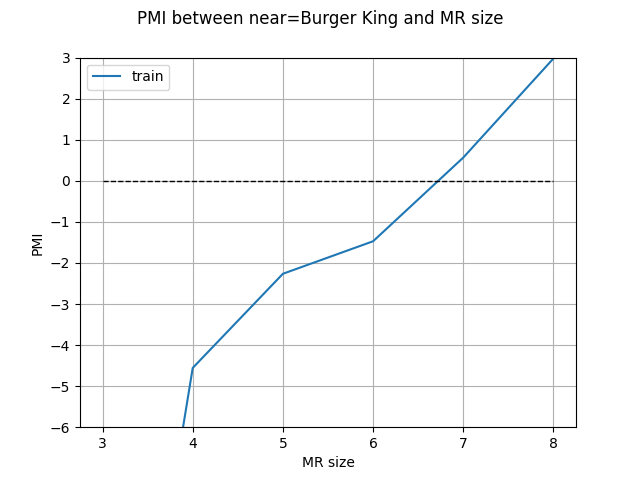
\includegraphics[scale=0.5]{nlg/nearbk.png}
\caption{PMI between \AV{near}{Burger King}~and \meaningrepresentation~size
on the E2E Challenge dataset. 0 on the $y$-axis indicates the two variables are independent.}
\label{fig:bkpmi}
\end{figure}


To demonstrate this, we trained a uni-directional GRU generation model on the
training corpus and then tried to generate an utterance for the following
\meaningrepresentation,
\begin{singlespace}
\[\mr = \left[\!\!\left[\begin{array}{l}\textsc{Inform}\\
        {\AV{name}{Alimentum}}  \\
        {\AV{near}{Burger King}}\\
        {\AV{area}{city centre}}\\
        {\AV{family\_friendly}{no}}\end{array}  \right]\!\!\right],\]
\end{singlespace}
\noindent using beam search. Notice that in this case $\setsize{\mr}=4$,
indicating that the occurrence of \textit{near=Burger King} is a relatively
novel situation given the training set.  We generated some beam search
candidates we show below, {\color{red}\uline{underlining in red}} the phrases
that are not semantically correct given the \meaningrepresentation,

\begin{enumerate}
    \item Alimentum is located in the city centre {\color{red}\uline{near the Express by Holiday Inn.}} It is not family-friendly.     
    \item Alimentum is located in the city centre {\color{red}\uline{near the Yippee Noodle Bar.}} It is not family-friendly.
    \item Alimentum is located in the city centre {\color{red}\uline{near the Raja Indian Cuisine.}} It is not family-friendly.
    \item Alimentum is not family-friendly. It is located in the city centre {\color{red}\uline{near the Yippee Noodle Bar.}}
    \item The Alimentum is located in the city centre {\color{red}\uline{near the Express by Holiday Inn.}} It is not family-friendly.
        %Alimentum is not family-friendly. It is located in the city centre near the Raja Indian Cuisine.\\\vspace{-1em}\\
        %Alimentum is located in the city centre near the Clare Hall. It is not family-friendly.\\\vspace{-1em}\\
        %Alimentum is located in the city centre near the crowne plaza hotel. It is not family-friendly.\\\vspace{-1em}\\
        %Alimentum is not family-friendly. It is located in the city centre near the express by holiday inn.\\\vspace{-1em}\\
        %The Alimentum is located in the city centre near the Yippee Noodle Bar. It is not family-friendly.\\\vspace{-1em}\\
        %Alimentum is not family-friendly. It is located in the city centre near the Clare Hall.\\\vspace{-1em}\\
        %The Alimentum is located in the city centre near the Raja Indian Cuisine. It is not family-friendly.\\\vspace{-1em}\\
        %In the city centre near the express by holiday inn is Alimentum. It is not family-friendly.\\\vspace{-1em}\\
        %Alimentum is located in the city centre near the city centre. It is not family-friendly.\\\vspace{-1em}\\
        %Alimentum is located in the city centre near the rice boat. It is not family-friendly.\\\vspace{-1em}\\
        %The Alimentum is not family-friendly. It is located in the city centre near the Yippee Noodle Bar.\\\vspace{-1em}\\
        %Alimentum is located in the city centre near the rainbow vegetarian café. It is not family-friendly.\\\vspace{-1em}\\
        %In the city centre near the Yippee Noodle Bar is the Alimentum. It is not family-friendly.\\\vspace{-1em}\\
        %In the city centre near the Yippee Noodle Bar is Alimentum. It is not family-friendly.\\\vspace{-1em}\\
        %
\end{enumerate}
Right away we are confronted by their homogeneity; utterances 1,2,3 and 5 have
the same syntactic structure, varying only in the phrase ``near X.'' Utterances
1 and 5 differ only by a single word (the initial article \textit{The} in 5).
Most importantly, none of them correctly specify that the Alimentum is near
Burger King. Even with a beam size of 128, the name ``Burger King'' is never
generated by the model!\footnote{A beam size of 128 would be impractical for
most applications. Beam sizes are typically from 4-10 in most works.}


\begin{figure}[p]
\centering
    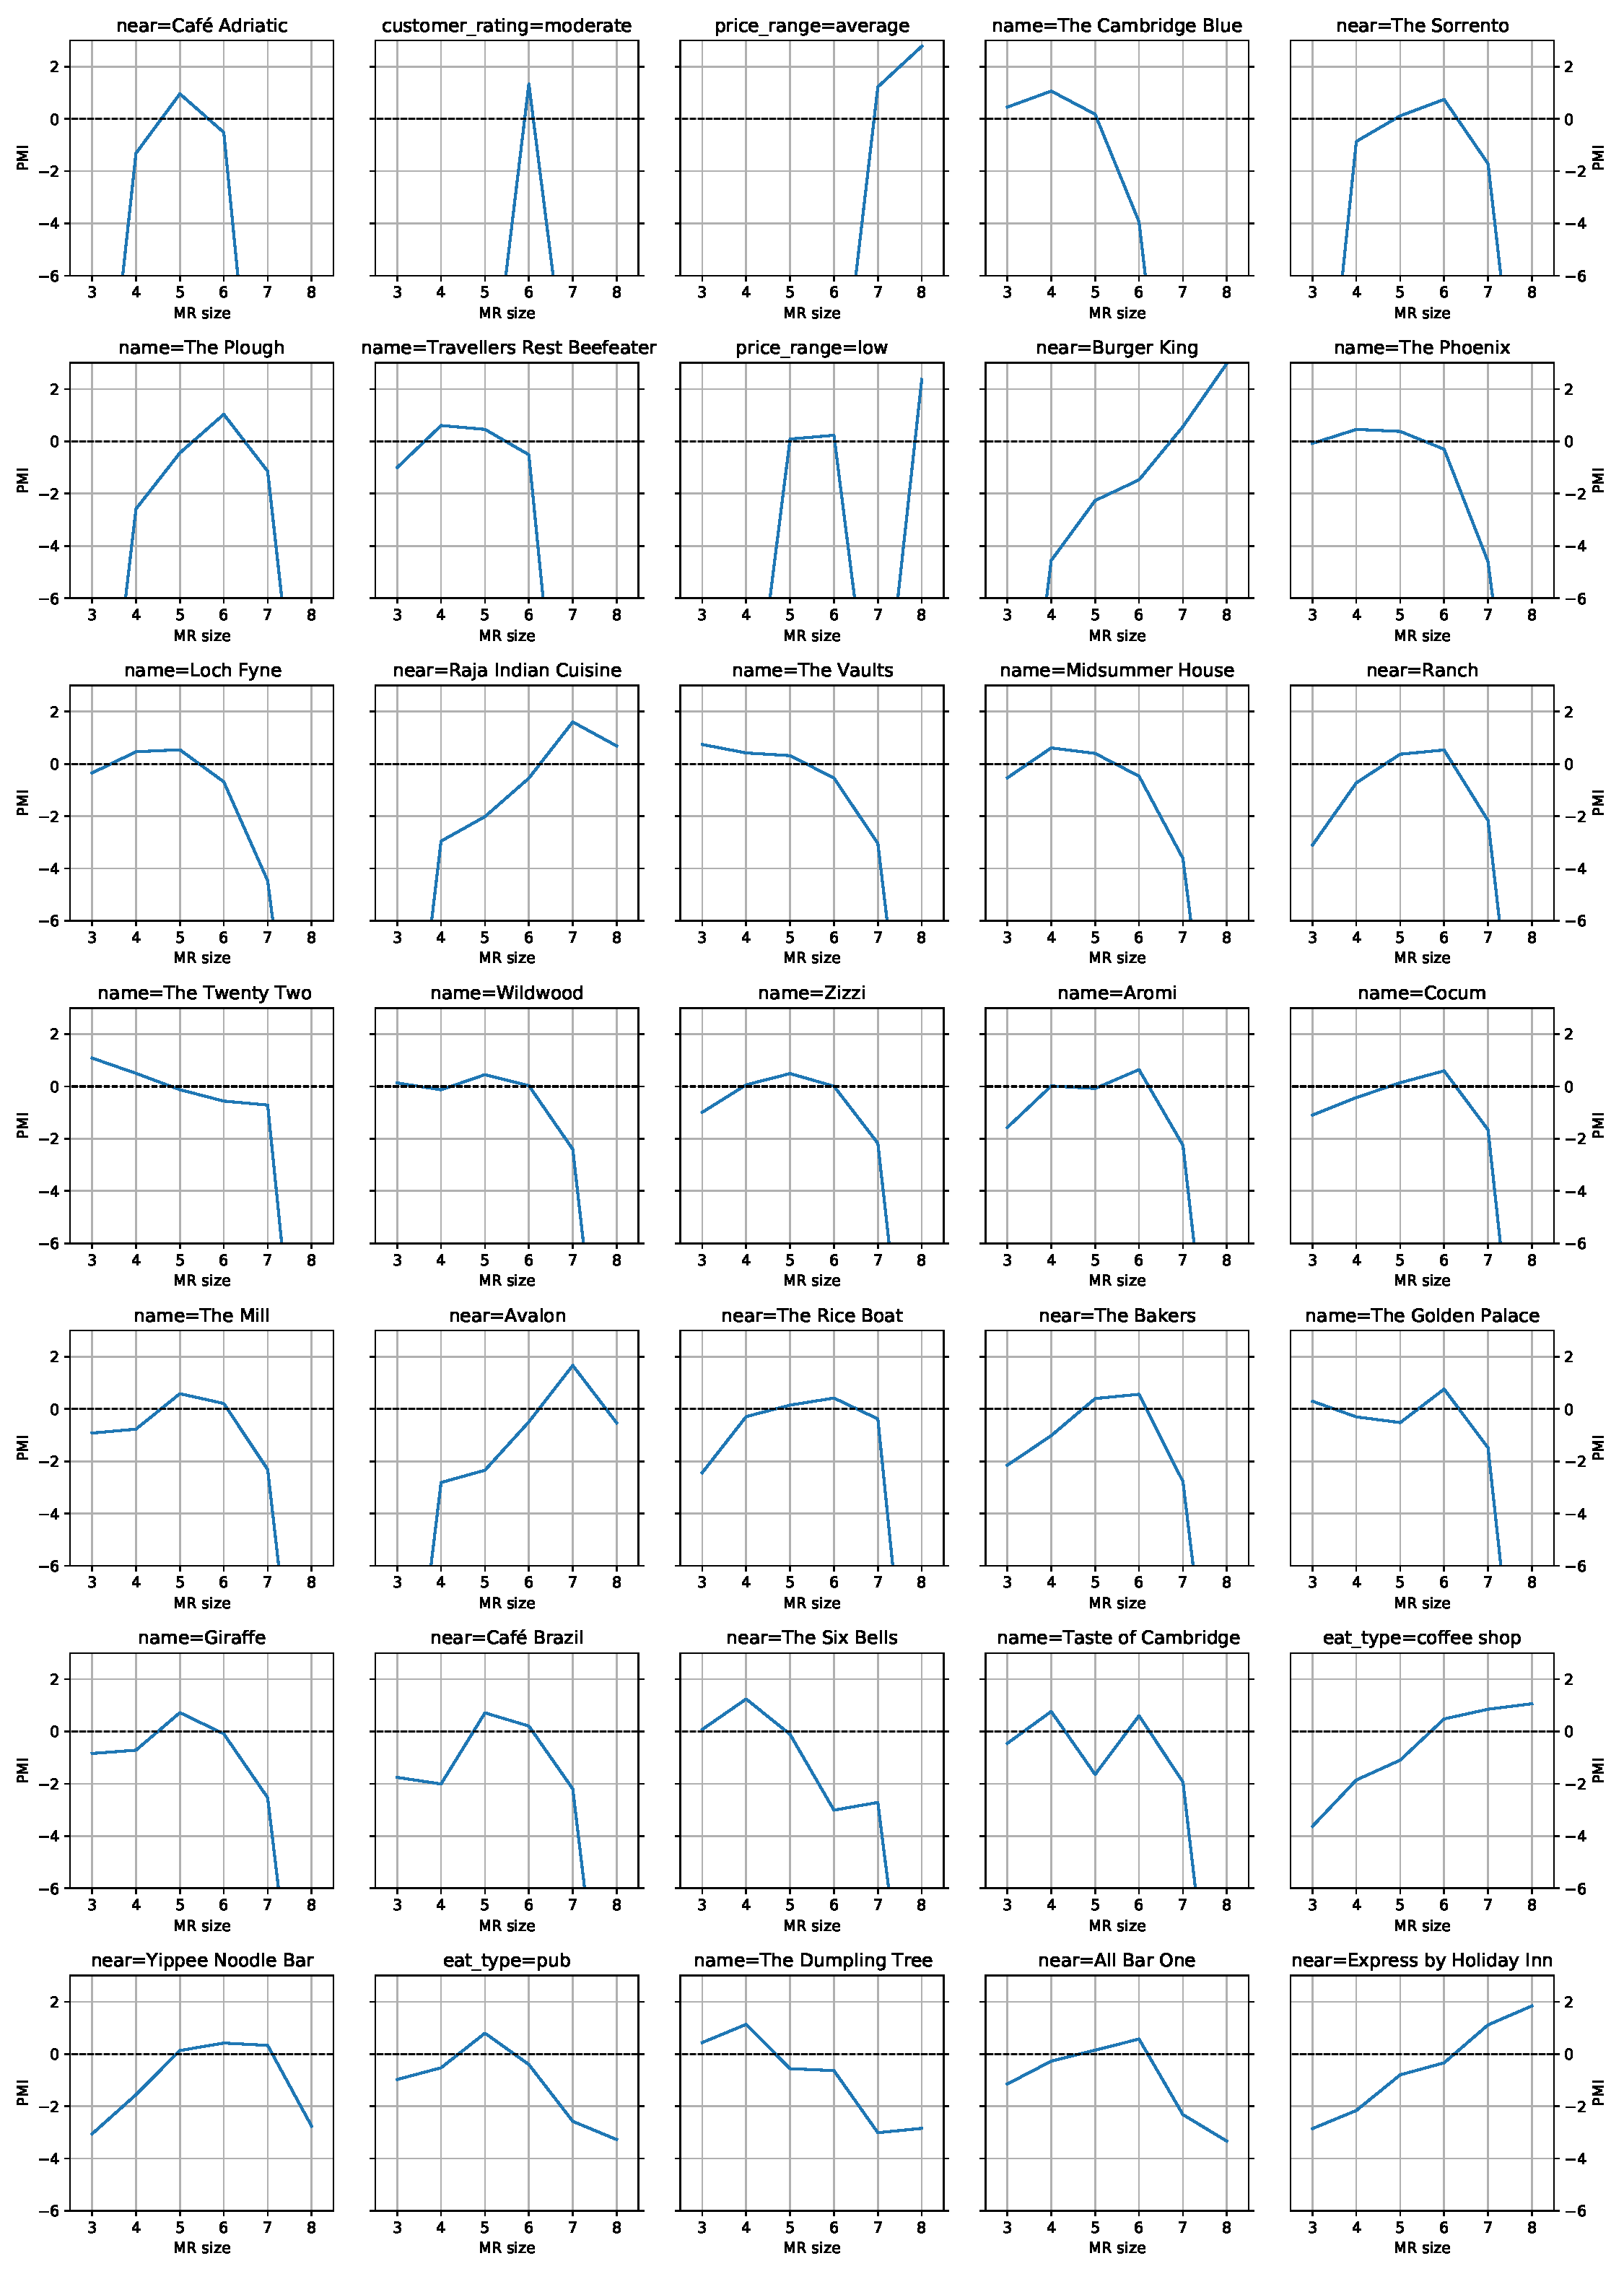
\includegraphics[width=0.9\textwidth]{nlg/trainpmis.pdf}
\caption{PMI between various \attributevalue s and \meaningrepresentation~size
on the E2E Challenge dataset. 0 on the $y$-axis indicates the two variables are independent.}
\label{fig:trainpmi}
\end{figure}


This is more frustrating because there are plenty of training examples where
even a coarse understanding of phrase structure would allow construction of a
correct utterance for this case.  For instance, we observe utterances
containing ``near Burger King'' like this,
\begin{quotation}
    \noindent \textit{The Eagle is a low rated coffee shop \textbf{near Burger King}
        and the riverside that is family friendly and is less than £20
    for Japanese food.}
\end{quotation}
while also seeing
\begin{quotation}
    \noindent \textit{Alimentum is located in the city centre \textbf{near Yippee Noodle Bar}. \textellipsis}
    % It serves expensive Italian food. It has an average customer rating.
\end{quotation}
where a correct utterance could be created by substituting ``Burger King''
in the latter instance, e.g., 
\begin{quotation}
    \noindent \textit{Alimentum is located in the city centre \textbf{near Burger King}.}
    % It serves expensive Italian food. It has an average customer rating.
\end{quotation}

Unfortunately, the GRU model does not learn to substitute the correct
prepositional phrase. Given that correct examples seem constructable from
constituent phrases, it suggests that a data-augmentation approach might help
to generate additional training examples that do not possess some of the
spurious correlations between \attributevalue s and input size.

Indeed, the compositional data-augmentation scheme proposed by
\citet{andreas2020} demonstrates  improved model systematicity.  Unfortunately,
a rule based system of recombination risks creating disfluencies in the
utterances that could potentially reduce the fluency of the learned model.
Additionally, the number of spurious associations in the dataset are numerous;
see \autoref{fig:trainpmi} for 35 of the total 79 \attributevalue~pairs for the
E2E dataset. They all have some spurious association with
\meaningrepresentation~size. And we haven't even explored other associations
that might exist (e.g. between two \attributevalue~pairs\footnote{One might
argue that it is OK for there to be correlations between the attribute-values,
e.g., maybe there are fewer family friendly restaurants in the city centre.
However, we often expect an NLG system to respond systematically -- given an
arbitrary set of attribute-values, the NLG component should realize them all
correctly, and under this constraint it is desirable that any particular
pairing of attribute values is independent in the NLG model.}).  In the
following subsections, we explore what an ideal data-augmentation policy might
look like and then give a practical implementation of it.

\subsection{An Idealized Data-Augmentation Protocol}
\label{sec:ideal}

We now introduce an idealized data-augmentation protocol and discuss some
potential pitfalls and bottlenecks before proposing our implementation of it.
Let $\corpus_\mrspace$ and $\corpus_\outSpace$ be the empirical distributions
(i.e. training dataset distributions) over the \meaningrepresentations~and
utterances respectively. The empirical distributions exhibit various dataset
creation/annotation artifacts. For example, we have that some attributes  are
correlated with length (i.e., $\corpus_\mrspace(a \in \mr, \setsize{\mr} = k)
\ne \corpus_\mrspace(a \in \mr)\corpus_\mrspace(\setsize{\mr} = k)$) or certain
attributes with each other (i.e., $\corpus_\mrspace(a_1, a_2 \in \mr) \ne
\corpus_\mrspace(a_1 \in \mr)\corpus_\mrspace(a_2\in \mr)$).

Ideally, we could construct novel \meaningrepresentation~examples such that
their distributions did not display these correlations. Let us assume we have
such a distribution, $\corpus_\mr^{-1}$, from which we can sample novel
utterances.  Given a sample $\corpus_\mr^{-1}$, we would then need a
conditional distribution $\daUttDist(\samplmr)$ from which to draw the
appropriate companion utterance $\samutttoks$ such that $\denotes{\samutttoks}
= \samplmr$ while the naturalness/grammaticality of $\samutttoks$ was
consistent with the empirical distribution, i.e. $S(\daUttDist) \approx
S(\corpus_\outSpace)$ where $S$ is a projection of utterances into a syntactic
space that is independent of the content.  Having these two distributions, we
could follow the simple data-augmentation protocol in \autoref{alg:idealda} to
obtain a more systematic language generation model $\gen_*$.

Coming up with a \meaningrepresentation~distribution, $\corpus_\mr^{-1}$, is
fairly straightforward.  For example we could just sample the size of the
\meaningrepresentation, $k$, uniformly at random, then sample the $k$
\attributes~uniformly at random without replacement. This would ensure that
attributes and \meaningrepresentation~size are independent and ensure that
\attributes~are not correlated with each other. To make up for the fact that
some \attributevalues~are over-represented in the training set, we could sample
values inversely proportional to their empirical frequency. This results in the
following data generation process for 
\begin{singlespace}\[
        \tilde{\mr}  = \left[\!\!\left[ 
                \begin{array}{c} 
                    \delta~~~~~~~ \\
                    \AV{$a_1$}{$v_1$} \\ \vdots \\ \AV{$a_k$}{$v_k$}  
                \end{array}  
\right]\!\!\right] \sim \corpus_\mr^{-1},\]\end{singlespace}
{
    \begin{minipage}{0.9\textwidth}
        \begin{singlespace}
            \noindent \textit{(1) Draw a dialogue act.}
            \[
                \delta \sim \operatorname{Uniform}(\left\{\delta_1, \delta_2,\ldots\right\}) 
            \]
            \noindent \textit{(2) Draw a \meaningrepresentation~size $k$.}
            \[
                k \sim \operatorname{Uniform}(\{k_{min}, \ldots, k_{max}\}) 
            \]
            \noindent \textit{(3) Sample $k$ attributes without replacement.}
            \[
            a_i  \sim \operatorname{Uniform}(\{name, \ldots, near, eat\_type\}\setminus\{a_1,\ldots,a_{i-1}\}) \quad \forall i: i \in  \{1,\ldots, k\}\]
            \noindent \textit{(4) Sample a value $v_i$ for each attribute $a_i$.}
            \[ v_i  \sim \operatorname{Categorical}\left(\operatorname{count}(v_1)^{-1}, \operatorname{count}(v_2)^{-1},\ldots\right)  \quad \forall i: i \in \{1,\ldots,k\}. \]
        \end{singlespace}
\end{minipage}}

\begin{algorithm}[t]
    $\augdata \gets \{\}$\\
    \While{$\setsize{\augdata} < \numSamples$}{
        $\tilde{\mr} \sim \corpus_\mr^{-1}$ \\
        $\boldsymbol{\tilde{\utttoks}} \sim \daUttDist(\boldsymbol{\tilde{\mr}})$\\
        %\If{ $\lnot \filter(\tilde{\mr}, \boldsymbol{\tilde{\utttoks}})$}{ $\augdata \gets \augdata \cup \{(\tilde{\mr}, \boldsymbol{\tilde{\utttoks}}) \}$ }
        $\augdata \gets \augdata \cup \{(\tilde{\mr}, \boldsymbol{\tilde{\utttoks}}) \}$
    }
    %    \KwResult{Salience judgements $\bsals = \left[ \bsal_1, \ldots, \bsal_\docSize\right]$}
    $\gen_* \gets \operatorname{Train}(\corpus \cup \augdata)$\\
    \KwResult{$\gen_*$}
    \caption{Idealized Data-Augmentation and Training}
    \label{alg:idealda}
\end{algorithm}~\\

Unfortunately, it is not clear how we implement utterance distribution
$\daUttDist(\samplmr)$ since if we had an utterance generation method that
could respond systematically to non-training data distributed
\meaningrepresentations, we wouldn't need to perform data augmentation in the
first place. As a starting point, we consider ways of generating samples from a
base model $\gen_0$  trained on the available training data, i.e.  $\gen_0 =
\operatorname{Train}(\corpus)$.

\subsection{Conditional Utterance Sampling for Data-Augmentation}

We cannot use $\gen_0$ with beam search as we saw previously; there are some
\meaningrepresentations~that $\gen_0$ won't be able to create utterances for
(as we saw with \textit{near=Burger King}). We could try a variant of ancestral
sampling, but it is difficult for ancestral sampling schemes to produce
extremely different outputs that break from spurious associations learned from
the training distribution without hurting fluency. 

The fundamental issue with ancestral sampling is that the randomness of the
model is located at the word selection stage. This means that in the middle of
generating a phrase it is possible for a disfluent word to be selected, which
can disrupt the current phrase but also destabilize subsequent generation steps
as the model tries to recover from the unusual selection.  Ideally, randomness
in a model would occur earlier in determining the ``topicality'' or
``aboutness'' (you might even say content selection) of the generated
utterance. 

Beyond the conditioning input $\ls(\mr)$, the content that is to be generated
is implicitly represented by inner hidden states of the model.  In
\citet{cho2016}, they argue that the hidden states, $\decHidState_i$, of the
\sequencetosequence~decoder lie on a manifold, as a requirement of learning the
next word prediction, i.e.  $\hat{\utttok} = \argmax_\utttok
\gen(\utttok|\utttoks_{1:i},\ls(\mr)) = \argmax_\utttok \left(\weight{o}
\decHidState_i + \bias{o}\right)_\utttok$ implies that $\hat{\utttok}$ must be
linearly separable from other words $\utttok^\prime \in \uttvocab$ along the
hidden state manifold. The implication is that moving about the manifold will
change the ``topicality'' of the distribution
$\gen(\utttok|\utttoks_{1:i},\ls(\mr))$.  They further suggest adding Gaussian
noise to $\decHidState_i$ as a way to obtain random samples from $\gen$, which
we refer to as \textit{noise-injection sampling}.  While \citet{cho2016} used
noise-injection sampling as a means to generate semantically correct but
syntactically diverse outputs, one of our contributions is to use this scheme
as a means to generate semantically divergent outputs (that maintain
grammaticality), for use as a data-augmentation tool.

\newtcbox{\stochbox}[1][]{colframe=blue, colback=blue!15, boxrule=0.1mm,
                       nobeforeafter, tcbox raise base, shrink tight, extrude
                       by=0.32mm, #1}
\newtcbox{\detbox}[1][]{colframe=red, colback=red!15, boxrule=0.1mm,
                       nobeforeafter, tcbox raise base, shrink tight, extrude
                       by=0.32mm, #1}


\renewcommand{\algorithmcfname}{Alg.}

\begin{figure}[t]
\begin{center}\small \detbox{Deterministic operation}~~~~\stochbox{Stochastic operation}\end{center}
\resizebox{\textwidth}{!}{%
\begin{minipage}{0.33\textwidth}
\small
\begin{singlespace}
\begin{algorithm}[H]
$\encHidState_{1:\mrSize} \gets \operatorname{enc}(\ls(\mr))$\\
$\predutttok_1 \gets \starttok$\\
$\predutttoks \gets \left[ \predutttok_1\right]$\\
$i \gets 1$\\
\While{$\predutttok_i \ne \stoptok$}{
$\decHidState_i \gets \operatorname{dec}(\predutttoks, \encHidState_{1:\mrSize})$\\
$\vphantom{\boldsymbol{\epsilon_i} \sim \operatorname{Normal}(\zeroEmb, \frac{\sigma}{i})}$\\
\detbox{$\predutttok_{i+1} \gets \argmax_\utttok \gen(\utttok|\decHidState_i)$}\\
$\predutttoks \gets \predutttoks \oplus \left[ \predutttok_{i+1}\right]$\\
$i \gets i + 1$\\
}
%$\gen_* \gets \operatorname{Train}(\corpus \cup \augdata)$\\
\KwResult{$\predutttoks$}
    \caption{\small Greedy Decoding}
%\label{alg:idealda}
\end{algorithm}
\end{singlespace}
\end{minipage}\begin{minipage}{0.33\textwidth}
\small
\begin{singlespace}
\begin{algorithm}[H]
$\encHidState_{1:\mrSize} \gets \operatorname{enc}(\ls(\mr))$\\
$\predutttok_1 \gets \starttok$\\
$\predutttoks \gets \left[ \predutttok_1\right]$\\
$i \gets 1$\\
\While{$\predutttok_i \ne \stoptok$}{
$\decHidState_i \gets \operatorname{dec}(\predutttoks, \encHidState_{1:\mrSize})$\\
$\vphantom{\boldsymbol{\epsilon_i} \sim \operatorname{Normal}(\zeroEmb, \frac{\sigma}{i})}$\\
\stochbox{$\predutttok_{i+1} \sim \vphantom{\argmax_\utttok}\gen(\cdot|\decHidState_i)$}\\
$\predutttoks \gets \predutttoks \oplus \left[ \predutttok_{i+1}\right]$\\
$i \gets i + 1$\\
}
%$\gen_* \gets \operatorname{Train}(\corpus \cup \augdata)$\\
\KwResult{$\predutttoks$}
\caption{\small Ancestral Sampling}
%\label{alg:idealda}
\end{algorithm}
\end{singlespace}
\end{minipage}\begin{minipage}{0.38\textwidth}
\small
\begin{singlespace}
\begin{algorithm}[H]
$\encHidState_{1:\mrSize} \gets \operatorname{enc}(\ls(\mr))$\\
$\predutttok_1 \gets \starttok$\\
$\predutttoks \gets \left[ \predutttok_1\right]$\\
$i \gets 1$\\
\While{$\predutttok_i \ne \stoptok$}{
$\decHidState_i \gets \operatorname{dec}(\predutttoks, \encHidState_{1:\mrSize})$\\
\stochbox{$\boldsymbol{\epsilon_i} \sim \operatorname{Normal}(\zeroEmb, \frac{\sigma}{i})$}\\
\detbox{$\predutttok_{i+1} \gets \argmax_\utttok \gen(\utttok|\decHidState_i + \boldsymbol{\epsilon_i})$}\\
$\predutttoks \gets \predutttoks \oplus \left[ \predutttok_{i+1}\right]$\\
$i \gets i + 1$\\
}
%$\gen_* \gets \operatorname{Train}(\corpus \cup \augdata)$\\
\KwResult{$\predutttoks$}
\caption{\small Noise Injection Sampling}
%\label{alg:idealda}
\end{algorithm}
\end{singlespace}
\end{minipage}
}
\caption{A comparison of greedy decoding, ancestral sampling, and noise injection sampling.}
\label{fig:noiseinj}

%?\begin{minipage}{0.3\textwidth}
%?\begin{singlespace}
%?\begin{algorithm}[H]
%?$\predutttok_1 \gets \starttok$\\
%?$i \gets 1$\\
%?\While{$\predutttok_i \ne \stoptok$}{
%?$\tilde{\mr} \sim \daMrDist$ \\
%?%\If{ $\lnot \filter(\tilde{\mr}, \boldsymbol{\tilde{\utttoks}})$}{ $\augdata \gets \augdata \cup \{(\tilde{\mr}, \boldsymbol{\tilde{\utttoks}}) \}$ }
%?$\augdata \gets \augdata \cup \{(\tilde{\mr}, \boldsymbol{\tilde{\utttoks}}) \}$
%?}
%?%    \KwResult{Salience judgements $\bsals = \left[ \bsal_1, \ldots, \bsal_\docSize\right]$}
%?$\gen_* \gets \operatorname{Train}(\corpus \cup \augdata)$\\
%?\KwResult{$\gen_*$}
%?    \caption{Noise-Injection Sampling}
%?\label{alg:idealda}
%?\end{algorithm}
%?\end{singlespace}
%?\end{minipage}
\end{figure}




\begin{figure}[t]
\small
\textbf{Ancestral Sampling}\\
\textit{\starttok~the eagle is a non family - friendly italian food establishment . \stoptok}\\
\textit{\starttok~the eagle is a italian food place and is not family - friendly . \stoptok}\\
\textit{\starttok~some italian food can be found at the eagle . \senttok~it 's not family - friendly . \stoptok}\\
\textit{\starttok~the eagle serves italian food . \senttok~it has a \unktok~\unktok~and is not family friendly . \stoptok}\\
\textit{\starttok~the eagle is a family friendly place for italian food . \stoptok}\\
~\\
\textbf{Top-K Sampling ($k=100$)}\\
\textit{\starttok~the eagle serves italian food . \senttok~it is not family - friendly . \stoptok}\\
\textit{\starttok~the eagle serves italian cuisine . \senttok~it is not family - friendly . \stoptok}\\
\textit{\starttok~the eagle has italian food and is not family - friendly \stoptok}\\
\textit{\starttok~the eagle is italian place . \senttok~it is not family - friendly . \stoptok}\\
\textit{\starttok~the eagle provides fast food . \senttok~it is not family - friendly . \stoptok}\\
~\\
\textbf{Nucleus Sampling ($p=0.95$)}\\
\textit{\starttok~the eagle serves italian food and is not family - friendly . \stoptok}\\
\textit{\starttok~the eagle is not family - friendly and serves italian food . \stoptok}\\
\textit{\starttok~the eagle is not family - friendly . \senttok~they serve italian food . \stoptok}\\
\textit{\starttok~italian food is served at the eagle . \senttok~not family - friendly . \stoptok}\\
\textit{\starttok~the eagle is a good place to eat italian food . \senttok~it is not family - friendly . \stoptok}\\
~\\
\textbf{Noise-Injection Sampling ($\sigma=2.0$)}\\
\textit{\starttok~the eagle in the city centre . \senttok~it is not family - friendly . \senttok~it is located near the burger king . \stoptok}\\
\textit{\starttok~the eagle serves italian food . \stoptok}\\
\textit{\starttok~the waterman is not family friendly and is located near burger king . \stoptok}\\
\textit{\starttok~the eagle is located near the burger king . \stoptok}\\
\textit{\starttok~the eagle is a non family - friendly italian food place . \stoptok}\\
\caption{Example samples taken after conditioning on the following  meaning representation: 
$\left[\!\!\left[\textsc{Inform};\quad    \AV{name}{The Eagle};\quad \AV{food}{Italian};\quad \AV{family\_friendly}{yes}\right]\!\!\right]$. }
\label{fig:examplesamples}
\end{figure}


We show the noise-injection sampling algorithm in \autoref{fig:noiseinj} along
with greedy decoding and ancestral sampling to emphasize the how the location
of the stochasticity moves from the next word selection
(\hyperref[fig:noiseinj]{Alg. \ref{alg:ancsam} line 8}) to a perturbation of
the hidden state (\hyperref[fig:noiseinj]{Alg.~\ref{alg:noiseinj} line 7}).
Note that in line 7 of the noise injection sampling algorithm, the standard
deviation of the normal distribution, $\frac{\sigma}{i}$, is scaled by the
decoder step $i$ and in the limit turns to zero, i.e. $\lim_{i \rightarrow
+\infty} \decHidState + \boldsymbol{\epsilon}_i = \decHidState$. The inuition
behind this scaling is that we add the most noise at the first steps of
decoding, which encourages the decoder to start from a topically novel region
of the hidden state manifold. As the decoding proceeds, the noise reduces along
with the chances of sending the decoder off the manifold and destabilizing the
decoding, and gradually we converge on the behavior of greedy decoding. 

We can understand noise-injection sampling as a compromise between greedy
decoding and ancestral sampling; rather than draw a sequence of utterance
tokens stochasticity, we instead draw a sequence of hidden state spaces.  Given
the sequence of hidden state spaces, the corresponding sequence of utterance
tokens is deterministically decided by the most likely next token given the
last hidden state. This next word selection strategy helps to avoid disfluent
continuations.

In \autoref{fig:examplesamples} we show examples of samples obtained with
noise-injection sampling as well as some ancestral sampling schemes.  We can
see that the ancestral sampling examples are not very diverse.  The
noise-injection sampling example, however, semantically diverges from the input
while maintaining fluency. It was even able to generate an utterance containing
the phrase ``near Burger King'' which is was practically impossible to generate
with beam search.

In \autoref{tab:sampprobs}, we show the probability of generating the example

\begin{center}
\textit{\starttok~the waterman is not family friendly and is located near burger king . \stoptok}\end{center}

\noindent under the various sampling schemes. In our present case, top-$k$ and
nucleus sampling have very similar distributions to the ancestral sampling
distribution ($\gen(\utttok_{i+1}|\decHidState_i)$). All three of these
techniques assign a very low probability to generating the example utterance,
and in the case of nucleus sampling, it only gives non-zero probability when
using a nucleus of 0.99 cumulative probability (i.e. $\nucleusVocab{i}{.99}$)!
In particular, noise-injection sampling puts much more probability mass on
generating relatively rare \attributevalue~realizations ($i=2$, ``waterman''
and $i=11$, ``burger''). This aspect of noise-injection sampling makes it very
attractive for data-augmentation as we can use it to create semantically novel
utterances that are not represented in the training dataset, while still
producing fluent outputs.

\begin{table}[p]
    \centering
    \begin{tabular}{c ccc ccc ccc ccc ccc c}
        \toprule
        $i$ & 1 & 2 & 3 & 4 &5 & 6 & 7\\
        $\utttok_{i+1}$ &  the  & waterman &is &not& family & friendly & and \\
        \midrule
        $\gen\left(\utttok_{i+1}|\decHidState_i; \topkVocab{i}{5}\right)$ & 0.874 & 0.004 & 0.380 & 0.397 & 0.915 & 0.147  & 0.338 \\
        $\gen\left(\utttok_{i+1}|\decHidState_i; \topkVocab{i}{25}\right)$ &
        0.792 & 0.004 & 0.344 & 0.371 & 0.877 & 0.147 & 0.327 \\
        $\gen\left(\utttok_{i+1}|\decHidState_i; \topkVocab{i}{50}\right)$ &
        0.778 & 0.004 & 0.339 & 0.366 & 0.872 & 0.147 & 0.326 \\
        $\gen\left(\utttok_{i+1}|\decHidState_i; \topkVocab{i}{75}\right)$ &
        0.772 & 0.004 & 0.338 & 0.364 & 0.870 & 0.147 & 0.326 \\
        $\gen\left(\utttok_{i+1}|\decHidState_i; \topkVocab{i}{100}\right)$ & 
        0.768 & 0.004 & 0.337 & 0.363 & 0.869 & 0.147 & 0.326 \\
        \midrule
        $\gen\left(\utttok_{i+1}|\decHidState_i; \nucleusVocab{i}{.95}\right)$     & 
        0.796 & 0.000 & 0.352 & 0.377 & 0.909 & 0.148 & 0.342 \\
        $\gen\left(\utttok_{i+1}|\decHidState_i; \nucleusVocab{i}{.96}\right)$ &
        0.789 & 0.000 & 0.349 & 0.374 & 0.898 & 0.148 & 0.338 \\
        $\gen\left(\utttok_{i+1}|\decHidState_i; \nucleusVocab{i}{.97}\right)$ &
        0.781 & 0.000 & 0.345 & 0.370 & 0.892 & 0.148 & 0.333 \\
        $\gen\left(\utttok_{i+1}|\decHidState_i; \nucleusVocab{i}{.98}\right)$ &
        0.773 & 0.000 & 0.342 & 0.367 & 0.882 & 0.148 & 0.332 \\ 
        $\gen\left(\utttok_{i+1}|\decHidState_i; \nucleusVocab{i}{.99}\right)$ &
        0.765 & 0.004 & 0.338 & 0.363 & 0.874 & 0.148 & 0.329 \\
        \midrule
        $\gen\left(\utttok_{i+1}|\decHidState_i\right)$ &0.758 & 0.004 & 0.335 & 0.359 & 0.865 & 0.147 & 0.326 \\
        $\gen\left(\utttok_{i+1}|\decHidState_i + \boldsymbol{\epsilon}_i\right)$ & 0.321 & 0.170 & 0.408 & 0.489 & 0.785 & 0.514 & 0.459 \\
        \bottomrule
    \end{tabular}

~\\~\\~\\~\\


    \begin{tabular}{c ccc ccc ccc ccc ccc}
        \toprule
        $i$             & 8 & 9 & 10 & 11 & 12 & 13 & 14 \\
        $\utttok_{i+1}$ &is& located &near& burger & king & . & \stoptok \\
        \midrule
        $\gen\left(\utttok_{i+1}|\decHidState_i; \topkVocab{i}{5}\right)$ & 0.111 & 0.147 & 0.168 & 0.000 & 0.954 & 0.931 & 0.810 \\
        $\gen\left(\utttok_{i+1}|\decHidState_i; \topkVocab{i}{25}\right)$ & 0.101 & 0.111 & 0.148 & 0.001 & 0.935 & 0.911 & 0.810 \\
        $\gen\left(\utttok_{i+1}|\decHidState_i; \topkVocab{i}{50}\right)$ & 0.100 & 0.105 & 0.146 & 0.001 & 0.930 & 0.910 & 0.810 \\
        $\gen\left(\utttok_{i+1}|\decHidState_i; \topkVocab{i}{75}\right)$ & 0.100 & 0.103 & 0.145 & 0.001 & 0.928 & 0.909 & 0.810 \\
        $\gen\left(\utttok_{i+1}|\decHidState_i; \topkVocab{i}{100}\right)$ & 0.100 & 0.102 & 0.144 & 0.001 & 0.926 & 0.909 & 0.810 \\
        \midrule
        $\gen\left(\utttok_{i+1}|\decHidState_i; \nucleusVocab{i}{.95}\right)$ & 0.104 & 0.103 & 0.150 & 0.000 & 0.964 & 0.950 & 0.810 \\
        $\gen\left(\utttok_{i+1}|\decHidState_i; \nucleusVocab{i}{.96}\right)$ & 0.103 & 0.102 & 0.149 & 0.000 & 0.954 & 0.939 & 0.810 \\
        $\gen\left(\utttok_{i+1}|\decHidState_i; \nucleusVocab{i}{.97}\right)$
     & 0.102 & 0.101 & 0.148 & 0.000 & 0.947 & 0.931 & 0.810 \\
        $\gen\left(\utttok_{i+1}|\decHidState_i; \nucleusVocab{i}{.98}\right)$   
     & 0.101 & 0.100 & 0.146 & 0.000 & 0.937 & 0.924 & 0.810 \\
        $\gen\left(\utttok_{i+1}|\decHidState_i; \nucleusVocab{i}{.99}\right)$
     & 0.100 & 0.099 & 0.145 & 0.001 & 0.928 & 0.917 & 0.810 \\
 \midrule
        $\gen\left(\utttok_{i+1}|\decHidState_i\right)$ & 0.099 & 0.098 & 0.143 &0.001 & 0.919 & 0.908 & 0.810\\
        $\gen\left(\utttok_{i+1}|\decHidState_i + \boldsymbol{\epsilon}_i\right)$ & 0.562 & 0.440 & 0.731 &0.599 & 0.972 & 0.903 & 0.984 \\
 \bottomrule
    \end{tabular}

    \caption{Word selection probabilities when using ancestral sampling,
        top-$k$ sampling (for $k \in \{5,25,50,75,100\}$), 
    nucleus samplling (for $\nucleusthr \in \{0.95, 0.96, 0.97, 0.98, 0.99\}$), and noise-injection sampling ($\sigma = 2.0$).}
    \label{tab:sampprobs}
\end{table}




\subsection{A Practical Data-Augmentation Protocol}
\label{sec:daprotos}


\newtcbox{\truttbox}[1][]{colframe=green, colback=green!15, boxrule=0.1mm,
                       nobeforeafter, tcbox raise base, shrink tight, extrude
                       by=0.32mm, #1}
\newtcbox{\mrdistbox}[1][]{colframe=orange, colback=orange!15, boxrule=0.1mm,
                       nobeforeafter, tcbox raise base, shrink tight, extrude
                       by=0.32mm, #1}

\newtcbox{\ninjbox}[1][]{colframe=purple, colback=purple!15, boxrule=0.1mm,
                       nobeforeafter, tcbox raise base, shrink tight, extrude
                       by=0.32mm, #1}
\newtcbox{\correctbox}[1][]{colframe=blue, colback=blue!15, boxrule=0.1mm,
                       nobeforeafter, tcbox raise base, shrink tight, extrude
                       by=0.32mm, #1}
\newtcbox{\filterbox}[1][]{colframe=cyan, colback=cyan!15, boxrule=0.1mm,
                       nobeforeafter, tcbox raise base, shrink tight, extrude
                       by=0.32mm, #1}

\newtcbox{\returnbox}[1][]{colframe=violet, colback=violet!15, boxrule=0.1mm,
                       nobeforeafter, tcbox raise base, shrink tight, extrude
                       by=0.32mm, #1}

%\begin{figure}[t]
%\begin{singlespace}
\begin{algorithm}[Ht]
\truttbox{$\gen_0 \gets \operatorname{Train}_\utttoks\left(\corpus\right)$} \\
\truttbox{$\dmodel \gets \operatorname{Train}_\mr\left(\corpus\right)$} \\
$\augdata \gets \left\{ \right\}$\\
\While{$\setsize{\augdata} < \numSamples$}{
\mrdistbox{$\samplmr \sim \pdaMrDist$}\\
\ninjbox{$\pdaCandUtts_{200}\gets \left\{ \pdaCandUtt \sim 
            \gen_0\left(\cdot|\ls(\samplmr), \pdaCandEps\right) 
            \quad \forall i : i \in \{1,\ldots, 200\} \right\} $}\label{lst:pdacand}\\

            \ninjbox{$\pdaCandUtts_{20} \gets \operatorname{Top}_{20}\left(
                \pdaCandUtts_{200}, \lambda\utttoks : 
        \frac{\log \gen_0\left(\utttoks|\ls(\samplmr),\boldsymbol{\epsilon} \right)}{\setsize{\utttoks}}\right)$}\label{lst:pdacandselect}\\
%\ninjbox{$\predutttoks \gets
%    \argmax_{\pdaCandUtt \in \pdaCandUtts} 
%    \frac{\log \gen_0\left(\pdaCandUtt|\ls(\samplmr),\pdaCandEps \right)}{\setsize{\pdaCandUtt}}$}\label{lst:pdacandselect}\\
        \For{$\predutttoks \in \pdaCandUtts_{20}$}{
\correctbox{$\pdaPredMr \gets \dmodel\left(\predutttoks\right)$}\\
\If{\filterbox{$\lnot \operatorname{Filter}\left(\pdaPredMr, \predutttoks\right)$}}{
    $\augdata \gets \augdata \cup \left\{ \left(\pdaPredMr, \predutttoks\right) \right\}$
}
~\\
}}
\returnbox{$\auggen \gets \operatorname{Train}_\utttoks(\corpus \cup \augdata)$}\\
\KwResult{$\auggen$}
    \caption{Data Augmentation with Noise-Injection Sampling and Self-Training }
\label{fig:practda}
%\label{alg:idealda}
\end{algorithm}
%\end{singlespace}
%\caption{A comparison of greedy decoding, ancestral sampling, and noise injection sampling.}
%\end{figure}


Because of its ability to generate semantically divergent and novel outputs
while maintaining fluency, we adopt this noise-injection sampling as our method
of sampling utterances, $\daUttDist$, for data-augmentation. We show our actual
data-augmentation scheme in \autoref{fig:practda} and now walk through some of
the implementation details.

\paragraph{\truttbox{Train base generator $\gen_0$ and
\meaningrepresentation~parser $\dmodel$.}} The algorithm begins by training the
base generator (i.e., na{\"i}ve \sequencetosequence~model) and
\meaningrepresentation~parser $\dmodel$.  Both models are trained on the same
data, with the only real change to the $\operatorname{Train}$ sub-routine being
which part of a training example is the output and which is the input.
Alternatively, $\dmodel$ can also be implemented using regular-expression-based
rules. We defer detailed explanation of $\dmodel$ until the experiments; it
suffices to understand $\dmodel$ as a mapping from utterances to
\meaningrepresentations.

\paragraph{\mrdistbox{Sampling a \meaningrepresentation, $\samplmr$}}
We use the meaning representation sampling scheme described in
\autoref{sec:ideal} to implement the distribution $\corpus_\mr^{-1}$. 

\paragraph{\ninjbox{Generating a novel utterance from $\basegen$ with
noise-injection sampling.}} In \autoref{lst:pdacand} we take $200$
noise-injection samples from $\basegen$ to construct a candidate set of
utterances, $\pdaCandUtts_{200}$.  We use $\sigma=2.0$ after manually
experimenting with a range of values from 0.1-3.0 since it gave reasonably
fluent outputs while also generating semantically divergent outputs..  phrases
with no realized attributes.  From these we use only the top 20 utterances,
$\pdaCandUtts_{20}$ by average log-likelihood,
$\frac{\log\gen(\pdaCandUtt|\ls(\samplmr),
\boldsymbol{\epsilon}^{(i)})}{\setsize{\pdaCandUtt}}$
(\autoref{lst:pdacandselect}).  We do this selection step so as to be extra
cautious and avoid adding any potentially disfluent utterances to $\augdata$.
    
\paragraph{\correctbox{Predict \meaningrepresentation~$\pdaPredMr$ from
$\predutttoks$.}} Because the noise-injection sampling produces highly
semantically divergent utterances, it is unlikely that $\denotes{\predutttoks }
= \samplmr$. Instead we use the \meaningrepresentation~parser, $\dmodel$, to
recover the most likely \meaningrepresentation, $\pdaPredMr =
\dmodel\left(\predutttoks\right)$.  More details about $\dmodel$ will be
provided in \autoref{sec:mrparsermodels}.

\paragraph{\filterbox{Check synthetic datapoint $(\pdaPredMr,\predutttoks)$.}}
We do one last quality check on the synthetic example
$(\pdaPredMr,\predutttoks)$ before adding it to the augmented dataset,
$\augdata$. We make sure that the probability of $\pdaPredMr$ under $\dmodel$
is above 0.5 when using a model-based \meaningrepresentation~parser. When using
a rule-based \meaningrepresentation~parser, we check to make sure that there
are no repeated \attributevalue-pairs in $\predutttoks$, e.g., ``Aromi is a
coffee shop and it is a coffee shop,'' by discarding any utterances that
trigger multiple rules for any attribute.  Meaning representation/utterances
that have been previously generated are also discarded. If the
\meaningrepresentation/utterance pair passes these final quality checks, we add
it to $\augdata$.

\paragraph{\returnbox{Train an augmented generator $\auggen$ on $\corpus \cup
\augdata$.}} After generating a synthetic dataset, $\augdata$, we train a new
generation model, $\auggen$, on the union of the original training data and the
newly generated synthetic data. We refer to this model as the augmented
generator and, as we will show empirically, the augmented generator is more
faithful than the base generator, $\gen_0$.  We call this process self-training
because $\auggen$ and $\gen_0$ share the same architecture, and $\auggen$ is
trained on data produced by $\gen_0$. In theory, we could repeat this process
similar to iterative back-translation \citep{hoang2018}, using $\gen_0$ to
produce a $\gen_1$ which could then produce a $\gen_2$ and so on. However, we
did not experiment with this because we found that $\auggen$ improved in
faithfulness significantly over $\gen_0$ after one pass through
\autoref{fig:practda}.

\subsection{Datasets}

\begin{table}
\centering
\begin{tabular}{ccc ccc}
\toprule
Dataset & Train & Valid & Test & Unique Dialogue Acts & Unique Attribute Values \\
\midrule
E2E Chal. & 42,061 & 4,672 & 4,693 & 1 & 8 \\
Laptops & 15,888 & 5,298 & 5,297 & 14 & 19\\
TVs & \phantom{0}8,442 & 2,814 & 2,812 & 14 & 15\\
\bottomrule
\end{tabular}
\caption{Dataset statistics for noise-injection and self-training 
experiments.}
\label{tab:fgds}
\end{table}


We experimentally validate the noise-injection sampling and self-training
data-augmentation scheme on three recent dialogue generation datasets, the E2E
Challenge dataset~\citep{novikova2017} and the Laptops and TVs datasets
\citep{wen2016}.  Each dataset consists of \meaningrepresentations~paired with
one or more reference utterances.  All attribute values come from a closed
vocabulary.

The three datasets also represent different training size conditions; with the
E2E Challenge dataset representing the ``large data'' training condition and
the Laptops and TVs dataset representing ``small data'' conditions. See
\autoref{tab:fgds} for dataset size statistics.  The E2E Challenge dataset has
only one dialogue act, \textsc{Inform}, and its training
\meaningrepresentations~contain three to eight unique attributes.  The Laptops
and TVs datasets contain a more diverse set of \meaningrepresentation/utterance
pairs. There are 14 unique dialogue acts.  The number of minimum and maximum
\attributes~varies according to the dialogue act. See \autoref{tab:fgdas} for a
list of the unique dialogue acts and attributes for the three training sets. 

\begin{table}
\centering
\begin{tabular}{llll}
\toprule
Dataset & Dialog Acts & \multicolumn{2}{c}{Attributes} \\
\midrule
 \multirow{8}{*}{E2E Challenge} & \textsc{Inform} & name \\
 & & near \\
 & & eat\_type \\
 & & food \\
 & & area \\
 & & price\_range \\
 & & customer\_rating \\
 & & family\_friendly \\
\midrule
\multirow{14}{*}{Laptops} & \textsc{Inform} & family & weight\\
& \textsc{InformOnlyMatch} & price\_range & platform\\
& \textsc{InformOnMatch} & battery\_rating & memory\\
& \textsc{InformAll} & drive\_range & drive \\ 
& \textsc{InformCount} & weight\_range & processor \\
& \textsc{InformNoInfo} & is\_for\_business\_computing\\
& \textsc{Recommend} &name\\ 
& \textsc{Compare}& type \\
& \textsc{Select}& price\\
& \textsc{Suggest}& warranty\\
& \textsc{Confirm} & battery\\ 
& \textsc{Request}&design\\
& \textsc{RequestMore} &dimension \\
& \textsc{Goodbye} & utility\\
\midrule
 \multirow{14}{*}{TVs} & \textsc{Inform} & family & audio \\
& \textsc{InformOnlyMatch} & price\_range \\
& \textsc{InformOnMatch} & screen\_size\_range \\
& \textsc{InformAll} & eco-rating\\ 
& \textsc{InformCount}& hdmi-port\\
& \textsc{InformNoInfo}& has\_usb-port\\
& \textsc{Recommend} & name \\ 
& \textsc{Compare} & type \\
& \textsc{Select} &price\\
& \textsc{Suggest} & resolution\\
& \textsc{Confirm} & power\_consumption\\ 
& \textsc{Request} & accessories\\
& \textsc{RequestMore}& color \\
& \textsc{Goodbye} & screen\_size\\
\bottomrule
\end{tabular}
\caption{The dialogue acts and attributes for the E2E Challenge, Laptops, and TVs datasets.}
\label{tab:fgdas}
\end{table}


\paragraph{Delexicalization}
Prior work using neural \naturallanguagegeneration~models often relies on
delexicalization, that is, replacing realizations of named-entity or numeric
values in an utterance with a placeholder token, in order to alleviate data
sparsity issues and yield better generalization when a generating utterances
about named-entities not seen in the training dataset. For example, on the E2E
Challenge dataset, the \Atr{name}~and \Atr{near}~attributes are often
delexicalized because they are proper names of establishments that are simple
to find and replace in the utterance.  When delexicalizing the \Atr{name}~and
\Atr{near}~attributes, the fully lexicalized utterance 

\begin{center}\noindent~~~~\textit{Near The Six Bells is a venue that is children
friendly named The Golden Curry.}\end{center}

\noindent can be delexicalized as

\begin{center}\noindent ~~~~\textit{Near <<near>> is a venue that is children
friendly named <<name>>.}\end{center}

\noindent Delexicalized utterances can be re-lexicalized as a post-processing
step, where the placeholder token is replaced with the correct value text.

On the E2E Challenge dataset, we experiment with delexicalization of the
\textit{Name} and \textit{Near} attributes since they have a relatively large
vocabulary of valid slot fillers, some of which are only seen  infrequently in
the training data; it can be difficult for fully lexicalized models to produce
some of the rarer location names for these attributes.  However, since
delexicalization might be difficult or impossible in other domains, we
implement both delexicalized and lexicalized versions of the generation models
on the E2E dataset to more fully evaluate the self-training method.
   
The evaluation script for the Laptops and TVs datasets uses delexicalization to
evaluate attribute realization error, and so we use it here to be consistent
with prior work, delexicalizing all possible attributes.

While delexicalization effectively solves some problems in faithful generation
(e.g., the difficulty in generating the phrase \textit{``near Burger King''}),
it is difficult to apply to attributes that are not realized by a small
vocabulary of names or phrases. Even in those cases it introduces extra
complexity if the surrounding context will depend on the particular value in
any way (e.g., \textit{``near an <<name>>''} would not be grammatical if
replacing the \textit{<<name>>} placeholder with \textit{``Burger King''}).

\subsection{Text Generation Models}
\label{sec:fgtgm}

We use a two-layer, unidirectional GRU architecture with Bahdanau style
attention for our \sequencetosequence~\meaningrepresentation-to-text model. We
set $\embDim = \hidDim = \encDim = \decDim = 512$, that is, we use
512-dimensional embedding and hidden states as described in
\autoref{sec:nlggru}.  We fit model parameters, $\params$, by minimizing the
negative log-likelihood of the training set, $\corpus$, i.e.
\[\mathcal{L}(\params) = - \sum_{(\mr, \utttoks) \in \corpus  }  \log
\gen\left(\utttoks|\ls(\mr);\params\right).\]

Our choice of linearization strategy, $\ls$, differs slightly for the E2E
Challenge and ViGGO corpora. For the former, we arbitrarily and consistently
order the eight attribues, explicitly representing absent \attributevalues~with
a \textit{N/A} token.\footnote{In our initial experiments, including absent
attributes in the input this way performed slightly better than omitting them.}
For example, for the \meaningrepresentation
\begin{singlespace}
    \[\mr = \left[\!\!\left[ \begin{array}{l}
    \textsc{Inform}\\
    {\AV{name}{The Mill}}\\
    {\AV{near}{Avalon}}\\
    {\AV{food}{Italian}}  \end{array} \right]\!\!\right],\]
\end{singlespace}
\noindent we would have the following linearization,\begin{singlespace}
\[ \ls(\mr) = \left[\begin{array}{l} \starttok,\\ \textit{eat\_type=N/A},\\ \textit{near=Avalon},\\ \textit{area=N/A}, \\ \textit{family\_friendly=N/A},\\ \textit{customer\_rating=N/A}, \\\textit{price\_range=N/A},\\ \textit{food=Italian},\\ \textit{name=The Mill}\\ \stoptok \end{array}\right].\] \end{singlespace}
\noindent We omit the dialogue act since the E2E Challenge dataset only has one, \textsc{Inform}. When
    using the delexicalized model variant, we omit the name attribute since
    it is always present, and only indicate that the near attribute is present
    with a placeholder
    token, yielding \begin{singlespace}
\[ \ls(\mr) = \left[\begin{array}{l} \starttok,\\ \textit{eat\_type=N/A},\\ \textit{near=<<present>>},\\ \textit{area=N/A}, \\ \textit{family\_friendly=N/A},\\ \textit{customer\_rating=N/A}, \\\textit{price\_range=N/A},\\ \textit{food=Italian},\\ \stoptok \end{array}\right].\] \end{singlespace}

For the Laptops and TVs corpus, we similarly determine an arbitrary ordering
but omit any absent attribute-values since there are too many to represent all
of them explicitly. Additionally, since there are multiple dialogue acts we
prepend a token representing the dialogue act to the start of the sequence. As
an example, for the following \meaningrepresentation\\[-15pt]
\begin{singlespace}
   \[ \mr =\left[\!\!\left[ \begin{array}{l} 
    \textsc{InformCount} \\
    {\AV{count}{40}}\\
    {\AV{family}{don't care}}\\
    {\AV{battery\_rating}{excellent}}\end{array} \right]\!\!\right] \]
\end{singlespace}~\\
\noindent we would have the following linearization,
\[
    \ls(\mr) = \left[\starttok, \textit{inform\_count}, \textit{count=<<NUM>>}, \textit{family=don't care}, \textit{battery\_rating=excellent}, \stoptok\right].  
\]

When generating utterances for evaluation (i.e. not for use in noise-injection
sampling) we use either greedy decoding or beam decoding with a beam size of
eight.  The beam search terminates after eight candidates have been generated;
the candidates are reranked by average token log-likelihood, $\frac{\log
\gen\left(\utttoks|\ls(\mr)\right)}{\setsize{\utttoks}}$. In these experiments,
we \textbf{do not} use a discriminative reranker to ensure the faithfulness of
the selected beam candidate. 

\subsection{\MeaningRepresentation~Parsing Models}
\label{sec:mrparsermodels}

Given a novel utterance $\predutttoks$~sampled from $\basegen$, we need to
reliably parse the implied meaning representation  $\pdaPredMr =
\dmodel(\predutttoks)$, where $\dmodel$~is our parsing model. We have two
things going for us in our experimental setting. First, even with
noise-injection sampling, model outputs are fairly patterned, reducing the
variability of the utterances we need to parse in practice; a
\meaningrepresentation~parser on real human data would need to be much more
robust.

Second, the \meaningrepresentation~in this study are flat lists of attributes
that are somewhat independent of each other.  We only need to detect the
presence of each attribute and its value.  For the Laptops and TVs datasets we
also need to recover the dialog act but these also are signaled by a fairly
limited repertoire of cues, e.g. ``we recommend.'' Given this, we experiment
with both hand crafted regular expression rules and learned classifiers to
predict the value of an attribute if present or that it is missing. 

\paragraph{Rule-based parser (\ruledmodel)} We design hand-crafted regular
expression based rules to match for the presence of key phrases for each of the
attributes and dialouge acts in the datasets while also checking to make sure
that there is only one match per attribute.

To construct the rules, we look through both the training data references as
well as the generation model outputs as this is what the rules will be
operating on in practice. For each lexicalized attribute (and dialogue act) we
develop a list of regular expressions such as,\[
\texttt{/is (family|kid|child) friendly/} \Rightarrow \AV{family\_friendly}{yes}.\]
For the delexicalized attributes, we simply check for the presence of the
placeholder token. 

We design these rules to be high precision, as it is safer to miss out on 
more obscure varieties of utterance to avoid adding incorrectly parsed data 
points.
However,  in many cases the rules are also high recall as well. 
The average F-score on the E2E validation set is 0.93.

\paragraph{Classifier-based parser (\learndmodel)} 

It is perhaps too optimistic to believe we can construct reasonable rules in
all cases. Rule creation quickly becomes tedious and for more complex
\meaningrepresentations, this would become a bottleneck. To address these
concerns, we also study the feasibility of using learned classifiers to predict
the presence and value of the attributes. For each attribute in the E2E
dataset, we trained a separate convolutional neural network classifier to
predict the correct attribute value (or \textit{n/a} if the attribute is not
present) from an utterance.

The architecture largely follows that of \citet{kim2014convolutional}.  Let
$\parEmbs \in \reals^{\setsize{\uttvocab} \times \parEmbsDims}$ be an embedding
matrix for the utterance token vocabulary, $\parEmbs$, with each token $\utttok
\in \uttvocab$ associated with a row in $\parEmbs$, which we indicate with
$\parEmbs_\utttok \in \reals^{\parEmbsDims}$.  For each attribute $\attr$, the
set of possible values (including \textit{n/a}) is denoted $\attrvocab$.

Given an utterance $\utttoks = \left[\utttok_1,\ldots,\utttok_\uttSize\right],$
we first embed the utterance tokens to obtain a sequence of word embeddings, \[
\parEmb_1, \ldots, \parEmb_\uttSize = \parEmbs_{\utttok_1}, \ldots,
\parEmbs_{\utttok_\uttSize}. \]

We then apply a series of unigram, bigram, and trigram convolutional filters
(i.e., convolutional feature widths $\parkwidth$ of 1, 2, and 3 respectively)
each with $\parFtrDims$ output features, which are computed as,
\begin{align*} \parFeat_{k,i} & = 
    \max_{j \in \convRange{\parkwidth}{\uttSize} } 
    \relu\left(\convbias{k,i} + \convweight{k,i} \cdot
\left[\begin{array}{c} \parEmb_j \\ \parEmb_{j+1}\\\vdots \\\parEmb_{j+k-1} \end{array}  \right]\right)  \quad \forall k,i: \begin{array}{l} k \in \{1,2,3\}, \\[-1em] i \in \{1,\ldots, \parFtrDims\} \end{array}
\end{align*}
where $\convbias{k,i} \in \reals$ and $\convweight{k,i} \in
\reals^{\parkwidth\parEmbsDims}$ are learned parameters and we use the same
zero-padded convolution described in \autoref{sec:sentconvenc} with $\parEmb_i
= \zeroEmb$ for $i < 1$ and $i > \uttSize$.  The individual convolutional
features are collected in a hidden state encoding of the utterance, $\parHid
\in \reals^{\parkwidth \parFtrDims}$, with
\[
\parHid = \left[\parFeat_{1,1},\ldots,\parFeat_{1,\parFtrDims},\parFeat_{2,1},\ldots,\parFeat_{2,\parFtrDims}, \parFeat_{3,1}, \ldots, \parFeat_{3,\parFtrDims}\right].
\] 
The hidden state is then fed through a two layer \feedforward~network to
compute the probability of a particular attribute value,
\[    
\dmodel_\attr\left(\aval|\utttoks\right)   = \softmax\left(\cweight{\attr,2} \left( \cweight{\attr,1} \parHid + \cbias{\attr,1}\right)   + \cbias{\attr,2} \right)_\aval
\]
where $\cweight{\attr,1} \in \reals^{\parEmbsDims \times
\parkwidth\parEmbsDims}$, $\cbias{\attr,1} \in \reals^{\parEmbsDims}$,
$\cweight{\attr,2} \in \reals^{\setsize{\attrvocab} \times \parEmbsDims}$, and
$\cbias{\attr,2} \in \reals^{\setsize{\attrvocab}}$ are learned parameters. If
$\mr$ contains a $\mrSize$ \attributevalue~pairs,
$\attr_1=\aval_1,\ldots,\attr_\mrSize=\aval_\mrSize$, the probability of $\mr$
under the parsing model is $\dmodel(\mr|\utttoks) = \prod_{i=1}^\mrSize
\dmodel_{\attr_i}\left(\aval_i|\utttoks \right)$.

Each attribute classifier has distinct parameters and is trained on the
training set but minimizing the negative log-likelihood,
\[\mathcal{L}(\dparams) = -\sum_{(\attr=\aval, \utttoks) \in \corpus} \log
\dmodel_\attr(\aval| \utttoks;\dparams),  \] using minibatch stochastic
gradient descent on the training set, $\corpus$.

During training we apply dropout (with drop rate of 0.25) to the embedding
layer, convolutional filter outputs, and hidden layers. We train for 30 epochs
with gradient descent using  a learning rate of 0.25 and weight decay penalty
of 0.0001, using validation set F1 as our model selection criterion.  The
average E2E validation F-score is 0.94.

\subsection{Experiments}
\subsubsection{E2E Challenge}
We train base generators $\basegen$~on the original training data $\corpus$,
with and without delexicalizing the \Atr{name} and \Atr{near} attributes.  We
train for 500 epochs with gradient descent. We use a batch size of 128, with a
learning rate of 0.25, weight decay penalty of 0.0001, and a dropout
probability of 0.25.  We select the best model iteration using validation set
\bleu~score.\footnote{We use the official shared task script to compute
automatic quality metrics on the E2E dataset.}

Using the self-training method outlined in \autoref{sec:daprotos}, we create
augmented datasets using either $\ruledmodel$~or $\learndmodel$, which we refer
to as $\augdata_{\ruledmodel}$ and $\augdata_{\learndmodel}$ respectively We
only use the model parser, $\learndmodel$, in the delexicalized setting.  We
repeat the while loop in the data-augmentation algorithm 25,000 times for each
valid MR size $3,\ldots,8$, yielding 1,591,788 additional samples for the
lexicalized $\gen_0/\ruledmodel$ pairing, and 501,909 for $\gen_0/\ruledmodel$
and 384,436 for $\gen_0/\learndmodel$~delexicalized pairings.\footnote{The
number of additional examples generated by the delexicalized approaches is an
order of magnitude smaller than the lexicalized case because we discard
duplicate generated utterances.  With delexicalization, duplicates are more
frequently generated by the model.}

For both $\corpus \cup \augdata_{\ruledmodel}$ and $\corpus \cup
\augdata_{\learndmodel}$ we train new generators \auggen~using the same
training setting as above (although we terminate training after 50 epochs
because the models converge much faster with the additional data).  We report
\textsc{Bleu}, \textsc{Rouge-L}, and \textsc{Meteor} on the E2E Challenge test
set, using the official shared-task evaluation script.  We show results for
both greedy decoding and beam decoding with beam size 8 under $\basegen$~and
\auggen~models. We compare our models to the best sequence-to-sequence model,
Slug \citep{juraska2018}, the best grammar-rule based model, DANGNT
\citep{nguyen2018}, and the best template based model, TUDA
\citep{puzikov2018}, as determined during the shared task evaluation
\citep{dusek2019}.

\subsubsection{Laptops and TVs}

We perform similar experiments on the Laptops and TVs datasets.  We train a
separate $\basegen$~model for each dataset for 300 epochs with a learning rate
of 0.1 for Laptops and 0.25 for TVs. The weight decay penalty is 0.0001 and
dropout probability is 0.25. Best model iteration is determined by validation
set \textsc{Bleu} score. As in the E2E experiments, we create an augmented
dataset for both the Laptops and TVs dataset using the method outlined in
\autoref{sec:daprotos}. We then train new generators $\auggen$~on the union of
original training data and the augmented dataset.

We repeat the while loop in the noise-injection sampling algorithm 25,000 times
for each dialogue act and legal dialogue act size.\footnote{A number of
attributes $S$ is ``legal'' if we observe a training instance with that
dialogue act instance with $S$  attributes in the original training data.} We
obtain 373,468 and 33,478 additional samples for the Laptops and TVs datasets
respectively.

We automatically evaluate our models using the evaluation script of
\citep{wen2016}, which computes \textsc{Bleu} scores, as well as slot alignment
error rate (since this dataset is almost fully delexicalized, it simply checks
for the presence of the correct attribute placeholders according to the MR). We
compare again to the Slug model as well as the Semantically Conditioned LSTM
(SCLSTM) \citep{wen2015} which report state-of-the-art results on these
datasets.

\begin{table}
\centering
\begin{tabular}{rrrrcccc}
\toprule
\multicolumn{4}{c}{Model}  & \textsc{Bleu} & \textsc{Rouge-L} & \textsc{Meteor} \\ \midrule
                           &&Slug&   & 66.19 & 67.72 & 44.54  \\  
                           && DANGNT& & 59.90 & 66.34  & 43.46  \\
                           &&TUDA&   & 56.57 & 66.14  & 45.29  \\
        \midrule
Delex. & Base Gen. (\basegen)& &greedy & 66.91 & 68.27 & 44.95 \\
      &  &  &      beam & \textbf{67.13} &  \textbf{68.91} &  45.15  \\
              & Aug. Gen. (\auggen) & Rule Parser (\ruledmodel)&greedy   &  65.57 & 67.71 & 45.56  \\
& &                             &  beam & 66.28 &  68.08 &  \textbf{45.78}  \\
& & Model Parser (\learndmodel) &greedy & 63.76 &  67.31 &  44.94  \\
&         &   &  beam   & 
 64.23 &  67.54 &  45.17  \\
\midrule
Lex.  & Base Gen. (\basegen) &          &greedy & 60.35 &  64.51 & 41.82  \\
      &                &    &   beam   & 61.81 &  65.83 & 42.69  \\
      & Aug. Gen. (\auggen) & Rule Parser (\ruledmodel)&greedy & 64.74 &  68.21 & 44.46  \\
      &   &   &  beam & 64.81 &  67.83 &    44.39  \\
\bottomrule
\end{tabular}
\caption{Automatic quality metrics on the E2E test set. Baseline methods all rely
on at least partial delexicalization, puting our lexicalized models at a relative disadvantage.}

\label{tab:fgautoqual}
\end{table}





\begin{table*}
\setlength{\tabcolsep}{5pt}
\center
  \begin{tabular}{rrrr ccccc ccc ccc}
    \toprule
 \multicolumn{4}{c}{
\multirow{2}{*}{
Model} }
       & \multirow{2}{*}{Name} & \multirow{2}{*}{Near}    
            &  Family  & 
           \multirow{2}{*}{Area}    & Customer & \multirow{2}{*}{Food} 
      & Price & Eat & \multirow{2}{*}{All} \\
  & & & &  &  & Friendly & 
        & Rating &  & Range & Type &  \\
\midrule
\multicolumn{4}{r}{Slug}  
                    & 0 & 0 & 6  & 1  & 6  &  10  & 35  & 9  & 67 \\ 
\multicolumn{4}{r}{DANGNT}
                    & 0 & 0 & 18  & 0  & 0  & 0  & 0  & 58  & 76 \\ 
\multicolumn{4}{r}{TUDA}  
                    & 0 & 0 & 0  & 0  & 0  & 0  & 0  & 0    & \textbf{0} \\
\midrule
delex. & \basegen & & greedy 
                    & 0   & 0   & 23 & 23 & 16 & 26 & 27 & 0 & 115 \\ 
& & & beam          & 0   & 0   & 60 & 3  & 9  & 3  & 8  & 0 & 83  \\ 
& \auggen & \ruledmodel & greedy 
                    & 0   & 0   & 0  & 0  & 0  & 0  & 0  & 0 & \textbf{0} \\ 
 & & & beam         & 0   & 0   & 0  & 0  & 0  & 0  & 0  & 0 & \textbf{0} \\
 & & \learndmodel & greedy 
                    & 0   & 0   & 1  & 0  & 8  & 1  & 9  & 0 & 19 \\
 & &  & beam        & 0   & 0   & 0  & 0  & 3  & 0  & 0  & 0 & 3 \\
\midrule
lex. & \basegen & & greedy 
                    & 145 & 141 & 14 & 15 & 2   & 14 & 2  & 0 & 333 \\
 & & & beam         & 155 & 124 & 62 & 0  & 0   & 0  & 0  & 0 & 341 \\ 
 & \auggen & \ruledmodel  & greedy 
                    & 0   & 0   & 2  & 0  & 0  & 125 & 0  & 0 & 127 \\
&  &  & beam        & 0   & 2   & 0  & 0  & 0  & 119 & 0  & 0 & 121 \\
\bottomrule
    \end{tabular}
\caption{Attribute realization errors on the E2E test set. The Slug model and our delexicalized models delexicalize the NAME and NEAR slots, 
    thus making 0 errors on these attributes. DANGNT and TUDA models perform complete delexicalization. } 
\label{table:autosem}
\end{table*}




\subsection{Results}
\subsubsection{E2E Challenge}

Automatic evaluation metrics are shown in \autoref{tab:fgautoqual}.
Surprisingly, \basegen~using greedy decoding surpasses all of the baseline
systems on all three automatic metrics.  This is quite shocking as the Slug
baseline ensembles three different sequence-to-sequence models producing 10
outputs each using beam search and reranking based on slot alignment to select
the final generation output. The $\auggen$/$\ruledmodel$~model remains
competitive with Slug, again even using greedy decoding.  The
$\auggen$/$\learndmodel$~starts under-performing Slug on \textsc{Bleu} score
but remains competitive on \textsc{Rouge-L} and \textsc{Meteor} again when
using greedy decoding.  Overall the augmented training data tends to hurt
generation with respect to automatic quality measures.  In this regard, the
added noise of the model-based parser, $\learndmodel$, exacerbates things as it
reduces quality more than the rule-based parser, $\ruledmodel$. 

In the lexicalized setting, $\basegen$~produces lower quality output than the
Slug system.  However, the augmented training procedure increases the quality
of the lexicalized $\auggen$~model which beats Slug on \textsc{Rouge-L}.

The automatic quality evaluations are somewhat misleading, however. To gain
more insight into model performance we apply our rule based parser to estimate
attribute realization error for all system outputs on the test set, similarly
to \cite{dusek2019} (e.g., if the MR specifies \AV{food}{French}, we check to
make sure the generated utterance says so).  The results of this evaluation are
shown in \autoref{table:autosem}.  Immediately, it is revealed that \basegen~is
far worse than the baseline methods making 115 and 83 errors using greedy and
beam decoding respectively.

It is here that we see the benefits of the data-augmentation.  The
$\auggen$/$\ruledmodel$~model achieves zero test set errors even when using the
greedy decoding. The $\auggen$/$\learndmodel$~model is slightly worse (in
agreement with the automatic quality measurements), but its greedy search is
still superior to the more sophisticated Slug decoder, achieving 19 total test
set errors compared to Slug's 67 errors.

The lexicalized $\basegen$~model has especially high error rates, particularly
on the \Atr{name} and \Atr{near} attributes.  With augmented data training, the
$\auggen$~model reduces these errors to zero when using greedy search and 2
with beam search. Unfortunately, the augmented training is more unstable in the
lexicalized setting, as it produces a large spike in \Atr{food} attribute
errors, although the $\auggen$~models still have lower overall error than
$\basegen$.

\subsubsection{Laptops and TVs}
The results are more mixed here. Our \textsc{Bleu} scores are about 15 points
below the baselines on the Laptops dataset and 20 points below the baselines on
the TVs dataset.  Upon examining  the evaluation script in detail we see that
\textsc{Bleu} score is calculated using 5 model outputs which
\citet{juraska2018} and \citet{wen2016} do. We only produce the 1-best output
at test time, perhaps explaining the difference.

Looking through our model outputs we see mostly good utterances, often nearly
exactly matching the references.  Our models outperform the state of the art
models on errors. The best state of the art models  make errors by generating
sentences that do not match the input representation 0.79\%  and 1.67\% of the
time on the Laptops and TVs datasets respectively. Our \auggen~model reduces
that error to only 0.13\% and 0.20\%.

\begin{table}
\centering
    \begin{tabular}{llrrrr}
        \toprule
       & & \multicolumn{2}{c}{Laptops} & \multicolumn{2}{c}{TVs} \\
        Model& & \textsc{Bleu} & Err. & \textsc{Bleu} & Err.  \\
        \midrule
        SCLSTM&    & 51.16 &   0.79\% & \textbf{52.65} &   2.31\%\\
        Slug && \textbf{52.38}  &  1.55\% & 52.26  &  1.67\% \\
      Base Gen. (\basegen) ~~~~ & beam  &37.13  &0.72\% & 32.63 & 0.72\% \\
      Aug. Gen. (\auggen)~ Rule Parser (\ruledmodel) &greedy & 37.21 &  \textbf{0.13\%} & 32.43 & 0.28\%\\
          &beam   & 37.19 & 0.14\% & 32.59 &  \textbf{0.20\%} \\
\bottomrule
    \end{tabular}

    \caption{\textsc{Bleu} and automatic attribute error on the Laptops and TVs
    datasets.}
    \label{table:laptoptvautoqual}
\end{table}




\subsection{Experiment Human Evaluation} 

\paragraph{E2E Dataset} We had two undergraduate students not involved with the
research look at 100 random test set utterances for six of our model variants.
They were shown both the Slug output and one of our model outputs and asked to
select which output was of better linguistic quality and correctness or
indicate that they were equally good.  We resolved disagreements in favor of
the baseline, i.e. if any annotator thought the baseline was better we
considered it so.  If an annotator marked one of our systems as better and the
other marked it as equal, we considered it equal to the baseline.
Inter-annotator agreement was high, with 92\% agreement on correctness and 88\%
agreement on quality.

\autoref{humane2e} shows the results of the evaluation.  We find that the
\auggen~model outputs are indistinguishable from the Slug model in terms of
linguistic quality, regardless of the setting.  In terms of correctness, the
lexicalized \auggen~model is as good as or better than the Slug model 98\% of
the time.  When using the delexicalized models, we don't even need beam search.
The delexicalized \auggen~greedy decoder is as good as or better than Slug
100\% of the time.


\begin{table}
\center
    \begin{tabular}{r ccc| ccc}
\toprule
        & \multicolumn{3}{c}{Correct.} & \multicolumn{3}{c}{Quality} \\
    Model & $>$ & $=$ & $<$ & $>$ & $=$ & $<$ \\
\midrule
delex.~\basegen~b & 7 & 89 & 4 & 1 & 96 & 3 \\
delex.~\auggen~\ruledmodel~g & 7 & 93 & 0 & 0 & 100 & 0 \\
delex.~\auggen~\ruledmodel~b & 7 & 93 & 0 & 0 & 100 & 0 \\
delex.~\auggen~\learndmodel~g & 5 & 95 & 0 & 0 & 100 & 0 \\
delex.~\auggen~\learndmodel~b & 8 & 92 & 0 & 0 & 100 & 0 \\
lex.~\auggen~\ruledmodel~g & 8 & 90 & 2 & 0 & 100 & 0 \\
\bottomrule
\end{tabular}
\caption{Human correctness and quality judgments (\%). Comparisons are better
than ($>$), equal to ($=$), and worse than ($<$) the baseline Slug model.
(g) and (b) indicate greedy and beam decoding respectively.}
\label{humane2e}
\end{table}

\begin{table}
    \center
    \begin{tabular}{c ccc| ccc}
\toprule
        & \multicolumn{3}{c}{Correct.} & \multicolumn{3}{c}{Quality} \\
    Model & $>$ & $=$ & $<$ & $>$ & $=$ & $<$ \\
\midrule
delex. \auggen~\ruledmodel~g & 0 & 100 & 0 & 2 & 91 & 7 \\

\bottomrule
\end{tabular}
\caption{Human correctness and quality judgments (\%). Comparisons are better
than ($>$), equal to ($=$), and worse than ($<$) the test set references.}
\label{humanlaptop}
\end{table}

  %"A": Path("base_delex_beam.tsv"),

%4 2 44
%1 3 46

    %"B": Path("aug_rule_delex_greedy.tsv"),
%4 0 46
%0 0 50


%    "C": Path("aug_rule_delex_beam.tsv"),
%4 1 45
%0 0 50


%    "D": Path("aug_clf_delex_greedy.tsv"),
%1 1 48
%0 0 50


%    "E": Path("aug_clf_delex_beam.tsv"),
%5 1 44
%0 0 50


%    "F": Path("aug_rule_lex_beam.tsv"),
%6 1 43
%0 0 50


\paragraph{Laptops Dataset} We had the same annotators look at 100 random
\textit{Inform} DAs from the Laptops test set since they are the majority DA
type and we could use the same annotator guidelines from the E2E experiment. We
do not have access to the Slug or SCLSTM outputs on this dataset, so we
compared to one of the two test set reference sentences (picking at random) vs.
the $\auggen$/$\ruledmodel$~with greedy decoding. \autoref{humanlaptop} shows
the results. Despite the low BLEU scores, we find our outputs to be of
comparable quality to references 91\% of the time. Moreover, they are equally
as correct as the human references 100\% of the time.  Annotators agreed 99\%
and 87\% of the time on correctness and quality respectively.

\subsection{Analysis}

We hypothesize that self-training improves the correctness of outputs by
sacrificing some expressiveness of the model. For example, \auggen~\bleu~scores
on the E2E dataset drop by at least 0.8 as compared to \basegen~with beam
search. We see a similar pattern on the TVs dataset. Self-training increases
automatic metrics in the lexicalized setting, but this could be attributable to
reductions  in \Atr{name} and \Atr{near} realization errors, which are
orthogonal to the syntactic diversity of generation.

To better quantify these effects we report the average length in words, average
number of sentences, and average revised Developmental Level (D-Level) score
according to the D-Level analyser \citep{lu2009automatic} on the E2E Challenge
test set outputs.  The D-Level analyser automatically categorizes the syntactic
complexities of an utterance into one of eight categories, with eight being the
most complex, based on the revised Developmental Level scale
\citep{rosenberg1987indicators,covington2006complex}.

\autoref{tab:testdlevel} shows the statistics for the E2E test set outputs.  In
the lexicalized setting, the mean D-Level results support our hypothesis;
syntactic complexity of test set outputs decreases from
$\basegen$~to~$\auggen$.  In the delexicalized setting this is somewhat true;
three of the $\auggen$~models have lower mean D-Level scores than
$\basegen$~with greedy decoding. Curiously, $\auggen$/$\learndmodel$~with beam
search has the highest overall syntactic complexity of any our model variants,
at odds with our hypothesis.  No models are as syntactically complex as the
human references, but our models come closest, with a mean D-Level category of
1.87 using the delex. $\auggen$/$\learndmodel$~model with beam decoder.

We  also see that $\auggen$/$\ruledmodel$~models are over two sentences in
length on average while the human references are under two sentences,
suggesting they are more often falling back to simple but reliable ways to
realize attributes (e.g., appending ``It is a family-friendly venue.'').

\begin{table}[t]
\centering
    \begin{tabular}{llll}
    \toprule
    Model & Words & Sents & Mean D-Level \\
    \midrule
    Human Refs. & 24.06& 1.76& \textbf{2.25}\\
    Slug &24.20 &1.86 & 1.39 \\
    \midrule
    lex. \basegen~greedy &25.73 &2.18 & \textbf{1.84} \\
    lex. \basegen~beam   &26.00 &2.20 & 1.50 \\
    lex. \auggen~\ruledmodel~greedy & 26.01& 2.20& 1.39 \\
    lex. \auggen~\ruledmodel~beam   & 26.04&2.17 & 1.45 \\
    \midrule
    delex. \basegen~greedy & 24.83& 2.10 & 1.79 \\
    delex. \basegen~beam &24.51 & 2.03 & 1.48 \\
    delex. \auggen~\ruledmodel~greedy & 26.50 & 2.29 & 1.74 \\
    delex. \auggen~\ruledmodel~beam & 26.46 & 2.28 & 1.74 \\
    delex. \auggen~\learndmodel~greedy & 25.33&1.76 & 1.77 \\
    delex. \auggen~\learndmodel~beam &25.49 &1.75 & \textbf{1.87} \\
    \bottomrule
    \end{tabular}
    \caption{Words/sentences per utterance
    and mean D-Level score of model outputs on the E2E dataset.}
    \label{tab:testdlevel}
\end{table}

% \basegen~delex~greedy & 24.8 &2.1 & 1.79 \\  
%                    \basegen~delex~beam &24.5 &2.0 & 1.49 \\
%            \auggen~\ruleclf~delex~greedy & 26.5 & 2.3 & 1.74  \\
%            \auggen~\ruleclf~delex~beam &26.5 &2.3 & 1.74 \\
%         \auggen~\learnedclf~delex~greedy & 25.3& 1.8& 1.77\\
%         \auggen~\learnedclf~delex~beam & 25.5 & 1.7 & 3.76\\
%\midrule
%                    \basegen~lex~greedy & 25.7& 2.2& 1.84 \\  
%                    \basegen~lex~beam & 26.0& 2.2& 1.50 \\
%            \auggen~\ruleclf~lex~greedy & 26.0&2.2 &1.39 \\
%            \auggen~\ruleclf~lex~beam & 26.0&2.2 & 1.45 \\
%
%    \end{tabular}
%\end{table*}

%human_test
%Filename, Sentences, Level0, Level1, Level2, Level3, Level4, Level5, Level6, Level7, MeanLevel
%human.parses.m2, 8261, 3625, 7, 1212, 1627, 195, 224, 222, 1149, 2.25
%slug_test
%Filename, Sentences, Level0, Level1, Level2, Level3, Level4, Level5, Level6, Level7, MeanLevel
%parse.txt, 1159, 753, 0, 152, 103, 19, 0, 0, 132, 1.39
%
%e2e.base.lex.greedy.test
%Filename, Sentences, Level0, Level1, Level2, Level3, Level4, Level5, Level6, Level7, MeanLevel
%parse.txt, 1373, 689, 0, 241, 241, 30, 0, 6, 166, 1.84
%e2e.base.lex.beam.test
%Filename, Sentences, Level0, Level1, Level2, Level3, Level4, Level5, Level6, Level7, MeanLevel
%parse.txt, 1386, 820, 0, 182, 213, 41, 2, 0, 128, 1.50
%
%e2e.aug.rule.lex.greedy.test
%Filename, Sentences, Level0, Level1, Level2, Level3, Level4, Level5, Level6, Level7, MeanLevel
%parse.txt, 1384, 849, 0, 228, 142, 35, 0, 3, 127, 1.39
%e2e.aug.rule.lex.beam.test
%Filename, Sentences, Level0, Level1, Level2, Level3, Level4, Level5, Level6, Level7, MeanLevel
%parse.txt, 1365, 817, 0, 222, 160, 35, 1, 0, 130, 1.45
%
%e2e.base.delex.greedy.test
%Filename, Sentences, Level0, Level1, Level2, Level3, Level4, Level5, Level6, Level7, MeanLevel
%parse.txt, 1326, 621, 0, 272, 263, 48, 0, 0, 122, 1.79
%e2e.base.delex.beam.test
%Filename, Sentences, Level0, Level1, Level2, Level3, Level4, Level5, Level6, Level7, MeanLevel
%parse.txt, 1281, 739, 0, 194, 188, 57, 0, 0, 103, 1.48
%
%e2e.aug.clf.delex.greedy.test
%Filename, Sentences, Level0, Level1, Level2, Level3, Level4, Level5, Level6, Level7, MeanLevel
%parse.txt, 1107, 528, 0, 237, 179, 64, 0, 0, 99, 1.77
%e2e.aug.clf.delex.beam.test
%Filename, Sentences, Level0, Level1, Level2, Level3, Level4, Level5, Level6, Level7, MeanLevel
%parse.txt, 1102, 496, 0, 229, 206, 70, 0, 0, 101, 1.87
%
%e2e.aug.rule.delex.greedy.test
%Filename, Sentences, Level0, Level1, Level2, Level3, Level4, Level5, Level6, Level7, MeanLevel
%parse.txt, 1442, 711, 0, 231, 329, 48, 0, 0, 123, 1.74
%e2e.aug.rule.delex.beam.test
%Filename, Sentences, Level0, Level1, Level2, Level3, Level4, Level5, Level6, Level7, MeanLevel
%parse.txt, 1434, 714, 0, 233, 316, 40, 0, 0, 131, 1.74

%
%datasets/human_test/raw.0.txt ... datasets/human_test/raw.9.txt
%total instances:         4693
%avg len. tokens:        24.06
%avg len. sents:          1.76
%slug
%datasets/slug_test/raw.txt
%total instances:          630
%avg len. tokens:        24.20
%avg len. sents:          1.86
%
%e2e.base.lex.greedy.test
%datasets/e2e.base.lex.greedy.test/raw.txt
%total instances:          630
%avg len. tokens:        25.73
%avg len. sents:          2.18
%e2e.base.lex.beam.test
%datasets/e2e.base.lex.beam.test/raw.txt
%total instances:          630
%avg len. tokens:        26.00
%avg len. sents:          2.20

%e2e.aug.rule.lex.greedy.test
%datasets/e2e.aug.rule.lex.greedy.test/raw.txt
%total instances:          630
%avg len. tokens:        26.01
%avg len. sents:          2.20
%e2e.aug.rule.lex.beam.test
%datasets/e2e.aug.rule.lex.beam.test/raw.txt
%total instances:          630
%avg len. tokens:        26.04
%avg len. sents:          2.17
%
%
%e2e.base.delex.greedy.test
%datasets/e2e.base.delex.greedy.test/raw.txt
%total instances:          630
%avg len. tokens:        24.83
%avg len. sents:          2.10
%e2e.base.delex.beam.test
%datasets/e2e.base.delex.beam.test/raw.txt
%total instances:          630
%avg len. tokens:        24.51
%avg len. sents:          2.03
%
%e2e.aug.rule.delex.greedy.test
%datasets/e2e.aug.rule.delex.greedy.test/raw.txt
%total instances:          630
%avg len. tokens:        26.50
%avg len. sents:          2.29
%e2e.aug.rule.delex.beam.test
%datasets/e2e.aug.rule.delex.beam.test/raw.txt
%total instances:          630
%avg len. tokens:        26.46
%avg len. sents:          2.28
%
%e2e.aug.clf.delex.greedy.test
%datasets/e2e.aug.clf.delex.greedy.test/raw.txt
%total instances:          630
%avg len. tokens:        25.33
%avg len. sents:          1.76
%e2e.aug.clf.delex.beam.test
%datasets/e2e.aug.clf.delex.beam.test/raw.txt
%total instances:          630
%avg len. tokens:        25.49
%avg len. sents:          1.75
%
%


One curious observation about the self-training procedure is that it leads to a
convergence in output complexity of greedy and beam decoding.  The differences
between mean D-Level score on the \basegen~models is 0.34 and 0.31 in the
lexicalized and delexicalized settings respectively.  This shrinks to 0.0 and
0.1 in the delexicalized \auggen~settings and 0.06 for lexicalized \auggen,
suggesting that the model probability distributions are sharpening around a
smaller set of output structures.

That our simple models with greedy search and no semantic control mechanisms
can perform as reliably as more sophisticated models suggests that in standard
training regimes we are often not fully learning from all information available
in the training data. Via sampling we can uncover novel recombinations of
utterances that are only implied by the provided references. 


\begin{figure}[p]
\centering
    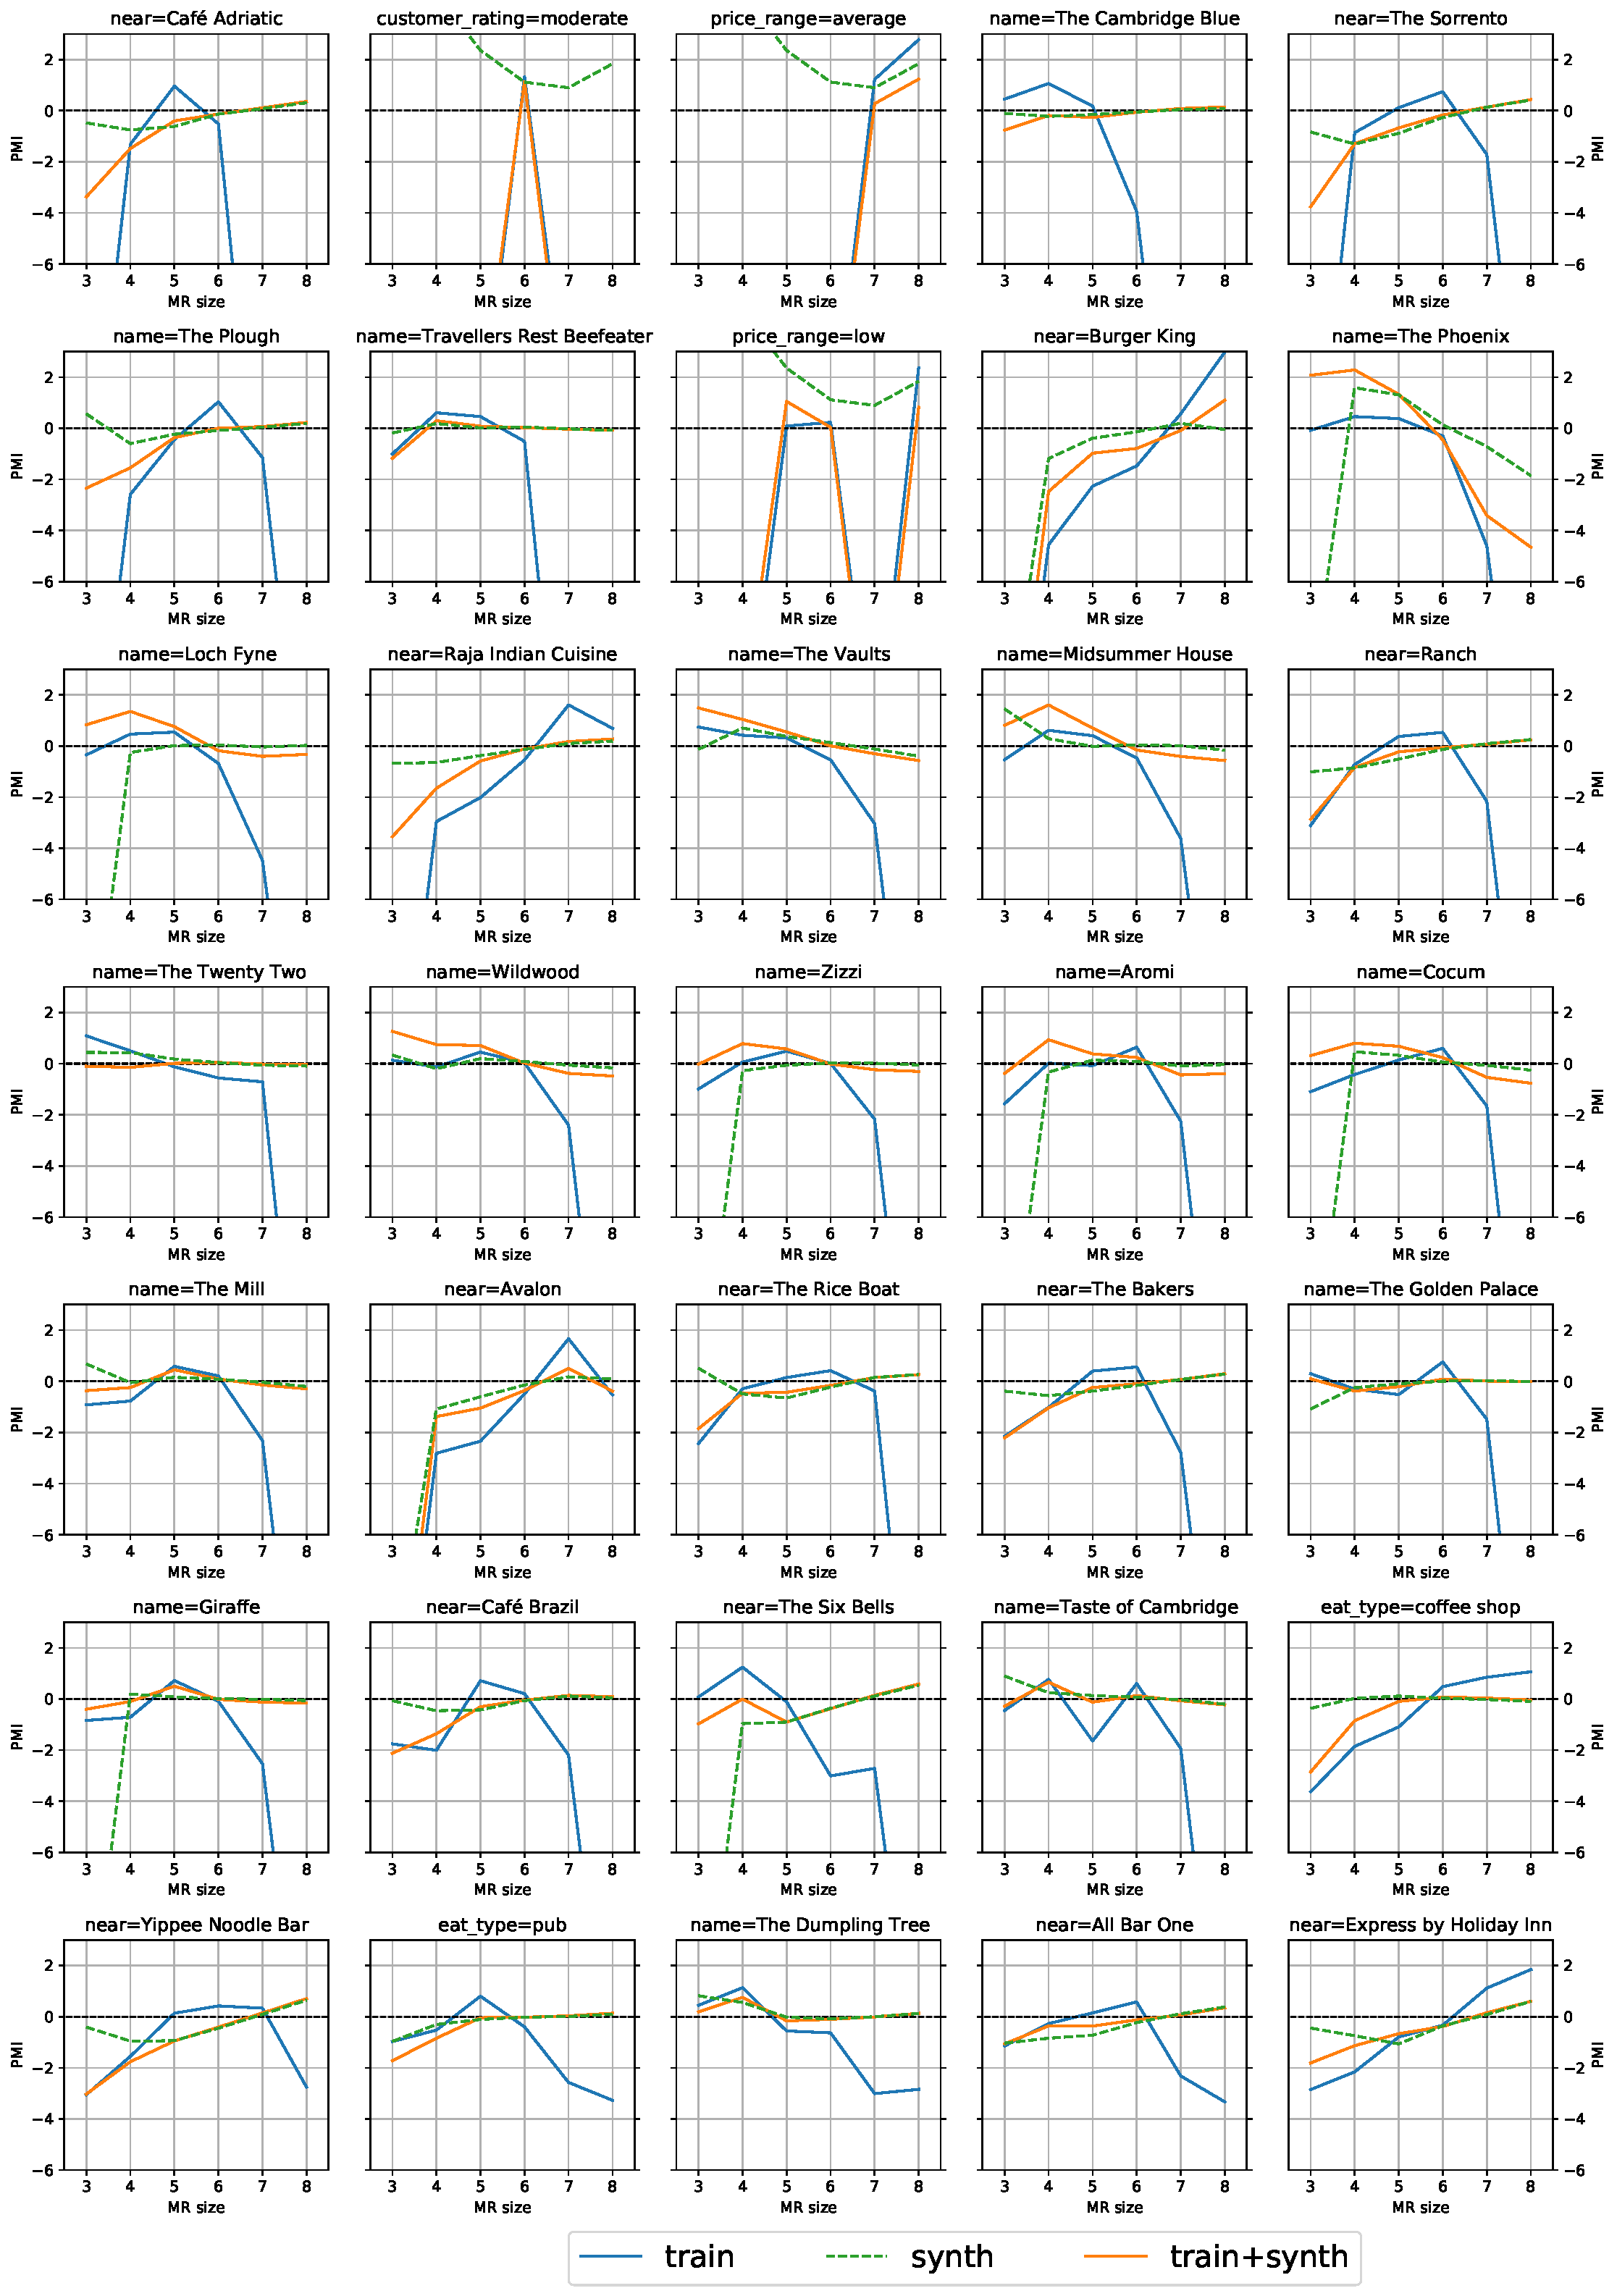
\includegraphics[width=0.9\textwidth]{ch5/figures/synthpmis.pdf}
\caption{PMI between various \attributevalue s and \meaningrepresentation~size
on the E2E Challenge dataset (blue), synthetic dataset (dashed green), and their union (orange). 0 on the $y$-axis indicates the two variables are independent.}
\label{fig:synthpmi}
\end{figure}


These recombinations are helpful. When we compare the PMI of various
\attributevalues~to \meaningrepresentation~size when using the original
training data (i.e., the plots we showed in \autoref{fig:bkpmi} and
\autoref{fig:trainpmi}) against the union of original and synthetic data
produced by noise-injection sampling (show in \autoref{fig:synthpmi}), we see
that most plots are much closer to 0 with the union of datasets, indicative of
greater independence between length and a particular \attributevalue, and that
this spurious association has been lessened considerably if not removed.

\begin{figure}
\begin{tikzpicture}
\node[anchor=north west,fill=olive,minimum height=2cm,text width=9cm] at (-8.1,3.90) {};
\node[anchor=north west,fill=violet,minimum height=2cm,text width=9cm] at (-8.1,3.75) {};
\node[anchor=north west,fill=blue,minimum height=2cm,text width=9cm] at (-8.1,3.23) {};
\node[anchor=north west,fill=purple,minimum height=2cm,text width=9cm] at (-8.1,3.0) {};
\node[anchor=north west,fill=green,minimum height=2cm,text width=9cm] at (-8.1,2.85) {};
\node[anchor=north west,fill=orange,minimum height=3cm,text width=9cm] at (-8.1,2.33) {};
\node[anchor=north west,fill=lime,minimum height=2cm,text width=9cm] at (-8.1,-.20) {};
\node[anchor=north west,fill=red,minimum height=0.59cm,text width=9cm] at (-8.1,-1.65) {};


\node[anchor=north west,fill=olive,minimum height=2cm,text width=0.1mm] at (0.33-7.35,-2.10) {};
\node[anchor=north west,fill=violet,minimum height=2cm,text width=2.8mm] at (0.48-7.35,-2.10) {};
\node[anchor=north west,fill=blue,minimum height=2cm,text width=2.8mm] at (1.0-7.35,-2.10) {};
\node[anchor=north west,fill=purple,minimum height=2cm,text width=2.8mm] at (1.22-7.35,-2.10) {};
\node[anchor=north west,fill=green,minimum height=2cm,text width=2.8mm] at (1.38-7.35,-2.10) {};
\node[anchor=north west,fill=orange,minimum height=2cm,text width=35.8mm] at (1.90-7.35,-2.10) {};
\node[anchor=north west,fill=lime,minimum height=2cm,text width=16.8mm] at (4.45-7.35,-2.10) {};
\node[anchor=north west,fill=red,minimum height=2cm,text width=3.3mm] at (5.86-7.35,-2.10) {};




\node[anchor=north west,fill=olive,minimum height=2cm,text width=0.1mm] at (0.33,-2.10) {};
\node[anchor=north west,fill=violet,minimum height=2cm,text width=2.8mm] at (0.48,-2.10) {};
\node[anchor=north west,fill=blue,minimum height=2cm,text width=2.8mm] at (1.0,-2.10) {};
\node[anchor=north west,fill=purple,minimum height=2cm,text width=2.8mm] at (1.22,-2.10) {};
\node[anchor=north west,fill=green,minimum height=2cm,text width=2.8mm] at (1.38,-2.10) {};
\node[anchor=north west,fill=orange,minimum height=2cm,text width=35.8mm] at (1.90,-2.10) {};
\node[anchor=north west,fill=lime,minimum height=2cm,text width=16.8mm] at (4.45,-2.10) {};
\node[anchor=north west,fill=red,minimum height=2cm,text width=3.3mm] at (5.86,-2.10) {};
\node at (0,0) {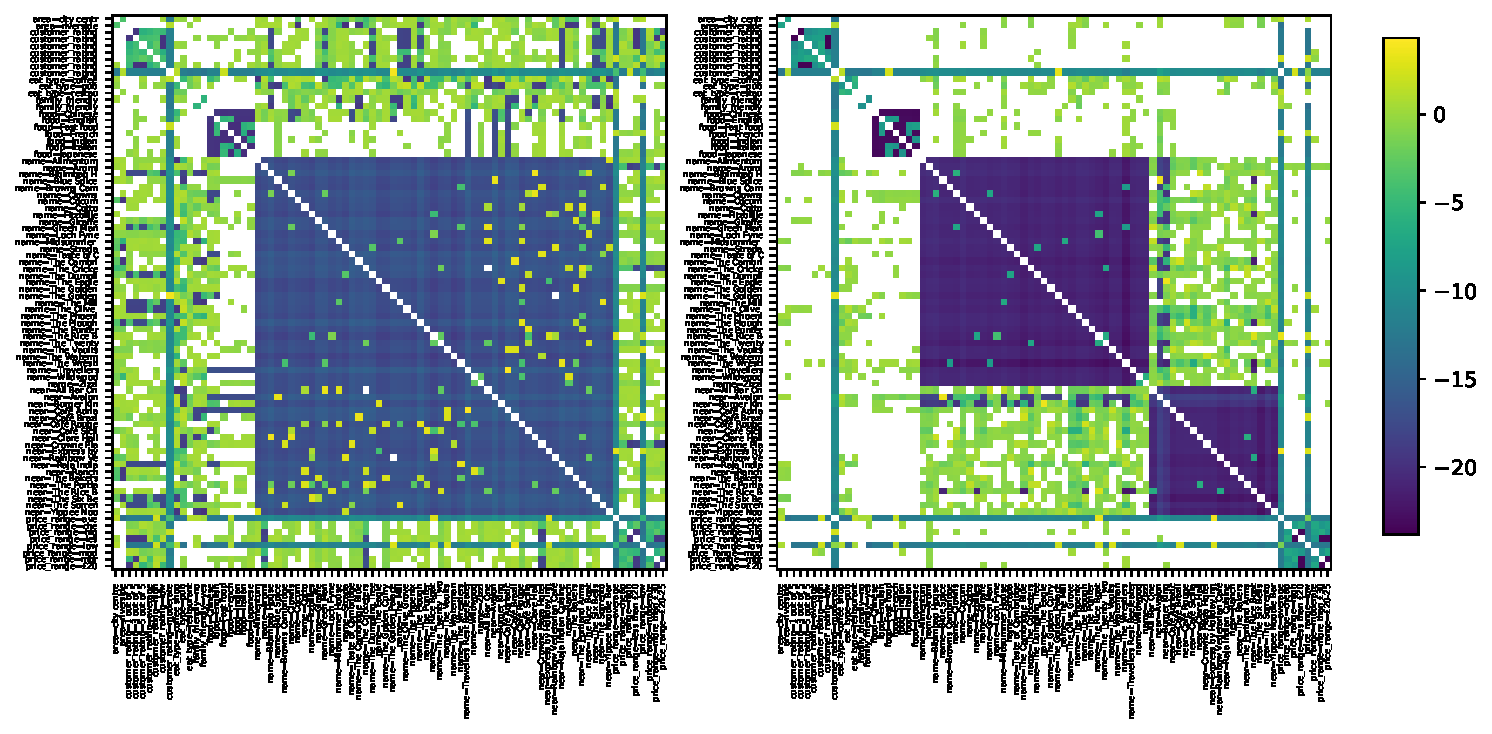
\includegraphics[width=\textwidth]{ch5/figures/heatmap_train.pdf}};
\end{tikzpicture}
\caption{PMI between E2E Challenge attribute-values on the original training data (left) and the union of the training and synthetic data (right). PMI between $(-.25,.25)$ are colored white and suggest relative independence between the two attribute-value pairs. Color blocks on the $x$ and $y$ axis labels correspond to groups of values for the same attribute. E.g., orange are all the values for the \Atr{name}~attribute.}
\label{fig:avpmi}
\end{figure}


Length is not the only spurious correlation present in the original training
dataset that can be mitigated by the synthetic datasets. In \autoref{fig:avpmi}
we plot the PMI between the occurrence of any two \attributevalues, e.g.
PMI(name=The Eagle,near=Burger King), on the original training data and union
of original and synthetic data.  Anti-correlation, i.e. extremely negative PMI
values, along the diagonal are expected as attribute-values in the E2E
Challenge dataset are mutually exclusive and don't usually co-occur (modulo
human annotator error).  We show PMI in the range of $(-.25, .25)$ as white
indicating roughly no strong association. In the ideal dataset, aside from
anti-correlation among values for the same attribute, we would like most the
PMI values to be close to 0. When comparing the PMI from the original dataset
(left) the union of original and synthetic, we see much more whitespace in the
latter suggesting there are fewer spurious associations between
\attributevalues~on the union dataset.

Producing training datasets with fewer spurious associations appears to be
highly beneficial when training \sequencetosequence~models for text generation
as we observe reduced semantic errors, and improved performance of greedy
decoding compared to more computationally intensive inference procedures.

\section{Alignment Training for Controllable Generation}
\label{sec:nlgcg}

In the previous section, we showed how to make an arbitrary
\sequencetosequence~model more likely to generate semantically correct
utterances using data-augmentation. While the resultant generation model is
more faithful, it still lacks even coarse-grained control over the organization
of the generated utterance.  What's more, there's no guarantee that small
changes to the input don't lead to dramatically different outputs.  For
example, changing a boolean attribute, e.g. changing
\AV{\textit{family\_friendly}}{\textit{yes}} to
\AV{\textit{family\_friendly}}{\textit{no}}, may lead to dramatically different
syntactic structure in the output.  This is because the structure or plan of
the utterance is only determined implicitly by the
\sequencetosequence~decoder's language model.

In this section, we show how to make a \sequencetosequence~controllable, which
we achieve through a particular linearization of the input
\meaningrepresentation, a linearization strategy we call \textit{alignment
training}. That is, we can specify the order in which the \attributevalues~of
an input \meaningrepresentation~are to be realized in the utterance.  See
\autoref{fig:examplecontrol} for example realizations from a controllable
generation model that follow three different permutations of \Atr{name},
\Atr{eat\_type}, and \Atr{area} attributes.  Through evaluation on two dialogue
generation benchmarks we show that alignment training yields high levels of
control in both GRU and Transformer models. This holds when models follow
either a separate planning model or a human provided plan.

We also propose using a phrase-based data augmentation method to further
improve the robustness of control. We further evaluate the control mechanism on
randomly generated plans which are much harder to follow than human or model
provided plans. We find that phrase-based data augmentation helps
\sequencetosequence~models follow these more difficult plans.

\subsection{Alignment Training Linearization}

Unlike the arbitrary linearization used in \autoref{sec:fgtgm},
\alignmenttraining~linearization~is not solely a function of $\mr$, but is
determined by both $\mr$ and a reference utterance $\utttoks$. Given a
$\left(\mr, \utttoks\right)$ pair, the \alignmenttraining~linearization finds a
linearization $\ls$ such that the order of the \attributevalues~in $\ls(\mr)$
corresponds to the order in which they are realized in $\utttoks$. 

\begin{figure}[p]
    \fbox{\begin{minipage}{\textwidth}
\center

\begin{minipage}{0.98\textwidth}
\begin{subfigure}{\textwidth}
\caption{Example of an alignment training linearization for a \meaningrepresentation~with a list-valued attribute, \textit{genres}. Note also that the \textit{rating} attribute for ViGGO examples is not aligned but always appended after the dialogue act (see \autoref{sec:align} for details). }
\center
\begin{minipage}[t]{0.48\textwidth}
\small
$\mr = \left[\!\!\left[\begin{array}{l} 
    \textsc{Give Opinion} \\ 
    \textrm{name=Little Nightmares} \\
    \textrm{rating=good} \\
    \textrm{genres=[}\\
    \textrm{~~~~adventure,} \\
    \textrm{~~~~platformer,}\\
    \textrm{~~~~puzzle} \\
    \textrm{]} \\
    \textrm{player\_perspective=side view}
\end{array}\right]\!\!\right]$ 
\end{minipage}
\hfill
\begin{minipage}[t]{0.48\textwidth}
\small
$\ls(\mr) = \left[ \begin{array}{l}
\starttok, \\
\textit{give\_opinion},\\
\textit{rating=good},\\ 
\textit{name=Little Nightmares},  \\
\textit{genres=adventure},  \\
\textit{player\_perspective=side view},\\
\textit{genres=platformer},  \\
\textit{genres=puzzle},  \\
\stoptok\end{array} \right]
$ 
\end{minipage}\\
\begin{minipage}[t]{\textwidth}
~\\[0pt]
$\utttoks = $ \textit{Little Nightmares is a pretty cool game that has kept me entertained. It's an adventure side-scrolling platformer with some puzzle elements to give me a bit of a challenge.}
\end{minipage}
\end{subfigure}

~\\~\\


\begin{subfigure}{\textwidth}
\caption{Example of an alignment training linearization with repeated attribute-values. In this case, the \textit{name} attribute is realized twice and 
so it appears twice in the linearization.}
\center
\begin{minipage}[t]{0.48\textwidth}
\small
$\mr = \left[\!\!\left[\begin{array}{l} 
    \textsc{Inform}\\
    {\AV{name}{Aromi}}\\
    {\AV{eat\_type}{coffee shop}}\\
    {\AV{customer\_rating}{5 out of 5}}\\
    {\AV{food}{English}}\\
    {\AV{area}{city centre}}\\
    {\AV{family\_friendly}{yes}}\\
\end{array} \right]\!\!\right]$
\end{minipage}
 \hfill
\begin{minipage}[t]{0.48\textwidth}
\small
$\ls(\mr) = \left[ \begin{array}{l}
\starttok, \\
\textit{inform},\\
\textit{name=Aromi},\\
\textit{eat\_type=coffee shop},\\
\textit{family\_friendly=yes},\\
\textit{food=English},\\
\textit{name=Aromi},\\
\textit{customer\_rating=5 out of 5},\\
\textit{area=city centre},\\
\stoptok\end{array} \right]
$ 
\end{minipage}\\
\begin{minipage}[t]{\textwidth}
~\\[0pt]
$\utttoks = $ \textit{The Aromi coffee shop is family-friendly and serves English food.  Aromi has a customer rating of 5 out of 5 and is located near the center of the city.}
\end{minipage}
\end{subfigure}

~\\~\\


\begin{subfigure}{\textwidth}
\caption{Example alignment training linearization where an attribute-value 
is not grounded in the reference utterance. In this case, \textit{food=Japanese}
is not present in the linearization.}
\center
\begin{minipage}[t]{0.48\textwidth}
\small
$\mr = \left[\!\!\left[\begin{array}{l} 
    \textsc{Inform}\\
    {\AV{name}{The Waterman}}\\
    {\AV{food}{Japanese}}\\
    {\AV{price\_range}{high}}\\
    {\AV{area}{riverside}}\\
\end{array} \right]\!\!\right]$
\end{minipage}
 \hfill
\begin{minipage}[t]{0.48\textwidth}
\small
$\ls(\mr) = \left[ \begin{array}{l}
\starttok, \\
\textit{inform},\\
\textit{area=riverside},\\
\textit{price\_range=high},\\
\textit{name=The Waterman},\\
\stoptok\end{array} \right]
$ 
\end{minipage}\\
\begin{minipage}[t]{\textwidth}
~\\[0pt]
$\utttoks = $ \textit{Near the river there is an expensive sushi place
called the Waterman.}
\end{minipage}
%\end{itemize}
%\label{fig:mr1utt}
\end{subfigure}
\end{minipage}
\end{minipage}}
\caption{Example \meaningrepresentation/utterance pairs ($\mr, \utttoks$) and their alignment
training linearization $\ls(\mr)$.}
\label{fig:atlexamples}
\end{figure}



\autoref{fig:atlexamples} shows some examples of the
\alignmenttraining~linearization, including some special cases. When
linearizing list-valued attributes, for instance, we treat them as distinct
\attributevalue~pairs
(\hyperref[fig:atlexamples]{\autoref{fig:atlexamples}.a}). Occasionally, we
encounter repeated \attributevalues~in the training set, and in that case we
include extra \attributevalue~pairs in the corresponding location in the
linearization (\hyperref[fig:atlexamples]{\autoref{fig:atlexamples}.b}). We
also ignore any instances of  ungrounded information, as in example
\hyperref[fig:atlexamples]{\autoref{fig:atlexamples}.c} where
\textit{food=Japanese} is not mentioned in the reference utterance.  has no
explicit representation.  

In \autoref{fig:at} we show the steps of our procedure for obtaining the
alignment training linearization, given a reference utterance $\utttoks$.  The
first step is to tag the utterance tokens $\utttoks =
\left[\utttok_1,\ldots,\utttok_\uttSize\right]$ with a corresponding tag
sequence $\mrtags=\left[\mrtag_1,\ldots, \mrtag_\uttSize\right]$ where each tag
$\mrtag_i$ is equal to an \attributevalue~$\mrtok_j \in \mr$ or the null tag
$\nulltag$. We assume that we have access to such a tagger $\tagger : \outSpace
\rightarrow \inSpace$ (see \autoref{sec:align} for implementation details).
After producing the tag sequence $\mrtags^{(1)} = \tagger\left(\utttoks\right)$
(\hyperref[fig:at]{\autoref{fig:at}b}), we then group contiguous sequences of
tags sharing the same tag value, discarding any null tag sequences to obtain
the sequence of subsequences $\mrtags^{(2)} =
\left[\mrtags^{(1)}_{i_1:j_1},\ldots,\mrtags^{(1)}_{i_\mrSize:j_\mrSize},
\right]$ (\hyperref[fig:at]{\autoref{fig:at}c}).  Finally, $\mrtoks$ is
constructed by by prepending the \dialogueact~$\mrtok_0$ of $\mr$ to the
ordered sequence of \attributevalue~pairs $\mrtok_1,\ldots,\mrtok_\mrSize$
implied by $\mrtags^{(1)}_{i_1},\ldots,\mrtags^{(1)}_{i_\mrSize}$
(\hyperref[fig:at]{\autoref{fig:at}d}). 

\tikzset{mynode/.style={anchor=center, minimum height=1.5em, 
      text height=1.5ex, text depth=.25ex, align=center}}

      \begin{figure}[p]
    \fbox{\begin{minipage}{\textwidth}
            ~\\
        \center
        \scalebox{0.75}{
    \begin{tikzpicture}
        \def\titlex{-3.0}
        \def\colwidth{1.25}
        \def\utttitleheight{2}
        \def\uttheightA{0.0}
        \def\uttheightB{-1.0}
        \def\tagtitleheight{-3.0}
        \def\tagheightA{-5.0}
        \def\tagheightB{-6.0}
        \def\nullsegtitleheight{-12.0}
        \def\nullsegheightA{-14.0}
        \def\mrsegtitleheight{-12.0}
        \def\mrsegheightA{-14.0}
        \def\attitleheight{-16.0}
        \def\atheightA{-18.0}
        \def\atheightB{-19.0}



        \def\city{{area=city centre}};
        \def\coffee{{eat\_type=coffee shop}};
       % \def\nulltag{{$\emptyset$}};
        \def\name{{name=Aromi}};
        \def\words{For, coffee, in, the, centre, of, the, city, {,}, try, 
                   Aromi, .};
        \def\tags{\coffee, \coffee, \city, \city, \city, \city, \city, \city,
                     \nulltag, \nulltag, \name, \nulltag};

        %%% Input Utterance
        \node[mynode,anchor=west] at (\titlex*\colwidth,\utttitleheight) 
            {\Large (a) Input Utterance};

        \foreach \w [count=\wi from 1] in \words {
            \node[mynode] at (\wi*\colwidth,\uttheightA) 
                {$\utttok_{\wi}\ifthenelse{\wi = 12}{}{,}$};
            \node[mynode] at (\wi*\colwidth,\uttheightB) {\w};
        }
        \node[mynode] at (0*\colwidth,\uttheightA) {$\utttoks = \Bigg[$};
        \node[mynode] at (12*\colwidth+0.5,\uttheightA) {$\Bigg]$};


        %%% Tagged Utterance
        \node[mynode,anchor=west] at (\titlex*\colwidth,\tagtitleheight) 
            {\Large (b) Tagged Utterance};
        \foreach \t [count=\ti from 1] in \tags {
            \node[mynode] at (\ti*\colwidth,\tagheightA) 
                {$\mrtag_{\ti}\ifthenelse{\ti = 12}{}{,}$};
            \node[mynode,rotate=90,anchor=east] at 
                (\ti*\colwidth,\tagheightB) {\t};
        }
        \node[mynode] at (0*\colwidth,\tagheightA) {$\mrtags^{(1)} = \Bigg[$};
        \node[mynode] at (12*\colwidth+0.5,\tagheightA) {$\Bigg]$};


%        %%% Null Segmented Tags
%        \node[mynode,anchor=west] at (\titlex*\colwidth,\nullsegtitleheight) 
%            {\Large (c) Null Segmented Tags};
%        \node[mynode] at (0*\colwidth,\nullsegheightA) 
%            {$\mrtags^{(2)} = \Bigg[$};
%        \node[mynode] at (12*\colwidth+0.5,\nullsegheightA) {$\Bigg]$};        
%        \foreach \tprime in {1,...,8} {
%            \node[mynode] at (\tprime*\colwidth,\nullsegheightA) 
%            {$\mrtag_{\tprime}\ifthenelse{\tprime = 8}{}{,}$};
%        }
%        \foreach \tprime in {11} {
%            \node[mynode] at (\tprime*\colwidth,\nullsegheightA) 
%                {$\mrtag_{\tprime}$};
%        }
%
%        \node[mynode] at (\colwidth-0.50,\nullsegheightA) {$\bigg[$};
%        \node[mynode] at (8*\colwidth+0.50,\nullsegheightA) {$\bigg],$};
%        \node[mynode] at (11*\colwidth-0.50,\nullsegheightA) {$\bigg[$};
%        \node[mynode] at (11*\colwidth+0.50,\nullsegheightA) {$\bigg]$};


        %%% MR Segmented Tags
        \node[mynode,anchor=west] at (\titlex*\colwidth,\mrsegtitleheight) 
            {\Large (c) MR Segmented Tags};
        \node[mynode] at (0*\colwidth,\mrsegheightA) 
            {$\mrtags^{(2)} = \Bigg[$};
        \node[mynode] at (12*\colwidth+0.5,\mrsegheightA) {$\Bigg]$};        
        \foreach \tprime in {1,...,2} {
            \node[mynode] at (\tprime*\colwidth,\mrsegheightA) 
            {$\mrtag_{\tprime}\ifthenelse{\tprime = 2}{}{,}$};
        }
        \foreach \tprime in {3,...,8} {
            \node[mynode] at (\tprime*\colwidth,\mrsegheightA) 
            {$\mrtag_{\tprime}\ifthenelse{\tprime = 8}{}{,}$};
        }
        \foreach \tprime in {11} {
            \node[mynode] at (\tprime*\colwidth,\mrsegheightA) 
                {$\mrtag_{\tprime}$};
        }

        \node[mynode] at (\colwidth-0.50,\mrsegheightA) {$\bigg[$};
        \node[mynode,anchor=center] at (2*\colwidth+0.65,\mrsegheightA) {$\Bigg]_1, \Bigg[$};
    \node[mynode] at (8*\colwidth+0.50,\mrsegheightA) {$\bigg]_2,$};
        \node[mynode] at (11*\colwidth-0.50,\mrsegheightA) {$\bigg[$};
        \node[mynode] at (11*\colwidth+0.50,\mrsegheightA) {$\bigg]_3$};


        %%% Alignment Training Linearization
        \node[mynode,anchor=west] at (\titlex*\colwidth,\attitleheight) 
            {\Large (d) Alignment Training Linearization};
        \node[mynode,anchor=east] at (-1.5*\colwidth-0.5,\atheightA) 
            {$\mrtoks = \Bigg[$};
        \node[mynode] at (-1.5*\colwidth,\atheightA) {$\mrtok_0,$};
        \node[mynode] at (1.5*\colwidth,\atheightA) {$\mrtok_1,$};
        \node[mynode] at (5.5*\colwidth,\atheightA) {$\mrtok_2,$};
        \node[mynode] at (11*\colwidth,\atheightA) {$\mrtok_3$};
        \node[mynode] at (11*\colwidth+0.5,\atheightA) {$\Bigg]$};
%
        \node[mynode] at (-1.5*\colwidth,\atheightB) {inform,};
        \node[mynode] at (1.5*\colwidth,\atheightB) {eat\_type=coffee shop,};
        \node[mynode] at (5.5*\colwidth,\atheightB) {area=city centre,};
        \node[mynode] at (11*\colwidth,\atheightB) {name=Aromi};



    \end{tikzpicture}
    }
    ~\\
    \caption{Example steps of the \alignmenttraining~linearization algorithm
        for producing a linearized \meaningrepresentation~$\mrtoks$.}
        \label{fig:at}
\end{minipage}}
\end{figure}




At test time, the generation model is only presented with a
\meaningrepresentation~$\mr$ and we don't have a reference utterance $\utttoks$
with which to apply the alignment training linearization. In this case, we can
use an utterance planning model $\planner : \mrspace \rightarrow \inSpace$ to
map a \meaningrepresentation~$\mr$ to a linear sequence $\mrtoks$.
Alternatively, we can use the test set reference to obtain the alignment
training linearization; this represents an unrealistically optimistic case
where the model has clairvoyant known of the discourse ordering preferred by a
human.  In either case, we refer to a linearization $\mrtoks$ obtained either
from $\planner$ or a human reference as an \utteranceplan~since a generation
model trained with \alignmenttraining~linearizations will attempt to follow it
during the generation of the utterance.

\subsubsection{Alternative Linearization Strategies}

In our experiments, we compare alignment training to three other linearization
strategies, which we describe below.  These linearizations, while sensible
methods of mapping a \meaningrepresentation~to a linear sequence of tokens,
have no correspondence between the \meaningrepresentation~linearization and
surface realization order. Because of this, \sequencetosequence~models trained
using these linearization strategies are not controllable. These linearization
strategies may have some effect on the faithfulness when compared to each other
and alignemnt training, so evaluation of this modelling choice has additional
benefits beyond benchmarking alignment training.  See \autoref{fig:linstrats}
for examples of the different linearization strategies on the same
\meaningrepresentation/utterance pair.

\paragraph{Random (\textsc{Rnd})} In the \textsc{Random} linearization
(\textsc{Rnd}), we randomly order the attribute-value pairs for a given
\meaningrepresentation. This strategy serves as a baseline for determining if
linearization ordering matters at all for faithfulness. \textsc{Rnd} is similar
to token level noise used in sequential denoising autoencoders
\citep{wang2019denoising} and might even improve faithfulness.  During
training, we resample the ordering for each example at every epoch so as not to
over fit to a particular random ordering.  We do not resample the validation
set in order to obtain stable results from which to pick the best model.


\newtcbox{\mybox}[1][]{colframe=blue, colback=blue!15, 
                       nobeforeafter, tcbox raise base, shrink tight, extrude 
                       by=0.75mm, #1}



\begin{figure}
    \center
    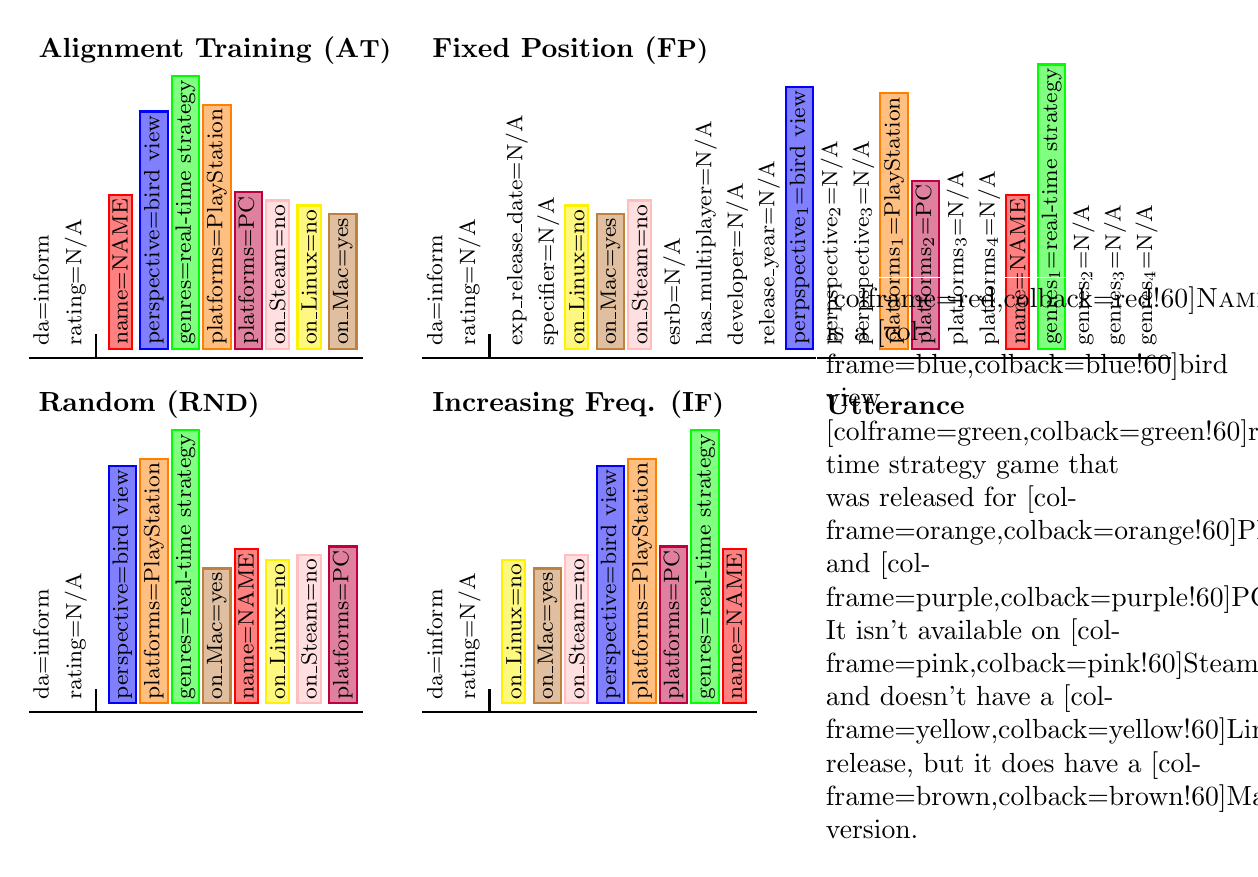
\begin{tikzpicture}[]


    \node[anchor=west] at (5.0,5.8) 
        {\textbf{Fixed Position \textsc{(F\small{P})}}};
    \node[anchor=west] at (0.0,5.8) 
        {\textbf{Alignment Training \textsc{(A\small{T})}}};
    \draw[thick] (0.85,1.9) -- (0.85,2.2);
    \draw[thick] (0,1.9) -- (4.25,1.9);
    \draw[thick] (5 + 0.85,1.9) -- (5 + 0.85,2.2);
    \draw[thick] (5 + 0,1.9) -- (10.25+ 4.25,1.9);
    \draw[thick] (0.85,-2.6) -- (0.85,-2.3);
    \draw[thick] (0,-2.6) -- (4.25,-2.6);
    \draw[thick] (5+0.85,-2.6) -- (5+0.85,-2.3);
    \draw[thick] (5+0,-2.6) -- (5+4.25,-2.6);

    \node[anchor=north west,inner sep=0.5mm,rotate=90] at (0,2) 
        {\footnotesize da=inform};
    \node[anchor=north west,inner sep=0.5mm,rotate=90] at (0.4,2) 
        {\footnotesize rating=N/A};
    \node[anchor=north west,rotate=90,inner sep=0.5mm,draw=red,thick,fill=red!50] 
        at (0.2 + 0.8,2) 
        {\footnotesize name=NAME};
    \node[anchor=north west,rotate=90,inner sep=0.5mm,draw=blue,thick,fill=blue!50] 
        at (0.2 + 1.2,2) {\footnotesize perspective=bird view};
    \node[anchor=north west,rotate=90,inner sep=0.5mm,draw=green,thick,
          fill=green!50] 
        at (0.2 + 1.6,2) {\footnotesize genres=real-time strategy};
    \node[anchor=north west,rotate=90,inner sep=0.5mm,draw=orange,thick,
          fill=orange!50] 
        at (0.2 + 2.0,2) {\footnotesize platforms=PlayStation};
    \node[anchor=north west,rotate=90,inner sep=0.5mm,draw=purple,thick,
          fill=purple!50] 
        at (0.2 + 2.4,2) {\footnotesize platforms=PC};
    \node[anchor=north west,rotate=90,inner sep=0.5mm,draw=pink,thick,
          fill=pink!50] 
        at (0.2 + 2.8,2) {\footnotesize on\_Steam=no};
    \node[anchor=north west,rotate=90,inner sep=0.5mm,draw=yellow,thick,
          fill=yellow!50] 
        at (0.2 + 3.2,2) {\footnotesize on\_Linux=no};
    \node[anchor=north west,rotate=90,inner sep=0.5mm,draw=brown,thick,
          fill=brown!50] 
        at (0.2 + 3.6,2) {\footnotesize on\_Mac=yes};


\node[anchor=north west,inner sep=0.5mm,rotate=90] at (5 + 0,2) 
    {\footnotesize da=inform};
\node[anchor=north west,inner sep=0.5mm,rotate=90] at (5 + 0.4,2) 
    {\footnotesize rating=N/A};
\node[anchor=north west,rotate=90,inner sep=0.5mm] 
    at (5.2 + 0.8,2) 
    {\footnotesize exp\_release\_date=N/A};
\node[anchor=north west,rotate=90,inner sep=0.5mm] 
    at (5.2 + 1.2,2) 
    {\footnotesize specifier=N/A};
\node[anchor=north west,rotate=90,inner sep=0.5mm,draw=yellow,thick,fill=yellow!50] 
    at (5.2 + 1.6,2) 
    {\footnotesize on\_Linux=no};
\node[anchor=north west,rotate=90,inner sep=0.5mm,draw=brown,thick,fill=brown!50] 
    at (5.2 + 2.0,2) 
    {\footnotesize on\_Mac=yes};
\node[anchor=north west,rotate=90,inner sep=0.5mm,draw=pink,thick,fill=pink!50] 
    at (5.2 + 2.4,2) 
    {\footnotesize on\_Steam=no};
\node[anchor=north west,rotate=90,inner sep=0.5mm] 
    at (5.2 + 2.8,2) 
    {\footnotesize esrb=N/A};
\node[anchor=north west,rotate=90,inner sep=0.5mm] 
    at (5.2 + 3.2,2) 
    {\footnotesize has\_multiplayer=N/A};

   % ['inform', 'rating=N/A', 'exp_release_date=N/A', 'specifier=N/A', 'has_linux_release=no', 'has_mac_release=yes', 'available_on_steam=no', 'esrb=N/A', 'has_multiplayer=N/A', 'developer=N/A', 'release_year=N/A', 'player_perspective=bird view', 'player_perspective=N/A', 'player_perspective=N/A', 'platforms=PlayStation', 'platforms=PC', 'platforms=N/A', 'platforms=N/A', 'name=PLACEHOLDER', 'genres=real-time strategy', 'genres=N/A', 'genres=N/A', 'genres=N/A']
\node[anchor=north west,rotate=90,inner sep=0.5mm] 
    at (5.2 + 3.6,2) 
    {\footnotesize developer=N/A};
\node[anchor=north west,rotate=90,inner sep=0.5mm] 
    at (5.2 + 4.0,2) 
    {\footnotesize release\_year=N/A};
\node[anchor=north west,rotate=90,inner sep=0.5mm,draw=blue,thick,fill=blue!50] 
    at (5.2 + 4.4,2) 
    {\footnotesize perpspective\textsubscript{1}=bird view};
\node[anchor=north west,rotate=90,inner sep=0.5mm] 
    at (5.2 + 4.8,2) 
    {\footnotesize perpspective\textsubscript{2}=N/A};
\node[anchor=north west,rotate=90,inner sep=0.5mm] 
    at (5.2 + 5.2,2) 
    {\footnotesize perpspective\textsubscript{3}=N/A};
\node[anchor=north west,rotate=90,inner sep=0.5mm,draw=orange,thick,fill=orange!50] 
    at (5.2 + 5.6,2) 
    {\footnotesize platforms\textsubscript{1}=PlayStation};
\node[anchor=north west,rotate=90,inner sep=0.5mm,draw=purple,thick,fill=purple!50] 
    at (5.2 + 6.0,2) 
    {\footnotesize platforms\textsubscript{2}=PC};
\node[anchor=north west,rotate=90,inner sep=0.5mm] 
    at (5.2 + 6.4,2) 
    {\footnotesize platforms\textsubscript{3}=N/A};
\node[anchor=north west,rotate=90,inner sep=0.5mm] 
    at (5.2 + 6.8,2) 
    {\footnotesize platforms\textsubscript{4}=N/A};
\node[anchor=north west,rotate=90,inner sep=0.5mm,draw=red,thick,fill=red!50] 
    at (5.2 + 7.2,2) 
    {\footnotesize name=NAME};
\node[anchor=north west,rotate=90,inner sep=0.5mm,draw=green,thick,fill=green!50] 
    at (5.2 + 7.6,2) 
    {\footnotesize genres\textsubscript{1}=real-time strategy};
\node[anchor=north west,rotate=90,inner sep=0.5mm] 
    at (5.2 + 8.0,2) 
    {\footnotesize genres\textsubscript{2}=N/A};
\node[anchor=north west,rotate=90,inner sep=0.5mm] 
    at (5.2 + 8.4,2) 
    {\footnotesize genres\textsubscript{3}=N/A};
\node[anchor=north west,rotate=90,inner sep=0.5mm] 
    at (5.2 + 8.8,2) 
    {\footnotesize genres\textsubscript{4}=N/A};


%\node[anchor=north west,rotate=90] at (1.5,2) {genres=platformer};
%\node[anchor=north west,rotate=90] at (2,2) {genres=puzzle};
%\node[anchor=north west,rotate=90] at (2.5,2) {perspective=side vew};
%\node[anchor=north west,rotate=90] at (3,2) {name=NAME};
%\node[anchor=north west,rotate=90] at (3.5,2) {name=NAME};
%\node[anchor=north west,rotate=90] at (4,2) {name=NAME};
%\node[anchor=north west,rotate=90] at (4.5,2) {name=NAME};
%
%
%\node[anchor=north west,rotate=90] at (5.5+0,2) {\small give opinion};
%\node[anchor=north west,rotate=90] at (5.5+0.5,2) {\small rating=good};
%\node[anchor=north west,rotate=90] at (5.5+1,2) {\small genres=adventure};
%\node[anchor=north west,rotate=90] at (5.5+1.5,2) {genres=platformer};
%\node[anchor=north west,rotate=90] at (5.5+2,2) {genres=puzzle};
%\node[anchor=north west,rotate=90] at (5.5+2.5,2) {perspective=side vew};
%\node[anchor=north west,rotate=90] at (5.5+3,2) {name=NAME};
%\node[anchor=north west,rotate=90] at (5.5+3.5,2) {name=NAME};
%\node[anchor=north west,rotate=90] at (5.5+4,2) {name=NAME};
%\node[anchor=north west,rotate=90] at (10+0,2) {give opinion};
%\node[anchor=north west,rotate=90] at (10+0.5,2) {rating=good};
%\node[anchor=north west,rotate=90] at (10+1,2) {genres=adventure};
%\node[anchor=north west,rotate=90] at (10+1.5,2) {genres=platformer};
%\node[anchor=north west,rotate=90] at (10+2,2) {genres=puzzle};
%\node[anchor=north west,rotate=90] at (10+2.5,2) {perspective=side vew};
%\node[anchor=north west,rotate=90] at (10+3,2) {name=NAME};
%\node[anchor=north west,rotate=90] at (10+3.5,2) {name=NAME};
%\node[anchor=north west,rotate=90] at (10+4,2) {name=NAME};
%\node[anchor=north west,rotate=90] at (10+4.5,2) {name=NAME};
%
%



%['give_opinion', 'rating=good', 'genres=adventure', 'genres=platformer', 'genres=puzzle', 'player_perspective=side view', 'name=PLACEHOLDER']


%#
%#

%['inform', 'rating=N/A', 'exp_release_date=N/A', 'specifier=N/A', 'has_linux_release=no', 'has_mac_release=yes', 'available_on_steam=no', 'esrb=N/A', 'has_multiplayer=N/A', 'developer=N/A', 'release_year=N/A', 'player_perspective=bird view', 'player_perspective=N/A', 'player_perspective=N/A', 'platforms=PlayStation', 'platforms=PC', 'platforms=N/A', 'platforms=N/A', 'name=PLACEHOLDER', 'genres=real-time strategy', 'genres=N/A', 'genres=N/A', 'genres=N/A']


%inc_freq_delex
%['inform', 'rating=N/A', 'has_linux_release=no', 'has_mac_release=yes', 'available_on_steam=no', 'player_perspective=bird view', 'platforms=PlayStation', 'platforms=PC', 'name=PLACEHOLDER', 'genres=real-time strategy']

\node[anchor=north west,inner sep=0.5mm,rotate=90] at (0,-2.5) 
    {\footnotesize da=inform};
\node[anchor=north west,inner sep=0.5mm,rotate=90] at (0.4,-2.5) 
    {\footnotesize rating=N/A};
\node[anchor=north west,rotate=90,inner sep=0.5mm,draw=blue,thick,fill=blue!50] 
    at (0.2 + 0.8,-2.5) 
    {\footnotesize perspective=bird view};

\node[anchor=north west,rotate=90,inner sep=0.5mm,draw=orange,thick,fill=orange!50] 
    at (0.2 + 1.2,-2.5) 
    {\footnotesize platforms=PlayStation};
\node[anchor=north west,rotate=90,inner sep=0.5mm,draw=green,thick,fill=green!50] 
    at (0.2 + 1.6,-2.5) 
    {\footnotesize genres=real-time strategy};


\node[anchor=north west,rotate=90,inner sep=0.5mm,draw=brown,thick,fill=brown!50] 
    at (0.2 + 2.0,-2.5) 
    {\footnotesize on\_Mac=yes};
\node[anchor=north west,rotate=90,inner sep=0.5mm,draw=red,thick,fill=red!50] 
    at (0.2 + 2.4,-2.5) 
    {\footnotesize name=NAME};

\node[anchor=north west,rotate=90,inner sep=0.5mm,draw=yellow,thick,fill=yellow!50] 
    at (0.2 + 2.8,-2.5) 
    {\footnotesize on\_Linux=no};
\node[anchor=north west,rotate=90,inner sep=0.5mm,draw=pink,thick,fill=pink!50] 
    at (0.2 + 3.2,-2.5) 
    {\footnotesize on\_Steam=no};
\node[anchor=north west,rotate=90,inner sep=0.5mm,draw=purple,thick,fill=purple!50] 
    at (0.2 + 3.6,-2.5) 
    {\footnotesize platforms=PC};

    \node[anchor=west] at (0,1.3) {\textbf{Random \textsc{(R\small{ND})}}};



\node[anchor=north west,inner sep=0.5mm,rotate=90] at (5 + 0,-2.5) 
    {\footnotesize da=inform};
\node[anchor=north west,inner sep=0.5mm,rotate=90] at (5 + 0.4,-2.5) 
    {\footnotesize rating=N/A};
\node[anchor=north west,rotate=90,inner sep=0.5mm,draw=yellow,thick,fill=yellow!50] 
    at (5.2 + 0.8,-2.5) 
    {\footnotesize on\_Linux=no};
\node[anchor=north west,rotate=90,inner sep=0.5mm,draw=brown,thick,fill=brown!50] 
    at (5.2 + 1.2,-2.5) 
    {\footnotesize on\_Mac=yes};
\node[anchor=north west,rotate=90,inner sep=0.5mm,draw=pink,thick,fill=pink!50] 
    at (5.2 + 1.6,-2.5) 
    {\footnotesize on\_Steam=no};

\node[anchor=north west,rotate=90,inner sep=0.5mm,draw=blue,thick,fill=blue!50]
    at (5.2 + 2.0,-2.5) 
    {\footnotesize perspective=bird view};
\node[anchor=north west,rotate=90,inner sep=0.5mm,draw=orange,thick,fill=orange!50] 
    at (5.2 + 2.4,-2.5) 
    {\footnotesize platforms=PlayStation};
\node[anchor=north west,rotate=90,inner sep=0.5mm,draw=purple,thick,fill=purple!50] 
    at (5.2 + 2.8,-2.5) 
    {\footnotesize platforms=PC};

\node[anchor=north west,rotate=90,inner sep=0.5mm,draw=green,thick,fill=green!50] 
    at (5.2 + 3.2,-2.5) 
    {\footnotesize genres=real-time strategy};
\node[anchor=north west,rotate=90,inner sep=0.5mm,draw=red,thick,fill=red!50] 
    at (5.2 + 3.6,-2.5) 
    {\footnotesize name=NAME};
%has_linux_release=no', 'has_mac_release=yes', 'available_on_steam=no', 'player_perspective=bird view', 'platforms=PlayStation', 'platforms=PC', 'name=PLACEHOLDER', 'genres=real-time strategy'
    \node[anchor=west] at (5.0,1.3) {\textbf{Increasing Freq. \textsc{(I\small{F})}}};


%\node[anchor=north west,inner sep=0.5mm,rotate=90] at (10 + 0,-2.5) 
%    {\footnotesize da=inform};
%\node[anchor=north west,inner sep=0.5mm,rotate=90] at (10 + 0.4,-2.5) 
%    {\footnotesize rating=N/A};
%
%\node[anchor=north west,rotate=90,inner sep=0.5mm,draw=red,thick,fill=red!50] 
%    at (10.2 + 0.8,-2.5) 
%    {\footnotesize name=NAME};
%
%\node[anchor=north west,rotate=90,inner sep=0.5mm,draw=green,thick,fill=green!50] 
%    at (10.2 + 1.2,-2.5) 
%    {\footnotesize genres=real-time strategy};
%
%    \node[anchor=north west,rotate=90,inner sep=0.5mm,draw=purple,thick,fill=purple!50] 
%    at (10.2 + 1.6,-2.5) 
%    {\footnotesize platforms=PC};
%\node[anchor=north west,rotate=90,inner sep=0.5mm,draw=orange,thick,fill=orange!50] 
%    at (10.2 + 2.0,-2.5) 
%    {\footnotesize platforms=PlayStation};
%
%\node[anchor=north west,rotate=90,inner sep=0.5mm,draw=blue,thick,fill=blue!50]
%    at (10.2 + 2.4,-2.5) 
%    {\footnotesize perspective=bird view};
%\node[anchor=north west,rotate=90,inner sep=0.5mm,draw=pink,thick,fill=pink!50] 
%    at (10.2 + 2.8,-2.5) 
%    {\footnotesize on\_Steam=no};
%\node[anchor=north west,rotate=90,inner sep=0.5mm,draw=brown,thick,fill=brown!50] 
%    at (10.2 + 3.2,-2.5) 
%    {\footnotesize on\_Mac=yes};
%\node[anchor=north west,rotate=90,inner sep=0.5mm,draw=yellow,thick,fill=yellow!50] 
%    at (10.2 + 3.6,-2.5) 
%    {\footnotesize on\_Linux=no};
%




%has_linux_release=no', 'has_mac_release=yes', 'available_on_steam=no', 'player_perspective=bird view', 'platforms=PlayStation', 'platforms=PC', 'name=PLACEHOLDER', 'genres=real-time strategy'
%    \node[anchor=west] at (10.0,1.3) {\textbf{Decreasing Freq.}};




    \node[anchor=west] at (10, 1.3) {\textbf{Utterance}};
\node[text width=5.0cm,draw=white,anchor=west] at (10,-0.7) {
    {\mybox[colframe=red,colback=red!60]{\textsc{Name}}} is a 
    \mybox[colframe=blue,colback=blue!60]{bird view} 
    \mybox[colframe=green,colback=green!60]{real-time strategy} 
    game that was released for 
    \mybox[colframe=orange,colback=orange!60]{PlayStation} and 
    \mybox[colframe=purple,colback=purple!60]{PC.} It isn't available on 
    \mybox[colframe=pink,colback=pink!60]{Steam} and doesn't have a 
    \mybox[colframe=yellow,colback=yellow!60]{Linux} release, but it does have
    a \mybox[colframe=brown,colback=brown!60]{Mac} version.
};


\end{tikzpicture}

\caption{Example \meaningrepresentation~linearization strategies for an utterance (lower right) from the 
    ViGGO training set.}
\label{fig:linstrats}
\end{figure}


\paragraph{Increasing Frequency (\textsc{If})} In the \textsc{Increasing
Frequency} linearization (\textsc{If}), we order the attribute-value pairs by
increasing frequency of occurrence in the training data i.e.
$\acount(\attr_i=\aval_i) \le \acount(\attr_{i+1}=\aval_{i+1})$.  We
hypothesize that placing frequently occurring items in a consistent location
may make it easier for the generation model to realize those items correctly,
possibly at the expense of rarer items.

\paragraph{Fixed Position (\textsc{Fp})} We take  consistency one step further
and create a fixed ordering of all attributes, \textit{n.b.} not
attribute-values, ordering them in increasing frequency of occurrence on the
training set (i.e. every instance has the same order of attributes in the
encoder input). In this \textsc{Fixed Position} linearization (\textsc{Fp}),
attributes that are not present in an \meaningrepresentation~are explicitly
represented with an \textit{N/A} value.  For list-valued slots, we determine
the maximum length list in the training data and create that many repeated
slots in the input sequence.  This linearization is feasible for datasets with
a modest number of unique attributes (in our case ViGGO has 14 attributes and
the E2E Challenge corpus has eight) but would not easily scale to 10s, 100s, or
larger attribute vocabularies. 

\subsection{Phrase-based Data Augmentation}
\label{sec:pbda}

\begin{figure}
    \centering


        \begin{tikzpicture}

            \def\th{5mm};
            \def\td{2mm};
    \node[text height=\th,text depth=\td] (aromi) at (-5,-4) {Aromi};
            \node[text height=\th,text depth=\td] (is) at (-1.5,-4) {is};
            \node[text height=\th,text depth=\td] (not) at (0.0,-4) {not};

            \node[text height=\th,text depth=\td] (a) at (1.5,-4) {a};
            \node[text height=\th,text depth=\td] (ff) at (4,-4) {family-friendly};
            \node[text height=\th,text depth=\td] (est) at (6.5,-4) {establishment};


            \node (root) at (-2.5,0) {S};
            \node[draw,circle,font=\small,inner sep=0] at ($(root)+(-0.5,0.5)$) {4};
            \node (rootNP) at (-5,-1) {NP};
            \node[draw,circle,font=\small,inner sep=0] at ($(rootNP)+(-0.5,0.5)$) {3};
            \node (rootNPNNP) at (-5,-2) {NNP};
            \node (r1c2) at (0.0,-1) {VP};
            \node[draw,circle,font=\small,inner sep=0] at ($(r1c2)+(0.5,0.5)$) {2};
                \node (r2c3) at (4,-2) {NP};
            \node[draw,circle,font=\small,inner sep=0] at ($(r2c3)+(0.5,0.5)$) {1};
                \node (det) at (1.5,-3) {DET};
                \node (jj) at (4,-3) {JJ};
                \node (nn) at (6.5,-3) {NN};
                \node (r2c1) at (-1.5,-2) {VB};

                \node (r2c2) at (0.0,-2) {RB};
                \draw[-] (r1c2) -- (r2c1);
                \draw[-] (r1c2) -- (r2c2);
                \draw[-] (r1c2) -- (r2c3);


                \draw[-] (r2c1) -- (is);

            \draw[-] (rootNPNNP) -- (aromi);
            \draw[-] (root.south west) -- (rootNP.north east);
            \draw[-] (rootNP) -- (rootNPNNP);
            \draw[-] (root.south east) -- (r1c2.north west);
                \draw[-] (r2c3) -- (det);
                \draw[-] (r2c3) -- (jj);
                \draw[-] (r2c3) -- (nn);
                \draw[-] (det) -- (a);
                \draw[-] (jj) -- (ff);
                \draw[-] (nn) -- (est);
                \draw[-] (r2c2) -- (not);
        

      %      \node[anchor=north west,align=left,inner sep=0,outer sep=0,text height=0mm,text width=11cm] at (0.7,0.5) {
                    %\begin{enumerate}
                    %    \item Parse training examples.
                %\item<3-> Create additional training examples from constituent phrases.
                %\end{enumerate}};

        \end{tikzpicture}

        ~\\~\\

        \begin{tabular}{ccc}
            \toprule
            &         \MeaningRepresentation~($\mr$) & Utterance ($\utttoks$) \\
            \midrule
            \raisebox{0.5pt}{\textcircled{\raisebox{-0.9pt} {1}}} &  
        $\left[\!\!\left[ \begin{array}{l} 
            \textsc{Inform}\\ 
            \AV{family\_friendly}{yes} 
        \end{array}   \right]\!\!\right]$  & 
            $\left[\textit{<<s>>}, \textit{a}, \textit{family-friendly}, \textit{establishment}, \textit{<<e>>}\right]$\\
        \raisebox{0.5pt}{\textcircled{\raisebox{-0.9pt} {2}}} &
        $\left[\!\!\left[ \begin{array}{l} 
            \textsc{Inform}\\ 
            \AV{family\_friendly}{no} 
        \end{array}\right]\!\!\right]$  & 
            $\left[\textit{<<s>>}, \textit{is}, \textit{not}, \textit{a}, 
            \textit{family-friendly}, \textit{establishment}, \textit{<<e>>}\right]$ \\
        \raisebox{0.5pt}{\textcircled{\raisebox{-0.9pt} {3}}} &
        $\left[\!\!\left[ \begin{array}{l} 
            \textsc{Inform}\\ 
            \AV{name}{Aromi} \end{array}   
        \right]\!\!\right]$ &  
        $\left[\textit{<<s>>}, \textit{aromi}, \textit{<<e>>}\right]$ \\
        \raisebox{0.5pt}{\textcircled{\raisebox{-0.9pt} {4}}} &
        $\left[\!\!\left[ \begin{array}{l}
            \textsc{Inform}\\ 
            \AV{name}{Aromi} \\ 
            \AV{family\_friendly}{no} 
        \end{array}\right]\!\!\right]$  & 
        $\left[\textit{<<s>>}, \textit{aromi}, \textit{is}, \textit{not}, 
               \textit{a}, \textit{family-friendly}, \textit{establishment}, 
               \textit{<<e>>}\right]$ \\
        \bottomrule
        \end{tabular}
    \caption{Example training instances produced from the phrase-based
            data augmentation protocol. The constituent parse is shown
        above. Numbered phrase nodes correspond to the phrase examples
    created in the table below.}
            \label{fig:pbdaexample}
\end{figure}


While the alignment training linearization induces control in a
\sequencetosequence~model, the resulting model will still likely have trouble
following utterance plans that are not well represented in the training data.
As we discussed in \autoref{sec:nlgfg}, \sequencetosequence~models do not seem
understand the compositional nature of phrase structure in language data. With
this problem in mind, we propose a phrase-based data-augmentation method for
creating additional training examples from constituent phrases of the training
data. In doing so, we directly expose the model to instances of syntactic
composition, and how that composition systematically changes the semantics of
the utterance.

We parse all training utterances and create additional training utterances from
constituent phrases governed by NP, VP, ADJP, ADVP, PP, S, Sbar
non-terminals.\footnote{We used the
\href{https://stanfordnlp.github.io/CoreNLP/}{Stanford CoreNLP parser v3.9.2}.}
Because a phrase may mean something different than the larger utterance it is
embedded in, we apply the utterance tagger used for alignment training (see
\autoref{sec:align}) to obtain the correct attribute-values denoted by the
phrase. Since the tagger does not predict the dialogue act, we assign the
dialogue act of the original training utterance to the new phrase's meaning
representation.  If a new phrase example obtained by this process does not have
any attribute predicted by the tagger, we discard it.

Because we reclassify the \meaningrepresentation~of phrases using the utterance
tagger, the augmented  data includes examples of how to negate binary
attributes.  See for example in \autoref{fig:pbdaexample} where we extract the
noun phrase ``a family-friendly establishment'' which implies
\textit{family\_friendly=yes} and its composition with a verb phrase ``is
not'', which changes the meaning to \textit{family\_friendly=no}.

When presenting the linearized \meaningrepresentation of phrase examples to the
model encoder we prepend and append phrase specific start and stop tokens
respectively (e.g., \textit{<<s-NP>>} and \textit{<<e-NP>>}) to prevent the
model from ever producing an incomplete sentence when generating for a complete
\meaningrepresentation.

\subsection{Datasets}

We run our alignment training experiments on the E2E Challenge dataset as well
as the more recently released ViGGO corpus \citep{juraska2019} another English
language, task-oriented dialogue
dataset.\footnote{\url{https://nlds.soe.ucsc.edu/viggo}} The ViGGO corpus comes
from the video game domain (i.e., conversations with a video game
recommendation agent)  and  contains 14 attribute types and nine dialogue acts.
In addition to binary and categorical valued attributes, the corpus also
features list-valued attributes which can have a variable number of values, and
an open-class \Atr{specifier} attribute. 

\subsubsection{Meaning Representation/Utterance Alignments} \label{sec:align}

The original datasets do not have alignments between individual attribute-value
pairs and the subsequences of the utterances they occur in, which we need for
the alignment training linearization strategy.  We manually developed a list of
heuristic pattern matching rules (e.g., ``not kid-friendly'' $\rightarrow$
\textit{family\_friendly=no}) which we use to tag the utterance tokens.  For
ViGGO, we started from scratch, but for the E2E Challenge dataset we greatly
expanded the rule-set created by \citet{dusek2019}.  To ensure the correctness
of the rules, we iteratively added new matching rules, ran them on the training
and validation sets, and verified that they produced the same
\meaningrepresentation~as was provided in the dataset. This process took the
author roughly two weeks to produce approximately 25,000 and 1,500 rules for
the E2E and ViGGO datasets respectively. Note that the large number of rules is
obtained programmatically, i.e. creating template rules and inserting matching
keywords or phrases (e.g., enumerating variants such as \textit{not
kid-friendly}, \textit{not child-friendly}, \textit{not family-friendly},
etc.).

\begin{table}
\centering
\begin{tabular}{cc cccc}
\toprule
Dataset & Train & Augmented & Valid & Test \\
\midrule
E2E Challenge & 33,523 & 443,192 & 4,299  & 4,693 \\
ViGGO         &  5,103 &  67,445 & 714 & 1,083 \\
% contains 5,103 train/246 dev/359 test)
\bottomrule
\end{tabular}
\caption{Dataset sizes (including data augmentation) after correcting
the training and validation instances.}
\label{tab:cgdata}
\end{table}


In cases where the matching rules produced different
\meaningrepresentations~than provided in the original dataset, we manually
checked them. If the rule was incorrect, we added a new rule to account for the
exception.  In many cases in the E2E Challenge dataset and several times in the
ViGGO corpus, we found the rule to be correct and the \meaningrepresentation~to
be incorrect for the given utterance. In those cases, we used the corrected
\meaningrepresentations~for training and validation.  We do not modify the test
sets in any way. We follow \citet{dusek2019} and remove from the training and
validation sets any modified examples that share a \meaningrepresentation~also
found in the test set. This creates slightly different training and validation
set numbers for the E2E Challenge dataset than in the faithful generation
experiments. See \autoref{tab:cgdata} for statistics.  We use the matching
rules to develop  a rule-based utterance tagger to implement the alignment
training linearization, phrase-based data augmentation protocol, and as a
reranker when generating utterances in our experiments.

For most cases, the attribute-values uniquely correspond to a non-overlapping
subsequences of the utterance. The \Atr{\textit{rating}} attribute in the ViGGO
dataset, however, could have multiple reasonable mappings to the utterance, so
we treat it in practice like an addendum to the dialogue act, occurring
directly after the dialogue act as part of a ``header'' section in any
\meaningrepresentation~linearization strategy (see \autoref{fig:linstrats}
where \textit{rating=N/A} occurs after the dialogue act regardless of choice of
linearization strategy).

\paragraph{Delexicalization} The ViGGO corpus is relatively small and the
attributes \Atr{name}, \Atr{developer}, \Atr{release\_year},
\Atr{expected\_release\_date}, and \Atr{specifier}~can have values that are
only seen several times during training. Neural models often struggle to learn
good representations for infrequent inputs, which can, in turn, lead to poor
test-set generalization. To alleviate this, we delexicalize these values in the
utterance. That is, we replace them with an attribute specific placeholder
token.

\label{app:specifier} Additionally, for \Atr{specifier} whose values come from
the open class of adjectives, we represent the specified adjective with a
placeholder which marks two features, whether it is consonant (C) or vowel
initial (V) (e.g.  ``\uline{d}ull'' vs. ``\uline{o}ld'') and whether it is in
regular (R) or superlative (S) form (e.g. ``dull'' vs. ``dullest'') since these
features can effect the surrounding context in which the adjective is realized.
See the following lexicalized/delexicalized examples:
\begin{itemize}
        \item \AV{specifier}{oldest}~-- vowel initial, superlative
\begin{itemize}
    \item \textit{What is the oldest game you've played?}
    \item \textit{What is the SPECIFIER\_V\_S game you've played?}
\end{itemize}
        \item \AV{specifier}{old}~-- vowel initial, regular

\begin{itemize}
    \item \textit{What is an old game you've played?}
    \item \textit{What is an SPECIFIER\_V\_R game you've played?}
\end{itemize}

        \item \AV{specifier}{new}~-- consonant initial, regular

\begin{itemize}
    \item \textit{What is a new game you've played?}
    \item \textit{What is a SPECIFIER\_C\_R game you've played?}
\end{itemize}
\end{itemize}
Under this delexicalization scheme, models can learn the appropriate articles
(if any) to use before realizing a particular specifier value.

All generated delexicalized utterances are post-processed with the
corresponding attribute-values before computing evaluation metrics (i.e., they
are re-lexicalized with the appropriate value strings from the input
\meaningrepresentation). Unlike in the faithful generation experiments, we do
not perform any delexicalization of the E2E Challenge corpus.

\subsection{Generation Models}

We examine the effects of linearization strategy and data augmentation on biGRU
(see \autoref{sec:nlggru}) and transformer (see \autoref{sec:nlgtf}) based
\sequencetosequence~models.  See \autoref{tab:nlghpsspace} for the set of
hyper-parameters that we explored for each model and \autoref{tab:gruparams}
and \autoref{tab:tfparams} for the winning hyper-parameter settings for the
biGRU and transformer models respectively.  Hyper-parameters were found using
grid-search, selecting the model with best validation \textsc{Bleu} score. We
performed a separate grid-search for each architecture-linearization strategy
pairing in case there was no one best hyper-parameter setting.  We used a batch
size of 128 for all biGRU and Transformer models and trained for at most 700
epochs.

\begin{table}
    \centering
    \begin{tabular}{cp{4.25cm}p{4.25cm}}
            \toprule
            Hyperparameter & biGRU & Transformer\\
            \midrule
            Layers & $1$, $2$ & $1$, $2$\\
            Label Smoothing & $0.0$, $0.1$ & $0.0$, $0.1$\\
            Weight Decay & $0$, $10^-5$ & --- \\
Optimizer/Learning Rate & Adam/$10^{-3}$, Adam/$10^{-4}$, Adam/$10^{-5}$,
            SGD/$0.5$, SGD/$0.25$, SGD/$0.1$ & Adam with the learning
            rate schedule from \cite{rush2018} (factor=1, warmup=8000)\\
        Tied Decoder Embeddings & tied, untied & tied, untied\\
        Attention & Bahdanau, General & ---\\
        \bottomrule
\end{tabular}
\caption{Hyperparameter search space for biGRU and transformer architectures.}
\label{tab:nlghpsspace}
\end{table}


\begin{table}
\small
\center
\begin{tabular}{clccc ccc cc ccccc}
\toprule
&Model & L & LS & WD & Optim. & LR & Attn & $\embDim$ & $\hidDim$ & $\encDim$ & $\decDim$ & Drop. & Params \\
\midrule
    \parbox[t]{2mm}{\multirow{6}{*}{\rotatebox[origin=c]{90}{E2E}}} 
 & \textsc{Rnd} & 2 & 0.1 & $10^{-5}$ & Adam & $10^{-5}$ &  Bahd. & 512 & 512 & 1024 & 512 & 0.1 & 14,820,419  \\
 & \textsc{Fp} & 2 & 0.1 & $10^{-5}$ & SGD & $0.1$ &  Bahd. & 512 & 512 & 1024 & 512 & 0.1 & 14,820,003 \\ 
 & \textsc{If} & 2 & 0.1 & $0.0$ & SGD & $0.5$ &  Gen. & 512 & 512 & 1024 & 512  & 0.1 & 14,557,763 \\
 & \textsc{If+p} & 2 & 0.1 & $0.0$ & SGD & $0.5$ &  Gen. &512 & 512 & 1024 & 512  & 0.1 &14,557,763 \\
 & \textsc{At} & 2 & 0.1 & $10^{-5}$ & Adam & $10^{-5}$ &  Bahd. & 512 & 512 & 1024 & 512  & 0.1 & 14,820,419  \\
 & \textsc{At+p} & 2 & 0.1 & $10^{-5}$ & Adam & $10^{-5}$ &  Bahd. & 512 & 512 & 1024 & 512  & 0.1 & 14,820,419  \\
\midrule
    \parbox[t]{2mm}{\multirow{6}{*}{\rotatebox[origin=c]{90}{ViGGO}}} 
 & \textsc{Rnd} & 2 & 0.1 & $10^{-5}$ & SGD & $0.25$ &  Gen. & 512 & 512 & 1024 & 512 & 0.1 & 14,274,865 \\
 & \textsc{Fp} & 1 & 0.1 & $10^{-5}$ & Adam & $10^{-5}$ &  Bahd. & 512 & 512 & 1024 & 512 & 0.1 & 7,718,193 \\ 
 & \textsc{If} & 1 & 0.0 & $0.0$ & SGD & $0.5$ &  Bahd. &  512 & 512 & 1024 & 512  & 0.1 & 7,712,049 \\ 
 & \textsc{If+} & 1 & 0.0 & $0.0$ & SGD & $0.5$ &  Bahd. & 512 & 512 & 1024 & 512  & 0.1 & 7,712,049 \\ 
 & \textsc{At} & 2 & 0.1 & $0.0$ & Adam & $10^{-5}$ &  Bahd. &  512 & 512 & 1024 & 512  & 0.1 & 14,537,521 \\ 
 & \textsc{At+p} & 2 & 0.1 & $0.0$ & Adam & $10^{-5}$ &  Bahd. &  512 & 512 & 1024 & 512  & 0.1 & 14,537,521 \\ 
\bottomrule
\end{tabular}

\caption{Winning hyperparameter settings for biGRU models. L, LS, and WD 
indicate number of layers, label smoothing, and weight decay respectively. 
All models use untied embeddings. Drop. indicates dropout (i.e. drop probability).}
\label{tab:gruparams}
\end{table}

\begin{table}
\center
\begin{tabular}{cl cccc ccccc}
\toprule
&Model & Layers & LS & Emb. & Params & $\embDim$ & $\hidDim$ & $\encDim$ & $\decDim$ & Dropout\\
\midrule
    \parbox[t]{2mm}{\multirow{6}{*}{\rotatebox[origin=c]{90}{E2E}}} 
 & \textsc{Rnd} & 1 & 0.1 & tied & 7,966,787 & 512 & 2048 & 512 & 512 & 0.1\\
 & \textsc{Fp} & 1 & 0.1 & tied & 7,970,371 & 512 & 2048 & 512 & 512 & 0.1\\
 & \textsc{If} & 1 & 0.1 & untied & 8,525,379 & 512 & 2048 & 512 & 512 & 0.1 \\
 & \textsc{If+p} & 1 & 0.1 & untied & 8,525,379 & 512 & 2048 & 512 & 512 & 0.1 \\
 & \textsc{At} & 2 & 0.1 & untied & 15,881,795 & 512 & 2048 & 512 & 512 & 0.1 \\
 & \textsc{At+p} & 2 & 0.1 & untied & 15,881,795 & 512 & 2048 & 512 & 512 & 0.1 \\
\midrule
    \parbox[t]{2mm}{\multirow{6}{*}{\rotatebox[origin=c]{90}{ViGGO}}} 
 & \textsc{Rnd} & 2 & 0.0 & untied & 15,598,897 & 512 & 2048 & 512 & 512 & 0.1\\
 & \textsc{Fp} & 2 & 0.1 & untied & 15,605,041 & 512 & 2048 & 512 & 512 & 0.1\\
 & \textsc{If} & 2 & 0.1 & untied & 15,598,897 & 512 & 2048 & 512 & 512 & 0.1 \\
 & \textsc{If+p} & 2 & 0.1 & untied & 15,598,897 & 512 & 2048 & 512 & 512 & 0.1\\
 & \textsc{At} & 2 & 0.1 & untied & 15,598,897 & 512 & 2048 & 512 & 512 & 0.1 \\
 & \textsc{At+p} & 2 & 0.1 & untied & 15,598,897 & 512 & 2048 & 512 & 512 & 0.1 \\
\bottomrule
\end{tabular}

\caption{Winning hyperparameter settings for transformer models 
(trained from scratch). L and  LS indicate number of layers and label smoothing respectively. Drop. indicates dropout (i.e. drop probability).
All models trained with the Adam optimizir with the learning
            rate schedule from \cite{rush2018} (factor=1, warmup=8000).
}
\label{tab:tfparams}
\end{table}


\newcommand{\utt}{\ensuremath{\mathbf{y}}}
\newcommand{\uttVocab}{\ensuremath{\mathcal{W}}}
\newcommand{\da}{\ensuremath{a}}
\newcommand{\inseq}{\mathbf{x}}
\newcommand{\Attrs}{\ensuremath{\mathcal{V}}}
\newcommand{\inSize}{m}
\newcommand{\outSize}{n}

\newcommand{\mmhAttn}{\operatorname{maskedMHAttn}}
\newcommand{\mhAttn}{\operatorname{MHAttn}}

\newcommand{\mrEmb}{\mathbf{W}}
\newcommand{\uttEmb}{\mathbf{V}}
\newcommand{\decInput}{\mathbf{G}}
\newcommand{\decInputi}{\mathbf{g}_i}


\newcommand{\tfeA}{\boldsymbol{\check{\encInput}}^{(i)}}
\newcommand{\tfeB}{\boldsymbol{\bar{\encInput}}^{(i)}}
\newcommand{\tfeC}{\boldsymbol{\hat{\encInput}}^{(i)}}
\newcommand{\tfeD}{\boldsymbol{\dot{\encInput}}^{(i)}}
\newcommand{\tfeE}{\boldsymbol{\ddot{\encInput}}^{(i)}}

\newcommand{\tfdA}{\boldsymbol{\check{\decInput}}^{(i)}}
\newcommand{\tfdB}{\boldsymbol{\bar{\decInput}}^{(i)}}
\newcommand{\tfdC}{\boldsymbol{\hat{\decInput}}^{(i)}}
\newcommand{\tfdD}{\boldsymbol{\grave{\decInput}}^{(i)}}
\newcommand{\tfdE}{\boldsymbol{\tilde{\decInput}}^{(i)}}
\newcommand{\tfdF}{\boldsymbol{\acute{\decInput}}^{(i)}}
\newcommand{\tfdG}{\boldsymbol{\dot{\decInput}}^{(i)}}
\newcommand{\tfdH}{\boldsymbol{\ddot{\decInput}}^{(i)}}

Additionally, we fine-tune BART \cite{lewis2020}, a large, pretrained
transformer-based \sequencetosequence~model. We stop fine-tuning after
validation set cross-entropy stops decreasing.  We use the same settings as the
fine-tuning for the CNN-DailyMail summarization task, although we modify the
maximum number of updates to be roughly to be equivalent to 10 epochs on the
training set when using a 500 token batch size, since the number of updates
effects the learning rate scheduler. We selected the model iterate with lowest
validation set cross-entropy.

While BART is unlikely to have seen any linearized MR in its pretraining data,
its use of sub-word encoding  allows it to encode arbitrary strings. Rather
than extending it's encoder input vocabulary to add the MR tokens, we simply
format the input MR as a string (in the corresponding linearization order),
e.g. ``inform rating=good name=NAME platforms=PC platforms=Xbox''.

\subsection{Utterance Planner Model} We experiment with three approaches to
creating a test-time utterance plan for the alignment training models. The
first is a bigram language model (\BgUP) over attribute-value sequences.
Attribute-value bigram counts are estimated from the training data (using
Lidstone smoothing \citep{chen1996} with $\lidstone=10^{-6}$)  according to the
ordering determined by the matching rules (i.e. the alignment-training
ordering). 

\begin{table}
\centering
\begin{tabular}{cc}
\toprule
Hyperparameter & Search Space\\
\midrule
Layers & 1, 2\\
Learning Rate &$10^{-3}$, $10^{-4}$, $10^{-5}$\\
RNN Cell & GRU, LSTM \\
Encoder direction & uni-, bi- \\
Label Smoothing & 0.0, 0.1\\
\bottomrule
\end{tabular}
\caption{Hyperparameter search space for the neural utterance planner (NUP).}
\label{tab:nuphps}
\end{table}


\begin{table}
\centering
\begin{tabular}{c ccc ccc ccccc}
\toprule
Dataset & L & Enc. Dir. & RNN Cell& LR & LS & Attn. &$\embDim$ & $\hidDim$  & $\encDim$ & $\decDim$ & Dropout \\
\midrule
   E2E & 1 & bi- &LSTM& $10^{-5}$ & 0.1 & Bahd. & 512 & 512 & 1024 & 512 & 0.1\\
ViGGO & 1 & uni- & LSTM & $10^{-4}$ & 0.1 & Bahd.  & 512 & 512 & 1024 & 512 & 0.1\\ 
\bottomrule
\end{tabular}
\caption{Winning hyperparameter options for the neural utterance planner (NUP)
model.}
\label{tab:nuphp}
\end{table}


The second model is a recurrent neural network based \sequencetosequence~model,
which we refer to as the neural utterance planner (\NUP). We train the \NUP~to
map \textsc{If} ordered attribute-values to the alignment training ordering. We
grid-search model hyperparameters, selecting the model with highest average
Kendall's $\tau$ \citep{kendall1938} on the validation set alignment training
orderings. See \autoref{tab:nuphps} for the hyperparameter search space and
\autoref{tab:nuphp} to see the chosen hyperparameter setting. We used a batch
size of 128, the Adam optimizer, and trained for at most 50 epochs.   Unlike
the \BgUP~model, the \NUP~model also conditions on the dialogue act, so it can
learn ordering preferences that differ across dialogue acts.

For both \BgUP~and \NUP, we use beam search (with beam size 32) to generate
candidate utterance plans. The beam search is constrained to only generate
attribute-value pairs that are given in the supplied \meaningrepresentation,
and to avoid generating repeated attributes. The search is not allowed to
terminate until all attribute-values in the \meaningrepresentation~are
generated.  Beam candidates are ranked by log likelihood. We show validation
and test set Kendall's $\tau$ to the reference utterance for both planning
models in \autoref{tab:uptau}.  A Kendall's $\tau$ of 1.0 indicates that the
planner exactly follows the human reference order while 0.0 indicates a random
order relative to the human reference. $\tau=-1$ indicates the model produces
the reverse order of the human reference plan. We see that the NUP produces
utterance plans that are closer in order to the human reference on both the E2E
Challenge and ViGGO datasets.

\begin{table}
\centering

\begin{tabular}{ll c c}
\toprule
Dataset & Model & Valid & Test \\
\midrule
ViGGO & \textsc{BgUP} & 0.417 & 0.347 \\
                       & \textsc{NUP} & 0.739 & 0.651 \\
\midrule
E2E & \textsc{BgUP} & 0.433 & 0.432 \\
                       & \textsc{NUP} & 0.502 & 0.447 \\
\bottomrule
\end{tabular}


\caption{Validation and test set Kendall's $\tau$ for \textsc{BgUP} and 
NUP models.}
\label{tab:uptau}
\end{table}


The final ordering we propose is the \Oracle~ordering, i.e. the utterance plan
implied by the human-authored test-set reference utterances. This plan
represents the model performance if it had a priori knowledge of the reference
utterance plan. When a test example has multiple references, we select the most
frequent ordering in the references, breaking ties according to
\BgUP~log-likelihood.

\subsection{Experiments}

\subsubsection{Test-Set Evaluation}

In our first experiment, we compare performance of the proposed models and
linearization strategies on the E2E Challenge and ViGGO test sets.  We refer to
models using the alignment training linearization strategy as \textsc{At+BgUP},
\textsc{At+NUP}, or \textsc{At+Oracle} depending on whether the model is
following the bigram planner, neural planner, or human reference plan
respectively.  For the \textsc{If} and \textsc{At+NUP} models we also include
variants trained on the union of original training data and phrase-augmented
data (see \autoref{sec:pbda}), which we denote \textsc{+p}.

\paragraph{Evaluation Measures} For automatic quality measures, we report
\bleu~and \rougel  scores using the official E2E Challenge evaluation
script.\footnote{\url{https://github.com/tuetschek/e2e-metrics}} Additionally,
we use the rule-based utterance tagger to automatically annotate the
attribute-value spans of the model generated utterances, and then manually
verify/correct them. With the attribute-value annotations in hand we compute
the number of missing, wrong, or added attribute-values for each model. From
these counts, we compute the semantic error rate (SER) \citep{dusek2020} where
\[ \textrm{SER} = \frac{\#missing + \#wrong + \#added}{\#attributes}.\]  On
ViGGO, we do not include the \Atr{rating} attribute in this evaluation since we
consider it part of the dialogue act.  Additionally, for \textsc{At} variants,
we report the order accuracy (OA) as the percentage of generated utterances
that correctly follow the provided utterance plan. Utterances with wrong or
added attribute values are counted as not following the utterance plan. 

All models are trained five times with different random seeds; we report the
mean of all five runs. We report statistical significance using Welch's
$t$-test \citep{welch1947}, comparing the score distribution of the five runs
from the best linearization strategy against all other strategies at the $0.05$
level.

\paragraph{Baselines} On the ViGGO dataset we compare to the transformer
baseline of \citet{juraska2019}, which used a beam search of size 10 and
heuristic attribute reranker (similar to our attribute-value matching rules).
On the E2E Challenge dataset, we report the results of TGen+ \citep{dusek2019},
an LSTM-based \sequencetosequence~model, which also uses beam search with a
matching rule based reranker to select the most semantically correct utterance
and is trained on a cleaned version of the corpus (similar to our approach).
 
\subsubsection{Random Permutation Stress Test}

Differences between an \textsc{At} model following an utterance planner model
and the human oracle are often small so we do not learn much about the limits
of controllability of such models, or how they behave in extreme conditions
(i.e. on an arbitrary, random utterance plan, not drawn from the training data
distribution). In order to perform such an experiment we generate random
utterance plans (i.e. permutations of attribute-values) and have the
\textsc{At} models generate utterances for them, which we evaluate with respect
to SER and OA (we lack ground truth references with which to evaluate \bleu~or
\rougel).  We generate random permutations of size $3,4,\ldots, 8$ on the E2E
dataset, since there are 8 unique attributes on the E2E dataset. For ViGGO we
generate permutations of size $3,4,\ldots,10$ (96\% of the ViGGO training
examples fall within this range). For each size we generated 100 random
permutations and all generated plans were given the \textsc{Inform} dialogue
act. In addition to running the \textsc{At} models on these random
permutations, we also compare them to the same model after using the NUP  to
reorder them into an easier\footnote{Easier in the sense that the
\NUP~re-ordering is closer to the training set distribution of \textsc{At}
utterance plans.} ordering.

\subsubsection{Human Evaluation} In our final experiment, we had human
evaluators rank the 100 outputs of the size 5 random permutations for three
\BART~models on both datasets: (i) \textsc{At+p} model with \NUP,  (ii)
\textsc{At+p} model, and (iii) \textsc{At} model.  The first model, which uses
an utterance planner, is likely to be more natural since it doesn't have to
follow the random order, so it serves as a ceiling.  The second and third
models will try to follow the random permutation ordering, and are more likely
to produce unnatural transitions between awkward sequences of attribute-values.
Differences between these models will allow us to understand how the
phrase-augmented data affects the fluency of the models.  The annotators were
asked to rank outputs by their naturalness/fluency.  Each set was annotated
twice by different annotators so we can compute agreement. 

\newcommand{\lsname}[1]{\textsc{#1}}
\newcommand{\lsshort}[1]{\textsc{#1}}
\newcommand{\size}[1]{|#1|}
\newcommand{\lin}{\pi}
\newcommand{\valstr}[1]{\textit{#1}}
\newcommand{\uttstr}[1]{\textit{#1}}
\newcommand{\alignshort}{AT}
\newcommand{\enc}{Enc}
\newcommand{\rep}{h}
\newcommand{\attrval}[2]{#1=#2}
\newcommand{\phraseAug}{+p}
\newcommand{\DA}[1]{\textsc{#1}}

\subsection{Results}

\paragraph{\lsshort{At} models accurately follow utterance plans.} See
\autoref{tab:main.e2e.test} and \autoref{tab:main.viggo.test} for results on
E2E Challenge and ViGGO test sets respectively.  The best non-\Oracle~results
are show in bold for each model and results that are not different with
statistical significance to the best results are underlined.  We see that the
\lsshort{At+NUP} strategy consistently receives the lowest semantic error rate
and highest order accuracy, regardless of architecture or dataset, suggesting
that alleviating the model's decoder of content planning is highly beneficial
to avoiding errors. The Transformer \lsshort{At} model is able to consistently
achieve virtually zero semantic error on the E2E Challenge dataset using either
the bigram or neural planner model.

We also see that fine-tuned BART is able to learn to follow an utterance plan
as well. When following the neural utterance planner, BART is highly
competitive with the trained from scratch Transformer on the E2E Challenge
dataset and surpassing it on the ViGGO dataset in terms of semantic error rate.

\begin{table}[p]
    \centering
    \begin{minipage}[t]{0.45\linewidth}
    \resizebox{\linewidth}{!}{
    \begin{tabular}{ll cccc}
    \toprule
    \multicolumn{2}{c}{Model}&B$\uparrow$&R$\uparrow$&SER$\downarrow$&OA$\uparrow$    \\
    \midrule
    \multicolumn{2}{c}{TGen+} & \multirow{2}{*}{66.0} & \multirow{2}{*}{67.6} &
    \multirow{2}{*}{0.03} & \multirow{2}{*}{---}\\
    \multicolumn{2}{c}{\footnotesize \cite{dusek2019}} & \\
    \midrule
    \parbox[t]{2mm}{\multirow{8}{*}{\rotatebox[origin=c]{90}{biGRU}}}
     & \lsshort{Rnd}  & \textbf{66.8} & 68.3 & 2.64 & --- \\
     & \lsshort{Fp}  & \uline{63.4} & \uline{65.6} & \uline{6.54} & --- \\
     & \lsshort{If}  & 59.2 & 62.7 & 12.64 & --- \\
     & \lsshort{If{\small+p}}  & 65.8 & 68.1 & 0.24 & --- \\
     & \lsshort{At\small{+BgUP}}  & \uline{66.4} & 68.3 & 0.26 & 98.2 \\
     & \lsshort{At\small{+NUP}}  & \uline{66.3} & 68.9 & 0.26 & 98.3 \\
     & \lsshort{At\small{+NUP+p}}  & \uline{66.5} & \textbf{69.1} & \textbf{0.00} & \textbf{100.0} \\
     & \lsshort{At \small{Oracle}}  & 69.8 & 77.3 & 0.84 & 94.3 \\
    \midrule
    \parbox[t]{2mm}{\multirow{8}{*}{\rotatebox[origin=c]{90}{Transformer}}}
     & \lsshort{Rnd}  & \textbf{67.4} & 68.2 & \uline{1.06} & --- \\
     & \lsshort{Fp}  & \textbf{67.4} & \uline{68.7} & \uline{3.10} & --- \\
     & \lsshort{If}  & \uline{67.1} & 68.1 & \uline{0.66} & --- \\
     & \lsshort{If\small{+p}}  & \uline{66.8} & 68.3 & \uline{0.28} & --- \\
     & \lsshort{At\small{+BgUP}}  & \uline{66.8} & 68.4 & \textbf{0.00} & \uline{99.9} \\
     & \lsshort{At\small{+NUP}}  & \uline{67.0} & \uline{69.0} & \textbf{0.00} & \textbf{100.0} \\
     & \lsshort{At\small{+NUP+p}}  & \uline{66.7} & \textbf{69.1} & \textbf{0.00} & \textbf{100.0} \\
     & \lsshort{At \small{Oracle}}  & 69.3 & 77.0 & 0.76 & 95.0 \\
    \midrule
    \parbox[t]{2mm}{\multirow{8}{*}{\rotatebox[origin=c]{90}{BART}}}
     & \lsshort{Rnd}  & \uline{66.5} & 68.3 & \uline{0.14} & --- \\
     & \lsshort{Fp}  & 65.5 & 67.2 & \uline{0.16} & --- \\
     & \lsshort{If}  & \uline{65.6} & 67.4 & \uline{0.18} & --- \\
     & \lsshort{If\small{+p}}  & \uline{65.9} & 68.2 & \uline{0.30} & --- \\
     & \lsshort{At\small{+BgUP}}  & \uline{66.2} & 68.7 & 0.20 & 98.6 \\
     & \lsshort{At\small{+NUP}}  & \textbf{66.6} & \uline{69.2} & 0.20 & 98.6 \\
     & \lsshort{At\small{+NUP+p}}  & \uline{66.3} & \textbf{69.3} & \textbf{0.00} & \textbf{100.0} \\
     & \lsshort{At \small{Oracle}}  & 68.3 & 77.1 & 0.70 & 95.3 \\
    \bottomrule
\end{tabular}}
\caption{E2E Challenge test set (B) \bleu, (R) \rougel, SER, and OA. All numbers are percents. }
\label{tab:main.e2e.test}
\end{minipage}\hfill \begin{minipage}[t]{0.45\linewidth}

    \resizebox{\linewidth}{!}{
\begin{tabular}{ll cccc}
\toprule
\multicolumn{2}{c}{Model}&B$\uparrow$&R$\uparrow$&SER$\downarrow$&OA$\uparrow$    \\
\midrule
\multicolumn{2}{c}{Transformer}&
\multirow{2}{*}{52.1}&\multirow{2}{*}{63.8}&\multirow{2}{*}{1.60\tablefootnote{Since their model does not realize \Atr{specifier} attributes, we do not include them in SER calculation. When including them, their model achieves 2.6\% SER.}}& \multirow{2}{*}{---} \\
\multicolumn{2}{c}{\footnotesize \cite{juraska2019}}&\\
\midrule
\parbox[t]{2mm}{\multirow{8}{*}{\rotatebox[origin=c]{90}{biGRU}}}
 &\lsshort{Rnd}  & 50.2 & 61.6 & 12.56 & --- \\
 &\lsshort{Fp}  & 50.2 & 61.0 & 17.12 & --- \\
 & \lsshort{If}  & 50.2 & 61.3 & 19.20 & --- \\
 & \lsshort{If\small{+p}}  & 49.5 & 61.6 & 12.46 & --- \\
 & \lsshort{At\small+BgUP}  & 48.5 & 58.5 & 3.40 & 89.8 \\
 & \lsshort{At\small{+NUP}}  & \uline{51.8} & \uline{62.6} & \textbf{1.58} & \uline{93.7} \\
 & \lsshort{At\small{+NUP+p}}  & \textbf{52.4} & \textbf{62.7} & \uline{1.62} & \textbf{94.3}\\
 & \lsshort{At \small{Oracle}}  & 54.1 & 65.5 & 2.42 & 92.2 \\
\midrule
\parbox[t]{2mm}{\multirow{8}{*}{\rotatebox[origin=c]{90}{Transformer}}}
 & \lsshort{Rnd}  & \uline{52.0} & \uline{62.9} & 9.62 & --- \\
 & \lsshort{Fp}  & \textbf{52.6} & \uline{63.0} & 8.70 & --- \\
 & \lsshort{If}  & \uline{52.3} & \uline{62.6} & 7.50 & --- \\
 & \lsshort{If\small{+p}}  & \uline{52.3} & \textbf{63.1} & 4.24 & --- \\
 & \lsshort{At\small{+BgUP}}  & 48.7 & 59.2 & 4.68 & 79.1 \\
 & \lsshort{At\small{+NUP}}  & \uline{51.6} & \uline{62.4} & \uline{2.70} & \uline{88.3} \\
 & \lsshort{At\small{+NUP+p}}  & 51.1 & 62.0 & \textbf{2.28} & \textbf{89.8} \\
 & \lsshort{At \small{Oracle}}  & \uline{53.2} & 65.0 & 4.08 & 83.0 \\
\midrule
\parbox[t]{2mm}{\multirow{8}{*}{\rotatebox[origin=c]{90}{BART}}}
 & \textsc{Rnd}  & 43.7 & 55.1 & 1.50 & --- \\
 & \textsc{Fp}  & \uline{47.0} & \uline{58.9} & 1.68 & --- \\
 & \textsc{If}  & 43.1 & 54.4 & 1.86 & --- \\
 & \textsc{If\small{+p}}  & \textbf{49.1} & \textbf{59.7} & \uline{1.78} & --- \\
 & \textsc{At\small{+BgUP}}  & 43.8 & 54.0 & \uline{0.52} & \textbf{98.3} \\
 & \textsc{At\small{+NUP}}  & 45.5 & 57.6 & \uline{0.54} & \uline{98.2} \\
 & \textsc{At\small{+NUP+p}}  & \uline{48.5} & \uline{59.2} & \textbf{0.46} & \uline{98.1} \\
 & \textsc{At \small{Oracle}}  & \uline{47.1} & \uline{60.4} & \uline{0.82} & 97.2 \\
\bottomrule
\end{tabular}}
\caption{ViGGO test set (B) \bleu, (R) \rougel, SER, and OA. All numbers are percents. }
\label{tab:main.viggo.test}
\end{minipage}
\end{table}


Generally, the \lsshort{At} models had a smaller variance in test-set
evaluation measures over the five random initializations as compared to the
other strategies. This is reflected in some unusual equivalency classes by
statistical significance. For example, on the E2E Challenge dataset biGRU
models, the \lsshort{At+NUP+p} strategy achieves 0\% semantic error and is
significantly different than all other linearization strategies \textbf{except}
the \lsshort{Fp} strategy even though the absolute difference in score is
6.54\%. This is unusual because the \lsshort{At+NUP+p} strategy \textbf{is}
significantly different from \lsshort{At+NUP} but the absolute difference is
only 0.26\%. This happens because the variance in test-set results is higher
for \lsshort{Fp} making it harder to show significance with only five samples.

\paragraph{Transformer-based models are more faithful than biGRU on
\textsc{Rnd, Fp}, and \textsc{If} linearizations.} On the ViGGO dataset, BART
and Transformer \lsshort{If} achieve 1.86\% and 7.50\% semantic error rate
respectively, while the biGRU \lsshort{If} model has 19.20\% semantic error
rate. These trends hold for \lsshort{Fp} and \lsshort{Rnd}, and on the E2E
dataset as well. Because there is no sequential correspondence in the input, it
is possible that the recurrence in the biGRU makes it difficult to ignore
spurious input ordering effects.  Additionally, we see that \lsshort{Rnd} does
offer some benefits of denoising; \lsshort{Rnd} models have lower semantic
error rate than \lsshort{If} models in 3 of 6 cases and \lsshort{Fp} models in
5 out of 6 cases.

\paragraph{Model based plans are easier to follow than human reference plans.
} On E2E, there is very little difference in semantic error rate when following
either the bigram-based utterance planner, \BgUP, or neural utterance planner,
\NUP. This is also true of the ViGGO \BART~models as well.  In the small data
(i.e. ViGGO) setting, \biGRU~and \Transformer~models achieve better semantic
error rate when following the neural utterance planner.  In most cases, neural
utterance planner models have slightly higher \bleu~and \rougel~than the bigram
utterance planner, suggesting the neural planner produces utterance plans
closer to the reference orderings. The neural and bigram planner models have
slightly lower semantic error rate than when following the \Oracle~utterance
plans.  This suggests that the model-based planners are producing orders more
commonly seen in the training data, similar to how neural language generators
frequently learn the least interesting, lowest entropy responses
\citep{serban2016}.  On the other hand, when given the \Oracle~orderings,
models achieve much higher word overlap with the reference, e.g. achieving an
E2E \textsc{Rouge-L} $\ge 77$.

\begin{table}

    \centering

    \begin{tabular}{llcccc}
\toprule
 & & \multicolumn{2}{c}{E2E} & \multicolumn{2}{c}{ViGGo} \\
\cmidrule(lr){3-4} \cmidrule(lr){5-6}
 \multicolumn{2}{c}{Model} & SER$\downarrow$ & OA$\uparrow$ & SER$\downarrow$ & OA$\uparrow$ \\
\midrule
\multicolumn{2}{l}{biGRU} &
 1.14 & 94.44 & 13.58 & 46.72 \\
 & \small{\textsc{+p }} &
 0.54 & 97.34 & 14.46 & 49.26 \\
 & \small{\textsc{+NUP }} &
 0.22 & 98.72 &  \uline{9.62} & 62.04 \\
 & \small{\textsc{+NUP+p }} &
\textbf{ 0.02} & \textbf{99.86} & \textbf{ 8.98} & \textbf{64.50} \\
\midrule
\multicolumn{2}{l}{Transformer} &
 0.78 & 95.20 & 28.34 & 18.70 \\
 & \small{\textsc{+p }} &
 \uline{0.40} & 98.10 & 25.72 & 18.10 \\
 & \small{\textsc{+NUP }} &
 \uline{0.08} & 99.64 & 24.18 & 31.34 \\
 & \small{\textsc{+NUP+p}} &
\textbf{ 0.02} & \textbf{99.86} & \textbf{21.64} & \textbf{31.86} \\
\midrule
\multicolumn{2}{l}{BART} &
 0.42 & 97.78 &  2.30 & 82.00 \\
 & \small{\textsc{+p }} &
\uline{0.22} & 98.78 &  1.82 & 87.98 \\
 & \small{\textsc{+NUP }} &
 0.64 & 96.52 &  1.34 & 91.40 \\
 & \small{\textsc{+NUP+p}} &
\textbf{ 0.20} & \textbf{99.02} & \textbf{ 0.76} & \textbf{95.32} \\
\bottomrule

    \end{tabular}

\caption{Random permutation stress test of \lsshort{At} models.}
\label{tab:perm}
\end{table}


\paragraph{Phrase-training reduces SER.} We see that phrase data improves
semantic error rate in 8 out of 12 cases, with the largest gains coming from
the biGRU \lsshort{If} model.  Where the base semantic error rate was higher,
phrase training has a more noticeable effect. After phrase training, all E2E
models are operating at near zero semantic error rate and almost perfectly
following the neural utterance planner. Model performance on ViGGO is more
varied, with phrase training slighting hurting the biGRU \lsshort{At+NUP}
model, but otherwise helping performance.

\paragraph{Random Permutation Stress Test} Results of the random permutation
experiment are shown in \autoref{tab:perm}.  Overall, all models have an easier
time following the neural utterance planner's reordering of the random
permutations. Phrase training also generally improved semantic error rate.  All
models perform quite well on the E2E permutations.  With phrase-training, all
E2E models achieve less than 0.6\% semantic error rate following random
utterance plans.  Starker differences emerge on the ViGGO dataset.  The
biGRU\textsc{+NUP+p} model achieves a 8.98\% semantic error rate and only
correctly follows the given order 64.5\% of the time, which is a large decrease
in performance compared to the ViGGO test set.

\begin{table}
    \centering
%    \resizebox{0.48\textwidth}{!}{
\begin{tabular}{ll c c c c }
\toprule
 & Model & 1 & 2 & 3 & Avg. \\
\midrule
    \parbox[t]{2mm}{\multirow{3}{*}{\rotatebox[origin=c]{90}{E2E}}}
%E2E & \small{\lsshort{At+NUP+p}} & 123 & 33 & 44 & \textbf{1.61} \\
 & \small{\lsshort{At+NUP+p}} & 61.5 & 16.5 & 22.0 & \textbf{1.61} \\
 %   & \small{\lsshort{At+p}}  & 60 & 88 & 52 & 1.96 \\
    & \small{\lsshort{At+p}}  & 30.0 & 44.0 & 26.0 & 1.96 \\
    %& \small{\lsshort{At}} & 50 & 99 & 51 & 2.01 \\
    & \small{\lsshort{At}} & 25.0 & 49.5 & 25.5 & 2.01 \\
\midrule
    \parbox[t]{2mm}{\multirow{3}{*}{\rotatebox[origin=c]{90}{ViGGO}}}
%ViGGO & \small{\lsshort{At+NUP+p}} & 115 & 55 & 30 & \textbf{1.58} \\
 & \small{\lsshort{At+NUP+p}} & 57.5 & 27.5 & 15.0 & \textbf{1.58} \\
%      & \small{\lsshort{At+p}} & 20 & 59 & 121 & 2.51\\
      & \small{\lsshort{At+p}} & 10.0 & 29.5 & 60.5 & 2.51\\
%      & \small{\lsshort{At}}  &  86 & 92 & 22 & 1.68\\
      & \small{\lsshort{At}}  &  43.0 & 46.0 & 11.0 & 1.68\\
\bottomrule
\end{tabular}
%}
\caption{Human Evaluation results. Table shows the percent of times each model was ranked 1 (best), 2, 3 (worst) in terms of naturalness and average rank.}
\label{tab:human}
\end{table}


\paragraph{Human Evaluation} Results of the human evaluation are shown in
\autoref{tab:human}. We show the number of times each system was ranked 1 (most
natural), 2, or 3 (least natural) and the average rank overall.  Overall, we
see that BART  with the neural utterance planner and phrase-augmentation
training is preferred on both datasets, suggesting that the utterance planner
is producing natural orderings of the attribute-values, and the model can
generate reasonable output for it. On the E2E dataset, we also see small
differences in between the \lsshort{At+p} and \lsshort{At} models suggesting
that when following an arbitrary ordering, the phrase-augmented model is about
as natural as the non-phrase trained model. This is encouraging as the phrase
trained model has lower semantic error rates.  On the ViGGO dataset we do find
that the phrase trained model is less natural, suggesting that in the small
data setting, phrase-training may hurt fluency when trying to follow a
difficult utterance plan.

For agreement we compute average Kendall's $\tau$ between each pair of
annotators for each dataset. On E2E, we have $\tau=.853$ and ViGGO we have
$\tau=.932$ suggesting very strong agreement.

\subsection{Discussion}

One consistently worrying sign throughout the first two experiments is that the
automatic metrics are not good indicators of semantic correctness.  For example
the \rougel~score of the E2E \lsshort{At Oracle} models is about 8 points
higher than the \lsshort{At+NUP} models, but the \lsshort{At+NUP} models make
fewer semantic errors. Other similar examples can be found where the automatic
metric would suggest picking the more error prone model over another. As
generating fluent text becomes less of a difficult a problem, these shallow
ngram overlap methods will cease to suffice as distinguishing criteria.

The second experiments also reveal limitations in the controllable model's
ability to follow arbitrary orderings. The biGRU and Transformer models in the
small-data ViGGO setting are not able to generalize effectively on non-training
distribution utterance plans. BART performance is much better here, but is
still hovering around 2\% semantic error rate and only roughly 88\% of outputs
conform to the intended utterance plan.  Thankfully, if an exact ordering is
not required, using the neural utterance planner to propose an order leads to
more semantically correct outputs.

\subsection{Limitations}

While we are able to achieve very low test-set SER for both corpora, we should
caution that this required extensive manual development of matching rules to
produce \meaningrepresentation/utterance alignments, which in turn resulted in
significant cleaning of the training datasets. We chose to do this over
pursuing a model based strategy of aligning utterance subspans to
attribute-values because we wanted to better understand how systematically S2S
models can represent arbitrary order permutations independent of alignment
model error.  Also we should note that data cleaning can yield more substantial
decreases in semantic errors \citep{dusek2019,wang2019} and is an important
consideration in any practical neural NLG.

\section{Conclusion}

In this chapter we focused on two problems in natural language generation
from a meaning representation using \sequencetosequence~models:
faithful generation and controllable generation.
For the former we proposed a data-augmentation protocol called noise-injection
sampling and self-training, which enabled us to use an unfaithful
\sequencetosequence~based language generation model and a \meaningrepresentation~parser to generate fluent but semantically divergent synthetic training
instances, which when added to the original training data, improved
the faithfulness of subsequent models.

For the former problem of controllable generation, we showed that alignment
of the input meaning representation to the reference utterance realization
order yields high degrees of control in several popular \sequencetosequence~model variates. Additionally, we also see that data-augmentation is useful 
in making the model more robust when following difficult utterance plans.

In future work, we hope to focus more on changes to the models themselves
to make them more explicitly aware of the compositional nature of the 
language they are modeling and how that can effect faithfulness and control.
We are currently achieving this through data-augmentation. However, we worry
that data-augmentation will be difficult to scale to more complex meaning
representations, and that it will be difficult to adequately 
represent more combinatorially complex semantic formalisms explicitly.



%%%%%%%%%%%%%%%%%%%%%%%%%%%%%%%%%%%%%%%%%%%%%%%%%%%%%%%%%%%%%%%%%%%%%%%%%%%%%%%
%                                                                             %
%                          Chapter 6: Conclusion                              %
%                                                                             %
%%%%%%%%%%%%%%%%%%%%%%%%%%%%%%%%%%%%%%%%%%%%%%%%%%%%%%%%%%%%%%%%%%%%%%%%%%%%%%%

%%  \chapter{Conclusion}
\label{ch:conclusion}

In this thesis we presented a variety of contributions to two open
problems in automatic text summarization, salience estimation for content
selection and reliable text generation from formalized representations of
content with neural NLG models.  In the first two chapters we studied salience
estimation from two perspectives, single document summarization and query
focused stream summarization. In the first case, we evaluated several deep
learning architectures for estimating sentence salience. In addition to
proposing a hierarchical modeling framework (i.e., as word embedding, sentence
encoder, and sentence extraction layers) which included prior summarization
models as well as some novel ones, we were also interested in a thorough
exploration of model behavior on the sentence salience estimation task.

Our evaluation considered both aspects of the model architecture as well as
ablations of the dataset. We find that the models studied, regardless of
architecture, are likely exploiting artifacts of the dataset or other shallow
heuristics to make predictions rather than any deep content understanding.  We
summarize our evidence for this briefly. First at the level of sentence
encoder, we find that differences between different sentence encoder
architectures are small and that the averaging encoder is frequently the best
performing encoder when keeping the extractor fixed. That averaging works well
implies that the mere presence of a word is more important than its long range
context (detectable by the recurrent encoder) or its local context (detectable
by the convolutional encoder) and for the summarization models studied, it is
sufficient to represent a sentence as a bag of embeddings. 

At the sentence extractor level we find limited evidence that the models are
able to make use of document level context or prior actions effectively.  We
compared two extractors that made sequential predictions of sentence salience
where previous extractive decisions were fed as inputs back into the model to
make subsequent predictions, i.e., two autoregressive extractors, against two
extractors that made independent predictions, i.e., two non-autoregressive
models. What we saw was that previous extraction decisions were not decisive in
\rouge~performance, with both autoregressive and non-autoregressive models
achieving similar \rouge~scores. This suggests that representing what has been
previously selected for the summary does not affect subsequent decisions much,
and that the models struggle to exploit long range context effectively.

Finally, when we ablate different word types, we see very small differences in
\rouge~scores on news data, suggesting that the model is not overly dependent
on entities or events (i.e., nouns or verbs) being available in the sentence to
make predictions. When removing position as a viable feature by shuffling
sentence order, we finally see large decreases in \rouge. At least for news and
to slightly less degree medical documents, we see that position is implicitly
detectable by the models and that it is driving much of the \rouge~performance.

On datasets where position is less reliable, we see that the order shuffling
experiments have less of an effect. On the Reddit personal narratives, there is
no significant difference between the shuffled and non-shuffled model and on
the AMI work place meeting corpus, we see that performance actually improves
significantly. On these datasets, removing different content types yields
slightly larger differences in performance, also giving credence to the idea
that these models are focusing more content.

In our second chapter, which introduces a more complex news summarization task,
we see that modeling content as well as prior extraction decisions becomes more
important as position becomes unreliable, especially if you can exploit event
specific prior knowledge.  Our SAP summarization model, which estimates
salience using a mix of general purpose and domain specific features improves
over clustering or predicting salience alone.  Through feature ablation we see
that newswire and domain language model scores are the most important feature
group for predicting salience.  The basic features which make use of sentence
position are least important.

We find in both our own evaluation as well as the TREC Temporal Summarization
official evaluation that the SAP model leads to higher expected gain (i.e.,
precision) than a similar summarization system with only the clustering
component.  While the SAP model does have less comprehensiveness than a
clustering only approach, in the harmonic mean of the two metrics it achieves
higher results. Additionally, when taking latency into account, we find that
the salience estimation model helps the clustering component quickly identify
the most important sentences. 

While the SAP model integrates a salience estimate component into a clustering
algorithm, it does not optimize the update selection stage with the overall
quality of the summary in mind. Effectively, each round of update selections
are independent of each other. Our second model proposed for the stream
summarization task embeds the salience estimation component into a greedy
sentence extraction policy, which learns from exploration and takes into
account previous actions and other dynamic features of the summarization
system, while optimizing an overall measure of summary quality. We again find
in both TREC Temporal Summarization evaluations and our own independent
evaluations that the L2S summarizer is able to identify salience content more
quickly than other models while maintaining sufficient recall to be competitive
with other models. Being able to identify information in a timely manner is a
key aspect of stream summarization as information becomes less useful to users
as time goes on \citep{yomtov2011}.

We next turn our attention to text generation. Rather than pursue an end-to-end
neural strategy, we instead focus on NLG from discrete meaning representations,
which we consider to be an idealized form of the content selection stage of an
extractive summarization system. Having an explicit representation of semantics
allows us to more easily study issues of faithfulness and control in neural NLG
models.  To that end, we show that na{\"i}ve sequence-to-sequence models
produce fluent but semantically incorrect utterances and that this is possibly
due to spurious correlations and artifacts of the training data.  We then
propose a noise-injection and self-training scheme for data augmentation. Using
the initial na{\"ive} sequence-to-sequence model (and a meaning representation
parser) we create synthetic training examples which do not possess these
artifacts, or do so to a lesser degree. A subsequent sequence-to-sequence model
trained on the union of the original and synthetic data produces a more
faithful NLG model. Additionally, we observe that greedy decoding converges on
beam decoding in terms of semantic correctness suggesting the resulting model
would be more efficient to run in practice.

We also introduce the alignment training procedure for making a neural NLG
model controllable at the level of shallow phrase/discourse entity ordering.
We find controllable neural NLG models are able to follow discourse plans
produced by discourse ordering models, and to a slightly lesser degree, human
discourse ordering plans. Additionally, we find that BART, a large, pre-trained
sequence-to-sequence language model, when fine-tuned with alignment training,
produces highly controllable NLG models on both large and small data settings.
We also find that alignment training has positive benefits in terms of model
faithfulness with alignment trained models more frequently producing fewest
semantic errors.

We further stress test our models on difficult, random permutation plans to
test how models follow a truly arbitrary plan absent of English language
ordering biases. We find that there are some gaps in our models' ability to
represent and follow arbitrary plans, especially for trained from scratch
models in the small data condition. BART performs relatively well in either
large or small data condition but does see some performance decrease in
semantic correctness and order accuracy. We also find that phrase-based data
augmentation can help reduce the semantic error rate in this more adversarial
setting.

%%  \section{Limitations and Open Problems for Abstractive Summarization Beyond End-to-End Neural Models}

One glaring omission from this thesis is that we never develop a fully
abstractive summarization system.  That is, we have not presented a bipartite
model such that the first component takes as input a set of text units and
selects the contents for a summary, and the second component then generates the
summary from the selected contents. We have consciously avoided bridging this
gap as it is a difficult one.  Instead we have focused on the content selection
and faithful generation problems in isolation, which are areas where we could
make immediate contributions. We prefer pursuing these sub-problems directly
where errors can be isolated and the effects of interventions accurately
measured.  

We do believe that pursuing a summarization system that works by first mapping
input text units to a logical meaning representation, and then uses a separate
NLG model to convert that meaning representation to a natural language summary
is a worthwhile goal. What's more, all of the components exist to build this
system with the caveat that they currently have relatively high error rates.
We now describe some of these components and their current limitations, some of
which we highlight again in future works as promising avenues to explore.

\paragraph{Semantic Parsing} We will need a reliable way of mapping text units
to a semantic representation, like abstract meaning representation (AMR)
\citep{banarescu2013}, discourse representation theory (DRT)
\citep{basile2012}, or concept maps \citep{yang2020}.  Work on semantic parsing
is an active area which continues to improve, but the current state-of-the-art
of such systems is still currently lacking. At the current levels of accuracy,
errors in semantic parsing would dominate any downstream results
\citep{zhang2019b}. 

\paragraph{Summaries of Meaning Representations} Even with high accuracy
semantic parsing, we would still need a method of mapping an input meaning
representation to a summary meaning representation. While there is some initial
work on this task \citep{falke2017,liao2018,falke2019},  it is far from a
solved problem.  Existing collections of summary meaning representations are
relatively small, and it remains difficult to plausibly use such collections to
build models for generic news summarization let alone other domains.

\paragraph{Faithful Generation of Complex Meaning Representations} There has
been a growing number of works that focus on generating text from more
complicated structures than our relatively simple meaning representations used
in this thesis. In particular, generating from AMR
\citep{castroferreira2017,wang2020} or tree structures
\citep{balakrishnan2019}, have shown increased progress, in keeping with our
suggestion at the start of the thesis that generating text conditioned on
arbitrary inputs has gotten easier with neural models.  There has even been
work looking generating summaries from their AMR graphs with neural models
\citep{hardy2018}. 

However, with increased complexity of the meaning representation, it becomes
difficult to evaluate the faithfulness of generated outputs. In the datasets
studied in this thesis, most of the realizations of any individual
attribute-values were relatively independent of other attribute-values.
Presumably, accurate meaning representations of real summaries would be much
more complex.  Validating the faithfulness of complex news events or rhetorical
arguments might require representing contingency, uncertainty, or
counter-factual conditions, as well as the plausibility of arguments. To solve
these issues we might benefit from borrowing ideas from argumentation mining
(e.g., \cite{chakrabarty2019}) to better understand how multiple pieces of
evidence are used to bolster claims and make larger points.

%%  \section{Why not an end-to-end neural abstractive summarization model?}

While unusual for summarization research in 2020, we have not advocated for an
end-to-end neural abstractive summarization model.  We argue that learning an
end-to-end summarization model (while possibly delivering flashy and
impressive short term results) is unlikely to result in summarization reliable
enough for use outside of the NLP research community.

First, it has been shown repeatedly, that while large neural language models
might deliver impressive test set results they often exploit shallow
heuristics and frequently fail to generalize in ways that suggest they are
learning hidden syntactic or semantic representations that are cognitively
plausible \citep{fodor1988,marcus2003,lake18,mccoy2019,linzen2020}.

Second, the summarization task as often studied in NLP (i.e., learning to map
input texts to summary text from a large parallel corpus) is underspecified.
Real summaries are grounded in an extrinsic task and serve a particular human
informational need or goal \citep{jones1999,mckeown2005}.  Without explicitly
specifying these goals both as model inputs and in evaluation, you can't say
whether a summarization system that exploits position bias over a deeper
semantic understanding of the text is good or bad. For example, if the goal
is, ``help me get the gist of the morning newspaper faster,'' then perhaps
showing the user the lead paragraphs of each article in the paper is actually
a quite good summary. If the intended goal is ``a summary of my doctor's
appointment with an emphasis on the evidence for my having contracted
COVID-19,'' then it is unlikely that the semantic understanding necessary to
complete that task can be learned simply from amassing a collection of
parallel input/summary texts \citep{bender2020,bisk2020}.

While automatic methods of evaluating summary faithfulness are currently being
explored through question-answering \citep{wang2020b,durmus2020} or estimation
of \rouge~or \bleu~scores \citep{zhang2020,sellam2020}, they suffer from the
same drawbacks just mentioned.  Underlying them is same paradigm of training
large neural models on parallel corpora, which because of the two points
mentioned will often fail to generalize correctly on the long-tail input
instances.  Additionally, these methods serve as post-hoc correctives, and do
not help to attribute errors in an abstractive generation models outputs to
its decoder or encoder representations.

%%  \section{Future Work}

Given our discussion of limitations, we believe the following research
directions would yield meaningful future contributions to the automatic
summarization literature.

\paragraph{Semantic Representations for Summarization}

Our work assumes that research on broad coverage semantic parsing will improve
to a point such that high accuracy logical representations will be
automatically producible for arbitrary newswire text.  However, a variety of
open problems remain around appropriate meaning representations for the
summarization problem.  The formalisms for semantics in NLP have realistically
only been annotated at the level of sentences and aggregating these
representations into document or multi-document level representations is
challenging, even for humans \citep{ogorman2018}. 

When performing content selection, we could perform salience estimation and
selection directly from the text (as we currently do in this thesis) but then
pass on the automatically parsed meaning representations of the extracted text
units to the NLG component.  A more interesting alternative is that salience
estimation and content selection could be done in the meaning representation
space; a small but growing subset of the summarization literature has explored
this variant of the content selection problem
\citep{falke2017,liao2018,falke2019}.  These works largely frame summarization
from a semantic or concept graph as one of graph compression, selectively
deleting unimportant nodes from the graph representation of the input. However,
compression through deletion is only one of many abstraction methods employed
by human summarizers \citep{jing2000b}.  Expansion of existing semantic
formalisms with a  catalogue of representation transformations that capture not
only deletion but also aggregation, metonymy, synecdoche, generalization, or
other forms of abstraction would be of great benefit to the development of
summarization from semantic graphs/meaning representations.

\paragraph{Psychological/Motivational Factors in Summarization} We showed that
existing models struggle to find all the salient information in the input,
especially when the document structure or position cues are relatively weak.
Arguably, simply learning a salient content model from a large collection of
document-summary pairs (a practice that is presently de rigueur for end-to-end
neural summarization models) is likely not sufficient since the goal of the
reader or the intended use of the summary remains underspecified in most
contemporary research. 

For instance, a clinician's notes are not simply a truncated list of the $k$
most frequently mentioned symptoms by the patient. Instead, they are a summary
of both the dialogue between the doctor and patient, but focused by doctor's
deductive procedure for determining the specific malady afflicting the patient.
That is, during the appointment the doctor maintains a set of possible
hypothesis diagnoses, and gradually rules out some while increasing confidence
in others through their questioning of the patient \citep{pivovarov2015}.
Having a clinical notes summarization model with an explicit representation of
this deductive procedure would possibly improve the ability to contextually
identify salient questions and answers.  One could imagine similar scenarios in
other domains. In financial news summarization, for example, the salience of
particular events depends heavily on an individual's particular investment
position. 

In any case,  we expect that incorporating an explicit model of the summary
reader's beliefs and world knowledge into the salience estimation component of
a summarization system seems likely to improve the accuracy of content
selection. Additionally, it may also improve model scrutability. We believe
work on concept modeling \citep{bosselut2019} might be a fruitful way to
explore this idea in summarization.

\paragraph{Better Inductive Biases in Generation Models} Our generation models
improved when we could reliably create synthetic examples through data
augmentation. In practice, data augmentation is difficult to get right as any
errors (e.g., disfluencies or bad meaning representation/utterance pairings)
risk hurting the model more than they benefit. Additionally, they have the
flavor of a brute force solution, where we attempt to systematically generate
all gaps in the training data. While this can work for simple datasets it is
unlikely to scale to generation from more complex combinatorial objects (i.e.,
meaning representations with recursive structure like graphs and trees).

In future work, we would like to explore ways of building in better inductive
biases into the model. In particular we would like to adapt some forms of
contrastive learning popular in the vision community \citep{chen2020} to the
NLG setting. Under the contrastive learning framework,  constraints are put on
the model representation via auxiliary discrimination tasks. In the image
domain, this might mean imposing a constraint that semantics preserving
transformations (e.g., rotation) of the same image have similar hidden
representations under the model, with the intuition being that an image
classifier should produce the same classification probabilities even if the
image is arbitrarily rotated.

In NLP, these kinds of semantics preserving transformations are somewhat harder
to obtain, but we can begin to imagine some feasible ones that might work for
the NLG problem as we have posed it. In our controllable generation model, the
encoder input sequence is actually serving double duty as both a representation
of the meaning representation but also the utterance plan. That is, 
\[ 
    \ls_1(\mr) = \left[
    \textit{inform}, \textit{name=Aromi}, \textit{eat\_type=coffee shop}, 
    \textit{area=city centre} \right] 
\] 
and
\[
    \ls_2(\mr) = \left[
        \textit{inform}, \textit{eat\_type=coffee shop}, 
    \textit{area=city centre}, \textit{name=Aromi} \right]
\]
both correspond to two different utterances plans for the same meaning
representation,\begin{singlespace}\[
    \mr = \left[\!\!\left[  \begin{array}{l} \textsc{Inform} \\ \AV{name}{Aromi} \\ \AV{area}{city centre} \\ \AV{eat\_type}{coffee shop} \end{array} \right]\!\!\right].
\]\end{singlespace}
\noindent As we currently have it, the encoders of our neural NLG models would
produce different representations, i.e.,
$\operatorname{enc}\left(\ls_1(\mr)\right) \ne
\operatorname{enc}\left(\ls_2(\mr)\right)$. In the spirit of contrastive
learning, however, it might be useful to differentiate the part of the hidden
state that corresponds to the propositional contents of the  meaning
representation and the part that corresponds to the plan. We might specify that
the encoder produce two hidden states, one representing the meaning
representation and the other representing the plan:
$\operatorname{enc}\left(\ls_1(\mr)\right) = \left(\mathbf{h}_\mr,
\mathbf{h}_{\ls}\right)$. For two different plans for the same meaning
representation,  \begin{align*}
    \operatorname{enc}\left(\ls_1(\mr)\right) &= \left(\mathbf{h}^{(1)}_\mr, \mathbf{h}^{(1)}_{\ls}\right)\\
    \operatorname{enc}\left(\ls_2(\mr)\right) &= \left(\mathbf{h}^{(2)}_\mr, \mathbf{h}^{(2)}_{\ls}\right)\\
\end{align*}
we would enforce the constraint during training that
\[ \mathbf{h}^{(1)}_\mr = \mathbf{h}^{(2)}_\mr \quad \textrm{and} \quad
\mathbf{h}^{(1)}_{\ls} \ne  \mathbf{h}^{(2)}_{\ls}. \]
For another meaning representation that has the same attributes, but different
values,\begin{singlespace}\[
    \mr^\prime = \left[\!\!\left[  \begin{array}{l} \textsc{Inform} \\ \AV{name}{Bar Central} \\ \AV{area}{riverside} \\ \AV{eat\_type}{pub} \end{array} \right]\!\!\right] \quad \textrm{with} \quad  \operatorname{enc}\left(\ls_1(\mr^\prime)\right) = \left(\mathbf{h}^{(3)}_\mr, \mathbf{h}^{(3)}_{\ls}\right),
\]\end{singlespace} 
we would have 
\[ \mathbf{h}^{(3)}_\mr \ne \mathbf{h}^{(1)}_\mr = \mathbf{h}^{(2)}_\mr\quad \textrm{and} \quad  \mathbf{h}^{(3)}_{\ls} = \mathbf{h}^{(1)}_{\ls} \ne  \mathbf{h}^{(2)}_{\ls}. \]

The intuition here is that by creating distinct representations of the content
and the plan, the encoder can amortize learning how to represent specific
attribute orderings independent of the values of the attributes, while the
values themselves can reside in $\mathbf{h}_\mr$.

Additionally, it would useful to explore how contrastive learning and other
semantics preserving transformations can be represented in the encoding of more
complex meaning representations. Work on generating text from  trees
\citep{balakrishnan2019} or arbitrary graph structures like  AMR
\citep{wang2020} might benefit from imposing such constraints on the encoder
representation.

%%  \section{Final Remarks}

We have studied in this thesis several problems related to text-to-text
generation generally, and the summarization problem specifically.  Our hope is
that by breaking down the summarization into sub-tasks we have revealed
important but tractable problems on the way to more reliable text-to-text
generation and summarization. 

We also hope that we have given some useful experimental setups for revealing
how deep learning models perform content selection. We think this level of
investigation should be carried out whenever deep learning based summarization
models are proposed. In general, we think that knowing how a model produces an
answer to a question is just as important as the model getting the correct
answer. For instance, if we know that the model is exploiting position
heuristics to identify important information, we should not expect it to
perform well when those signals are not present. 

On the generation side, we hope we have emphasized the importance of semantic
correctness and control when considering a neural NLG model. While ngram
overlap based metrics \rouge~and \bleu~were relatively reliable metrics of
summary quality when summarization models were primarily extractive, with the
move to powerful neural NLG models that can generate fluent and natural text,
these kinds of metrics become less discriminating.  We think over time they
should be de-emphasized in favor of some kind of semantic evaluation,
preferably a manual one. We are still not in a world where neural NLG models
can be be used reliably in industrial text generation settings. We hope that
work continues in the area of faithfulness and control so that this situation
changes.

Code and data for many of the experiments presented in this thesis can be found
at \url{http://cs.columbia.edu/~kedzie/}. Additionally, conference papers
corresponding to individual chapter contents can also be found there. Questions
with regard to this thesis or any of the linked materials should be directed to
the author.


%%%%%%%%%%%%%%%%%%%%%%%%%%%%%%%%%%%%%%%%%%%%%%%%%%%%%%%%%%%%%%%%%%%%%%%%%%%%%%%
%                                                                             %
%                                  References                                 %
%                                                                             %
%%%%%%%%%%%%%%%%%%%%%%%%%%%%%%%%%%%%%%%%%%%%%%%%%%%%%%%%%%%%%%%%%%%%%%%%%%%%%%%

% Reset title format for Reference section. (It is different from Chap. titles)
\titleformat{\chapter}[display]
{\normalfont\bfseries\filcenter}{}{0pt}{\large\bfseries\filcenter{#1}}  
\titlespacing*{\chapter}
  {0pt}{0pt}{30pt}

\begingroup
\setlength{\bibsep}{10pt}
\setstretch{1}
\bibliography{references}
\endgroup
\bibliographystyle{acl_natbib}
\addcontentsline{toc}{chapter}{References} 

%%%%  %%%%%%%%%%%%%%%%%
%%%%  %% Appendices
%%%%  %%%%%%%%%%%%%%%%%
%%%%  %
%%%%  %%Readjust Title format for Appendicies
%%%%  \titleformat{\chapter}[display]
%%%%  {\normalfont\bfseries\filcenter}{}{0pt}{\large Appendix\ \large\thechapter : \large\bfseries\filcenter{#1}}  
%%%%  %\titlespacing*{\chapter}
%%%%  %  {0pt}{0pt}{30pt}	%controls vertical margins on title
%%%%  %  
%%%%  %% Adjust section title formatting
%%%%  %\titleformat{\section}{\normalfont\bfseries}{\thesection}{1em}{#1}
%%%%  %
%%%%  %% Adjust subsection title formatting
%%%%  %\titleformat{\subsection}{\normalfont}{\thesubsection}{0em}{\hspace{1em}#1}
%%%%  %\renewcommand{\appendixtocon}{BLORT}
%%%%  %\renewcommand{\appendixname}{Appendix}
%%%%  %\renewcommand{\appendixtocname}{BBLORT}
%%%%  
%\addcontentsline{toc}{chapter}{Appendices}

\renewcommand\chaptername{Appendix}
% insert the change into the toc file

\addtocontents{toc}{\protect\renewcommand\protect\cftchapnumwidth{5.7em}}
\addtocontents{toc}{\protect\renewcommand\protect\cftchappresnum{Appendix\ }}

\begin{appendices}
\chapter{GRU-based Sequence-to-Sequence Architecture}
\label{sec:nlggru}

\begin{figure}[t]

    \resizebox{\textwidth}{!}{
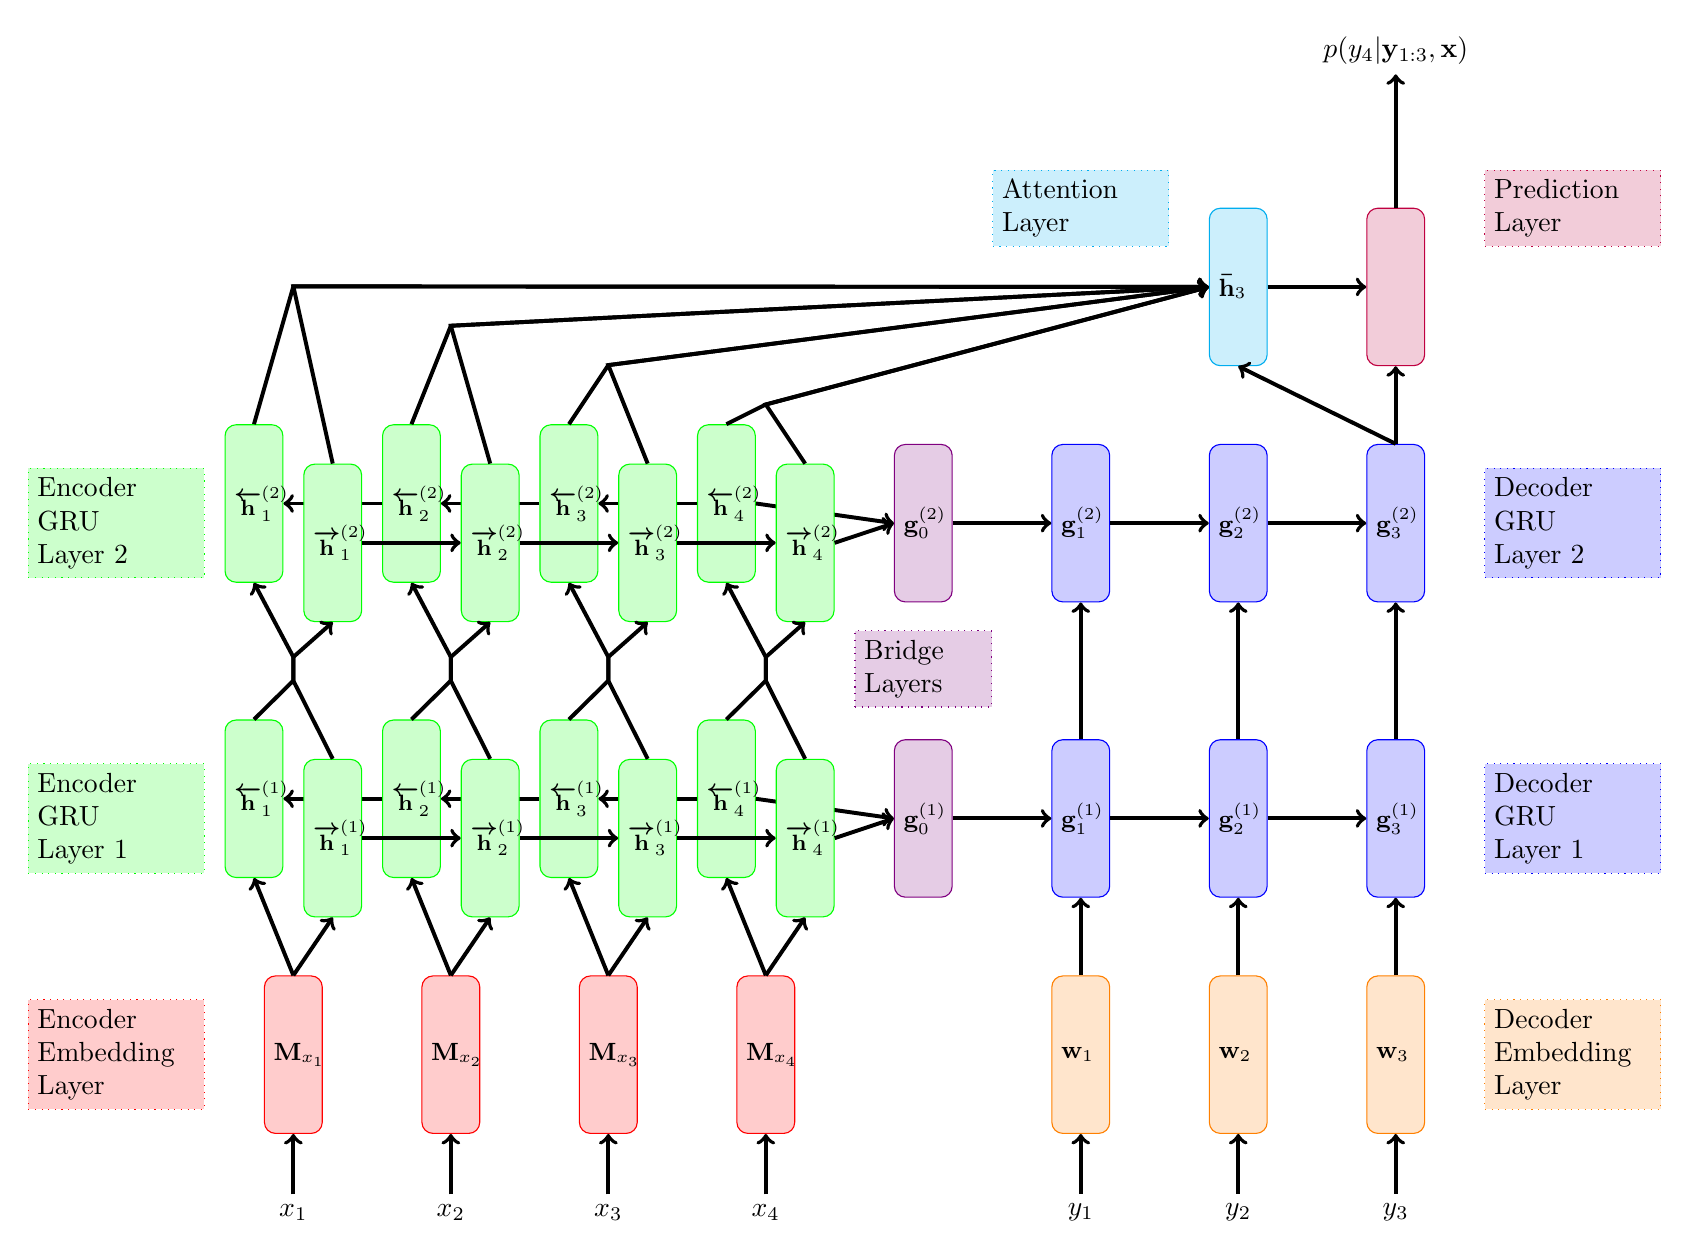
\begin{tikzpicture}[
    dhid/.style={draw,minimum height=2cm,fill=white,text width=5mm,font=\footnotesize,fill=green!20,draw=green,rounded corners},
    emb/.style={draw,minimum height=2cm,fill=white,text width=5mm,font=\small,rounded corners},
    emb.enc/.style={emb,fill=red!20,draw=red},
    emb.dech/.style={emb,fill=blue!20,draw=blue},
    emb.dec/.style={emb,fill=orange!20,draw=orange},
    emb.bridge/.style={emb,fill=violet!20,draw=violet},
    emb.attn/.style={emb,fill=cyan!20,draw=cyan},
    emb.pred/.style={emb,fill=purple!20,draw=purple},
    con/.style={line width=0.5mm}]

\node (x1) at (0,0) {$\mrtok_1$};
\node (x2) at (2,0) {$\mrtok_2$};
\node (x3) at (4,0) {$\mrtok_3$};
\node (x4) at (6,0) {$\mrtok_4$};

\node[emb.enc] (m1) at ($(x1)+(0,2)$) {$\encEmbs_{\mrtok_1}$};
\node[emb.enc] (m2) at ($(x2)+(0,2)$) {$\encEmbs_{\mrtok_2}$};
\node[emb.enc] (m3) at ($(x3)+(0,2)$) {$\encEmbs_{\mrtok_3}$};
\node[emb.enc] (m4) at ($(x4)+(0,2)$) {$\encEmbs_{\mrtok_4}$};

\draw[con,->] (x1.north) -- (m1.south);
\draw[con,->] (x2.north) -- (m2.south);
\draw[con,->] (x3.north) -- (m3.south);
\draw[con,->] (x4.north) -- (m4.south);

\node[draw=red,dotted,fill=red!20,text width=2cm,align=left] at ($(m1)+(-2.25,0)$) {Encoder\\ Embedding\\ Layer};

\node[draw=green,dotted,fill=green!20,text width=2cm,align=left] at ($(m1)+(-2.25,6.75)$) {Encoder\\ GRU\\ Layer 2};

\node[draw=green,dotted,fill=green!20,text width=2cm,align=left] at ($(m1)+(-2.25,3)$) {Encoder\\ GRU\\ Layer 1};

\node[emb.bridge] (g10) at ($(m4)+(2,3)$) {$\decHidState^{(1)}_0$};
\node[emb.bridge] (g20) at ($(m4)+(2,6.75)$) {$\decHidState^{(2)}_0$};

\node[draw=violet,dotted,fill=violet!20,text width=1.5cm,align=left] at (8,6.9) {Bridge\\ Layers};


\node (y1) at (10,0) {$\utttok_1$};
\node (y2) at (12,0) {$\utttok_2$};
\node (y3) at (14,0) {$\utttok_3$};

\node[emb.dec] (w1) at ($(y1)+(0,2)$) {$\decWordEmb_1$};
\node[emb.dec] (w2) at ($(y2)+(0,2)$) {$\decWordEmb_2$};
\node[emb.dec] (w3) at ($(y3)+(0,2)$) {$\decWordEmb_3$};

\node[draw=orange,dotted,fill=orange!20,text width=2cm,align=left] at ($(w3)+(2.25,0)$) {Decoder\\ Embedding\\ Layer};

\draw[con,->] (y1.north) -- (w1.south);
\draw[con,->] (y2.north) -- (w2.south);
\draw[con,->] (y3.north) -- (w3.south);

\node[emb.dech] (g11) at ($(w1)+(0,3)$) {$\decHidState^{(1)}_1$};
\node[emb.dech] (g12) at ($(w2)+(0,3)$) {$\decHidState^{(1)}_2$};
\node[emb.dech] (g13) at ($(w3)+(0,3)$) {$\decHidState^{(1)}_3$};

\node[emb.dech] (g21) at ($(w1)+(0,6.75)$) {$\decHidState^{(2)}_1$};
\node[emb.dech] (g22) at ($(w2)+(0,6.75)$) {$\decHidState^{(2)}_2$};
\node[emb.dech] (g23) at ($(w3)+(0,6.75)$) {$\decHidState^{(2)}_3$};


\node[dhid] (rh11) at ($(m1)+(-0.5,3+.25)$) {$\encBwdHidState^{(1)}_1$};
\node[dhid] (rh12) at ($(m2)+(-0.5,3+.25)$) {$\encBwdHidState^{(1)}_2$};
\node[dhid] (rh13) at ($(m3)+(-0.5,3+.25)$) {$\encBwdHidState^{(1)}_3$};
\node[dhid] (rh14) at ($(m4)+(-0.5,3+.25)$) {$\encBwdHidState^{(1)}_4$};
\draw[con,->] (rh14.west) -- (rh13.east);
\draw[con,->] (rh13.west) -- (rh12.east);
\draw[con,->] (rh12.west) -- (rh11.east);
\draw[con,->] (rh14.east) -- (g10.west);




\node[dhid] (fh11) at ($(m1)+(0.5,3-.25)$) {$\encFwdHidState^{(1)}_1$};
\node[dhid] (fh12) at ($(m2)+(0.5,3-.25)$) {$\encFwdHidState^{(1)}_2$};
\node[dhid] (fh13) at ($(m3)+(0.5,3-.25)$) {$\encFwdHidState^{(1)}_3$};
\node[dhid] (fh14) at ($(m4)+(0.5,3-.25)$) {$\encFwdHidState^{(1)}_4$};


\draw[con,->] (fh11.east) -- (fh12.west);
\draw[con,->] (fh12.east) -- (fh13.west);
\draw[con,->] (fh13.east) -- (fh14.west);
\draw[con,->] (fh14.east) -- (g10.west);

\node[dhid] (rh21) at ($(m1)+(-0.5,2.25*3+.25)$) {$\encBwdHidState^{(2)}_1$};
\node[dhid] (rh22) at ($(m2)+(-0.5,2.25*3+.25)$) {$\encBwdHidState^{(2)}_2$};
\node[dhid] (rh23) at ($(m3)+(-0.5,2.25*3+.25)$) {$\encBwdHidState^{(2)}_3$};
\node[dhid] (rh24) at ($(m4)+(-0.5,2.25*3+.25)$) {$\encBwdHidState^{(2)}_4$};
\draw[con,->] (rh24.west) -- (rh23.east);
\draw[con,->] (rh23.west) -- (rh22.east);
\draw[con,->] (rh22.west) -- (rh21.east);
\draw[con,->] (rh24.east) -- (g20.west);




\node[dhid] (fh21) at ($(m1)+(0.5,2.25*3-.25)$) {$\encFwdHidState^{(2)}_1$};
\node[dhid] (fh22) at ($(m2)+(0.5,2.25*3-.25)$) {$\encFwdHidState^{(2)}_2$};
\node[dhid] (fh23) at ($(m3)+(0.5,2.25*3-.25)$) {$\encFwdHidState^{(2)}_3$};
\node[dhid] (fh24) at ($(m4)+(0.5,2.25*3-.25)$) {$\encFwdHidState^{(2)}_4$};


\draw[con,->] (fh21.east) -- (fh22.west);
\draw[con,->] (fh22.east) -- (fh23.west);
\draw[con,->] (fh23.east) -- (fh24.west);
\draw[con,->] (fh24.east) -- (g20.west);



\draw[con,->] (m1.north) -- (fh11.south);
\draw[con,->] (m2.north) -- (fh12.south);
\draw[con,->] (m3.north) -- (fh13.south);
\draw[con,->] (m4.north) -- (fh14.south);
\draw[con,->] (m1.north) -- (rh11.south);
\draw[con,->] (m2.north) -- (rh12.south);
\draw[con,->] (m3.north) -- (rh13.south);
\draw[con,->] (m4.north) -- (rh14.south);

\foreach \i in {1,...,4} {
    \draw[con,->] (fh1\i.north) -- ($(fh1\i)!0.5!(rh1\i)+(0,1.75)$) -- 
        ($(fh1\i)!0.5!(rh1\i)+(0,2.05)$) -- (fh2\i.south);

    \draw[con,->] (rh1\i.north) -- ($(fh1\i)!0.5!(rh1\i)+(0,1.75)$) -- 
        ($(fh1\i)!0.5!(rh1\i)+(0,2.05)$) -- (rh2\i.south);
}


\draw[con,->] (g10) -- (g11);
\draw[con,->] (g20) -- (g21);
\draw[con,->] (w1) -- (g11);
\draw[con,->] (w2) -- (g12);
\draw[con,->] (w3) -- (g13);
\draw[con,->] (g11) -- (g21);
\draw[con,->] (g12) -- (g22);
\draw[con,->] (g13) -- (g23);
\draw[con,->] (g11) -- (g12);
\draw[con,->] (g12) -- (g13);
\draw[con,->] (g21) -- (g22);
\draw[con,->] (g22) -- (g23);

\node[emb.attn] (attn) at ($(g22)+(0,3)$) {$\astate_3$};


\draw[con,->] (rh21.north) -- ($(rh21.north)!0.5!(fh21.north)+(0,2.0)$) 
    -- (attn.west);
\draw[con,->] (fh21.north) -- ($(rh21.north)!0.5!(fh21.north)+(0,2.0)$) 
    -- (attn.west);

\draw[con,->] (rh22.north) -- ($(rh22.north)!0.5!(fh22.north)+(0,1.5)$) 
    -- (attn.west);
\draw[con,->] (fh22.north) -- ($(rh22.north)!0.5!(fh22.north)+(0,1.5)$) 
    -- (attn.west);

\draw[con,->] (rh23.north) -- ($(rh23.north)!0.5!(fh23.north)+(0,1.0)$) 
    -- (attn.west);
\draw[con,->] (fh23.north) -- ($(rh23.north)!0.5!(fh23.north)+(0,1.0)$) 
    -- (attn.west);

\draw[con,->] (rh24.north) -- ($(rh24.north)!0.5!(fh24.north)+(0,0.5)$) 
    -- (attn.west);
\draw[con,->] (fh24.north) -- ($(rh24.north)!0.5!(fh24.north)+(0,0.5)$) 
    -- (attn.west);

\draw[con,->] (g23.north) -- (attn.south);

\node[emb.pred] (z) at ($(g23)+(0,3)$) {\phantom{$z_3$}};

\node (p) at ($(z)+(0,3)$) {$\gen(\utttok_4|\utttoks_{1:3},\mrtoks)$};
\draw[con,->] (z.north) -- (p.south);
\draw[con,->] (g23.north) -- (z.south);
\draw[con,->] (attn.east) -- (z.west);

\node[draw=blue,dotted,fill=blue!20,text width=2cm,align=left] at ($(w3)+(2.25,3)$) {Decoder\\ GRU\\ Layer 1};
\node[draw=blue,dotted,fill=blue!20,text width=2cm,align=left] at ($(w3)+(2.25,6.75)$) {Decoder\\ GRU\\ Layer 2};


\node[draw=cyan,dotted,fill=cyan!20,text width=2cm,align=left] at ($(attn)+(-2,1)$) {Attention\\ Layer};
\node[draw=purple,dotted,fill=purple!20,text width=2cm,align=left] at ($(z)+(2.25,1)$) {Prediction\\ Layer};
\end{tikzpicture}
}
\caption{Schematic of the bi-directional GRU-based \sequencetosequence~model.}
\label{fig:s2s}
\end{figure}


The GRU is a form of reccurent neural network \citep{elman1990} that operates
over discrete sequences, which upon receiving a new input token, updates a
``hidden state'' or internal representation using the current input and the
previous hidden state. In the \sequencetosequence~paradigm, both the encoder
and decoder are built upon distinct GRU layers. 

The encoder consists of an embedding layer which maps the discrete input
sequence to a sequence embeddings. The encoder input embedding sequence is
then fed through one or more GRU layers. Optionally, the encoder GRUs can be
run uni-directionally (i.e., proceeding left-to-right), or bi-directionally
(i.e. distinct left-to-right and right-to-left GRUs process the input sequence
and concatenate the output). We describe both cases below. After encoding the
input, the final state of the encoder is optionally run through a bridge layer
to project it to a compatible size for the decoder. 

The decoder also has an embedding layer which it uses to map previously
generated output tokens to embeddings which are then fed into the one or more
uni-directional decoder GRUs. The decoder hidden state at each step attends to
the encoder hidden states, producing an ``attention vector,'' i.e. a weighted
sum of the encoder hidden states. The decoder state and the attention vector
are concatenated and fed through a \feedforward~layer with softmax output to
produce a probability distribution over the next token. 

See \autoref{fig:s2s} for a schematic example of the GRU-based
\sequencetosequence~model. We now describe the individual components in
detail.

\paragraph{\redbox{Encoder Embedding Layer}}
Let $\mrtoks = \left[ \mrtok_1,\ldots,\mrtok_\mrSize\right]$ be a linearized
\meaningrepresentation~token sequence. Before feeding $\mrtoks$ into the
encoder GRU layer, we first embed each token. Let $\encEmbs \in
\reals^{\setsize{\mrvocab} \times \embDim}$ be the encoder input embedding
matrix, where each row, $\encWordEmb_i$, is a $\embDim$-dimensional embedding
for a token in $\utttok \in \mrvocab$, i.e.,
\[ 
    \encEmbs = \left[ \begin{array}{c} \encWordEmb_1\\ \vdots \\ \encWordEmb_\setsize{\mrvocab} \end{array}\right]. 
\]
We assume each element $\mrtok \in \mrvocab$ is uniquely identified with a row
$i \in \left\{1, \ldots, \setsize{\mrvocab}\right\}$. We indicate the
embedding of $\mrtok$ as $\encEmbs_\mrtok = \encWordEmb_i$.  The input to the
encoder GRU layer then is 
\[
\left[\encHidState^{(0)}_1,\ldots,\encHidState^{(0)}_\mrSize\right] = 
    \left[\encEmbs_{\mrtok_1},\ldots,   \encEmbs_{\mrtok_\mrSize}\right]. 
\]


\paragraph{\greenbox{Encoder Uni-directional GRU Layers}}
We then compute the GRU hidden states. The encoder can have an arbitray number of layers $\numLayer$.
For each layer $l \in \{1,\ldots, \numLayer\}$ we compute,
\begin{align*}
    \encHidState_0^{(l)} & = \zeroEmb \\
    \encHidState_i^{(l)} & =\fgru(\encHidState_i^{(l - 1)}, \encHidState_{i-1}^{(l)}; \gruEncParams^{(l)}) & \forall i : i \in \{1,\ldots, \mrSize\}
\end{align*}
where $\gruEncParams^{(l)}$ are the GRU encoder parameters\footnote{See \autoref{eqn:gru} for the definition of the GRU function.} for the $l$-th layer and $\encHidState^{(l)}_i \in \reals^{\hidDim}$. The encoder GRU layers output the 
sequence of hidden states, $\encHidState_1,\ldots,\encHidState_\mrSize$, used by the decoder to represent the input; 
in the uni-directional case, these are simply the last GRU layer outputs, i.e. $\encHidState_i = \encHidState_i^{(\numLayer)} \in \reals^{\encDim}$ (in the uni-directional case, $\hidDim = \encDim$).

\paragraph{\greenbox{Encoder Bi-directional GRU Layers}}
The uni-directional encoder may suffer from a recency bias when creating the initial state for the 
decoder and for longer input sequences the encoder may ``forget'' information encoded in the 
early hidden states. In practice to alleviate this another GRU is run in the opposite direction and
its outputs are concatenated. For the first layer, we have,
\begin{align*}
    \textit{(Encoder Forward GRU)}\\
    \encFwdHidState_0^{(1)} & = \zeroEmb,\\ 
    \encFwdHidState_i^{(1)} & =\fgru\left(\encHidState_i^{(0)}, \encFwdHidState_{i-1}^{(1)}; \gruEncFwdParams^{(l)}\right), & \forall i : i \in \{1,\ldots, \mrSize\}\\
    \textit{(Encoder Backward GRU)}\\
     \encBwdHidState_0^{(1)} &= \zeroEmb, \\
    \encBwdHidState_i^{(1)} & =\fgru\left(\encHidState_i^{(0)}, \encBwdHidState_{i+1}^{(1)}; \gruEncBwdParams^{(l)}\right)    & \forall i : i \in \{1,\ldots, \mrSize\}\\
  \encHidState^{(1)}_i & = \left[\begin{array}{c} \encFwdHidState_i^{(1)} \\ \encBwdHidState_i^{(1)} \end{array}\right]
& \forall i : i \in \{1,\ldots, \mrSize\}\\
\end{align*}
where $\gruEncFwdParams$ and $\gruEncBwdParams$ are forward and backward GRU parameters respectively,
$\encFwdHidState^{(1)}_i,\encBwdHidState^{(1)}_i\in\reals^{\hidDim}$, and first layer hidden state,
$\encHidState^{(1)}_i\in\reals^{2\hidDim}$, is a concatenation of the forward and backward hidden
states at step $i$. 
The subsequent layers are computed similarly, but the input to the GRUs are $2\hidDim$-dimensional.
Like before, the encoder outputs are the hidden state outputs of the last layer, $\encHidState_i = \encHidState_i^{(\numLayer)} \in \reals^{\encDim}$ where $\encDim = 2\hidDim$.


\paragraph{\orangebox{Decoder Embedding Layer}}
We then embed the utterance token sequence, 
$\utttoks = \left[ \utttok_1,\ldots,\utttok_\uttSize\right]$,
before feeding it to the decoder GRU layers.. 
Let $\decEmbs \in \reals^{\setsize{\uttvocab} \times \embDim}$ be an
embedding matrix of the utterance tokens $\utttok \in \uttvocab$ defined
analogously to the encoder embedding matrix $\encEmbs$. 
%where each row is an embedding for a token in $\uttvocab$ (analogous to $\encEmbs$),
%\[ \decEmbs = \left[ \begin{array}{c} \decWordEmb_1\\ \vdots \\ \decWordEmb_\setsize{\uttvocab} \end{array}\right]. \]
%We assume each element in $\uttvocab$ is uniquely identified with a row in $\encEmbs$; let $\mrtok\in\mrvocab$ be identified with the $i$-th row, then we indicate it's embedding by $\encEmbs_\mrtok = \encWordEmb_i$.  
The input to the decoder then is 
\[\left[\decHidState^{(0)}_1,\ldots,\decHidState^{(0)}_{\uttSize-1}\right] = \left[\decEmbs_{\utttok_1},\ldots,
\decEmbs_{\utttok_{\uttSize-1}}\right].\footnote{The decoder input sequences have length $\uttSize-1$ since the $\uttSize^\textrm{th}$ token is always the stop token \stoptok, which is never fed into the decoder input. } \]

\paragraph{\violetbox{Bridge Layer}}
We initialize the decoder hidden state with the final (i.e. $\mrSize$-th) state of the encoder GRU.
In the case where $\encDim \ne \hidDim$, we need to project $\encHidState_\mrSize^{(l)}$ to $\hidDim$
dimensions,
\[ \decHidState_0^{(l)} = \begin{cases} \tanh\left(\weight{br}_l \encHidState_\mrSize^{(l)} + \bias{br}_l\right) & \encDim \ne \hidDim  \\
\encHidState_\mrSize^{(l)} & \textrm{otherwise} \end{cases},\]
where $\weight{br}_l \in \reals^{\hidDim \times \encDim}$ and $\bias{br}_l \in \reals^{\hidDim}$
for $l \in \{1,\ldots,\numLayer\}$
are the weight and bias parameters for the ``bridge layer'' between the encoder and decoder networks.

\paragraph{\bluebox{Decoder GRU Layers}}
The decoder GRU is then computed analogously to the uni-directional encoder GRU,
\begin{align*}
    \decHidState_i^{(l)} & =\fgru\left(\decHidState_i^{(l - 1)}, \decHidState_{i-1}^{(l)}; \gruDecParams^{(l)}\right) & \forall i : i \in \{1,\ldots, \uttSize-1\},
\end{align*}
where $\gruDecParams^{(l)}$ are the decoder GRU parameters and
$ \decHidState_i^{(l)} \in \reals^{\hidDim}$ for $i \in \{1,\ldots,\uttSize-1\}$ and $l \in \{1,\ldots,\numLayer\}$.
The decoder outputs, $\decHidState_1,\ldots,\decHidState_{\uttSize-1}$, are the decoder hidden states of the last decoder layer, i.e. $\decHidState_i = \decHidState^{(\numLayer)}_i \in \reals^{\decDim}$ where $\decDim=\hidDim$.

\paragraph{\cyanbox{Attention Layer}}

As mentioned before, one drawback of the recurrent neural network design is that information
from earlier states my not be preserved in later states. To ameliorate this, the attention
mechanism was proposed to allow an arbitrary decoder state to retrieve information from an arbitrary
encoder state \citep{bahdanau2015}. This works by taking a weighted average of the encoder states,
\begin{align*}
    \astate_i & = \sum^{\mrSize}_{j=1}\alpha_{i,j}\encHidState_j & \forall i : i \in \{1,\ldots, \uttSize-1\}
\end{align*}
where $\alpha_{i,j} \in (0,1)$ is proportional to a score function $\ascore(\decHidState_i,\encHidState_j)$ which 
measures some notion of ``relevance'' for decoder state $i$ to encoder start $j$,
\[\alpha_{i,j} = \frac{\exp \ascore(\decHidState_i, \encHidState_j) }{ \sum_{j^\prime=1}^\mrSize \exp \ascore(\decHidState_i, \encHidState_{j^\prime})} \quad \forall i,j : j \in \{1,\ldots,\mrSize\}, i \in \{1,\ldots,\uttSize-1\}.\]

There are several popular ways to implement $\ascore$ which we consider; we refer to three of them
using the names given in \citet{luong2015}. When the encoder and decoder
hidden states are of the same dimension, the simplest function is just the dot product, which 
we refer to as ``dot-style'' attention,\\
\textit{(Dot-Style Attention)}
\[ \quad \ascore(\decHidState_i,\encHidState_j) = \decHidState_i \cdot \encHidState_j. \]
If they are not the same dimension, one can insert a parameter matrix in place of the dot product,\\
\textit{(General-Style Attention)}
\[ \quad \ascore(\decHidState_i,\encHidState_j) = \decHidState_i \attnkernel \encHidState_j \]
where $\attnkernel \in \reals^{\decDim \times \encDim}$ is a learned parameter of the model.

The third method called ``concat'' by \citet{luong2015} but also commonly
referred to as ``Bahdanau,'' since it was introduced in the 
\citet{bahdanau2015}, uses a \feedforward~layer to project the pair of states
down to a scalar,\\
\textit{(Concat-Style Attention)}
\[ \ascore(\decHidState_i, \encHidState_j) = \attnff\cdot\tanh\left(\attnkernel\left[ \begin{array}{c} \decHidState_i \\ \encHidState_j \end{array} \right] \right),  \]
    where $\attnkernel \in \reals^{\hidDim \times (\decDim + \encDim)}$
    and $\attnff \in \reals^{\hidDim}$ are learned parameters.



\paragraph{\purplebox{Prediction Layer}}
Finally, the attention output $\astate_i$ and decoder state $\decHidState_i$
are run through a two~layer \feedforward~network to produce a distribution
over the utterance token vocabulary $\uttvocab$,
\[ \gen\left(\utttok_{i+1}|\utttoks_{1:i},\ls(\mr);\params\right) = \softmax\left(   \weight{2}\cdot \tanh\left(\weight{1} \left[ \begin{array}{c}\decHidState_i \\ \encHidState_j \end{array} \right] + \bias{1}\right) + \bias{2} \right)_{\utttok_{i+1}}\quad \forall i: i \in \{1,\ldots,\uttSize-1\} \]
    where $\weight{1} \in \reals^{\hidDim \times \left(\decDim + \encDim\right)}$,
    $\bias{1} \in \reals^{\hidDim}$, $\weight{2} \in \reals^{\setsize{\uttvocab} \times \hidDim}$, and $\bias{2}\in\reals^{\setsize{\uttvocab}}$ are learned
    parameters and we associate each utterance token $\utttok$ with a unique 
    element in the final $\softmax$ distribution (similar to how we indexed
    into the embeddings matrices $\encEmbs$ and $\decEmbs$). 



%    The complete set parameters associated with the GRU architecture 
%    with uni-directional encoder is
%    \[ \params = \left\{ \gruEncParams^{(1)},
%    \ldots, \gruEncParams^{(\numLayer)}, 
%    \weight{1}, \bias{1}, \weight{2}, \bias{2}
%    \right\}  \]
%    while the GRU
%    with bi-directional encoder parameters are
%    \[ \params = \left\{ \gruEncFwdParams^{(1)}, \gruEncBwdParams^{(1)},
%            \weight{br}_1, \bias{br}_1,
%    \ldots, \gruEncFwdParams^{(\numLayer)}, \gruEncBwdParams^{(\numLayer)},
%    \weight{br}_\numLayer, \bias{br}_\numLayer, \weight{1}, \bias{1}, \weight{2}, \bias{2}
%    \right\}  \]
%    TODO add attention params.
% 


\chapter{Transformer-based Sequence-to-Sequence Architecture}
\label{sec:nlgtf}

\begin{figure}[p]
\resizebox{\textwidth}{!}{
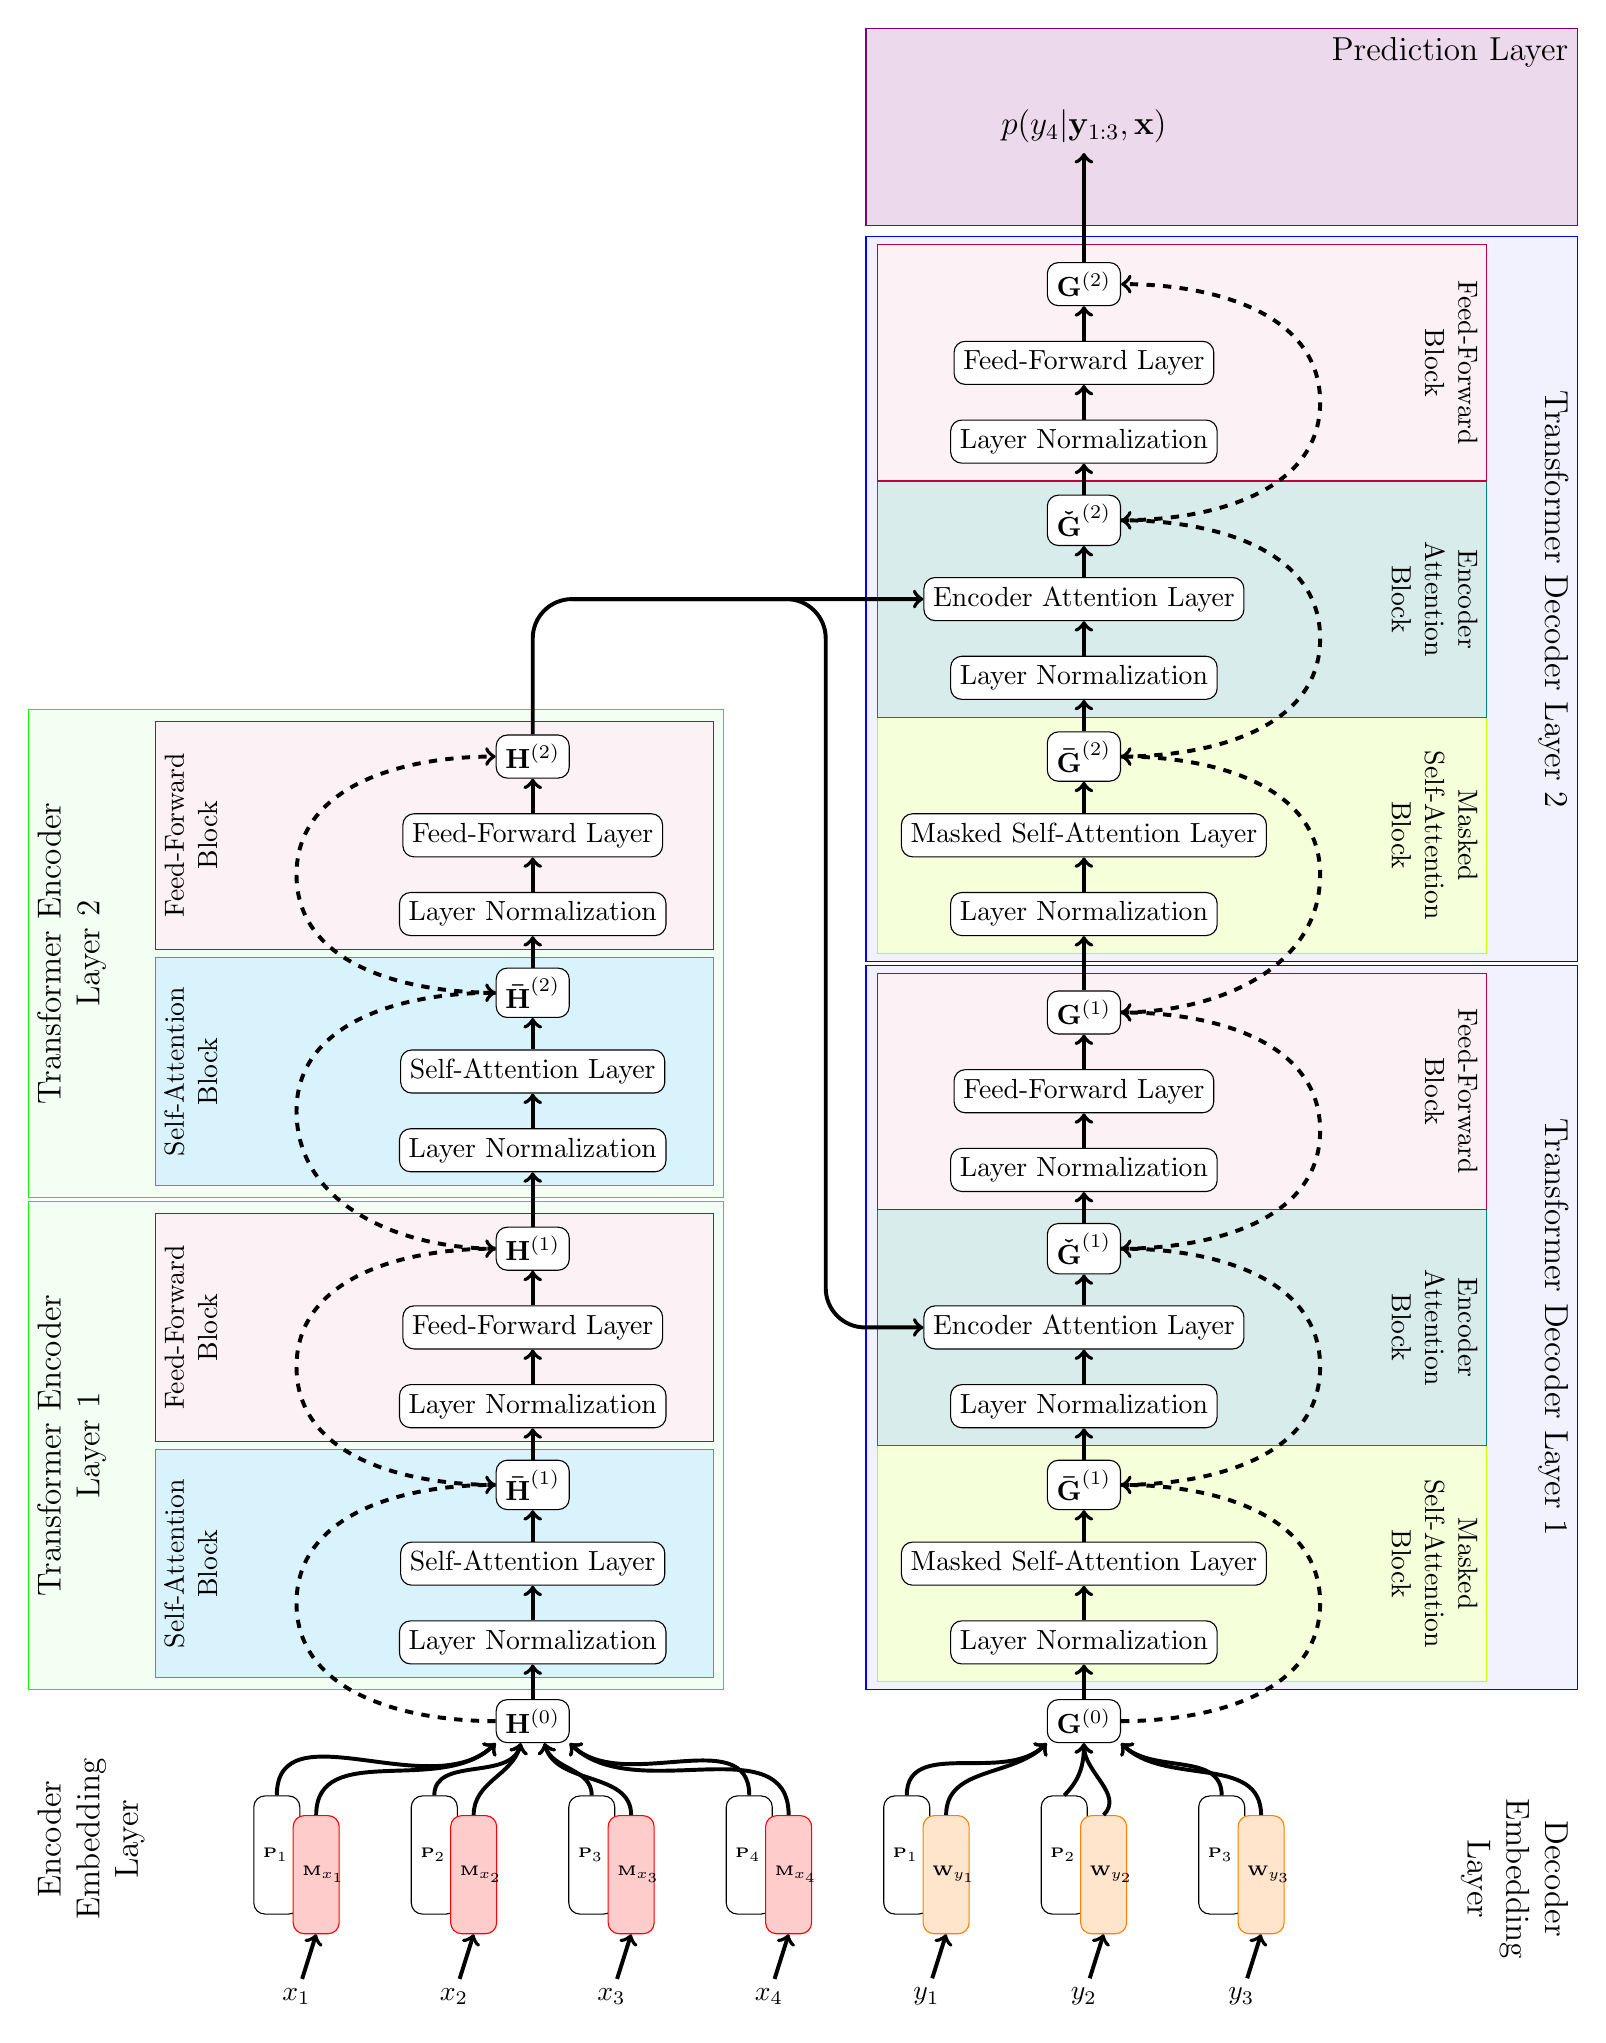
\begin{tikzpicture}[
    emb/.style={draw,minimum height=1.5cm,fill=white,text width=3.5mm,font=\tiny,rounded corners},
    emb.enc/.style={emb,fill=red!20,draw=red},
    emb.dec/.style={emb,fill=orange!20,draw=orange},
    penc/.style={emb,fill=white,draw=black},
    con/.style={line width=0.5mm},
    state/.style={draw,rounded corners,fill=white},
    ln/.style={state},
    selfattn/.style={state},
    encattn/.style={state},
    ff/.style={state},
    enclayer/.style={draw=green,text width=8.6cm,minimum height=6.2cm,
                     fill=green!5},
    declayer/.style={draw=blue,text width=8.8cm,minimum height=9.2cm,
                     fill=blue!5},
    ]

    \def\encbsz{6.25};
    \def\decbsz{9.25};

    \node[state] (H0) at (3,-1) {$\tfEncInput^{(0)}$};
    \foreach \i [count=\j from 1] in {0,...,1} {
        \node[enclayer] (enclayer\j) at (1.01,\i*\encbsz+2.5) {};
            \node[rotate=90,anchor=north,font=\large,align=center] at (enclayer\j.west) {Transformer Encoder\\ Layer \j};

        \node[draw,text width=6.85cm,minimum height=2.9cm,draw=cyan,fill=cyan!15] 
            (HA{\j}Block) at (3-1.25,\i*\encbsz+1) {};
        \node[anchor=north,rotate=90,align=center] 
            at (HA{\j}Block.west) {Self-Attention\\ Block};

        \node[draw,text width=6.85cm,minimum height=2.9cm,draw=purple,fill=purple!5] 
            (HFF{\j}Block) at (3-1.25,\i*\encbsz+4) {};
        \node[anchor=north,rotate=90,align=center] 
            at (HFF{\j}Block.west) {Feed-Forward\\ Block};

        \node[ln] (HLN\j1) at (3,\i*\encbsz+0) {Layer Normalization};
        \node[selfattn] (HA\j) at (3,\i*\encbsz+1) {Self-Attention Layer};
        \node[state] (H{\i}a) at (3,\i*\encbsz+2) 
            {$\boldsymbol{\bar{\tfEncInput}}^{(\j)}$};

        \node[ln] (HLN\j2) at (3,\i*\encbsz+3) {Layer Normalization};
        \node[ff] (HFF\j) at (3,\i*\encbsz+4) {Feed-Forward Layer};
        \node[state] (H\j) at (3,\i*\encbsz+5) 
            {$\tfEncInput^{(\j)}$};

        \draw[con,dashed,->] (H\i) to [out=180,in=270] ($(HLN\j1)!0.5!(HA\j)+(-3,0)$)
            to [out=90,in=180] (H{\i}a);
        \draw[con,dashed,->] (H{\i}a) to [out=180,in=270] ($(HLN\j2)!0.5!(HFF\j)+(-3,0)$)
            to [out=90,in=180] (H\j);
            
        \draw[con,->] (H\i) -- (HLN\j1);
        \draw[con,->] (HLN\j1) -- (HA\j);
        \draw[con,->] (HA\j) -- (H{\i}a);
        \draw[con,->] (H{\i}a) -- (HLN\j2);
        \draw[con,->] (HLN\j2) -- (HFF\j);
        \draw[con,->] (HFF\j) -- (H\j);


    }


    \node[state] (G0) at (10,-1) {$\tfDecInput^{(0)}$};
    \foreach \i [count=\j from 1] in {0,...,1} {
    
        \node[declayer] (declayer\j) at (11.75,\i*\decbsz+4) {};
        \node[rotate=-90,anchor=north,font=\large] at (declayer\j.east) {Transformer Decoder Layer \j};

        \node[draw=lime,fill=lime!15,text width=7.50cm,minimum height=3cm] 
            (GA{\j}Block) at (10+1.25,\i*\decbsz+1) {};
        \node[anchor=north,rotate=-90,align=center] 
            at (GA{\j}Block.east) {Masked \\ Self-Attention\\ Block};
 
        \node[draw=teal,text width=7.50cm,minimum height=3cm,fill=teal!15] 
            (GEA{\j}Block) at (10+1.25,\i*\decbsz+4) {};
        \node[anchor=north,rotate=-90,align=center] 
            at (GEA{\j}Block.east) {Encoder\\Attention\\ Block};
 
        \node[draw=purple,fill=purple!5,text width=7.50cm,minimum height=3cm] 
            (GFF{\j}Block) at (10+1.25,\i*\decbsz+7) {};
        \node[anchor=north,rotate=-90,align=center] 
            at (GFF{\j}Block.east) {Feed-Forward\\ Block};
        
        \node[ln] (GLN\j1) at (10,\i*\decbsz+0) {Layer Normalization};
        \node[selfattn] (GA\j) at (10,\i*\decbsz+1) {Masked Self-Attention Layer};
        \node[state] (G{\i}a) at (10,\i*\decbsz+2) 
            {$\boldsymbol{\bar{\tfDecInput}}^{(\j)}$};

        \node[ln] (GLN\j2) at (10,\i*\decbsz+3) {Layer Normalization};
        \node[encattn] (GEA\j) at (10,\i*\decbsz+4) {Encoder Attention Layer};
        \node[state] (G{\i}b) at (10,\i*\decbsz+5) 
            {$\boldsymbol{\check{\tfDecInput}}^{(\j)}$};

        \node[ln] (GLN\j3) at (10,\i*\decbsz+6) {Layer Normalization};
        \node[ff] (GFF\j) at (10,\i*\decbsz+7) {Feed-Forward Layer};
        \node[state] (G\j) at (10,\i*\decbsz+8) {$\tfDecInput^{(\j)}$};

        \draw[con,->,dashed] (G\i) to [out=0,in=270] ($(GLN\j1)!0.5!(GA\j)+(3,0)$)
            to [out=90,in=0] (G{\i}a);
        \draw[con,->,dashed] (G{\i}a) to [out=0,in=270] ($(GLN\j2)!0.5!(GEA\j)+(3,0)$)
            to [out=90,in=0] (G{\i}b);
        \draw[con,->,dashed] (G{\i}b) to [out=0,in=270] ($(GLN\j3)!0.5!(GFF\j)+(3,0)$)
            to [out=90,in=0] (G\j);
        \draw[con,->] (G\i) -- (GLN\j1);
        \draw[con,->] (GLN\j1) -- (GA\j);
        \draw[con,->] (GA\j) -- (G{\i}a);
        \draw[con,->] (G{\i}a) -- (GLN\j2);
        \draw[con,->] (GLN\j2) -- (GEA\j);
        \draw[con,->] (GEA\j) -- (G{\i}b);
        \draw[con,->] (G{\i}b) -- (GLN\j3);
        \draw[con,->] (GLN\j3) -- (GFF\j);
        \draw[con,->] (GFF\j) -- (G\j);

    }


    \node (x1) at (0,-4.5) {$\mrtok_1$};
    \node (x2) at (2,-4.5) {$\mrtok_2$};
    \node (x3) at (4,-4.5) {$\mrtok_3$};
    \node (x4) at (6,-4.5) {$\mrtok_4$};
    \node (y1) at (8,-4.5) {$\utttok_1$};
    \node (y2) at (10,-4.5) {$\utttok_2$};
    \node (y3) at (12,-4.5) {$\utttok_3$};

    \node[declayer,minimum height=2.5cm,draw=violet,fill=violet!15] (predlayer) at (11.75,1*\decbsz+10) {};
    \node[font=\large] (prob) at ($(G2)+(0,2)$) {$\gen(\utttok_4|\utttoks_{1:3}, \mrtoks)$};

    \node[anchor=north east,font=\large]  at ($(predlayer.north east)$) {Prediction Layer};
    %\node[font=\large]  at ($(G2)+(-4,2)$) {Prediction Layer};



    \draw[con,->] (G2.north) -- (prob.south);

    \node[penc] (pe1) at ($(x1)+(-0.25,2-.2)$) {$\posEmb_1$};
    \node[penc] (pe2) at ($(x2)+(-0.25,2-.2)$) {$\posEmb_2$};
    \node[penc] (pe3) at ($(x3)+(-0.25,2-.2)$) {$\posEmb_3$};
    \node[penc] (pe4) at ($(x4)+(-0.25,2-.2)$) {$\posEmb_4$};
    \node[emb.enc] (m1) at ($(x1)+(0.25,1.75-.2)$) {$\encEmbs_{\mrtok_1}$};
    \node[emb.enc] (m2) at ($(x2)+(0.25,1.75-.2)$) {$\encEmbs_{\mrtok_2}$};
    \node[emb.enc] (m3) at ($(x3)+(0.25,1.75-.2)$) {$\encEmbs_{\mrtok_3}$};
    \node[emb.enc] (m4) at ($(x4)+(0.25,1.75-.2)$) {$\encEmbs_{\mrtok_4}$};

    \draw[con,->] (m1.north) to [out=90,in=225] (H0.south west);
    \draw[con,->] (pe1.north) to [out=90,in=225] (H0.south west);

    \draw[con,->] (m2.north) to [out=90,in=255] ($(H0.south)+(-.15,0)$);
    \draw[con,->] (pe2.north) to [out=90,in=255] ($(H0.south)+(-.15,0)$);

    \draw[con,->] (m3.north) to [out=90,in=285]  ($(H0.south)+(.15,0)$);

    \draw[con,->] (pe3.north) to [out=90,in=285] ($(H0.south)+(.15,0)$);

    \draw[con,->] (m4.north) to [out=90,in=315] (H0.south east);
    \draw[con,->] (pe4.north) to [out=90,in=315] (H0.south east);

    \draw[con,->] (x1) -- (m1.south);
    \draw[con,->] (x2) -- (m2.south);
    \draw[con,->] (x3) -- (m3.south);
    \draw[con,->] (x4) -- (m4.south);

    \node[penc] (pd1) at ($(y1)+(-0.25,2-.2)$) {$\posEmb_1$};
    \node[penc] (pd2) at ($(y2)+(-0.25,2-.2)$) {$\posEmb_2$};
    \node[penc] (pd3) at ($(y3)+(-0.25,2-.2)$) {$\posEmb_3$};

    \node[emb.dec] (w1) at ($(y1)+(0.25,1.75-.2)$) {$\decEmbs_{\utttok_1}$};
    \node[emb.dec] (w2) at ($(y2)+(0.25,1.75-.2)$) {$\decEmbs_{\utttok_2}$};
    \node[emb.dec] (w3) at ($(y3)+(0.25,1.75-.2)$) {$\decEmbs_{\utttok_3}$};
    \draw[con,->] (w1.north) to [out=90,in=225] (G0.south west);
    \draw[con,->] (pd1.north) to [out=90,in=225] (G0.south west);

    \draw[con,->] (w2.north) to [out=45,in=270] (G0.south);
    \draw[con,->] (pd2.north) to [out=45,in=270] (G0.south);

    \draw[con,->] (w3.north) to [out=90,in=315]  (G0.south east);
    \draw[con,->] (pd3.north) to [out=90,in=315] (G0.south east);

    \draw[con,->] (y1) -- (w1.south);
    \draw[con,->] (y2) -- (w2.south);
    \draw[con,->] (y3) -- (w3.south);

    \node (z1) at (H2 |- GEA2) {};

    \node (z2) at ($(z1)!0.75!(GEA2.west)$) {};

    \node (z1s) at ($(z1)+(0,-0.5)$) {};
    \node (z1e) at ($(z1)+(0.5,0.0)$) {};
    
    \node (z2s) at ($(z2)+(0,-0.5)$) {};
    \node (z2w) at ($(z2)+(-0.5,0.0)$) {};
    \node (z3) at (z2 |- GEA1) {};

    \node (z3n) at ($(z3)+(0,0.5)$) {};
    \node (z3e) at ($(z3)+(0.5,0.0)$) {};

    \draw[con,->] (H2.north) -- (z1s.center) to [out=90,in=180] (z1e.center) -- (z2.center) -- (GEA2.west);
    \draw[con,->] (z1e.center) -- (z2w.center) to [out=0,in=90] (z2s.center) -- (z3n.center) to [out=270,in=180] (z3e.center) -- (GEA1.west);

    \node[rotate=90,anchor=north,align=center,font=\large] at ($(enclayer1.west)+(0,-5)$) {Encoder \\ Embedding\\ Layer};

    \node[rotate=-90,anchor=north,align=center,font=\large] at ($(declayer1.east)+(0,-7)$) {Decoder \\ Embedding\\ Layer};
\end{tikzpicture}
}
\caption{A schematic diagram of a two layer transformer-based \sequencetosequence~model. Dashed lines indicate skip-connections.}
\label{fig:tf}
\end{figure}


The transformer \sequencetosequence~model eschews the recurrence as a mechanism
for propagating information, and instead leans solely on several 
attention mechanisms to learn representations of the input sequence $\mrtoks$
as well as the decoder input prefix $\utttoks_{1:i}$. Like the GRU,
each encoder and decoder consist of $\numLayer$ distinct
layers which are applied to $\mrtoks$ and $\utttoks_{1:i}$ respectively.
Ultimately,
the decoder outputs are used to compute the next word probability,
$\gen(\utttok_{i+1}|\utttoks_{1:i},\mrtoks)$. 

A schematic diagram of the transformer-based \sequencetosequence~model
is shown in \autoref{fig:tf}. Like the GRU schematic, the model diagram is 
color-coded to correspond with the text descriptions of each component.
While the transformer looks significantly more complex than the 
GRU architecture, it is fundamentally built around only three 
different kinds of 
neural network layers, \textit{(i)} multi-head attention, 
\textit{(ii)} \feedforward layers, and \textit{(iii)} 
layer normalization. Before describing the encoder and decoder layers
in detail, we first describe these basic components and how they form 
the various ``block'' structures which are employed throughout the model.

\subsubsection{Transformer Components}

\paragraph{Multi-Head Attention} The first basic layer to be defined is the 
multi-head attention layer. We begin by describing ``single-head'' attention
from the point of view of a soft key-value store and then generalize to 
the ``multi-head'' case. In this view, we assume we want to attend to 
a sequence of $\mrSize$ items. Each item has two representations,
a key representation and a value representation, which are written collectively
as rows in a key and value matrix, $\Key \in \reals^{\mrSize \times \embDim}$
and $\Value \in \reals^{\mrSize \times \embDim}$ respectively.
We then  have $\uttSize$ query items that will each individually attend to the 
$\mrSize$ items; we similarly represent the query items as rows in a matrix
$\Query \in \reals^{\uttSize \times \embDim}$. An attention
layer, denoted $\Attn : \reals^{\uttSize \times \embDim} \times \reals^{\mrSize \times \embDim} \times \reals^{\mrSize \times \embDim} \rightarrow \reals^{\uttSize \times \embDim}$, then computes an attention weighted read of the value
matrix as,
  \[\Attn\left(\Query, \Key, \Value\right) = \softmax\left(\frac{\Query \Key^T}{\sqrt{\embDim}} \right)\Value, \]
  where \[\softmax\left(\frac{\Query \Key^T}{\sqrt{\embDim}} \right)_{i,j} = \frac{\exp\left(\embDim^{-\frac{1}{2}} \mathbf{q}_i \cdot \mathbf{k}_j\right) }{ \sum_{j^\prime=1}^\mrSize \exp\left( \embDim^{-\frac{1}{2}} \mathbf{q}_i \cdot \mathbf{k}_{j^\prime}\right)} \quad \forall i,j : i \in \{1,\ldots,\uttSize\}, j \in \{1,\ldots,\mrSize\}.\]
  Because the $\mrSize$ items have distinct key and value matrices,
  representation of similarity between a query and a key can be different
  than the value that is produced in the output, unlike the attention
  mechanisms discussed in the GRU decoder, where essentially, the key
  and values were identical representations.


  The idea behind multi-head attention is to compute $\numHeads$ distinct
  attention operations by first projecting the query, keys, and values
  down to a smaller representation. That is, given projection
  matrices, $\weight{Q_{in},k}, \weight{K_{in},k}, \weight{V_{in},k} \in \reals^{\embDim \times \frac{\embDim}{\numHeads}}$ for $k \in \{1,\ldots,\numHeads\}$, and $\weight{V_{out}} \in \reals^{\embDim \times \embDim}$,
the  multi-headed attention layer computes
\[ \MultiAttn(\Query, \Key, \Value) = \left(\begin{array}{lc}
            &\Attn\left(\Query\weight{Q_{in},1},  
                 \Key\weight{K_{in},1}, \Value\weight{V_{in},1}\right)\\
              \oplus &   
                  \Attn\left(\Query\weight{Q_{in},2}, 
              \Key\weight{K_{in},2}, \Value\weight{V_{in},2}\right)\\
              & \vdots \\
              \oplus & 
            \Attn\left(\Query\weight{Q_{in},\numHeads},  
                 \Key\weight{K_{in},\numHeads}, \Value\weight{V_{in},\numHeads}\right)\\
        \end{array}\right) \weight{V_{out}}
 \]
  where $\oplus$ indicates column-wise concatenation. Each use of a
  multi-head attention layer uses distinct projection matrices
  and are learned parameters of the model.

%~\\~\\
%
%the single-headed attention layer takes three matrices as input:
%a query matrix, $\Query \in \reals^{\uttSize \times \embDim}$,
%a key matrix, $\Key \in \reals^{\mrSize \times \embDim}$,
%and a value matrix, $\Value \in \reals^{\mrSize \times \embDim}$.
%

%The query matrix typically represents a series of $\uttSize$ 
%state vectors, for example, the decoder hidden states of the token
%prefix $\utttoks_{1:\uttSize}$. The key matrix represents a 
%sequence of $\mrSize$ state vectors that will be attended to by the
%query matrix, for example, the encoder hidden states of the input $\mrtoks$. 

Additionally, there is a masked variant of attention, $\MaskedMultiAttn$
  where the individual attention layers are computed as
  \[\Attn\left(\Query, \Key, \Value\right) = \softmax\left(\frac{\Query \Key^T \odot \Mask }{\sqrt{\embDim}} \right)\Value \]
where $\Mask \in \reals^{\uttSize \times \mrSize}$ 
 is a lower triangular matrix, i.e. values on or below the diagonal are 1
  and all other values are $-\infty$.  The masked multi-head attention
  is used for the decoder self-attention and prevents the $i$-th decoder
  step from attending to future steps, i.e. giving it clairvoyant knowledge 
  of future tokens.

  \paragraph{\FeedForward~Layer} The next bulding block is a single hidden layer \feedforward~network, $\ff : \reals^{*\times \embDim} \rightarrow \reals^{*\times \embDim}$, with $\relu$ activation in its hidden layer and
  no activation in its output.
  %applied independently 
%to each row of  
  Let the input to the layer be a sequence of $\mrSize$ vectors, represented 
  as rows in a matrix $\tfEncInput =\left[\tfEncInputRow_1,\ldots,\tfEncInputRow_\mrSize \right]\in \reals^{\mrSize \times \tfFeats}$.
%  where $\tfEncInput$ is a sequence $\mrSize$ embeddings
%with $\tfFeats$ features, 
The output of the $\ff$ layer is then computed
%%  ($\relu(\encInput) = \max\left(\zeroEmb, \encInput\right)$) \cite{nair2010}, 
%applied to each row of an $m \times n$ input matrix, i.e. a sequence of $m$ objects
%%  with $n$ features,\\
%%  
%%  
\[\ff\left(\tfEncInput;\weight{i},\weight{j},\bias{i},\bias{j}\right) = 
\relu\left(\tfEncInput\weight{i} + \bias{i}\right)\weight{j} + \bias{j}.     \]
where $\weight{i} \in \reals^{\embDim \times \hidDim}$, $\bias{i} \in \reals^{\hidDim}$,
$\weight{j} \in \reals^{\hidDim \times \embDim}$, $\bias{j} \in \reals^{\embDim}$ are learned parameters and 
 matrix-vector additions  are broadcast across  the matrix rows
 (i.e. $\mathbf{H} + \mathbf{b} = \left[\mathbf{h}_1 + \mathbf{b};\cdots \mathbf{h}_\mrSize + \mathbf{b}\right]$)

 \paragraph{Layer Normalization}
The final component is layer normalization
 \citep{ba2016}.
 Let $\tfEncInputRow = \left[\tfEncInputEl_1,\ldots,\tfEncInputEl_\tfFeats\right] \in \reals^{\tfFeats}$ be a vector, representing
 an embedding of an item with $\tfFeats$ features, and with mean and standard deviation
\[\bar{\tfEncInputEl}= \frac{1}{\tfFeats} \sum_{i=1}^\tfFeats \tfEncInputEl_i
    \quad \textrm{and} \quad
  \tfEncInputEl_\sigma = \left(
      \frac{1}{\tfFeats-1} \sum_{k=1}^\tfFeats \left( 
  \tfEncInputEl_k - \bar{\tfEncInputEl} \right)^2  + \epsilon\right)^\frac{1}{2},\]
  respectively 
  (the $\epsilon$ term is a small constant for numerical stability,
  set to $10^{-5}$).
Layer normalization, 
$\layerNorm : \reals^{\tfFeats} \rightarrow \reals^{\tfFeats}$,
normalizes the input have zero mean/unit variance before scaling each element
and adding a bias,
\[\layerNorm(\tfEncInputRow; \lnweight, \lnbias) = \lnweight \odot \left(\tfEncInputRow - \bar{\tfEncInputEl}\right) \cdot \tfEncInputEl_\sigma^{-1} + \lnbias \]
where $\lnweight, \lnbias \in \reals^{\tfFeats}$ are learned parameters
and $\odot$ is the \elementwise~product.
When applying layer normalization to a matrix $\tfEncInput =\left[\tfEncInputRow_1,\ldots,\tfEncInputRow_\mrSize \right]\in \reals^{\mrSize \times \tfFeats}$, where $\tfEncInput$ is a sequence $\mrSize$ embeddings
with $\tfFeats$ features, layer normalization is applied independently to 
each row,
\[ \layerNorm(\tfEncInput;\lnweight, \lnbias) = \layerNorm\left( \left[ \begin{array}{c}\tfEncInputRow_1 \\ \vdots \\ \tfEncInputRow_\mrSize  \end{array} \right]; \lnweight, \lnbias\right) =  \left[ \begin{array}{c} \layerNorm\left( \tfEncInputRow_1;\lnweight,\lnbias\right) \\ \vdots \\ \layerNorm\left( \tfEncInputRow_\mrSize;\lnweight,\lnbias\right)  \end{array} \right].  \]





%
%~\\~\\
%
%$\MultiAttn$. The input to the $\MultiAttn$ 
%
%~\\~\\
%Let $\Query \in \reals^{\uttSize \times \embDim}$ be the ``query matrix,''
%which consists of $\uttSize$ query vectors, each of which will be attending
%to the ``key matrix,'' $\Key \in \reals^{\mrSize \times \embDim}$ which
%consists of $\mrSize$ key vectors. For each query vector, multi-head attention
%computes 
%$\numHeads$ attentative reads of $\Key$ and concatenates them together,
%%which is defined
%%%  as\\
%\noindent $\MultiAttn(\Query, \Key; \weight{a_1}, \weight{a_2}) =$
%\[ \Bigg(\Attn\left(\Query\weight{a_1}_{1,1}, \Key\weight{a_1}_{2,1}, \Key \weight{a_1}_{3,1} \right) \oplus 
%      \ldots \oplus
%  \Attn\left(\Query\weight{a_1}_{1,\numHeads}, \Key\weight{a_1}_{2,\numHeads}, \Key \weight{a_1}_{3,\numHeads} \right)\Bigg) \weight{a_2}
%  \]
%  where $\oplus$ indicates column-wise concatenation,  $\weight{a_1} \in \reals^{3 \times \numHeads \times \embDim\times \embDim / \numHeads}$
%  and $\weight{a_2} \in \reals^{\embDim\times \embDim}$ are learned parameters,
%  and  
%$\Attn$ is defined,
%  
%  \[\Attn\left(\Query, \Key, \Value\right) = \softmax\left(\frac{\Query \Key^T}{\sqrt{\embDim}} \right)\Value. \]
%
%
%  Additionally, there is a masked variant of attention, $\MaskedMultiAttn$
%  where the attention is computed 
%  \[\Attn\left(\Query, \Key, \Value\right) = \softmax\left(\frac{\Query \Key^T \odot \Mask }{\sqrt{\embDim}} \right)\Value \]
%where $\Mask \in \reals^{\uttSize \times \mrSize}$ 
% is a lower triangular matrix, i.e. values on or below the diagonal are 1
%  and all other values are $-\infty$.  The masked multi-head attention
%  is used for the decoder self-attention and prevents the $i$-th decoder
%  step from attending to future steps.
%
%

\subsubsection{Transformer Processing Blocks}
Each encoder and decoder transformer layer consists of several
``processing blocks'' which we define now. Each processing block 
uses some of the basic components defined in the previous subsection.
%while the decoder transformer layers consists of three processing blocks.
%The components of each transformer layer rely on basic elements which we define
%first. %%  Each Transformer layer is divided into blocks which each have three
%%  parts, (i) layer norm, (ii) feed-forward/attention, and  (iii) skip-connection.
%%  We first define the components used in the transformer blocks before
%%  describing the overall S2S transformer. 
%%  Starting with layer norm \cite{ba2016}, %%  
%  
 % Each transformer layer is built using two or three ``blocks.''
  There are fourt distinct block types, a \feedforwardblock, a \selfattentionblock, a \maskedselfattentionblock, and an \encoderattentionblock. 
  Each block consists of three layers
    \begin{enumerate}
        \item Layer Normalization
        \item Processing Layer
        \item Skip-Connections
    \end{enumerate}
    where the processing layer is determined by the block type. For instance,
    let $\tfEncInput \in \reals^{\mrSize \times \embDim}$ be a
    matrix with its rows representing a sequence of $\mrSize$ vectors; the \feedforwardblock~is defined as \\
    \purplebox{\centering \begin{minipage}{0.9\textwidth}
   \begin{align*}
      \textbf{Feed-Forward Block} & \\
       \textit{(Layer Normalization)} & & 
            \boldsymbol{\check{\tfEncInput}} &
            =  \layerNorm\left(\tfEncInput \right) \\
            \textit{(Processing Layer)} &  & \boldsymbol{\bar{\tfEncInput}} &= \ff\left(\boldsymbol{\check{\tfEncInput}}\right)\\
    \textit{(Skip-Connection)} & & \boldsymbol{\hat{\tfEncInput}} &= \tfEncInput + \boldsymbol{\bar{\tfEncInput}}\end{align*}
    \begin{center}$\feedforwardblock(\tfEncInput)  =   \boldsymbol{\hat{\tfEncInput}}.$ \end{center}
\end{minipage}}

\noindent   The \selfattentionblock~and \maskedselfattentionblock s are similarly defined as,\\
    \cyanbox{\centering \begin{minipage}{0.9\textwidth}
   \begin{align*}
       \textbf{Self-Attention Block} & \\
       \textit{(Layer Normalization)} & & 
            \boldsymbol{\check{\tfEncInput}} &
            =  \layerNorm\left(\tfEncInput\right) \\
            \textit{(Processing Layer)} &  & \boldsymbol{\bar{\tfEncInput}} &=  \MultiAttn\left(\boldsymbol{\check{\tfEncInput}}, \boldsymbol{\check{\tfEncInput}}\right)  \\
        \textit{(Skip-Connection)} & & \boldsymbol{\hat{\tfEncInput}} &= \tfEncInput + \boldsymbol{\bar{\tfEncInput}}\end{align*}
       \begin{center}  {$\selfattentionblock(\tfEncInput) =  {\boldsymbol{\hat{\tfEncInput}}}$}\end{center}
\end{minipage}}

~\\

         \noindent  and \\
    \limebox{\centering \begin{minipage}{0.9\textwidth}
         \begin{align*}
       \textbf{Masked Self-Attention Block} & \\
       \textit{(Layer Normalization)} & & 
            \boldsymbol{\check{\tfEncInput}} &
            =  \layerNorm\left(\tfEncInput\right) \\
            \textit{(Processing Layer)} &  & \boldsymbol{\bar{\tfEncInput}} &=  \MaskedMultiAttn\left(\boldsymbol{\check{\tfEncInput}}, \boldsymbol{\check{\tfEncInput}}\right)  \\
        \textit{(Skip-Connection)} & & \boldsymbol{\hat{\tfEncInput}} &= \tfEncInput + \boldsymbol{\bar{\tfEncInput}}\end{align*}
       \begin{center}  {$\maskedselfattentionblock(\tfEncInput) =  {\boldsymbol{\hat{\tfEncInput}}}$.}\end{center}
\end{minipage}}

~\\

           \noindent Finally, let $\tfDecInput \in \reals^{\uttSize \times \embDim}$ be a sequence of $\uttSize$ embeddings. The \encoderattentionblock~is
           defined as,\\
    \tealbox{\centering \begin{minipage}{0.9\textwidth}
   \begin{align*}
       \textbf{Encoder Attention Block} & \\
       \textit{(Layer Normalization)} & & 
            \boldsymbol{\check{\tfDecInput}} &
            =  \layerNorm\left(\tfDecInput\right) \\
            \textit{(Processing Layer)} &  & \boldsymbol{\bar{\tfDecInput}} &=  \MultiAttn\left(\boldsymbol{\check{\tfDecInput}}, \tfEncInput\right)  \\
        \textit{(Skip-Connection)} & & \boldsymbol{\hat{\tfDecInput}} &= \tfDecInput + \boldsymbol{\bar{\tfDecInput}}\end{align*}
       \begin{center}  {$\encoderattentionblock(\tfDecInput, \tfEncInput) =  {\boldsymbol{\hat{\tfDecInput}}}$.}\end{center}
\end{minipage}}



\subsubsection{The Transformer Encoder and Decoder Layers}

We now describe the actual transformer-based \sequencetosequence~model
using the blocks defined previously. We start first with the encoder 
and decoder input layers.


\paragraph{\redbox{Encoder Embedding Layer} and \orangebox{Decoder Embedding Layer}}
           Let $\mrtoks = \left[ \mrtok_1,\ldots,\mrtok_\mrSize\right]$ and 
           $\utttoks = \left[\utttok_1,\ldots,\utttok_{\uttSize-1}\right]$ be 
           input and output sequences, with elements $\mrtok_i$ and $\utttok_i$
           drawn from vocabularies $\mrvocab$ and $\uttvocab$ respectively.
           With each vocabulary we associate an embedding matrix,
          %Let $\mrvocab$ be the \meaningrepresentation~token vocabulary, and 
          $\encEmbs \in \reals^{\setsize{\mrvocab} \times \embDim}$ 
          and 
          $\decEmbs \in \reals^{\setsize{\uttvocab} \times \embDim}$ 
          respectively. Let $\encEmbs_\mrtok \in \reals^{\embDim}$ denote the $\embDim$-dimensional  embedding for each $\mrtok \in \mrvocab$; similarly,  
let $\decEmbs_\utttok \in \reals^{\embDim}$ denote the $\embDim$-dimensional  embedding for each $\utttok \in \uttvocab$.

  Additionally let $\posEmb \in \reals^{\mrSizeMax \times \embDim}$ be a sinusoidal position embedding matrix
  defined elementwise with 
 \begin{align*}
     \posEmb_{i,j} & = \sin\left(\frac{i}{10,000^{ \frac{2(j-1)}{\embDim} }}\right) & \forall i,j : i \in \{1,\ldots,\mrSizeMax\}, j \in \{1,3,\ldots, \embDim - 1\} \\
     \posEmb_{i,j} & = \cos\left(\frac{i}{10,000^{ \frac{2(j-1)}{\embDim} }}\right) & \forall i,j : i \in \{1,\ldots, \mrSizeMax\}, j \in \{2,4,\ldots,\embDim\}. 
  \end{align*} $\posEmb$ is not updated during training and its rows
  function as an encoding of the relative position of token in the encoder/decoder inputs. The number of total positions $\mrSizeMax$ is a hyperparameter
  and represented the longest sequence the encoder/decoder can take as input.

Before being fed into the transformer encoder/decoder, each sequence is 
embedded in its respective embedding space and the corresponding
position embeddings are added,
\[\tfEncInput^{(0)} = \left[ \begin{array}{c}\encEmbs_{\mrtok_1} + \posEmb_1\\
\vdots \\ \encEmbs_{\mrtok_\mrSize} + \posEmb_\mrSize \end{array}\right] 
\quad \textrm{and} \quad 
\tfDecInput^{(0)} = \left[ \begin{array}{c}\decEmbs_{\utttok_1} + \posEmb_1\\
\vdots \\ \decEmbs_{\utttok_{\uttSize-1}} + \posEmb_{\uttSize-1} \end{array}\right].
\]

\paragraph{\greenbox{Transformer Encoder}}
A transformer encoder layer consists of a \selfattentionblock~followed
    by a \feedforwardblock.
%?  Unlike 
%?\recurrentneuralnetwork~architectures like the GRU, the representation 
%?of each encoder input $\mrtok_i$ can incorporate information to its left
%?and right, regardless of how far away it is in the sequence.
 A transformer encoder with $\numLayer$ layers
    then computes
\begin{align*} 
    {\boldsymbol{\bar{\tfEncInput}}^{(l)}} & = \selfattentionblock^{(l)}
\left(\tfEncInput^{(l-1)}\right) \\
    \tfEncInput^{(l)} & = \feedforwardblock^{(l)}\left({\boldsymbol{\bar{\tfEncInput}}^{(l)}}\right)
\end{align*} for $l \in \{1,\ldots,\numLayer\}$.
We indicate the final encoder output as $\tfEncInput =  \tfEncInput^{(\numLayer)}$.
 

%?of $\numLayer$ 
%?distinct transformer encoder
%?layers and decoder layers which are applied to $\mrtoks$ and $\utttoks_{1:i}$
%?respectively in order to compute $\gen\left(\utttok_{i+1}|\utttoks_{1:i},\mrtoks;\params\right)$. 
%?
%?Each encoder transformer layer repeatedly apply ``self-attention'' to the encoder
%?input to obtain a representation of the input. 
%?
%?
%?When predicting the next utteratnce token $\utttok_{i+1}$ 
%?the decoder performs self-attention on the previously generated tokens
%?$\utttoks_{1:i}$ while also attending to the encoder output. Again
%?the use of attention rather than a recurrence allows for the propagation
%?of information from any part of the input sequence or previously generate output sequence to influence the next word prediction. 
%?


   
\paragraph{\bluebox{Transformer Decoder}}
    A transformer deccoder layer consists of a \maskedselfattentionblock~followed
    by an \encoderattentionblock~and a \feedforwardblock. Note that the \maskedselfattentionblock~means that though we can compute all decoder states
    in parallel during training, it is equivalent to computing each decoder state sequentially (which we must do at test time). 
    A transformer deccoder with $\numLayer$ layers
    is computed as
\begin{align*} 
    {\boldsymbol{\check{\tfDecInput}}}^{(l)} & = \maskedselfattentionblock^{(l)}\left(\tfDecInput^{(l-1)}\right) \\
    {\boldsymbol{\bar{\tfDecInput}}}^{(l)} & = \encoderattentionblock^{(l)}\left(\boldsymbol{\check{\tfDecInput}}^{(l)}, \tfEncInput\right) \\
    \tfDecInput^{(l)} & = \feedforwardblock^{(l)}\left({\boldsymbol{\bar{\tfDecInput}}^{(l)}}\right)
\end{align*} for $l \in \{1,\ldots,\numLayer\}$.
We indicate the final decoder output as $\tfDecInput =  \tfDecInput^{(\numLayer)}$.

\paragraph{\violetbox{Prediction Layer}}
    Let $\tfDecInputRow_i$ be the $i$-th row of $\tfDecInput$ corresponding
to the decoder representation of the $i$-th decoder state. The probability of 
  the next word is
   \[ \gen\left(\utttok_{i+1}|\utttoks_{1:i},\mrtoks\right) 
   = \softmax\left( \weight{o}\tfDecInputRow_i + \bias{o} \right)_{\utttok_{i+1}} \quad \forall i : i \in \{1,\ldots, \uttSize-1\}\]
  where $\weight{o} \in \reals^{\setsize{\uttvocab} \times \embDim}$ 
  and $\bias{o} \in \reals^{\embDim}$ are learned parameters. 
Each block from each encoder and decoder layer has separate learned parameters.
Because each operation in the transformer is built around matrix 
multiplication, its computation can be parallelized more heavily than
\recurrentneuralnetwork~models like the GRU architecture.
 
  
  
%



%%  

          

%%  Given a linearized MR $\lin(\mr) = \inseq= \left[ \da, \attr_1, \attr_2, \ldots,
%%  \attr_{\size{\mr}}\right] \in \Attrs^{\inSize}$ where the length
%%  of the sequence is $\inSize = \size{\mr} + 1$,
%%  let $\encWordEmb_i = \encEmbs_{\inseq_i}$ for $i \in \{1, \ldots \inSize\}$.
%%  
%%  Additionally let $\posEmb \in \reals^{\inSize_{max} \times \embDim}$ be a sinusoidal position embedding matrix
%%  defined elementwise with 
%%  \begin{align*}
%%      \posEmb_{i,2j} & = \sin\left(\frac{i}{10,000^{ \frac{2j}{\embDim} }}\right) \\
%%      \posEmb_{i,2j+1} & = \cos\left(\frac{i}{10,000^{ \frac{2j}{\embDim} }}\right). 
%%  \end{align*}
%%  The encoder input sequence $\encInput^{(0)} \in \reals^{\inSize \times \embDim}$ is then defined by
%%  \[\encInput^{(0)} = \left[\begin{array}{c} 
%%              \encWordEmb_1 + \posEmb_1,\\
%%              \encWordEmb_2 + \posEmb_2,\\
%%              \vdots \\
%%          \encWordEmb_\inSize + \posEmb_\inSize
%%      \end{array}
%%                          \right] \]
%
 

%%  
%


    %%  Each encoder transformer layer computes the following, \\
%%  
%%  \noindent \textit{(Self-Attention Block)}\\
%%  \[\tfeA = \layerNorm\left(\encInput^{(i)}; \lnweightv^{(i,1)}, \lnbias^{(i,1)}\right)\]
%%  \[\tfeB = \MultiAttn\left(\tfeA, \tfeA; \weight{i,a_1},  \weight{i,a_2}\right)\]
%%  \[\tfeC = \encInput^{(i)} + \tfeB\]
%%  

 %Given these layers ($\layerNorm, \ff, \MultiAttn$, and $\MaskedMultiAttn$) we now define the transformer encoder and decoder layers.
%%  Let $\Attrs$ be the encoder input vocabulary, and  $\encEmbs \in
%%  \reals^{\size{\Attrs} \times \embDim}$ an associated word embedding matrix
%%  where $\encEmbs_\attr \in \reals^{\embDim}$ denotes the $\embDim$-dimensional
%%  embedding for each $\attr \in \Attrs$. 
%%  Given a linearized MR $\lin(\mr) = \inseq= \left[ \da, \attr_1, \attr_2, \ldots,
%%  \attr_{\size{\mr}}\right] \in \Attrs^{\inSize}$ where the length
%%  of the sequence is $\inSize = \size{\mr} + 1$,
%%  let $\encWordEmb_i = \encEmbs_{\inseq_i}$ for $i \in \{1, \ldots \inSize\}$.
%%  
%%  Additionally let $\posEmb \in \reals^{\inSize_{max} \times \embDim}$ be a sinusoidal position embedding matrix
%%  defined elementwise with 
%%  \begin{align*}
%%      \posEmb_{i,2j} & = \sin\left(\frac{i}{10,000^{ \frac{2j}{\embDim} }}\right) \\
%%      \posEmb_{i,2j+1} & = \cos\left(\frac{i}{10,000^{ \frac{2j}{\embDim} }}\right). 
%%  \end{align*}
%%  The encoder input sequence $\encInput^{(0)} \in \reals^{\inSize \times \embDim}$ is then defined by
%%  \[\encInput^{(0)} = \left[\begin{array}{c} 
%%              \encWordEmb_1 + \posEmb_1,\\
%%              \encWordEmb_2 + \posEmb_2,\\
%%              \vdots \\
%%          \encWordEmb_\inSize + \posEmb_\inSize
%%      \end{array}
%%                          \right] \]
%%  
%%   A sequence of $l$ transformer encoder layers are then applied to the encoder
%%   input, i.e. $\encInput^{(i+1)} = \operatorname{TF}^{(i)}_{enc}\left(\encInput^{(i)}\right)$.
%%  Each encoder transformer layer computes the following, \\
%%  
%%  \noindent \textit{(Self-Attention Block)}\\
%%  \[\tfeA = \layerNorm\left(\encInput^{(i)}; \lnweightv^{(i,1)}, \lnbias^{(i,1)}\right)\]
%%  \[\tfeB = \MultiAttn\left(\tfeA, \tfeA; \weight{i,a_1},  \weight{i,a_2}\right)\]
%%  \[\tfeC = \encInput^{(i)} + \tfeB\]
%%  
%%  \noindent \textit{(Feed-Forward Block)}\\
%%  \[\tfeD = \layerNorm\left(\tfeC; \lnweightv^{(i,2)}, \lnbias^{(i,2)}\right)\]
%%  \[\tfeE = \feedforward\left(\tfeD;\weight{i,1},\weight{i,2},\bias{i,1},\bias{i,2}\right)\]
%%  \[ \encInput^{(i+1)} = \tfeC + \tfeE \]
%%  
%%  
%%  We denote the final encoder output for $l$ layers as $\encInput = \encInput^{(l)}$.  
%%  
%%  Let $\uttVocab$ be the vocabulary of utterance tokens, and 
%%  $\decEmbs \in \reals^{\size{\uttVocab} \times \embDim}$
%%  an associated embedding matrix, where
%%  $\decEmbs_\utttok \in \reals^{\embDim}$ denotes a  $\embDim$-dimensional embedding for
%%  each $\utttok \in \uttVocab$.
%%  
%%  %\placeholder{TODO: Make this true for all layers}
%%  Given the decoder input sequence $\utt = \utttok_1, \utttok_2, \ldots, 
%%  \utttok_\size{\utt}$, 
%%  let $\decWordEmb_i = \decEmbs_{\utttok_i}$ for $i \in \{1, \ldots \outSize\}$.
%%  where $\outSize = \size{\utt} - 1$
%%  
%%  \[\decInput^{(0)} = \left[\begin{array}{c} 
%%              \decWordEmb_1 + \posEmb_1,\\
%%              \decWordEmb_2 + \posEmb_2,\\
%%              \vdots \\
%%          \decWordEmb_\outSize + \posEmb_\outSize
%%      \end{array}
%%                          \right]. \]
%%  
%%  
%%  A sequence of $l$ transformer decoder layers are then applied to the decoder
%%   input, i.e. $\decInput^{(i+1)} = \operatorname{TF}^{(i)}_{dec}\left(\decInput^{(i)}\right)$.
%%  Each decoder transformer layer computes the following, \\
%%  
%%  ~\\~\\ ~\\
%%  
%%  \noindent \textit{(Masked Self-Attention Block)}\\
%%  \[\tfdA = \layerNorm\left(\decInput^{(i)}; \lnweightv^{(i,1)}, \lnbias^{(i,1)}\right)\]
%%  \[\tfdB = \MultiAttn_M\left(\tfdA, \tfdA; \weight{i,a_1}, \weight{i,a_2} \right)\]
%%  \[\tfdC = \decInput^{(i)} + \tfdB\]
%%  
%%  \noindent \textit{(Encoder-Attention Block)}\\
%%  \[\tfdD = \layerNorm\left(\tfdC; \lnweightv^{(i,2)}, \lnbias^{(i,2)}\right)\]
%%  \[\tfdE = \MultiAttn\left(\tfdD, \encInput; \weight{i,a_3}, \weight{i,a_4}\right)\]
%%  \[\tfdF = \tfdC + \tfdE\]
%%  
%%  \noindent \textit{(Feed-Forward Block)}\\
%%  \[\tfdG = \layerNorm\left(\tfdF; \lnweightv^{(i,3)}, \lnbias^{(i,3)}\right)\]
%%  \[\tfdH = \feedforward\left(\tfdG;\weight{i,1},\weight{i,2},\bias{i,1},\bias{i,2}\right)\]
%%  \[ \decInput^{(i+1)} = \tfdF + \tfdH \]
%%  
%%  Let the $\decInput = \decInput^{(l)}$ denote the final decoder output,
%%  and let $\decInputi$ be the $i$-th row of $\decInput$ corresponding
%%  to the decoder representation of the $i$-th decoder state. The probability of 
%%  the next word is\\
%%  
%%  \noindent $\model\left(\utttok_{i+1}|\utttok_{\le i},\lin(\mr)\right)$
%%  \[  = \softmax\left( \weight{o}\decInputi + \bias{o} \right)_{\utttok_{i+1}} \]
%%  where $\weight{o} \in \reals^{\size{\uttVocab} \times \embDim}$ 
%%  and $\bias{o} \in \reals^{\embDim}$ are learned parameters. 
%%  
%%  
%%  %We used the Transformer S2S as implemented in 
%%  %\href{https://pytorch.org/}{PyTorch}.
%%  The input embedding dimension is $\embDim= 512$ and inner hidden layer size 
%%  is $\hidDim=2048$. The encoder and decoder have separate parameters.
%%  We used $H=8$ heads in all multi-head attention layers. 
%%   We used Adam with the learning
%%  rate schedule provided in  \citet{rush2018} (factor=1, warmup=8000).
%%  Dropout was set to 0.1 was applied to input embeddings and each skip 
%%  connection (i.e. the third line in each block definition). As a 
%%  hyperparameter, we optionally tie the decoder input and output embeddings,
%%  i.e. $\decEmbs = \weight{o}$.








\end{appendices}
\end{document} 
